\documentclass[12pt]{report}
%\documentclass[11pt]{report}

\usepackage{lmodern}
\usepackage[T1]{fontenc}
\usepackage[colorlinks]{hyperref}
\usepackage{epsf,epsfig,subfigure,latexsym,makeidx,latexsym,xspace,amssymb,index}
\usepackage{lmodern}
\usepackage[T1]{fontenc}
\usepackage{alltt}
\usepackage{epic}
\usepackage{ecltree}
\usepackage{longtable}
\usepackage{graphicx,makeidx}
\usepackage{CJK}
%\usepackage{pinyin}
%\usepackage[utf8]{inputenc}

\pagestyle{headings}

% LaTeX Size Stuff
% ----------------
%\setlength{\topmargin}{-0.25in}
\setlength{\headheight}{10pt}
\setlength{\headsep}{30pt}
\setlength{\oddsidemargin}{0.0in}
\setlength{\evensidemargin}{0.0in}
\setlength{\textheight}{8.0in}
\setlength{\textwidth}{6.0in}
\setlength{\footskip}{50pt}
\setlength{\parskip}{2mm}               % space between paragraphs


% New Environments
% ----------------
\newtheorem{example}{Example}[section]
\newtheorem{exercise}{Exercise}[section]
\newtheorem{proposition}{Proposition}[section]

\newcommand{\fillBox}{\hfill$\Box$}

\newcommand{\mt}[1]{#1}
% use this command if you dont want to see the MT stuff.
%\newcommand{\mt}[1]{}


\newenvironment{Prog}{\begin{tt}\begin{tabular}[c]{l}}{\end{tabular}\end{tt}}

\newcommand{\compatibility}{{\bf ISO Compatibility Note:\ }}
\newcommand{\portability}{{\bf Portability Note:\ }}
\newcommand{\demo}[1]{\hspace*{1.5cm}{\tt #1}}
\newcommand{\desc}[1]{\item[{\tt #1}]\hspace*{1mm}\newline}
\newcommand{\desce}[1]{\item[{\tt #1}]}
\newcommand{\dashdashgreater}{{-\hspace{0.1pt}-\hspace{0.1pt}>\ }}

\newcommand{\stdrefindex}[1]{\index{\texttt{#1}} \index[pred]{\texttt{#1}}}
\newcommand{\predrefindex}[1]{\index{\texttt{#1}}}

% use isoitem for standard predicates that are iso
\newcommand{\isoitem}[2]{\item[{\mbox{\tt #1}}] \index[pred]{\texttt{#2}} \index{\texttt{#2}} \hspace*{\fill}{\mbox{\sf ISO}}\ \\}
\newcommand{\isorepeatitem}[2]{\item[{\mbox{\tt #1}}] \index[pred]{\texttt{#2}} \index{\texttt{#2}} \hspace*{\fill}{\mbox{\sf ISO}}\ \\ \vspace*{-.25in}}

% use (repeat) standard item for standard predicates that are not ISO, and don't have any special category
\newcommand{\standarditem}[2]{\item[{\mbox{\tt #1}}] \index[pred]{\texttt{#2}} \index{\texttt{#2}}\ \\}
\newcommand{\repeatstandarditem}[2]{\item[{\mbox{\tt #1}}] \index[pred]{\texttt{#2}} \index{\texttt{#2}}\ \\ \vspace*{-.25in}}

% use (repeat) standard item for standard predicates that are not ISO, and do have a special category
\newcommand{\ourstandarditem}[3]{\item[{\mbox{\tt #1}}  ] \index[pred]{\texttt{#2}} \index{\texttt{#2}} \hspace*{\fill}{\mbox{\sf #3}}\ \\}
\newcommand{\ourrepeatstandarditem}[3]{\item[{\mbox{\tt #1}}] \index[pred]{\texttt{#2}} \index{\texttt{#2}} \hspace*{\fill}{\mbox{\sf #3}}\ \\ \vspace*{-.25in}}

% use our(repeat)item in libraries etc. where the module is understood
\newcommand{\ouritem}[1]{\item[{\mbox{\tt #1}}] \ \\}
\newcommand{\ourrepeatitem}[1]{\item[{\mbox{\tt #1}}]\ \\ \vspace*{-.35in}}

% mosly obsolete, and only used in a couple of cases
\newcommand{\ournewrepeatitem}[2]{\item[{\mbox{\tt #1}}]\hspace*{\fill}{\mbox{\sf #2}}\ \\ \vspace*{-.35in}}
\newcommand{\ournewitem}[2]{\item[{\mbox{\tt #1}}]\hspace*{\fill}{\mbox{\sf #2}}\ \\}

%\newcommand{\ourmoditem}[2]{\item[{\mbox{\tt #1}}]\hspace*{\fill}{\mbox{\sf module:} {\tt #2}}\ \\}
\newcommand{\ourmoditem}[3]{\item[{\mbox{\tt #1}}] \index{\texttt{#2}}\hspace*{\fill}{\mbox{\sf module:} {\tt #3}}\ \\}
\newcommand{\ourrepeatmoditem}[3]{\item[{\mbox{\tt #1}}]\index{\texttt{#2}}\hspace*{\fill}{\mbox{\sf module:} {\tt #3}}\ \\ \vspace*{-.35in}}

% used for manual2 -> manual1
\newcommand{\ouroldmoditem}[2]{\item[{\mbox{\tt #1}}]\hspace*{\fill}{\mbox{\tt module: #2}}\ \\}
\newcommand{\altourmoditem}[3]{\item[{\mbox{\tt #1}}] \index{\texttt{#2}}\hspace*{\fill}{\mbox{\sf module:} {\tt #3}}\ \\}

\newcommand{\ournewmoditem}[2]{\item[{\mbox{\tt #1}}]\hspace*{\fill}{\sf #2}
                   {\mbox{\sf module: }{\tt #2}}\ \\}

\newcommand{\ourusageitem}[1]{\item[{\mbox{\tt #1}}]\ \\ \vspace*{-.25in}}

\newcommand{\ourisousageitem}[2]{\item[{\mbox{\tt #1}}] \index[pred]{\texttt{#2}} \index{\texttt{#2}} \hspace*{\fill}{\mbox{\sf ISO}}\ \\ \vspace*{-.25in}}
\newcommand{\ourusage}[1]{\begin{itemize} 
	                               \item {\bf Usage:} {\tt #1} 
	                               \end{itemize}}

\newcommand{\stuff}[1]{
        \begin{minipage}{4in}
        {\tt \samepage
        \begin{tabbing}
        \hspace{8mm} \= \hspace{6mm} \= \hspace{10mm} \= \hspace{55mm} \= \kill
        #1 \hfill
        \end{tabbing}
        }
        \end{minipage}
}


% Macro Abbrev
% ------------
\def\cut{\mbox{\tt '!'/0}}
\def\not{\mbox{${\tt '\backslash+'\!/1}$}}

\newcommand{\comment}[1]{}
\newcommand{\ourprolog}{XSB}
\newcommand{\smallourprolog}{xsb}
\newcommand{\version}{Version 3.6}
\newcommand{\LRD}{LRD-stratified}

\newcommand{\longline}{\noindent\rule{\textwidth}{.01in}}

\newcommand{\newsched}{Batched Scheduling}
\newcommand{\Newsched}{Batched Scheduling}
\newcommand{\NewSched}{Batched Scheduling}
\newcommand{\Oldsched}{Single Stack Scheduling}
\newcommand{\OldSched}{Single Stack Scheduling}
\newcommand{\oldsched}{Single Stack Scheduling}
\newcommand{\localsched}{Local Scheduling}
\newcommand{\Localsched}{Local Scheduling}
\newcommand{\LocalSched}{Local Scheduling}

\newcommand{\bi}{\begin{itemize}}
\newcommand{\ei}{\end{itemize}}

\newcommand{\refchap}[1]{Chapter~\ref{#1}}
\newcommand{\refsec}[1]{Section~\ref{#1}}
\newcommand{\refexam}[1]{Example~\ref{#1}}
\newcommand{\refexer}[1]{Exercise~\ref{#1}}


% Special Type Faces
% ------------------
\newcommand{\code}[1]{\textup{\texttt{#1}}}	% program code fragment
\newcommand{\cA}{{\cal A}}
\newcommand{\cO}{{\cal O}}
\newcommand{\cS}{{\cal S}}
\newcommand{\cT}{{\cal T}}

\newcommand{\mif}{\mbox{ :- }}


% conditional pdf output stuff
% ----------------------------
%\newif\ifpdf
%\ifx\pdfoutput\undefined
%   \pdffalse
%\else
%   \pdfoutput=1
%   \pdftrue
%\fi
%
%\ifpdf
%    \newcommand{\xsblogo}{\epsfbox{xsb-logo.pdf}}
%\else
    %%\newcommand{\xsblogo}{\epsfbox{xsb-logo}}
    \newcommand{\xsblogo}{{xsb-logo}}
%\fi

%\DeclareUnicodeCharacter{12399}{\chinese1}

%------------------------------------------------------------
%% Predicate Index commands, based on:
% LATEX VERSION 2.09 <4 Aug 1988>
% Copyright (C) 1988 by Leslie Lamport
% Hacked by Steve Kelem, May 26, 1990
\makeatletter
%       ****************************************
%       *       PREDICATE INDEX COMMANDS       *
%       ****************************************
%
% \makepredindex ==
%   BEGIN
%    if \@filesw = T
%      then  open file \jobname.PDX as \@predindexfile
%          \predindex ==  BEGIN \@bsphack 
%                               \begingroup
%                                 \protect{X} == \string X\space  
%                                   %% added 3 Feb 87 for \predindex commands 
%                                   %% in \footnotes
%                                  re-\catcode special characters to 'other'
%                                  \@wrpredindex
%    fi
%   END  
%
%  \@wrpredindex{ITEM} ==
%    BEGIN
%        write of {\indexentry{ITEM}{page number}}
%      \endgroup
%      \@esphack
%    END

%  INITIALIZATION:
%
%  \predindex == BEGIN \@bsphack 
%                  \begingroup
%                     re-\catcode special characters (in case '%' there)
%                     \@index
%            END
%              
%  \@index{ITEM} == BEGIN \endgroup \@esphack END
%

\def\thepredindex#1{\@restonecoltrue\if@twocolumn\@restonecolfalse\fi
\columnseprule \z@
\columnsep 35pt\twocolumn[#1]
    \@mkboth{PREDICATE INDEX}{PREDICATE INDEX}\thispagestyle{plain}\parindent\z@
    \parskip\z@ plus .3pt\relax\let\item\@idxitem}

\def\endthepredindex{\if@restonecol\onecolumn\else\clearpage\fi}

\def\makepredindex{\if@filesw \newwrite\@predindexfile
  \immediate\openout\@predindexfile=\jobname.pdx
  \def\predindex{\@bsphack\begingroup
             \def\protect####1{\string####1\space}\@sanitize
             \@wrpredindex\@predindexfile}\typeout
  {Writing predicate index file \jobname.pdx }\fi}

\def\@wrpredindex#1#2{\let\thepage\relax
   \xdef\@gtempa{\write#1{\string
      \indexentry{#2}{\thepage}}}\endgroup\@gtempa
   \if@nobreak \ifvmode\nobreak\fi\fi\@esphack}

\def\predindex{\@bsphack\begingroup \@sanitize\@index}
\makeatother

%\makepredindex
\makeindex
\newindex{pred}{prdx}{pnd}{Index of Predicates Standard in XSB}
% to make the predicate index 	makeindex manual1.prdx -o manual1.pnd
%------------------------------------------------------------

\title{\bf The XSB System \\ \version .x\\ Volume 1: Programmer's Manual}

\author{{\includegraphics[width=2.5in]{\xsblogo}}\\
        \ \\ 
        {\em Terrance Swift} \ \ \ 
        {\em David S. Warren} \\ 
        \ \\
        {\em Konstantinos Sagonas} \\
        {\em Juliana Freire} \\
        {\em Prasad Rao} \\
        {\em Baoqiu Cui} \\
        {\em Ernie Johnson} \\
        {\em Luis de Castro} \\
        {\em Rui F. Marques} \\
        {\em Diptikalyan Saha} \\
        {\em Steve Dawson} \\
        {\em Michael Kifer} 
%        \ \\
}

\begin{document}

\thispagestyle{empty}
\maketitle

%\thispagestyle{empty}
\pagenumbering{roman}
\begin{center}
{\bf {\Large 
		Credits
            %=============%
}}
\end{center}

% Apologies to anyone I left out...  It wasn't intentional! TLS.

\begin{quote}
Day-to-day care and feeding of XSB including bug fixes, ports, and
configuration management has been done by Kostis Sagonas, David
Warren, Terrance Swift, Prasad Rao, Steve Dawson, Juliana Freire,
Ernie Johnson, Baoqiu Cui, Michael Kifer, Bart Demoen and Luis F.
Castro.

In \version, the core engine development of the SLG-WAM has been
mainly implemented by Terrance Swift, Kostis Sagonas, Prasad Rao,
Juliana Freire, Ernie Johnson, Luis Castro and Rui Marques.  The
breakdown, very roughly, was that Terrance Swift wrote the initial
tabling engine, the SLG-WAM, and builtins.  Prasad Rao reimplemented
the engine's tabling subsystem to use tries for variant-based table
access and Ernie Johnson extended and refactored these routines in a
number of ways, including adding call subsumption.  Kostis Sagonas
implemented most of tabled negation.  Juliana Freire revised the table
scheduling mechanism starting from Version~1.5.0 to create the batched
and local scheduling that is currently used.  Baoqiu Cui revised the
data structures used to maintain delay lists, and added attributed
variables to the engine.  Finally, Luis Castro rewrote the emulator to
use jump tables and wrote a heap-garbage collector for the SLG-WAM.
Rui Marques was mainly responsible for making XSB multi-threaded, as
well as for the concurrency control algorithms used for shared tables.

Other engine work includes the following.  Memory expansion code for
WAM stacks was written by Ernie Johnson and Bart Demoen.  Heap garbage
collection was written by Luis de Castro, Kostis Sagonis and Bart
Demoen.  Rui Marques improved the trailing of the SLG-WAM and rewrote
much of the engine to make it compliant with 64-bit architectures.
Assert and retract code was based on code written by Jiyang Xu and
significantly revised by David S. Warren, who added alternative,
multiple, and star indexing.  Trie assert/retract code, and trie
interning code was written by Prasad Rao, as was most code for
reclaiming table space. The current version of {\tt findall/3} was
re-written from scratch by Bart Demoen, as was XSB's throw and catch
mechanism.  64-bit floats were added by Charles Rojo.

In terms of Prolog code, Kostis Sagonas was responsible for HiLog
compilation and associated builtins as well as coding or revising many
standard predicates.  Steve Dawson implemented Unification Factoring.
The revision of XSB's I/O into ISO-compatable streams was done by
Michael Kifer and Terrance Swift.  The {\tt auto\_table} and {\tt
suppl\_table} directives were written by Kostis Sagonas.  The DCG
expansion module was written by Kostis Sagonas for non-tabled code and
by Baoqiu Cui, Terrance Swift and David Warren for tabled code.  The
handling of the {\tt multifile} directive was written by Baoqiu
Cui. C.R. Ramakrishnan wrote the mode analyzer for XSB.  Michael Kifer
implemented the {\tt storage} module.  The incremental table
maintenance subsystem was designed and implemented by Diptikalyan
Saha.

For configuration management, Michael Kifer rewrote parts of the XSB
code to make XSB configurable with GNU's Autoconf, implemented XSB's
package system, and integrated GPP with XSB's compiler.  GPP, the
source code preprocessor used by XSB, was written by Denis Auroux, who
also wrote the GPP manual reproduced in Appendix A.

The starting point of XSB (in 1990) was PSB-Prolog 2.0 by Jiyang Xu.
PSB-Prolog in its turn was based on SB-Prolog, primarily designed and
written by Saumya Debray, David S. Warren, and Jiyang Xu.  Thanks are
also due to Weidong Chen for his work on Prolog clause indexing for
SB-Prolog, to Richard O'Keefe, who contributed the Prolog code for the
Prolog reader and the C code for the tokenizer, and to Ciao Prolog
whose {\tt write\_term/[2,3]} we use.

... Now what did I forget this time ?

\end{quote}

%%% Local Variables: 
%%% mode: latex
%%% TeX-master: "manual1"
%%% End: 


%\newpage
\tableofcontents
\newpage        % Just to avoid a silly LaTeX bug with \pagenumbering
  
\pagenumbering{arabic}

\chapter{Introduction} \label{introduction}
%==========================================

XSB is a research-oriented, commercial-grade Logic Programming system
for Unix and Windows-based platforms.  In addition to providing nearly
all functionality of ISO-Prolog, XSB includes the following features:
\begin{itemize}
%
\item Evaluation of queries according to the Well-Founded Semantics
  \cite{VGRS91} through full SLG resolution (tabling with negation).
  XSB's tabling implementation supports incremental tabling, as well
  as call and answer subsumption.
%
%\item A fully multi-threaded engine with thread-shared static code,
%  and that allows dynamic code and tables to be thread-shared or
%  thread-private.  This engine fully supports the draft ISO standard
%  for multi-threading~\cite{Prolog-MT-ISO}.
%
\item Constraint handling for tabled programs based on an engine-level
  implementation of annotated variables and various constraint
  packages, including {\tt clpqr} for handling real constraints, and
  {\tt bounds} a simple finite domain constraint library.
%
  \item A package for Constraint Handling Rules \cite{Fruh} which can be
    used to implement user-written constraint libraries.
% 
\item A variety of indexing techniques for asserted code 
  including variable-depth indexing on several alternate arguments,
  fixed-depth indexing on combined arguments, trie-indexing.
%
\item A set of mature packages, to extend XSB to evaluate
  F-logic~\cite{KLW95} through the {\em FLORA-2} package (distributed
  separately from XSB), to model check concurrent systems through the
  {\em XMC} system, to manage ontologies through the {\em Cold Dead
    Fish} package, to support literate programming through the {\tt
    xsbdoc} package, and to support answer set programming through the
  {\tt XASP} package among other features.
%
\item A number of interfaces to other software systems, such a C, Java,
  Perl, ODBC, SModels \cite{NiSi97}, and Oracle.
%
\item Fast loading of large files by the {\tt load\_dync} (or {\tt load\_dynca})
  predicate, and by other means.
%
\item A compiled HiLog implementation;
%
\item Backtrackable updates through XSB's {\tt storage} module that
  support the semantics of transaction logic \cite{BoKi94}.
%
\item Extensive pattern matching packages, and interfaces to {\tt libwww}
  routines, all of which are especially useful for Web applications.
%
\item A novel transformation technique called {\em unification
factoring} that can improve program speed and indexing for compiled
code; 
%
\item Macro substitution for Prolog files via the {\tt xpp}
  preprocessor (included with the XSB distribution).
%
\item Preprocessors and Interpreters so that XSB can be used to evaluate
  programs that are based on advanced formalisms, such as extended logic
  programs (according to the Well-Founded Semantics \cite{ADP94});
  Generalized Annotated Programs \cite{KiSu92}.
%
\item Source code availability for portability and extensibility under
  the GNU General Public Library License.
\end{itemize}
 
Though XSB can be used as a Prolog system,
%\footnote{Many of the Prolog
%  components of XSB were originally based on PSB-Prolog~\cite{Xu90},
%  which itself is based on version 2.0 of SB-Prolog~\cite{Debr88}.},
we avoid referring to XSB as such, because of the availability of SLG
resolution and the handling of HiLog terms.  These facilities, while
seemingly simple, significantly extend its capabilities beyond those
of a typical Prolog system. We feel that these capabilities justify
viewing XSB as a new paradigm for Logic Programming.  We briefly
discuss some of these features; others are discussed in Volumes 1 and
2 of the XSB manual, as well as the manuals for various XSB packages
such as FLORA, XMC, Cold Dead Fish, xsbdoc, and XASP.

\paragraph{Well-Founded Semantics} To understand the implications of
SLG resolution \cite{ChWa96}, recall that Prolog is based on a
depth-first search through trees that are built using program clause
resolution (SLD).  As such, Prolog is susceptible to getting lost in
an infinite branch of a search tree, where it may loop infinitely.
SLG evaluation, available in XSB, can correctly evaluate many such
logic programs.  To take the simplest of examples, any query to the
program:
\begin{center}
\begin{minipage}{3.8in}
\begin{verbatim}
:- table ancestor/2.

ancestor(X,Y) :- ancestor(X,Z), parent(Z,Y).
ancestor(X,Y) :- parent(X,Y).
\end{verbatim}
\end{minipage}
\end{center}
will terminate in XSB, since {\tt ancestor/2} is compiled as a tabled
predicate; Prolog systems, however, would go into an infinite loop.
The user can declare that SLG resolution is to be used for a predicate
by using {\tt table} declarations, as here.  Alternately, an {\tt
auto\_table} compiler directive can be used to direct the system to
invoke a simple static analysis to decide what predicates to table
(see Section~\ref{tabling_directives}).  This power to solve recursive
queries has proven very useful in a number of areas, including
deductive databases, language processing \cite{syntactica, semantica},
program analysis \cite{DRW96, CoDS96, Boul97}, model checking
\cite{RRRSSW97} and diagnosis \cite{GSTPD00}.  For efficiency, we
have implemented SLG at the abstract machine level so that tabled
predicates will be executed with the speed of compiled Prolog.  We
finally note that for definite programs SLG resolution is similar to
other tabling methods such as OLDT resolution~\cite{TaSa86} (see
Chapter
\ref{chap:TablingOverview} for details).

\begin{example} \label{ex:Russell}
The use of tabling also makes possible the evaluation of programs with
non-stratified negation through its implementation of the {\em
well-founded semantics} \cite{VGRS91}.  When logic programming rules
have negation, paradoxes become possible.  As an example consider one
of Russell's paradoxes --- 
the barber in a town shaves every person who does not shave himself ---
written as a logic program.
\begin{center}
\begin{verbatim} 
:- table shaves/2.

shaves(barber,Person):- person(Person), tnot(shaves(Person,Person)).
person(barber).
person(mayor).
\end{verbatim} 
\end{center}
Logically speaking, the meaning of this program should be that the
barber shaves 
the mayor, but the case of the barber is trickier.  If we conclude
that the barber does not shave himself our meaning does not reflect the 
first rule in the program.  If we conclude that the barber does shave
himself, we have reached that conclusion using information beyond what 
is provided in the program.  The well-founded semantics, does not
treat {\tt shaves(barber,barber)} as either true or false, but as {\em
undefined}. 
Prolog, of course, would enter an infinite loop.  XSB's treatment of
negation is discussed further in Chapter \ref{chap:TablingOverview}.
\end{example}

%\index{multi-threading}
%\paragraph{Multi-threading} From Version 3.0 onward, XSB has been thoroughly
%revised to support multi-threading using POSIX or Windows threads.
%Detached XSB threads can be created to execute specific tasks, and
%these threads will exit when the query succeeds (or fails, or throws
%an exception) and all thread memory reclaimed.  While a thread's
%execution state is, of course, private, it shares many resources with
%other threads, such as static code and I/O streams.  Dynamic code and
%tables can be either thread-shared or thread-private by default or by
%explicit declaration.

\paragraph{Constraint Support}
\index{attributed variables}
\index{Constraint Handling Rules}
%
XSB supports logic-based constraint handling at a low level through
attributed variables and associated packages (e.g. {\tt setarg/3}).  In
addition, constraints may be handled through Constraint Handling
Rules.  Constraint logic programs that use attributed variables may be
tabled; those that use Constraint Handling Rules may be efficiently
tabled if the {\tt CHRd} package is used.  Constraint programming in
XSB is mainly covered in Volume 2.

\index{indexing!star}
\paragraph{Indexing Methods} Data oriented applications may
require indices other than Prolog's first argument indexing.  XSB
offers a variety of indexing techniques for asserted code.  Clauses
can be indexed on a group of arguments or on alternative arguments.
For instance, the executable directive {\tt index(p/4,[3,2+1])}
specifies indexes on the (outer functor symbol of) the third argument
{\em or} on a combination of (the outer function symbol of) the second
and first arguments.  If data is expected to be structured within
function symbols and is in unit clauses, the directive {\tt
  index(p/4,trie)} constructs an indexing trie of the {\tt p/4}
clauses using a depth-first, left-to-right traversal through each
clause.  Representing data in this way allows discrimination of
information nested arbitrarily deep within clauses.  Advantages of
both kinds of indexing can be combined via {\em star-indexing}.
Star-indexing indicates that up to the first 5 fields in an argument
will be used for indexing (the ordering of the fields is via a
depth-first traversal).  For instance, {\tt index(p/4,[*(4),3,2+1])}
acts as above, but looks within 4th argument of {\tt p/4} before
examining the outer functor of argument 3 (and finally examining the
outer functors of arguments 2 and 1 together.  Using such indexing, XSB
routinely performs efficiently intensive analyses of in-memory
knowledge bases with millions of highly structured facts.  Indexing
techniques for asserted code are covered in Section \ref{sec:assert}.

\index{InterProlog} \index{ODBC Interface}
\paragraph{Interfaces} A number of interfaces are available to link XSB
to other systems.  In UNIX systems XSB can be directly linked into C
programs; in Windows-based system XSB can be linked into C programs
through a DLL interface.  On either class of operating system, C
functions can be made callable from XSB either directly within a
process, or using a socket library.  XSB can also inter-communicate
with Java through the InterProlog interface \footnote{InterProlog is 
available at \url{www.declarativa.com/InterProlog/default.htm}.} or
using YJXSB.  Within InterProlog, XSB and Java can be linked either through
Java's JNI interface, or through sockets.  XSB can access external
data in a variety of ways: through an ODBC interface, through an
Oracle interface, or through a variety of mechanisms to read data from
flat files.  These interfaces are all described in Volume 2 of this
manual.

\paragraph{Fast Loading of Code}  A further goal of XSB is to provide
in implementation engine for both logic programming and for
data-oriented applications such as in-memory deductive database
queries and data mining \cite{SaSw94}.  One prerequisite for this
functionality is the ability to load a large amount of data very
quickly.  We have taken care to code in C a compiler for asserted
clauses.  The result is that the speed of asserting and retracting
code is faster in XSB than in any other Prolog system of which we are
aware, even when some of the sophisticated indexing mechanisms
described above are employed.  At the same time, because asserted code
is compiled into SLG-WAM code, the speed of executing asserted code in
XSB is faster than that of many other Prologs as well.  We note
however, that XSB does not follow the ISO-semantics of
assert~\cite{LiOk87}.

\paragraph{HiLog} XSB also supports HiLog programming
\cite{ChKW93,SaWa95}.  HiLog allows a form of higher-order
programming, in which predicate ``symbols'' can be variable or
structured.  For example, definition and execution of {\em generic
  predicates} like this generic transitive closure relation are
allowed:
\begin{center}
\begin{minipage}{3.7in}
\begin{verbatim}
closure(R)(X,Y) :- R(X,Y).
closure(R)(X,Y) :- R(X,Z), closure(R)(Z,Y).
\end{verbatim}
\end{minipage}
\end{center}
where {\tt closure(R)/2} is (syntactically) a second-order predicate
which, given any relation {\tt R}, returns its transitive closure
relation {\tt closure(R)}.  XSB supports reading and writing of HiLog 
terms, converting them to or from internal format as
necessary (see Section~\ref{HiLog2Prolog}).  Special meta-logical
standard predicates (see Section~\ref{MetaLogical}) are also provided
for inspection and handling of HiLog terms.  Unlike earlier versions
of XSB (prior to version 1.3.1) the current version automatically
provides {\em full compilation of HiLog predicates}.  As a result,
most uses of HiLog execute at essentially the speed of compiled
Prolog.  For more information about the compilation scheme for HiLog
employed in XSB see~\cite{SaWa95}.

HiLog can also be used with tabling, so that the program above can also be
written as:
\begin{center}
\begin{minipage}{3.7in}
\begin{verbatim}
:- hilog closure.
:- table apply/3.

closure(R)(X,Y) :- R(X,Y).
closure(R)(X,Y) :- closure(R)(X,Z), R(Z,Y).
\end{verbatim}
\end{minipage}
\end{center}
as long as the underlying relations (the predicate symbols to which
$R$ will be unified) are also declared as Hilog.  For example, if {\tt
a/2} were a binary relation to which the {\tt closure} predicate would
be applied, then the declaration {\tt :- hilog a.} would also need to
be included.

\paragraph{Unification Factoring} For compiled code, XSB offers {\em
  unification factoring}, which extends clause indexing methods found
in functional programming into the logic programming framework.
Briefly, unification factoring can offer not only complete indexing
through non-deterministic indexing automata, but can also $factor$
elementary unification operations.  The general technique is described
in \cite{DRSS96}, and the XSB directives needed to use it are covered
in Section \ref{the_compiler}.

\index{Flora-2} \index{xsbdoc} \index{XASP}
\paragraph{XSB Packages} Based on these features, a number of
sophisticated packages have been implemented using XSB.  For instance,
XSB supports a sophisticated object-oriented interface called {\em
  Flora}.  {\em Flora} (\url{http://flora.sourceforge.net}) is
available as an XSB package and is described in its own manual,
available from the same site from which XSB was downloaded.  Another
package, XMC \url{http://www.cs.sunysb.edu/~lmc} depends on XSB to
perform sophisticated model-checking of concurrent systems.  Within
the XSB project, the Cold Dead Fish package supports maintenance of,
and reasoning over ontologies; xsbdoc supports literate programming in
XSB, and XASP provides an interface to Smodels to support Answer Set
programming.  XSB packages also support Perl-style pattern matching
and POSIX-style pattern matching.  In addition, experimental
preprocessing libraries currently supported are Extended logic
programs (under the well-founded semantics), and Annotated Logic
Programs.  These latter libraries are described in Volume 2 of this
manual.

\section{Using This Manual}
We adopt some standard notational conventions, such as the name/arity
convention for describing predicates and functors, {\tt +} to denote
input arguments, {\tt -} to denote output arguments, {\tt ?} for
arguments that may be either input or output and {\tt \#} for
arguments that are both input and output (can be changed by the
procedure).  See Section \ref{mode_declarations} for more details.
\index{notational conventions}.  Also, the manual uses UNIX syntax for
files and directories except when it specifically addresses other
operating systems such as Windows.

Finally, we note that XSB is under continuous development, and this
document ---intended to be the user manual--- reflects the current
status (\version) of our system.  While we have taken great effort to
create a robust and efficient system, we would like to emphasize that
XSB is also a research system and is to some degree experimental.
When the research features of XSB --- tabling, HiLog, and Indexing
Techniques --- are discussed in this manual, we also cite documents
where they are fully explained.  All of these documents can be found
without difficulty on the web.

While some of \version\ is subject to change in future releases, we
will try to be as upward-compatible as possible. We would also like to
hear from experienced users of our system about features they would
like us to include.  We do try to accommodate serious users of XSB
whenever we can.  Finally, we must mention that the use of
undocumented features is not supported, and at the user's own risk.



%%% Local Variables: 
%%% mode: latex
%%% TeX-master: "manual1"
%%% End: 

\chapter{Getting Started with XSB} \label{quick_start}
%=====================================================

This section describes the steps needed to install XSB under UNIX and
under Windows.

\section{Installing XSB under UNIX}
%==================================
\label{installation_options}

If you are installing on a UNIX platform, the version of XSB that you
received may not include all the object code files so that an
installation will be necessary.  The easiest way to install XSB is to
use the following procedure.

\begin{enumerate}
\item	Decide in which directory in your file system you want to install
  XSB and copy or move XSB there.
\item Make sure that after you have obtained XSB, you have
  uncompressed it by following the instructions found in the file {\tt
    README}.
  
\item Note that after you uncompress and untar the XSB tar file, a
  subdirectory {\tt XSB} will be created in the current directory. All
  XSB files will be located in that subdirectory.  In the rest of this
  manual, we use {\tt \$XSB\_DIR} to refer to this subdirectory.  Note
  the original directory structure of XSB must be maintained, namely,
  the directory {\tt \$XSB\_DIR} should contain all the subdirectories
  and files that came with the distribution. In particular, the
  following directories are required for XSB to work: \verb'emu',
  \verb'syslib', \verb'cmplib', \verb'lib', \verb'packages',
  \verb'build', and \verb'etc'.

\index{configuration}
\index{installation into shared directories}
\item Change directory to {\tt \$XSB\_DIR/build} and then run these commands:
  %%
  \begin{quote}
    \tt
    configure\\
    \tt
    makexsb
  \end{quote}
  %%
  %%$
  This is it!
  
  In addition, it is now possible to install XSB in a shared directory
  ({\it e.g.}, {\tt /usr/local}) for everyone to use.  In this situation,
  you should use the following sequence of commands:
  %%
  \begin{quote}
    \tt
    configure --prefix=\$SHARED\_XSB\\
    \tt
    makexsb\\
    \tt
    makexsb install
  \end{quote}
  %%$
  where {\tt \$SHARED\_XSB}  denotes the shared directory where XSB is
  installed.  In all cases, XSB can be run using the script
  %%$
  \begin{quote}
    \tt
    \$XSB\_DIR/bin/xsb
  \end{quote}
  However, if XSB is installed in a central location, the script for
  general use is:
  \begin{quote}
    \verb'<central-installation-directory>/<xsb-version>/bin/xsb'
  \end{quote}
\end{enumerate}
  %%

{\bf Important:} The XSB executable determines the location of the
libraries it needs based on the full path name by which it was invoked.
The ``smart script'' \verb|bin/xsb| also uses its full path name to
determine the location of the various scripts that it needs in order to
figure out the configuration of your machine.  Therefore, there are certain
limitations on how XSB can be invoked.

Here are some legal ways to invoke XSB:
%%
\begin{enumerate}
\item  invoking the smart script \verb|bin/xsb| or the XSB executable using
  their absolute or relative path name.
\item using an alias for \verb|bin/xsb| or the executable.
\item creating a new shell script that invokes either \verb|bin/xsb| or the
  XSB executable using their {\em full\/} path names. 
\end{enumerate}
%%

Here are some ways that are guaranteed to not work in some or all cases:
%%
\begin{enumerate}
\item  creating a hard link to either \verb|bin/xsb| or the executable and
  using {\it it\/} to invoke XSB. (Symbolic links should be ok.)
\item changing the relative position of either \verb|bin/xsb| or the
  XSB executable with respect to the rest of the XSB directory tree.
\end{enumerate}
%%

The configuration script allows many different options to be
specified.  A full listing can be obtained by typing {\tt
\$XSB\_DIR/build/configure --help}.
%%
\begin{description}
\item[Type of Machine.]  The configuration script automatically
  detects your machine and OS type, and builds XSB accordingly. On
  64-bit platforms, the default compilation of XSB will reflect the
  default for the C compiler (e.g. gcc) on that platform.  Moreover,
  you can build XSB for different architectures while using the same
  tree and the same installation directory provided, of course, that
  these machines are sharing this directory, say using NFS or
  Samba. All you will have to do is to login to a different machine
  with a different architecture or OS type, and repeat the above
  sequence of commands -- or configure with different parameters.
  
  The configuration files for different architectures reside in
  different directories, and there is no danger of an architecture
  conflict.  In fact, you can keep using the same {\tt ./bin/xsb}
  script regardless of the architecture. It will detect your
  configuration and will use the right files for the right
  architecture!

  If XSB is being built on a machine running Windows in which Cygwin
  is installed, Cygwin and Windows are treated as separate operating
  systems, as their APIs are completely different.  If no previous
  configuration has been made, the configure script will attempt to
  use {\tt gcc} and other Unix facilities, and therefore will compile
  the system under Cygwin.  If this behavior is not desired, the
  option {\tt --with-wind} (equivalently, {\tt --with-os=wind}) uses a
  Window compiler and API.  If a user wants to ensure the Cygwin
  compiler is used (say after a previous configuration for Windows),
  the option {\tt -without-wind} can be used.  See
  Section~\ref{quick:DOS} for more details.

\index{cc} \index{gcc} \index{acc}  
\item[Choice of the C Compiler and compiler-related
  options] \label{cc} On Unix systems, XSB is developed and tested
  mainly using gcc.  Accordingly, the {\tt configure} script will
  attempt to use {\tt gcc}, if it is available.  Otherwise, it will
  revert to {\tt cc} or {\tt acc}.  Some versions of {\tt gcc} are
  broken for particular platforms or {\tt gcc} may not have been
  installed; in which case you would have to give {\tt configure} an
  additional directive {\tt --with-cc} (or {\tt --with-acc}).  If you
  must use some special compiler, use {\tt
    --with-cc=your-own-compiler}.  You can also use the {\tt
    --with-optimization} option to change the default C compiler
  optimization level.  (or {\tt --disable-optimization} to disable all
  compiler optimizations).  {\tt --enable-debug} is mainly a
  devlopment option that allows XSB to be debugged using gdb -- there
  are many other compiler-based options options.  Type {\tt configure
    --help} to see them all. Also see the file~\verb'$XSB_DIR/INSTALL'
  for more details.

\item[Word Size] XSB's configuration script checks whether the default
  compilation mode of a platform is 32- or 64-bits, and will build a
  version of XSB accoringly.  Some platforms, however, support both
  32-bit and 64-bit compilation.  On such a platform, a user can
  explicitly specify the type of compilation using the options {\tt
    with-bits32} and {\tt with-bits64}.  

\item[XSB and Site-specific Information] Using the option {\tt
  --prefix=PREFIX} installs architecture-independent files in the
  directory {\tt PREFIX}, e.g. {\tt /usr/local}, which can be useful
  if XSB is to be shared at a site.  Using the option {\tt
    --site-prefix=DIR} installs site-specific libraries in {\tt
    DIR/site}.  Other options indicate directories in which to search
  for site-specific static and dynamic libraries, and for include
  files.

\item[Multi-threading] Version 3.0 of XSB was the first version that
  supports multi-threading.  On some platforms, the multi-threaded
  engine is slightly slower than the single-threaded engine, mostly
  due to its need for concurrency control.  To obtain the benefits of
  multiple threads on a platform that supports either POSIX or Windows
  threads (i.e.  nearly all platforms) users must configure XSB with
  the directive {\tt enable-mt} (see Section~\ref{sec:mt-windows} for
  instructions specific to Windows. The multi-threaded engine works
  with other configuration options, multi-threading can be compiled
  with batched or local scheduling, with the ODBC or Interprolog
  interfaces, and so on.

%%$
\index{InterProlog Interface}
\index{Oracle Interface}
\index{SModels Interface}
\index{XASP}
\index{ODBC Interface}
\index{Tck/Tk}

\item[Interfaces] Certain interfaces must be designated at
configuration time, including those to Oracle, ODBC, Smodels, Tck/Tk,
and Libwww.  However, the XSB-calling-C interface interface does not
need to be specified at configuration time.  If you wish to use the
InterProlog Java interface that is based on JNI, you must
specify this at configuration time; otherwise if you wish to use the
sockets-based Interprolog interface, it does not need to be specified
at configuration time.  See Volume 2 and the InterProlog site {\tt
www.declarativa.com} for details of specific interfaces

While the XSB configuration mechanism can detect most include and
library paths, use of certain interfaces may require information about
particular directories.  In particular the {\tt
--with-static-libraries} option might be needed if compiling with
support for statically linked packages (such as Oracle) or if your
standard C libraries are in odd places. Alternately, dynamic libraries
on odd places may need to be specified at configuration time using the
{\tt --with-dynamic-libraries} option.  and finally, the {\tt
--with-includes} option might be needed if your standard header files
(or your {\tt jni.h} file) are in odd places, or if XSB is compiled
with ODBC support.  Type {\tt configure --help} for more details.

%%$
\index{scheduling strategy}
\item[Type of Scheduling Strategy.]  The ordering of operations within
a tabled evaluation can drastically affect its performance.  XSB
provides two scheduling strategies: Batched Evaluation and Local
Evaluation.  Local Evaluation ensures that, whenever possible,
subgoals are fully evaluated before there answers are returned, and
provides superior behavior for programs in which tabled negation is
used.  Batched Evaluation evaluates queries to reduce the time to the
first answer of a query.  Both evaluation methods can be useful for
different programs.  Since Version 2.4, Local Evaluation has been the
default evaluation method for XSB.  Batched Evaluation can be chosen
via the {\tt --enable-batched-scheduling} configure option.  Detailed
explanations of the scheduling strategies can be found in
\cite{JFLP-Scheduling}, and further experimentation in \cite{CaSW02}.

%
\end{description}

Other options are of interest to advanced users who wish to experiment
with XSB, or to use XSB for large-scale projects.  In general, however
users need not concern themselves with these options.

\subsection{Possible Installation Problems}


\paragraph*{Lack of Space for Optimized Compilation of C Code}
When making the optimized version of the emulator, the temporary space
available to the C compiler for intermediate files is sometimes not
sufficient. For example on one of our SPARCstations that had very
little {\tt /tmp} space the {\tt "-O4"} option could not be used for
the compilation of files {\tt emuloop.c}, and {\tt tries.c}, without
changing the default {\tt tmp} directory and increasing the swap
space.  Depending on your C compiler, the amount and nature of {\tt
/tmp} and swap space of your machine you may or may not encounter
problems.  If you are using the SUN C compiler, and have disk space in
one of your directories, say {\tt dir}, add the following option to
the entries of any files that cannot be compiled:

\demo{       -temp=dir}

\noindent
If you are using the GNU C compiler, consult its manual pages
to find out how you can change the default {\tt tmp} directory or how you
can use pipes to avoid the use of temporary space during compiling.
Usually changing the default directory can be done by declaring/modifying
the {\tt TMPDIR} environment variable as follows:

\demo{       setenv TMPDIR dir}

\paragraph*{Missing XSB Object Files}
When an object (*.xwam) file is missing from the {\tt lib} directories
you can normally run the {\tt make} command in that directory to
restore it (instructions for doing so are given in Chapter
\ref{quick_start}).  However, to restore an object file in the
directories {\tt syslib} and {\tt cmplib}, one needs to have a
separate Prolog compiler accessible (such as a separate copy of
XSB), because the XSB compiler uses most of the files in these
two directories and hence will not function when some of them are
missing.  For this reason, distributed versions normally include all
the object files in {\tt syslib} and {\tt cmplib}.

\paragraph*{XSB on 64-bit platforms}
\index{64-bit architectures}
%
XSB has been fully tested on 64-bit Debian Linux, 64-bit and Mac OS X.
However, the sockets library may have problems in \version{}.  If this
limitation prove a problem, please contact {\tt
  xsb-development@lists.sourceforge.net}~\footnote{64-bit XSB was
  broken in a recent releases prior to Version 3.1 because for a time
  the developers did not have access to a 64-bit machine.}.

Typically, if the 64-bit system generates 32-bit code by default, XSB
will run just as in 32-bit mode (including 64-bit floats).  64-bit
compilation can be forced for XSB by configuring with the option {\tt
  --with-bits64}, and in a similar manner 32-bit compilation can be
forced with the option {\tt --with-bits32}.  Users who employ either
option should be aware of issues that may arise when linking XSB to
external C code.  
\bi
\item When XSB calls C code the C file must have been compiled with
  the same memory option as XSB.  This is done automatically if the C
  file is compiled via a call from XSB's compiler, but must be handled
  by the user otherwise.  For instance, if XSB were configured {\tt
    --with-bits32} on a 64-bit machine defaulting to 64-bits, then C
  files called by XSB require the {\tt -m32} option in {\tt gcc} (if
  not compiled by XSB).
\item The appropriate memory option must be used when embedding XSB
  into a C or Java process.  For instance, if a XSB is to be linked
  into a 32-bit application on a 64-bit platform defaulting to
  64-bits, XSB must be configured {\tt --with-bits32}, and the linking
  of {\tt xsb.o/so} to the calling program must specify {\tt -m32}.
  \ei

\section{Installing XSB under Windows}
\subsection{Using Cygnus Software's \mbox{CygWin32}}
\label{quick:cygwin}

This is easy: just follow the Unix instructions. This is the preferred way to
run XSB under Windows, because this ensures that all features of XSB are
available.


\subsection{Using Microsoft Visual C++}
\label{quick:DOS}
%==========================================

\begin{enumerate}
\item 
   XSB will unpack into a subdirectory named {\tt xsb}.
   Assuming that you have {\tt XSB.ZIP} in the {\tt \$XSB\_DIR} directory,
   you can issue the command
\begin{verbatim}
   unzip386 xsb.zip
\end{verbatim}
   which will install XSB in the subdirectory {\tt xsb}.

 \item If you decide to move XSB to some other place, make sure that the
   entire directory tree is moved --- XSB executable looks for the files it
   needs relatively to its current position in the file system.

\end{enumerate}


You can compile XSB under Microsoft Visual C++ compiler 
to create a console-supported top loop or a DLL by following
these steps:

\begin{enumerate}
\item Download the free of charge Microsoft Visual C++ Express Edition from
%% 
\begin{verbatim}
  http://www.microsoft.com/express/vc/ 
\end{verbatim}
%% 
By default, this program is installed in
\texttt{C:$\backslash$Program Files$\backslash$Microsoft Visual Studio 10.0},
and we shall assume this
directory below (at the time of this writing, the latest version was 10.0,
but the version number may change).
\item Go to Start Menu then Control Panel then System (depending on your
version of Windows, the System panel might not be directly inside Control
Panel, but one or two levels below. Then click ``Change Settings,'' select
the ``Advanced'' tab, and then click the ``Environment Variables'' button.
In the panel that is now selected,
choose the PATH variable and click Edit. At the end of the string that
represents the value of PATH, add
%% 
\begin{verbatim}
 ;C:\Program Files\Microsoft Visual Studio 10.0\VC\BIN
\end{verbatim}

\item
   {\tt cd \$XSB\_DIR$\backslash$build}  
 \item 
   {\tt ./configure --with-wind}   \\
   This step is necessary if you downloaded XSB from CVS. \emph{Note} that to run
   the configure script you must be in the Cygwin window or booted into
   Unix (for instance, if the directory where you unpacked XSB is shared
   between Windows and a Unix system.

\item
  Type:\\
  {\tt makexsb\_wind ["CFG=option"] ["DLL=yes"] ["ORACLE=yes"] ["SITE\_LIBS=libraries"]}
  %%
  \begin{itemize}
  \item The items in square brackets are optional.
  \item The options for {\tt CFG} are: \emph{release} or \emph{debug}.  The
    latter is used when you want to compile XSB with debugging enabled.
  \item The other parameters to {\tt makexsb\_wind} are optional. The {\tt DLL}
    parameter tells Visual C++ to compile XSB as a DLL. The {\tt ORACLE}
    parameter compiles XSB with support for Oracle DBMS. If {\tt ORACLE} is
    specified, you {\bf must} also specify the necessary Oracle libraries
    using the parameter {\tt SITE\_LIBS}.
  \end{itemize}
  %%
   
 \item The above command will compile XSB as requested and will put the XSB 
   executable in:
%%
\[
 \tt
 \$XSB\_DIR\backslash config\backslash \mbox{\tt x86-pc-windows}\backslash bin
 \backslash xsb.exe
\]
%%
   If you requested to compile XSB as a DLL, then the DLL will be placed in
%%
\[
 \tt
 \$XSB\_DIR\backslash config\backslash \mbox{\tt x86-pc-windows}\backslash
 bin \backslash xsb.dll
\]
%%
\end{enumerate}
%%
{\bf Note}: the XSB executable and the DLL can coexist in the same source
tree structure. However, if you first compiled  XSB as an executable and
then want to compile it as a DLL (or vice versa), then you must run 
%%
\begin{verbatim}
 makexsb_wind  clean  
\end{verbatim}
%%
in between.


\section{Invoking XSB}
%=====================

Under Unix, XSB can be invoked by the command:
\begin{quote}
       \tt \$XSB\_DIR/bin/xsb
\end{quote}
%%$
if you have installed XSB in your private directory.  If XSB is
installed in a shared directory ({\it e.g.}, {\tt \$SHARED\_XSB} for
the entire site (UNIX only), then you should use
\begin{quote}
       \tt \$SHARED\_XSB/bin/xsb
\end{quote}
%%
In both cases, you will find yourself in the top level interpreter.  
As mentioned above, this script automatically detects the system
configuration you are running on and will use the right files and
executables. (Of course, XSB should have been built for that architecture
earlier.)

Under Windows, you should invoke XSB by typing:
\[
 \tt
 \$XSB\_DIR\backslash config\backslash \mbox{\tt x86-pc-windows}\backslash bin
 \backslash xsb.exe
\]
%%


You may want to make an alias such as {\tt \smallourprolog} to the above
commands, for convenience, or you might want to put the directory where the
XSB command is found in the {\tt \$PATH} environment variable. However, you
should {\bf not} make hard links to this script or to the XSB executable.
If you invoke XSB via such a hard link, XSB will likely be confused and will
not find its libraries.  That said, you {\bf can} create other scripts and
call the above script from there.

ISO``standard'' Prolog predicates are supported by XSB, in addition to
many other predicates: so those of you who consider yourselves
champion entomologists, can try to test them for bugs now.  Details
are in Chapter~\ref{standard}.


\section{Compiling XSB programs}
%===============================

One way to compile a program from a file, such as {\tt myfile.P} in
the current directory and load it into memory, is to type the query:
\begin{verbatim}
     [my_file].
\end{verbatim}
where \verb'my_file' is the name of the file.
Chapter~\ref{chap:system} contains a full discussion of the compiling
and consulting.

If you are eccentric (or you don't know how to use an editor) you can also 
compile and load predicates input directly from the terminal by using the
command:
\begin{verbatim}
     [user].
\end{verbatim}
A {\tt CTRL-d} or the atom \verb'end_of_file' followed by a period 
terminates the input stream.


\section{Sample XSB Programs}
%============================

There are several sample XSB source programs in the directory: {\tt
  \$XSB\_DIR/examples} illustrating a number of standard features, as
well as a number of non-standardized or XSB-specific features
including plain tabling, incremental tabling, tabling with negation,
attributed variables, annotated programs, constraint handling rules,
XSB embedded in a C program, XSB calling C functions, sockets, and
various semantic web appliation

Hence, a sample session might look like
(the actual times shown below may vary and some extra information is given
using comments after the \% character):

{\footnotesize
 \begin{verbatim}
my_favourite_prompt> cd $XSB_DIR/examples
my_favourite_prompt> $XSB_DIR/bin/xsb
XSB Version 3.1 (Incognito) of August 10, 2007
[i386-apple-darwin8.9.1; mode: optimal; engine: slg-wam; scheduling: local; word size: 32]
| ?- [queens].
[queens loaded]

yes
| ?- demo.

% ...... output from queens program .......

Time used: 0.4810 sec

yes
| ?- statistics.

memory (total)         1906488 bytes:       203452 in use,      1703036 free
  permanent space       202552 bytes
  glob/loc space        786432 bytes:          432 in use,       786000 free
    global                                     240 bytes
    local                                      192 bytes
  trail/cp space        786432 bytes:          468 in use,       785964 free
    trail                                      132 bytes
    choice point                               336 bytes
  SLG subgoal space          0 bytes:            0 in use,            0 free
  SLG unific. space      65536 bytes:            0 in use,        65536 free
  SLG completion         65536 bytes:            0 in use,        65536 free
  SLG trie space             0 bytes:            0 in use,            0 free
   (call+ret. trie           0 bytes,     trie hash tables            0 bytes)

      0 subgoals currently in tables
      0 subgoal check/insert attempts inserted     0 subgoals in the tables
      0 answer  check/insert attempts inserted     0 answers  in the tables

       Time: 0.610 sec. cputime,  18.048 sec. elapsetime

yes
| ?- halt.          % I had enough !!!

End XSB (cputime 1.19 secs, elapsetime 270.25 secs)
my_favourite_prompt>
 \end{verbatim}
}


\section{Exiting XSB}
%====================

If you want to exit XSB, issue the command \verb'halt.' or
simply type \verb'CTRL-d' at the XSB prompt. To exit XSB while it is
executing queries, strike \verb'CTRL-c' a number of times.


%%% Local Variables: 
%%% mode: latex
%%% TeX-master: "manual1"
%%% End: 

\chapter{System Description} \label{chap:system}
\label{system}

% TLS: changing object file extensions.
% TLS: discuss relative paths.

Throughout this chapter, we use \verb'$XSB_DIR' to refer to the
directory in which XSB was installed.

\section{Entering and Exiting XSB}
%=================================

After the system has been installed, the emulator's executable code appears 
in the file:
\begin{verbatim}
                     $XSB_DIR/bin/xsb
\end{verbatim}
If, after being built, XSB is later installed  at a central location,
\verb'$SHARED_XSB', the emulators executable code appears in
\begin{verbatim}
                     $SHARED_XSB/bin/xsb
\end{verbatim}
Either of these commands invokes XSB's top level interpreter which is
the most common way of using XSB.

\version{} of XSB can also directly execute object code files from the
command line interface.  Suppose you have a top-level routine {\tt go}
in a file {\tt foo.P} that you would like to run from the UNIX or
Windows command line.  As long as {\tt foo.P} contains a directive
{\tt :- go.}, and {\tt foo} has been compiled to an object file ({\tt
foo.xwam}), then
\begin{verbatim}
                       $XSB_DIR/bin/xsb -B foo.xwam
\end{verbatim}
will execute {\tt go}, loading the appropriate files as
needed~\footnote{In XSB, all extensions except '.pl' --- (default
'.P', '.H', '.xwam', '.D' (output by mode inferencing), and '.A'
(assembly dump) --- are defined in C and Prolog code using macros in
{\tt \$XSB\_DIR/emu/extensions\_xsb.h} and can be changed by a user if
desired.  Of course, such a step should not be taken lightly, as it
can cause severe compatibility problems.}.
%
In fact the command
\verb'$XSB_DIR/bin/xsb' is equivalent to the command:
\begin{verbatim}
             $XSB_DIR/bin/xsb -B $XSB_DIR/syslib/loader.xwam
\end{verbatim}
%%$

There are several ways to exit XSB.  A user may issue the
command \verb'halt.' or \verb'end_of_file', or simply type
\verb'CTRL-d' at the XSB prompt.  To interrupt XSB
while it is executing a query, strike \verb'CTRL-c'.

\section{The System and its Directories}
%=======================================
When installed, The XSB system resides in a single directory that
contains several subdirectories.  For completeness, we review the
information in all subdirectories.  Normally, only the documentation
and files in the Prolog subdirectories, particularly {\tt examples},
{\tt lib}, and {\tt packages} will be of interest to users.
\begin{enumerate}
\item {\tt bin} contains scripts that call XSB executables
for various configurations.
%
\item {\tt build} contains XSB configuration scripts.  You may
already be familiar with the {\tt build} directory, which is used to
build XSB.
%
\item {\tt config} contains executables and other files specific to
particular configurations.
%
\item {\tt docs} contains the user manuals and other documentation,
including the technical documentation manual for developers.
%
\item {\tt emu} contains the C source code for the XSB emulator, for
I/O and for various interfaces.
%
\item {\tt etc} contains miscellaneous files used by XSB.
%
\item {\tt examples} contains some examples for Prolog, tabling,
HiLog and various interfaces.
%
\item {\tt cmplib} contains Prolog source and object code for the
compiler. 
%
\item {\tt gpp} contains a copy of the Gnu pre-processor used to
preprocess Prolog files.
%
\item {\tt lib} contains Prolog source and object code for extended
libraries. 
%
\item {\tt packages} The directory {\tt packages} contains the various
applications, such as FLORA, the XMC model checker and many others.
These applications are written in XSB and can be quite useful, but are
not part of the XSB system per se.
%
\item {\tt Prolog\_includes} contains include files for the Prolog
libraries, which are preprocessed using GPP.
%
\item {\tt syslib} contains Prolog source and object code for core XSB
libraries. 
\end{enumerate}

\noindent
All Prolog source programs are written in XSB, and all object (byte
code) files contain SLG-WAM instructions that can be executed by the
emulator.  These byte-coded instructions are machine-independent, so
usually no installation procedure is needed for the byte code files.

\section{File Names and XSB}  \label{sec:filenames}
%
\index{base file name}
\index{file designator}
Three files are associated with Prolog source code in
XSB~\footnote{Other types of files may be associated with foreign code
--- see Volume 2.}.
\begin{itemize}
\item A single {\it source} file, whose name is the {\em base file name} plus 
      the an extension suffix ``{\tt .P}'' or if a {\tt .P} file
      cannot be found , {\tt .pl}.   
\item An {\it object (byte-code)} file, whose name consists of the
base file name plus the suffix ``{\tt .xwam}''.
\item An optional {\it header} file, whose name is the base file name plus 
      the suffix ``{\tt .H}''.  When used, the header file normally
      contains file-level declarations and directives while the source
      file usually contains the actual definitions of the predicates
      defined in that module.
\end{itemize}
%
Most of the XSB system predicates, such as {\tt consult/[1,2]}, {\tt
compile/[1,2]} and others are somewhat flexible in how they allow
file designation.  A file may be designated by a {\em file designator}
which can be a base file name, a source file name; or the relative or
absolute paths to a base or source file name.  Unfortunately, the
exact semantics of a file designator differs among system predicates
in \version, as well as among platforms.

\section{The Module System of XSB} \label{Modules}
%========================================================
XSB has been designed as a module-oriented Prolog system.  Modules
provide a small step towards {\em logic programming ``in the large''}
that facilitates large programs or projects to be put together from
components which can be developed, compiled and tested separately.
Also module systems support the {\em principle of information hiding}
and can provide a basis for {\em data abstraction}.  The module system
of XSB is {\em file based} -- one module per file -- and {\em flat} --
modules cannot be nested.  In addition, XSB's module system is to some
extent {\em atom-based}, where any symbol in a module can be imported,
exported or be a local symbol, as opposed to the predicate-based ones
where this can be done only for predicate symbols~\footnote{Operator
  symbols can be exported as any other symbols, but their precedence
  must be redeclared in the importing module.}.

\index{module name}
By default, files are not treated as modules.  In order for a file to
be treated as a module, it must contain one or more {\it export
declarations}, which specify that a set of symbols appearing in that
module is visible and therefore can be used by any other module.  In
XSB, the {\em module name} is equal to the base file name in which the
module is defined.  Any file (either module or not) may also contain
{\it import declarations}, which allow symbols defined in and exported
by other modules to be used in the current module.  In addition, a
module can also contain {\it local declarations}, which specify that a
set of symbols are {\it visible by this module only}, and therefore
cannot be accessed by any other module.  Export, local, and import
declarations can appear anywhere in the source or header files and
have the following forms:

The module system of XSB is {\em file based} (one module per
file), {\em atom based} (where all non-predicate symbols are normally
assumed to be global to all modules), and {\em flat} (modules cannot

\demo{:- export $sym_1$, \ldots, $sym_l$. }

\demo{:- local $sym_1$, \ldots, $sym_m$. }

\demo{:- import $sym_1$, \ldots, $sym_n$ from $module$. }

\noindent
where $sym_i$ has the form $functor/arity$, and $module$ is a module
name.

We note that only exported symbols can be imported; for example
importing a local symbol will cause an {\tt environment conflict
error} when the file referred to by the import statement is loaded.
When a non-module file is loaded, its predicates and symbols are
loaded into the module {\tt usermod}, which is the working module of
the XSB interpreter.  Dynamically asserted code is also loaded into
{\tt usermod}.

For modules, the base file name is stored in its byte code file, which
means that if the byte code file is renamed, the base file name is not
altered, and hence may cause confusion to the user and/or the system.
However, byte code files generated for non-modules can be safely
renamed.

In order to understand the semantics of modules, the user should keep
in mind that in a module oriented system, the name of each symbol is
identified as if it were prefixed with its module name (equivalently
its base file name), hence two symbols of the same $functor/arity$ but
different module prefixes are distinct symbols.  Currently the
following set of rules is used to determine the module prefix of a
symbol:
\begin{itemize}
\item	Every predicate symbol appearing in a module (i.e. that appears as
	the head of some clause) is assumed by default to be {\em
	local} to that module unless it is declared otherwise (via an
	export or import declaration).  Symbols that are local to a
	given module are not visible to other modules.
\item	Every other symbol (essentially function symbols) in a module is
	assumed to be {\em global} (its module prefix is {\tt
	usermod}) unless declared otherwise.
\item	If a symbol is imported from another module (via an explicit import 
	declaration), the module prefix of the symbol is the module it
	is imported from; any other symbol takes the module where the
	symbol occurs as its module prefix.
\item	The XSB command-line interpreter treats {\tt usermod} as its
working module. 
\item	Symbols that are either defined in non-modules loaded into the
	system or that are dynamically created (by the use of standard
	predicates such as {\tt read/1, functor/3, '=..'/2}, etc) are
	contained in {\tt usermod}%
\footnote{The standard predicates of XSB are listed in {\tt
\$XSB\_DIR/syslib/std\_xsb.P}.}.  \index{standard predicates}
\end{itemize}
%
The following facts about the module system of XSB may not be
immediately obvious:
\begin{itemize}
\item   If users want to use a symbol from another module, they must
        explicitly import it otherwise the two symbols are different
        even if they are of the same $functor/arity$ form.
\item	A module can only export predicate symbols that are defined in
        that module.  As a consequence, a module {\em cannot} export
        predicate symbols that are imported from other modules.
        This happens because an {\tt import} declaration is just a
        request for permission to use a symbol from a module where
        its definition and an {\tt export} declaration appear.
\item   The implicit module for a particular symbol appearing in a
        module must be uniquely determined.  As a consequence, a
        symbol of a specific $functor/arity$ {\em cannot} be declared
        as both exported and local, or both exported and imported from
        another module, or declared to be imported from more than one
        module, etc.  These types of environment conflicts are
        detected at compile-time and abort the compilation.
\item   It is an error to import a symbol from a module that does not
        export it.  This error is {\em not\/} detected at compile-time
        but at run-time when a call to that symbol is made.  If the
        symbol is defined in, but not exported from the module that
	defines it, an environment conflict error will take place.
	If the symbol is not defined in that module an undefined
	predicate/function error will be be reported to the user.
	\index{errors!undefined predicate}
\item   In the current implementation, at any time only one symbol of
        a specific $functor/arity$ form can appear in a module.  As an
        immediate consequence of this fact, only one $functor/arity$
        symbol can be loaded into the current working module ({\tt
        usermod}).  An attempt to load a module that redefines that
        symbol results in a warning to the user and the newly loaded
        symbol {\em overrides} the definition of the previously loaded
        one.
\end{itemize}

\paragraph*{Usage inference and the module system}
The import and export statements of a module $M$ are used by the
compiler for inferring usage of predicates.  At compilation time, if a
predicate $P/N$ occurs as callable in the body of a clause defined in
$M$, but $P$ is neither defined in $M$ nor imported into $M$ from some
other module, a warning is issued that $P/N$ is undefined.  Here
``occurs as callable'' means that $P/N$ is found as a literal in the
body of a clause, or within a system meta-predicate, such as {\tt
assert/1}, {\tt findall/3}, etc.  Currently, occurrences of a term
inside user-defined meta-predicates are not considered as callable by
XSB's usage inference algorithm.  Alternatively, if $P/N$ is defined in
$M$, it is {\em used} if $P/N$ is exported by $M$, or if $P/N$ occurs
as callable in a clause for a predicate that is used in $M$.  The
compiler issues warnings about all unused predicates in a module.  On
the other hand, since all modules are compiled separately, the usage
inference algorithm has no way of checking whether a predicate
imported from a given module is actually exported by that module.

\index{xsbdoc}
\index{\texttt{document\_export/1}}
\index{\texttt{document\_import/1}}
Usage inference can be highly useful during code development for
ensuring that all predicates are defined within a set of files, for
eliminating dead code, etc.  In addition, import and export
declarations are used by the {\tt xsbdoc} documentation system to
generate manuals for code~\footnote{Further information on {\tt
xsbdoc} can be found in {\tt \$XSB\_DIR/packages/xsbdoc}.}.  For these
reasons, it is sometimes the case that usage inference is desired even
in situations where a given file is not ready to be made into a
module, or it is not appropriate for the file to be a module for some
other reason.  In such a case the directives {\tt document\_export/1}
and {\tt document\_import/1} can be used, and have the same syntax as 
{\tt export/1} and {\tt import/1}, respectively.  These directives
affect only usage inference and {\tt xsbdoc}.  A file is treated as a
module if and only if it includes an {\tt export/1} statement, and
only {\tt import/1} statements affect dynamic loading and name
resolution for predicates.

\section{Standard Predicates in XSB} \label{sec:standard}
%========================================================

Whenever XSB is invoked, a large set of {\em standard} predicates are
defined and can be called from the interpreter or other
interface~\footnote{Such predicates are sometimes called ``built-ins''
in other Prologs.}.  These predicates include the various ISO
predicates~\cite{}, along with predicates for tabling, I/O and for
interaction with the operating system, for HiLog, and for other
functionality.  Standard predicates are declared in the file {\tt
\$XSB\_DIR/syslib/std\_xsb.P} and are covered in
Chapter~\ref{standard} of this manual.  If a user wishes to redefine a
standard predicate, she has several choices.  First, the appropriate
fact in {\tt \$XSB\_DIR/syslib/std\_xsb.P} should be commented out.
Once this is done, a user may define the predicate as any other user
predicate.  Alternately, the compiler option {\tt allow\_redefinition}
can be used to allow the compiler to redefine a standard predicate
(Section~\ref{sec:CompilerOptions}).  If a user wants to make a new
definition or new predicate standard, the safest course is to put the
predicate into a module in the {\tt lib} directory, and add or modify
an associated fact in {\tt \$XSB\_DIR/syslib/std\_xsb.P}.

%========================================================
\section{The Dynamic Loader and its Search Path} \label{LibPath}
\index{load search path}

XSB differs from some other Prolog system in its ability to {\tt
dynamically} load modules.  In XSB, the loading of user modules Prolog
libraries (such as the XSB compiler) is delayed until predicates in
them are actually needed, saving program space for large Prolog
applications.  Dynamic loading is done by default, unlike other
systems where it is not the default for non-system libraries.

When a predicate imported from another module (see
Section~\ref{Modules}) is called during execution, the dynamic loader
is invoked automatically if the module is not yet loaded into the
system, The default action of the dynamic loader is to search for the
byte code file of the module first in the system library directories
(in the order {\tt lib, syslib}, and then {\tt cmplib}), and finally
in the current working directory.  If the module is found in one of
these directories, then it will be loaded ({\em on a first-found
basis}). Otherwise, an error message will be displayed on the current
error stream reporting that the module was not found.  Because system
modules are dynamically loaded, the time it takes to compile a file is
slightly longer the first time the compiler is invoked in a session
than for subsequent compilations.


\subsection{Changing the Default Search Path and the Packaging System}
%=========================================================

The default search path of the dynamic loader can easily be changed by
having a file named {\verb|.xsb/xsbrc.P|} in the user's home
directory.  User-supplied library directories are searched by the
dynamic loader {\em before} searching the default library directories.
\index{\texttt{library\_directory/1}}  The {\verb|.xsb/xsbrc.P|} file,
which is automatically consulted by the XSB interpreter, might look
like the following:
\begin{verbatim}
             :- assert(library_directory('./')).
             :- assert(library_directory('~/')).
             :- assert(library_directory('/usr/lib/sbprolog')).
\end{verbatim}
After loading the module of the above example, the current working
directory is searched first, then the user's home directory,, then
{\tt "/usr/lib/sbprolog/"}, and finally XSB's system library
directories ({\tt lib, syslib}, and {\tt cmplib}).  XSB also uses {\tt
library\_directory/1} for internal purposes.  For instance, before the
user's {\verb|.xsb/xsbrc.P|} is consulted, XSB puts the {\tt packages}
directory and the directory \verb|.xsb/config/$CONFIGURATION| on the
library search path.  The directory
\verb'.xsb/config/$CONFIGURATION' is used to store user libraries that
are machine or OS dependent. (\verb'$CONFIGURATION' for a machine is
something that looks like {\tt sparc-sun-solaris2.6} or {\tt
pc-linux-gnu}, and is selected by XSB automatically at run time).  

Note that the file {\verb|.xsb/xsbrc.P|} is not limited to setting the
library search path.  In fact, arbitrary Prolog code can go there.

We emphasize that in the presence of a {\verb|.xsb/xsbrc.P|} file {\em
it is the user's responsibility to avoid module name clashes with
modules in XSB's system library directories}.  Such name clashes can
cause unexpected behavior as system code may try to load a user's
predicates.  The list of module names in XSB's system library
directories can be found by looking through the directories {\tt
\$XSB\_DIR/\{syslib,cmplib,lib\}}.

\index{packages}
Apart from the user libraries, XSB now has a simple packaging system.
A {\em package\/} is an application consisting of one or more files that
are organized in a subdirectory of one of the XSB system or user libraries.
The system directory \verb|$XSB_DIR/packages| has several examples
%%$
of such packages, many of which are documented in Volume 2 of this
manual, or contain their own manuals.  Packages are convenient
as a means of organizing large XSB applications, and for simplifying
user interaction with such applications.  User-level packaging is
implemented through the predicate
%%
\begin{verbatim}
     bootstrap_userpackage(+LibraryDir, +PackageDir, +PackageName).
\end{verbatim}
%%
\index{\texttt{bootstrap\_userpackage/3}}
which must be imported from the {\tt packaging} module. 

To illustrate, suppose you wanted to create a package, {\tt foobar}, inside
your own library, {\tt my\_lib}. Here is a sequence of steps you can
follow:  
%%
\begin{enumerate}
\item Make sure that {\tt my\_lib}\ is on the library search path by putting
  an appropriate assert statement in your {\tt xsbrc.P}.
\item Make a subdirectory \verb|~/my_lib/foobar| and organize all the
  package files there. Designate one file, say, {\tt foo.P}, as the
  entry point, {\it i.e.}, the application file that must be loaded first.
\item Create the interface program \verb|~/my_lib/foobar.P| with the
  following content:
    %%
    \begin{verbatim}
           :- bootstrap_userpackage('~/my_lib', 'foobar', foobar), [foo].
    \end{verbatim}
    %%
  The interface program and the package directory do not need to have the
  same name, but it is convenient to follow the above naming schema.
\item Now, if you need to invoke the {\tt foobar} application, you can
  simply type \verb|[foobar].| at the XSB prompt. This is because both and
  \verb|~/my_lib/foobar| have already been automatically added to the
  library search path.
\item If your application files export many predicates, you can simplify
  the use of your package by having \verb|~/my_lib/foobar.P| import all
  these predicates, renaming them, and then exporting them. This provides a
  uniform interface to the {\tt foobar} module, since all the package
  predicates are can now be imported from just one module, {\tt foobar}.
\end{enumerate}
%%
In addition to adding the appropriate directory to the library search
path, the \verb|bootstrap_userpackage/3| predicate also adds
information to the predicate \verb|package_configuration/3|, so that
other applications could query the information about loaded packages.

Packages can also be unloaded using the predicate
\verb|unload_package/1|. For instance, 

%%
\begin{verbatim}
       :- unload_package(foobar).  
\end{verbatim}
%%
removes the directory \verb|~/my_lib/foobar| from the library search path
and deletes the associated information from \verb|package_configuration/3|.
\index{\texttt{unload\_package/1}}
\index{\texttt{package\_configuration/2}}

Finally, if you have developed and tested a package that you think is
generally useful and you would like to distribute it with XSB, please
contact {\tt xsb-development@sourceforge.net}.


\subsection{Dynamically loading predicates in the interpreter}
%=============================================================
Modules are usually loaded into an environment when they are consulted
(see Section~\ref{Consulting}).  Specific predicates from a module can
also be imported into the run-time environment through the standard
predicate {\tt import PredList from Module}\index{\texttt{import/1}}.
Here, {\tt PredList} can either be a Prolog list or a comma list.
(The {\tt import/1} can also be used as a directive in a source module
(see Section~\ref{Modules}). \index{standard predicates}

We provide a sample session for compiling, dynamically loading, and
querying a user-defined module named {\tt quick\_sort}.  For this
example we assume that {\tt quick\_sort.P} is a file in the current
working directory, and contains the definitions of the predicates {\tt
concat/3} and {\tt qsort/2}, both of which are exported.

{\footnotesize
\begin{verbatim}
             | ?- compile(quick_sort).
             [Compiling ./quick_sort]
             [quick_sort compiled, cpu time used: 1.439 seconds]

             yes
             | ?- import concat/3, qsort/2 from quick_sort. 

             yes
             | ?- concat([1,3], [2], L), qsort(L, S).

             L = [1,3,2]
             S = [1,2,3]

             yes.
\end{verbatim}
}

The standard predicate {\tt import/1} does not load the module 
containing the imported predicates, but simply informs the system 
where it can find the definition of the predicate when (and if) the
predicate is called.


\section{Command Line Arguments} \label{sec:EmuOptions}
%========================================================
\index{emulator!command line options}
\index{options!command line arguments}
\index{stacks!default sizes}
\index{stacks!expanding}
%========================================================

There are several command line options for the emulator. The general 
synopsis obtained by the command {\tt \$XSB\_DIR/bin/xsb --help} is: 
{\small 
\begin{verbatim}
xsb [flags] [-l] [-i]
xsb [flags] -n
xsb [flags] module
xsb [flags] -B boot_module [-D cmd_loop_driver] [-t] [-e goal]
xsb [flags] -B module_to_disassemble -d
xsb -[h | v]
xsb --help | --version | --nobanner | --quietload | --noprompt

memory management flags:
    -c tcpsize | -m glsize | -o complsize | -u pdlsize | -r | -g gc_type
miscellaneous flags:
    -s | -S | -T

module:
    Module to execute after XSB starts up.
    Module should have no suffixes, no directory part, and
    the file module.xwam must be on the library search path.
boot_module:
    This is a developer's option.
    The -B flags tells XSB which bootstrapping module to use instead
    of the standard loader.  The loader must be specified using its
    full pathname, and boot_module.xwam must exist.
module_to_disassemble:
    This is a developer's option.
    The -d flag tells XSB to act as a disassembler.
    The -B flag specifies the module to disassemble.
cmd_loop_driver:
    The top-level command loop driver to be used instead of the
    standard one.  Usually needed when XSB is run as a server.
 
             -i : bring up the XSB interpreter
        -e goal : evaluate goal when XSB starts up
             -l : the interpreter prints unbound variables using letters
             -n : used when calling XSB from C
             -B : specify the boot module to use in lieu of the standard loader
             -D : Sets top-level command loop driver to replace the default
             -t : trace execution at the SLG-WAM instruction level
                   (for this to work, build XSB with the --debug option)
             -d : disassemble the loader and exit
           -c N : allocate N KB for the trail/choice-point stack
           -m N : allocate N KB for the local/global stack
           -o N : allocate N KB for the SLG completion stack
           -u N : allocate N KB for the SLG unification stack
             -r : turn off automatic stack expansion
     -g gc_type : choose heap garbage collection ("none", "sliding", 
                                                  "indirection", or "copying") 
             -p : enable Prolog profiling thru use of profile_call/1
             -s : maintain detailed statistical information
             -S : set default tabling method to subsumption-based
             -T : print a trace of each called predicate
--max_threads N : maintain information for up to N threads
  -v, --version : print the version and configuration information about XSB
     -h, --help : print this help message
     --nobanner : don't show the XSB banner on startup
    --quietload : don't show the `module loaded' messages
     --noprompt : don't show prompt (for non-interactive use)

\end{verbatim}
}
The order in which these options appear makes no difference.

\begin{description}
\item[{\tt -i}] Brings up the XSB interpreter.  This is the normal use
        and because of this, use of this option is optional and is
        only kept for backwards compatibility.
\item[{\tt -e goal}] Pass {\tt goal}  to XSB at startup. This goal is evaluated
    right before the first prompt is issued. For instance, 
    \verb'xsb -e "write('Hello!'), nl."'
    will print a heart-warming message when XSB starts up.
\item[{\tt -l}] Forces the interpreter to print unbound variables as
	letters, as opposed to the default setting which prints
	variables as memory locations prefixed with an underscore.
	For example, starting XSB's interpreter with this option will
	print the following:
        \begin{verbatim}
                  | ?- Y = X, Z = 3, W = foo(X,Z).

                  Y = A
                  X = A
                  Z = 3
                  W = foo(A,3)
	\end{verbatim}
	as opposed to something like the following:
	\begin{verbatim}
                  | ?- Y = X, Z = 3, W = foo(X,Z).

                  Y = _10073976
                  X = _10073976
                  Z = 3
                  W = foo(_10073976,3);
	\end{verbatim}
\item[{\tt -n}] used in conjunction with the {\tt -i} option, to
    indicate that the usual read-eval-print top-loop is not to be
    entered, but instead will interface to a calling C program.  See
    the chapter {\it Calling XSB from C} in Volume 2  for details.
\item[{\tt -d}] Produces a disassembled dump of {\tt byte\_code\_file} to 
    {\tt stdout} and exits.
\item[{\tt -c} {\em size}] Allocates {\em initial  size\/} KBytes of space
    to the trail/choice-point stack area.  The trail stack grows
    upward from the bottom of the region, and the choice point stack
    grows downward from the top of the region.  Because this region is
    expanded automatically from Version 1.6.0 onward, this option
    is rarely needed.  Default initial size: 768 KBytes.
\item[{\tt -m} {\em size}] Allocates {\em size\/} KBytes
    of space to the local/global stack area.  The global stack grows 
    upward from the bottom of the region, and the local stack grows 
    downward from the top of the region.  Default: 768 KBytes.
\item[{\tt -o} {\em size}] Allocates {\em size\/} KBytes of space
    to the completion stack area.  Because this region is expanded
    automatically from Version 1.6.0 onward, this option is rarely
    needed. Default initial size 64 KBytes.
\item[{\tt -u} {\em size}] Allocates {\em size} KBytes of space
    to the unification (and table copy) stack.  Default 64 KBytes.
    (This option is rarely needed.)
\item[{\tt -D}] Tells XSB to use a top-level command loop driver specified
  here instead of the standard XSB interpreter. This is most useful when
  XSB is used as a server.
\item[{\tt -t}] Traces through code at SLG-WAM instruction level.
  This option is intended for developers and is not fully supported.
  It is also not available when the system is being used at the
  non-debug mode (see Section~\ref{debugging}).
\item[{\tt -r}] Turns off automatic stack expansion.
%
\index{garbage collection}
\item[{\tt -g gc\_type}] Chooses the heap garbage collection strategy
  that is employed; choice of the strategy is between {\tt "none"}
  (meaning perform no garbage collection), or garbage collection based
  on {\tt sliding} on {\tt copying}, or on {\tt indirection} (See
  \cite{CATmem@ISMM-98} for descriptions of the first two garbage
  collectors, and \cite{CaSC01} for a description of the third).
%
\item[{\tt -p}] Enables the engine to collect information that can be
  used for profiling.  See Volume 2 of this manual for details.
%
\item[{\tt -s}] Maintains information on the size of program stacks
  for the predicate {\tt statistics/0}.  This option may be expected
  to slow execution by around 10\%.  Default: off.  Note: this option
  is not available with the multi-threaded engine.
\item[{\tt -S}] Indicates that tabled predicates are to be evaluated
    using subsumption-based tabling as a default for tabled predicates
    whose tabling method is not specified by using {\tt
    use\_variant\_tabling/1} or {\tt use\_subsumptive\_tabling/1} (see
    Section \ref{sec:TablePred:Decl&Mod}).  If this option is not
    specified, variant-based tabling will be used as the default tabling
    method by XSB\@.
\item[{\tt -T}] Generates a trace at entry to each called predicate
    (both system and user-defined).  This option is available mainly
    for people who want to modify and/or extend XSB, and it is
    {\em not\/} the normal way to trace XSB programs.  For the
    latter, the standard predicates {\tt trace/0} or {\tt debug/0}
    should be used (see Chapter~\ref{debugging}).

    Note: This option is not available when the system is being used
    at the non-tracing mode (see Section~\ref{debugging}).
  \item[{\tt --maxthreads N}] Allows XSB to maintain information for
    up to {\tt N} threads.  This means that XSB can currently run {\tt
      N} threads that are active, or that are inactive, non-detached,
    and not yet joined.
  \item[{\tt --nobanner}] Start XSB without showing the startup banner.
    Useful in batch scripts and for interprocess communication (when XSB is
    launched as a subprocess).
  \item[{\tt --quietload}] Do not tell when a new module gets loaded. Again, is
    useful in non-interactive activities and for interprocess communication.
  \item[{\tt --noprompt}] Do not show the XSB prompt. This is useful only in batch
    mode and in interprocess communication when you do not want the prompt
    to clutter the picture.
\end{description}

As an example, if you would like to use XSB as part of a script, where
XSB loads up a file {\tt foo.P}, and execute {\tt goal} simply
use the command: 
\begin{verbatim}
xsb --nobanner --quietload --noprompt -e "[foo], goal, halt."
\end{verbatim}


\section{Memory Management}\label{memory_management}
\index{memory management} \index{garbage collection}
%===================================================
All execution stacks are automatically expanded in \version{},
including the local stack/heap region, the trail/choice point region,
and the completion stack region.  For the main thread, each of these
regions begin with an initial value set by the user at the
command-line or with a default value -- see
Section~\ref{sec:EmuOptions}).  Execution stacks increase their size
until it is not possible to do so with available system memory.  At
that point XSB tries to find the maximal amount of space that will
still fit in system memory.  When a thread is created within an XSB
process, the size of the thread's execution stacks may be set by {\tt
  thread\_create/3}, otherwise the default values indicated in
Section~\ref{sec:EmuOptions} are used.  In addition, whenever a thread
exits, memory specific to that thread is reclaimed.

Heap garbage collection is automatically included in XSB
\cite{CaSC01,CATmem@ISMM-98}.  (To change the algorithm used for heap
garbage collection or to turn it off altogether, see the predicate
{\tt garbage\_collection/1} or Section~\ref{sec:EmuOptions} for
command-line options).  In \version{} the default behavior is indirect
garbage collection.  Starting with \version{}, heap garbage collection
may automatically invokes garbage collection of XSB's ``string''
table, which stores Prolog's atomic constants.  Expansion and garbage
collection of execution stacks can occur when multiple threads are
active; however string garbage collection will not be invoked if there
is more than one active XSB thread.

The program area (the area into which XSB byte-code is loaded) is also
dynamically expanded as needed.  For dynamic code (created using {\tt
  assert/1}, or the standard predicates {\tt load\_dyn/1} and {\tt
  load\_dync/1}) index size is also automatically reconfigured.  Space
reclaimed for dynamic code depends on several factors.  If there is
only one active thread, space is reclaimed for retracted clauses and
abolished predicates as long as (1) there are no choice points that
may backtrack into the retracted or abolished code, and (2) if the
dynamic predicate is tabled, all of its tables are completed.
Otherwise, the code is marked for later garbage collection by {\tt
  gc\_dynamic/0}.  If more than one thread is active, private
predicates behave as just described, however space reclamation for
shared predicates will be delayed until there is a single active
thread.

Space for tables is dynamically allocated as needed and reclaimed
through use of the predicates {\tt abolish\_all\_tables/0}, {\tt
  abolish\_table\_pred/1}, {\tt abolish\_table\_call/1} and other
predicates.  As with dynamic code, space for tables may be reclaimed
immediately or marked for later garbage collection depending on
whether choice points may backtrack into the abolished tables, on the
number of active threads, etc.  See
Section~\ref{sec:TablePred:Deleting} for details.

\section{Compiling, Consulting, and Loading} \label{Consulting}
%====================================================
Like other Prologs, XSB provides for both statically compiled code and
dynamically asserted code.  Unlike some Prologs, however, there is no
difference between compiled and consulted code.  Abstractly,
``Compiling'' in XSB means creation of a file containing SLG-WAM
byte-code; ``Consulting'' means loading such a byte-code file, (and
perhaps creating the file itself, via compilation).  Compiled code may
be more optimized than asserted code, but certain types of indexing,
such as trie and star indexing are (currently) available only for
dynamically asserted predicates (see {\tt index/2}).

\index{\texttt{consult/[1,2]}}
The standard predicate {\tt consult/[1,2]} is the most convenient
method for entering static source code rules into XSB's
database~\footnote{In XSB, {\tt reconsult/[1,2]} is defined to have
the same actions as {\tt consult/[1,2]}.}.  {\tt consult/1} has the
form: 
%
\begin{center}
{\tt consult(+Files)}
\end{center}
%
in which {\tt Files} is either a file designator (see
Section~\ref{sec:filenames}) or a list of file designators.  {\tt
consult/1} compiles any files specified in {\tt Files} that have been
touched later than their byte-code files, and loads them into XSB.  In
addition the form
%
\begin{center}{\tt
	    [Files]. 
}\end{center}
%
Is an alternative syntax for {\tt consult(Files)}.

{\tt consult/2} has the form.
\begin{center}{\tt
	consult(+Files, +CompilerOptionList) }
\end{center} 
{\tt Files} is as in {\tt consult/1} and {\tt CompilerOptionList}
is a list of options that are to be passed to the compiler if it is
invoked (alternatively, these compiler options can be declared in the
files themselves, as in Section~\ref{the_compiler}.  {\tt consult/2}
is more general than {\tt consult/1}, and {\tt consult(Files)} is
defined as {\tt 	consult(FileName, [])}.

Consulting a file (module) conceptually consists of the following five
steps which are described in detail in the following paragraphs.
\begin{description}
\item[Name Resolution:] determine the file to be consulted, including
	directory and drive location and extension.
\item[Compilation:]  if the source file has changed later than the
	object file, compile the module using predicate {\tt
            compile/2} with the options specified.
\item[Loading:] load the object code of the file into memory. 
\item[Importing:] if the file is a module, import any the exported
	predicates of that module to {\tt usermod}.
\item[Query Execution:] execute any queries that the file may contain.
\end{description}

There are two steps to name resolution: determining the proper
directory prefix and determining the proper file extension.  When {\tt
FileName} is absolute (i.e. it contains a path from the file to the
root of the file system) determining the proper directory prefix is
straightforward.  If {\tt FileName} is relative, i.e. it contains a
{\tt '/'} in Unix or {\tt '/'} in Windows, {\tt FileName} is expanded
to a directory prefix in an OS-dependent way, resolving symbols like
{\tt '.'}, {\tt '..'} and {\tt '\~{}'} when applicable.  However, the
user may also enter a name without any directory prefix. In this case,
the directory prefix is a directory in the dynamic loader path (see
Section~\ref{LibPath}) where the source file exists.  Once the
directory prefix is determined, the file name is checked for an
extension.  If there is no extension the loader first checks for a
file in the directory with the {\tt .P} extension, (or {\tt .c} for
foreign modules) before searching for a file without the extension,
and finally for a file with a {\tt .pl} extension.  Note that since
directories in the dynamic loader path are searched in a predetermined
order (see Section~\ref{LibPath}), if the same file name appears in
more than one of these directories, the compiler will consult the
first one it encounters.

Compilation is performed if the update date of a source file ({\tt
*.P/.pl} or {\tt *.H}) is later than that of the the object file ({\tt
*.xwam}).
%%
%----------------------------------------------------------------------
\comment{
{\em and} if the source file is not larger than the default compile
size.  This default compile is set to be 5000 words (via a declaration
in {\tt cmplib/config.P}), but can be reset by the user.  If the
source file is larger than the default compile size, the file will be
loaded using {\tt load\_dyn/1}, and otherwise it will be compiled
({\tt load\_dyn/1} can also be called separately, see the Section {\it
Asserting Dynamic Code} for details).  While {\tt load\_dyn} gives
reasonably good execution times, compilation can always be done by
using {\tt compile/[1,2]} explicitly.  }
%----------------------------------------------------------------------
%%
Currently (\version), a foreign language module is compiled when at
least one of files {\tt *.c} or {\tt *.H} has been changed from the
time the corresponding object files have been created.

Once the file is compiled into byte-code, the byte-code for the file
is loaded into XSB's database.  After loading the file all exported
predicates of that module are imported into the current environment
(the current working module {\tt usermod}) if the file is a module.
For non-modules, all predicates are imported into the current working
module.  As the last part of loading, any queries --- that is, any
terms with principal functor {\tt '?-'/1}, or with the principal
functor {\tt ':-'/1} and that are not directives like the ones
described in Section~\ref{the_compiler} are executed in the order that
they are encountered.

Error conditions for {\tt consult(+File)} are as follows: 
\bi
\item 	{\tt File} is not instantiated
\bi
\item 	{\tt instantiation\_error}
\ei
%
\item 	{\tt File} is not an atom
\bi
\item 	{\tt type\_error(atom,File)}
\ei
\item 	{\tt File} does not exist in the current set of library directories
\bi
\item 	{\tt existence\_error(file,File)}
\ei
%
\item 	{\tt File} has an object code extension (e.g. {\tt .xwam})
\bi
\item 	{\tt permission\_error(compile,file,File)}
\ei
%
\item {\tt File} has been loaded previously in the session {\em and}
  there is more than one active thread.  \bi
\item 	{\tt misc\_error}
\ei
\ei

\paragraph*{The multifile directive}
\index{\texttt{multifile/2}}
The default action upon loading a file or module is to delete all
previous byte-code for predicates defined in the file.  If this is not
the desired behavior, the user may add to the file a declaration
\begin{center}
{\tt :- multifile Predicate\_List .} \\
\end{center}
where {\tt Predicate\_List} is a list of predicates in {\em
functor/arity\/} form.  The effect of this declaration is to delete
{\em only\/} those clauses of {\tt predicate/arity} that were defined
in the file itself.  Issues to remember when using {\tt multifile} in
XSB \version{} are:
%
\begin{itemize}
\item If a predicate {\tt p/n} is to be defined in more than one file,
{\tt p/n} must be declared as multifile in each file in which it is
defined. 
%
\item The {\tt multifile} declaration should be trusted only for
static code.  Multifile declarations are not supported for code that
is dynamically loaded (via {\tt load\_dyn/[1,2]} or {\tt
load\_dync/[1,2]}).
%
\end{itemize}

Other predicates for loading files are {\tt ensure\_loaded/[1,2]}.  

\begin{description}
\ouritem{ensure\_loaded(+FileName)}\index{\texttt{ensure\_loaded/1}}
%
This predicate checks to see whether the object file for {\tt
FileName} is newer than the source code and header files for {\tt
FileName}, and compiles {\tt FileName} if not.  If {\tt FileName} is
loaded into memory, {\tt ensure\_loaded/1} does not reload it, unlike
{\tt consult/1} which will always reload
\end{description}
% 
{\tt ensure\_loaded/2} is documented in Section~\ref{sec:LoadDyn}.

\section{The Compiler} \label{the_compiler} \index{Compiler}
%========================================================

The XSB compiler translates XSB source files into
byte-code object files.  It is written entirely in Prolog.
Both the sources and the byte code\index{byte code!files!compiler}
for the compiler can be found in the XSB system directory
{\tt cmplib}\index{Compiler!\texttt{cmplib}}.
%
\index{GPP}
Prior to compiling, XSB filters the programs through \emph{GPP}, a 
preprocessor written by Denis Auroux (auroux@math.polytechnique.fr).
This preprocessor maintains high degree of compatibility with the C
preprocessor, but is more suitable for processing Prolog programs.
The preprocessor is invoked with the compiler option \verb|xpp_on|
as described below. The various features of GPP are described in
Appendix~\ref{gpp-man}.

XSB also allows the programmer to use preprocessors other than GPP.
However, the modules that come with XSB distribution require GPP.
This is explained below (see \verb|xpp_on| compiler option).

The following sections describe the various aspects of the compiler 
in more detail.


\subsection{Invoking the Compiler} \label{compiler_invoking}
\index{invoking the Compiler}\index{Compiler!invoking}
%=====================================================

The compiler is invoked directly at the interpreter level (or in a 
program) through the Prolog predicates {\tt compile/[1,2]}.  

\index{\texttt{compile/[1,2]}}
 {\tt compile/2} has the form: 
\begin{center}{\tt	
	compile(+Files, +OptionList)
}
\end{center}
in which {\tt Files} is either an absolute or relative filename or a
ground list of absolute or relative file names; and {\tt OptionList}
is a ground list of compiler options.  {\tt compile/2} compiles all
files specified, using the compiler options specified in {\tt
OptionList} (see Section~\ref{sec:CompilerOptions} below for the
precise details.)

\demo{$|$ ?- compile(Files).} 

\noindent
is just a notational shorthand for the query:

\demo{$|$ ?- compile(Files, []).}

The standard predicates {\tt consult/[1,2]} call {\tt compile/1} (if
necessary).  Error conditions for {\tt compile/[1,2]} are similar to
those for {\tt consult/[1,2]}.

The list of compiler options {\tt OptionList}, if specified, 
should be a proper Prolog list, i.e.\ a term of the form:
\begin{center}
	{\tt [ $option_1$, $option_2$, $\ldots$, $option_n$ ].}
\end{center}
where $option_i$ is one of the options described in
Section~\ref{sec:CompilerOptions}.

The source file name corresponding to a given module is obtained by 
concatenating a directory prefix and the extension {\tt .P} (or other
filenames, see Section~\ref{sec:filenames}) 
to the module name.  The directory prefix must be in the
dynamic loader path (see Section~\ref{LibPath}).
Note that these directories are searched in a predetermined
order (see Section~\ref{LibPath}), so if a module with the same name
appears in more than one of the directories searched, the compiler 
will compile the first one it encounters.  In such a case, the user can 
override the search order by providing an absolute path name.

If {\tt File} contains no extension, an attempt is made to compile the
file {\tt File.P} (or other extensions) before trying compiling the
file with name {\tt File}.

We recommend use of the extension {\tt .P} for Prolog source file to
avoid ambiguity.  Optionally, users can also provide a header file for
a module (denoted by the module name suffixed by {\tt .H}).  In such a
case, the XSB compiler will first read the header file (if it
exists), and then the source file.  Currently the compiler makes no
special treatment of header files.  They are simply included in the
beginning of the corresponding source files, and code can, in
principle, be placed in either.  
\comment{
In future versions of XSB the
header files may be used to check interfaces across modules, hence it
is a good programming practice to restrict header files to
declarations alone.
}
 
The result of the compilation (an SLG-WAM object code file) is stored
in a ($\langle$filename$\rangle$.xwam), but {\tt compile/[1,2]} does {\em
not\/} load the object file it creates.  (The standard predicates {\tt
consult/[1,2]} and {\tt reconsult/[1,2]} both recompile the source
file, if needed, and load the object file into the system.)  The
object file created is always written into the directory where the
source file resides (the user must therefore have write permission
in that directory).
 
If desired, when compiling a module (file), clauses and directives can be
transformed as they are read.  This is indeed the case for definite clause
grammar rules (see Chapter~\ref{DCGs}), but it can also be done for clauses
of any form by providing a definition for predicate {\tt term\_expansion/2}
(see Section~\ref{DCG_builtins}).

Predicates {\tt compile/[1,2]} can also be used to compile foreign
language modules.  In this case, the names of the source files should
have the extension {\tt .c} and a {\tt .P} file must {\em not\/}
exist.  A header file (with extension {\tt .H}) {\em must} be present
for a foreign language module (see the chapter {\it Foreign Language
Interface} in Volume 2).


\subsection{Compiler Options}\label{sec:CompilerOptions}
\index{Compiler!options}\index{options!Compiler}
%=================================================

Compiler options can be set in three ways: from a global list of
options ({\tt set\_global\_compiler\_options/1}), from the
compilation command ({\tt compile/2} and {\tt consult/2}), and
from a directive in the file to be compiled (see compiler directive
{\tt compiler\_options/1}).

\begin{description}
\ouritem{set\_global\_compiler\_options(+OptionsList)}
\index{\texttt{set\_global\_compiler\_options/1}} 
    {\tt OptionsList} is a list of compiler options (described below).
    Each can optionally be prefixed by \verb|+| or \verb|-|,
    indicating that the option is to be turned on, or off,
    respectively.  (No prefix turns the option on.)  This evaluable
    predicate sets the global compiler options in the way indicated.
    These options will be used in any subsequent compilation, unless
    they are 
    reset by another call to this predicate, overridden by options
    provided in the compile invocation, or overridden by options in
    the file to be compiled.
\end{description}

The following options are currently recognized by the compiler:
\begin{description}
\item[{\tt optimize}]\index{\texttt{optimize}}
	When specified, the compiler tries to optimize the object code.
	In \version, this option optimizes predicate calls, among other
	features, so execution may be considerably faster for recursive
	loops.  However,
	due to the nature of the optimizations, the user may not be able to
	trace all calls to predicates in the program.  
%%
	\comment{TLS: can no longer assert to static code
	Also the Prolog code
	should be {\em static}.  In other words, the user is {\em not} allowed
	to alter the entry point of these compiled predicates by asserting new
	clauses.  }
%%
	As expected, the compilation phase will also be slightly
	longer.  For these reasons, the use of the {\tt optimize} option may
	not be suitable for the development phase, but is
	recommended once the code has been debugged.


\item[{\tt xpp\_on}]\index{\texttt{xpp\_on}}\index{GPP}
  Filter the program through a preprocessor  before sending it to the XSB 
  compiler. By default (and for the XSB code itself), XSB uses GPP, a
  preprocessor developed by Denis Auroux (auroux@math.polytechnique.fr)
  that has high degree of compatibility with the C preprocessor, but is
  more suitable for Prolog syntax. In this case, the source code can
  include the usual C 
  preprocessor directives, such as \verb|#define|, \verb|#ifdef|, and
  \verb|#include|. This option can be specified both as a parameter to
  compile/2 and as part of the {\tt compiler\_options/1} directive inside
  the source file. See Appendix~\ref{gpp-man} for more details on GPP.

  When an \verb|#include "file"| statement is encountered,
  XSB directs GPP preprocessor to search for the files to include in the
  directories \verb|$XSB_DIR/emu| 
  %%$
  and \verb|$XSB_DIR/prolog_includes|.
  %%$
  \index{\texttt{xpp\_include\_dir}}
  %%
  However, additional directories can be added to this search path by
  asserting into the predicate \verb|xpp_include_dir/1|, {\bf which must
    be imported from module} {\tt parse}.
  
  Note that when compiling XSB programs, GPP searches the current directory
  and the directory of the parent file that contains the include-directive
  \emph{last}. If you want additional directories to be searched, then the
  following statements must be executed:
%%
\begin{verbatim}
    :- import xpp_include_dir/1 from parse.
    :- assert(xpp_include_dir('some-other-dir')).
\end{verbatim}
%%
  If you want Gpp to search directories in a different order,
  {\tt xpp\_options/1} can be used (see below).

   Note: if you assert something into this predicate then you must also {\tt
    retractall(xpp\_include\_dir(\_))} after that or else subsequent Prolog
  compilations might not work correctly.

  XSB predefines the constant {\tt XSB\_PROLOG}, which can be used for
  conditional compilation. For instance, you can write portable program
  to run under XSB and and other prologs that support C-style
  preprocessing and use conditional compilation to account for the
  differences: 
  %%
  \begin{samepage}
  \begin{verbatim}
#ifdef XSB_PROLOG
    XSB-specific stuff
#else
    other Prolog's stuff
#endif
    common stuff
  \end{verbatim}
  \end{samepage}
  %%

  \index{xpp\_program}
  %%
  However, as mentioned earlier, XSB lets the user filter programs (except
  the programs that belong to XSB distribution) through any preprocessor
  the user wants. To this end, one only needs to assert the appropriate
  command into the predicate \verb|xpp_program|, which should be imported
  from module {\tt parse}. The command should not include the file
  name---XSB appends the name of the file to be compiled to the command
  supplied by the user. For instance, executing
  %%
  \begin{verbatim}
   :- assert(xpp_program('/usr/bin/m4 -E -G')).
  \end{verbatim}
  %%
  before calling the compiler will have the effect that the next XSB
  program passed to the compiler will be first preprocessed by the M4 macro
  package. Note that the XSB compiler automatically clears out the
  {\tt xpp\_program} predicate, so there is no need to tidy up each time.
  But this also means that if you need to compile several programs with a
  non-standard preprocessor then you must specify that non-standard
  preprocessor each time the program is compiled.
  
\item[{\tt xpp\_options}] \index{\texttt{xpp\_options}} This dynamic predicate
  must be imported from module {\tt parse}.  If some atom is asserted into
  {\tt xpp\_options} then this atom is assumed to be the list of command
  line options to be used by the preprocessor (only the first asserted atom
  is ever considered). If this predicate is empty, then the default list of
  options is used (which is {\tt '-P -m -nostdinc -nocurinc'}, meaning: use
  Prolog mode and do not search the standard C directories and the
  directory of the parent file that contains the include-instruction).
  
  As mentioned earlier, when XSB invokes Gpp, it uses the option {\tt
    -nocurinc} so that Gpp will not search the directory of the parent file. 
  If a particular application requires that the parent file directory
  must be searched, then this can be accomplished by executing 
  {\tt assert(xpp\_options('-P -m -nostdinc'))}.
  
  Note: if you assert something into this predicate then you must also {\tt
    retractall(xpp\_options(\_))} after that or else subsequent Prolog
  compilations might not work correctly.
  
\item[{\tt xpp\_dump}] \index{\texttt{xpp\_dump}}
  %%
  This causes XSB to dump the output from the GPP preprocessor into a file.
  If the file being compiled is named {\tt file.P} then the dump file is
  named {\tt file.P\_gpp}. This option can be included in the list of
  options in the {\tt compiler\_options/1} directive, but usually it is
  used for debugging, as part of the {\tt compile/2} predicate. If {\tt
    xpp\_dump} is specified directly in the file using {\tt
    compiler\_options/1} directive, then it should \emph{not} follow the
  {\tt gpp\_on} option in the list (or else it will be ignored).

\item[{\tt quit\_on\_error}] \index{\texttt{quit\_on\_error}}
  This causes XSB to exit if compilation of a program end with an error.
  This option is useful when running XSB from a makefile, when it is
  necessary to stop the build process after an error has been detected. For
  instance, XSB uses this option during its own build process.


%-------------------------------
\index{tabling!compiler options}
%-------------------------------
\item[{\tt auto\_table}]\index{\texttt{auto\_table}} When specified as a
  compiler option, the effect is as described in
  Section~\ref{tabling_directives}.  Briefly, a static analysis is made to
  determine which predicates may loop under Prolog's SLD evaluation.  These
  predicates are compiled as tabled predicates, and SLG evaluation is used
  instead.
%qkostis
\item[{\tt suppl\_table}]\index{\texttt{suppl\_table}} The intention of this
  option is to direct the system to table for efficiency rather than
  termination.  When specified, the compiler uses tabling to ensure that no
  predicate will depend on more than three tables or EDB facts (as
  specified by the declaration {\tt edb} of
  Section~\ref{tabling_directives}).  The action of {\tt suppl\_table} is
  independent of that of {\tt auto\_table}, in that a predicate tabled by
  one will not necessarily be tabled by the other.  During compilation,
  {\tt suppl\_table} occurs after {\tt auto\_table}, and uses table
  declarations generated by it, if any.
%--------------------------------------
\index{specialization!compiler options}
%--------------------------------------
\item[{\tt spec\_repr}]\index{\texttt{spec\_repr}}
	When specified, the compiler performs specialization of partially
	instantiated calls by replacing their selected clauses with the
	representative of these clauses, i.e. it performs {\em folding\/}
	whenever possible.  We note in general, the code replacement
	operation is not always sound; i.e. there
	are cases when the original and the residual program are not
	computationally equivalent.  The compiler checks for sufficient (but
	not necessary) conditions that guarantee computational equivalence.
	If these conditions are not met, specialization is not performed
	for the violating calls.
\item[{\tt spec\_off}]\index{\texttt{spec\_off}}
	When specified, the compiler does not perform specialization of
	partially instantiated calls.
\item[{\tt unfold\_off}]\index{\texttt{unfold\_off}}
	When specified, singleton sets optimizations are not performed
	during specialization.  This option is necessary in \version\
	for the specialization of {\tt table} declarations that select
	only a single chain rule of the predicate.
%qtls ??
\item[{\tt spec\_dump}]\index{\texttt{spec\_dump}}
	Generates a {\tt module.spec} file, containing the result of
	specializing partially instantiated calls to predicates defined
	in the {\tt module} under compilation.  The result is in Prolog
	source code form.

%---------------------------------------------
\index{unification factoring!compiler options}
%---------------------------------------------
\item[{\tt ti\_dump}]\index{\texttt{ti\_dump}}
	Generates a {\tt module.ti} file containing the result of applying
	unification factoring to predicates defined in the {\tt module}
	under compilation.  The result is in Prolog source code form.
	See page~\pageref{transformational_indexing} for more information
	on unification factoring.
\item[{\tt ti\_long\_names}]\index{\texttt{ti\_long\_names}}
	Used in conjunction with {\tt ti\_dump}, generates names for
	predicates created by unification factoring that reflect the
	clause head factoring done by the transformation.
\comment{
\item[{\tt init\_var\_off}]\index{\texttt{init\_var\_off}}
	When specified, the compiler will give a warning (instead of an
	error) upon finding that a potentially uninitialized variable is
	being used.  {\em Potentially uninitialized variables\/} are
	variables that appear in only one branch of an {\sf or} or an
	{\sf if-then-else} goal in the body, and, furthermore, are used
	after that goal.
	In certain clauses, the variable may always be initialized after
	the {\sf or} or the {\sf if-then-else} goal, because the execution 
	cannot continue through the path of the branch that does not initialize
	the variable.  In these cases, the {\tt init\_var\_off} option can be
	useful, though the user is cautioned against careless use of this
	option.

	{\sc Warning:} The object-file generated by the compiler when this
		option is used may not execute correctly (or even cause
		XSB to core dump!) if the variable is indeed
		uninitialized when used.
}
%---------------------------------------------
\index{mode analysis!compiler options}
%---------------------------------------------
\item[{\tt modeinfer}]\index{\texttt{modeinfer}}
	This option is used to trigger mode analysis. For each module
	compiled,  the mode analyzer creates a  {\tt {\em module}.D} file
	that contains the mode information.

	{\sc Warning:}
	Occasionally, the analysis itself may take a long time. 
	As far as we have seen,
	the analysis times are longer than the rest of the compilation time
	only when the module contains recursive predicates of arity $\geq 10$.
	If the analysis takes an unusually long time
	(say, more than 4 times as long as the rest of the compilation)
	you may want to abort and restart compilation without {\tt modeinfer}.
	
\item[{\tt mi\_warn}]\index{\texttt{mi\_warn}}
	During mode analysis, the {\tt .D} files corresponding to the
	imported modules are read in. The option {\tt mi\_warn} is used
	to generate warning messages if these {\tt .D} files are 
	outdated --- {\em i.e.}, older
	than the last modification time of the source files.

\item[{\tt mi\_foreign}] This option is used {\em only\/} when mode analysis
	is performed on XSB system modules. This option is
	needed when analyzing {\tt standard} and {\tt machine} in
	{\tt syslib}.


\item[{\tt sysmod}] \index{standard predicates}
	Mainly used by developers when compiling system modules. If
	specified, standard predicates (see {\tt
	/\$XSB\_DIR/syslib/std\_xsb.P}) are automatically available
	for use only if they are primitive predicates (see the file
	{\tt \$XSB\_DIR/syslib/machine.P} for a current listing of
	primitive predicates.  When compiling in this mode,
	non-primitive standard predicates must be explicitly imported
	from the appropriate system module.  Also standard predicates 
	are permitted to be defined.
\item[{\tt allow\_redefinition}] \index{standard predicates}
	By default the compiler refuses to compile a file that
	contains clauses that would redefine a standard predicate
	(unless the {\tt sysmod} option is in effect.)  By specifying
	this option, the user can direct the compiler to quietly allow
	redefinition of standard predicates.

\item[{\tt verbo}] Compiles the files (modules) specified in ``verbose'' mode, 
	printing out information about the progress of the compilation of each 
	predicate.
\item[{\tt profile}] This option is usually used when modifying the
	XSB compiler.  When specified, the compiler prints out
	information about the time spent in each phase of the
	compilation process.

\item[{\tt asm\_dump, compile\_off}] Generates a textual representation of 
	the SLG-WAM assembly code and writes it into the file {\tt module.A}
	where {\tt module} is the name of the module (file) being compiled.  
	
	{\sc Warning:} This option was created for compiler debugging and is
		not intended for general use.  There might be cases where
		compiling a module with these options may cause generation
		of an incorrect {\tt .A} and {\tt .xwam} file.  In such cases,
		the user can see the SLG-WAM instructions that are
		generated for a module by compiling the module as usual and
		then using the {\tt -d module.xwam} command-line
		option of the 
		XSB emulator (see Section~\ref{sec:EmuOptions}).
\item[{\tt singleton\_warnings\_off}] Does not print out any warnings
	for singleton variables during compilation.  This option can
	be useful for compiling generated programs.
\item[{\tt index\_off}] When specified, the compiler does not generate indices
	for the predicates compiled.  
\end{description}


\subsection{Specialization}\label{specialization}
\index{Compiler!specialization}\index{specialization!Compiler}
%=============================================================

From Version 1.4.0 on, the XSB compiler automatically performs
specialization of partially instantiated calls.  Specialization can be
thought as a source-level program transformation of a program to a
residual program in which partially instantiated calls to predicates
in the original program are replaced with calls to specialized versions
of these predicates.  The expectation from this process is that the
calls in the residual program can be executed more efficiently that
their non-specialized counterparts.  This expectation is justified
mainly because of the following two basic properties of the
specialization algorithm:
\begin{description}
\item[Compile-time Clause Selection] The specialized calls of the
	residual program  directly select (at compile time) a subset
	containing only the clauses that the corresponding calls of the
	original program would otherwise have to examine during their
	execution (at run time).  By doing so, laying down unnecessary
	choice points is at least partly avoided, and so is the need to
	select clauses through some sort of indexing.
\item[Factoring of Common Subterms] Non-variable subterms of partially
	instantiated calls that are common with subterms in the heads
	of the selected clauses are factored out from these terms
	during the specialization process.  As a result, some head
	unification ({\tt get\_*} or {\tt unify\_*}) and some argument
	register ({\tt put\_*}) WAM instructions of the original
	program become unnecessary.  These instructions are eliminated
	from both the specialized calls as well as from the specialized
	versions of the predicates.
\end{description}
Though these properties are sufficient to get the idea behind
specialization, the actual specialization performed by the XSB
compiler can be better understood by the following example.  The
example shows the specialization of a predicate that checks if a list
of HiLog terms is ordered:
\begin{center}
\tt
\begin{tabular}{ccc}
\begin{tabular}{l}
ordered([]). \\
ordered([X]). \\
ordered([X,Y|Z]) :- \\
\ \ \ \ X @=< Y, ordered([Y|Z]). 
\end{tabular}
& $\longrightarrow$ &
\begin{tabular}{l}
ordered([]). \\
ordered([X]). \\
ordered([X,Y|Z]) :- \\
\ \ \ \ X @=< Y, \_\$ordered(Y, Z). \\
\\
:- index \_\$ordered/2-2. \\
\_\$ordered(X, []). \\
\_\$ordered(X, [Y|Z]) :- \\
\ \ \ \ X @=< Y, \_\$ordered(Y, Z).
\end{tabular}
\end{tabular}
\end{center}
The transformation (driven by the partially instantiated call
{\tt ordered([Y|Z])}) effectively allows predicate {\tt ordered/2}
to be completely deterministic (when used with a proper list as its
argument), and to not use any unnecessary heap-space for its
execution.  We note that appropriate {\tt :- index} directives are
automatically generated by the XSB compiler for all specialized
versions of predicates.

The default specialization of partially instantiated calls is without
any folding of the clauses that the calls select.  Using the {\tt
spec\_repr} compiler option (see Section~\ref{sec:CompilerOptions})
specialization with replacement of the selected clauses with the
representative of these clauses is performed.  Using this compiler
option, predicate {\tt ordered/2} above would be specialized as follows:
%%
\begin{center}
\begin{minipage}{4.1in}
\begin{verbatim}
ordered([]).
ordered([X|Y]) :- _$ordered(X, Y).

:- index _$ordered/2-2.
_$ordered(X, []).
_$ordered(X, [Y|Z]) :- X @=< Y, _$ordered(Y, Z).
\end{verbatim}
\end{minipage}
\end{center}
%%$
%%
We note that in the presence of cuts or side-effects, the code
replacement operation is not always sound, i.e.  there are cases when
the original and the residual program are not computationally equivalent
(with respect to the answer substitution semantics).  The compiler
checks for sufficient (but not necessary) conditions that guarantee
computational equivalence, and if these conditions are not met,
specialization is not performed for the violating calls.

The XSB compiler prints out messages whenever it specialises
calls to some predicate.  For example, while compiling a file
containing predicate {\tt ordered/1} above, the compiler would print
out the following message:
\begin{center}
{\tt	\% Specialising partially instantiated calls to ordered/1}
\end{center}
The user may examine the result of the specialization transformation
by using the {\tt spec\_dump} compiler option
(see Section~\ref{sec:CompilerOptions}).

Finally, we have to mention that for technical reasons beyond the scope of
this document, specialization cannot be transparent to the user; predicates
created by the transformation do appear during tracing.


\subsection{Compiler Directives}\label{compiler_directives}
\index{Compiler!directives}\index{directives!Compiler}
%=====================================================

Consider a directive
\begin{verbatim}
:- foo(a).
\end{verbatim}
That occurs in a file that is to be compiled.  There are two logical
interpretations of such a directive.
\begin{enumerate}
\item {\tt foo(a)} is to be executed upon loading the file; or
%
\item{\tt foo(a)} provides information used by the compiler in
compiling the file. 
\end{enumerate}

By default, the interpretation of a directive is as in case (1) {\em
except} in the case of the compiler directives listed in this section,
which as their name implies, are taken to provide information to the
compiler.  Some of the directives, such as the {\tt mode/1} directive,
have no meaning as an executable directive, while others, such as {\tt
import/2} do.  In fact as an executable directive {\tt import/2}
imports predicates into {\tt usermod}.  For such a directive, a 
statement beginning with {\tt ?-}, such as 
\begin{verbatim}
?- import foo/1 from myfile.
\end{verbatim}
indicates that the directive should be executed upon loading the file,
and should have no meaning to the compiler.  On the other hand, the
statement
\begin{verbatim}
:- import foo/1 from myfile.
\end{verbatim}
Indicates that {\tt foo/1} terms in the file to be compiled are to be
understood as {\tt myfile:foo/1}.  In other words, the statement is
used by the compiler and will not be executed upon loading.  For
non-compiler directives the use of {\tt ?-} and {\tt :-} has no effect
--- in both cases the directive is executed upon loading the file.

The following compiler directives are recognized in \version\ of XSB
\footnote{Any parallelisation directives ({\tt parallel}) are simply
ignored by the compiler, but do not result in syntax errors to enhance
compatibility with various other earlier versions of PSB-Prolog.}.

\subsubsection{Mode Declarations}\label{mode_declarations}
\index{modes!directives}\index{directives!modes}
%-----------------------------------------------------

The XSB compiler accepts {\tt mode} declarations of the form:

\demo{:- mode $ModeAnnot_1, \ldots, ModeAnnot_n$.}

\noindent
where each $ModeAnnot$ is a {\em mode annotation\/} (a {\em term
indicator\/} whose arguments are elements of the set {\tt
$\{$+,-,\#,?$\}$}).  From Version 1.4.1 on, {\tt mode} directives are
used by the compiler for tabling directives, a use which differs from
the standard use of modes in Prolog systems\footnote{The most common
uses of {\tt mode} declarations in Prolog systems are to reduce the
size of compiled code, or to speed up a predicate's execution.}.  See
Section~\ref{tabling_directives} for detailed examples.

Mode annotations have the following meaning:
\begin{description}
\item[{\tt +}]
	This argument is an input to the predicate.  In every invocation
	of the predicate, the argument position must contain a non-variable
	term.  This term may not necessarily be ground, but the 
	predicate is guaranteed not to alter this argument).

	\demo{:- mode see(+), assert(+).}
\item[{\tt -}]
	This argument is an output of the predicate.  In every
	invocation of the predicate the argument
	position {\em will always be a variable\/} (as opposed to 
	the {\tt \#} annotation below).
	This variable is unified with the value returned by the predicate.
	We note that Prolog does not enforce the requirement that output
	arguments should be variables; however, output unification is not
	very common in practice.

	\demo{:- mode cputime(-).}
\item[{\tt \#}]
	This argument is either:
	\begin{itemize}
	\item	An output argument of the predicate for which a non-variable
		value may be supplied for this argument position.  If such a
		value is supplied, the result in this position is unified with
		the supplied supplied value.  The predicate fails if this
		unification fails.  If a variable term is supplied, the
		predicate succeeds, and the output variable is unified with
		the return value.

		\demo{:- mode '='(\#,\#).}
	\item	An input/output argument position of a predicate that has
		only side-effects (usually by further instantiating that
		argument).  The {\tt \#} symbol is used to denote the $\pm$
		symbol that cannot be entered from the keyboard.
	\end{itemize}
\item[{\tt ?}]
	This argument does not fall into any of the above categories. 
        Typical cases would be the following:
	\begin{itemize}
	\item	An argument that can be used both as input and as output
		(but usually not with both uses at the same time).

		\demo{:- mode functor(?,?,?).}
	\item	An input argument where the term supplied can be a variable
		(so that the argument cannot be annotated as {\tt +}), or is
		instantiated to a term which itself contains uninstantiated
		variables, but the predicate is guaranteed {\em not\/} to
		bind any of these variables.

		\demo{:- mode var(?), write(?).}
	\end{itemize}
\end{description}
We try to follow these mode annotation conventions throughout this manual.

Finally, we warn the user that {\tt mode} declarations can be error-prone,
and since errors in mode declarations do not show up while running the
predicates interactively, unexpected behavior may be witnessed in compiled
code, optimized to take modes into account (currently not performed by
XSB)\@.  However, despite this danger, {\tt mode} annotations can be
a good source of documentation, since they express the programmer's
intention of data flow in the program.


\subsubsection{Tabling Directives}\label{tabling_directives}
\index{tabling!directives}\index{directives!tabling}
%-----------------------------------------------------
\index{\texttt{auto\_table}}
Memoization is often necessary to ensure that programs terminate, and
can be useful as an optimization strategy as well.  The underlying
engine of XSB is based on SLG, a memoization strategy, which,
in our version, maintains a table of calls and their answers for each
predicate declared as {\em tabled}.  Predicates that are not declared
as tabled execute as in Prolog, eliminating the expense of tabling
when it is unnecessary.

The simplest way to use tabling is to include the directive

\demo{:- auto\_table.}

\noindent
anywhere in the source file.  {\tt auto\_table} declares predicates
tabled so that the program will terminate.

To understand precisely how {\tt auto\_table} does this, it is
necessary to mention a few properties of SLG.  For programs which have
no function symbols, or where function symbols always have a limited
depth, SLG resolution ensures that any query will terminate after it
has found all correct answers.  In the rest of this section, we
restrict consideration to such programs.

Obviously, not all predicates will need to be tabled for a program to
terminate.  The {\tt auto\_table} compiler directive tables only those
predicates of a module which appear to static analysis to contain an
infinite loop, or which are called directly through {\tt tnot/1}.  It
is perhaps more illuminating to demonstrate these conditions through
an example rather than explaining them.  For instance, in the program.

%tls commented out minipage because latex was formatting badly,
\begin{center}
%\begin{minipage}{3in}
\begin{verbatim}
:- auto_table. 

p(a) :- s(f(a)). 

s(X) :- p(f(a)).

r(X) :- q(X,W),r(Y).

m(X) :- tnot(f(X)).

:- mode ap1(-,-,+).
ap1([H|T],L,[H|L1]) :- ap1(T,L,L1).

:- mode ap(+,+,-).
ap([],F,F).
ap([H|T],L,[H|L1]) :- ap(T,L,L1).

mem(H,[H|T]).
mem(H,[_|T]) :- mem(H,T).
\end{verbatim}
%\end{minipage}
\end{center}

\noindent
The compiler prints out the messages
\begin{verbatim}
% Compiling predicate s/1 as a tabled predicate
% Compiling predicate r/1 as a tabled predicate
% Compiling predicate m/1 as a tabled predicate
% Compiling predicate mem/2 as a tabled predicate
\end{verbatim}

Terminating conditions were detected for {\tt ap1/3} and {\tt ap/3}, but
not for any of the other predicates.

{\tt auto\_table} gives an approximation of tabled programs which we
hope will be useful for most programs.  The minimal set of tabled
predicates needed to insure termination for a given program is
undecidable.  
\comment{
Practically, refining the set of tabled predicates
deduced by {\tt auto\_table} is still an open research problem.
}
It should be noted that the presence of meta-predicates such as {\tt
call/1} makes any static analysis useless, so that the {\tt
auto\_table} directive should not be used in such cases.

Predicates can be explicitly declared as tabled as well, through the
{\tt table/1}.  When {\tt table/1} is used, the directive takes the
form

\demo{:- table(F/A).}

\noindent
where {\tt F} is the functor of the predicate to be tabled, and {\tt A} its
arity.  

\index{\texttt{suppl\_table}}
Another use of tabling is to filter out redundant solutions for
efficiency rather than termination.  In this case, suppose that the
directive {\tt edb/1} were used to indicate that certain predicates were
likely to have a large number of clauses.  Then the action of the declaration
{\tt :- suppl\_table} in the program:
\begin{verbatim}
:- edb(r1/2).
:- edb(r2/2).
:- edb(r3/2).

:- suppl_table.

join(X,Z):- r1(X,X1),r2(X1,X2),r3(X2,Z).
\end{verbatim}
would be to table {\tt join/2}.  The {\tt suppl\_table} directive is
the XSB analogue to the deductive database optimization, {\em
supplementary magic templates} \cite{BeRa91}.  {\tt suppl\_table/0} is
shorthand for {\tt suppl\_table(2)} which tables all predicates
containing clauses with two or more {\tt edb} facts or tabled
predicates.  By specifying {\tt suppl\_table(3)} for instance, only
predicates containing clauses with three or more {\tt edb} facts or
tabled predicates would be tabled.  This flexibility can prove useful
for certain data-intensive applications.


\subsubsection{Indexing Directives}\label{indexing_directives}
\index{indexing!directives}\index{directives!indexing}
%-------------------------------------------------------------

The XSB compiler by default generates an index on the principal 
functor of the first argument of a predicate.  Indexing on the appropriate 
argument of a predicate may significantly speed up its execution time.  
In many cases the first argument of a predicate may not be the most
appropriate argument for indexing and changing the order of arguments
may seem unnatural.  In these cases, the user may generate an index
on any other argument by means of an indexing directive.  This is a
directive of the form:

\demo{:- index Functor/Arity-IndexArg.}

\noindent
indicating that an index should be created for predicate 
{\tt Functor}/{\tt Arity} on its ${\tt IndexArg}^{\rm th}$ argument.
One may also use the form:

\demo{:- index(Functor/Arity, IndexArg, HashTableSize).}

\index{\texttt{index/2}}
\noindent
which allows further specification of the size of the hash table to use for
indexing this predicate if it is a {\em dynamic} (i.e., asserted) predicate.
For predicates that are dynamically loaded, this directive can be used to
specify indexing on more than one argument, or indexing on a combination
of arguments (see its description on page~\pageref{index_dynamic}).
For a compiled predicate the size of the hash table is computed automatically,
so {\tt HashTableSize} is ignored.

All of the values {\tt Functor}, {\tt Arity}, {\tt IndexArg} (and possibly
{\tt HashTableSize}) should be ground in the directive.  More specifically,
{\tt Functor} should be an atom, {\tt Arity} an integer in the range 0..255,
and {\tt IndexArg} an integer between 0 and {\tt Arity}.  If {\tt IndexArg}
is equal to~0, then no index is created for that predicate. An {\tt index}
directive may be placed anywhere in the file containing the predicate it
refers to.

As an example, if we wished to create an index on the third argument 
of predicate {\tt foo/5}, the compiler directive would be:

\demo{:- index foo/5-3.}


\subsubsection{Unification Factoring}\label{transformational_indexing}
\index{indexing!transformational}
When the clause heads of a predicate have portions of arguments common
to several clauses, indexing on the principal functor of one argument
may not be sufficient.  Indexing may be improved in such cases by the
use of unification factoring.  Unification Factoring is a program
transformation that ``factors out'' common parts of clause heads,
allowing differing parts to be used for indexing, as illustrated by
the following example:
\begin{center}
\tt
\begin{tabular}{ccc}
\begin{tabular}{l}
p(f(a),X) :- q(X). \\
p(f(b),X) :- r(X).
\end{tabular}
& $\longrightarrow$ &
\begin{tabular}{l}
p(f(X),Y) :- \_\$p(X,Y). \\
\_\$p(a,X) :- q(X). \\
\_\$p(b,X) :- r(X).
\end{tabular}
\end{tabular}
\end{center}
The transformation thus effectively allows $p/2$ to be indexed
on atoms $a/0$ and $b/0$.  Unification Factoring is transparent
to the user; predicates created by the transformation are internal
to the system and do not appear during tracing.

The following compiler directives control the use of unification
factoring \footnote{Unification factoring was once called
transformational indexing, hence the abbreviation {\tt ti} in the
compiler directives}:
\begin{description}
\item[{\tt :- ti(F/A).}] Specifies that predicate $F/A$ should be
	compiled with unification factoring enabled.
\item[{\tt :- ti\_off(F/A).}] Specifies that predicate $F/A$ should be
	compiled with unification factoring disabled.
\item[{\tt :- ti\_all.}] Specifies that all predicates defined in the
	file should be compiled with unification factoring enabled.
\item[{\tt :- ti\_off\_all.}] Specifies that all predicates defined in
	the file should be compiled with unification factoring disabled.
\end{description}
By default, higher-order predicates (more precisely, predicates named
{\it apply\/} with arity greater than 1) are compiled with unification
factoring enabled.  It can be disabled using the {\tt ti\_off}
directive.  For all other predicates, unification factoring must be
enabled explicitly via the {\tt ti} or {\tt ti\_all} directive.  If
both {\tt :- ti(F/A).} ({\tt :- ti\_all.}) and {\tt :- ti\_off(F/A).}
({\tt :- ti\_off\_all.}) are specified, {\tt :- ti\_off(F/A).} ({\tt
:- ti\_off\_all.}) takes precedence.  Note that unification factoring
may have no effect when a predicate is well indexed to begin
with.  For example, unification factoring has no effect on the
following program:
\begin{center}
\tt
\begin{tabular}{l}
p(a,c,X) :- q(X). \\
p(b,c,X) :- r(X).
\end{tabular}
\end{center}
even though the two clauses have $c/0$ in common.  The user may
examine the results of the transformation by using the {\tt ti\_dump}
compiler option (see Section~\ref{sec:CompilerOptions}).

\subsubsection{Other Directives} \label{other-directives}
%==============================================

XSB has other directives not found in other Prolog systems.

\begin{description}
\desc{:- hilog $atom_1, \ldots, atom_n$.}
	Declares symbols $atom_1$ through $atom_n$ as HiLog symbols.
	The {\tt hilog} declaration should appear {\em before} any use of
	the symbols.  See Chapter~\ref{Syntax} for a purpose of this
 	declaration.
\desc{:- ldoption($Options$).}
        This directive is only recognized in the header file ({\tt .H} file) 
	of a foreign module. See the chapter {\it Foreign Language
Interface} in Volume 2 for its explanation.
\desc{:- compiler\_options($OptionsList$).}
	Indicates that the compiler options in the list $OptionsList$
	should be used to compile this file.  This must appear at the
	beginning of the file.  These options will override any others,
	including those given in the compilation command.  The options
	may be optionally prefixed with \verb|+| or \verb|-| to
	indicate that they should be set on or off.  (No prefix
	indicates the option should be set on.)

\end{description}

\subsection{Inline Predicates}\label{inline_predicates}
\index{Compiler!inlines}\index{inlines!Compiler}
%======================================================

{\em Inline predicates} represent ``primitive'' operations in the WAM.
Calls to inline predicates are compiled into a sequence of WAM
instructions in-line, i.e. without actually making a call to the
predicate.  Thus, for example, relational predicates (like {\tt >/2},
{\tt >=/2}, etc.) compile to, essentially, a subtraction followed by a
conditional branch.  As a result, calls to inline predicates will not
be trapped by the debugger, and their evaluation will not be visible
during a trace of program execution.  Inline predicates are expanded
specially by the compiler and thus {\em cannot be redefined by the
user without changing the compiler}.  The user does not need to import
these predicates from anywhere.  There are available no matter what
options are specified during compiling.

Table~\ref{inlinepredicatetable} lists the inline predicates of
XSB \version.  Those predicates that start with \verb|_$|
are internal predicates that are also expanded in-line during
compilation.

\begin{table}[htbp]\centering{\tt
\begin{tabular}{lllll}
\verb|'='/2|    &\verb|'<'/2|	&\verb|'=<'/2|  &\verb|'>='/2| &\verb|'>'/2| \\
\verb|'=:='/2|  &\verb|'=\='/2|	&is/2           &\verb|'@<'/2| &\verb|'@=<'/2|\\
\verb|'@>'/2|	&\verb|'@>='/2|	&\verb|'=='/2|	&\verb|'\=='/2|&fail/0  \\
true/0		&var/1		&nonvar/1	&halt/0	       &'!'/0   \\
'\_\$cutto'/1	&'\_\$savecp'/1	&'\_\$builtin'/1
\end{tabular}}
\caption{The Inline Predicates of XSB}\label{inlinepredicatetable}
\end{table}

We warn the user to be cautious when defining predicates whose functor
starts with {\tt \_\$} since the names of these predicates may
interfere with some of XSB's internal predicates.  The situation may
be particularly severe for predicates like {\tt '\_\$builtin'/1} that
are treated specially by the XSB compiler.

\section{A Note on ISO Compatibility} \label{sec:iso}

In \version, an effort has been made to ensure compatibility with the
Prolog ISO standard.  In this section, we mention the differences with
the ISO standard.  XSB implements almost all ISO built-ins, although
there are certain semantic differences between XSB's implementation
and that of the ISO standard in certain cases.

The main difference of XSB with the ISO standard is in terms of
parsing.  \version{} of XSB does not support full ISO syntax, nor does
it support multiple character sets.  Rectifying these limitations is a
priority for future releases.

A second difference involves XSB's implementation of ISO streams.  XSB
can create streams from several first class objects, including pipes,
atoms, and consoles in addition to files.  However by default, XSB
opens streams in binary mode, rather than text mode in opposition to
the ISO standard, which opens streams in text mode.  This makes no
difference in UNIX or LINUX, for which text and binary streams are
identical, but does make a difference in Windows, where text files are
processed more than binary files.

% TLS: how about floats?
% public/private

The final difference involves error handling in XSB.  XSB implements a
catch and throw mechanism that is similar to the ISO standard.  In
addition, XSB usually throws errors for ISO-predicates under the same
conditions as specified in the standard.  The only differences in
error handling are: (1) the type of error thrown may differ in XSB due
to an effort to minimize the amount of checking performed; and (2) ISO
may specify domain errors in some cases in which XSB throws type
errors.  The reasons for this have to do with XSB's nascent type
system, as described in Section~\ref{sec:types}.  The difference in
error terms should cause minimal portability problems, as it only
affects the type terms thrown at error, and these terms are
implementation-dependent as defined in the standard.




%%% Local Variables: 
%%% mode: latex
%%% TeX-master: "manual1"
%%% End: 

\chapter{Syntax} \label{Syntax}
%==============================

The syntax of \ourprolog\ is taken from C-Prolog with extensions.
This chapter mainly introduces the extensions.
The syntax of \ourprolog\ is that of the HiLog language.  The syntax
of HiLog is a proper superset of the Prolog syntax.


\section{Terms} \label{TermSyntax}
%=================================
The data objects of the HiLog language are called {\em terms}.
A {\em HiLog term} can be constructed from any logical symbol or a term
followed by any finite number of arguments.  In any case, a {\em term}
is either a {\em constant}, a {\em variable}, or a {\em compound term}.

A {\em constant} is either a {\em number} (integer or floating-point) or an
{\em atom}.  Constants are definite elementary objects, and correspond to
proper nouns in natural language.


\subsection{Integers}
The printed form of an integer in HiLog consists of a sequence of digits
optionally preceded by a minus sign ({\tt '-'}).  These are normally 
interpreted as base $10$ integers.  It is also possible to enter integers
in other bases ($2$ through $36$); this can be done by preceding the digit
string by the base (in decimal) followed by an apostrophe ({\tt '}).  If a
base greater than $10$ is used, the characters {\tt A-Z} or {\tt a-z} are
used to stand for digits greater than $9$.

Using these rules, examples of valid integer representations in \ourprolog\ are:
\begin{verbatim}
           1    -3456    95359    9'888    16'1FA4    -12'A0    20'
\end{verbatim}
representing respectively the following integers in decimal base:
\begin{verbatim}
           1    -3456    95359     728       8100      -120      0
\end{verbatim}

Note that the following:
\begin{verbatim}
                   +525     12'2CF4     37'12     20'-23
\end{verbatim}
are not valid integers of \ourprolog.

A base of $0$ (zero) will return the ASCII code of the (single) character
after the apostrophe; for example,
\begin{verbatim}
                                 0'A = 65
\end{verbatim}


\subsection{Floating-point Numbers}
A HiLog floating-point number consists of a sequence of digits with an
embedded decimal point, optionally preceded by a minus sign ({\tt '-'}), and
optionally followed by an exponent consisting of uppercase or lowercase
{\tt 'E'} and a signed base $10$ integer.

Using these rules, examples of HiLog floating point numbers are:
\begin{verbatim}
              1.0    -34.56    817.3E12    -0.0314e26    2.0E-1
\end{verbatim}
Note that in any case there must be at least one digit before, and one digit
after, the decimal point.


\subsection{Atoms}
A HiLog atom is identified by its name, which is a sequence of up to 1000
characters (other than the null character).  Just like a Prolog atom, a HiLog
atom can be written in any of the following forms:
\begin{itemize}
\item Any sequence of alphanumeric characters (including {\tt '\_'}), starting
      with a lowercase letter.

\item Any sequence from the following set of characters (except of the
      sequence {\tt '/*'}, which begins a comment):
      \begin{verbatim}
                     + - * / \ ^ < > = ` ~ : . ? @ # &
      \end{verbatim}

\item Any sequence of characters delimited by single quotes, such as:
      \begin{verbatim}
                         'sofaki'    '%'    '_$op'
      \end{verbatim}
      If the single quote character is to be included in the sequence it must
      be written twice. For example:
      \begin{verbatim}
                             'don''t'      ''''
      \end{verbatim}

\item Any of the following:
      \begin{verbatim}
                                 !  ;  []  {}
      \end{verbatim}
      Note that the bracket pairs are special. While {\tt '[]'} and
      {\tt '$\{\}$'} are atoms, {\tt '['}, {\tt ']'}, {\tt '$\{$'},
      and  {\tt '$\}$'} are not.
      Like Prolog, the form {\tt [X]} is a special notation for lists
      (see Section~\ref{Lists}), while the form {\tt $\{$X$\}$} is
      just ``syntactic sugar'' for the term {\tt '$\{\}$'(X)}.
\end{itemize}

Examples of HiLog atoms are:
\begin{verbatim}
               h   foo   ^=..   ::=   'I am also a HiLog atom'   []
\end{verbatim}


\subsection{Variables}
Variables may be written as any sequence of alphanumeric characters
(including {\tt '\_'}) beginning with either a capital letter or {\tt '\_'}.
For example:
\begin{verbatim}
                      X   HiLog   Var1   _3   _List
\end{verbatim}

If a variable is referred to only once in a clause, it does not need to be
named and may be written as an {\em anonymous variable}, represented by a
single underscore character {\tt '\_'}.  Any number of anonymous variables
may appear in a HiLog clause; all of these variables are read as distinct
variables.  Anonymous variables are not special at runtime.


\subsection{Compound Terms}
Like in Prolog, the structured data objects of HiLog are {\em compound terms}
(or {\em structures}).  The external representation of a HiLog compound term
comprises a {\em functor} (called the {\em principal functor} or the
{\em name} of the compound term) and a sequence of one or more terms called
{\em arguments}.  Unlike Prolog where the functor of a term must be an atom,
in HiLog the functor of a compound term {\em can be any valid HiLog term}.
This includes numbers, atoms, variables or even compound terms.  Thus, since
in HiLog a compound term is just a term followed by any finite number of
arguments, all the following are valid external representations of HiLog
compound terms: 
\label{some_compound_terms}
\begin{verbatim}
          foo(bar)             prolog(a, X)              hilog(X)       
       123(john, 500)        X(kostis, sofia)         X(Y, Z, Y(W))   
      f(a, (b(c))(d))       map(double)([], [])     h(map(P)(A, B))(C)
\end{verbatim}

Like a functor in Prolog, a functor in HiLog can be characterized by
its {\em name} and its {\em arity} which is the number of arguments this
functor is applied to.  For example, the compound term whose principal functor
is {\tt 'map(P)'} of arity 2, and which has arguments {\tt L1}, and {\tt L2},
is written as:
\begin{verbatim}
                            map(P)(L1, L2)
\end{verbatim}

As in Prolog, when we need to refer explicitly to a functor we will normally
denote it by the form $Name/Arity$.  Thus, in the previous example, the functor
{\tt 'map(P)'} of arity 2 is denoted by:
\begin{verbatim}
                                 map(P)/2
\end{verbatim}
Note that a functor of arity 0 is represented as an atom.

In Prolog, a compound term of the form $p(t_1, t_2, \ldots, t_k)$ is usually
pictured as a tree in which every node contains the name $p$ of the functor
of the term and has exactly $k$ children each one of which is the root of the
tree of terms $t_1, t_2, \ldots, t_k$.

For example, the compound term
\begin{verbatim}
                 s(np(kostis), vp(v(loves), np(sofia)))
\end{verbatim}
would be pictured as the following tree:

\begin{minipage}{4.0in}
\begin{verbatim}
                                  s
                                /   \
                             np       vp
                             |       /  \
                             |      v     np
                             |      |     |
                          kostis  loves  sofia
\end{verbatim}
\end{minipage}

\noindent
The principal functor of this term is {\tt s/2}.  Its two arguments are also
compound terms.  In illustration, the principal functor of the second
argument is {\tt vp/2}.

Likewise, any external representation of a HiLog compound term
$t(t_1, t_2, \ldots, t_k)$ can be pictured as a tree in which every node
contains the tree representation of the name $t$ of the functor of the term
and has exactly $k$ children each one of which is the root of the tree of
terms $t_1, t_2, \ldots, t_k$.

Sometimes it is convenient to write certain functors as {\em operators}.
{\em Binary functors} (that is, functors that are applied to two arguments)
may be declared as {\em infix operators}, and {\em unary functors} (that is,
functors that are applied to one argument) may be declared as either 
{\em prefix or postfix operators}.  
Thus, it is possible to write the following:
\begin{verbatim}
                    X+Y     (P;Q)     X<Y      +X     P;
\end{verbatim}
More about operators in HiLog can be found in section~\ref{Operators}.


\subsection{Lists}\label{Lists}
As in Prolog, lists form an important class of data structures in HiLog.
They are essentially the same as the lists of Lisp: a list is either the atom
{\tt '[]'}, representing the empty list, or else a compound term with functor
{\tt '.'}  and two arguments which are the head and tail of the list
respectively, where the tail of a list is also a list.
Thus a list of the first three natural numbers is the structure:
\begin{verbatim}
                                  .
                                 / \
                                1    .
                                    / \
                                   2    .
                                       / \
                                      3   []
\end{verbatim}
which could be written using the standard syntax, as:
\begin{verbatim}
                             .(1,.(2,.(3,[])))
\end{verbatim}
but which is normally written in a special list notation, as:
\begin{verbatim}
                                  [1,2,3]
\end{verbatim}
Two examples of this list notation, as used when the tail of a list is a
variable, are:
\begin{verbatim}
                       [Head|Tail]      [foo,bar|Tail]
\end{verbatim}
which represent the structures:
\begin{verbatim}
                            .                .
                           / \              / \
                       Head   Tail        foo   .
                                               / \
                                             bar  Tail
\end{verbatim}
respectively.

Note that the usual list notation {\tt [H|T]} does not add any new power
to the language; it is simply a notational convenience and improves
readability. The above examples could have been written equally well as:
\begin{verbatim}
                      .(Head,Tail)      .(foo,.(bar,Tail))
\end{verbatim}

For convenience, a further notational variant is allowed for lists of
integers that correspond to ASCII character codes.  Lists written in this
notation are called {\em strings}.  For example,
\begin{verbatim}
                            "I am a HiLog string"
\end{verbatim}
represents exactly the same list as:
\begin{verbatim}
    [73,32,97,109,32,97,32,72,105,76,111,103,32,115,116,114,105,110,103]
\end{verbatim}


\section{From HiLog to Prolog} \label{HiLog2Prolog}
%==================================================
From the discussion about the syntax of HiLog terms, it is clear that the
HiLog syntax allows the incorporation of some higher-order constructs in
a declarative way within logic programs.  As we will show in this section,
HiLog does so  while retaining a clean first-order declarative semantics.
The semantics of HiLog is first-order, because every HiLog term (and formula)
is automatically {\em encoded (converted)} in predicate calculus in the way
explained below.

Before we briefly explain the encoding of HiLog terms, let us note that the 
HiLog syntax is a simple (but notationally very convenient) encoding for Prolog
terms, of some special form.  In the same way that in Prolog:
\begin{center}
{\tt	1 + 2}
\end{center}
is just an (external) shorthand for the term:
\begin{center}
{\tt  +(1, 2)} 
\end{center}
in the presence of an infix operator declaration for {\tt +} 
(see section~\ref{Operators}), so:
\begin{center}
{\tt  X(a, b)}
\end{center}
is just an (external) shorthand for the Prolog compound term:
\begin{center}
{\tt    apply(X, a, b)}
\end{center}
Also, in the presence of a {\tt hilog} declaration (see
section~\ref{other-directives}) for {\tt h}, the HiLog term whose external
representation is:
\begin{center}
{\tt  h(a, h, b)} 
\end{center}
is a notational shorthand for the term:
\begin{center}
{\tt apply(h, a, h, b)}
\end{center}
Notice that even though the two occurrences of {\tt h} refer to the same 
symbol, only the one where {\tt h} appears in a functor position is encoded
with the special functor {\tt apply/}$n, n \geq 1$.

The encoding of HiLog terms is performed based upon the existing declarations
of {\em hilog symbols}.  These declarations (see section~\ref{other-directives}),
determine whether an atom that appears in a functor position of an external 
representation of a HiLog term, denotes a functor or the first argument of a 
set of special functors {\tt apply}.  The actual encoding is as follows:
\begin{itemize}
\item	The encoding of any variable or parameter symbol (atom or number) that
	does not appear in a functor position is the variable or the symbol
	itself.
\item	The encoding of any compound term {\tt t} where the functor {\em f}
	is an atom that is not one of the hilog symbols (as a result of a
	previous {\tt hilog} declaration), is the compound term that has
	{\em f} as functor and has as arguments the encoding of the arguments
	of term {\em t}.  Note that the arity of the compound term that results
	from the encoding of {\em t} is the same as that of {\em t}.
\item	The encoding of any compound term {\tt t} where the functor {\em f}
	is either not an atom, or is an atom that is a hilog symbol, is a 
	compound term that has {\tt apply} as functor, has first argument
	the encoding of {\em f} and the rest of its arguments are obtained
	by encoding of the arguments of term{\em t}.  Note that in this case
	the arity of the compound term that results from the encoding of
	{\em t} is one more than the arity of {\em t}.
\end{itemize}

Note that the encoding of HiLog terms described above, implies that even
though the HiLog terms:
\begin{center}
\begin{minipage}{1.0in}
\begin{verbatim}
	p(a, b)
	h(a, b)
\end{verbatim}
\end{minipage}
\end{center}
externally appear to have the same form, in the presence of a {\tt hilog}
declaration for {\tt h} but not for {\tt p}, they are completely different.
This is because these terms are shorthands for the terms whose internal 
representation is: 
\begin{center}
\begin{minipage}{1.2in}
\begin{verbatim}
	    p(a, b)
	apply(h, a, b)
\end{verbatim}
\end{minipage}
\end{center}
respectively.  Furthermore, only {\tt h(a,b)} is unifiable with the HiLog term
whose external representation is {\tt X(a, b)}.

We end this short discussion on the encoding of HiLog terms with a small
example that illustrates the way the encoding described above is being done.
Assuming that the following declarations of parameter symbols have taken place,
\begin{center}
\begin{minipage}{1.6in}
\begin{verbatim}
 :- hilog h.
 :- hilog (hilog).
\end{verbatim}
\end{minipage}
\end{center}
before the compound terms of page~\pageref{some_compound_terms} were read by
\ourprolog, the encoding of these terms in predicate calculus using the
described transformation is as follows:
\begin{center}
\begin{minipage}{4.5in}
\begin{verbatim}
      foo(bar)                    prolog(a,X) 
   apply(hilog,X)             apply(123,john,500)
apply(X,kostis,sofia)       apply(X,Y,Z,apply(Y,W))
  f(a,apply(b(c),d))       apply(map(double),[],[])  
        apply(apply(h,apply(map(P),A,B)),C)
\end{verbatim}
\end{minipage}
\end{center}


\section{Operators} \label{Operators}
%====================================
From a theoretical point of view, operators in Prolog are simply a notational
convenience and add absolutely nothing to the power of the language.
For example, in most Prologs {\tt '+'} is an infix operator, so
\begin{verbatim}
                                 2 + 1
\end{verbatim}
is an alternative way of writing the term {\tt +(2, 1)}.  That is, {\tt 2 + 1}
represents the data structure:
\begin{verbatim}
                                   +
                                  / \
                                 2   1
\end{verbatim}
and not the number 3.  (The addition would only be performed if the structure
were passed as an argument to an appropriate procedure, such as {\tt is/2}).
% tls we havent done this yet. described in section~\ref{Arithmetic}).

However, from a practical or a programmer's point of view, the existence of
operators is highly desirable, and clearly handy.

Prolog syntax allows operators of three kinds: {\em infix}, {\em prefix}, and
{\em postfix}.  An {\em infix} operator appears between its two arguments,
while a {\em prefix} operator precedes its single argument and a {\em postfix}
operator follows its single argument.

Each operator has a precedence, which is an integer from 1 to 1200.  The
precedence is used to disambiguate expressions in which the structure of the
term denoted is not made explicit through the use of parentheses.  The
general rule is that the operator with the highest precedence is the
principal functor.  Thus if {\tt '+'} has a higher precedence than {\tt '/'},
then the following
\begin{verbatim}
                           a+b/c     a+(b/c)
\end{verbatim}
are equivalent, and both denote the same term {\tt +(a,/(b,c))}. Note that
in this case, the infix form of the term {\tt /(+(a,b),c)} must be written
with explicit use of parentheses, as in:
\begin{verbatim}
                               (a+b)/c
\end{verbatim}

If there are two operators in the expression having the same highest
precedence, the ambiguity must be resolved from the {\em types} (and 
the implied {\em associativity}) of the operators.  The possible types
for an infix operator are
\begin{verbatim}
                          yfx     xfx     xfy
\end{verbatim}
Operators of type {\tt 'xfx'} are not associative.  Thus, it is required that
both of the arguments of the operator must be subexpressions of lower
precedence than the operator itself; that is, the principal functor of each
subexpression must be of lower precedence, unless the subexpression is written
in parentheses (which automatically gives it zero precedence).

Operators of type {\tt 'xfy'} are {\em right-associative}:  only the
first (left-hand) subexpression must be of lower precedence; the right-hand
subexpression can be of the same precedence as the main operator.
{\em Left-associative} operators (type {\tt 'yfx'}) are the other way around.

An atom named {\tt Name} can be declared as an operator of type {\tt
Type} and precedence {\tt Precedence} by the command;
\index{{\tt op/3}}
\begin{verbatim}
                    :- op(Precedence, Type, Name).
\end{verbatim}
The same command can be used to redefine one of the predefined
\ourprolog\ operators (obtainable via {\tt current\_op/3}).  However,
it is not allowed to alter the definition of the comma ({\tt ','})
operator.  An operator declaration can be cancelled by redeclaring the
{\tt Name} with the same {\tt Type}, but {\tt Precedence} 0.

As a notational convenience, the argument {\tt Name} can also be a list of
names of operators of the same type and precedence.

It is possible to have more than one operator of the same name, so
long as they are of different kinds: infix, prefix, or postfix.  An
operator of any kind may be redefined by a new declaration of the same
kind.  For example, the built-in operators {\tt '+'} and {\tt '-'} are
as if they had been declared by the command:
\begin{verbatim}
                       :- op(500, yfx, [+,-]).
\end{verbatim}
so that:
\begin{verbatim}
                                  1-2+3
\end{verbatim}
is valid syntax, and denotes the compound term:
\begin{verbatim}
                                 (1-2)+3
\end{verbatim}
or pictorially:
\begin{verbatim}
                                    +
                                   / \
                                  -   3
                                 / \
                                1   2
\end{verbatim}

In \ourprolog, the list functor {\tt '.'/2} is one of the standard operators, 
that can be thought as declared by the command:
\begin{verbatim}
                          :- op(661, xfy, .).
\end{verbatim}
So, in \ourprolog,
\begin{verbatim}
                                  1.2.[]
\end{verbatim}
represents the structure
\begin{verbatim}
                                    .
                                   / \
                                  1   .
                                     / \
                                    2   []
\end{verbatim}
Contrasting this picture with the picture above for {\tt 1-2+3} shows the
difference between {\tt 'yfx'} operators where the tree grows to the left,
and {\tt 'xfy'} operators where it grows to the right.  The tree cannot
grow at all for {\tt 'xfx'} type operators.  It is simply illegal to combine
{\tt 'xfx'} operators having equal precedences in this way.

If these precedence and associativity rules seem rather complex, remember
that you can always use parentheses when in any doubt.

In \ourprolog, at the time when this is written, the possible types for
prefix operators are:
\begin{verbatim}
                      fx       fy       hx       hy
\end{verbatim}
and the possible types for postfix operators are:
\begin{verbatim}
                               xf       yf
\end{verbatim}

We end our discussion about operators by just mentioning that prefix operators
of type {\tt hx} and {\tt hy} are {\em proper HiLog operators}.  The discussion 
of proper HiLog operators and their properties is deferred for the manual
of a future version.


%====================================================================

\chapter{Using Tabling in XSB: A Tutorial Introduction} 
\label{chap:TablingOverview}

XSB has two ways of evaluating predicates.  The default is to use
Prolog-style evaluation, but by using various declarations a
programmer can also use tabled resolution which can provide a
different, more declarative programming style than Prolog.  In this
section we discuss various aspects of tabling and their implementation
in XSB\@.  Our aim in this section is to provide a user with enough
information to be able to program productively with tables in XSB\@.
It is best to read this tutorial with a copy of XSB handy, since much
of the information is presented through a series of exercises.

For the theoretically inclined, XSB uses SLG resolution which can
compute queries to non-floundering normal programs under the
well-founded semantics~\cite{VGRS91}, and is guaranteed to terminate
when these programs have the {\em bounded term-depth property}.  This
tutorial covers only enough of the theory of tabling to explain how to
program in XSB\@.  For those interested, the web site contains papers
covering in detail various aspects of tabling (often through the links
for individuals involved in XSB)\@.  An overview of SLG resolution,
and practical evaluation strategies for it, are provided
in~\cite{ChWa96,Swif99b,SaSW99,FSW98}.  The engine of XSB, the
SLG-WAM, is an extension of the WAM \cite{DHWa83,AitK90}, and is
described in~\cite{SaSw98,RRSSW98,JFLP-Scheduling,SaSW96,
  ChSW95,CAT@PLILP-98,TST99,CuSW99b,CuiW00,CaSW02,MarS08b,Swif09a,MarS10,SwiW10a}
as it is implemented in \version{} and its performance
analyzed. Examples of large-scale applications that use tabling are
overviewed in~\cite{syntactica, semantica, CoDS96, DRW96, RRRSSW97,
  Boul97,CuSW99a,GSTPD00,SwiW12}.

%=====================================================================

\section{Tabling in the Context of a Prolog System}
\label{tabling_env}

Before describing how to program using tabling it is perhaps
worthwhile to review some of the goals of XSB's implementation of
tabling.  Among them are:
\begin{enumerate}
\item	To execute tabled predicates at the speed of compiled Prolog.
\item	To ensure that the speed of compiled Prolog is not slowed
	significantly by adding the option of tabling.
\item	To ensure that the functionality of Prolog is not compromised
 	by support for tabling.
\item   To provide Prolog functionality in tabled predicates and
	operators whenever it is semantically sensible to do so.
\item	To provide standard predicates to manipulate tables
	taken as data structures in themselves.
\end{enumerate}

Goals 1 and 2 are addressed by XSB's engine, which in \version{} is
based on a virtual machine called the SLG-WAM\@.  The overhead for SLD
resolution using this machine is small, and usually less than 5\%.
Thus when XSB is used simply as a Prolog system (i.e., no tabling is
used), it is reasonably competitive with other Prolog implementations
based on a WAM emulator written in C or assembly.  For example, when
compiled as a threaded interpreter (see Chapter~\ref{system}) XSB
\version\ is about two times slower than Quintus 3.1.1 or emulated
SICStus Prolog 3.1.
%
Goals 3, 4 and 5 have been nearly met, but there are a few instances
in which interaction of tabling with a Prolog construct has not been
accomplished, or is perhaps impossible.  Accordingly we discuss these
instances throughout this chapter.  XSB is still under development
however, so that future versions may support more transparent mixing
of Prolog and tabled code.
\comment{
 (e.g. allowing tabled predicates in the
scope of \verb|\+/1|) or adding Prolog functionality to tabled
predicates or operators (e.g. allowing non-ground negation in {\tt
tnot/1}).
}
%=====================================================================

\section{Definite Programs}
\label{sec:def}

Definite programs, also called \emph{Horn Clause Programs}, are Prolog
programs without negation or aggregation.  In XSB, this means without
the \verb|\+/1|, {\tt fail\_if/1}, {\tt not/1}, {\tt tnot/1}, {\tt
  setof/3}, {\tt bagof/3}, {\tt tt findall/3} or other aggregation
operators.  Consider the Prolog program
\begin{center}
\begin{minipage}{3.8in}
\begin{verbatim}
path(X,Y) :- path(X,Z), edge(Z,Y).
path(X,Y) :- edge(X,Y).
\end{verbatim}						       
\end{minipage}
\end{center}
together with the query {\tt ?- path(1,Y)}.  This program has a
simple, declarative meaning: there is a path from {\tt X} to {\tt Y}
if there is a path from {\tt X} to some node {\tt Z} and there is an
edge from {\tt Z} to {\tt Y}, or if there is an edge from {\tt X} to
{\tt Y}\@.  Prolog, however, enters into an infinite loop when
computing an answer to this query.  The inability of Prolog to answer
such queries, which arise frequently, comprises one of its major
limitations as an implementation of logic.

A number of approaches have been developed to address this problem by
reusing partial answers to the query {\tt path(1,Y)}
\cite{Diet87,TaSa86,BMSU86,Viei89,Walk93}.  The ideas behind these
algorithms can be described in the following manner.  Calls to tabled
predicates, such as {\tt path(1,Y)} in the above example, are stored
in a searchable structure together with their proven instances.  This
collection of \emph{tabled subgoals} paired with their \emph{answers},
generally referred to as a \emph{table}, is consulted whenever a new
call, $C$, to a tabled predicate is issued.  If $C$ is sufficiently
similar to a tabled subgoal $S$, then the set of answers, $\cA$,
associated with $S$ may be used to satisfy $C$.
%\footnote{We use
%the term ``answer set'' to describe the set of answers associated with
%a given subgoal during a given state of computation.  As such, it has
%no relation to the use of the term ``answer set'' in the non-monotonic
%literature.}\@.  
In such instances, $C$ is resolved against the answers in $\cA$, and
hence we refer to the call $C$ as a
\emph{consumer}\index{tabling!consumer} of $\cA$ (or $S$)\@.  If there
is no such $S$, then $C$ is entered into the table and is resolved
against program clauses as in Prolog~---~i.e., using SLD~resolution.
As each answer is derived during this process, it is inserted into the
table entry associated with $C$ if it contains information not already
in $\cA$\@.  In this second case, we refer to $C$ as a
\emph{generator}, or \emph{producer}\index{tabling!producer,
  generator}, as resolution of $C$ in this manner produces the answers
stored in its table entry.  If the answer is in fact added to this
set, then it is additionally scheduled to be returned to all consumers
of $C$\@.  If instead it is rejected as redundant, then the evaluation
simply fails and backtracks to generate more answers.

Notice that since consuming subgoals resolve against unique answers
rather than repeatedly against program clauses, tabling will terminate
whenever
\begin{enumerate}
\item a finite number of subgoals are encountered during query
      evaluation, and
\item each of these subgoals has a finite number of answers.
\end{enumerate}
Indeed, it can be proven that for any program with the \emph{bounded
term depth property}~---~roughly, where all terms generated in a
program have a maximum depth~---~SLG computation will terminate.
These programs include the important class of \emph{Datalog} programs.

%--------------------------------------------------------------------
Predicates can be declared tabled in a variety of ways.  A common form
is the compiler directive \stdrefindex{table/1}
\[
	\verb|:- table | P_1, \ldots, P_n.
\]
where each $P_i$ is a predicate indicator or callable term.  More
generally 
\[
	\verb|:- table | P_1, \ldots, P_n\ {\tt as\ }Options.
\]
allows a user to specify different types of tabling through {\tt
  Options} along with other properties of the designated predicates
For static predicates, these directives must be added to the file
containing the clauses of the predicate(s) to be tabled, and the
directives cause the predicates to be compiled with
tabling~\footnote{In \version, tabling does not work together with
  multi-file predicates.}.  For dynamic predicates, the executable
directives
\[
       \verb| ?- table | P_1, \ldots P_n.
\]
and 
\[
	\verb|?- table | P_1, \ldots, P_n\ {\tt as\ }Options.
\]
cause a $P_i$ to be tabled (with the appropriate options) if no
clauses have been asserted for $P_i$.

\paragraph{Exercises}
Unless otherwise noted, the file
\textup{\texttt{\$XSB\_DIR/examples/table\_examples.P}} contains all
the code for the running examples in this section.  Invoke XSB with its
default settings (i.e., don't supply additional options) when working
through the following exercises.

\begin{exercise}
Consult \textup{\texttt{\$XSB\_DIR/examples/table\_examples.P}} into
XSB and and try the goal
\begin{verbatim}
         ?- path(1,X).
\end{verbatim}
and continue typing \verb|;<RETURN>| until you have exhausted all
answers.  Now, try rewriting the \code{path/2} predicate as it would
be written in Prolog~---~and without a tabling declaration.  Will it
now terminate for the provided {\tt edge/2} relation?  (Remember, in
XSB you can always hit \verb|<ctrl>-C| if you go into an infinite
loop).\fillBox
\end{exercise}

The return of answers in tabling aids in filtering out redundant
computations -- indeed it is this property which makes tabling
terminate for many classes of programs.  The {\tt same generation}
program furnishes a case of the usefulness of tabling for optimizing a
Prolog program.

\begin{exercise} \label{ex:samegen}
If you are {\em still} curious, load in the file {\tt cyl.P} in the
\verb|$XSB_DIR/examples| directory using the command.  %$
\begin{verbatim}
         ?- load_dync(cyl.P).
\end{verbatim}
and then type the query
\begin{verbatim}
         ?- same_generation(X,X),fail.
\end{verbatim}
Now rewrite the {\tt same\_generation/2} program so that it does not
use tabling and retry the same query.  What happens?  (Be
patient~---~or use \verb|<ctrl>-C|).\fillBox
\end{exercise}

\begin{exercise}
The file {\tt table\_examples.P} contains a set of facts
\begin{verbatim}
         ordered_goal(one).
         ordered_goal(two).
         ordered_goal(three).
         ordered_goal(four).
\end{verbatim}
Clearly, the query {\tt ?- ordered\_goal(X)} will return the answers
in the expected order.  {\tt table\_examples.P} also contains a predicate
\begin{verbatim}
         :- table table_ordered_goal/1.
         table_ordered_goal(X):- ordered_goal(X).
\end{verbatim}
which simply calls {\tt ordered\_goal/1} and tables its answers
(tabling is unnecessary in this case, and is only used for
illustration).  Call the query {\tt ?- table\_ordered\_goal(X)} and
backtrack through the answers.  In what order are the answers
returned?
\end{exercise}
%-------------------------------------------------------------------------
\comment{
\begin{exercise}
Consult this file into XSB and type the query
\begin{verbatim}
         ?- path(1,Y).
\end{verbatim}
and continue typing \verb|;<RETURN>| until you have exhausted all
answers.  Type the query again.  Can you guess why the order of
answers is different?  Now type
\begin{verbatim}
         ?- abolish_all_tables.
\end{verbatim}
and retry the \code{path/2} query.\fillBox
\end{exercise}
}
%-------------------------------------------------------------------------
\index{termination}
The examples stress two differences between tabling and SLD resolution
beyond termination properties.  First, that each solution to a tabled
subgoal is returned only once~---~a property that is helpful not only
for {\tt path/2} but also for {\tt same\_generation/2} which
terminates in Prolog.  Second, because answers are sometimes obtained
using program clauses and sometimes using the table, answers may be
returned in an unaccustomed order.

\paragraph*{Tabling Dynamic Predicates}

Dynamic predicates may be tabled just as static predicates, as the
following exercise shows.

\begin{exercise}
For instance, restart XSB and at the prompt type the directive
\begin{verbatim}
         ?- table(dyn_path/2).
\end{verbatim}
and 
\begin{verbatim}
         ?- load_dyn(dyn_examples).
\end{verbatim}
Try the queries to {\tt path/2} of the previous examples.  Note that
it is important to dynamically load {\tt dyn\_examples.P} ---
otherwise the code in the file will be compiled without knowledge of
the tabling declaration.\fillBox
\end{exercise}

In general, as long as the directive {\tt table/1} is executed before
asserting (or dynamically loading) the predicates referred to in the
directive, any dynamic predicate can be tabled.

\index{termination}
\paragraph*{Letting XSB Decide What to Table}
Other tabling declarations are also provided.  Often it is tedious to
decide which predicates must be tabled.  To address this, XSB can
automatically table predicates in files.  The declaration {\tt
  auto\_table}\index{declarations!\texttt{auto\_table}} chooses predicates to table
to assist in termination, while {\tt
  suppl\_table}\index{declarations!\texttt{suppl\_table}} chooses predicates to
table to optimize data-oriented queries.  Both are explained in
\refsec{sec:CompilerOptions}.~\footnote{The reader may have noted that
  {\tt table/1}, is referred to as a \emph{directive}, while {\tt
    auto\_table/0} and {\tt suppl\_table/0} were referred to as
  \emph{declarations}.  The difference is that at the command line,
  user can execute a directive but not a compiler declaration.}.

%--------------------------------------------------------------------

\subsection{Call Variance vs. Call Subsumption}
\label{sec:SimilarityMeasures}
\index{tabling!similarity measures}
\index{tabling!call subsumption}
\index{tabling!answer subsumption}
\index{tabling!call variance}

The above description gives a general characterization of tabled
evaluation for definite programs but glosses over certain details.  In
particular, we have not specified the criteria for 
\begin{itemize}
\item {\em Call Similarity} -- whereby a newly issued subgoal $S$ is
  determined to be ``sufficiently similar'' to a tabled subgoal
  $S_{tab}$ so that $S$ can use the answers from the table of
  $S_{tab}$ rather than re-deriving its own answers.  In the first
  case where $S$ uses answers of a tabled subgoal it is termed a
  consumer; in the second case when $S$ produces its own answers it is
  called a generator or producer.
%
\item {\em Answer Similarity} -- whereby a derived answer to a tabled
  subgoal is determined to contain information similar to that already
  in the set of answers for that subgoal.
\end{itemize}
Different measures of similarity are possible.  XSB's engine supports
two measures for call similarity: variance and subsumption.  XSB's
engine supports a variance-based measure for answer similarity, but
allows users to program other measures in certain cases.  We discuss
call similarity here, but defer the discussion of answer similarity
until Section~\ref{sec:table-aggregation}.

% - - - - - - - - - - - - - - - - - - - - - - - - - - - - - - - - - -

\paragraph{Determining Call Similarity via Variance}
\index{tabling!call variance} 
%
By default, XSB determines that a subgoal $S$ is similar to a tabled
subgoal $S_{tab}$ if $S$ is a {\em variant} of $S_{tab}$, that is if
$S$ and $S_{tab}$ are identical up to variable
renaming~\footnote{Formally, $S$ and $S_{tab}$ are variants if they
  have an mgu $\theta$ such that the domain and range of $\theta1$
  consists only of variables.}.  As an example {\tt p(X,Y,X)} is a
variant of {\tt p(A,B,A)}, but not of {\tt p(X,Y,Y)}, or {\tt
  p(X,Y,Z)}.  Under variance-based call similarity, or {\em call
  variance}, when a tabled subgoal $S$ is encountered, a search for a
table entry containing a variant subgoal $S_{tab}$ is performed.
Notice that if $S_{tab}$ exists, then \emph{all} of its answers are
also answers to $S$, and therefore will be resolved against it.  Call
variance was used in the original formulation of SLG resolution
\cite{ChWa96} for the evaluation of normal logic programs according to
the well-founded semantics and interacts well with many of Prolog's
extra-logical constructs.


\comment{ Likewise, when an answer $A$ is derived for a producing
  subgoal $S$, $A$ is inserted into the answer set $\cA$ of $S$ if and
  only if $A$ does not already exist in $\cA$~---~that is, if there is
  no variant of $A$ already present in $\cA$\@.  The insertion of $A$,
  therefore, leads to the return of $A$ to consumers of $S$\@.
  However, the return of only the most general answers to a consumer,
  referred to as \emph{answer subsumption}, can be flexibly programmed
  as discussed in Section~{\ref{sec:table-aggregation}} }

% - - - - - - - - - - - - - - - - - - - - - - - - - - - - - - - - - -

\paragraph{Determining Call Similarity via Subsumption}
\index{tabling!call subsumption}

Call similarity can also be based on {\em call subsumption}.  A term
$T_1$ \emph{subsumes} a term $T_2$ if $T_2$ is more specific than
$T_1$~\footnote{Formally, $T_1$ subsumes $T_2$ if there is a
  substitution $\theta$ whose domain consists only of variables from
  $T_1$ such that $T_1\theta = T_2$.}.  Furthermore, we say that $T_1$
\emph{properly subsumes} $T_2$ if $T_2$ subsumes $T_1$, but is not a
variant of $T_1$.  Under call subsumption, when a tabled subgoal $S$
is encountered, a search is performed for a table entry containing a
{\em subsuming} subgoal $S_{tab}$\@.  Notice that, if such an entry
exists, then its answer set $\cA$ logically contains all the solutions
to satisfy $C$\@.  The subset of answers $\cA' \subseteq \cA$ which
unify with $C$ are said to be \emph{relevant to} $C$\@.  

Notice that call subsumption permits greater reuse of computed
results, thus avoiding even more program resolution, and thereby can
lead to time and space performances superior to call variance.  In
addition, beginning with Version 3.2, call-subsumption based tabling
fully supports well-founded negation under the default local
scheduling strategy.  However, there are downsides to this paradigm.
First of all, subsumptively tabled predicates do not interact well
with certain Prolog constructs with which variant-tabled predicates
can (see Example~\ref{example:sub-fail} below).  Second, call
subsumption does not yet support calls with tabled attributed
variables or answer subsumption~\footnote{Beginning with Version 3.2,
  XSB supports attributed variables in answers under call subsumption,
  although not in calls.}.
\index{attributed variables}

\index{tabling!call subsumption}
\begin{example} \rm 
The terms $T_1$: {\tt p(f(Y),X,1)} and $T_2$:~{\tt p(f(Z),U,1)} are
\emph{variants} as one can be made to look like the other by a
renaming of the variables.  Therefore, each \emph{subsumes} the other. \\
\noindent The term $t_3$: {\tt p(f(Y),X,1)} \emph{subsumes} the term
$t_4$:~{\tt p(f(Z),Z,1)}.  However, they are \emph{not variants}.  Hence
$t_3$ \emph{properly subsumes}~$t_4$.\fillBox
\end{example}

The above examples show how a variant-based tabled evaluation can
reduce certain redundant subcomputations over SLD\@.  However, even
more redundancy can be eliminated, as the following example shows.

\begin{exercise} \label{ex:VarVsSub} \rm
Begin by abolishing all tables in XSB, and then type the following query
\begin{verbatim}
         ?- abolish_all_tables.
         ?- path(X,Y), fail.
\end{verbatim}
Notice that only a single table entry is created during the evaluation
of this query.  You can check that this is the case by invoking the
following query
\begin{verbatim}
         ?- get_calls_for_table(path/2,Call).
\end{verbatim}
Now evaluate the query
\begin{verbatim}
         ?- path(1,5), fail.
\end{verbatim}
and again check the subgoals in the table.  Notice that two more have
been added.  Further notice that these new subgoals are
\emph{subsumed} by that of the original entry.  Correspondingly, the
answers derived for these newer subgoals are already present in the
original entry.  You can check the answers contained in a table entry
by invoking \code{get\_returns\_for\_call/2} on a tabled subgoal.  For
example:
\begin{verbatim}
         ?- get_returns_for_call(p(1,_),Answer).
\end{verbatim}
Compare these answers to those of \code{p(X,Y)} and \code{p(1,5)}.
Notice that the same answer can, and in this case does, appear in
multiple table entries.

Now, let's again abolish all the tables and change the evaluation
strategy of \code{path/2} to use subsumption.
\begin{verbatim}
	 ?- abolish_all_tables.
         ?- table path/2 as subsumptive.
\end{verbatim}
And re-perform the first few queries:
\begin{verbatim}
         ?- path(X,Y),fail.
	 ?- get_calls_for_table(path/2,Call).
	 ?- path(1,5).
	 ?- get_calls_for_table(path/2,Call).
\end{verbatim}
Notice that this time the table has not changed!  Only a single entry
is present, that for the original query \code{p(X,Y)}.
\end{exercise}
%
When using call subsumption, XSB is able to recognize a greater range
of ``redundant'' queries and thereby make greater use of previously
computed answers.  The result is that less program resolution is
performed and less redundancy is present in the table.  However,
subsumption is not a panacea.  The elimination of redundant answers
depends upon the presence of a subsuming subgoal in the table when the
call to \code{p(1,5)} is made.  If the order of these queries were
reversed, one would find that the same entries would be present in
this table as the one constructed under variant-based evaluation.

\index{tabling!call subsumption}
\paragraph{Declarations for Call Variance and Call Subsumption}
By default tabled predicate use call variance.  However, call
subsumption can be made the default by giving XSB the \verb|-S| option
at invocation (refer to \refsec{sec:EmuOptions}).  More versatile
constructs are provided by XSB so that the tabling method can be
selected on a \emph{per predicate} basis.  Use of the directive

{\tt table p/n as subsumptive}

or 

{\tt table p/n as variant}

described in \refsec{sec:TablePred:Decl&Mod}, ensures that a tabled
predicate is evaluated using the desired strategy regardless of the
default tabling strategy.
\index{declarations!\texttt{table\ as}}
%----------------------------------------------------------------------

\subsection{Tabling with Interned Ground Terms} 
\label{section:interntabling}
\index{tabling!interned ground terms} \label{section:interned-terms}

XSB supports, on request, a special representation of {\em ground}
terms, known as interned terms (see {\tt intern\_term/2}.)  This
representation is also sometimes known as a ``hash-consing''
representation.  All interned terms are stored in a global area and
each such term is stored only once, with all instances of a given
interned (sub-)term pointing to that one stored representation.  This
can allow for a much more succinct representation of sets of ground
terms that share subterms.  Importantly interned ground terms, in
principle, do not need to be copied into and out of tables.

To take advantage of this possibility, a table must be declared as
{\tt intern}.  As an example of a possible use of this mechanism,
consider a simple DCG that recognizes all strings of a's starting with
a single b:
\begin{verbatim}
:- table bas/2 as intern.

bas --> [b].
bas --> bas, [a].
\end{verbatim}
This predicate must be tabled in order to terminate, since the grammar
is left-recursive.  If we use the usual list representation of an
input string and use variant tabling, every call to {\tt bas/2} and
every return will copy the remaining list into the table, and
recognition will be quadratic.  (For example on my laptop, recognizing
a list of one b followed by 10,000 a's takes about 1.84 seconds, and
20,000 a's about 7.285 seconds.)  If we table {\tt bas/2 as intern},
the initial ground input list will be interned (copied to intern
space) on the first call, and after that every subsequent call of {\tt
bas/2} will be given an interned term, which need not be copied into
(or out of) the table.  In this case the complexity will be linear.
(For example on my laptop, recognizing a list of one b and 1,000,000
a's takes less than a second.)

When a table is declared {\tt as intern}, at the time of a call, all
arguments are automatically interned (with {\tt intern\_term/2})
before the call is looked up in the table, and on return, every answer
is interned before being added to the table.  Copying an interned
subterm into or out of a table requires just a pointer copy, which takes,
of course, constant time.

Because an interned term is treated just like a atom (with no indexing
done on its structure), tabling as intern always uses variant tabling,
and thus cannot be combined with subsumptive tabling.  (However, see
{\tt intern\_termhash/2}, described in Section \ref{interntermhash},
for a way to program this explicitly, usihg lower-level predicates.)
Also it cannot be combined with answer subsumption tabling.

For more information on tabling as intern, see
\cite{ciclops-2013-interning}.

%----------------------------------------------------------------------


\subsection{Table Scheduling Strategies} \label{section:scheduling}
\index{tabling!scheduling strategies}

Recall that SLD resolution works by selecting a goal from a list of
goals to be proved, and selecting a program clause $C$ to resolve
against that goal.  During resolution of a top level goal $G$, if the
list of unresolved goals becomes empty, $G$ succeeds, while if there
is no program clause to resolve against the selected goal from the
list resolution against $G$ fails.  In Prolog clauses are selected in
the order they are asserted, while literals are selected in a
left-to-right selection strategy.  Other strategies are possible for
SLD, and in fact completeness of SLD for definite programs depends on
a non-fixed literal selection strategy.  This is why Prolog, which has
a fixed literal selection strategy is not complete for definite
programs, even when they have bounded term-depth.

Because tabling uses program clause resolution, the two parameters of
clause selection and literal selection also apply to tabling.  Tabling
makes use of a dynamic literal selection strategy for certain
non-stratified programs (via the delaying mechanism described in
Section~\ref{sec-neg-unstratified}), but uses the same left-to-right
literal selection strategy as Prolog for definite programs.  However,
in tabling there is also a choice of when to return derived answers to
subgoals that consume these answers.  While full discussion of
scheduling strategies for tabling is not covered here
(see~\cite{JFLP-Scheduling}) we discuss two scheduling strategies
that have been implemented for XSB \version~\footnote{Many other
  scheduling strategies are possible.  For instance, \cite{FrSW97}
  describes a tabling strategy implemented for the SLG-WAM that
  emulates magic sets under semi-naive evaluation.  This scheduling
  strategy, however, is not available in \version{} of XSB.}.

\begin{itemize}

\index{strongly connected components (SCCs)}
\item {\em Local Scheduling} Local Scheduling depends on the notion of
  a {\em subgoal dependency graph}.  For the state of a tabled
  evaluation, a non-completed tabled subgoal $S_1$ directly depends on
  a non-completed subgoal $S_2$ when $S_2$ is in the SLG tree for
  $S_1$ -- that is when $S_2$ is called by $S_1$ without any
  intervening tabled predicate.  The edges of the subgoal dependency
  graph are then these direct dependency relations, so that the
  subgoal dependency graph is directed.  As mentioned, the subgoal
  dependency graph reflects a given state of a tabled evaluation and
  so may changed as the evaluation proceeds, as new tabled subgoals
  are encountered, or encountered in different contexts, as tables
  complete, and so on.  As with any directed graph, the subgoal
  dependency graph can be divided up into strongly connected
  components, consisting of tabled subgoals that depend on one
  another.  Local scheduling then fully evaluates each maximal SCC (a
  SCC that does not depend on another SCC) before returning answers to
  any subgoal outside of the SCC~\footnote{XSB's implementation
    maintains a slight over-approximation of SCCs -- see
    \cite{JFLP-Scheduling}.}.

\item {\em Batched Scheduling} Unlike Local Scheduling, Batched
  Scheduling allows answers to be returned outside of a maximal SCC as
  they are derived, and thus resembles Prolog's tuple at a time
  scheduling.  
\end{itemize}

Both Local and Batched Scheduling have their advantages, and we list
points of comparison.

\begin{itemize}

\item {\em Time for left recursion} Batched Scheduling is somewhat
  faster than Local Scheduling for left recursion as Local Scheduling
  imposes overhead to prevent answers from being returned outside of
  a maximal SCC.  

\item {\em Time to first answer}  Because Batched Scheduling returns
  answers out of an SCC eagerly, it is faster to derive the first
  answer to a tabled predicate.

\item {\em Stack space} Local evaluation generally requires less space
  than batched evaluation as it fully explores a maximal SCC,
  completes the SCC's subgoals, reclaims space, and then moves on to a
  new SCC.  

\item {\em Integration with cuts} As discussed in
  Exercise~\ref{ex:nocut} and throughout Section~\ref{sec:cuts}, Local
  Scheduling integrates better with cuts, although this is partly
  because tabled subgoals may be fully evaluated before the cut takes
  effect. 

\item {\em Efficiency for call subsumption} Because Local Evaluation
  completes tables earlier than Batched Evaluation it may be faster
  for some uses of call subsumption, as subsumed calls can make use of
  completed subsuming tables.

\item {\em Negation and tabled aggregation} As will be shown below,
  Local Scheduling is superior for tabled aggregation as only optimal
  answers are returned out of a maximal SCC.  Local Scheduling also
  can be more efficient for non-stratified negation as it may allow
  delayed answers that are later simplified away to avoid being
  propagated.
\end{itemize}

On the whole, advantages of Local Scheduling outweigh the advantages of
Batched Scheduling, and for this reason Local Scheduling is the
default scheduling strategy for \version{} of XSB.  XSB can be
configured to use batched scheduling via the configuration option {\tt
  --enable-batched-scheduling} and remaking XSB\@.  This will not
affect the default version of XSB, which will also remain available.

%--------------------------------------------------------------------

\subsection{Interaction Between Prolog Constructs and Tabling}

Tabling integrates well with most non-pure aspects of Prolog.
Predicates with side-effects like {\tt read/1} and {\tt write/1} can
be used freely in tabled predicates as long as it is remembered that
only the first call to a goal will execute program clauses while the
rest will look up answers from a table.  However, other extra-logical
constructs like the cut (\texttt{!}) pose greater difficulties.
Tabling with call subsumption is also theoretically precluded from
correct interaction with certain meta-logical predicates.

\paragraph{Cuts and Tabling} \label{sec:cuts}
\index{tabling!cuts}

The semantics for cuts in Prolog is largely operational, and is
usually defined based on an ordered traversal of an SLD search tree.
Tabling, of course, has a different operational semantics than Prolog
-- it uses SLG trees rather than SLD trees, for instance -- so it is
not surprising that the interaction of tabling with cuts is
operational.  In Prolog, the semantics for a cut can be expressed in
the following manner: a cut executed in the body of a predicate $P$
frames from the top (youngest end) of the choice point stack down to
and including the call for $P$.  In XSB {\em a cut is allowed to
  succeed as long as it does not cut over a choice point for a
  non-completed tabled subgoal, otherwise, the computation aborts}.
This means, among other matters, that the validity of a cut depends on
the {\em scheduling strategy} used for tabling, that is on the
strategy used to determine when an answer is to be returned to a
consuming subgoal.  Scheduling strategy was discussed
Section~\ref{section:scheduling}: for now, we assume that XSB's
default local scheduling is used in the examples for cuts.

\begin{exercise} \label{ex:nocut}
Consider the program
\begin{verbatim}
:- table cut_p/1, cut_q/1, cut_r/0, cut_s/0.

cut_p(X) :- cut_q(X), cut_r.
cut_r :- cut_s.
cut_s :- cut_q(_).
cut_q(1).   cut_q(2).
\end{verbatim}
What solutions are derived for the goal {\tt ?- cut\_p(X)}\@?  Suppose
that {\tt cut\_p/1} were rewritten as
\begin{verbatim}
cut_p(X) :- cut_q(X), once(cut_r).
\end{verbatim}
How should this cut over a table affect the answers generated for {\tt
cut\_p/1}?  What happens if you rewrite {\tt cut\_p/1} in this way and
compile it in XSB?\fillBox
\end{exercise}

In Exercise \ref{ex:nocut}, {\tt cut\_p(1)} and {\tt cut\_p(2)} should
both be true.  Thus, the cut in the literal {\tt once(cut\_r)} must
not inadvertently cut away solutions that are demanded by {\tt
  cut\_p/1}.  In the default local scheduling of XSB \version{} tabled
subgoals are fully evaluated whenever possible before returning any of
their answers.  Thus the first call {\tt cut\_q(X)} in the body of the
clause for {\tt cut\_p/1} is fully evaluated before proceeding to the
goal {\tt once(cut\_r)}.  Because of this any choice points for {\tt
  cut\_q(X)} are to a completed table.  For other scheduling
strategies, such as batched scheduling, non-completed choice points
for {\tt cut\_p/1} may be present on the choice point stack so that the
cut would be disallowed.  In addition, it is also possible to
construct examples where a cut is allowed if call variance is used,
but not if call subsumption is used.

\begin{example}
A further example of using cuts in a tabled predicate is a tabled
meta-interpreter.
\begin{verbatim}
:- table demo/1.

demo(true).
demo((A,B)) :- !, demo(A), demo(B).
demo(C) :- call(C).
\end{verbatim}
More elaborate tabled meta-interpreters can be extremely useful, for
instance to implement various extensions of definite or normal
programs.\fillBox
\end{example}

In XSB's compilation, the cut above is compiled so that it is valid to
use with either local or batched (a non-default) evaluation.  An
example of a cut that is valid neither in batched nor in local
evaluation is as follows.

\begin{example} \label{ex:cutTable}
Consider the program
\begin{verbatim}
:- table cut_a/1, cut_b/1.

cut_a(X):- cut_b(X).
cut_a(a1).

cut_b(X):- cut_a(X).
cut_b(b1).
\end{verbatim}
For this program the goal {\tt ?- cut\_a(X)} produces two answers, as
expected: {\tt a1} and {\tt b1}.  However, replacing the first class
of the above program with 
\begin{verbatim}
cut_a(X):- once(cut_b(X)).
\end{verbatim}
will abort both in batched or in local evaluation.
\fillBox
\end{example}

To summarize, the behavior of cuts with tables depends on dynamic
operational properties, and we have seen examples of programs in which
a cut is valid in both local and batched scheduling, in local but not
batched scheduling, and in neither batched nor local scheduling.  In
general, any program and goal that allows cuts in batched scheduling
will allow them in local scheduling as well, and there are programs
for which cuts are allowed in local scheduling but not in batched.

Finally, we note that in \version{} of XSB a ``cut'' over tables
implicitly occurs when the user makes a call to a tabled predicate
from the interpreter level, but does not generate all solutions.  This
commonly occurs in batched scheduling, but can also occur in local
scheduling if an exception occurs.  In such a case, the user will see
the warning {\tt "Removing incomplete tables..."} appear.  Any
complete tables will not be removed.  They can be abolished by using
one of XSB's predicates for abolishing tables.

\paragraph{Call Subumption and Meta-Logical Predicates}
\index{tabling!call subsumption!interaction with meta-logical predicates}

Meta-logical predicates like {\tt var/1} can be used to filter the
choices made during an evaluation.  However, this is dangerous when
used in conjunction with call subsumption, since call subsumption
assumes that if a specific relation holds~---~e.g.,
\texttt{p(a)}~---~then a more general query~---~e.g.,
\texttt{p(X)}~---~will also hold.

\begin{example}\label{example:sub-fail}
Consider the following simple program
\begin{verbatim}
        p(X) :- var(X), X = a.
\end{verbatim}
to which the queries
\begin{verbatim}
        ?- p(X).
        ?- p(a).
\end{verbatim}
are posed.  Let us compare the outcome of these queries when
\code{p/1} is (1)~a Prolog predicate, (2)~a variant-tabled predicate,
and (3)~a subsumptive-tabled predicate.

Both Prolog and variant-based tabling yield the same solutions:
\code{X = a}\, and\, \code{no}, respectively.  Under call subsumption,
the query \verb|?-|$\;$\code{p(X).} likewise results in the solution
\code{X = a}.  However, the query \verb|?-|$\;$\code{p(a).}  is
subsumed by the tabled subgoal \code{p(X)}~---~which was entered into
the table when that query was issued~---~resulting in the incorrect
answer \code{yes}.\fillBox
\end{example}
%
As this example shows, \emph{incorrect answers} can result from using
meta-logical with subsumptive predicates in this way.

%--------------------------------------------------------------------

\subsection{Potential Pitfalls in Tabling}
\label{sec:TablingPitfalls}

\paragraph{Over-Tabling}
While the judicious use of tabling can make some programs faster, its
indiscriminate use can make other programs slower.  Naively tabling
{\tt append/3}
\begin{center}
\begin{minipage}{3.5in}
\begin{verbatim}
append([],L,L).
append([H|T],L,[H|T1]) :- append(T,L,T1).
\end{verbatim}						       
\end{minipage}
\end{center}
is one such example.  Doing so can, in the worst case, copy $N$
sublists of the first and third arguments into the table, transforming
a linear algorithm into a quadratic one.

\begin{exercise} \label{ex:append}
If you need convincing that tabling can sometimes slow a query down,
type the query:
\begin{verbatim}
         ?- genlist(1000,L), prolog_append(L,[a],Out).
\end{verbatim}
and then type the query
\begin{verbatim}
         ?- genlist(1000,L), table_append(L,[a],Out).
\end{verbatim}
{\tt append/3} is a particularly bad predicate to table.  Type the query
\begin{verbatim}
         ?- table_append(L,[a],Out).
\end{verbatim}
leaving off the call to {\tt genlist/2}, and backtrack through a few answers.
Will {\tt table\_append/3} ever succeed for this predicate?  Why not?

Suppose DCG predicates (Section \ref{DCGs}) are defined to be tabled.
How is this similar to tabling append?\fillBox
\end{exercise}
%
We note that XSB has special mechanisms for handling tabled DCGs.  See
Section \ref{DCGs} for details.

\paragraph{Tabled Predicates and Tracing}
Another issue to be aware of when using tabling in XSB is tracing.
XSB's tracer is a standard 4-port tracer that interacts with the
engine at each call, exit, redo, and failure of a predicate (see
Chapter \ref{debugging}).  When tabled predicates are traced, these
events may occur in unexpected ways, as the following example shows.

\begin{exercise} \label{ex:scc}

Consider a tabled evaluation when the query {\tt ?- a(0,X)} is given
to the following program
\begin{verbatim}
:- table mut_ret_a/2, mut_ret_b/2.
mut_ret_a(X,Y) :- mut_ret_d(X,Y).
mut_ret_a(X,Y) :- mut_ret_b(X,Z),mut_ret_c(Z,Y).

mut_ret_b(X,Y) :- mut_ret_c(X,Y).
mut_ret_b(X,Y) :- mut_ret_a(X,Z),mut_ret_d(Z,Y).

mut_ret_c(2,2).      mut_ret_c(3,3).

mut_ret_d(0,1).	     mut_ret_d(1,2).     mut_ret_d(2,3).
\end{verbatim}
{\tt mut\_ret\_a(0,1)} can be derived immediately from the first
clause of {\tt mut\_ret\_a/2}.  All other answers to the query depend
on answers to the subgoal {\tt mut\_ret\_b(0,X)} which arises in the
evaluation of the second clause of {\tt mut\_ret\_a/2}.  Each answer
to {\tt mut\_ret\_b(0,X)} in turn depends on an answer to {\tt
mut\_ret\_a(0,X)}, so that the evaluation switches back and forth
between deriving answers for {\tt mut\_ret\_a(0,X)} and {\tt
mut\_ret\_b(0,X)}.

Try tracing this evaluation, using creep and skip.  Do you find the
behavior intuitive or not?\fillBox
\end{exercise}

%=====================================================================

\section{Normal Programs}
\index{tabling!negation}
Normal programs extend definite programs to include default negation,
which posits a fact as false if all attempts to prove it fail.  As
shown in Example \ref{ex:Russell}, which presented one of Russell's
paradoxes as a logic program, the addition of default negation allows
logic programs to express contradictions.  As a result, some
assertions, such as {\tt shaves(barber,barber)} may be undefined,
although other facts, such as {\tt shaves(barber,mayor)} may be true.
Formally, the meaning of normal programs may be given using the {\em
well-founded semantics} and it is this semantics that XSB adopts for
negation (we note that in \version{} the well-founded semantics is
implemented only for variant-based tabling).

\subsection{Stratified Normal Programs}
\index{negation!stratified}

Before considering the full well-founded semantics, we discuss how XSB
can be used to evaluate programs with {\em stratified negation}.
Intuitively, a program uses stratified negation whenever there is no
recursion through negation.  Indeed, most programmers, most of the
time, use stratified negation.  
%Refining this intuition can lead to an
%array of stratification classes which we will discuss in Section
%\ref{sec:nonstrat}.

\begin{exercise} \label{ex:win1}
The program
\begin{verbatim}
         win(X):- move(X,Y),tnot(win(Y)).
\end{verbatim}
is stratified when the {\tt move/2} relation is a binary tree.  To see
this, load the files \textup{\texttt{tree1k.P}} and
\textup{\texttt{table\_examples.P}} from the directory
\textup{\texttt{\$XSB\_DIR/examples}} and type the query
%
\begin{verbatim}
         ?- win(1).
\end{verbatim}
{\tt win(1)} calls {\tt win(2)} through negation, {\tt win(2)} calls
{\tt win(4)} through negation, and so on, but no subgoal ever calls
itself recursively through negation.
\end{exercise}

The previous example of {\tt win/1} over a binary tree is a simple
instance of a stratified program, but it does not even require
tabling.  A more complex example is presented below.

\begin{exercise} \label{ex:lrd}
Consider the query {\tt ?- lrd\_s} to the following program
\begin{verbatim}
lrd_p:- lrd_q,tnot(lrd_r),tnot(lrd_s).
lrd_q:- lrd_r,tnot(lrd_p).
lrd_r:- lrd_p,tnot(lrd_q).
lrd_s:- tnot(lrd_p),tnot(lrd_q),tnot(lrd_r). 
\end{verbatim}
Should {\tt lrd\_s} be true or false?  Try it in XSB\@.  Using the
intuitive definition of ``stratified'' as not using recursion through
negation, is this program stratified?  Would the program still be
stratified if the order of the literals in the body of clauses for
{\tt lrd\_p}, {\tt lrd\_q}, or {\tt lrd\_r} were changed?
\end{exercise}

The rules for {\tt p}, {\tt q} and {\tt r} are involved in a positive
loop, and no answers are ever produced.  Each of these atoms can be
failed, thereby proving {\tt s}.  Exercise \ref{ex:lrd} thus
illustrates an instance of how tabling differs from Prolog in
executing stratified programs since Prolog would not fail finitely for
this program~\footnote{\LRD stratification may be reminiscent of the
  Subgoal Dependency Graphs of Section~\ref{section:scheduling} but
  differ in several respects, most notably in that stratification
  considers only cycles through negative dependencies.}.

\paragraph*{Completely Evaluated Subgoals}
\index{tabling!complete evaluation}

Knowing when a subgoal is completely evaluated can be useful when
programming with tabling.  Simply put, a subgoal $S$ is {\em
  completely evaluated} if an evaluation can produce no more answers
for $S$\@.  The computational strategy of XSB makes heavy use of
complete evaluation so that understanding this concept and its
implications can be of great help to a programmer.

Consider a simple approach to incorporating negation into tabling.
Each time a negative goal is called, a separate table is opened for
the negative call.  This evaluation of the call is carried on to
termination.  If the evaluation terminates, its answers, if any, are
used to determine the success of failure of the calling goal.  This
general mechanism underlies early formulations for tabling stratified
programs \cite{KeTo88,Seki89}.  Of course this method may not be
efficient.  Every time a new negative goal is called, a new table must
be started, and run to termination.  We would like to reuse information
already derived from the computation to answer a new query, if at all
possible --- just as with definite programs.

\index{tabled subgoals!incomplete}
\index{tabled subgoals!complete}
XSB addresses this problem by keeping track of the {\em state} of each
subgoal in the table.  A call can have a state of {\em complete}, {\em
incomplete} or {\em not\_yet\_called}.  
%The value $not\_yet\_called$
%means that there is in fact no table entry.  
Calls that do have table entries may be either $complete$ or
$incomplete$.  A subgoal in a table is marked $complete$ only after it
is determined to be completely evaluated; otherwise the subgoal is
$incomplete$.  If a tabled subgoal is not present in the table, it is
termed {\em not\_yet\_called}.  XSB contains predicates that allow a
user to examine the state of a given table (Section
\ref{sec:TablingPredicates}).

\index{tabling!early completion of subgoals} There are in fact two
ways that a tabled subgoal $S$ can be determined to be completely
evaluated.  If $S$ is part of an SCC $\cS$, (a mutually recorsive
component), then $S$ can be completed once it is ensure that all
resolution steps have been done to all subgoals in $\cS$.  Otherwise,
if there is a derivation of an answer that is identical to $S$, $S$
can be completed before the rest of the subgoals in $\cS$ since
further evaluation of $S$ itself will not produce useful information.
In this case, we sometimes say that $S$ is {\em early
  completed}.\footnote{The use of sound early completion based on a
  maximal number of answers per tabled subgoal can also be declared by
  the user: see Section~\ref{sec:tabling-termination}.}

Using these concepts, we can overview how tabled negation is evaluated
for stratified programs.  If a literal {\tt tnot(S)} is called, where
{\tt S} is a tabled subgoal, the evaluation checks the state of {\tt
S}.  If {\tt S} is $complete$ the engine simply determines whether the
table contains an answer for {\tt S}.  Otherwise the engine $suspends$
the computation path leading to {\tt tnot(S)} until {\tt S} is
completed (and calls {\tt S} if necessary).  Whenever a suspended
subgoal {\tt tnot(S)} is completed with no answers, the engine resumes
the evaluation at the point where it had been suspended.  We note that
because of this behavior, tracing programs that heavily use negation
may produce behavior unexpected by the user.



\paragraph*{{\tt tnot/1} vs. \not }
\predrefindex{tnot/1}
\index{\texttt{$\backslash$+/1}}
Subject to some semantic restrictions, an XSB programmer can intermix
the use of tabled negation ({\tt tnot/1}) with Prolog's negation
(\not, or equivalently {\tt fail\_if/1} or {\tt not/1}).  These
restrictions are discussed in detail below --- for now we focus on
differences in behavior or these two predicates in stratified
programs.  Recall that ${\tt '\backslash+'(S)}$ calls $S$ and if $S$
has a solution, Prolog executes a cut over the subtree created by
${\tt '\backslash+'(S)}$, and fails.  {\tt tnot/1} on the other hand,
does not execute a cut, so that all subgoals in the computation path
begun by the negative call will be completely evaluated.  The major
reason for not executing the cut is to ensure that XSB evaluates
ground queries to Datalog programs with negation with polynomial data
complexity.  As seen \cite{ChWa96}, this property cannot be preserved
if negation ``cuts'' over tables.

There are other small differences between {\tt tnot/1} and \not 
\ illustrated in the following exercise.

\begin{exercise}
In general, making a call to non-ground negative subgoal in Prolog may
be unsound (cf. \cite{Lloy84}), but the following program illustrates
a case in which non-ground negation is sound.
\begin{verbatim}
ngr_p:- \+ ngr_p(_).
ngr_p(a).
\end{verbatim}
One tabled analog is 
\begin{verbatim}
:- table ngr_tp/1.
ngr_tp(a).

ngr_tp:- tnot(ngr_tp(_)).
\end{verbatim}
\version{} of XSB will flounder on the call to {\tt ngr\_tp}, but not
on the call to {\tt ngr\_p/0}.  On the other hand if {\tt not\_exists/1}
is used
\begin{verbatim}
ngr_skp:- not_exists(ngr_tp(_)).
\end{verbatim}
the non-ground semantics is allowed.  
\end{exercise}

{\tt not\_exists/1} works by
asserting a new tabled subgoal, abstractly 
\begin{verbatim}
:- table '_$ngr_tp'
'_$skolem_ngr_tp' :- ngr_tp(_).
\end{verbatim}
to avoid the problem with variables.  In addition, since {\tt
  not\_exists/1} creates a new tabled predicate, it can be used to call
non-tabled predicates as well, ensuring tabling.

The description of {\tt tnot/1} in Section \ref{sec:control} describes
other small differences between \not \ and {\tt tnot/1} as implemented
in XSB\@. Before leaving the subject of stratification, we note that the
concepts of stratification also underly XSB's evaluation of tabled
findall: {\tt tfindall/3}.  Here, the idea is that a program is
stratified if it contains no loop through tabled findall (See the
description of predicate {\tt tfindall/3} on
page~\pageref{tfindall/3}).

\subsection{Non-stratified Programs}
\label{sec-neg-unstratified}
\index{negation!unstratified}

As discussed above, in stratified programs, facts are either true or
false, while in non-stratified programs facts may also be undefined.
XSB represents undefined facts as {\em conditional answers}.

\paragraph*{Conditional Answers} \label{sec:conditional-answers}
\index{tabling!conditional answers}

\begin{exercise}
Consider the behavior of the {\tt win/1} predicate from Exercise
\ref{ex:win1}.
\begin{verbatim}
         win(X):- move(X,Y),tnot(win(Y)).
\end{verbatim}
when the when the {\tt move/2} relation is a cycle.  Load the file
{\tt \verb|$XSB_DIR/examples|cycle1k.P} into XSB and again type the
query {\tt ?- win(1)}.  Does the query succeed?  Try {\tt
tnot(win(1))}.

Now query the table with the standard XSB predicate {\tt
get\_residual/2}, e.g. {\tt ?- get\_residual(win(1),X)}.  Can you guess
what is happening with this non-stratified program?
\end{exercise}

The predicate {\tt get\_residual/2} (Section \ref{sec:TablingPredicates})
unifies its first argument with a tabled subgoal and its second
argument with the (possibly empty) delay list of that subgoal.  The
truth of the subgoal is taken to be conditional on the truth of the
elements in the delay list.  Thus {\tt win(1)} is conditional on {\tt
tnot(win(2))}, {\tt win(2)} in {\tt tnot(win(3))} and so on until {\tt
win(1023)} which is conditional on {\tt win(1)}.

From the perspective of the well-founded semantics, {\tt win(1)} is
undefined.  Informally, true answers in the well-founded semantics are
those that have a (tabled) derivation.  False answers are those for
which all possible derivations fail --- either finitely as in Prolog
or by failing positive loops.  {\tt win(1)} fits in neither of these
cases -- there is no proof of {\tt win(1)}, yet it does not fail in
the sense given above and is thus undefined.

However this explanation does not account for why undefined answers
should be represented as conditional answers, or why a query with a
conditional answer {\em and} its negation should both succeed.  These
features arise from the proof strategy of XSB, which we now examine in
more detail.

\begin{exercise} \label{ex:simpl}
Consider the program
\begin{verbatim}
:- table simpl_p/1,simpl_r/0,simpl_s/0.
simpl_p(X):- tnot(simpl_s).

simpl_s:- tnot(simpl_r).
simpl_s:- simpl_p(X).

simpl_r:- tnot(simpl_s),simpl_r.
\end{verbatim}
Try the query {\tt ?- simpl\_p(X)}.  If you have a copy of XSB defined
using Batched Scheduling load the examples program and query {\tt ?-
  simpl\_p(X)} -- be sure to backtrack through all possible answers.
Now try the query again.  What could possibly account for the
difference in behavior between Local and Batched Scheduling?
\end{exercise}

At this point, it is worthwhile to examine closely the evaluation of
the program in Exercise \ref{ex:simpl}.  The query {\tt simpl\_p(X)}
calls {\tt simpl\_s} and {\tt simpl\_r} and executes the portion of
the program shown below in bold:
\begin{center}
\begin{tabular}{l}
{\bf simpl\_p(X):- tnot(simpl\_s).} \\
\\
{\bf simpl\_s:- tnot(simpl\_r).} \\
{\bf simpl\_s:- simpl\_p(X).} \\
\\
{\bf simpl\_r:- tnot(simpl\_s)},{\it simpl\_r.}
\end{tabular}
\end{center}
Based on evaluating only the bold literals, the three atoms are all
undefined since they are neither proved true, nor fail.  However if
the evaluation could only look at the literal in italics, {\em
  simpl\_r}, it would discover that {\em simpl\_r} is involved in a
positive loop and, since there is only one clause for {\em simpl\_r},
the evaluation could conclude that the atom was false.  This is
exactly what XSB does, it {\em delays} the evaluation of {\tt
  tnot(simpl\_s)} in the clause for {\tt simpl\_r} and looks ahead to
the next literal in the body of that clause.  This action of looking
ahead of a negative literal is called {\em delaying}.  A delayed
literal is moved into the {\em delay list} of a current path of
computation.  Whenever an answer is derived, the delay list of the
current path of computation is copied into the table.  If the delay
list is empty, the answer is unconditional; otherwise it is
conditional.  Of course, for definite programs any answers will be
unconditional --- we therefore omitted delay lists when discussing
such programs.

In the above program, delaying occurs for the negative literals in
clauses for {\tt simpl\_p(X)}, {\tt simpl\_s}, and {\tt simpl\_r}.
In the first two cases, conditional answers can be derived, while in
the third, {\tt simpl\_r} will fail as mentioned above.  Delayed
literals eventually become evaluated through {\em simplification}.
Consider an answer of the form 
\begin{verbatim}
simpl_p(X):- tnot(simpl_s)|
\end{verbatim}
where the {\tt |} is used to represent the end of the delay list.  If,
after the answer is copied into the table, {\tt simpl\_s} turns out to
be false, (after being initially delayed), the answer can become
unconditional.  If {\tt simpl\_s} turns out to be true, the answer
should be removed, it is false.

In fact, it is this last case that occurs in Exercise \ref{ex:simpl}.
The answer
\begin{verbatim}
simpl_p(X):- tnot(simpl_s)|
\end{verbatim}
is derived, and returned to the user (XSB does not currently print out
the delay list).  The answer is then removed through simplification so
that when the query is re-executed, the answer does not appear.

We will examine in detail how to alter the XSB interface so that
evaluation of the well-founded semantics need not be confusing.  It is
worthwhile to note that the behavior just described is uncommon.

\version\ of XSB handles dynamically stratified programs through
delaying negative literals when it becomes necessary to look to their
right in a clause, and then simplifying away the delayed literals when
and if their truth value becomes known.  However, to ensure
efficiency, literals are never delayed unless the engine determines
them to not to be stratified under the \LRD\ evaluation method.

\paragraph{When Conditional Answers are Needed} \label{sec:lrd}

A good Prolog programmer uses the order of literals in the body of a
clause to make her program more efficient.  However, as seen in the
previous section, delaying can break the order that literals are
evaluated within the body of a clause.  It then becomes natural to ask
if any guarantees can be made that XSB is not delaying literals
unnecessarily.

Such a guarantee can in fact be made, using the concept of {\em
dynamic stratification} \cite{Przy89d}.  Without going into the
formalism of dynamic stratification, we note that a program is
dynamically stratified if and only if it has a two-valued model.  It
is also known that computation of queries to dynamically
stratified programs is not possible under any fixed strategy for
selecting literals within the body of a clause.  In other words, some
mechanism for breaking the fixed-order literal selection strategy must
be used, such as delaying.

However, by redefining dynamic stratification to use an arbitrary
fixed-order literal selection strategy (such as the left-to-right
strategy of Prolog), a new kind of stratification is characterized,
called {\em Left-to-Right Dynamic Stratification}, or {\em
LRD-stratification}.  \LRD{} is not as powerful as dynamic
stratification, but is more powerful than other fixed-order
stratification methods, and it can be shown that for ground programs,
XSB delays only when programs are not \LRD.  In the language of
\cite{SaSW99} XSB is {\em delay minimal}.

\paragraph{Programming in the Well-founded Semantics}
\index{well-founded semantics}

XSB delays literals for non-\LRD{} programs and later simplifies them
away.  In Local Scheduling, all simplification will be done before the
first answer is returned to the user.  In Batched Scheduling it is
usually better to make a top-level call for a predicate, {\tt p} as
follows:
\begin{verbatim}
?- p,fail ; p.
\end{verbatim}
when the second {\tt p} in this query is called, all simplification on
{\tt p} will have been performed.  However, this query will succeed if
{\tt p} is true {\em or} undefined.

\begin{exercise} \label{ex:true-val}
Write a predicate {\tt wfs\_call(+Tpred,?Val)} such that if {\tt
Tpred} is a ground call to a tabled predicate, {\tt
wfs\_call(+Tpred,?Val)} calls {\tt Tpred} and unifies {\tt Val} with
the truth value of {\tt Tpred} under the well-founded semantics.
{\em Hint: use {\tt get\_residual/2}}.

How would you modify {\tt wfs\_call(?Tpred,?Val)} so that it properly
handled cases in which {\tt Tpred} is non-ground.
\end{exercise}

\paragraph*{Trouble in Paradise: Answer Completion}
\index{tabling!answer completion}

The engine for XSB performs both program clause and answer resolution,
along with delay and simplification.  What it does not do is to
perform an operation called {\em answer completion} which is needed in
certain (pathological?) programs.

\begin{exercise}
Consider the following program:
\begin{verbatim}
:- table ac_p/1,ac_r/0,ac_s/0.
ac_p(X):- ac_p(X).
ac_p(X):- tnot(ac_s).

ac_s:- tnot(ac_r).
ac_s:- ac_p(X).

ac_r:- tnot(ac_s),ac_r.
\end{verbatim}
Using either the predicate from Exercise \ref{ex:true-val} or some
other method, determine the truth value of {\tt ac\_p(X)}.  What
should the value be?  (hint: what is the value of {\tt ac\_s/1}?).
\end{exercise}

For certain programs, XSB will delay a literal (such as {\tt ac\_p(X)}
that it will not be able to later simplify away.  In such a case, an
operation, called {\em answer completion} is needed to remove the
clause
\begin{verbatim}
      ac_p(X):- ac_p(X)|
\end{verbatim}
Without answer completion, XSB may consider some answers to be
undefined rather than false.  It is thus is sound, but not complete
for terminating programs to the well-founded semantics.  Answer
completion is not available for \version{} of XSB, as it is expensive
and the need for answer completion arises rarely in practice.  However
answer completion will be included at some level in future versions of
XSB\@.

\subsection{On Beyond Zebra: Implementing Other Semantics for
Non-stratified Programs} \label{sec:non-strat}
\index{stable models}

The Well-founded semantics is not the only semantics for
non-stratified programs.  XSB can be used to (help) implement other
semantics that lie in one of two classes.  1) Semantics that extend
the well-founded semantics to include new program constructs; or 2)
semantics that contain the well-founded partial model as a submodel.

An example of a semantics of class 1) is (WFSX) \cite{ADP95}, which
adds explicit (or provable) negation to the default negation used by
the Well-founded semantics.  The addition of explicit negation in
WFSX, can be useful for modeling problems in domains such as diagnosis
and hierarchical reasoning, or domains that require updates
\cite{LePe98}, as logic programs.  WFSX is embeddable into the
well-founded semantics; and this embedding gives rise to an XSB
meta-interpreter, or, more efficiently, to the preprocessor described
in Section {\it Extended Logic Programs} in Volume 2.  See
\cite{Swif99a} for an overview of the process of implementing
extensions of the well-founded semantics.

An example of a semantics of class 2) is the stable model semantics.
Every stable model of a program contains the well-founded partial
model as a submodel.  As a result, the XSB can be used to evaluate
stable model semantics through the {\em residual program}, to which we
now turn.

\index{residual program}

\paragraph*{The Residual Program}

Given a program $P$ and query $Q$, the residual program for $Q$ and
$P$ consists of all (conditional and unconditional) answers created in
the complete evaluation of $Q$\@.  

\begin{exercise} \label{ex:pos-delay}
Consider the following program.
\begin{verbatim}
     :- table ppgte_p/0,ppgte_q/0,ppgte_r/0,ppgte_s/0,
              ppgte_t/0,ppgte_u/0,ppgte_v/0.
     ppgte_p:- ppgte_q.          ppgte_p:- ppgte_r.

     ppgte_q:- ppgte_s.          ppgte_r:- ppgte_u.
     ppgte_q:- ppgte_t.          ppgte_r:- ppgte_v.

     ppgte_s:- ppgte_w.          ppgte_u:- undefined.
     ppgte_t:- ppgte_x.          ppgte_v:- undefined.

     ppgte_w:- ppgte(1).         ppgte_x:- ppgte(0).
     ppgte_w:- undefined.        ppgte_x:- undefined.

     ppgte(0).

     :- table undefined/0.
     undefined:- tnot(undefined).
\end{verbatim}
Write a routine that uses {\tt get\_residual/2} to print out the
residual program for the query {\tt ?- ppgte\_p,fail}.  Try altering the
tabling declarations, in particular by making {\tt ppgte\_q/0}, {\tt
ppgte\_r/0}, {\tt ppgte\_s/0} and {\tt ppgte\_t/0} non-tabled.  What
effect does altering the tabling declarations have on the residual
program?
\end{exercise}

When XSB returns a conditional answer to a literal $L$, it does not
propagate the delay list of the conditional answer, but rather delays
$L$ itself, even if $L$ does not occur in a negative loop.  This has
the advantage of ensuring that delayed literals are not propagated
exponentially through conditional answers.

\paragraph*{Stable Models}
\index{negation!stable models}

Stable models are one of the most popular semantics for non-stratified
programs.  The intuition behind the stable model semantics for a
ground program $P$ can be seen as follows.  Each negative literal $not
L$ in $P$ is treated as a special kind of atom called an {\em
assumption}.  To compute the stable model, a guess is made about
whether each assumption is true or false, creating an assumption set,
$A$\@.  Once an assumption set is given, negative literals do not need
to be evaluated as in the well-founded semantics; rather an evaluation
treats a negative literal as an atom that succeeds or fails depending
on whether it is true or false in $A$\@.

\begin{example}
Consider the simple, non-stratified program
\begin{center}
\begin{Prog}
writes\_manual(terry)-$\neg$writes\_manual(kostis),has\_time(terry). \\
writes\_manual(kostis)-$\neg$writes\_manual(terry),has\_time(kostis). \\
has\_time(terry). \\
has\_time(kostis). \\
\end{Prog}
\end{center}
there are two stable models of this program: in one {\tt
writes\_manual(terry)} is true, and in another {\tt
writes\_manual(kostis)} is true.  In the Well-Founded model, neither
of these literals is true.  The residual program for the above program
is
\begin{center}
\begin{Prog}
writes\_manual(terry)-$\neg$writes\_manual(kostis). \\
writes\_manual(kostis)-$\neg$writes\_manual(terry). \\
has\_time(terry). \\
has\_time(kostis). \\
\end{Prog}
\end{center}
\end{example}

Computing stable models is an intractable problem, meaning that any
algorithm to evaluate stable models may have to fall back on
generating possible assumption sets, in pathological cases.  For a
ground program, if it is ensured that residual clauses are produced
for {\em all} atoms, using the residual program may bring a
performance gain since the search space of algorithms to compute
stable models will be correspondingly reduced.  In fact, by using XSB
in conjunction with a Stable Model generator, Smodels \cite{NiSi97},
an efficient system has been devised for model checking of concurrent
systems that is 10-20 times faster than competing systems
\cite{LiRS98}.  In addition, using the XASP package (see the separate
manual, \cite{CaSW02a} in XSB's packages directory) a consistency
checker for description logics has also been created \cite{Swif04}.

%----------------------------------------------------------------------

\section{Answer Subsumption}  \label{sec:table-aggregation}
\index{tabling!answer subsumption}

%
By default XSB adds an answer $A$ to a table $T$ only if $A$ is not a
variant of some other answer already in $T$, a technique termed {\em
  answer variance}.  While answer variance is sufficient to allow
tabling to compute the well-founded semantics and to terminate for
programs with bounded term-depth, other choices of when and how to add
an answer can be made.  Using {\em partial order answer subsumption},
$A$ would be added to $T$ only if $A$ is maximal with respect to other
answers in $T$ according to a given partial order $>_O$. Furthermore
if $A$ is added, any answers in $T$ that $A$ subsumes (i.e., is
greater than in $>_O$) are deleted.  When using {\em lattice answer
  subsumption}, $A$ itself may not be added to $T$, rather the join is
taken of $A$ and another answer $A'$ in $T$, with $A'$ being deleted.
Despite its conceptual simplicity, answer subsumption can be a
powerful tool.  Partial order answer subsumption allows a table to
retain only answers that are maximal according to a metric or to a
preference relation; lattice answer subsumption can form the basis of
multi-valued logics, quantitative logics, and of abstract
interpretations for programs and process logics.

Dynamic predicates can be declared to use answer subsumption.
%

%------------------------------------------------------------------------
\subsection{Types of Answer Subsumption}
\index{tabling!answer subsumption}

\subsubsection{Partial Order Answer Subsumption.}
% 
We illustrate the use of partial order answer subsumption through a
shortest-path predicate (Figure~\ref{fig:sp-preds}) that counts the
number of edges between two vertices.
%
\begin{figure}[htb]
{\small
\begin{verbatim}
sp(X,Y,1):- edge(X,Y).
sp(X,Z,N):- sp(X,Y,N1),edge(Y,Z),N is N1 + 1.
\end{verbatim}
} 
\caption{A Shortest Path Predicate}\label{fig:sp-preds}
\end{figure}

As mentioned above, partial-order answer subsumption retains in a
table $T$ only those answers that are maximal according to a given
partial order $>_O$.  In the case of the shortest-path predicate of
Figure~\ref{fig:sp-preds}, $sp(A_1,A_2,A_3) >_O sp(B_1,B_2,B_3)$ if,
$A_1 = B_1$, $A_2 = B_2$, and $A_3 < B_3$.  Note that that minimal
distances are maximal in $<_O$, and that $<_O$ is undefined if $A_3$
or $B_3$ is non-numeric.  In XSB, partial order answer subsumption
is specified for {\tt sp/3} using the declaration
%
{\small
\begin{verbatim}
  :- table sp(_,_,po((<)/2)).
\end{verbatim}
}
%
\noindent
In a given state of computation, only those answers that are maximal
according to $>_O$ are available for resolution.  Thus, for a finite
graph with cycles, {\tt sp/3} will terminate using answer subsumption,
but not with answer variance.  Other partial orders beyond distance
metrics may be useful.  For instance, $>_O$ may specify a preference
ordering between derived atoms so that answer subsumption provides an
alternative to default-based methods for computing preferences.

The treatment of variables in calls to partial order answer
subsumptive tabled predicates deserves mention.  Variables in
arguments not in the subsumption position are treated as ``group-by''
variables: i.e., for each value such a variable can take, a different
aggregate is computed.  So for example a call to \verb|sp(a,X,SD)|
will succeed for each node reachable from \verb|a|, binding \verb|X|
to that node and \verb|SD| to the shortest distance from \verb|a| to
that node.  One can place a \verb|^| in a non-subsumption position of
table declaration, e.g.,
%
{\small
\begin{verbatim}
  :- table sp(_,^,po((<)/2)).
\end{verbatim}
}
%
\noindent
to indicate that values of that position should be aggegated over.
For example, with this table declaration, the call \verb|sp(a,X,SD)|
will find the distance to the closest node reachable from \verb|a|,
(which, if \verb|a| has any successors, will be $1$, since a successor
to \verb|a| will be a nearest reachable successor at distance $1$ from
\verb|a|.)

Non-variables in the subsumption position in a call will be treated as
selecting what answers are included in the aggregation.

\subsubsection{Lattice Answer Subsumption.}
\index{tabling!answer subsumption}
An upper semi-lattice is a partial order for which any two elements
have a unique least upper bound.  Because the ordering for the third
argument of {\tt sp/3} is total, it also forms an upper semi-lattice,
and so can be computed using lattice answer subsumption.
~\footnote{The terminology lattice answer subsumption is employed even
  though only the join of the lattice is used.}.  In XSB lattice
answer subsumption for {\tt sp/3} is declared as
%
{\small
\begin{verbatim}
  :- table sp(_,_,lattice(min/3)).
\end{verbatim}
}
%
\noindent
with {\tt min/3} defined as {\tt min(X,Y,Z):- Z is min(X,Y).} 
Operationally, this means that whenever an answer
$sp(A_1,A_2,A_3)$ is derived, if there is another answer
$sp(B_1,B_2,B_3)$ where $A_1 = B_1$ and $A_2 = B_2$ the join $J_3$ of
$A_3$ and $B_3$ is taken, and only $sp(A_1,A_2,J_3)$ is available for
resolution.  As with a partial order, the join operation
ensures termination for shortest path over a finite graph with cycles.
\index{termination!answer subsumption}

As the following proposition shows, lattice answer subsumption can be
modeled either starting with a lattice, or starting with a function
with appropriate properties.
\begin{proposition}
Let {\em op} be an associative, commutative, and idempotent binary
function.  Then there is a partial order $P$, such that $P$ is an
upper semi-lattice with join {\em op}.
\end{proposition}
% 
Conversely, if a function does not have the above properties, it is
not suitable for lattice answer subsumption.  Accordingly the
aggregate functions count and sum cannot be computed using lattice
answer subsumption~\footnote{Since count and sum are not idempotent
  their semantics is based on multi-sets, rather than sets.
  Incorporating these as tabling features requires modifying their
  semantics to be set-based, in a manner similar to aggregation ASP
  systems.}.
%
Lattice answer subsumption has a variety of applications.
\cite{SwiW10a} shows how it is used for social-network analysis and
Section~\ref{sec:mv} shows its use for an application of multi-valued
logics, \cite{Swif99a} describes how a similar formalism can implement
a quantitative logic, and \cite{RigS11a,RigS13} describes how XSB's
{\tt PITA} package is based on answer subsumption (see Volume 2 of
this manual).

\subsubsection{Partial Order Answer Subsumption with Abstraction.}
\index{tabling!answer subsumption}
Computation over an abstract domain may require certain maximal
answers to be abstracted.  In many cases, abstraction can be modeled
by a join operation, but in others the abstraction represents an
implicit induction step in the following sense. Given a set $\cA$ of
answers, it may be detected that the program computed does not have a
finite model.  An abstraction operation then is applied so that $\cA$
and its extensions can be symbolically represented by a single answer
$A$.  Using answer subsumption, this abstraction can be taken only if
needed during program execution.  Abstractly, partial order answer
subsumption with abstraction uses the declaration {\small
\begin{verbatim}
:- table p(_,_,po(rel/2,abs/3)).
\end{verbatim}
} 
%
\noindent
where {\tt rel/2} is a partial order, and {\tt abs/3} is the
abstraction operation.  Section~\ref{sec:abs-int} provides a detailed
example of how such an approach is used to analyze a process logic.

\subsection{Examples of Answer Subsumption} \label{sec:answer-subsumption-examples}
\index{tabling!answer subsumption}

\subsubsection{Answer Subsumption and Abstract Interpretation} \label{sec:abs-int}
%
Net-style formalisms, such as Petri Nets, Workflow Nets, etc. have
been used extensively for process modeling.  Reachability is a central
problem in analyzing properties of such nets, to which properties such
as liveness, deadlock-freedom, and the existence of home states can be
reduced.  However, many interesting net formalisms cannot guarantee a
finite number of configurations in a given net, so abstraction methods
must be applied for their analysis.
\index{answer abstraction}

%\dsw{Should say
%that a transition removes one token from the places that are the
%sources of its input edges and adds one token to each place at the
%target of each of its output edges.  Also I don't see a
%``configuration'' in figure 7; that should be some number of tokens
%at each place, no?}
For instance, the lack of finiteness is a problem in analyzing
Place/Transition (PT) Nets.  PT nets have no guard conditions or
after-effects, and do not distinguish between token types.  However,
PT nets do allow a place to hold more than one token, leading to a
potentially infinite number of configurations.  This can be seen in
the simple network of Figure~\ref{fig:ptnet} (from~\cite{DesR98}) in
which transitions are denoted by squares and places by circles.  Each
transition removes one token from the places that are the sources
of its input edges and adds one token to each place at the target of
each of its output edges.  Starting from the configuration in
Figure~\ref{fig:ptnet}, repeated application of transition {\tt t1}
leads to place {\tt s2} containing an unbounded number of tokens;
repeated application of the sequence {\tt t1,t2,t3,t4} leads to place
{\tt s4} containing an unbounded number of tokens.
%
\begin{figure}
\centering
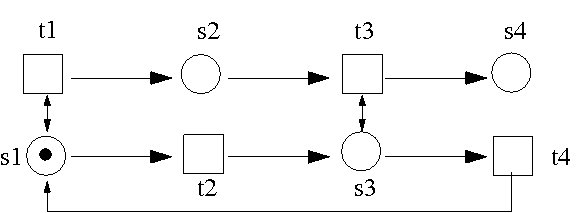
\includegraphics[width=0.5\textwidth]{omegaNet}
%%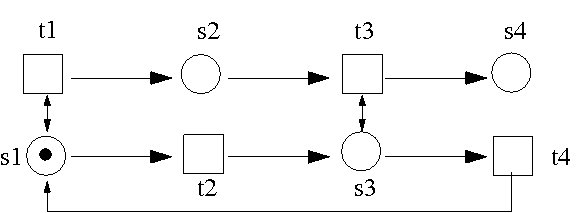
\epsfig{file=omegaNet,width=.5\textwidth}
\caption{A PT-net and configuration with an infinite number of reachable configurations} 
\label{fig:ptnet}
\end{figure}
%

Despite such examples, reachability in PT nets is decidable and can be
determined using an abstraction method called $\omega$-sequences, (see
e.g. \cite{DesR98}).  The main idea in determining $\omega$ sequences
is to define a partial order $\geq_{\omega}$ on configurations as
follows.  If configurations $C_1$ and $C_2$ are both reachable, $C_1$
and $C_2$ have tokens in the same set $PL$ of places, $C_1$ has at
least as many tokens in each place as $C_2$, and there exists a
non-empty $PL_{sub} \subseteq PL$, such that for each $pl \in
Pl_{sub}$ $C_1$ has strictly more tokens than $C_2$, then $C_1
>_{\omega} C_2$.  When evaluating reachability, if $C_2$ is reached
first, and then $C_1$ was subsequently reached, $C_1$ is abstracted by
marking each place in $PL_{sub}$ with the special token $\omega$ which
is taken to be greater than any integer.  If $C_1$ was reached first
and then $C_2$, $C_2$ is treated as having already been seen.

Tabling combined with partial order answer subsumption requires
slightly over 100 lines of code to model reachability in PT nets using
$\omega$-sequences.  Due to space restrictions, the program cannot be
fully described here, but the top-level reachability predicate is
shown in Figure~\ref{fig:ptnetcode}.  Despite its succinctness, it can
evaluate reachability in networks with millions of states in a few
minutes.  This use of tabling to determine reachability in PT nets can
be seen as a special case of tabling for abstract interpretation
(cf. \cite{KaKa93} and other works).  However the framework for answer
subsumption described here allows tabling to be used to efficiently
perform abstract interpretation within a general Prolog system
%
\begin{figure}
\begin{verbatim}
:- table reachable(_,po(omega_gte/2,omega_abs/3)).
reachable(InConf,NewConf):-
        reachable(InConf,NewConf),
        hasTransition(Conf,NewConf).
reachable(InConf,NewConf):- hasTransition(InConf,NewConf).
\end{verbatim}
\caption{Top-level predicate for PT net reachability}
\label{fig:ptnetcode}
\end{figure}

\subsubsection{Scalability for multi-valued and quantitative logics} \label{sec:mv}
\index{tabling!answer subsumption}
%
The technique of program justification (cf. e.g. \cite{PGDRR04}) has
been used for debugging tabled programs that cannot be debugged by
traditional means.  Here, we consider justification in the context of
the Silk system, currently under development at Vulcan, Inc.  Silk is
a commercial knowledge representation and rule system built on top of
Flora-2, which is implemented using XSB.  One of the salient features
of Silk is its default reasoning, which is based on a parameterized
argumentation theory evaluated under the well-founded
semantics~\cite{WGKFL09}.  One issue in using Silk is that knowledge
engineers must have a way of understanding the reasoning of the
system, a task complicated by the use of the well-founded semantics
and the intricacies of the argumentation theory.  We describe an
experimental approach to justification of Silk-style argumentation
theories using multi-valued logics.

As noted in~\cite{WGKFL09}, argumentation theories in Silk are usually
extensions of the default theories of Courteous Logic Programs (CLP)
and are based on two user-defined predicates: {\tt opposes/2} and {\tt
  overrides/2}.  Two atoms {\em oppose} each other if no model of a
program can contain both atoms: an atom and its explicit negation
oppose each other, but opposition can capture many other types of
contradictions.  Given two opposing atoms, one atom may {\em override}
the other, and so be given preference.  For atoms $A_1$ and $A_2$, if
$A_1$ and $A_2$ are both derivable and oppose each other but neither
overrides the other, $A_1$ and $A_2$ mutually {\em rebut} each other.
If in addition $A_1$, say, overrides $A_2$, $A_1$ {\em refutes}
$A_2$~\footnote{In~\cite{WGKFL09} argumentation theories are built on
  named rules, here we base them on derived atoms.}.  Within Silk and
Flora-2, the compilation of an argumentation theory ensures that
rebutted atoms have an undefined truth value, as do atoms that refute
themselves (i.e. if the {\tt overrides/2} predicate is cyclic).
However, for justification, it is meaningful to distinguish those
facts that are undefined due to a negative loop in the argumentation
theory from those that are undefined due to a negative loop in the
program itself.  In addition, it is meaningful to distinguish an atom
that is true because it overrides some other atom, from an atom whose
derivation does not depend on the argumentation theory.  Similar
distinctions can be made for default false literals leading to the
truth lattice shown in Figure~\ref{fig:courteous}.
\begin{figure}
\comment{
\small{
\begin{verbatim}
:- table defeated/1.
defeated(A):-  defeated_by(A,_B).       defeated(A):-  defeats(A,_B).

defeated_by(A,B):- refutes(B,A),B.      defeats(A,B):- refutes(A,B),B.	        
defeated_by(A,B):- rebuts(B,A),B.       defeats(A,B):- rebuts(A,B),B.		

refutes(A,B):- conflicts(A,B), overrides(A,B).
rebuts(A,B):- conflicts(A,B).

conflicts(A,B):- opposes(A,B),A.        conflicts(A,B):- opposes(B,A),A.
\end{verbatim}
}}
\centering
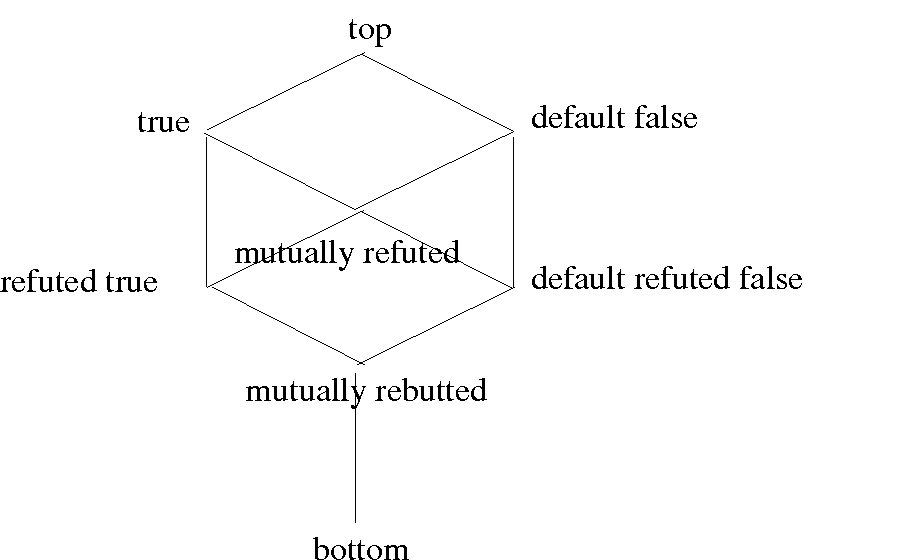
\includegraphics[width=0.45\textwidth]{courteous2}
%%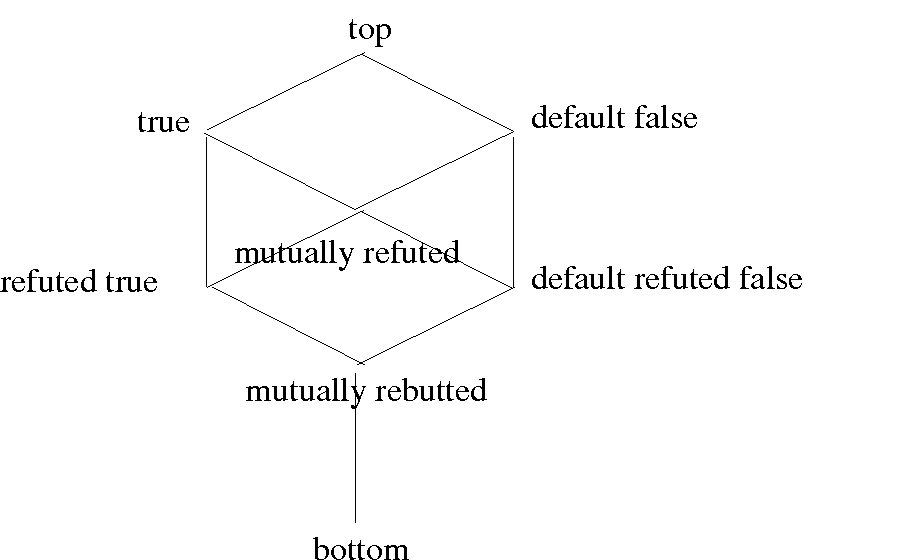
\epsfig{file=courteous2,width=.45\textwidth}
\caption{A Truth Lattice for a Simplified Version of Courteous Argumentation Theory} 
\label{fig:courteous}
\end{figure}
%

\subsection{Term-Sets}

XSB provides support for a programming technique for representing sets
of terms, called term-sets.  (While it is not closely related to
answer subsumption, it is partially implemented through tabling and a
table declaration, and so this facility is documented here.)

We begin in an example.  We can represent a set of Prolog terms by
using a particular term of the form \verb|{Var:Goal}| where Goal has
(only) \verb|Var| free in it.  Then we will use this \emph{set-term} to
represent the set of terms obtained by evaluating \verb|Goal| and
taking the values of \verb|Var| that are obtained.  I.e., they would
be the terms in the list \verb|L| returned by the Prolog call to
\verb|setof(Var,Goal,L)|. For example, the set-term:
\begin{verbatim}
{X : member(X,[a,b,c])}
\end{verbatim}
represents the set of terms \verb|{a,b,c}|.

Now a \emph{term-set} is a Prolog term that may contain set-terms as
subterms.  For example,
\begin{verbatim}
m({X:member(X,[a,b,c])},g(d,{Y:member(Y,[e,f,g])}),h)
\end{verbatim}
is a term-set, and it represents the set of terms obtained from it by
replacing (recursively) any embedded set-term by a term in that
set-term.  So the above term-set represents the 9 terms:
\begin{verbatim}
m(a,g(d,e),h)        m(a,g(d,f),h)        m(a,g(d,g),h)
m(b,g(d,e),h)        m(b,g(d,f),h)        m(b,g(d,g),h)
m(c,g(d,e),h)        m(c,g(d,f),h)        m(c,g(d,g),h)
\end{verbatim}
This example shows an advantage of this representation.  Say a
term-set has $k$ sub-set-terms each of which is of the member form in
this example where each member has a list of atoms of length $n$.  To
represent this set of terms explicitly takes $O(n^k)$ space, whereas
to represent them with the term-set takes only $O(n \times k)$ space.  So a
term-set representation can take exponentially less space than an
explicit representation.

It is relatively easy to write a predicate, {\tt member\_termset/2},
which takes a variable and a term-set
and non\-deterministically generates all concrete terms represented by
the term-set, called \emph{extensionalizing} the term-set.  Some care
must be taken since a call to goal to extensionalize a set-term may
itself return a term-set.  Also term-sets can be self-recursive and
thus represent infinitely many Prolog terms.  For example, consider
the term-set:
\begin{verbatim}
{X : p(X)} where
  p(a).
  p(f({X:p(X)})).
\end{verbatim}
This term-set represents the terms for which {\tt p/1} is true.  Now
{\tt p(a)} is true, so {\tt a} is in the term-set.  Since {\tt a} is
in \verb|{X:p(X)}|, then {\tt p(f(a))} is true because of the second
fact for {\tt p/1}, and so {\tt f(a)} is in the term-set.  And so on.
So this term-set contains the infinitely many terms:
\begin{verbatim}
a, f(a), f(f(a)), f(f(f(a))), ...
\end{verbatim}

A particularly interesting use of term-sets is in conjunction with
tabling.  Consider the term-set \verb|{X:p(1,2,X)}| where {\tt p/3} is
tabled.  If \verb|p(1,2,_}| has been called and so its table is
filled, then extensionalizing this term-set requires just a table
lookup; in some sense we can think of such a term-set as standing for
a pointer into a table to a set of terms.  This can be elegantly used
to solve an important problem in handling parse trees in context-free
parsing.

Consider the following DCG for the language {\tt a}*:
\begin{verbatim}
:- table a/3.
a(a(P1,P2)) --> a(P1),a(P2).
a(a) --> [a].
\end{verbatim}
which recognizes a string of {\tt a's} and constructs its parse trees.

To generate all answers, this DCG will take time exponential in the
length of the input string; not surprising since there are
exponentially many parses.  But say we give it an input string of $n$
{\tt a}'s followed by one {\tt b}.  In this case it will take
exponential time to fail, since it will construct all the
exponentially many partial parse trees for the initial $k$ {\tt a}'s.
We would like the parser in this case to fail in polynomial time.  We
can do this by representing the parse trees as a term-set during the
recognition of the string.  Then after the string is recognized, we
extensionalize the set-term that represents the parse trees.  In this
way we can get the behavior we want.  The set-term that represents the
parse trees for any grammar will be constructed in polynomial time;
the extensionalization of that term-set will take exponential time
only if there are exponentially many parses.

We can cause XSB to automatically use the term-set representation for
the grammar by adding to the above program the declaration:
\begin{verbatim}
:- table a(termset,_,_).
\end{verbatim}
which tells XSB to use the term-set representation of the first
argument of nonterminal {\tt a/3}.

With this declaration, the XSB compiler transforms the above program
into the following:
\begin{verbatim}
:- table a/3.

a(a(P1,P2),S0,S) :- '_$a'(P1,S0,S1),'_$a'(P2,S1,S).
a(a,S0,S1) --> 'C'(S0,a,S1).

:- table '_$a'/3 as subsumptive.
'_$a'({X:'_$a'(X,S0,S)},S0,S) :- a(_,S0,S).
\end{verbatim}
A new predicate {\tt '\_\$a'/3} has been introduced, and all calls to the
original predicate {\tt a/3} are replaced by calls to the new one.  It
is defined to call the original {\tt a/3} but to return the term-set
instead of the concrete parse tree in the argument declared to be a
term-set.

We can see that a call to {\tt a/3} in this new program will have
exactly as many answers as the corresponding call to {\tt a/2} in the
original recognizing DCG, since given values for {\tt S0} and {\tt S},
a call to {\tt '\_\$a'/2} returns only one value in its first
argument.  So a call to {\tt a/3} with have the polynomial complexity
of the recognizer.  So now when this representation is used, one gets
the concrete parse tree for a string by writing, for example:
\begin{verbatim}
| ?- a(Pts,[a,a,a,a,a,a,a],[]), member_termset(Parse,Pts).
\end{verbatim}
Here the term-set representing the parses for the sequence of {\tt
a}'s will be returned in the variable {\tt Pts}, and then {\tt
member\_termset} is used to extensionalize it
to the produce the actual explicit parse
tree.  With this way of handling parse trees in arbitrary context-free
grammars, the complexity of parsing to create the term-set is always
polynomial, and then extensionalizing the term-set may be exponential
if all parses are desired and there are exponentially many of them.
(In fact, if the grammar contains a rule such as \verb|A --> A|, there
may be infinitely many parses.)
Of course, if the parsing call to {\tt a/3} fails, then there is no
extensionalization to do, and the process is polynomial.

Note that the transformation uses subsumptive tabling for the newly
introduced auxiliary predicate.  This is important for this example,
since the parsing calls to {\tt '\_\$a'/3} will normally have {\tt S0}
bound and {\tt S} free, yet when extensionalizing the constructed
term-set to obtain the parse trees, the calls will have both {\tt S0}
and {\tt S} bound.  We do not want to recompute the parse during
extensionalizion, which would happen were we to use variant
tabling, and so we use subsumptive tabling.

Problems in graph traversal provide another example of the effective
use of term-sets.  For graph reachability, we have the very familiar:
\begin{verbatim}
:- table reach/2.
reach(X,Y) :- edge(X,Y).
reach(X,Y) :- reach(X,Z), edge(Z,Y).
\end{verbatim}
which is linear in the number of edges in the graph.  But say that we
now want to construct the path from X to Y when Y \emph{is} reachable
from X.  One simple way to do it (collecting the intermediate nodes in
the path in reverse order) is:
\begin{verbatim}
:- table path/3.
path(X,Y,[]) :- edge(X,Y).
path(X,Y,[Z|Path]) :- path(X,Z,Path), edge(Z,Y).
\end{verbatim}
For an acyclic edge graph, this works fine, but for a graph with
cycles, this will go into an infinite loop.  Indeed, it must, since in
a cyclic graph there \emph{are} infinitely many different paths between
some nodes.  However, we can use term-set to handle this situation
more flexibly.  We modify the above program by adding:
\begin{verbatim}
:- table path(_,_,termset).
\end{verbatim}
With this declaration, every call to {\tt path/3} (for a finite edge
graph) will terminate in time linear in the number of edges.  And all
the paths will be presented in the term-set returned in the third
argument.  Here we have an advantage similar to the one we had in the
grammar example above: if there is no path from our source to our
target node, we will find that out in linear time.  Without the
term-set declaration, this might take exponential time, while the
program builds all the paths to all the nodes that \emph{are} reachable
from our source node.  Also, if we want only \emph{one} possible path
from our source to our target, we can easily retrieve only one member
of the term-set during extensionalization, and the whole process is
still linear.

Now consider what happens with when the graph has cycles.  In this
case, the term-set may be recursive and represent the infinitely many
paths between nodes.  For example, the term-set representing all paths
from {\tt a} to {\tt a} in the graph with a single edge from {\tt a} to
{\tt a} will have the same structure as the example of an infinite
term-set given at the beginning of this subsection.  Once the path
term-set is constructed (in time linear in the number of edges for a
single source), producing paths reduces to processing the term-set
structure.  For example to generate all paths between nodes which do
not contain repeated intermediate nodes, one could write an
extensionalization predicate that passes a list of term-sets in the
process of being expanded, and refuse to re-expand one currently being
expanded.  This is the technique often used in Prolog without tabling
to compute reachability in cyclic graphs.

All of these examples can be seen as special cases of constructing
proof trees or justifications of goals.  Indeed, term-sets could be
effectively used in the construction of a justification or explanation
system.

\index{termination!subgoal abstraction}
\index{bounded rationality}
\index{termination!radial restraint}
\index{termination!answer count restraint}
\index{abstraction of terms!subgoal}
\index{abstraction of terms!answer}
\section{Tabling for Termination} \label{sec:tabling-termination}
%
As noted throughout this manual, tabling adds important termination
properties to programs and queries.  In this section we state more
precisely what these termination properties are, and how the
properties can be strengthened through declarations and settings for
{\em subgoal abstraction} and for sound bounded rationality through a
type of answer abstraction called {\em radial restraint} as well as by
limiting the number of answers to a subgoal through {\em \maxans{}
  restraint}.

Before proceeding, it is important to set the context for where issues
of termination may arise.  Consider first a pure normal program in
which every predicate is tabled.  This means a program where rules may
only call other rules, possibly through negation ({\tt tnot/1}, {\tt
  not\_exists/1} or {\tt u\_not/1} in XSB); but where there are no
calls to built-in all-solutions predicates, or other built-ins.  If
such a fully-tabled pure normal program does {\em not} have function
symbols, XSB will always terminate for any query.  For instance, XSB
will terminate for fully tabled pure datalog programs -- even if the
head of a rule is ``unsafe'' in that it contains variables that do not
occur in the body of that rule~\footnote{Evaluations that call
  non-ground negative literals will terminate through floundering,
  although this can be avoided in most cases by using {\tt
    not\_exists/1}.}.  Such programs are sometimes called datalog
programs.

While datalog programs are useful for certain kinds of knowledge
representation, they are not powerful enough for general programming
as they do not allow recursive structures such as lists.  Thus, for
the rest of this section we consider pure programs that may contain
function symbols.  Consider a pure definite program in which every
predicate is tabled.  Such a program would create a table for each
tabled subgoal (up to variance) exactly once if call variance were
used, and at most once if call subsumption were used.  In addition,
tabling guarantees that each answer will be returned to each call to a
tabled subgoal at most once.  This means that there are two sources of
non-termination.  Either there can be an infinite number of subgoals,
or there can be an infinite number of answers.\footnote{Here, forest
  of trees model of tabling (cf. Section~\ref{sec:forest-trace}) is
  being implicitly used.}

\paragraph{An Infinite Number of Subgoals}
%
If a definite program produces an infinite number of subgoals {\em
  but} has a finite number of answers, the program can be made to
terminate by abstracting the subgoal.  For instance, consider the
program fragment:
%
\begin{verbatim}
:- table p/1.
p(X) :- p(f(X)).
\end{verbatim}
%
The goal {\tt ?- p(1)} can create an infinite number of tabled
subgoals: {\tt p(f(1))}, {\tt p(f(f(1)))}, {\tt p(f(f(f(1))))} and so
on.  Note that since all of the subgoals are ground, none subsume one
another, so that call subsumption will not help here. (Although call
subsumption is extremely useful in other circumstances, and would help
if the goal were {\tt ?- p(X)}).

\paragraph*{Infinite Answers}
%
Of course, subgoal abstraction can't handle cases where there are an
infinite number of answers, as in the program fragment:
%
\begin{verbatim}
p(f(X)) :- p(X).
\end{verbatim}
%
when given the query {\tt ?- p(X)}.  

We consider each case in turn.

\subsection{Term Size Abstraction in XSB} \label{sec:size-metric}
\index{abstraction of terms!size metric}
%
Both subgoal and answer abstraction in XSB are based on limiting the
size of any argument of a term $T$ that forms a subgoal or answer.
The specific definition of size used is slightly complicated, but
offeres advantages discussed below.  Each argument $T_a$ of $T$ is
traversed as follows.  The size of $T_i$ is initialized to 0, then
$T_a$ is traversed from left to right.  Each time a non-constant
functor or list symbol is encountered, the size of $T_i$ is
incremented by 1 -- regardless of the type of functor symbol that is
encountered.  If the size of $T_a$ exceeds the associated size limit
for $T$ (as declared in the next section), all further non-constant
functor symbols encountered in $T_i$ will be abstracted (rewritten as
free variables).  Once $T_a$ has been fully traversed, further
arguments of $T$ will be traversed in the exact same manner.

%, with one
%important exception.  The functor symbols will be abstracted {\em
%  only} if they also occur at depth greater than 0.

\begin{example} \label{ex:term-size-abs}
Applying the above definition of size abstraction with limit 2 to the
term 

{\tt p(d(e(1),a,f(c$_1$)),b,g(c$_2$),[c$_3$,[c$_4$,c$_5$]))}

\noindent
  produces the term 

{\tt p(d(e(X$_1$),a,X$_2$),b,g($c_2$),[$c_4$|X$_3$])}.  

\noindent
In the traversal, the size limit is reached once the {\tt e/1} functor
is encountered.  To the right of {\tt e/1}, all non-constant functor
symbols are abstracted when they occur at depth greater than 0.  This
causes {\tt f/1} to be abstracted, as it occurs at depth 1; however
{\tt g/1} in the third occurs at depth 0, and so is retained.
Similarly in the fourth argument, the outer list symbol and head is
preserved, while the tail of the list is abstracted.
\end{example}

Example \ref{ex:term-size-abs} indicates that the size abstraction
used in XSB excludes symbols of depth 0, and so is something of a
hybrid approach, although we continue to call it size abstraction.

Other metrics could be used, such as term depth, which would offer
conceptual clarity.  However size-based abstraction allows
finer-grained optimization than depth-based abstraction and offers the
following general advantages.
\begin{itemize}
\item From the point of view of implementation, the abstraction can be
  perfomed with manner that has minimal if any impact on the speed of
  XSB's tabling engine. 
\item By not abstracting functor symbols at depth 0 and by abstracting
  each argument individually, both multi-argument indexing and star
  indexing of subgoals will be often be preserved.
\end{itemize}

\subsection{Subgoal Abstraction} \label{sec:subg-abs}
\index{abstraction of terms!subgoal}
%
In a nutshell, subgoal abstraction allows a goal like {\tt
  p(f(f(f(1))))} to be rewritten as 

{\tt p(f(f(X))),X = f(1)}.  

\noindent
If all subgoals that have a term size -- or term depth -- over a given
finite threshold are abstracted, any query can produce only a finite
number of subgoals (since there are a finite number of predicate,
function and constant symbols in any program). If a program has a
finite well-founded model, it can be shown that any query to a program
will terminate if that program uses subgoal abstraction~\cite{RigS14}.
%
For normal programs, the situation is not much different at a
conceptual level.  A goal such as {\tt tnot(p(f(f(f(1)))))} would
execute as {\tt p(f(f(X)))} and then ensure that none of the answers
to this goal have a binding for {\tt X} that allows it to unify with
{\tt f(1)}.  Using this intuition, it can be shown that if a program
has a well-founded model with a finite number of true or undefined
answers it will terminate using tabling with subgoal
abstraction~\cite{RigS13,RigS14}.

Despite its theoretical power, subgoal abstraction can also cause
problems if used indiscriminately.  For instance, if the second
argument of the subgoal
%
\begin{verbatim}
?- member(e,[a,b,c,d,e])
\end{verbatim}
%
is abstracted forming the goal
%
\begin{verbatim}
?- member(e,[a,b,c|X])
\end{verbatim}
%
leading to an infinite number of answers.  a goal that terminates
without abstraction will not terminate after abstraction.  Note that
any program containing {\tt member/2} and at least one constant does
not have a finite model (although any given ground query will have a
finite number of answers).  While an experienced programmer would not
usually table {\tt member/2}, he well may want to table a grammar or
other program that performs recursion through a finite structure.

\index{tripwires!max\_table\_answer\_size}
\subsubsection{Declaring Subgoal Abstraction}
%
% The implementation of subgoal abstraction in XSB is still in progress.
% and may be changed in future versions as we gain experience in how
% subgoal abstraction is best used in practice.  

XSB can perform subgoal abstraction based on the size limit described
above.  It will do so for goals called positively, but not for goals
called negatively as this would give rise to unsound negation.  Thus a
goal $G$ inside a construct such as {\tt tnot/1} or {\tt
  not\_exists/1} will throw an exception (or suspend into break mode)
if it surpasses the specified term size. In addition, subgoal
abstraction is only implemented for call variance, {\em and applies
  equally to all functors, whether they are lists or non-lists}.
Despite these restrictions, a tabled evaluation can be still
guaranteed to terminate for queries to safe programs
(cf.~\cite{RigS13}).

\index{Prolog flags!{\tt max\_table\_subgoal\_action}} 
\index{Prolog  flags!{\tt max\_table\_subgoal\_size}} 

Subgoal abstraction can be declared by setting a value for the maximum
size of a subgoal and for the action to take when a subgoal is
encountered that reaches that size.
%
\bi
\item {\bf size} The maximum size can be set to $n$ for a set of
  predicates $\langle PredSpec \rangle$ by including the specifier
  {\tt subgoal\_abstract(n)} as part of the tabling declaration

{\tt :- table $\langle PredSpec\rangle$  as ...,subgoal\_abstract(n),...}

  Specifying {\tt subgoal\_abstract(0)} turns abstraction off for
  predicates in $\langle PredSpec \rangle$.  The size can also be set
  globally by seting the flag {\tt max\_table\_subgoal\_size} to the
  desired maximal size.  If the subgoal size has been set of a given
  predicate via a tabling declaration the declared size will override
  the global size.

\item {\bf action} When a subgoal is encountered of maximum size,
  abstraction is enabled if the Prolog flag {\tt
    max\_table\_subgoal\_action} to {\tt abstract}.  Other possible
  values for the action are {\tt error} and {\tt suspend}
  (cf. pg. \pageref{prolog-flags} ff.).  \ei

\noindent
Unless otherwise specified, XSB starts up with {\tt
  max\_table\_subgoal\_action} set to {\tt error} and {\tt
  max\_table\_subgoal\_size} set to 0, indicating it is turned off.
Under this default behavior, XSB will throw an error if a subgoal has
size greater than {\tt max\_table\_subgoal\_size}.  As an alternative
to setting flags, subgoal abstraction can be set by calling XSB with
the command-line arguments {\tt --max\_subgoal\_action a} and {\tt
  --max\_subgoal\_size n} with {\tt a} the desired action and {\tt n}
the desired size limit.

\subsection{XSB's Approach to Bounded Rationality} \label{sec:restraint}
\index{abstraction of terms!answer}
\index{bounded rationality}
%
Bounded rationality is a subfield of Artificial Intelligence that
studies how the reasoning performed by a computation can be
automatically bounded so that an agent or other program can be
guaranteed to arrive at a decision ``quickly''.  By bounding
reasoning, an agent may be used in a setting that requires reactivity
or where a simulation of human reasoning is needed.

Thus, the approximation that XSB computes is {\em
  informationally sound} in the sense that no incorrect answer will be
derived, although the truth value of some atoms won't be known that
might have been if the size bound had been set higher.  

XSB's approach to bounded rationality computes a finite approximation
to the well-founded model that is {\em informationally sound} in the
sense that no incorrect answer will be derived, although the truth
value of some atoms won't be known. In other words, if bounded
rationality is employed, it can be guaranteed that only a finite
number of answers will be derived~\cite{GroS13}.  Furthermore, any
true atom that XSB derives is true in the well founded model of a
program; and any goal that fails is false in the well-founded model.
However, by bounding rationality XSB's search is restrained so that it
will not fully explore certain subderivations and so may consider as
undefined some atoms that are true or false in the well-founded model.
We sometimes call this approach to bounded rationality {\em
  restraint}.  Currently XSB supports both {\em radial restraint} and
{\em \maxans{} restraint}

\index{restraint!radial}
\subsubsection{Radial Restraint Through Answer Abstraction}
Radial restraint resembles subgoal abstraction (Section
\ref{sec:subg-abs}) in certain ways, as can be seen in the following
example. If the query {\tt p(X)} to the program
%
\begin{verbatim}
p(f(X)) :- p(X).  
p(0).
\end{verbatim}
%
were evaluated using radial restraint with a size limit of 3, the
answers, {\tt p(0)}, {\tt p(f(0))}, {\tt p(f(f(0)))} and {\tt
  p(f(f(f(X))))} would be generated; {\bf {\em however}}, {\tt
  p(f(f(f(X))))} would have the truth value of {\em undefined}.  Note
that by abstracting in this way, both of the goals {\tt
  p(f(f(f(0))))}, and {\tt p(f(f(f(1))))} will unify with {\tt
  p(f(f(f(X))))} and so will succeed with a truth value of {\em
  undefined}.  Similarly {\tt tnot(p(f(f(f(0)))))}, and {\tt
  tnot(p(f(f(f(1)))))} will both succeed with a value of {\em
  undefined} (perhaps better called {\em unknown} in this context).
%
It can be seen that since all predicates and function symbols have a
maximum arity (256 in XSB) bounding the size of an answer ensures that
only a finite number of answers are returned
\footnote{If a program has a infinite number of true answers and a
  finite number of false answers, one possible approach might be to
  ``dualize'' the program so that only false answers are computed.
  Note that since most programs with function symbols have an infinite
  number of both true and false answers, this approach won't work in
  general.}.

Semantically when radial restraint is used, XSB computes an
approximation to the three-valued well-founded model of a program,
called a {\em restrained model}.  To see this, suppose the proof of a
query $Q$ does not depend on negation.  If $Q$ has a derivation that
does not require any answers whose size is greater than $n$, it is
proven as usual.  Similarly, if $Q$ is false in the well-founded model
of a program, and none of the subgoals explored in the derivation of
$Q$ derive answers whose size is greater than $n$, XSB will derive
that $Q$ is false.  The higher the size bound that is set, the better
the approximation.  Due to undecidability, there is no way to know in
general what size to set for answer abstraction, or whether any bound
needs to be set at all.

If a restrained model is derived, answers that are directly undefined
through radial restraint can be desinguished from answers that are
undefined in the well-founded model of a program, or for other reasons
such as unsafe negation.  If an answer $A$ was abstracted due to a
size check, the query {\tt get\_residual(A,Delay)} would bind {\tt
  Delay} to a list containing the atom {\tt radial\_restraint}, where
{\tt radial\_restraint/0} is simply a predicate defined as

{\tt radial\_restraint:- tnot(radial\_restraint)}

%\noindent
%which in a delay list indicates that an answer was made undefined
%through bounded-rationality based answer abstraction.

\index{tripwires!max\_table\_answer\_size}
\paragraph*{Using Radial Restraint}
%
Radial restraint is currently implemented only for tabling with call
variance.  However it works with most other tabling features, such as
call abstraction, and incremental tabling.
%
Similarly to the use of subgal abstraction, answer abstraction is the
implementational basis of radial restraint.  {\em It is important to note
that the size limit applies to the answer substitution, not to the 
of the answer itself.}

\begin{example}
Suppose an answer size limit is set to 1, and consider the goal {\tt
  p(X)}.  The answer {\tt p(s(s(0)))} has size 2 and so would be
abstracted to {\tt p(s(X$_1$))} as expected, as the corresponding
abswer substitution is $X = s(s(0))$.  However for the goal {\tt
  p(s(X))} the answer substitution for the answer {\tt p(s(s(0)))} is
$X = s(0)$ which has a size of only 1 and so this answer would not be
abstracted in the context of this subgoal.  Despite this difference in
how the size metric is computed, the termination and approximation
properties of radial restraint still hold.
\end{example}

Radial restraint can be declared by setting a value for the maximum
size of an answer and for the action to take when an answer is
encountered that reaches that size.
%
\bi
\item {\bf size} The maximum size can be set to {\tt n} for a set of
  predicates via including the specifier {\tt answer\_abstract(n)} as
  part of their tabling declaration

{\tt :- table $<PredSpec>$ as ...,answer\_abstract(n),...}

  Specifying {\tt answer\_abstract(0)} turns answer abstraction off
  for predicates in $\langle PredSpec \rangle$.  The size can also be
  set globally by seting the flag {\tt max\_table\_answer\_size} to
  the desired maximal size.  If the answer size of a given predicate
  has been set via a tabling declaration, the predicate-specific
  declared size will override the global size.

\item {\bf action} When an answer is encountered of maximum size,
  abstraction is enabled if the Prolog flag {\tt
    max\_table\_answer\_action} to {\tt bounded\_rationality}.  Other
  possible values for the action are {\tt error}, {\tt suspend}  and {\tt fail}
  (cf. Section \ref{sec:tripwire} for further information).  \ei


\index{Prolog flags!{\tt max\_table\_answer\_action}} 
\index{Prolog flags!{\tt max\_table\_answer\_size}}
%
Unless otherwise specified, XSB starts up with {\tt
  max\_table\_answer\_size\_action} set to {\tt error} and {\tt
  max\_table\_answer\_size} set to 0.  
%

\subsubsection{\MAXANS Restraint} \label{sec:answer-count-restraint}
\index{tripwires!max\_answers\_for\_subgoal}
\index{restraint!answer count}

As discussed above, finite termination can always be ensured through a
mixture of subgoal abstraction and radial restraint.  Alternately, it
can also be ensured through subgoal abstraction and \maxans()
restraint.  

\begin{example} \label{ex:maxans}
Consider the program

\begin{verbatim}
:- table p/4.
p(M,N,X,Y):- between(1,M,X),between(1,N,Y).
\end{verbatim}

\noindent
and query {\tt p(3,3,Y,Z)}: it is easy to see that 9 answers will be
produced.  However, if \maxans{} restraint is used to restrict the
maximal number of answers to each subgoal to 5, the first 5 answers
computed above will be returned, along with a new answer:

{\tt p(3,3,Y,Z)}

\noindent
whose truth value is undefined, with the atom 
%
{\tt \maxUans\_restraint} in its delay list.
\end{example}

Using the arguments from the previous section, it is easy to see that
\maxans{} restraint ensures sound finite termination when used with
subgoal abstraction.  However Example~\ref{ex:maxans} also illustrates
on a small scale how \maxans{} restraint can be used to soundly
complete a subgoal $S$ once a minimal number of answers have been
derived, even if $S$ has a large, but finite number of answers.

\paragraph*{Using \MAXANS{} Restraint}
\Maxans{} restraint is currently implemented only for tabling with call
variance.  However it works with most other tabling features, such as
call abstraction, and incremental tabling.

Currently, \maxans{} restraint can only be set by global flags as
follows.
\bi
\item {\bf size} The size can be set globally via the flag {\tt
  max\_table\_answer\_size} to the desired maximal size.  Setting the
  flag to 0 turns off \maxans{} restraint.

\item {\bf action} When an answer is encountered of maximum size,
  abstraction is enabled if the Prolog flag {\tt
    max\_table\_answer\_action} to {\tt bounded\_rationality}.  Other
  possible values for the action are {\tt error} and {\tt suspend}
  (cf. Section \ref{sec:tripwire} for further information).  
\ei

\subsubsection{Justifying or Explaining Restraint}

An atom affected directly by radial or answer count restraint has in
its delay list either the atom {\tt radial\_restraint} or {\tt
  answer\_count\_restraint}.  The indirect dependency of an atom on a
form of restraint can be obtained either thorugh the predicate {\tt
  explain\_u\_val/3}, or {\tt get\_residual\_sccs/[3,5]}.  Both of
these predicates traverse the residual dependency graph to provide
information about why a literal is undefined.

\index{residual dependency graph}
\predref{explain\_u\_val/3}
\predref{get\_residual\_sccs/3}
\predref{get\_residual\_sccs/5}

%--------------------------------------------------------------------
\section{Incremental Table Maintenance} \label{sec:incremental_tabling}
%====================================================

\index{tabling!incremental}

XSB allows the user to declare that the system should maintain the
correctness of a given table with respect to dynamically changing
facts and rules through so-called {\em incremental
  tables}~\cite{SaRa05,Saha06,Swif14}.
%A table $T$ is {\em incremental} if XSB ensures that its answers are
%  consistent with all dynamic facts and rules upon which $T$ depends
%  (subject to transactionality conditions explained below).
After a database update or series of updates $\Delta$, an incremental
table $T$ that depends on $\Delta$ is by default updated
transparently: that is $T$ and all tables upon which $T$ depends are
automatically updated (if needed) whenever a future subgoal calls $T$.
Alternately, if circumstances require it, a table can be updated
immediately upon a database change or by issuing an explicit command
to update all tables that depend on $\Delta$.
%
In either case, incremental tabling brings XSB closer to the
functionality of deductive databases.  If tables are thought of as
materialized database views (or snapshots), then the incremental table
maintenance subsystem enables incremental view maintenance; also as
discussed below, if choice points are thought of as database cursors
then incremental tabling also provides view consistency~\footnote{In
  the current version of XSB, there are certain restrictions on how
  incremental tabling can be used:
  cf. Section~\ref{sec:tabling-compatibility}.}.

\subsection{Transparent Incremental Tabling} \label{sec:incr_examples}

To demonstrate incremental table maintenance (informally called {\em
  incremental tabling}), consider first the following simple program
that does not use incremental tabling:
\begin{verbatim}
:- table p/2.
p(X,Y) :- q(X,Y),Y =< 5.

:- dynamic q/2.
q(a,1).    q(b,3).   q(c,5).    q(d,7).
\end{verbatim}
and the following queries and results:
\begin{verbatim}
| ?- p(X,Y),writeln([X,Y]),fail.
[c,5]
[b,3]
[a,1]

no
| ?- assert(q(d,4)).

yes
| ?- p(X,Y),writeln([X,Y]),fail.
[c,5]
[b,3]
[a,1]

no
\end{verbatim}
%
In this program, the table for {\tt p/2} depends on the contents of
the dynamic predicate {\tt q/2}.  We first evaluate a query, {\tt
  p(X,Y)}, which creates a table.  Then we use {\tt assert/1} to add a
fact to the {\tt q/2} predicate and re-evaluate the query.  We see
that the answers haven't changed, because the table is already created
and the second query just retrieves answers directly from that
existing table.  However the answers are inconsistent with the model
of {\tt p/2} after the assert.  I.e., if the table didn't exist
(e.g. if {\tt p/2} weren't tabled), the answer {\tt [d,4]} would also
be derived.  Without incremental table maintenance, the only solution
to this problem is for the XSB programmer to explicitly abolish a
table whenever changing (with assert or retract) a predicate on which
the table depends.
%
By declaring that the tables for {\tt p/2} should be incrementally
maintained, XSB automatically keeps the tables for {\tt p/2} correct.

%
Consider a slight rewrite of the above program:
\begin{verbatim}
:- table p/2 as incremental.
p(X,Y) :- q(X,Y),Y =< 5.

:- dynamic q/2 as incremental.
q(a,1).    q(b,3).    q(c,5).     q(d,7).
\end{verbatim}
in which {\tt p/2} is declared to be incrementally tabled
% (with {\tt  :- table p/2 as incremental}) 
and {\tt q/2} is declared to be both dynamic and incremental, meaning
that an incremental table depends on it.
%~\footnote{The declarations {\tt use\_incremental\_tabling/1} and
%  {\tt use\_incremental\_dynamic/1} are deprecated from Version 3.3 of
%  XSB forward -- in other words backwards compatibility will be
%  maintained for a time, but these declarations will not be further
%  supported.}.  
Consider the following goals and execution:
\begin{verbatim}
| ?- import incr_assert/1 from increval.
yes
| ?- p(X,Y),writeln([X,Y]),fail.
[c,5]
[b,3]
[a,1]

no
| ?- incr_assert(q(d,4)).

yes
| ?- p(X,Y),writeln([X,Y]),fail.
[d,4]
[c,5]
[b,3]
[a,1]

no
\end{verbatim}
\noindent
The transparent approach to incremental updating works as follows.
When {\tt incr\_assert/1} is called, it sparks an invalidation
phase in which tables that depend on {\tt q(d,4)} are marked as {\em
  invalid} (i.e., possibly inconsistent with respect to underlying
dynamic code).  An {\em Incremental Dependency Graph (IDG)} is used to
obtain the right tables to invalidate.  However, if the invalidation
phase finds an affected table that is incomplete, a permission error
is thrown, since it is unclear whether sensible semantics can be given
to updating a subgoal that is incomplete.  After the invalidation
phase is completed, when/if a subgoal calls an invalid table $T$ the
engine interrupts itself to recompute $T$ and any tables upon which
$T$ depends.  On the other hand, if no calls are ever made to an
invalid incremental table $T'$, $T'$ will never incur the cost of an
update.

\subsubsection{View Consistency} \label{sec:view-consistency}
%
As described above, transparent incremental tablings's use of lazy
updating ensures that a new query $Q$ will always be consistent with
the state of the dynamic code at the time $Q$ is called.  However,
transparent incremental tabling enforces a stronger property of view
consistency similar to those of database systems: that answers to a
query $Q$ should be those derivable at the time $Q$ was called, {\em
  and should not be affected by any updates}.
%Accordingly, the ISO standard for Prolog~\cite{ISO-Prolog} specifies
%that an update $\upsilon$ to dynamic code should not affect the
%behavior of choice points that were created before $\upsilon$.
Because XSB's incremental tabling does not allow updates that affect
tables that are still being computed, supporting view consistency
effectively means ensuring consistency for choice points into
completed incremental tables.  As such choice points correspond to
database cursors, we term them {\em Open Cursor Choice Points,
  (OCCPs)}.

XSB's support for view consistency is designed so that no perceptable
overhead in incurred if there are no OCCPs whose view needs to be
maintained.  Not surprisingly, numerous long-lived OCCPs whose views
need to be maintained across updates causes an overhead for the
engine, a situation that is in some sense similar to the cost of
maintaining views for cursors in database system.

%----------------------------------------------------------------
\comment{
In addition to the success continuations that are standard in most
languages, Prolog has failure continuations -- choice points to take
upon backtracking.  The presence of these failure continuations leads
to an issue of view consistency, even within a single-threaded
computation.  Suppose that a user
%
\begin{enumerate}
\item Makes a query to a completed incrementally tabled subgoal $Q$.
  $Q$ has more than one solution and the first one is returned,
  leaving a choice point into the table for $Q$.
\item Makes an update to dynamic code upon which $Q$ depends
\item Makes another query to $Q$
\end{enumerate}
%
What is the relation between the queries and the update.  Presumably,
the first query in step 1) should not reflect the changes made in step
2) if a user backtracks for further answers to that query -- this can
be seen as ensuring view consistency.. However it is less clear
whether the second query to $Q$ in step 4) should return the same
answers as the first query in step 1), or whether the second query
should reflect the database update.  Arguments can be made for either
approach.
%
\begin{itemize}
\item {\em Prolog-style semantics} If the second query reflects the
  database change, it is consistent with the database, but is not
  consistent with the first query~\footnote{This approach could be
    viewed as an extension of the ISO semantics for dynamic code in
    Prolog, which XSB does not currently support.};
\item {\em Delayed update semantics} If the second query does not
  reflect the dynamic code change, it is consistent with the first
  query but not with the dynamic code change.
\end{itemize}
%
XSB chooses the latter of these approaches.  If a user has failure
continuations into a query $Q$, then $Q$ and all tables that depend on
$Q$ will not be updated until these failure continuations have been
exhausted or removed.  However, all updates are ensured to be applied
once this is the failure continuations are removed.
}

%----------------------------------------------------------------

\subsection{Updating in a Three-Valued Logic}
%
As discussed earlier in this chapter, answers that are undefined in
the well-founded semantics are represented as conditional answers.
Beginning with version 3.3.7, incremental updates work correctly with
conditional answers~\footnote{Before Version 3.3.7, incremental
  updates only worked correctly on stratified tables: those with only
  unconditional answers.}.  Nno special care needs to be taken for
updating in the well-founded semantics as the following example
illustrates.
%conditional answers, and they can be updated through any of the
%previously described methods.  The following example illustrates one
%such approach.

\begin{verbatim}
:- dynamic data/1 as incremental.

:- table opaque_undef/0 as opaque.
opaque_undef:- tnot(opaque_undef).

:- table p/1 as incremental.
p(_X):- opaque_undef.
p(X):- data(X).
\end{verbatim}
%
Note that {\tt opaque\_undef/1} upon which {\tt p/1} depends is
explicitly declared as opaque~\footnote{An {\em opaque} predicate $P$
  is tabled and is used in the definition of some incrementally tabled
  predicate but should not be maintained incrementally.  In this case
  the system assumes that the programmer will abolish tables for $P$
  in such a way so that re-calling it will always give semantically
  correct answers.}.  When the above program is loaded, XSB will
behave as follows.
%
{\small
\begin{verbatim}
| ?- p1(1).

undefined
| ?- incr_assert(data(1)).

yes
| ?- p1(1).

yes
| ?- incr_retract(data(1)).

yes
| ?- p1(1).

undefined
| ?- get_residual(p1(1),C).

C = [opaque_undef]
\end{verbatim}
}
%

\subsection{Eager Incremental Tabling}~\label{sec:incr-eager}
%
Despite the advantages of transparent incremental tabling, there are
special circumstances when it may be better to update tables eagerly
rather than when (and if) they are called.  For instance, if updates
and queries are expected to occur at different times, performing eager
updates may improve query time.  In addition, if incremental tables
are accessed via table inspection predicates
(cf. Chapter~\ref{sec:TablingPredicates}) rather than by queries,
inconsistent answers may be obtained.  

\paragraph{An Eager Updating Approach}
%
Usually, best way to eagerly update tables is to use the {\tt
  incr\_assert/1} and {\tt incr\_retract(all)/1}
predicates as discussed above.  When the updates are finished, the
command {\tt incr\_table\_update/0} is then called, which updates all
tables that depend on any changed dynamic rules or facts.  The
following execution for our running program shows an example of this.

\begin{verbatim}
| ?- import incr_assert/1, incr_table_update/0 from increval.

yes
| ?- p(X,Y),writeln([X,Y]),fail.
[c,5]
[b,3]
[a,1]

no
| ?- incr_assert(q(d,4)), incr_assert(q(d,1)), 

yes
| ?- incr_table_update.

| ?- p(X,Y),writeln([X,Y]),fail.
[d,4]
[d,1]
[c,5]
[b,3]
[a,1]

no
\end{verbatim}
\noindent
As discussed, calling {\tt incr\_table\_update} causes the cost of
updating incremental tables to be immediately incurred, and ensures
that table inspection primitives show correct results.  However,
tables are updated and their views preserved even if the tables may
not be accessed before further updates are made.

\subsubsection{An Immediate Approach}
%
A final approach is to use the predicates {\tt incr\_assert\_update/1}
and {\tt incr\_retract(all)\_update/1}, which force immedidate updates
of invalidated tables.  While simple, this approach should only be
used in special circumstances, as calling {\tt incr\_assert\_update/1}
twice could cause tables to be updated twice rather than once.

\comment{
 We note, however, that the use of these predicates is much
less common than direct queries to tables; but if using table
inspection predicates on incrementally maintained tables, the user
should ensure that the tables have been eagerly updated as described
below in Section~\ref{}.  should ensure that {\tt
  incr\_table\_update/0} is called before inspecting the tables.

Here again we call {\tt p(X,Y)} and generate a table for it and its
answers.  Then we update {\tt q/2} by using the incremental version of
assert, {\tt incr\_assert/1}, which was explicitly imported.  Now when
we call {\tt p(X,Y)} again, the table has been updated and we get the
correct answer.

In this case after every {\tt incr\_assert/1} and/or {\tt
  incr\_retract(all)/1}, the tables are incrementally updated to
reflect the change.  The system keeps track of what tabled goals
depend on what other tabled goals and (incremental) dynamic goals, and
tries to minimize the amount of recomputation necessary.
Incrementally tabled predicates may depend on other tabled predicates.
In this case, those tabled predicates must also be declared as
incremental (or opaque).The algorithm used is described
in~
}
\subsubsection{Declaring Predicates to be Incremental}
%
In XSB, tables can have numerous properties: such as {\em subsumptive,
  variant, incremental, opaque, dynamic, private}, and {\em shared},
and can use answer subsumption or call abstraction.  XSB also has
variations in forms of dynamic predicates: {\em tabled, incremental,
  private}, and {\em shared}.  XSB extends the {\tt table} and {\tt
  dynamic} compiler and executable directives with modifiers that
allow users to indicate the kind of tabled or dynamic predicate they
want.  For example,
%
\begin{verbatim}
:- table p/3,s/1 as subsumptive,private.

:- table q/3 as incremental,variant.

:- dynamic r/2,t/1 as incremental.
\end{verbatim}
%We note that
%\begin{verbatim}
%:- table p/3 as dyn.
%and
%:- dynamic p/3 as tabled.
%\end{verbatim}
%are equivalent.

In the current version of XSB, incremental tabling works with subgoal
abstraction, answer abstraction, and well-founded negation.  However
several combinations involving incremental tabling are not supported
and will throw an error (cf. page \pageref{table-declaration} and page
\pageref{dynamic-declaration}, respectively). Incremental tabling has
not yet been ported to the multi-threaded engine and and it currently
works only for predicates that use both call and answer variance.

\index{tries!and incremental tabling}
\subsection{Incremental Tabling using Interned Tries} \label{sec:incr-update-tries}
%
Sometimes it is more convenient or efficient to maintain facts in
interned tries rather than as dynamically asserted facts
(cf. Chapter~\ref{chap:tries}).  Tables based on interned tries can be
automatically updated when terms are interned or uninterned just as
they can be automatically updated when a fact is asserted or
retracted.  Consider the example from Section~\ref{sec:incr_examples}
rewritten to use interned tries.  As usual, an incrementally updated
table is declared as such:
%
\begin{verbatim}
:- table p/2 as incremental.
p(X,Y) :- trie_interned(q(X,Y),inctrie),Y =< 5.
\end{verbatim}
%
However, the declaration for dynamic data changes: rather than using
the declaration 
\begin{center}
{\tt :- dynamic q/2 as incremental}
\end{center}
a trie is specified as incremental in its creation.
%
\begin{center}
{\tt  trie\_create(Trie\_handle,[incremental,alias(inctrie)])}
\end{center}
%
As described in Chapter~\ref{chap:tries}, the trie handle returned is
an integer, but can be aliased just as with any other trie.  The trie
may then be initially loaded:
%
\begin{verbatim}
	trie_intern(q(a,1),inctrie),trie_intern(q(b,3),inctrie),
	trie_intern(q(c,5),inctrie),trie_intern(q(d,7),inctrie).
\end{verbatim}
%
At this stage a query to {\tt p/2} acts as before:
%
\begin{verbatim}
| ?- p(X,Y),writeln([X,Y]),fail.
[c,5]
[b,3]
[a,1]
\end{verbatim}
%
The following sequence ensures that {\tt p/2} is incrementally updated
as {\tt inctrie} changes:
%
\begin{verbatim}
| ?- import incr_trie_intern/2.

yes
| ?- incr_trie_intern(inctrie,q(d,4)).

yes
| ?- p(X,Y),writeln([X,Y]),fail.
[d,4]
[c,5]
[b,3]
[a,1]

no
\end{verbatim}
%
Given the proper directives to make a trie incremental, transparent
incremental tabling works for changes made to interned tries just as
it does for regular dynamic code and for trie-indexed dynamic code.
There are also the predicates {\tt incr\_trie\_intern\_update/2} and
{\tt incr\_trie\_unintern\_updatesl/2} which immediately update
dependent tables.

\index{Incremental Dependency Graph (IDG)}
\subsection{Abstracting the IDG for Better Performance} \label{sec:IDG-abs}
As mentioned above, incremental table mantenance makes use of an IDG.
Specifically, the nodes of the IDG are the incrementally tabled
subgoals; and each such table contains information about its incident
edges: those subgoals upon which a node directly depends or directly
affects.  While the IDG is a critical data structure to efficiently
update incremental tables, in certain situations constructing the IDG
can cause non-trivial overheads in query time and table space.  These
overheads can be addressed in many cases by {\em abstracting} the IDG.
When a tabled subgoal $S$ is called, rather than creating an edge
between $S$ and its nearest tabled ancestor $S'$ (if any), one could
abstract $S$, $S'$ or both, potentially collapsing a large number of
nodes and edges of the IDG.  If $S$ is an incremental table, then
performing subgoal abstraction on $S$ as introduced in
Section~\ref{sec:tabling-termination}, will abstract the IDG -- rather
than having $n$ nodes $S_1,\ldots,S_n$ and their associated links, the
IDG will contain a single node $abstract(S)$.  However, subgoal
abstraction will not work to abstract the leaf nodes of the IDG, which
are subgoals to non-tabled dynamic incremental predicates.

In \version{} of XSB, IDG nodes for dynamic incremental predicates may
undergo depth abstraction: given a subgoal $S$ and integer $k$,
subterms of $S$ with depth $k+1$ are replaced by unique new variables.
For instance, abstracting
%the term 
{\em q(f(1))} at level 1 gives {\em q(f(X$_1$))}; abstracting at level
0 gives {\em q(X$_1$)}.
%
Figure~\ref{fig:abstraction} illustrates an important case where
abstracting dynamic incremental predicates can be critical to good
performance for incremental tabling.  In the case of left-linear
recursion, if no abstraction is used a new node will be created for
each call to {\tt edge/2} as shown on the left side of this figure.
If a large number of data elements are in fact reachable, the size of
the IDG can be very large.  If calls to the {\tt edge/2} predicate
make use of depth-0 abstraction, the graph may be much smaller as seen
on the right side of Fig.~\ref{fig:abstraction}.  Whether abstracting
a IDG in this manner is useful or not is application dependent;
however, performance results indicate that for left-linear recursion,
abstraction greatly reduces both query time and space.

%------------------------------------------------------------
\begin{figure}[ht]
\centering
\begin{minipage}[b]{0.25\linewidth}
{\tt
\begin{tabbing}
fooofoofoofoofoofoofoofooooooooooooooooooooooooooo\=ooooooooooooo\=\kill
:- table reach/2 as incremental.\\
:- dynamic edge/2 as incremental.\\
reach(X,Y):- edge(X,Y). \\
 reach(X,Y):- reach(X,Z),edge(Z,Y). \\
\end{tabbing}
}
\end{minipage}
%\quad
\begin{minipage}[b]{0.25\linewidth}
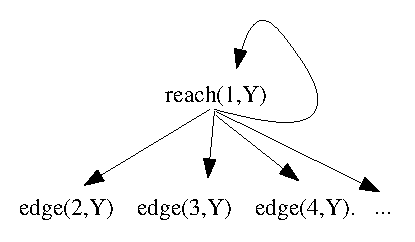
\includegraphics[width=\textwidth]{recursion}
%  \caption{Without \abstraction}
%  \label{fig:minipage1}
\end{minipage}
\quad
\begin{minipage}[b]{0.25\linewidth}
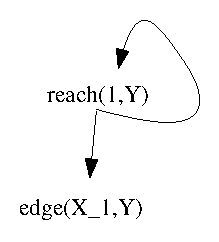
\includegraphics[width=0.5\textwidth]{abs-recursion}
%  \caption{With \abstraction}
%  \label{fig:minipage2}
\end{minipage}
\caption{A left-linear program and schematic IDGs: Left
  without IDG abstraction; Right: with
  IDG abstraction} \label{fig:abstraction}
\end{figure}
%------------------------------------------------------------
Abstracting the {\tt edge/2} predicate has subtle differences from
abstracting tabled subgoals.
%  The implementation of subgoal
%abstraction for tabled subgoals was described in~\cite{RigS13},
As mentioned, the {\tt edge/2} predicate of
Fig.~\ref{fig:abstraction} is not tabled.  Furthermore, the actual
{\tt edge/2} subgoal itself should not be abstracted to depth 0 since
losing the first argument instantiation would prevent the use of
indexing.  Rather, only the IDG's representation of the subgoal
should be abstracted.  Abstraction of dynamic code for
the IDG can be specified via the declaration:
\begin{center}
{\tt :-dynamic edge/2 as incremental, abstract(0)}.
\end{center}

In \version{} dynamic incremental code can be abstracted, but
incremental interned tries (Section~\ref{sec:incr-update-tries})
cannot be.  Also, currently only depth 0 abstraction is supported.

\subsection{Summary and Implementation Status}
%
When using incremental tabling an application will most commonly need
only the default transparent approach, although in special
circumstances eager updating may be desired.  The main design choices
are as usual what to table, and also what dynamic predicates or tries
should be made incremental.  In addition, performance optimizations
may be made through a mixture of subgoal abstraction and dynamic
predicate abstraction.  This optimization can be informed by use of
{\tt statistics/0} which includes summary information about the IDG,
or using the IDG inspection predicates of
Section~\ref{sec:incr-preds1} if more details is needed.

%Thus the user has four choices: tables may be
%updated as soon as the database is changed (e.g., via {\tt
%  incr\_assert/1}); at some point after a series of database changes
%(e.g. via {\tt incr\_assert\_inval/1} and {\tt
%  incr\_table\_update/0}); or lazily whenever a given table is called.
%In addition, if the changes are so massive that there is no point in
%incrementally updating the table, the tables can be abolished so that
%the tables will be reconstructed whenever they are re-queried.

In the current version of XSB, incremental tabling has not yet been
ported to the multi-threaded engine.  In addition, incremental tabling
only works for predicates that use both call and answer variance.
However, incremental tabling does work with for the full well-founded
semantics, for trie indexed dynamic code (in addition to regular
dynamic code) and with interned tries as described in
Section~\ref{sec:incr-update-tries}.  The space reclamation predicates
{\tt abolish\_all\_tables/0}, {\tt abolish\_table\_call/[1,2]} and
{\tt abolish\_table\_pred/[1,2]} can be safely used with incremental
tables.

\subsection{Predicates for Incremental Table Maintenance} \label{sec:incr-preds1}

\paragraph{A Note on Terminology}
%
Suppose {\tt p/1} and {\tt q/1} are incrementally tabled, and that
there is a clause
%
\begin{verbatim}
p(X):- q(X).
\end{verbatim}
%
In this case we say that {\tt p(X)} {\em depends\_on} {\tt q(X)} and
that {\tt q(X)} {\em affects} {\tt p(X)}.  A recursive predicate both
depends on and affects itself.


\paragraph{Declarations} The following directives support incremental
tabling based on changes in dynamic code: 

\index{tabling!opaque}
\index{tabling!declarations}
\begin{description}
\index{tabling!incremental}

\ourstandarditem{table +PredSpecs as incremental}{table/1}{Tabling}
%
is a executable predicate that indicates that each tabled predicate
specified in {\tt PredSpec} is to have its tables maintained
incrementally.  {\tt PredSpec} is a list of skeletons, i.e. open
terms, or {\tt Pred/Arity} specifications~\footnote{No explicit module
  references are allowed.}.  The tables must use call variance and
answer variance and must be compiled and loaded into the
single-threaded engine.  If a predicate is declared with tabling
attributes that are not supported with incremental tabling a
permission error is thrown.  This predicate implies that its arguments
are tabled predicates.  See page \pageref{table-declaration} for
further discussion of tabling options.

We also note that any tabled predicate that is called by a predicate
tabled as incremental must also be tabled as incremental or as opaque.
On the other hand, a dynamic predicate {\tt d/n} that is called by a
predicate tabled as incremental may or may not need to be declared as
incremental.  However if {\tt d/n} is not declared incremental, then
changes to it will not be propagated to incrementally maintained
tables.

\ourstandarditem{dynamic +PredSpecs as incremental}{dynamic/1}{Tabling}
%
is an executable predicate that indicates that each predicate in {\tt
  PredSpecs} is dynamic and used to define an incrementally tabled
predicate and will be updated using {\tt incr\_assert/1} and/or {\tt
  incr\_retractall/1} (or relatives.)  Note that dynamic incremental
predicates cannot themselves be tabled.  This predicate implies that
its arguments are dynamic predicates.  See page
\pageref{dynamic-declaration} for further discussion of dynamic
options.

\ourstandarditem{table +PredSpecs as opaque}{table/1}{Tabling} 
%
is an executable predicate that indicates that each predicate $P$ in
{\tt PredSpecs} is tabled and is used in the definition of some
incrementally tabled predicate but should not be maintained
incrementally.  In this case the system assumes that the programmer
will abolish tables for $P$ in such a way so that re-calling it will
always give semantically correct answers.  In other words, instead of
maintaining information to support incremental table maintenance, the
system re-calls the opaque predicate whenever its results are required
to recompute an answer.  One example of an appropriate use of opaque
is for tabled predicates in a DCG used to parse some string.  Rather
than incrementally maintain all dependencies on all input strings, the
user can declare these intermediate tables as opaque and abolish them
before any call to the DCG.  This predicate implies that its arguments
are tabled predicates.

\end{description}

\paragraph{Basic Incremental Maintenance Predicates}
The following predicates are used to manipulate incrementally
maintained tables:

\begin{description}
\ourrepeatmoditem{incr\_assert(+Clause)}{incr\_assert/1}{increval} 
\ourrepeatmoditem{incr\_assertz(+Clause)}{incr\_assertz/1}{increval}
\ourrepeatmoditem{incr\_asserta(+Clause)}{incr\_asserta/1}{increval}
\ourrepeatmoditem{incr\_retract(+Clause)}{incr\_retract/1}{increval}
\ourmoditem{incr\_retractall(+Term)}{incr\_retractall/1}{increval}
% 
are versions of {\tt assert/1} and other standard Prolog predicates.
They modify dymamic code just as their Prolog counterparts, but they
then invalidate all incrementally maintained tables that depend on
{\tt Clause}.

{\bf Error Cases} are the same as {\tt assert<a/z>/1}, {\tt retract/1}
and {\tt retractall/1} with the additional error condition:

\begin{itemize}
\item The head of the clause {\tt Clause} or the {\tt Term} refers to
  a predicate that is not incremental and dynamic.  
\bi
\item  {\tt type error(dynamic\_incremental, Term)}
\ei
\end{itemize}

\ourrepeatmoditem{incr\_assert\_update(+Clause)}{incr\_assert\_update/1}{increval}
\ourrepeatmoditem{incr\_assertz\_update(+Clause)}{incr\_assertz\_update/1}{increval}
\ourrepeatmoditem{incr\_asserta\_update(+Clause)}{incr\_asserta\_update/1}{increval}\
\ourrepeatmoditem{incr\_retractall\_update(+Clause)}{incr\_retractall\_update/1}{increval}
\ourmoditem{incr\_retract\_update(+Term)}{incr\_retract\_update/1}{increval}
%
are versions of {\tt assert/1} and other standard Prolog predicates.
They modify dymamic code just as their Prolog counterparts, mark any
incrementally maintained tables that depend on the modification as
invalid, then immediately update these tables.
%  The tables may be updated by an
%explicit call to {\tt incr\_table\_update/[0,1,2]}, or the table will
%be dynamically recomputed when a query is made to it.

\ourmoditem{incr\_table\_update}{incr\_table\_update/0}{increval} may
be called after base predicates have been changed (by {\tt
  incr\_assert/1} and/or {\tt incr\_retract/1} or friends).  This
predicate updates all the incrementally maintained tables whose
contents may be affected by those changes to the base predicates.
%This update operation is separated from the operations that change the
%base predicates ({\tt incr\_assert\_inval/1} and {\tt
%  incr\_retractall\_inval/1}) so that a set of base predicate changes
%can be processed all at once, which may be much more efficient that
%updating the tables at every base update.  Beginning with Version
%3.3.7, it is not absolutely necessary to call this predicate, as
%tables will be incrementally updated upon demand.  However, using this
%predicate allows a choice of incurring the cost of update at a time
%other than querying an updated goal.
Explicit update calls only need to be used in special circumstances
(cf. Section~\ref{sec:incr-eager}).

{\bf Error Cases}
\bi
\item A table $T$ that is to be incrementally updated is not yet
  complete.  
\bi
\item 	{\tt permission\_error(update, incomplete\_table Goal)}
\ei
\ei

\ourmoditem{incr\_table\_update(-GoalList)}{incr\_table\_update/1}{increval}
acts as {\tt incr\_table\_update/0} in its action to update the
incrementally maintained tables after changes to base predicates.  It
returns the list of goals whose tables were changed in the update
process.

\ourmoditem{incr\_table\_update(+SkelList,-GoalList)}{incr\_table\_update/2}{increval}
acts as {\tt incr\_table\_update/1} in its action to update
incrementally maintained tables after changes to base predicates.  The
first argument is a list of predicate skeletons (open terms) for
incrementally maintained tables.  The predicate returns in {\tt
  GoalList} a list of goals whose skeletons appear in {\tt SkelList}
and whose tables were changed in the update process.  In this way {\tt
  SkelList} acts as a filter to restrict the goals that are returned
to those of interest.  If {\tt SkelList} is a variable, all affected
goals are returned in {\tt GoalList}.

\ourmoditem{incr\_invalidate\_call(+Goal)}{incr\_invalidate\_call/1}{increval}
is used to directly invalidate a call to an incrementally maintained
table, {\tt Goal}.  A subsequent call to {\tt Goal} will automatically
perform incremental updating for {\tt Goal} along with any tables that
{\tt Goal} depends on that are in need of updating; similarly an
invocation of {\tt incr\_table\_update/[0,1,2]} will cause {\tt Goal}
to be recomputed along with all incrementally maintained tables that
{\tt Goal} affects.  This predicate can be used if a tabled predicate
depends on some external data and not (only) on dynamic incremental
predicates.  For example, if an incrementally maintained predicate
depends on a relation stored in an external relational database
(perhaps accessed through the ODBC interface), then this predicate can
be used to invalidate the table when the external relation changes.
The application programmer must know when the external relation
changes and invoke this predicate as necessary.

{\bf Error Cases}
\bi
\item 	{\tt Goal} is tabled, but not incrementally tabled
\bi
\item 	{\tt permission\_error(invalidate,non-incremental predicate,Goal)}
\ei
\ei

\end{description}

\paragraph{Incremental Maintenance using Interned Tries}
The following predicates are used to modify incremental tries, and can
be freely intermixed with predicates for modifying incremental dynamic
code, as well as with predicates for invalidating or updating tables
(Section~\ref{sec:incr-preds1}).

\begin{description}
\ourmoditem{incr\_trie\_intern(+TrieIdOrAlias,+Term)}{incr\_trie\_intern/2}{intern}
%
is a version of {\tt trie\_intern/2} for tries declared as
incremental.  A call to this predicate interns {\tt Term} in {\tt
  TrieIdOrAlias} and then invalidates all incrementally maintained
tables that depend on this trie.

\ourmoditem{incr\_trie\_uninternall(+TrieIdOrAlias,+Term)}{incr\_trie\_uninternall/2}{intern}
%
is a version of {\tt trie\_unintern/2} for tries declared as
incremental.  A call to this predicate removes all terms unifying with
{\tt Term} in {\tt TrieIdOrAlias} and then invalidates all
incrementally maintained tables that depend on this trie.

\ourmoditem{incr\_trie\_intern\_update(+TrieIdOrAlias,+Term)}
           {incr\_trie\_intern\_update/2}{intern}
%
works for tries declared as incremental in a similar manner as {\tt
  incr\_trie\_intern/2} except that it also immediatesly updates any
affected tables.

\ourmoditem{incr\_trie\_uninternall\_inval(+TrieIdOrAlias,+Term)}
{incr\_trie\_uninternall\_inval/2}{intern}
%
works for tries declared as incremental in a similar manner as {\tt
  incr\_trie\_uninternall/2} except that it also immediately updates
any affected tables.
\end{description}

\index{residual dependency graph}
\index{incremental dependency graph}
\paragraph{Inspecting Dependencies among Incremental Subgoals}
%
% These relations form a labelled directed graph for which the
%nodes are incrementally tabled subgoals present in XSB; a given
%subgoal in the graph may or may not have been completed.  
%Conceptually, there is an edge from $S_1$ to $S_2$ labelled depends
%(affects) if $S_1$ directly depends on (directly affects) $S_2$.  We
%call this graph the {\em incrementally tabled subgoal dependency
%  graph}, or just the incremental dependency graph.  
The predicates in this section allow a user to inspect properties of
IDG that can be useful in debugging, profiling or optimizing a
computation~\footnote{The predicates for traversing the incremental
  dependency graph are somewhat analogous to those for traversing the
  residual dependency graph (Section~\ref{sec:table-inspection}).}.

As explained below, IDG nodes can be accessed via the predicate {\tt
  is\_incremental\_subgoal/1}, while IDG edges can be accessed via
{\tt incr\_directly\_depends/2}.  The predicates {\tt
  get\_incr\_scc/[1,2]} and {\tt get\_incr\_scc\_with\_deps/[3,4]} can
be used to efficiently materialize the dependency graph in Prolog,
including SCC information.

\begin{description}

\ourmoditem{is\_incremental\_subgoal(?Subgoal)}{is\_incremental\_subgoal/1}{increval}
%
This predicate non-deterministically unifies {\tt Subgoal} with
incrementally tabled subgoals that are currently table entries.

\ourmoditem{incr\_directly\_depends(?Goal$_1$,?Goal$_2$)}{incr\_directly\_depends/2}{increval}
accesses the edges of the IDG: the incremental goals (Tables) that
directly depend on or directly affect one another.  At least one of
{\tt Goal$_1$} or {\tt Goal$_2$} must be bound.
\begin{itemize}
\item If {\tt Goal$_1$} is bound, then this predicate will return in
  {\tt Goal$_2$} through backtracking the goals for all incrementally
  maintained tables on which {\tt Goal$_1$} directly depends.
\item If {\tt Goal$_2$} is bound, then it returns in {\tt Goal$_1$}
  through backtracking the goals for all incrementally maintained
  tables that {\tt Goal$_2$} directly affects -- in other words all
  goals that directly depend on {\tt Goal$_2$}.  \ei

{\bf Error Cases}
\bi
\item Neither {\tt Goal$_1$} nor {\tt Goal$_2$} is bound 
\bi
\item 	{\tt instatiation\_error}
\ei
\item {\tt Goal$_1$} and/or {\tt Goal$_2$} is bound, but is not
  incrementally tabled
\bi
\item 	{\tt table\_error}
\ei
\ei

\ourmoditem{incr\_trans\_depends(?Goal$_1$,?Goal$_2$)}{incr\_trans\_depends/2}{increval}
is similar to {\tt incr\_directly\_depends/2} except that it returns
goals according to the transitive closure of the ``directly depends''
relation.  Error conditions are the same as {\tt
  incr\_directly\_depends/2}.

\ourrepeatmoditem{get\_incr\_sccs(?SCCList)}{get\_incr\_sccs/1}{increval}
\ourrepeatmoditem{get\_incr\_sccs\_with\_deps(?SCCList,?DepList)}{get\_incr\_sccs\_with\_deps/2}{increval}
\ourrepeatmoditem{get\_incr\_sccs(+SubgoalList,?SCCList)}{get\_incr\_sccs/2}{increval}
\ourmoditem{get\_incr\_sccs\_with\_deps(+SubgoalList,?SCCList,?DepList)}{get\_incr\_sccs\_with\_deps/3}{increval}
%
Most linear algorithms for SCC detection over a graph use destructive
assignment on a stack to maintain information about the connecteness
of a component; as a result such algorithms are
difficult to write efficiently in Prolog.

{\tt get\_incr\_sccs/1} unifies {\tt SCCList} with SCC information for
the incremental dependency graph that is represented as a list whose
elements are of the form
\begin{center}
{\tt ret(Subgoal,SCC)}.
\end{center}
{\tt SCC} is a numerical index for the SCCs of Subgoal. Two subgoals
are in the same SCC iff they have the same index, however no other
dependency information can be otherwise directly inferred from the
index~\footnote{The actual number for each SCC index depends on how
  the incremental dependency graph happens to be traversed; as a
  result it is best to rely on the index only as a ``generated'' name
  for each SCC.}.

If dependency information is also desired, {\tt
  get\_incr\_scc\_with\_dependencies/2} should be called.  In addition
to the SCC information as above, {\tt DepList} is unified with a list
of dependency terms of the form
\begin{center}
{\tt depends(SCC1,SCC2)}
\end{center}
for each pair {\tt SCC1} and {\tt SCC1} such that some subgoal with
index {\tt SCC1} directly depends on some subgoal with index {\tt
  SCC1}.  If it is necessary to know which subgoal(s) in {\tt SCC1}
directly depends on which subgoal(s) in {\tt SCC2}, the information
can be easily reconstructed using {\tt incr\_directly\_depends/2}
above.  Similarly, {\tt incr\_directly\_depends/2} can be used to
determine the actual edges within a given SCC.

Ordinarily a user will want to see the entire dependency graph and in
such a case the predicates described above should be used.  However,
note that if the dependency graph is the result of several
indepdendent queries it may not be connected.  {\tt get\_incr\_scc/2}
takes as input a list of incremental subgoals, {\tt SubgoalList}.  For
each {\tt Subgoal} in {\tt SubgoalList}, this predicate finds the set
of subgoals connected to {\tt Subgoal} by any mixture of depends and
affects relations, unions these sets together, and finds the SCCs of
all subgoals in the unioned set.

SCC detection is implemented using Tarjan's algorithm~\cite{Tarj72} in
C working directly on XSB's data structures.  The algorithm is
$\cO(|V| + |E|)$ where $|V|$ is the number of vertices and $|E|$ the
number of edges in the dependency graph.  As a result, {\tt
  get\_incr\_sccs/[1,2]} provides an efficient means to materialize the
  high-level topography of the dependency graph~\footnote{Currently,
    the materialization of dependency information between SCCs is
    implemented in a naive manner, so that {\tt
      get\_incr\_sccs\_with\_deps/[2,3]} is $\cO(|V|^2)$.}.

{\bf Error Cases}
\bi
\item {\tt SCCList} contains a predicate that is not tabled
\bi
\item 	{\tt permission\_error}
\ei
\ei
\end{description}


%--------------------------------------------------------------------

\section{A Weaker Semantics for Tabling}
%
\index{completion semantics}
\index{completion semantics!weak}
Recall that the well-founded semantics (WFS) is weaker than, say,
the Stable model semantics.  For instance a program like
%
\begin{verbatim}
p:- not q.            q:- not p.
\end{verbatim}
%
has two stable models: $\{p\}$ and $\{q\}$.  On the other hand, WFS
has a single model, where both $p$ and $q$ are undefined.  This, of
course, is characteristic of the way WFS treats atoms whose only
non-failed derivations are based on a ``negative loop''.

However, an even weaker logic is possible where derivations based on
positive loops are also considered undefined.  In other words the
program
\begin{verbatim}
   r:- r.                r:- false.
\end{verbatim}
would assign the truth value {\em undefined} to $r$, although both WFS
and stable models would assign r as {\em false}.  But why use such a
weak logic?

Consider a woman who asks her husband when he'll clean the garage, and
the husband says:

{\em I'll get around to it when I get around to it.}

The wife would probably consider it ambiguous not only when her
husband might clean the garage, but whether he would do so at all.
The wife's reasoning (slightly simplified) could be rendered in logic
as:

\begin{verbatim}
   clean_the_garage:- clean the garage.
\end{verbatim}
\noindent
and we'd like to assign {\em undefined} or {\em unknown} to {\tt
  clean\_the\_garage}.\footnote{Actually, many wives would go ahead
  and assign {\em false} to this statement, but we are modeling an
  optimistic (or possibly delusional) wife.}

Although this example is somewhat fanciful, it turns out that this
interpretation accords with the results of cognitive science
experiments about human reasoning~\cite{SteV08}, and is known in the
logic programming community as the ``completion semantics'' (CS).  CS
differs from WFS only in assigning the truth value {\em undefined} to
derivations that depend on a positive loop, and that are otherwise not
satisfiable (cf. \cite{Lloy84}).

%Thus, in this
%new semantics positive loops are treated in an analogous way to
%negative loops.Formally, the new semantics can be expressed as a fixed
%point logic based on Clark's completion semantics~\cite{??}, when
%logical expressions are satisfied according to the Lukasiewicz
%3-valued semantics for propositional programs, which is weaker than
%some other approaches to 3-valued satisfiability, namely that of
%Kleene (see \cite{??}).  However, this level of formality is not
%necessary as long as one understands how positive and negative loops
%are evaluated.  We call this semantics the {\em completion semantics
%  (CS)}.

So as useful as WFS and stable models are for programming, they don't
reflect how human beings have been shown to reason in daily life.
However, there is another difference between WFS and the sort of
common-sense reasoning that humans perform.  WFS has a strong {\em
  closed-world} assumption.  Suppose a query {\tt ?- s} were made to a
program where {\tt s} were not defined.  WFS would assign the value
{\em false} to {\tt s}, but this is not always what humans do: rather
humans would treat the unknown predicate {\tt s} as in fact {\em
  unknown} or {\em undefined}.  More generally, if (sub-)goal $G$
refers to an undefined predcate,the {\em weak} completion semantics
(WCS) also assigns {\em undefined} to $G$, rather than {\em false} as
WFS does, or throwing an error (as XSB also does by default).

\begin{itemize}
\item For one or more tabled predicates ro use the comploetion semantics,
use the declaration

\noindent
{\tt \mif{} table {\em PredSpec} as compl\_semantics.}

\item Setting the ISO Prolog flag {\tt unknown} to {\tt undefined}
  makes calls to unknown predicates return the truth value {\em
    undefined}.  E.g., 
\begin{verbatim}
?- set_prolog_flag(unknown,undefined).
\end{verbatim}
This flag can also be set to the standard ISO values,
  {\tt fail}. {\tt warning} or {\tt error} (the last of which is the
    default).

\item The various forms of tabled negation work well with the
  completion semantics; however if mixing tabled and non-tabled
  predicates it is best to use {\tt not3/1} (cf. pg. \pageref{not3})
  rather than the SLD operators {\tt not/1} or \verb|\+/1|.
\end{itemize}

%\noindent
%These features can be set globally either separately or together:

%\begin{itemize}
%\item \item Setting the Prolog flag {\tt alt\_semantics} to {\tt cs} causes
%  XSB to globally evaluate the completion semantics.
%\item Setting the Prolog flag {\tt alt\_semantics} to {\tt weak\_cs} causes
%  XSB to globally evaluate the weak completion semantics, and is
%  equivalent to setting the {\tt alt\_semantics} flag to {\tt cs} and
%  the ISO flag {\tt unknown} to {\tt undefined}.
%\item Setting the Prolog flag {\tt alt\_semantics} to {\tt wfs} turns
%  causes XSB to behave in its default mode.  I.e., to globally
%  evaluate queries according to the well-founded semantics, and to
%  throw an error when encountering an unknown predicate.
%\end{itemize}

(W)CS and WFS can be mixed on a per-predicate basis.  If a goal
$G_{WFS}$ to a predicate declared to use WFS is involved in a loop
with a goal $G_{CS}$ declared to use CS, then $G_{WFS}$ is evaluated
according to the (W)CS.

\paragraph{Examples}

As a simple example, consider the program:
\begin{verbatim}
:- table simple_loop/1 as compl_semantics.
simple_loop(X):- simple_loop(X).     simple_loop(X):- p(X).
p(a).
\end{verbatim}
The query {\tt ?- simple\_loop(X)} returns two answers: {\tt X = a} as
{\em true}, and {\tt X} unbound as {\em undefined}.

For a more complex example, consider the program:
\begin{verbatim}
:- table m_1_1/1,m_1_2/1,m_1_3/1,m_1_4/1 as compl_semantics.
m_1_1(X):- m_1_2(X).         m_1_1(a):- m_1_2(a).
m_1_2(X):- m_1_3(X).         m_1_2(a):- m_1_3(a).         
m_1_3(X):- m_1_4(X),fail.    m_1_3(a):- m_1_4(a).
m_1_4(X):- m_1_1(X).         m_1_4(a):- m_1_1(a).
\end{verbatim}
%
The derivation of the query {\tt ?- m\_1\_1(X)} creates a positive SCC
with with numerous interrelated positive cycles, but these cycles can
be broken down into two groups.  The first group includes a dependency
edge from {\tt m\_1\_3(X)} to {\tt m\_1\_4(X)}, while the other set
does not include this edge.  Due to the first clause of {\tt
  m\_1\_3(X)}, all derivations in the first group fails, although
derivations that do not include this edge succeed.  Thus the only
answer to {\tt m\_1\_1(X)} has {\tt X = a} with truth value {\em
  undefined} (and a single delay list of {\tt [m\_1\_2(a)]}.


\index{tabling!call subsumption}
\index{tabling!call variance}
\index{tabling!answer subsumption}
\index{tabling!incremental}

\section{Compatibility of Tabling Modes and Predicate Attributes} \label{sec:tabling-compatibility}
%
As discussed in this chapter, there are several choices for how to
table a predicate. Either call subsumption or call variance may be
used, incremental tabling might or might not be used, and answer
subsumption might or might not be used.  Ground terms may be interned.
Furthermore, a tabled predicate, like any other predicate, may be
static or dynamic and thread shared or thread private.  Additionally
various abstraction methods may be used, such as subgoal abstraction,
answer abstraction, or maximal answers.  And finally, a tabled
predicate may be declared as private or shared in the multi-threaded
engine.  

To analyze further, all combinations are supported for call-variance
and for thread private predicates.  However, call subsumption has not
been fully integrated with dynamic code or thread shared predicates,
and cannot currently be combined with incremental tabling or with
answer subumption.  Similarly incremental tabling is not yet supported
in the multi-threaded engine (it is supported for ``thread private''
computations only in the sequential engine).  The compatibilities are
listed in Table~\ref{table:table}.  Further combinations will be
supported in future versions of XSB as resources allow.

The combinations in Table~\ref{table:table} allow full well-founded
computation, constrained variables in calls and answers (including the
residual program), and safe space reclamation, with the following
exceptions.  Answer subsumption does support non lrd-stratified
programs; and call subsumption does not yet support attributed
variables in calls.  \index{attributed variables}

\begin{itemize}
\item A predicate $P$ declared with {\tt ans\_subsumption} cannot also
  be declared with {\tt answer abstract, compl\_semantics, dynamic, incremental, intern,
    opaque, subgoal\_abstract} or {\tt subsumptive}.
%
\item A predicate $P$ declared with {\tt answer\_abstract} cannot also
  be declared with {\tt ans\_subsumption, intern} or {\tt
    compl\_semantics}.
%
\item A predicate $P$ declared with {\tt compl\_semantics} cannot also
  be declared with {\tt ans\_subsumption, answer\_abstract, dynamic,
    incremental, intern, opaque, subsumptive} or {\tt subgoal\_abstract}.
%
\item A predicate $P$ declared with {\tt dyn} or {\tt (dynamic)} cannot also
  be declared with {\tt ans\_subsumption} or {\tt incremental}
%
\item A predicate $P$ declared with {\tt incremental} cannot also be
  declared with {\tt compl\_semantics, dynamic, intern,
    nonincremental, opaque, shared} or {\tt subsumptive}.  However,
  $P$ may be changed from {\tt incremental} to {\tt nonincremental} or
  {\tt opaque} via {\tt set\_predicate\_property/2}.
%
\item A predicate $P$ declared with {\tt intern} cannot also be
  declared with {\tt ans\_subsumption, answer\_abstract,
    compl\_semantics, incremental, subgoal\_abstract} {\tt subsumption}
  intern,Options,PredCList).
%
\item A predicate $P$ declared with {\tt max\_answers} cannot also be
  declared with {\tt compl\_semantics} or {\tt subsumptive}.
%
\item A predicate $P$ declared with {\tt nonincremental} cannot also
  be declared with {\tt incremental} or {\tt opaque}.  However, $P$
  may be changed from {\tt nonincremental} to {\tt incremental} or
  {\tt opaque} via {\tt set\_predicate\_property/2}.
%
\item A predicate $P$ declared with {\tt opaque} cannot also be
  declared with {\tt incremental} or {\tt nonincremental}.  However,
  $P$ may be changed from {\tt opaque} to {\tt nonincremental} or {\tt
    incremental} via {\tt set\_predicate\_property/2}.
%
\item A predicate $P$ declared with {\tt private} cannot also
  be declared with {\tt shared}.
%
\item A predicate $P$ declared with {\tt shared} cannot also be
  declared with {\tt compl\_semantics, incremental, opaque, private}
  or {\tt subsumptive}.
%
\item A predicate $P$ declared with {\tt subgoal\_abstract} cannot also
  be declared with {\tt subsumptive}.
%
\item A predicate $P$ declared with {\tt subsumptive} cannot also be
  declared with {\tt compl\_semantics, max\_answers, shared} or {\tt
    subgoal\_abstract}.  However, $P$ may be changed from {\tt
    subsumptive} to {\tt variant} via {\tt
    set\_predicate\_property/2}.
%
\item A predicate $P$ declared with {\tt variant} cannot also be
  declared with {\tt subsumptive}. However, $P$ may be changed from
  {\tt variant} to {\tt subsumptive} via {\tt
    set\_predicate\_property/2}.

\end{itemize}

%\begin{table}
%\begin{center}
%{\footnotesize
%\begin{tabular}{llllll}\hline \hline
%%variant/subsumptive & dynamic/static & shared/private & incremental/opaque  & answer subsumption  \\
%variant &	    static & 	   private &	  nonincremental &      no answer subsumption  &  yes \\
%%variant &	    static &	   private &	  nonincremental &      answer subsumption     &  yes \\
%variant	&	    static &	   private &      opaque &             no answer subsumption  &  yes \\
%variant &	    static &	   private &	  opaque &	      answer subsumption &	no \\
%variant &	    static &	   private &	  incremental &         no answer subsumption &	yes \\
%variant &	    static &	   private &      incremental &         answer subsumption &	no \\
%variant &	    static &	   shared &	  nonincremental &      no answer subsumption &	yes \\
%variant &	    static &	   shared &	  nonincremental &      answer subsumption &	yes \\
%variant &	    static &	   shared &	  opaque &	      no answer subsumption &	no \\
%variant &	    static &	   shared &	  opaque &	      answer subsumption &	no \\
%variant &	    static &	   shared &	  incremental &       no answer subsumption &	no \\
%variant &	    static &	   shared &	  incremental &          answer subsumption &	no \\
%variant &	    dynamic &	   private &	  nonincremental &      no answer subsumption &	yes \\
%ariant &	    dynamic &	   private &	  nonincremental &      answer subsumption &	yes \\
%variant &	    dynamic &	   private &	  opaque &	      no answer subsumption &	no \\
%variant &	    dynamic &	   private &	  opaque &	      answer subsumption &	no \\
%variant &	    dynamic &	   private &	  incremental &         no answer subsumption &	no \\
%%variant &	    dynamic &	   private &	  incremental &         answer subsumption &	no \\
%variant &	    dynamic &	   shared &	  nonincremental &      no answer subsumption &	yes \\
%variant &	    dynamic &	   shared &	  nonincremental &      answer subsumption &	yes \\
%variant &	    dynamic &	   shared &	  opaque &	      no answer subsumption &	no \\
%variant &	    dynamic &	   shared &	  opaque &	      answer subsumption &	no \\
%variant &	    dynamic &	   shared &	  incremental &         no answer subsumption &	no \\
%variant &	    dynamic &	   shared &	  incremental &         answer subsumption &	no \\
%subsumptive &	    static &	   private &	  nonincremental &      no answer subsumption &	yes \\
%subsumptive &	    static &	   private &	  nonincremental &      answer subsumption &	yes \\
%subsumptive &	    static &	   private &	  opaque &	      no answer subsumption &	no \\
%subsumptive &	    static &	   private &	  opaque &	      answer subsumption &	no \\
%subsumptive &	    static &	   private &	  incremental &         no answer subsumption &	no \\
%subsumptive &	    static &	   private &	  incremental &         answer subsumption &	no \\
%subsumptive &	    static &	   shared &	  nonincremental &      no answer subsumption &	no \\
%subsumptive &	    static &	   shared &	  nonincremental &      answer subsumption &	no \\
%subsumptive &	    static &	   shared &	  opaque &	      no answer subsumption &	no \\
%subsumptive &	    static &	   shared &	  opaque &	      answer subsumption &	no \\
%subsumptive &	    static &	   shared &	  incremental &       no answer subsumption &	no \\
%subsumptive &	    static &	   shared &	  incremental &          answer subsumption &	no \\
%subsumptive &	    dynamic &	   private &	  nonincremental &      no answer subsumption &	yes \\
%subsumptive &	    dynamic &	   private &	  nonincremental &      answer subsumption &	yes \\
%subsumptive &	    dynamic &	   private &	  opaque &	      no answer subsumption &	no \\
%subsumptive &	    dynamic &	   private &	  opaque &	      answer subsumption &	no \\
%subsumptive &	    dynamic &	   private &	  incremental &         no answer subsumption &	no \\
%subsumptive &	    dynamic &	   private &   	  incremental &         answer subsumption &	no \\
%subsumptive &	    dynamic &	   shared &	  nonincremental &      no answer subsumption &	no \\
%subsumptive &	    dynamic &	   shared &	  nonincremental &      answer subsumption &	no \\
%subsumptive &	    dynamic &	   shared &	  opaque &	      no answer subsumption &	no \\
%subsumptive &	    dynamic &	   shared &	  opaque &	      answer subsumption &	no \\
%subsumptive &	    dynamic &	   shared &	  incremental &         no answer subsumption &	no \\
%subsumptive &  	    dynamic &	   shared &	  incremental &         answer subsumption &	no \\ \hline \hline 
%\end{tabular}
%}
%\end{center}
%\caption{Support for different tabling modes in XSB \version}
%\label{table:table}
%\end{table}


%\section{Incremental Table Maintenance} \label{sec:incremental_tabling}
%====================================================

\index{tabling!incremental}

XSB allows the user to declare that the system should maintain the
correctness of a given table with respect to dynamically changing
facts and rules through so-called {\em incremental
  tables}~\cite{SaRa05,Saha06,Swif14}.
%A table $T$ is {\em incremental} if XSB ensures that its answers are
%  consistent with all dynamic facts and rules upon which $T$ depends
%  (subject to transactionality conditions explained below).
After a database update or series of updates $\Delta$, an incremental
table $T$ that depends on $\Delta$ is by default updated
transparently: that is $T$ and all tables upon which $T$ depends are
automatically updated (if needed) whenever a future subgoal calls $T$.
Alternately, if circumstances require it, a table can be updated
immediately upon a database change or by issuing an explicit command
to update all tables that depend on $\Delta$.
%
In either case, incremental tabling brings XSB closer to the
functionality of deductive databases.  If tables are thought of as
materialized database views (or snapshots), then the incremental table
maintenance subsystem enables incremental view maintenance; also as
discussed below, if choice points are thought of as database cursors
then incremental tabling also provides view consistency~\footnote{In
  the current version of XSB, there are certain restrictions on how
  incremental tabling can be used:
  cf. Section~\ref{sec:tabling-compatibility}.}.

\subsection{Transparent Incremental Tabling} \label{sec:incr_examples}

To demonstrate incremental table maintenance (informally called {\em
  incremental tabling}), consider first the following simple program
that does not use incremental tabling:
\begin{verbatim}
:- table p/2.
p(X,Y) :- q(X,Y),Y =< 5.

:- dynamic q/2.
q(a,1).    q(b,3).   q(c,5).    q(d,7).
\end{verbatim}
and the following queries and results:
\begin{verbatim}
| ?- p(X,Y),writeln([X,Y]),fail.
[c,5]
[b,3]
[a,1]

no
| ?- assert(q(d,4)).

yes
| ?- p(X,Y),writeln([X,Y]),fail.
[c,5]
[b,3]
[a,1]

no
\end{verbatim}
%
In this program, the table for {\tt p/2} depends on the contents of
the dynamic predicate {\tt q/2}.  We first evaluate a query, {\tt
  p(X,Y)}, which creates a table.  Then we use {\tt assert/1} to add a
fact to the {\tt q/2} predicate and re-evaluate the query.  We see
that the answers haven't changed, because the table is already created
and the second query just retrieves answers directly from that
existing table.  However the answers are inconsistent with the model
of {\tt p/2} after the assert.  I.e., if the table didn't exist
(e.g. if {\tt p/2} weren't tabled), the answer {\tt [d,4]} would also
be derived.  Without incremental table maintenance, the only solution
to this problem is for the XSB programmer to explicitly abolish a
table whenever changing (with assert or retract) a predicate on which
the table depends.
%
By declaring that the tables for {\tt p/2} should be incrementally
maintained, XSB automatically keeps the tables for {\tt p/2} correct.

%
Consider a slight rewrite of the above program:
\begin{verbatim}
:- table p/2 as incremental.
p(X,Y) :- q(X,Y),Y =< 5.

:- dynamic q/2 as incremental.
q(a,1).    q(b,3).    q(c,5).     q(d,7).
\end{verbatim}
in which {\tt p/2} is declared to be incrementally tabled
% (with {\tt  :- table p/2 as incremental}) 
and {\tt q/2} is declared to be both dynamic and incremental, meaning
that an incremental table depends on it.
%~\footnote{The declarations {\tt use\_incremental\_tabling/1} and
%  {\tt use\_incremental\_dynamic/1} are deprecated from Version 3.3 of
%  XSB forward -- in other words backwards compatibility will be
%  maintained for a time, but these declarations will not be further
%  supported.}.  
Consider the following goals and execution:
\begin{verbatim}
| ?- import incr_assert/1 from increval.
yes
| ?- p(X,Y),writeln([X,Y]),fail.
[c,5]
[b,3]
[a,1]

no
| ?- incr_assert(q(d,4)).

yes
| ?- p(X,Y),writeln([X,Y]),fail.
[d,4]
[c,5]
[b,3]
[a,1]

no
\end{verbatim}
\noindent
The transparent approach to incremental updating works as follows.
When {\tt incr\_assert/1} is called, it sparks an invalidation
phase in which tables that depend on {\tt q(d,4)} are marked as {\em
  invalid} (i.e., possibly inconsistent with respect to underlying
dynamic code).  An {\em Incremental Dependency Graph (IDG)} is used to
obtain the right tables to invalidate.  However, if the invalidation
phase finds an affected table that is incomplete, a permission error
is thrown, since it is unclear whether sensible semantics can be given
to updating a subgoal that is incomplete.  After the invalidation
phase is completed, when/if a subgoal calls an invalid table $T$ the
engine interrupts itself to recompute $T$ and any tables upon which
$T$ depends.  On the other hand, if no calls are ever made to an
invalid incremental table $T'$, $T'$ will never incur the cost of an
update.

\subsubsection{View Consistency} \label{sec:view-consistency}
%
As described above, transparent incremental tablings's use of lazy
updating ensures that a new query $Q$ will always be consistent with
the state of the dynamic code at the time $Q$ is called.  However,
transparent incremental tabling enforces a stronger property of view
consistency similar to those of database systems: that answers to a
query $Q$ should be those derivable at the time $Q$ was called, {\em
  and should not be affected by any updates}.
%Accordingly, the ISO standard for Prolog~\cite{ISO-Prolog} specifies
%that an update $\upsilon$ to dynamic code should not affect the
%behavior of choice points that were created before $\upsilon$.
Because XSB's incremental tabling does not allow updates that affect
tables that are still being computed, supporting view consistency
effectively means ensuring consistency for choice points into
completed incremental tables.  As such choice points correspond to
database cursors, we term them {\em Open Cursor Choice Points,
  (OCCPs)}.

XSB's support for view consistency is designed so that no perceptable
overhead in incurred if there are no OCCPs whose view needs to be
maintained.  Not surprisingly, numerous long-lived OCCPs whose views
need to be maintained across updates causes an overhead for the
engine, a situation that is in some sense similar to the cost of
maintaining views for cursors in database system.

%----------------------------------------------------------------
\comment{
In addition to the success continuations that are standard in most
languages, Prolog has failure continuations -- choice points to take
upon backtracking.  The presence of these failure continuations leads
to an issue of view consistency, even within a single-threaded
computation.  Suppose that a user
%
\begin{enumerate}
\item Makes a query to a completed incrementally tabled subgoal $Q$.
  $Q$ has more than one solution and the first one is returned,
  leaving a choice point into the table for $Q$.
\item Makes an update to dynamic code upon which $Q$ depends
\item Makes another query to $Q$
\end{enumerate}
%
What is the relation between the queries and the update.  Presumably,
the first query in step 1) should not reflect the changes made in step
2) if a user backtracks for further answers to that query -- this can
be seen as ensuring view consistency.. However it is less clear
whether the second query to $Q$ in step 4) should return the same
answers as the first query in step 1), or whether the second query
should reflect the database update.  Arguments can be made for either
approach.
%
\begin{itemize}
\item {\em Prolog-style semantics} If the second query reflects the
  database change, it is consistent with the database, but is not
  consistent with the first query~\footnote{This approach could be
    viewed as an extension of the ISO semantics for dynamic code in
    Prolog, which XSB does not currently support.};
\item {\em Delayed update semantics} If the second query does not
  reflect the dynamic code change, it is consistent with the first
  query but not with the dynamic code change.
\end{itemize}
%
XSB chooses the latter of these approaches.  If a user has failure
continuations into a query $Q$, then $Q$ and all tables that depend on
$Q$ will not be updated until these failure continuations have been
exhausted or removed.  However, all updates are ensured to be applied
once this is the failure continuations are removed.
}

%----------------------------------------------------------------

\subsection{Updating in a Three-Valued Logic}
%
As discussed earlier in this chapter, answers that are undefined in
the well-founded semantics are represented as conditional answers.
Beginning with version 3.3.7, incremental updates work correctly with
conditional answers~\footnote{Before Version 3.3.7, incremental
  updates only worked correctly on stratified tables: those with only
  unconditional answers.}.  Nno special care needs to be taken for
updating in the well-founded semantics as the following example
illustrates.
%conditional answers, and they can be updated through any of the
%previously described methods.  The following example illustrates one
%such approach.

\begin{verbatim}
:- dynamic data/1 as incremental.

:- table opaque_undef/0 as opaque.
opaque_undef:- tnot(opaque_undef).

:- table p/1 as incremental.
p(_X):- opaque_undef.
p(X):- data(X).
\end{verbatim}
%
Note that {\tt opaque\_undef/1} upon which {\tt p/1} depends is
explicitly declared as opaque~\footnote{An {\em opaque} predicate $P$
  is tabled and is used in the definition of some incrementally tabled
  predicate but should not be maintained incrementally.  In this case
  the system assumes that the programmer will abolish tables for $P$
  in such a way so that re-calling it will always give semantically
  correct answers.}.  When the above program is loaded, XSB will
behave as follows.
%
{\small
\begin{verbatim}
| ?- p1(1).

undefined
| ?- incr_assert(data(1)).

yes
| ?- p1(1).

yes
| ?- incr_retract(data(1)).

yes
| ?- p1(1).

undefined
| ?- get_residual(p1(1),C).

C = [opaque_undef]
\end{verbatim}
}
%

\subsection{Eager Incremental Tabling}~\label{sec:incr-eager}
%
Despite the advantages of transparent incremental tabling, there are
special circumstances when it may be better to update tables eagerly
rather than when (and if) they are called.  For instance, if updates
and queries are expected to occur at different times, performing eager
updates may improve query time.  In addition, if incremental tables
are accessed via table inspection predicates
(cf. Chapter~\ref{sec:TablingPredicates}) rather than by queries,
inconsistent answers may be obtained.  

\paragraph{An Eager Updating Approach}
%
Usually, best way to eagerly update tables is to use the {\tt
  incr\_assert/1} and {\tt incr\_retract(all)/1}
predicates as discussed above.  When the updates are finished, the
command {\tt incr\_table\_update/0} is then called, which updates all
tables that depend on any changed dynamic rules or facts.  The
following execution for our running program shows an example of this.

\begin{verbatim}
| ?- import incr_assert/1, incr_table_update/0 from increval.

yes
| ?- p(X,Y),writeln([X,Y]),fail.
[c,5]
[b,3]
[a,1]

no
| ?- incr_assert(q(d,4)), incr_assert(q(d,1)), 

yes
| ?- incr_table_update.

| ?- p(X,Y),writeln([X,Y]),fail.
[d,4]
[d,1]
[c,5]
[b,3]
[a,1]

no
\end{verbatim}
\noindent
As discussed, calling {\tt incr\_table\_update} causes the cost of
updating incremental tables to be immediately incurred, and ensures
that table inspection primitives show correct results.  However,
tables are updated and their views preserved even if the tables may
not be accessed before further updates are made.

\subsubsection{An Immediate Approach}
%
A final approach is to use the predicates {\tt incr\_assert\_update/1}
and {\tt incr\_retract(all)\_update/1}, which force immedidate updates
of invalidated tables.  While simple, this approach should only be
used in special circumstances, as calling {\tt incr\_assert\_update/1}
twice could cause tables to be updated twice rather than once.

\comment{
 We note, however, that the use of these predicates is much
less common than direct queries to tables; but if using table
inspection predicates on incrementally maintained tables, the user
should ensure that the tables have been eagerly updated as described
below in Section~\ref{}.  should ensure that {\tt
  incr\_table\_update/0} is called before inspecting the tables.

Here again we call {\tt p(X,Y)} and generate a table for it and its
answers.  Then we update {\tt q/2} by using the incremental version of
assert, {\tt incr\_assert/1}, which was explicitly imported.  Now when
we call {\tt p(X,Y)} again, the table has been updated and we get the
correct answer.

In this case after every {\tt incr\_assert/1} and/or {\tt
  incr\_retract(all)/1}, the tables are incrementally updated to
reflect the change.  The system keeps track of what tabled goals
depend on what other tabled goals and (incremental) dynamic goals, and
tries to minimize the amount of recomputation necessary.
Incrementally tabled predicates may depend on other tabled predicates.
In this case, those tabled predicates must also be declared as
incremental (or opaque).The algorithm used is described
in~
}
\subsubsection{Declaring Predicates to be Incremental}
%
In XSB, tables can have numerous properties: such as {\em subsumptive,
  variant, incremental, opaque, dynamic, private}, and {\em shared},
and can use answer subsumption or call abstraction.  XSB also has
variations in forms of dynamic predicates: {\em tabled, incremental,
  private}, and {\em shared}.  XSB extends the {\tt table} and {\tt
  dynamic} compiler and executable directives with modifiers that
allow users to indicate the kind of tabled or dynamic predicate they
want.  For example,
%
\begin{verbatim}
:- table p/3,s/1 as subsumptive,private.

:- table q/3 as incremental,variant.

:- dynamic r/2,t/1 as incremental.
\end{verbatim}
%We note that
%\begin{verbatim}
%:- table p/3 as dyn.
%and
%:- dynamic p/3 as tabled.
%\end{verbatim}
%are equivalent.

In the current version of XSB, incremental tabling works with subgoal
abstraction, answer abstraction, and well-founded negation.  However
several combinations involving incremental tabling are not supported
and will throw an error (cf. page \pageref{table-declaration} and page
\pageref{dynamic-declaration}, respectively). Incremental tabling has
not yet been ported to the multi-threaded engine and and it currently
works only for predicates that use both call and answer variance.

\index{tries!and incremental tabling}
\subsection{Incremental Tabling using Interned Tries} \label{sec:incr-update-tries}
%
Sometimes it is more convenient or efficient to maintain facts in
interned tries rather than as dynamically asserted facts
(cf. Chapter~\ref{chap:tries}).  Tables based on interned tries can be
automatically updated when terms are interned or uninterned just as
they can be automatically updated when a fact is asserted or
retracted.  Consider the example from Section~\ref{sec:incr_examples}
rewritten to use interned tries.  As usual, an incrementally updated
table is declared as such:
%
\begin{verbatim}
:- table p/2 as incremental.
p(X,Y) :- trie_interned(q(X,Y),inctrie),Y =< 5.
\end{verbatim}
%
However, the declaration for dynamic data changes: rather than using
the declaration 
\begin{center}
{\tt :- dynamic q/2 as incremental}
\end{center}
a trie is specified as incremental in its creation.
%
\begin{center}
{\tt  trie\_create(Trie\_handle,[incremental,alias(inctrie)])}
\end{center}
%
As described in Chapter~\ref{chap:tries}, the trie handle returned is
an integer, but can be aliased just as with any other trie.  The trie
may then be initially loaded:
%
\begin{verbatim}
	trie_intern(q(a,1),inctrie),trie_intern(q(b,3),inctrie),
	trie_intern(q(c,5),inctrie),trie_intern(q(d,7),inctrie).
\end{verbatim}
%
At this stage a query to {\tt p/2} acts as before:
%
\begin{verbatim}
| ?- p(X,Y),writeln([X,Y]),fail.
[c,5]
[b,3]
[a,1]
\end{verbatim}
%
The following sequence ensures that {\tt p/2} is incrementally updated
as {\tt inctrie} changes:
%
\begin{verbatim}
| ?- import incr_trie_intern/2.

yes
| ?- incr_trie_intern(inctrie,q(d,4)).

yes
| ?- p(X,Y),writeln([X,Y]),fail.
[d,4]
[c,5]
[b,3]
[a,1]

no
\end{verbatim}
%
Given the proper directives to make a trie incremental, transparent
incremental tabling works for changes made to interned tries just as
it does for regular dynamic code and for trie-indexed dynamic code.
There are also the predicates {\tt incr\_trie\_intern\_update/2} and
{\tt incr\_trie\_unintern\_updatesl/2} which immediately update
dependent tables.

\index{Incremental Dependency Graph (IDG)}
\subsection{Abstracting the IDG for Better Performance} \label{sec:IDG-abs}
As mentioned above, incremental table mantenance makes use of an IDG.
Specifically, the nodes of the IDG are the incrementally tabled
subgoals; and each such table contains information about its incident
edges: those subgoals upon which a node directly depends or directly
affects.  While the IDG is a critical data structure to efficiently
update incremental tables, in certain situations constructing the IDG
can cause non-trivial overheads in query time and table space.  These
overheads can be addressed in many cases by {\em abstracting} the IDG.
When a tabled subgoal $S$ is called, rather than creating an edge
between $S$ and its nearest tabled ancestor $S'$ (if any), one could
abstract $S$, $S'$ or both, potentially collapsing a large number of
nodes and edges of the IDG.  If $S$ is an incremental table, then
performing subgoal abstraction on $S$ as introduced in
Section~\ref{sec:tabling-termination}, will abstract the IDG -- rather
than having $n$ nodes $S_1,\ldots,S_n$ and their associated links, the
IDG will contain a single node $abstract(S)$.  However, subgoal
abstraction will not work to abstract the leaf nodes of the IDG, which
are subgoals to non-tabled dynamic incremental predicates.

In \version{} of XSB, IDG nodes for dynamic incremental predicates may
undergo depth abstraction: given a subgoal $S$ and integer $k$,
subterms of $S$ with depth $k+1$ are replaced by unique new variables.
For instance, abstracting
%the term 
{\em q(f(1))} at level 1 gives {\em q(f(X$_1$))}; abstracting at level
0 gives {\em q(X$_1$)}.
%
Figure~\ref{fig:abstraction} illustrates an important case where
abstracting dynamic incremental predicates can be critical to good
performance for incremental tabling.  In the case of left-linear
recursion, if no abstraction is used a new node will be created for
each call to {\tt edge/2} as shown on the left side of this figure.
If a large number of data elements are in fact reachable, the size of
the IDG can be very large.  If calls to the {\tt edge/2} predicate
make use of depth-0 abstraction, the graph may be much smaller as seen
on the right side of Fig.~\ref{fig:abstraction}.  Whether abstracting
a IDG in this manner is useful or not is application dependent;
however, performance results indicate that for left-linear recursion,
abstraction greatly reduces both query time and space.

%------------------------------------------------------------
\begin{figure}[ht]
\centering
\begin{minipage}[b]{0.25\linewidth}
{\tt
\begin{tabbing}
fooofoofoofoofoofoofoofooooooooooooooooooooooooooo\=ooooooooooooo\=\kill
:- table reach/2 as incremental.\\
:- dynamic edge/2 as incremental.\\
reach(X,Y):- edge(X,Y). \\
 reach(X,Y):- reach(X,Z),edge(Z,Y). \\
\end{tabbing}
}
\end{minipage}
%\quad
\begin{minipage}[b]{0.25\linewidth}
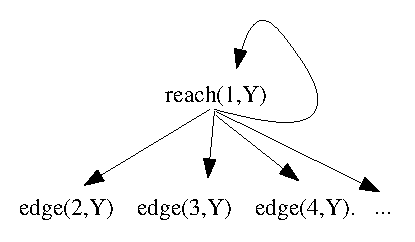
\includegraphics[width=\textwidth]{recursion}
%  \caption{Without \abstraction}
%  \label{fig:minipage1}
\end{minipage}
\quad
\begin{minipage}[b]{0.25\linewidth}
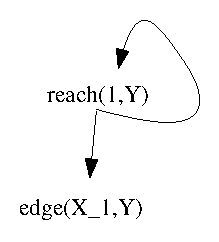
\includegraphics[width=0.5\textwidth]{abs-recursion}
%  \caption{With \abstraction}
%  \label{fig:minipage2}
\end{minipage}
\caption{A left-linear program and schematic IDGs: Left
  without IDG abstraction; Right: with
  IDG abstraction} \label{fig:abstraction}
\end{figure}
%------------------------------------------------------------
Abstracting the {\tt edge/2} predicate has subtle differences from
abstracting tabled subgoals.
%  The implementation of subgoal
%abstraction for tabled subgoals was described in~\cite{RigS13},
As mentioned, the {\tt edge/2} predicate of
Fig.~\ref{fig:abstraction} is not tabled.  Furthermore, the actual
{\tt edge/2} subgoal itself should not be abstracted to depth 0 since
losing the first argument instantiation would prevent the use of
indexing.  Rather, only the IDG's representation of the subgoal
should be abstracted.  Abstraction of dynamic code for
the IDG can be specified via the declaration:
\begin{center}
{\tt :-dynamic edge/2 as incremental, abstract(0)}.
\end{center}

In \version{} dynamic incremental code can be abstracted, but
incremental interned tries (Section~\ref{sec:incr-update-tries})
cannot be.  Also, currently only depth 0 abstraction is supported.

\subsection{Summary and Implementation Status}
%
When using incremental tabling an application will most commonly need
only the default transparent approach, although in special
circumstances eager updating may be desired.  The main design choices
are as usual what to table, and also what dynamic predicates or tries
should be made incremental.  In addition, performance optimizations
may be made through a mixture of subgoal abstraction and dynamic
predicate abstraction.  This optimization can be informed by use of
{\tt statistics/0} which includes summary information about the IDG,
or using the IDG inspection predicates of
Section~\ref{sec:incr-preds1} if more details is needed.

%Thus the user has four choices: tables may be
%updated as soon as the database is changed (e.g., via {\tt
%  incr\_assert/1}); at some point after a series of database changes
%(e.g. via {\tt incr\_assert\_inval/1} and {\tt
%  incr\_table\_update/0}); or lazily whenever a given table is called.
%In addition, if the changes are so massive that there is no point in
%incrementally updating the table, the tables can be abolished so that
%the tables will be reconstructed whenever they are re-queried.

In the current version of XSB, incremental tabling has not yet been
ported to the multi-threaded engine.  In addition, incremental tabling
only works for predicates that use both call and answer variance.
However, incremental tabling does work with for the full well-founded
semantics, for trie indexed dynamic code (in addition to regular
dynamic code) and with interned tries as described in
Section~\ref{sec:incr-update-tries}.  The space reclamation predicates
{\tt abolish\_all\_tables/0}, {\tt abolish\_table\_call/[1,2]} and
{\tt abolish\_table\_pred/[1,2]} can be safely used with incremental
tables.

\subsection{Predicates for Incremental Table Maintenance} \label{sec:incr-preds1}

\paragraph{A Note on Terminology}
%
Suppose {\tt p/1} and {\tt q/1} are incrementally tabled, and that
there is a clause
%
\begin{verbatim}
p(X):- q(X).
\end{verbatim}
%
In this case we say that {\tt p(X)} {\em depends\_on} {\tt q(X)} and
that {\tt q(X)} {\em affects} {\tt p(X)}.  A recursive predicate both
depends on and affects itself.


\paragraph{Declarations} The following directives support incremental
tabling based on changes in dynamic code: 

\index{tabling!opaque}
\index{tabling!declarations}
\begin{description}
\index{tabling!incremental}

\ourstandarditem{table +PredSpecs as incremental}{table/1}{Tabling}
%
is a executable predicate that indicates that each tabled predicate
specified in {\tt PredSpec} is to have its tables maintained
incrementally.  {\tt PredSpec} is a list of skeletons, i.e. open
terms, or {\tt Pred/Arity} specifications~\footnote{No explicit module
  references are allowed.}.  The tables must use call variance and
answer variance and must be compiled and loaded into the
single-threaded engine.  If a predicate is declared with tabling
attributes that are not supported with incremental tabling a
permission error is thrown.  This predicate implies that its arguments
are tabled predicates.  See page \pageref{table-declaration} for
further discussion of tabling options.

We also note that any tabled predicate that is called by a predicate
tabled as incremental must also be tabled as incremental or as opaque.
On the other hand, a dynamic predicate {\tt d/n} that is called by a
predicate tabled as incremental may or may not need to be declared as
incremental.  However if {\tt d/n} is not declared incremental, then
changes to it will not be propagated to incrementally maintained
tables.

\ourstandarditem{dynamic +PredSpecs as incremental}{dynamic/1}{Tabling}
%
is an executable predicate that indicates that each predicate in {\tt
  PredSpecs} is dynamic and used to define an incrementally tabled
predicate and will be updated using {\tt incr\_assert/1} and/or {\tt
  incr\_retractall/1} (or relatives.)  Note that dynamic incremental
predicates cannot themselves be tabled.  This predicate implies that
its arguments are dynamic predicates.  See page
\pageref{dynamic-declaration} for further discussion of dynamic
options.

\ourstandarditem{table +PredSpecs as opaque}{table/1}{Tabling} 
%
is an executable predicate that indicates that each predicate $P$ in
{\tt PredSpecs} is tabled and is used in the definition of some
incrementally tabled predicate but should not be maintained
incrementally.  In this case the system assumes that the programmer
will abolish tables for $P$ in such a way so that re-calling it will
always give semantically correct answers.  In other words, instead of
maintaining information to support incremental table maintenance, the
system re-calls the opaque predicate whenever its results are required
to recompute an answer.  One example of an appropriate use of opaque
is for tabled predicates in a DCG used to parse some string.  Rather
than incrementally maintain all dependencies on all input strings, the
user can declare these intermediate tables as opaque and abolish them
before any call to the DCG.  This predicate implies that its arguments
are tabled predicates.

\end{description}

\paragraph{Basic Incremental Maintenance Predicates}
The following predicates are used to manipulate incrementally
maintained tables:

\begin{description}
\ourrepeatmoditem{incr\_assert(+Clause)}{incr\_assert/1}{increval} 
\ourrepeatmoditem{incr\_assertz(+Clause)}{incr\_assertz/1}{increval}
\ourrepeatmoditem{incr\_asserta(+Clause)}{incr\_asserta/1}{increval}
\ourrepeatmoditem{incr\_retract(+Clause)}{incr\_retract/1}{increval}
\ourmoditem{incr\_retractall(+Term)}{incr\_retractall/1}{increval}
% 
are versions of {\tt assert/1} and other standard Prolog predicates.
They modify dymamic code just as their Prolog counterparts, but they
then invalidate all incrementally maintained tables that depend on
{\tt Clause}.

{\bf Error Cases} are the same as {\tt assert<a/z>/1}, {\tt retract/1}
and {\tt retractall/1} with the additional error condition:

\begin{itemize}
\item The head of the clause {\tt Clause} or the {\tt Term} refers to
  a predicate that is not incremental and dynamic.  
\bi
\item  {\tt type error(dynamic\_incremental, Term)}
\ei
\end{itemize}

\ourrepeatmoditem{incr\_assert\_update(+Clause)}{incr\_assert\_update/1}{increval}
\ourrepeatmoditem{incr\_assertz\_update(+Clause)}{incr\_assertz\_update/1}{increval}
\ourrepeatmoditem{incr\_asserta\_update(+Clause)}{incr\_asserta\_update/1}{increval}\
\ourrepeatmoditem{incr\_retractall\_update(+Clause)}{incr\_retractall\_update/1}{increval}
\ourmoditem{incr\_retract\_update(+Term)}{incr\_retract\_update/1}{increval}
%
are versions of {\tt assert/1} and other standard Prolog predicates.
They modify dymamic code just as their Prolog counterparts, mark any
incrementally maintained tables that depend on the modification as
invalid, then immediately update these tables.
%  The tables may be updated by an
%explicit call to {\tt incr\_table\_update/[0,1,2]}, or the table will
%be dynamically recomputed when a query is made to it.

\ourmoditem{incr\_table\_update}{incr\_table\_update/0}{increval} may
be called after base predicates have been changed (by {\tt
  incr\_assert/1} and/or {\tt incr\_retract/1} or friends).  This
predicate updates all the incrementally maintained tables whose
contents may be affected by those changes to the base predicates.
%This update operation is separated from the operations that change the
%base predicates ({\tt incr\_assert\_inval/1} and {\tt
%  incr\_retractall\_inval/1}) so that a set of base predicate changes
%can be processed all at once, which may be much more efficient that
%updating the tables at every base update.  Beginning with Version
%3.3.7, it is not absolutely necessary to call this predicate, as
%tables will be incrementally updated upon demand.  However, using this
%predicate allows a choice of incurring the cost of update at a time
%other than querying an updated goal.
Explicit update calls only need to be used in special circumstances
(cf. Section~\ref{sec:incr-eager}).

{\bf Error Cases}
\bi
\item A table $T$ that is to be incrementally updated is not yet
  complete.  
\bi
\item 	{\tt permission\_error(update, incomplete\_table Goal)}
\ei
\ei

\ourmoditem{incr\_table\_update(-GoalList)}{incr\_table\_update/1}{increval}
acts as {\tt incr\_table\_update/0} in its action to update the
incrementally maintained tables after changes to base predicates.  It
returns the list of goals whose tables were changed in the update
process.

\ourmoditem{incr\_table\_update(+SkelList,-GoalList)}{incr\_table\_update/2}{increval}
acts as {\tt incr\_table\_update/1} in its action to update
incrementally maintained tables after changes to base predicates.  The
first argument is a list of predicate skeletons (open terms) for
incrementally maintained tables.  The predicate returns in {\tt
  GoalList} a list of goals whose skeletons appear in {\tt SkelList}
and whose tables were changed in the update process.  In this way {\tt
  SkelList} acts as a filter to restrict the goals that are returned
to those of interest.  If {\tt SkelList} is a variable, all affected
goals are returned in {\tt GoalList}.

\ourmoditem{incr\_invalidate\_call(+Goal)}{incr\_invalidate\_call/1}{increval}
is used to directly invalidate a call to an incrementally maintained
table, {\tt Goal}.  A subsequent call to {\tt Goal} will automatically
perform incremental updating for {\tt Goal} along with any tables that
{\tt Goal} depends on that are in need of updating; similarly an
invocation of {\tt incr\_table\_update/[0,1,2]} will cause {\tt Goal}
to be recomputed along with all incrementally maintained tables that
{\tt Goal} affects.  This predicate can be used if a tabled predicate
depends on some external data and not (only) on dynamic incremental
predicates.  For example, if an incrementally maintained predicate
depends on a relation stored in an external relational database
(perhaps accessed through the ODBC interface), then this predicate can
be used to invalidate the table when the external relation changes.
The application programmer must know when the external relation
changes and invoke this predicate as necessary.

{\bf Error Cases}
\bi
\item 	{\tt Goal} is tabled, but not incrementally tabled
\bi
\item 	{\tt permission\_error(invalidate,non-incremental predicate,Goal)}
\ei
\ei

\end{description}

\paragraph{Incremental Maintenance using Interned Tries}
The following predicates are used to modify incremental tries, and can
be freely intermixed with predicates for modifying incremental dynamic
code, as well as with predicates for invalidating or updating tables
(Section~\ref{sec:incr-preds1}).

\begin{description}
\ourmoditem{incr\_trie\_intern(+TrieIdOrAlias,+Term)}{incr\_trie\_intern/2}{intern}
%
is a version of {\tt trie\_intern/2} for tries declared as
incremental.  A call to this predicate interns {\tt Term} in {\tt
  TrieIdOrAlias} and then invalidates all incrementally maintained
tables that depend on this trie.

\ourmoditem{incr\_trie\_uninternall(+TrieIdOrAlias,+Term)}{incr\_trie\_uninternall/2}{intern}
%
is a version of {\tt trie\_unintern/2} for tries declared as
incremental.  A call to this predicate removes all terms unifying with
{\tt Term} in {\tt TrieIdOrAlias} and then invalidates all
incrementally maintained tables that depend on this trie.

\ourmoditem{incr\_trie\_intern\_update(+TrieIdOrAlias,+Term)}
           {incr\_trie\_intern\_update/2}{intern}
%
works for tries declared as incremental in a similar manner as {\tt
  incr\_trie\_intern/2} except that it also immediatesly updates any
affected tables.

\ourmoditem{incr\_trie\_uninternall\_inval(+TrieIdOrAlias,+Term)}
{incr\_trie\_uninternall\_inval/2}{intern}
%
works for tries declared as incremental in a similar manner as {\tt
  incr\_trie\_uninternall/2} except that it also immediately updates
any affected tables.
\end{description}

\index{residual dependency graph}
\index{incremental dependency graph}
\paragraph{Inspecting Dependencies among Incremental Subgoals}
%
% These relations form a labelled directed graph for which the
%nodes are incrementally tabled subgoals present in XSB; a given
%subgoal in the graph may or may not have been completed.  
%Conceptually, there is an edge from $S_1$ to $S_2$ labelled depends
%(affects) if $S_1$ directly depends on (directly affects) $S_2$.  We
%call this graph the {\em incrementally tabled subgoal dependency
%  graph}, or just the incremental dependency graph.  
The predicates in this section allow a user to inspect properties of
IDG that can be useful in debugging, profiling or optimizing a
computation~\footnote{The predicates for traversing the incremental
  dependency graph are somewhat analogous to those for traversing the
  residual dependency graph (Section~\ref{sec:table-inspection}).}.

As explained below, IDG nodes can be accessed via the predicate {\tt
  is\_incremental\_subgoal/1}, while IDG edges can be accessed via
{\tt incr\_directly\_depends/2}.  The predicates {\tt
  get\_incr\_scc/[1,2]} and {\tt get\_incr\_scc\_with\_deps/[3,4]} can
be used to efficiently materialize the dependency graph in Prolog,
including SCC information.

\begin{description}

\ourmoditem{is\_incremental\_subgoal(?Subgoal)}{is\_incremental\_subgoal/1}{increval}
%
This predicate non-deterministically unifies {\tt Subgoal} with
incrementally tabled subgoals that are currently table entries.

\ourmoditem{incr\_directly\_depends(?Goal$_1$,?Goal$_2$)}{incr\_directly\_depends/2}{increval}
accesses the edges of the IDG: the incremental goals (Tables) that
directly depend on or directly affect one another.  At least one of
{\tt Goal$_1$} or {\tt Goal$_2$} must be bound.
\begin{itemize}
\item If {\tt Goal$_1$} is bound, then this predicate will return in
  {\tt Goal$_2$} through backtracking the goals for all incrementally
  maintained tables on which {\tt Goal$_1$} directly depends.
\item If {\tt Goal$_2$} is bound, then it returns in {\tt Goal$_1$}
  through backtracking the goals for all incrementally maintained
  tables that {\tt Goal$_2$} directly affects -- in other words all
  goals that directly depend on {\tt Goal$_2$}.  \ei

{\bf Error Cases}
\bi
\item Neither {\tt Goal$_1$} nor {\tt Goal$_2$} is bound 
\bi
\item 	{\tt instatiation\_error}
\ei
\item {\tt Goal$_1$} and/or {\tt Goal$_2$} is bound, but is not
  incrementally tabled
\bi
\item 	{\tt table\_error}
\ei
\ei

\ourmoditem{incr\_trans\_depends(?Goal$_1$,?Goal$_2$)}{incr\_trans\_depends/2}{increval}
is similar to {\tt incr\_directly\_depends/2} except that it returns
goals according to the transitive closure of the ``directly depends''
relation.  Error conditions are the same as {\tt
  incr\_directly\_depends/2}.

\ourrepeatmoditem{get\_incr\_sccs(?SCCList)}{get\_incr\_sccs/1}{increval}
\ourrepeatmoditem{get\_incr\_sccs\_with\_deps(?SCCList,?DepList)}{get\_incr\_sccs\_with\_deps/2}{increval}
\ourrepeatmoditem{get\_incr\_sccs(+SubgoalList,?SCCList)}{get\_incr\_sccs/2}{increval}
\ourmoditem{get\_incr\_sccs\_with\_deps(+SubgoalList,?SCCList,?DepList)}{get\_incr\_sccs\_with\_deps/3}{increval}
%
Most linear algorithms for SCC detection over a graph use destructive
assignment on a stack to maintain information about the connecteness
of a component; as a result such algorithms are
difficult to write efficiently in Prolog.

{\tt get\_incr\_sccs/1} unifies {\tt SCCList} with SCC information for
the incremental dependency graph that is represented as a list whose
elements are of the form
\begin{center}
{\tt ret(Subgoal,SCC)}.
\end{center}
{\tt SCC} is a numerical index for the SCCs of Subgoal. Two subgoals
are in the same SCC iff they have the same index, however no other
dependency information can be otherwise directly inferred from the
index~\footnote{The actual number for each SCC index depends on how
  the incremental dependency graph happens to be traversed; as a
  result it is best to rely on the index only as a ``generated'' name
  for each SCC.}.

If dependency information is also desired, {\tt
  get\_incr\_scc\_with\_dependencies/2} should be called.  In addition
to the SCC information as above, {\tt DepList} is unified with a list
of dependency terms of the form
\begin{center}
{\tt depends(SCC1,SCC2)}
\end{center}
for each pair {\tt SCC1} and {\tt SCC1} such that some subgoal with
index {\tt SCC1} directly depends on some subgoal with index {\tt
  SCC1}.  If it is necessary to know which subgoal(s) in {\tt SCC1}
directly depends on which subgoal(s) in {\tt SCC2}, the information
can be easily reconstructed using {\tt incr\_directly\_depends/2}
above.  Similarly, {\tt incr\_directly\_depends/2} can be used to
determine the actual edges within a given SCC.

Ordinarily a user will want to see the entire dependency graph and in
such a case the predicates described above should be used.  However,
note that if the dependency graph is the result of several
indepdendent queries it may not be connected.  {\tt get\_incr\_scc/2}
takes as input a list of incremental subgoals, {\tt SubgoalList}.  For
each {\tt Subgoal} in {\tt SubgoalList}, this predicate finds the set
of subgoals connected to {\tt Subgoal} by any mixture of depends and
affects relations, unions these sets together, and finds the SCCs of
all subgoals in the unioned set.

SCC detection is implemented using Tarjan's algorithm~\cite{Tarj72} in
C working directly on XSB's data structures.  The algorithm is
$\cO(|V| + |E|)$ where $|V|$ is the number of vertices and $|E|$ the
number of edges in the dependency graph.  As a result, {\tt
  get\_incr\_sccs/[1,2]} provides an efficient means to materialize the
  high-level topography of the dependency graph~\footnote{Currently,
    the materialization of dependency information between SCCs is
    implemented in a naive manner, so that {\tt
      get\_incr\_sccs\_with\_deps/[2,3]} is $\cO(|V|^2)$.}.

{\bf Error Cases}
\bi
\item {\tt SCCList} contains a predicate that is not tabled
\bi
\item 	{\tt permission\_error}
\ei
\ei
\end{description}

 (included in tables)
\chapter{Standard Predicates and Predicates of General Use} \label{standard}
%=============================================

This chapter describes standard predicates, which are always available
to the Prolog interpreter, and do not need to be imported or loaded
explicitly as do other Prolog predicates.  By default, it is a
compiler error to redefine standard predicates.  

\comment{This behavior can be overridden by allowing explicit
  redefinition of standard predicates (see Section~\ref{}); or
  alternatively the set of standard predicates can be easily
  reconfigured (Section~\ref{}).}

In the description below, certain standard predicates depend on HiLog
semantics; the description of such predicates have the token {\sf
HiLog} at the right of the page.  Similarly predicates that depend on
SLG evaluation are marked as {\sf Tabling}, and predicates whose
semantics is defined by the ISO standard (or whose implementation is
reasonably close to that definition) are marked as {\tt ISO}.
Occasionally, however, we include in this section predicates that are
not standard.  In such cases we denote their module in {\tt text} font
towards the middle of the page.

\comment{
\paragraph*{A Note on Types} \label{sec:types}

Numerous proposals have been made concerning typing systems for Prolog
for the purposes of program analysis, correctness checking, etc.
Analysis-based typing systems are typically lattice-based, following
from their need to compare types to understand whether one type
includes another, or from the need to determine the most specific type
that is more general than two types.  In addition the ISO standard
specifies various types of allowable input or output arguments for
various predicates.

\version{} of XSB has the following approach to program typing.
Typing in an XSB program is done through a {\em type lattice},
generated by {\em primitive type elements}.  How a primitive type is
defined is somewhat separate from how it is used by a type lattice.
For our purposes we assume that each 1-ary type element is defined by
a predicate of arity 1 that is written in a pure enough style so that
its success or failure does not depend on the state of XSB or of any
external state.  Whether these types are recursive or not has no
bearing on the type lattice.  For instance, {\tt integer} or {\tt
listOfAtoms} are primitive type elements.  Similarly, {\tt variable},
{\tt ground} are also type elements.  We say that a given term {\tt
Term} satisfies a primitive type element {\tt t} if {\tt t(Term)}
succeeds.  Given primitive type elements, complex type elements can be
formed using the boolean operations, {\tt and}, {\tt or} and {\tt
not}.  As an example, {\tt integer or not(listOfAtoms)} is a
non-primitive type element.  There is also a product operation ({\tt
,}) on type elements, so that {\tt variable, integer or
not(listOfAtoms)} is a product of the above two types.  
Satisfiability is extended to complex type elements in the obvious
manner, and an n-ary typle of terms satisfies a n-ary product type if
each argument in the tuple satisfies the corresponding argument of the
product type.

The above description is not yet suitable for a type system as it
could not determine, for instance, that {\tt integer} is a subtype of
{\tt number}.  To determine this, an explicit {\em inclusion
statement} can be made indicating that one type is included in
another.  Thus given two elements in a type lattice with inclusion
statements, determining whether one element is more specific than
another can be done using techniques for propositional satisfiability
or stable model generation.

From an implementational level, types can be defined using the Cold
Dead Fish (CDF) package and inclusion can be detected using the CDF
theorem prover or XSB's Smodels interface.  However, for the
purposes in this section we use type elements to define inputs and
outputs of predicates, via {\tt usage statements}.  A usage statement
for an n-ary predicate {\tt p/n} consists of an n-ary product of
primitive types that should be satisfied on a call to {\tt p/n} along
with a n-ary product of primitive types that should hold on success of
{\tt p/n} given the types that hold at call.  If both the the product
types hold, the usage statement is satisfied.  Each successful call to
{\tt p/n} should satisfy one of the usage statements.

As defined, usage statements are very general: they can check not only
traditional Prolog types ({\tt atom}, {\tt integer}, etc), but also
non-Prolog types, such as the fact that the input to a given argument
should be a positive integer, and even instantiation patterns.  For
the various predicates defined in this section, we use the following
conventions for usages and error reporting.  {\bf domain}, {\bf type}
and {\bf instantiation} errors arise from the failure of an argument
of a predicate to satisfy the corresponding type element in the input
term of the usage statements.  All of these could be called type
errors given the system described above.  However to (partially)
conform to the ISO standard, we reserve the {\bf instantiation error}
to mean failure that occurs when an argument does not satisfy a type
in a boolean lattice generated by {\tt var} and {\tt ground}.  A {\bf
  type error} occurs when an argument does not satisfy a type in a
boolean lattice generated by other ISO types, such as {\tt integer},
{\tt atom}, etc.  A {\bf domain error} arises from other such errors.
We note that in certain cases, our designation of an error type may
differ from the ISO standard.
}

%--------------------------------------------------------------------------------------------------
\section{Input and Output}
\index{streams}

XSB's I/O is based on ISO-style streams, although it also supports
older DEC-10 style file handling.  The use of streams provides a
unified interface to a number of different classes of sources and
sinks.  Currently these classes include textual and binary files,
console input and output, pipes, and atoms; in the future sockets and
urls may be handled under the stream interface.  When streams are
opened, certain actions may occur depending on the class of the source
or sink and on the wishes of the user.  For instance when a file {\tt
F} is opened for output mode, an existing file {\tt F} may be
truncated (in write mode) or not (in append mode).  In addition,
various operations may or may not be valid depending on the class of
stream.  For instance, repositioning is valid for an atom or file but
not a pipe or console.

XSB provides several default I/O streams, which make it easier for a
user to embed XSB in other applications.  These streams include the
default input and output streams.  They also include the standard
error stream, to which XSB writes all error messages.  By default the
standard error stream is the same as the standard output stream, but
it can be redirected either by UNIX shell-style I/O redirection or by
the predicates {\tt file\_reopen/4} and {\tt file\_clone/3}.
Similarly there is the standard warning stream (to which all system
warnings are written), the standard message stream, the standard
debugging stream (to which debugging information is written), and the
standard feedback stream (for interpreter prompts, yes/no answers,
etc).  All of these streams are aliased by default to standard output,
and can be redirected by the predicates the predicates {\tt
  file\_reopen/4} and {\tt file\_clone/3}.

\index{aliases!streams}
Streams may also be aliased: the default input and output streams can
be denoted by {\tt user\_input} and {\tt user\_output} and they refer
to the standard input and standard output streams of the
process \footnote{For backwards compatibility, the default input
  stream can also be aliased by {\tt user} or {\tt userin}, and the
  default output stream by {\tt user} or {\tt userout}.}.  Similarly,
XSB's error, warning and message streams user the aliases {\tt
  user\_error}, {\tt user\_warning} and {\tt user\_message}
respectively (cf. Section~\ref{}).

Streams are distinguished by their {\tt class} -- whether they are
file or atom, etc.; as well as by various properties.  These
properties include whether a stream is positionable or not and whether
a (file) stream is textual or binary.

\bi
\item {\tt Console} The default streams mentioned above are
console streams, which are textual and not repositionable.
%
\item {\tt File}  A file stream corresponds to an operating system
file and is repositionable.  On Windows, binary files and textual
files differ, while on UNIX they are the same.  
%
\item {\tt Atom} XSB can read from an atom, just as it can from a file.
Atoms are considered to be textual and repositionable.  Writing to
atoms via streams is not currently available in XSB, although 
the predicate {\tt term\_to\_atom/[2,3]} contains much of the
functionality that such streams would provide.

\item {\tt Pipe} XSB can also open pipes either directly, or as part
of its ability to spawn processes.  When made into streams, pipes are
textual and not repositionable.
\ei

%------------------------------------------------------------------------------------------------
\subsection{I/O Stream Implementation} \label{sec:IO-streams}

A user may note that XSB's I/O streams are small integers, but they
should not be confused with the file descriptors used by the OS.  The
OS file descriptors are objects returned by the C {\tt open} function;
XSB I/O streams indices into the internal XSB table of open files and
associated information. The OS does not know about XSB I/O streams,
while XSB (obviously) does know about the OS file descriptors. An OS
file descriptor may be returned by certain predicates (e.g.  {\tt
pipe\_open/2} or user-defined I/O).  In the former case, a file
descriptor can be promoted to XSB stream by {\tt open/\{3,4\}} and in
the latter by using the predicate {\tt fd2iostream/2}.

When it starts, XSB opens a number of standard I/O streams that it
uses to print results, errors, debugging info, etc. The descriptors
are described in the file {\tt prolog\_includes/standard.h}. This file
provides the following symbolic definitions:
%%
\begin{verbatim}
    #define STDIN            0
    #define STDOUT           1
    #define STDERR           2
    #define STDWARN          3    /* output stream for xsb warnings  */
    #define STDMSG           4    /* output for regular xsb messages */
    #define STDDBG           5    /* output for debugging info       */
    #define STDFDBK          6    /* output for XSB feedback
                                     (prompt/yes/no/Aborting/answers) */

    #define AF_INET     0     /* XSB-side socket request for Internet domain */
    #define AF_UNIX     1     /* XSB-side socket request for UNIX domain */
\end{verbatim}
%%
%------------------------------------------------------------------------------------------
\comment{
In addition, the file \verb|emu/file_modes_xsb.h| provides the definitions
for the file opening modes:
%%
\begin{verbatim}
    #define OREAD          0    /* open for read           */
    #define OWRITE         1    /* open for write          */
    #define OAPPEND        2    /* open for append         */
    #define OSTRINGR       3    /* open string for reading */
    #define OSTRINGW       4    /* open string for writing (not implemented) */
\end{verbatim}
%%
}
%------------------------------------------------------------------------------------------
These definitions can be used in user programs, if the following is
provided at the top of the source file:
%%
\begin{verbatim}
    compiler_options([xpp_on]).
    #include "standard.h"
\end{verbatim}
%%
If this header is used, the various streams can be used as any other output stream -- e.g. 
{\tt ?- write(STDWARN,'watch it!')}.
%
(Note: the XSB preprocessor is not invoked on clauses typed into an
interactive XSB session, so the above applies only to programs loaded from
a file using {\tt consult} and such.)

\subsection{ISO Streams}

\begin{description}

\isoitem{open(+SourceSink,+Mode,-Stream)}{open/3}
%
{\tt open/1} creates a stream for the source or sink designated in
{\tt SourceSink}, and binds {\tt Stream} to a structure representing
that stream.  
%
\bi
\item If {\tt SourceSink} is an atom, or the term {\tt file(File)}
where {\tt File} is an atom, the stream is a file stream.  In this
case {\tt Mode} can be 
\bi
\item {\tt read} to create an input stream.  In Windows, whether the
file is textual or binary is determined by the file's properties.
%
\item {\tt write} to create an output stream.  Any previous file with
a similar path is removed and a (textual) file is created which becomes
a record of the output stream.  
%
\item {\tt write\_binary} to create an output stream.  Any previous file with
a similar path is removed and a file is created which becomes
a record of the output stream.  The file created is binary in Windows,
while in UNIX {\tt write\_binary} has the same effect as {\tt write}.
%
\item {\tt append} to create an output stream.  In this case the
output stream is appended to the contents of the file, if it exists,
and otherwise a new file is created for (textual) output
%
\item {\tt append\_binary} to create an output stream.  In this case the
output stream is appended to the contents of the file, if it exists,
and otherwise a new file is created for (binary) output
\ei
\item If {\tt SourceSink} is the term {\tt atom(Atom)} where {\tt
Atom} is an atom, the stream is an atom stream.  In this case {\tt
Mode} currently can only be {\tt read}.  This stream class, which
reads from interned atoms, is analogous to C's {\tt sscanf()}
function.
%
\item If {\tt SourceSink} is the term {\tt pipe(FIleDescriptor)}
where {\tt FileDescriptor} is an integer, then a pipe stream is opened
in the mode for {\tt FileDescriptor}.
\ei

\compatability This predicate extends the ISO definition of {\tt
open/3} to include strings and pipes as well as the file modes {\tt
write\_binary} and {\tt append\_binary}.

{\bf Error Cases}
\bi
\item 	{\tt SourceSink} or {\tt Mode} is not instantiated
\bi
\item 	{\tt instantiation\_error}
\ei
%
\item 	{\tt Mode} is not a valid I/O mode
\bi
\item 	{\tt domain\_error(io\_mode,Mode)}
\ei
%
\item 	{\tt SourceSink} is a file and cannot be opened, or opened in
the desired mode 
\bi
\item 	{\tt permission\_error(open,file,SourceSink)}
\ei
\ei

\isoitem{open(+File,+Mode,-Stream,+Options)}{open/4}
%
{\tt open/4} behaves as does {\tt open/3}, but allows a list of
options to be given.  The current options are a subset of ISO options
and are:
\bi
\item {\tt alias(A)} allows the stream to be aliased to an atom {\tt
  A}.
%
\item {\tt type(T)} has no effect on file streams in UNIX, which are
  always textual, but in Windows if {\tt T} is {\tt binary} a binary
  file is opened.
\ei
%
{\bf Error Cases}  Error cases are the same as {\tt open/3} but with
the addition: 
\bi
\item {\tt Option\_list} contains an option {\tt O} that is not a
  (currently implemented) stream option.  
\bi
\item {\tt domain\_error(stream\_option,O)}
\ei
\item An element of {\tt OptionsList} is alias(A) and A is already
  associated with an existing thread, queue, mutex or stream 
\bi
\item {\tt permission\_error(create,alias, A)}
\ei
\item An element of {\tt OptionsList} is alias(A) and A is not an atom
\bi
\item {\tt type\_error(atom,A)}
\ei
\ei
%
\compatability 
%
The ISO option {\tt reposition(Boolean)} currently has no effect on
streams, because whether or not the stream is repositionable or not
depends on the stream class.  The ISO option {\tt eof\_action(Action)}
currently has no effect on file streams.  If these options are
encountered in {\tt Options}, a warning is issued to {\tt STDWARN}.

\isoitem{close(+Stream\_or\_alias,+OptionsList)}{close/2}
%
{\tt close/2} closes the stream or alias {\tt Stream\_or\_alias}.
{\tt OptionsList} allows the user to declare whether a permission
error will be raised in XSB upon a resource or system error from the
closing function (e.g. {\tt fclose()} or other system function).  If
{\tt OptionsList} is non-empty and contains only terms unifying with
{\tt force(true)} then such an error will be ignored (possibly leading
to unacknowledged loss of data).  Otherwise, a permission error is
thrown if {\tt fclose()} or other system function returns an error
condition.  If the stream class of {\tt Stream\_or\_alias} is an atom,
then the only action taken is to close the stream itself -- the
interned atom itself is not affected.

{\bf Error Cases}
\bi
\item 	{\tt Stream\_or\_alias} is a variable
\bi
\item {\tt instantiation\_error}
\ei
\item {\tt Stream\_or\_alias} is neither a variable, nor a stream term
  nor an alias.  
\bi
\item 	{\tt domain\_error(stream\_or\_alias,Stream\_or\_alias)}
\ei
\item 	{\tt Stream\_or\_alias} is not associated with an open stream
\bi
\item 	{\tt existence\_error(stream,Stream\_or\_alias)}
\ei
\item {\tt OptionList} contains an option {\tt O} that is not a closing
option.
\bi
\item {\tt domain\_error(close\_option,O)}
\ei
\item {\tt OptionList} contains conflicting options
\bi
\item {\tt domain\_error(close\_option,OptionList)}
\ei
\item 	Closing the stream produces an error (and {\tt OptionsList} is
	a non-empty list containing terms of the form {\tt force(true)}).
\bi
\item 	{\tt permission\_error(close,file,Stream\_or\_alias)}
\ei
\ei

\isoitem{close(+Stream\_or\_alias)}{close/1}
%
{\tt close/1} closes the stream or alias {\tt Stream\_or\_alias}.\\
Behaves as {\tt close(Stream\_or\_alias,[force(false)])}.

\isoitem{set\_input(+Stream\_or\_alias)}{set\_input/1}
    Makes file {\tt Stream\_or\_alias} the current input stream. 

{\bf Error Cases}
\bi
\item 	{\tt Stream\_or\_alias} is a variable
\bi
\item {\tt instantiation\_error}
\ei
\item {\tt Stream\_or\_alias} is neither a variable, nor a a stream
  term nor an alias.  
\bi
\item 	{\tt domain\_error(stream\_or\_alias,Stream\_or\_alias)}
\ei
\item 	{\tt Stream\_or\_alias} is not an open input stream
\bi
\item 	{\tt existence\_error(stream,Stream\_or\_alias)}
\ei
\ei

\isoitem{set\_output(+Stream\_or\_alias)}{set\_output/1}
    Makes file {\tt Stream\_or\_alias} the current output stream. 

{\bf Error Cases}
\bi
\item 	{\tt Stream\_or\_alias} is a variable
\bi
\item {\tt instantiation\_error}
\ei
\item {\tt Stream\_or\_alias} is neither a variable, nor a a stream
  term nor an alias.  
\bi
\item 	{\tt domain\_error(stream\_or\_alias,Stream\_or\_alias)}
\ei
\item 	{\tt Stream\_or\_alias} is not associated with an open output stream
\bi
\item 	{\tt existence\_error(stream,Stream\_or\_alias)}
\ei
\ei

\isoitem{stream\_property(?Stream,?Property)}{stream\_property/2}
%
This predicate backtracks through the various stream properties that
unify with {\tt Property} for the stream {\tt Stream}.  Currently,
the following properties are defined.

\bi
\item {\tt stream\_class(C)} gives the stream class for a file:
i.e. {\tt file}, {\tt atom}, {\tt console} or {\tt pipe}.

\item {\tt file\_name(F)} is a property of {\tt Stream}, if
{\tt Stream} is a file stream and {\tt F} is the file name
associate with {\tt Stream}.  The full operating system
path is used.
%
\item {\tt type(T)} is a property of {\tt Stream}, if
{\tt Stream} is a file stream and {\tt T} is the file type
of {\tt Stream}: {\tt text} or {\tt binary}.
%
\item {\tt mode(M)} is a property of {\tt Stream}, if {\tt
M} represents the I/O mode with which {\tt Stream} was
opened: i.e. {\tt read}, {\tt write}, {\tt append}, {\tt
write\_binary}, etc., as appropriate for the class of {\tt
Stream}.
%
\item {\tt alias(A)}  is a property of {\tt Stream}, if
{\tt Stream} was opened with alias {\tt A}.
%
\item {\tt input}  is a property of {\tt Stream}, if {\tt
Stream} was opened in the I/O mode: {\tt read}.
% 
\item {\tt output}  is a property of {\tt Stream}, if {\tt
Stream} was opened in the I/O mode: {\tt write}, {\tt
append}, {\tt write\_binary}, or {\tt append\_binary}.
%
\item {\tt reposition(Bool)} is true, if {\tt Stream} is
repositionable, and false otherwise. 
%
\item {\tt end\_of\_stream(E)} returns {\tt at} if the end of stream
condition for {\tt Stream} is true, and {\tt not} otherwise.
%
\item {\tt position(Pos)} returns the current position of the stream
as determined by {\tt fseek{}} or the byte-offset of the current
stream within an atom.  In either case, if an end-of-stream condition
occurs, the token {\tt end\_of\_file} is returned.
%

%
\item {\tt eof\_action(Action)} is {\tt reposition} if the stream class
is {\tt console}, {\tt eof\_code} if the stream class is {\tt file},
and {\tt error} is the stream class is {\tt pipe} or {\tt atom}.
\end{itemize}

\isoitem{flush\_output(+Stream\_or\_alias)}{flush\_output/1}
%
Any buffered data in {\tt Stream\_or\_alias}  gets flushed.  If
{\tt Stream} is not buffered (i.e. if it is of class {\tt
atom}), no action is taken.

{\bf Error Cases}
\bi
\item 	{\tt Stream\_or\_alias} is a variable
\bi
\item {\tt instantiation\_error}
\ei
\item {\tt Stream\_or\_alias} is neither a variable, nor a a stream
  term nor an alias.  
\bi
\item 	{\tt domain\_error(Stream\_or\_alias,Stream)}
\ei
\item 	{\tt Stream} is not associated with an open output stream 
\bi
\item 	{\tt existence\_error(Stream\_or\_alias,Stream)}
\ei
\item 	Flushing (i.e. {\tt fflush()}) returns an error.
\bi
\item 	{\tt permission\_error(flush,stream,Stream)}
\ei
\ei

\isoitem{flush\_output}{flush\_output/0}
%
Any buffered data in the current output stream gets flushed.

\isoitem{set\_stream\_position(+Stream\_or\_alias,+Position)}{set\_stream\_position/2}
%
If the stream associated with {\tt Stream\_or\_alias} is
repositionable (i.e. is a file or atom), sets the stream position
indicator for the next input or output operation. Position is a
positive integer, taken to be the number of bytes the stream is to be
placed from the origin.

{\bf Error Cases}
\bi
\item 	{\tt Stream\_or\_alias} is a variable
\bi
\item {\tt instantiation\_error}
\ei
\item {\tt Stream\_or\_alias} is neither a variable, nor a a stream
  term nor an alias.  
\bi
\item 	{\tt domain\_error(stream\_or\_alias,Stream\_or\_alias)}
\ei
\item 	{\tt Position} is not instantiated to a positive integer.
\bi
\item 	{\tt domain\_error(stream\_position,Position)}
\ei
\item 	{\tt Stream\_or\_alias} is not associated with an open stream
\bi
\item 	{\tt existence\_error(stream,Stream\_or\_alias)}
\ei
\item 	{\tt Stream\_or\_alias} is not repositionable, or
	repositioning returns an error. 
\bi
\item 	{\tt permission\_error(resposition,stream,Stream\_or\_alias)}
\ei
\ei

\isoitem{at\_end\_of\_stream(+Stream\_or\_alias)}{at\_end\_of\_stream/1}
%
Succeeds if {\tt Stream\_or\_alias} has position at or past the end of
stream.

{\bf Error Cases}
\bi
\item 	{\tt Stream\_or\_alias} is a variable
\bi
\item {\tt instantiation\_error}
\ei
\item {\tt Stream\_or\_alias} is neither a variable, nor a a stream
  term nor an alias.  
\bi
\item 	{\tt domain\_error(stream,Stream\_or\_alias)}
\ei
\item 	{\tt Stream\_or\_alias} is not an open stream
\bi
\item 	{\tt existence\_error(stream,Stream\_or\_alias)}
\ei
\ei
%

\isoitem{at\_end\_of\_stream}{at\_end\_of\_stream/0}
%
Acts as {\tt at\_end\_of\_stream/1} but using the current input
stream.

\end{description}

\subsubsection{Other Predicates using ISO Streams}

\begin{description}

\standarditem{file\_reopen(+FileName,+Mode,+Stream,-RetCode)}{file\_reopen/3}
%
    Takes an existing I/O stream, closes it, then opens it and
    attaches it to a file. This can be used to redirect I/O from any of the
    standard streams to a file. For instance, 
%%
\begin{verbatim}
    | ?- file_reopen('/dev/null', w, 3, Error).
\end{verbatim}
%%
    redirects all warnings to the Unix black hole. 

    On success, {\tt RetCode} is 0; on error, the return code is negative.

%-----------------------------------------------------------------------------

\standarditem{file\_clone(+SrcStream,?DestStream,-RetCode)}{file\_clone/3}
%
This is yet another way to redirect I/O. It is a Prolog interface to
the C {\tt dup} and {\tt dup2} system calls. If {\tt DestStream} is a
variable, then this call creates a new XSB I/O stream that is a clone
of {\tt SrcStream}. This means that I/O sent to either stream goes
to the same place. If {\tt DestStream} is not a variable, then it must
be a number corresponding to a valid I/O stream. In this case, XSB
closes {\tt DestStream} and makes it into a clone of {\tt
SrcStream}. 

For instance, suppose that 10 is a I/O Stream that is currently open
for writing to file {\tt foo.bar}.  Then 
%%
\begin{verbatim} 
| ?- file_clone(10,3,_).  
\end{verbatim} 
%% 
causes all messages sent to XSB standard warnings stream to go to file
{\tt foo.bar}. While this could be also done with {\tt file\_reopen},
there are things that only {\tt file\_clone} can do: 
%%
\begin{verbatim} 
| ?- file_clone(1,10,_). 
\end{verbatim} 
%% 
This means that I/O stream 10 now becomes clone of standard
output. So, all subsequent I/O will now go to standard output instead
of {\tt foo.bar}.

On success, {\tt RetCode} is 0; on error, the return code is negative.

%-----------------------------------------------------------------------------

\ourmoditem{file\_truncate(+Stream, +Length, -Return)}{file\_truncate/3}{file\_io}
    The regular file  referenced by the Stream{\tt Stream}
    is chopped to have the size of {\tt Length} bytes. Upon successful
    completion {\tt Return} is set to zero.

\portability Under Windows (including Cygwin) {\tt file\_truncate/2}
is implemented using {\tt \_chsize()}, while on Unix {\tt ftruncate()}
is used.  There are minor semantic differences between these two
system calls, which are reflected by the behavior of {\tt
file\_truncate/2} on different platforms.

{\bf Error Cases}
\bi
\item 	{\tt Stream\_or\_alias} is a variable
\bi
\item {\tt instantiation\_error}
\ei
\item {\tt Stream\_or\_alias} is neither a variable, nor a a stream
  term nor an alias.  
\bi
\item 	{\tt domain\_error(stream\_or\_alias,Stream\_or\_alias)}
\ei
\item 	{\tt Stream\_or\_alias} is not associated with an open stream
\bi
\item 	{\tt existence\_error(stream,Stream\_or\_alias)}
\ei
\item {\tt Length} is a variable
\bi
\item {\tt instantiation\_error}
\ei
\item {\tt Length} is neither a variable nor an integer
\bi
\item 	{\tt type\_error(integer,Length)}
\ei
\ei
\comment{Not checking for uninstantiated Return or for negative Length}

\standarditem{tmpfile\_open(-Stream)}{tmpfile\_open/1}
    Opens a temporary file with a unique filename. The file is deleted
    when it is closed or when the program terminates.

\end{description}

\subsection{DEC-IO Style File Handling}

\begin{description}
\standarditem{see(+File\_or\_stream)}{see/1}
%
Makes {\tt File\_or\_stream} the current input stream. 
%
\begin{itemize}
\item If there is an open input stream associated with the file that
  has {\tt File\_or\_stream} as its file name, and that stream was
  opened previously, then it is made the current input stream.
%
\item Otherwise, the specified file is opened for input and made the
  current input stream. If the file does not exist, {\tt see/1} throws
  a permission error.
\end{itemize}
%
Note that {\tt see/1} is incompatable with ISO aliases -- calling {\tt
  see(Alias)} with an ISO alias will try to open a file named {\tt
  Alias} rather than using the alias.  Also note that different file
names (that is, names which do not unify) represent different input
streams (even if these different file names correspond to the same
file).

{\bf Error Cases}
\bi
\item  {\tt File\_or\_stream} is  a variable
\bi
\item {\tt instantiation\_error}
\ei
\item {\tt File\_or\_stream} is neither a variable nor an atomic file identifier nor
  a stream identifier.
\bi
\item {\tt domain\_error(stream\_or\_path,F)}
\ei
\item File {\tt File\_or\_stream} is directory or file is not readable. 
\bi
\item {\tt permission\_error(open,file,F)}
\ei
\item File {\tt File\_or\_stream} does not exist. 
\bi
\item {\tt existence\_error(stream\_or\_path,F)}
\ei
\ei

\standarditem{seeing(?F)}{seeing/1}
    {\tt F} is unified with the name of the current input stream.
    This is exactly the same with predicate {\tt current\_input/1}
    described in Section~\ref{State}, and it is only provided for
    upwards compatibility reasons.

\standarditem{seen}{seen/0}
    Closes the current input stream. 
    Current input reverts to {\tt ``userin''} (the standard input stream).

\standarditem{tell(+F)}{tell/1}
    Makes file {\tt F} the current output stream. 
    \begin{itemize}
    \item If there is an open output stream associated with {\em F}  
          and that was opened previously 
          by {\tt tell/1}, then that stream is made the current output 
	  stream. 
    \item Otherwise, the specified file is opened for output and made the
          current output stream. If the file does not exist, it is created.
    \end{itemize}

    Also note that different file names (that is, names which do not unify) 
    represent different output streams (even if these different file names 
    correspond to the same file).

    The implementation of the ISO predicate {\tt set\_output/1}, is
    essentially that of {\tt tell/1}.

{\bf Error Cases}
\bi
\item  {\tt File\_or\_stream} is  a variable
\bi
\item {\tt instantiation\_error}
\ei
\item {\tt File\_or\_stream} is neither a variable nor an atomic file identifier nor
  a stream identifier.
\bi
\item {\tt domain\_error(stream\_or\_path,F)}
\ei
\item File {\tt File\_or\_stream} is directory or file is not readable. 
\bi
\item {\tt permission\_error(open,file,F)}
\ei
\item File {\tt File\_or\_stream} does not exist. 
\bi
\item {\tt existence\_error(stream\_or\_path,F)}
\ei
\ei

\standarditem{telling(?F)}{telling/1}
    {\tt F} is unified with the name of the current output stream.
    This predicate is exactly the same with predicate {\tt current\_output/1}
    described in Section~\ref{State}, and it is only provided for
    upwards compatibility reasons.

\standarditem{told}{told/0}
    Closes the current output stream. 
    Current output stream reverts to ``userout'' (the standard output stream).

\standarditem{file\_exists(+F)}{file\_exists/1}
    Succeeds if file {\tt F} exists. {\tt F} must be instantiated to
    an atom at the time of the call, or an error message is displayed on
    the standard error stream and the predicate aborts.

{\bf Error Cases}
    \begin {description}
    \item[{\tt instantiation\_error}]
	{\tt F} is uninstantiated.
    \end{description}

\end{description}


\subsection{Character I/O}
\begin{description}

\isoitem{nl}{nl/0}
A new line character is sent to the current output stream.

\isoitem{nl(+Stream\_or\_alias)}{nl/1}
A new line character is sent to the designated output stream.

{\bf Error Cases}
\bi
\item 	{\tt Stream\_or\_alias} is a variable
\bi
\item {\tt instantiation\_error}
\ei
\item 	{\tt Stream\_or\_alias} is neither a variable nor a stream term nor an alias.
\bi
\item 	{\tt domain\_error(stream\_or\_alias,Stream\_or\_alias)}
\ei
\item 	{\tt Stream\_or\_alias} is not associated with an open stream
\bi
\item 	{\tt existence\_error(stream,Stream\_or\_alias)}
\ei
\ei

%-----------------------------
% Gets

\isoitem{get\_char(+Stream\_or\_alias,?Char)}{get\_char/2}
   Unifies {\tt Char} with the next ASCII character from {\tt
   Stream\_or\_alias}, advancing the position of the stream.  {\tt
   Char} is unified with -1 if an end of file condition is detected.

{\bf Error Cases}
\bi
\item 	{\tt Stream\_or\_alias} is a variable
\bi
\item {\tt instantiation\_error}
\ei
\item 	{\tt Stream\_or\_alias} is neither a variable nor a stream term nor an alias.
\bi
\item 	{\tt domain\_error(stream\_or\_alias,Stream\_or\_alias)}
\ei
\item 	{\tt Stream\_or\_alias} is not associated with an open input stream
\bi
\item 	{\tt existence\_error(stream,Stream\_or\_alias)}
\ei
\item 	{\tt Char} is not a variable or character.
\bi
\item 	{\tt domain\_error(character\_or\_variable,Char)}
\ei
\ei

\isoitem{get\_char(?Char)}{get\_char/1}
%
Behaves as {\tt get\_char/2}, but reads from the current input stream.

{\bf Error Cases}
\bi
\item 	{\tt Char} is not a variable or character.
\bi
\item 	{\tt domain\_error(character\_or\_variable,Char)}
\ei
\ei

\isoitem{get\_code(+Stream\_or\_alias,?Code)}{get\_code/2}
%
   {\tt Code} unifies with the ASCII code of the next character from
   {\tt Stream\_or\_alias}.  The position of the stream is advanced.

{\bf Error Cases}
\bi
\item 	{\tt Stream\_or\_alias} is a variable
\bi
\item {\tt instantiation\_error}
\ei
\item 	{\tt Stream\_or\_alias} is neither a variable nor a stream term nor an alias.
\bi
\item 	{\tt domain\_error(stream\_or\_alias,Stream\_or\_alias)}
\ei
\item 	{\tt Stream\_or\_alias} is not associated with an open input stream
\bi
\item 	{\tt existence\_error(stream,Stream\_or\_alias)}
\ei
\item 	{\tt Code} is not a variable or character code
\bi
\item 	{\tt domain\_error(character\_code\_or\_variable,Code)}
\ei
\ei

\isoitem{get\_code(?Code)}{get\_code/1}
%
Behaves as {\tt get\_code/2}, but reads from the current input stream.

{\bf Error Cases}
\bi
\item 	{\tt Code} is not a variable or character code
\bi
\item 	{\tt domain\_error(character\_code\_or\_variable,Code)}
\ei
\ei

\standarditem{get0(?N)}{get0/1}
%
{\tt N} is the ASCII code of the next character read from the current
input stream (regarded as a text stream). If the current input stream
reaches its end of file, a {\tt -1} is returned.  This predicate does
not check for errors, so that it is faster (and potentially less safe)
than, e.g. {\tt get\_code/1}.

\standarditem{get(?N)}{get/1}
    {\tt N} is the ASCII code of the next non-blank printable
    character from the current input stream (regarded as a text
    stream).  If the current input stream reaches its end of file, a
    {\tt -1} is returned.

%------------------------------------
% Peeks

\isoitem{peek\_char(+Stream\_or\_alias,?Char)}{peek\_char/2}
%
{\tt Char} is the next ASCII character from {\tt Stream\_or\_alias}.
The position in {\tt Stream\_or\_alias} is unchanged.  {\tt Char} is
unified with -1 if an end of file condition is detected.

{\bf Error Cases}
\bi
\item 	{\tt Stream\_or\_alias} is a variable
\bi
\item {\tt instantiation\_error}
\ei
\item 	{\tt Stream\_or\_alias} is neither a variable nor a stream term nor an alias.
\bi
\item 	{\tt domain\_error(stream\_or\_alias,Stream\_or\_alias)}
\ei
\item 	{\tt Stream\_or\_alias} is not associated with an open input stream
\bi
\item 	{\tt existence\_error(stream,Stream\_or\_alias)}
\ei
\item 	{\tt Char} is not a variable or character.
\bi
\item 	{\tt domain\_error(character\_or\_variable,Char)}
\ei
\ei

\isoitem{peek\_char(?Char)}{peek\_char/1}
%
{\tt Char} is the next ASCII character from the current input stream.
The position in the current input stream is unchanged.  {\tt Char} is
unified with -1 if an end of file condition is detected.

{\bf Error Cases}
\bi
\item 	{\tt Char} is not a variable or character.
\bi
\item 	{\tt domain\_error(character\_or\_variable,Char)}
\ei
\ei

\isoitem{peek\_code(+Stream\_or\_alias,?Code)}{peek\_code/2}
%
{\tt Code} is the next ASCII coder from {\tt Stream\_or\_alias}.
The position in {\tt Stream\_or\_alias} is unchanged.  {\tt Code} is
unified with -1 if an end of file condition is detected.

{\bf Error Cases}
\bi
\item 	{\tt Stream\_or\_alias} is a variable
\bi
\item {\tt instantiation\_error}
\ei
\item 	{\tt Stream\_or\_alias} is neither a variable nor a stream term nor an alias.
\bi
\item 	{\tt domain\_error(stream\_or\_alias,Stream\_or\_alias)}
\ei
\item 	{\tt Stream\_or\_alias} is not associated with an open input stream
\bi
\item 	{\tt existence\_error(stream,Stream\_or\_alias)}
\ei
\item 	{\tt Code} is not a variable or character.
\bi
\item 	{\tt domain\_error(character\_code\_or\_variable,Code)}
\ei
\ei

\isoitem{peek\_code(?Code)}{peek\_code/1}
%
Behaves as {\tt peek\_code/1}, but the current input stream is used.

{\bf Error Cases}
\bi
\item 	{\tt Char} is not a variable or character.
\bi
\item 	{\tt domain\_error(character\_code\_or\_variable,Code)}
\ei
\ei

%----------------------------------------------
% Puts
%----------------------------------------------

\isoitem{put\_char(+Stream,+Char)}{put\_char/2}
%
Puts the ASCII character {\tt Char} to {\tt Stream\_or\_alias}.

{\bf Error Cases}
\bi
\item 	{\tt Stream\_or\_alias} is a variable
\bi
\item {\tt instantiation\_error}
\ei
\item 	{\tt Stream\_or\_alias} is neither a variable nor a stream term nor an alias.
\bi
\item 	{\tt domain\_error(stream\_or\_alias,Stream\_or\_alias)}
\ei
\item 	{\tt Stream\_or\_alias} is not associated with an open input stream
\bi
\item 	{\tt existence\_error(stream,Stream\_or\_alias)}
\ei
\item 	{\tt Char} is a not a character
\bi
\item 	{\tt type\_error(character,Char)}
\ei
\ei

\isoitem{put\_char(+Char)}{put\_char/1}
%
Puts the ASCII code of the character {\tt Char} to the current output
stream.

{\bf Error Cases}
\bi
\item 	{\tt Code} is a not a character.
\bi
\item 	{\tt type\_error(character,Char)}
\ei
\ei

\isoitem{put\_code(+Stream,+Code)}{put\_code/2}
%
Puts the ASCII code of the character {\tt Char} to {\tt
Stream\_or\_alias}.

{\bf Error Cases}
\bi
\item 	{\tt Stream\_or\_alias} is a variable
\bi
\item {\tt instantiation\_error}
\ei
\item 	{\tt Stream\_or\_alias} is neither a variable nor a stream term nor an alias.
\bi
\item 	{\tt domain\_error(stream\_or\_alias,Stream\_or\_alias)}
\ei
\item 	{\tt Stream\_or\_alias} is not associated with an open input stream
\bi
\item 	{\tt existence\_error(stream,Stream\_or\_alias)}
\ei
\item 	{\tt Code} is a not a character code
\bi
\item 	{\tt type\_error(character\_code,Code)}
\ei
\ei


\isoitem{put\_code(+Code)}{put\_code/1}
%
Puts the ASCII code {\tt Code} to the current output stream.
{\bf Error Cases}
\bi
\item 	{\tt Code} is a not a character code.
\bi
\item 	{\tt type\_error(character\_code,Code)}
\ei
\ei

\standarditem{put(+Code)}{put/1}
    Puts the ASCII character code {\tt N} to the current output stream.

{\bf Error Cases}
\bi
\item 	{\tt Code} is a not a character code.
\bi
\item 	{\tt type\_error(character\_code,Code)}
\ei
\ei

\standarditem{tab(+N)}{tab/1}
    Puts {\tt N} spaces to the current output stream. 

{\bf Error Cases}
\bi
\item 	{\tt Code} is a not a positiveInteger
\bi
\item 	{\tt domain\_error(positiveInteger,Code)}
\ei
\ei

\isorepeatitem{get\_byte/1}{get\_byte/1}
\isorepeatitem{get\_byte/2}{get\_byte/2}
\isorepeatitem{put\_byte/1}{peek\_byte/1}
\isorepeatitem{put\_byte/2}{peek\_byte/2}
\isorepeatitem{put\_byte/1}{put\_byte/1}
\isoitem{put\_byte/2}{put\_byte/2}
%
In XSB, these predicates are simply aliases for the associated {\tt
  xxx\_code} predicates and behave accordingly.  This is safe to do
since the reader for \version{} of XSB supports only ASCII character
codes, which are themselves single bytes.  
%
\end{description}

%---------------------------------------------------------------------------------------------------------
\subsection{Term I/O}
\begin{description}
\isoitem{read(?Term)}{read/1}
    A HiLog term is read from the current or designated input stream,
    and unified with {\tt Term} according to the operator declarations
    in force.  (See Section~\ref{TermSyntax} for the definition and
    syntax of HiLog terms). The term must be delimited by a full stop
    (i.e. a ``.'' followed by a carriage-return, space or tab).
    Predicate {\tt read/1} does not return until a valid HiLog term is
    successfully read; that is, in the presence of syntax errors {\tt
    read/1} does not fail but continues reading terms until a term
    with no syntax errors is encountered.  If a call to {\tt
    read(Term)} causes the end of the current input stream to be
    reached, variable {\tt Term} is unified with the term {\tt
    end\_of\_file}.  In that case, further calls to {\tt read/1} for
    the same input stream will cause an error failure.

%TLS: This doesn't actually seem to be the behavior.  Exceptions:
% \begin{description} 
% \item[{\tt existence\_error}] {\tt end\_of\_file}
%  is reached before the current term is read.  
%\end{description} 
%
In \version, {\tt read/[1,2]} are non ISO-compliant in how they
handle syntax errors or their behavior when encountering an end of
file indicator.

%--------

\isoitem{read(+Stream\_or\_alias, ?Term)}{read/2}
	{\tt read/2} has the same behavior as {\tt read/1} but the
	input stream is explicitly designated by {\tt
	Stream\_or\_alias}.

{\bf Error Cases}
\bi
\item 	{\tt Stream\_or\_alias} is a variable
\bi
\item {\tt instantiation\_error}
\ei
\item 	{\tt Stream\_or\_alias} is neither a variable nor a stream term nor an alias.
\bi
\item 	{\tt domain\_error(stream\_or\_alias,Stream\_or\_alias)}
\ei
\item 	{\tt Stream\_or\_alias} is not associated with an open stream
\bi
\item 	{\tt existence\_error(stream,Stream\_or\_alias)}
\ei
\ei

%--------
\standarditem{read\_canonical(-Term)}{read\_canonical/1}
Reads a term that is in canonical format from the current input stream
and returns it in {\tt Term}. On end-of-file, it returns the atom {\tt
end\_of\_file}.  If it encounters an error, it prints an error message
on stderr and returns the atom {\tt read\_canonical\_error}. This is
significantly faster than {\tt read/1}, but requires the input to be
in canonical form.

%In \version, {\tt read\_canonical/[1,2]} are non ISO-compliant in how they
%handle syntax errors or their behavior when encountering an end of
%file indicator.

\standarditem{read\_canonical(+Stream\_or\_alias),-Term)}{read\_canonical/2}
Behaves as {\tt read\_canonical/1}, but reads from {\tt Stream\_or\_alias}.

{\bf Error Cases}
\bi
\item 	{\tt Stream\_or\_alias} is a variable
\bi
\item {\tt instantiation\_error}
\ei
\item 	{\tt Stream\_or\_alias} is neither a variable nor a stream term nor an alias.
\bi
\item 	{\tt domain\_error(stream\_or\_alias,Stream\_or\_alias)}
\ei
\item 	{\tt Stream\_or\_alias} is not associated with an open input stream
\bi
\item 	{\tt existence\_error(stream,Stream\_or\_alias)}
\ei
\ei

%--------
\isoitem{read\_term(?Term,?OptionsList)}{read\_term/2}
%
A term is read from the current input stream as in {\tt read/1}; but
{\tt OptionsList} is a (possibly empty) list of {\em read options}
that specifies additional behavior.  The read options include
\begin{itemize}
\item {\tt variables(Vars)}: once a term has been read, {\tt Vars} is a
list of the variables in the term, in left-to-right order. 
\item {\tt variable\_names(VN\_List)}: once a term has been read {\tt
VN\_List} is a list of non-anonymous variables in the term.  The
elements of the list have the form {\tt A = V} where {\tt V} is a
non-anonymous variable of the term, and {\tt A} is the string used to
denote the variable in the input stream.
\item {\tt singletons(VS\_List)}: once a term has been read {\tt
VN\_List} is a list of the non-anonymous {\tt singleton} variables in
the term.  The elements of the list have the form {\tt A = V} where
{\tt V} is a non-anonymous variable of the term, and {\tt A} is the
string used to denote the variable in the input stream.
\end{itemize}

{\bf Error Cases}
\bi
\item 	{\tt OptionsList} is a variable, or is a list containing a
	variable element. 
\bi 
\item instantiation\_error
\ei
\item     {\tt OptionsList} contains a non-variable element {\tt O} that is not
	a read option.
\bi
\item 	{\tt domain\_error(read\_option,O)}
\ei
\ei

%--------

\isoitem{read\_term(+Stream\_or\_alias, ?Term,?OptionsList)}{read\_term/3}
%
{\tt read\_term/3} has the same behavior as {\tt read\_term/2} but
the input stream is explicitly designated using the first argument.

{\bf Error Cases} are the same as {\tt read\_term/2}, but with the
additional errors that may arise in stream checking.
\bi
\item 	{\tt Stream\_or\_alias} is a variable
\bi
\item {\tt instantiation\_error}
\ei
\item 	{\tt Stream\_or\_alias} is neither a variable nor a stream term nor an alias.
\bi
\item 	{\tt domain\_error(stream\_or\_alias,Stream\_or\_alias)}
\ei
\item 	{\tt Stream\_or\_alias} is not associated with an open stream
\bi
\item 	{\tt existence\_error(stream,Stream\_or\_alias)}
\ei
\ei

\isoitem{write\_term(?Term,+Options)}{write\_term/2}
%
Outputs {\tt +Term} to the current output stream.
{\tt Stream} ({\tt write\_term/3}) according to the list of write
options, {\tt Options}.  The current set of write options which form a
superset of the ISO-standard write options, are as follows:
%
\begin{itemize}
%
\item {\tt quoted(+Bool)}.  If {\tt Bool = true}, then atoms and
    functors that can't be read back by {\tt read/1} are quoted, if
    {\tt Bool = false}, each atom and functor is written as its
    unquoted name. Default value is {\tt false}.
%
\item {\tt ignore\_ops(+Bool)}. If {\tt Bool = true} each compound term
is output in functional notation; curly brackets and list braces are
ignored, as are all explicitly defined operators.  If {\tt Bool =
false}, curly bracketed notation and list notation is enabled when
outputting compound terms, and all other operator notation is
enabled.  Default value is {\tt false}.
%
 \item {\tt numbervars(+Bool)}.  If {\tt Bool = true}, a term of the
form {\tt '\$VAR'(N)} where {\tt N} is an integer, is output as a
variable name consisting of a capital letter possibly followed by an
integer.  A term of the form {\tt '\$VAR'(Atom)} where {\tt Atom} is an
atom, is output as itself (without quotes).  Finally, a term of the
form {\tt '\$VAR'(String)} where {\tt String} is a character string, is
output as the atom corresponding to this character string.  If
{\tt bool} is {\tt false} this cases are not treated in any special
way.  Default value is {\tt false}.
%
% TLS: need predicate portray attribute, if we dont have it.
%
\comment{
\item {\tt portrayed(+Bool)}. If {\tt Bool = true}, then a call is made
to the predicate @pred{portray/1}, to
provide the user handlers for pretty printing some terms.  {\tt
portray_attribute/1} is called whenever an attributed variable is to
be printed, {\tt portray/1} is called whenever a non-variable term is
to be printed.  If either call succeeds, then it is assumed that the
term has been output, else it is printed as usual.  If {\tt bool} is
{\tt false}, these predicates are not called. Default value is {\tt
false}.  This option is set by the top-level when writing the final
values of variables, and by the debugging package when writing the
goals in the tracing messages.  Thus you can vary the forms of these
messages if you wish.
}
\item {\tt max\_depth(+Depth)}. {\tt Depth} is a positive integer or
zero. If positive, it denotes the depth limit on printing compound
terms. If {\tt Depth} is zero, there is no limit. Default value is
{\tt 0} (no limit).
%
\item {\tt priority(+Prio)} {\tt Prio} is an integer between 1 and
1200.  If the term to be printed has higher priority than {\tt Prio},
it will be printed parenthesized.  Default value is 1200 (no term
parenthesized).
\end{itemize}

From the following examples it can be seen that {\tt
write\_term/[2,3]} can duplicate the behavior of a number of other
I/O predicates such as {\tt write/[1,2]}, {\tt writeq/[1,2]}, {\tt
write\_canonical/[1,2]}, etc.
{\small
\begin{verbatim}

| ?- write_term(f(1+2,'A',"string",'$VAR'(3),'$VAR'('Temp'),(multifile foo)),[]).
f(1 + 2,A,"string",$VAR(3),$VAR(Temp),(multifile foo))
yes

| ?- write_term(f(1+2,'A',"string",'$VAR'(3),'$VAR'('Temp'),(multifile foo)),
                [quoted(true)]).
f(1 + 2,'A',"string",'$VAR'(3),'$VAR'('Temp'),(multifile foo))
yes

| ?- write_term(f(1+2,'A',"string",'$VAR'(3),'$VAR'('Temp'),(multifile foo)),
                [quoted(true),ignore_ops(true),numbervars(true)]).
f(+(1,2),'A','.'(115,'.'(116,'.'(114,'.'(105,'.'(110,'.'(103,[])))))),D,Temp,(multifile foo))
yes

| ?- write_term(f(1+2,'A',"string",'$VAR'(3),'$VAR'('Temp'),(multifile foo)),
                [quoted(true),ignore_ops(true),numbervars(true),priority(1000)]).
f(+(1,2),'A','.'(115,'.'(116,'.'(114,'.'(105,'.'(110,'.'(103,[])))))),D,Temp,multifile(foo))
yes
\end{verbatim}
}

{\bf Error Cases} 
\bi
\item 	{\tt Options} is a variable
\bi
\item    {\tt instantiation\_error}
\ei
\item 	{\tt Options} neither a variable nor a list
\bi
\item    {\tt type\_error(list,Options)}
\ei
\item 	{\tt Options} contains a variable element, {\tt O}
\bi
\item    {\tt instantiation\_error}
\ei
\item 	{\tt Options} contains an element {\tt O} that is neither a variable
nor a write option.
\bi
\item    {\tt domain\_error(write\_option,O)}
\ei
\ei

\compatability In \version{}, {\tt write\_term/[2,3]} do not properly
handle operators.

\isoitem{write\_term(+Stream\_or\_alias,?Term,+Options)}{write\_term/3}
% 
Behaves as {\tt write\_term/2}, but writes to {\tt Stream\_or\_alias}.

{\bf Error Cases} are the same as {\tt write\_term/2} but with these
additions.
\bi
\item 	{\tt Stream\_or\_alias} is a variable
\bi
\item {\tt instantiation\_error}
\ei
\item 	{\tt Stream\_or\_alias} is neither a variable nor a stream term nor an alias.
\bi
\item 	{\tt domain\_error(stream\_or\_alias,Stream\_or\_alias)}
\ei
\item 	{\tt Stream\_or\_alias} is not associated with an open output stream
\bi
\item 	{\tt existence\_error(stream,Stream\_or\_alias)}
\ei
\ei

\isoitem{write(?Term)}{write/1}
% 
Semantically, {\tt write/1} behaves as if {\tt write\_term/1} were
invoked using {\tt quoted(false)}, {\tt ignore\_ops(false)}, and {\tt
  numbervars(false)}.

The HiLog term {\tt Term} is written to the current output stream,
according to the operator declarations in force.  Any uninstantiated
subterm of term {\tt Term} is written as an anonymous variable (an
underscore followed by a token).  

All {\em proper HiLog terms} (HiLog terms which are not also Prolog
terms) are not written in their internal Prolog representation.  {\tt
  write/1} always succeeds without producing an error.

HiLog (or Prolog) terms that are output by {\tt write/1} cannot in
general be read back using {\tt read/1}.  This happens for two
reasons:
    \begin{itemize}
    \item The atoms appearing in term {\tt Term} are not quoted. In that case 
          the user must use {\tt writeq/1} or 
          {\tt write\_canonical/1} described below, which quote around atoms 
          whenever necessary.
    \item The output of {\tt write/1} is not terminated by a full-stop;
          therefore, if the user wants the term to be accepted as input to
          {\tt read/1}, the terminating full-stop must be explicitly sent 
          to the current output stream. 
    \end{itemize}

{\tt write/1} treats terms of the form \verb|'$VAR'(N)|, which may be
generated by {\tt numbervars/[1,3]} specially: it writes {\tt 'A'} if
{\tt N}=0, {\tt 'B'} if {\tt N}=1, $\ldots$, {\tt 'Z'} if {\tt N}=25,
{\tt 'A1'} if {\tt N}=26, etc.  \verb|'$VAR'(-1)| is written as the
anonymous variable \verb|'_'|.

\isoitem{write(+Stream\_or\_alias, ?Term)}{write/2}
	{\tt write/2} has the same behavior as {\tt write/1} but the
	output stream is explicitly designated using the first argument.

{\bf Error Cases} are the same as {\tt read\_term/2}, but with the
additional errors that may arise in stream checking.
\bi
\item 	{\tt Stream\_or\_alias} is a variable
\bi
\item {\tt instantiation\_error}
\ei
\item 	{\tt Stream\_or\_alias} is neither a variable nor a stream term nor an alias.
\bi
\item 	{\tt domain\_error(stream\_or\_alias,Stream\_or\_alias)}
\ei
\item 	{\tt Stream\_or\_alias} is not associated with an open output stream
\bi
\item 	{\tt existence\_error(stream,Stream\_or\_alias)}
\ei
\ei

\isoitem{writeq(?Term)}{writeq/1}
%
Acts as {\tt write\_term/1} when defined with the options {\tt
  quoted(true)}, {\tt numbervers(true)}, and {\tt ignore\_ops(false)}.
In other words, atoms and functors are quoted whenever necessary to
make the result acceptable as input to {\tt read/1} {\tt writeq/1}
also treats terms of the form \verb|'\VAR'(N)| specially, writing {\tt
  A} if {\tt N}= 0, etc., and output is in accordance with current
operator definitions.  {\tt writeq/1} always succeeds without
producing an error.

\isoitem{writeq(+Stream\_or\_alias, ?Term)}{writeq/2}
%
	{\tt writeq/2} has the same behavior as {\tt writeq/1} but the
	output stream is explicitly designated using the first argument.

{\bf Error Cases} 
\bi
\item 	{\tt Stream\_or\_alias} is a variable
\bi
\item {\tt instantiation\_error}
\ei
\item 	{\tt Stream\_or\_alias} is neither a variable nor a stream term nor an alias.
\bi
\item 	{\tt domain\_error(stream\_or\_alias,Stream\_or\_alias)}
\ei
\item 	{\tt Stream\_or\_alias} is not associated with an open output stream
\bi
\item 	{\tt existence\_error(stream,Stream\_or\_alias)}
\ei
\ei

\index{canonical format}
\isoitem{write\_canonical(?Term)}{write\_canonical/1}
%
This predicate is provided so that the HiLog term {\tt Term}, if
written to a file, can be read back using {\tt read\_canonical/[1,2]}
or {\tt read/[1,2]} regardless of special characters appearing in {\tt
  Term} or prevailing operator declarations. Like {\tt
  write\_prolog/1}, {\tt write\_canonical/1} writes all proper HiLog
terms to the current output stream using the standard Prolog syntax
(see Section~\ref{TermSyntax} on the standard syntax of HiLog
terms). {\tt write\_canonical/1} also quotes atoms and functors as
{\tt writeq/1} does, to make them acceptable as input of {\tt
  read/1}\@.  Except for list-notation ({\tt []}) and infix comma-list
notation, operator declarations are not taken into consideration, so
that apart from these exceptions compound terms are written in the
form:
%
		\[ \langle predicate\ name \rangle
			(\langle arg_1 \rangle, \ldots,
			 \langle arg_n \rangle) \]
%
Unlike {\tt writeq/1}, {\tt write\_canonical/1} does not treat terms
of the form \verb|'$VAR'(N)| specially. It writes square bracket lists
using {\tt '.'/2} and {\tt []} (that is, {\tt [foo, bar]} is written
as \verb|'.'(foo,'.'(bar,[]))|).

\compatability
%
In XSB, list notation and infix comma-list notation are considered
canonical both for reading and writing.  We find that this improves
readability, and that these operators are so standard that there is
little likelihood that they will not be in effect by any Prolog
reader.  We therefore deviate from the ISO standard definition of
canonical in these cases.

\isoitem{write\_canonical(+Stream\_or\_alias, ?Term)}{write\_canonical/2}
%
{\tt write\_canonical/2} has the same behavior as {\tt
write\_canonical/1} but the output stream is explicitly designated
using the first argument.

{\bf Error Cases} 
\bi
\item 	{\tt Stream\_or\_alias} is a variable
\bi
\item {\tt instantiation\_error}
\ei
\item 	{\tt Stream\_or\_alias} is neither a variable nor a stream term nor an alias.
\bi
\item 	{\tt domain\_error(stream\_or\_alias,Stream\_or\_alias)}
\ei
\item 	{\tt Stream\_or\_alias} is not associated with an open output stream
\bi
\item 	{\tt existence\_error(stream,Stream\_or\_alias)}
\ei
\ei

\standarditem{writeln(?Term)}{writeln/1}
    {\tt writeln(Term)} can be defined as {\tt write(Term), nl}.

\standarditem{writeln(+Stream,?Term)}{writeln/2}
    {\tt writeln(Term)} can be defined as {\tt write(Stream,Term),
    nl(Stream)}.

\standarditem{display(?Term)}{display/1}
    The HiLog term {\tt Term} is displayed on the terminal (standard output 
    stream), according to the operator declarations in force. In other words,
    {\tt display/1} is similar to {\tt write/1} but the result is always
    written on {\tt ``userout''}\@.  Like {\tt write/1}, {\tt display/1} 
    always succeeds without producing an error. After returning from a call 
    to this predicate, the current output stream remains unchanged.

\ourrepeatstandarditem{write\_prolog(?Term)}{write\_prolog/1}{HiLog}
\ourstandarditem{write\_prolog(+Stream\_or\_alias,?Term)}{write\_prolog/1}{HiLog}
%
   {\tt write\_prolog/1} acts as {\tt write/1} except that any proper
   HiLog term {\tt Term} is written using Prolog syntax -- i.e. as a
   term whose outer functor is apply.  {\tt write\_prolog/1} outputs
   {\tt Term} according to the operator declarations in force.
   Because of this, it differs from {\tt write\_canonical/1} described
   above, despite the fact that both predicates write HiLog terms as
   Prolog terms.

   {\tt write\_prolog/2} has the same behavior as {\tt
     write\_prolog/1} but the output stream is explicitly designated
   using the first argument.  Error Cases for {\tt write\_prolog/2}
   are the same as for {\tt write/2}.

    Examples:
    {\footnotesize
     \begin{verbatim}
                | ?- write_prolog(X(a,1+2)).
                apply(_h120,a,1 + 2)

                yes
                | ?- write(X(a,1+2)).
                _h120(a,1 + 2)

                yes
                | ?- write_canonical(X(a,1+2)).
                apply(_h120,a,+(1,2))

                yes
     \end{verbatim}}


\ourmoditem{numbervars(+Term, +FirstN, ?LastN)}{numbervars/3}{num\_vars}
%\predindex{numbervars/3~(L)}
    This predicate provides a mechanism for grounding a (HiLog) term
    so that it may be analyzed.  Each variable in the (HiLog) term
    {\tt Term} is instantiated to a term of the form \verb|'$VAR'(N)|,
    where {\tt N} is an integer starting from {\tt FirstN}.  
    {\tt FirstN} is used as the value of {\tt N} for the first
    variable in {\tt Term} (starting from the left). The second distinct
    variable in {\tt Term} is given a value of {\tt N} satisfying
    {\tt "N is FirstN + 1"} and so on.  The last variable in {\tt Term}
    has the value {\tt LastN-1}.
% $ for prettyprinter....

\ourmoditem{numbervars(+Term)}{numbervars/1}{num\_vars}
%\predindex{numbervars/1~(L)}
    This predicate is defined as:
    \begin{center}
    {\tt   numbervars(Term, 0, \_)}.
    \end{center}
    It is included solely for convenience.

\ourmoditem{unnumbervars(+Term, +FirstN, ?Copy)}{unnumbervars/3}{num\_vars}
%\predindex{unnumbervars/3~(B)}
    This predicate is a partial inverse of predicate {\tt
    numbervars/3}.  It creates a copy of Term in which all subterms of
    the form \verb|'$VAR'(<int>)| where \verb|<int>| is not less than
    {\tt FirstN} are uniformly replaced by variables.  \verb|'$VAR''|
    subterms with the same integer are replaced by the same variable.
    Also a version {\tt unnumbervars/2} is provided which calls {\tt
    unnumbervars/3} with the second parameter set to 0.

\end{description}

\subsubsection{Term Writing to Designated I/O Streams}
%
While XSB has standard I/O streams for errors, warnings, messages, and
feedback (cf. Section~\ref{sec:IO-streams}), the predicates above
write to {\tt STDOUT} which is the standard output for the process.
Most of the time there is no issue with this as these streams are
aliased to {\tt STDOUT}.  However in a number of circumstances, {\tt
  STDOUT} may be redirected: a user may have invoked {\tt tell/1}, XSB
may be invoked through C or interprolog, etc.  In such cases, it may
be useful to ensure that output goes to one of the other I/O streams.  

\begin{description}

\ourrepeatmoditem{error\_write(?Message)}{error\_write/1}{standard}
\ourmoditem{error\_writeln(?Message)}{error\_writeln/1}{standard}
%
These predicates output {\tt Message} to XSB's {\tt STDERR} stream,
rather than to XSB's {\tt STDOUT} stream, as does {\tt write/1} and
{\tt writeln/1}.  In addition, if {\tt Message} is a list or comma
list, the elements in the comma list are output as if they were
concatenated together.  Each of these predicates must be imported from
the module {\tt standard}.

\ourrepeatmoditem{console\_write(?Message)}{console\_write/1}{standard}
\ourmoditem{console\_writeln(?Message)}{console\_writeln/1}{standard}
%
As above, but writes to {\tt STDFDBK}, the console feedback stream.

\ourmoditem{warning(?Message)}{warning/1}{standard}
%\ourmoditem{warningln(?Message)}{warningln/1}{standard}
%
By default, this predicate outputs {\tt Message} to XSB's {\tt
  STDWARN} stream, rather than to XSB's {\tt STDOUT} stream, as does
{\tt write/1} and {\tt writeln/1}.  In addition, if {\tt Message} is a
list or comma list, the elements in the comma list are output as if
they were concatenated together.  Each of these predicates must be
imported from the module {\tt standard}.

The default behavior for warnings can be altered by setting the value
of the XSB flag {\tt warning\_action} to either {\tt silent\_warning}
which performs no action when {\tt warning/1} is called. or {\tt
  error\_warning} which throws a miscellaneous exception when {\tt
  warning/1} is called (WARNING: this includes compiler warnings).
The default behavior can be restored by setting {\tt warning\_action}
to {\tt print\_warning}.

\ourrepeatmoditem{message(?Message)}{message/1}{standard}
\ourmoditem{messageln(?Message)}{messageln/1}{standard}
%
As above, but writes to {\tt STDMSG} the standard stream for messages.

\end{description}

\subsection{Special I/O}

\begin{description}
\standarditem{fmt\_read(+Fmt,-Term,-Ret)}{fmt\_read/3}
\vspace{-7mm}
\standarditem{fmt\_read(+Stream,+Fmt,-Term,-Ret)}{fmt\_read/4}
%
    These predicates provides a routine for reading data from the
    current input file (which must have been already opened by using
    {\tt see/1}) according to a C format, as used in the C function
    {\tt scanf}. {\tt Fmt} must be a string of characters (enclosed in
    ") representing the format that will be passed to the C call to
    {\tt scanf}.  See the C documentation for {\tt scanf} for the
    meaning of this string.  The usual alphabetical C escape
    characters ({\it e.g.}, $\backslash n$) are recognized, but not
    the octal or the hexadecimal ones.  Another difference with C is
    that, unlike most C compilers, XSB insists that a single {\tt \%}
    in the format string signifies format conversion
    specification. (Some C compilers might output {\tt \%} if it is
    not followed by a valid type conversion spec.) So, to output {\tt
    \%} you must type {\tt \%\%}.  Format can also be an atom enclosed
    in single quotes. However, in that case, escape sequences are not
    recognized and are printed as is.

    {\tt Term} is a term ({\it e.g.}, {\tt args(X,Y,Z)})  whose arguments
    will be unified with the field values read in.  (The functor symbol of {\tt
    Term} is ignored.)  Special syntactic sugar is provided for the case
    when the format string contains only one format specifier: If {\tt
    Term} is a variable, {\tt X}, then the predicate behaves as if {\tt
    Term} were {\tt arg(X)}.

  If the number of arguments exceeds the number of format specifiers, a
  warning is produced and the extra arguments remain uninstantiated.
  If the number of format specifiers exceeds the number of arguments, then
  the remainder of the format string (after the last matching specifier) is
  ignored.
  
  Note that floats do not unify with anything.  {\tt Ret} must be a
  variable and it will be assigned a return value by the predicate: a
  negative integer if end-of-file is encountered; otherwise the number of
  fields read (as returned by {\tt scanf}.)
  
  {\tt fmt\_read} cannot read strings (that correspond to the {\tt \%s}
  format specifier) that are longer than 16K. Attempting to read longer
  strings will cause buffer overflow. It is therefore recommended that one
  should use size modifiers in format strings ({\it e.g.}, {\tt \%2000s}),
  if such long strings might occur in the input.

% Maybe some other error cases, who knows?
{\bf Error Cases}
\bi
\item 	{\tt Stream\_or\_alias} is a variable
\bi
\item {\tt instantiation\_error}
\ei
\item 	{\tt Stream\_or\_alias} is neither a variable nor a stream term nor an alias.
\bi
\item 	{\tt domain\_error(stream\_or\_alias,Stream\_or\_alias)}
\ei
\item 	{\tt Stream\_or\_alias} is not associated with an open output stream
\bi
\item 	{\tt existence\_error(stream,Stream\_or\_alias)}
\ei
\ei

If the number of arguments in {\tt Term} is greater than the number of
conversion specifiers in {\tt Fmt} no error is thrown, but a warning
is issued.

\standarditem{fmt\_write(+Fmt,+Term)}{fmt\_write/2}
\vspace{-7mm}
\standarditem{fmt\_write(+Stream\_or\_alias,+Fmt,+Term)}{fmt\_write/3} 
%
These predicates provide routines for writing formatted data to a
given output stream ({\tt fmt\_write/3}) or the current output stream
({\tt fmt\_write/2}).

{\tt Fmt} should be a Prolog character list (string) or atom.  A
Prolog character list is preferred, as space can be more easily
reclaimed for character lists than for atoms.  {\tt Term} is a Prolog
term ({\it e.g.}, {\tt args(X,Y,Z)}) whose arguments will be
output. The number of arguments in {\tt Term} should equal the number
of conversion specifiers in {\tt Fmt}.  The functor symbol of {\tt
  Term} is ignored~\footnote{In the case where {\tt Fmt} contains only
  a single conversion specifier, {\tt Term} may be a string, integer
  or a float, and is considered to be equivalent to specifying {\tt
    arg(Term)}.}.
    
Allowable syntaxes for {\tt Fmt} reflect the syntax of the C function
{\tt printf()} on a given platform, with the following exceptions
%
\bi
\item The usual alphabetical C escape characters ({\it e.g.},
  $\backslash n$) are recognized, but not the octal or the hexadecimal
  ones.
\item {\tt \%S} is supported, in addition to the usual C conversion
  specifiers.  The corresponding argument can be any Prolog term. This
  provides an easy way to print the values of Prolog variables, etc.
\item {\tt \%!} is supported and indicates that the corresponding
  argument is to be ignored and will generate nothing in the output.
\item A single {\tt \%} in the format string must be followed by a
  conversion operator (e.g. {\tt d}, {\tt s}, etc.). (Some C compilers
  output {\tt \%} if the percentage character is not followed by a
  valid type conversion spec.)  However, to output {\tt \%}, {\tt
    fmt\_write} must contain {\tt \%\%}.
\ei    
%
{\bf Example}
{\small
\begin{verbatim}
| ?- fmt_write("%d %f %s %S \n",args(1,3.14159,ready,hello(world))).
1 3.141590 ready hello(world)

yes
\end{verbatim}
}
%
XSB also offers an alternate version of formatted output in the {\tt
  format} library described in volume 2.  While not as efficient as
{\tt fmt\_write/[2,3]}, the {\tt format} library is more compatable
with the formatted output found in other Prologs.

{\bf Error Cases}
\bi
\item 	{\tt Stream\_or\_alias} is a variable
\bi
\item {\tt instantiation\_error}
\ei
\item 	{\tt Stream\_or\_alias} is neither a variable nor a stream term nor an alias.
\bi
\item 	{\tt domain\_error(stream\_or\_alias,Stream\_or\_alias)}
\ei
\item 	{\tt Stream\_or\_alias} is not associated with an open output stream
\bi
\item 	{\tt existence\_error(stream,Stream\_or\_alias)}
\ei
\item {\tt Fmt} is uninstantiated or not a character string or atom
\bi
\item   {\tt type\_error('character string or atom',Fmt)}
\ei
\item A format specifier in {\tt Fmt} and its corresponding argument
  in {\tt Term} are of incompatable types.
\bi
\item   {\tt misc\_error}
\ei
\item {\tt Term} contains fewer arguments than {\tt Fmt} has format
  specifiers or {\tt Term} is uninstantiated
\bi
\item   {\tt misc\_error}
\ei
\ei

If the number of arguments in {\tt Term} is greater than the number of
conversion specifiers in {\tt Fmt} no error is thrown, but a warning
is issued.

{\bf Caution for 64-bit Platforms}
%
As discussed, {\tt fmt\_write/[2,3]} calls {\tt printf()} and inherits
the flexibility of that function, but also its ``features''.  One of
these features is that in most 64-bit platforms, large integers that
behave perfectly well otherwise are not printed out properly by {\tt
  printf()} with the {\tt \%d} format -- rather another format string
needs to be used (such as {\tt \%ld} on Linux).  {\tt
  fmt\_write/[1,2]} recognizes the {\tt \%ld} option and passes it
onto {\tt fprintf()}, but the proper format string for 64-bit integers
may be different on other platforms.

\standarditem{fmt\_write\_string(-String,+Fmt,+Term)}{fmt\_write\_string/3}
    This predicate works like the C function {\tt sprintf}. It takes the
    format string and substitutes the values from the arguments of {\tt
      Term} ({\it e.g.}, {\tt args(X,Y,Z)}) for the formatting instructions
    \%s, \%d, etc. Additional syntactic sugar, as in \verb|fmt_write|, is
    recognized. The result is available in {\tt String}. {\tt Fmt} is a
    string or an atom that represents the format, as in
    {\tt fmt\_write}.
    
    If the number of format specifiers is greater than the number of
    arguments to be printed, an error is issued. If the number of arguments
    is greater, then a warning is issued.

    {\tt fmt\_write\_string} requires that the printed size of each
    argument ({\it e.g.}, X,Y,and Z above) must be less than 16K. Longer
    arguments are cut to that size, so some loss of information is possible.
    However, there is no limit on the total size of the output (apart from
    the maximum atom size imposed by XSB).

\standarditem{file\_read\_line\_list(-String)}{file\_read\_line\_list/1}
A line read from the current input stream is converted into a list of
character codes.  This predicate 
%is \emph{much} more efficient than
%{{\tt fget\_line/3}} (see below), and 
avoids interning an atom as does {\tt file\_read\_line\_atom/3}, and so is
recommended when speed is important.  This predicate fails on reaching
the end of file.

\standarditem{file\_read\_line\_list(Stream\_or\_alias,-CharList)}{file\_read\_line\_list/2}
Acts as does {\tt file\_read\_line\_list}, but uses {\tt Stream\_or\_atom}.

{\bf Error Cases} 
\bi
\item 	{\tt Stream\_or\_alias} is a variable
\bi
\item {\tt instantiation\_error}
\ei
\item 	{\tt Stream\_or\_alias} is neither a variable nor a stream term nor an alias.
\bi
\item 	{\tt domain\_error(stream\_or\_alias,Stream\_or\_alias)}
\ei
\item 	{\tt Stream\_or\_alias} is not associated with an open input stream
\bi
\item 	{\tt existence\_error(stream,Stream\_or\_alias)}
\ei
\ei

\standarditem{file\_read\_line\_atom(-Atom)}{file\_read\_line\_atom/1}
%
Reads a line from the current (textual) input stream, returning it as
{\tt Atom}.  This predicate fails on reaching the end of file.

\standarditem{file\_read\_line\_atom(+Stream\_or\_alias,-Atom)}{file\_read\_line\_atom/2}
Like {\tt file\_read\_line\_atom/1} but reads from {\tt Stream\_or\_alias}.
%
{\bf Error Cases} 
\bi
\item 	{\tt Stream\_or\_alias} is a variable
\bi
\item {\tt instantiation\_error}
\ei
\item 	{\tt Stream\_or\_alias} is neither a variable nor a stream term nor an alias.
\bi
\item 	{\tt domain\_error(stream\_or\_alias,Stream\_or\_alias)}
\ei
\item 	{\tt Stream\_or\_alias} is not associated with an open input stream
\bi
\item 	{\tt existence\_error(stream,Stream\_or\_alias)}
\ei
\ei

\ourrepeatmoditem{file\_write\_line(+String, +Offset)}{file\_write\_line/2}{file\_io}
\ourmoditem{file\_write\_line(+Stream\_or\_alias, +String, +Offset)}{file\_write\_line/3}{file\_io}
%
These predicates write {\tt String} beginning with character {\tt
  Offset} to the current output stream. {\tt String} can be an atom or
a list of ASCII character codes. This does \emph{not} put the newline
character at the end of the string (unless {\tt String} already had
this character). Note that escape sequences, like \verb|\n|, are
recognized if {\tt String} is a character list, but are output as is
if {\tt String} is an atom.

{\bf Error Cases}
\bi
\item 	{\tt Stream\_or\_alias} is a variable
\bi
\item {\tt instantiation\_error}
\ei
\item 	{\tt Stream\_or\_alias} is neither a variable nor a stream term nor an alias.
\bi
\item 	{\tt domain\_error(stream\_or\_alias,Stream\_or\_alias)}
\ei
\item 	{\tt Stream\_or\_alias} is not associated with an open input stream
\bi
\item 	{\tt existence\_error(stream,Stream\_or\_alias)}
\ei
\item {\tt String} is neither a Prolog character list not an atom
\bi
\item {\tt misc\_error}
\ei
\ei

%----------------------------------------------------------------------------------------------

\ourmoditem{file\_getbuf\_list(+Stream\_or\_alias, +BytesRequested, -CharList, -BytesRead)}{file\_getbuf\_list/4}{file\_io} 
Read {\tt BytesRequested} bytes from file represented by {\tt
Stream\_or\_alias} (which must already be open for reading) into
variable {\tt String} as a list of character codes. This is analogous
to {\tt fread} in C.  This predicate always succeeds. It does not
distinguish between a file error and end of file.  You can determine
if either of these conditions has happened by verifying that $\tt
BytesRead < BytesRequested$.

\ourmoditem{file\_getbuf\_list(+BytesRequested, -String, -BytesRead)}{file\_getbuf\_list/3}{file\_io}
%
Like \verb|file_getbuf_list/3|, but reads from the currently open input stream
({\it i.e.}, with {\tt see/1}).


\ourmoditem{file\_getbuf\_atom(+Stream\_or\_alias, +BytesRequested, -String, -BytesRead)}{file\_file\_getbuf\_atom/4}{file\_io}

Read {\tt BytesRequested} bytes from file represented by {\tt
Stream\_or\_alias} (which must already be open for reading) into
variable {\tt String}. This is analogous to {\tt fread} in C.  This
predicate always succeeds. It does not distinguish between a file
error and end of file.  You can determine if either of these
conditions has happened by verifying that $\tt BytesRead <
BytesRequested$.

Note: because XSB does not have an atom table garbage collector yet,
this predicate should not be used to read large files.  Use {\tt
read\_getbuf\_list} or another predicate in this case.

{\bf Error Cases} 
\bi
\item 	{\tt Stream\_or\_alias} is a variable
\bi
\item {\tt instantiation\_error}
\ei
\item 	{\tt Stream\_or\_alias} is neither a variable nor a stream term nor an alias.
\bi
\item 	{\tt domain\_error(stream\_or\_alias,Stream\_or\_alias)}
\ei
\item 	{\tt Stream\_or\_alias} is not associated with an open input stream
\bi
\item 	{\tt existence\_error(stream,Stream\_or\_alias)}
\ei
\ei

\ourmoditem{file\_getbuf\_atom(+BytesRequested, -String, -BytesRead)}{file\_getbuf\_atom/3}{file\_io}
%
Like \verb|file_getbuf_atom/4|, but reads from the currently open input stream.

\ourmoditem{file\_putbuf(+Stream\_or\_alias, +BytesRequested, +String, +Offset, -BytesWritten)}{file\_putbuf/5}{file\_io}

Write {\tt BytesRequested} bytes into file represented by I/O port
{\tt Stream\_or\_alias} (which must already be open for writing) from
variable {\tt String} at position {\tt Offset}. This is analogous to C
{\tt fwrite}.  The value of {\tt String} can be an atom or a list of
ASCII characters.

{\bf Error Cases} 
\bi
\item 	{\tt Stream\_or\_alias} is a variable
\bi
\item {\tt instantiation\_error}
\ei
\item 	{\tt Stream\_or\_alias} is neither a variable nor a stream term nor an alias.
\bi
\item 	{\tt domain\_error(stream\_or\_alias,Stream\_or\_alias)}
\ei
\item 	{\tt Stream\_or\_alias} is not associated with an open input stream
\bi
\item 	{\tt existence\_error(stream,Stream\_or\_alias)}
\ei
\ei

\ourmoditem{file\_putbuf(+BytesRequested, +String, +Offset, -BytesWritten)}{file\_putbuf/4}{file\_io}
%
Like \verb|file_putbuf/3|, but output goes to the currently open output stream.


\end{description}

%-------------------------------------------------------------------
\comment{
\standarditem{fmt\_read(+Format, types(+T1,+T2,...), args(-A1,-A2,...), -RetCode)}\index{\texttt{fmt\_read/4}} 
 This predicate implements C-style formatted input. It reads the current
 input according to the {\tt Format} string.  {\tt Format} has the
 same syntax as the input format in C. The term {\tt types(...)} lists the
 types of the arguments; they must match the types specified in {\tt
 Format}. Here, 1 means string, 2 means integer, and 3 means float.
 The term {\tt args()} specifies the variables for the input. {\tt RetCode}
 specifies the return code: 0 -- ok; -1 -- end of file.

\standarditem{read\_line(-Line, -Status)}\index{\texttt{read\_line/2}} 
 Reads the next line from the current input and puts it in {\tt Line}.
 If the line is larger than the available buffer, then {\tt Status} is 0.
 If the line was read in full, up to and including the newline character,
 then {\tt Status} is 1. 

\standarditem{fmt\_write(+Format, args(-A1,-A2,...))}\index{\texttt{fmt\_write/2}} 
 Similar to formatted write in C. The semantics of the arguments is the
 same as for {\tt fmt\_read/4}.

\standarditem{fmt\_write\_string(-String, +Format, args(-A1,-A2,...))}\index{\texttt{fmt\_write/2}} 
 Like {\tt fmt\_write/2}, but the output string is placed in {\tt String}.
}

%--------------------------------------------------------------------------------------------------

\section{Interactions with the Operating System}

XSB provides a number of facilities for interacting with the UNIX and
Windows operating systems.  This section describes basic facilities
for invoking shell commands and file manipulation.  Chapter 1 of
Volume 2 discusses more advanced commands for process spawning and
control, along with interprocess communication.

\begin{description}

\standarditem{shell(+SystemCall)}{shell/1} 
%
Calls the operating system with the atom {\tt SystemCall} as argument,
using the {\tt libc} function {\tt system()}.  The predicate succeeds
if {\tt SystemCall} is executed successfully, otherwise it fails.  As
a notational convenience, the user can also supply {\tt SystemCall}
either as a list.  In this case, elements of the list will be
concatenated together to form the system call.

    For example, the call:

    \demo{{\tt $|$ ?- shell('echo \$HOME').}}

    \noindent
    will output in the current output stream of XSB the name of the
    user's home directory; while the call:

    \demo{{\tt $|$ ?- File = 'test.c', shell(['cc -c ', File]).}}

    \noindent
    will call the C compiler to compile the file {\tt test.c}.

    Note that in UNIX systems, since {\tt system()} (and {\tt
      shell/1}) executes by forking off a shell process.  Thus it
    cannot be used, for example, to change the working directory of
    the program.  For that reason the standard predicate {\tt cd/1}
    described below should be used.

{\bf Error Cases}
\bi
\item  {\tt SystemCall} is a variable
\bi
\item {\tt instantiation\_error}
\ei
\item {\tt SystemCall} is neither an atom nor a list
\bi
\item {\tt type\_error(atom\_or\_list,SystemCall)}
\ei
\ei

\standarditem{shell(+SystemCall, -Result)}{shell/2}
%
Calls the operating system with the atom {\tt SystemCall} as argument,
using the {\tt libc} function {\tt system()}.  As a notational
convenience, the user can also supply {\tt SystemCall} as a list.  In
in this case, elements of the list will be concatenated together to
form the system call.  {\tt shell/2} always succeeds instantiating
{\tt Result} to the exit code of {\tt system()}.  Thus {\tt Result}
will be 0 if {\t SystemCall} executed properly, and non-0 otherwise:
the specific return values of {\tt system()} may be platform-dependent.

{\bf Error Cases}
\bi
\item  {\tt SystemCall} is a variable
\bi
\item {\tt instantiation\_error}
\ei
\item {\tt SystemCall} is neither an atom nor a list
\bi
\item {\tt type\_error(atom\_or\_list,SystemCall)}
\ei
\item {\tt Result} is not a variable
\bi
\item {\tt type\_error(variable,Result)}
\ei
\ei


\repeatstandarditem{shell\_to\_list(+SystemCall,-StdOut,-ErrOut,-Result)}{shell\_to\_list/4}
\standarditem{shell\_to\_list(+SystemCall,-StdOut,-Result)}{shell\_to\_list/3}
%
Behaves as {\tt shell/2} in its 1st and 4th arguments, and like {\tt
  shell/2} always suceeds.  Both {\tt StdOut} and {\tt ErrOut} are
lists of lists: each element of the outer list corresponds to a line
of output from {\tt SystemCall}, while each element of an inner list
corresponds to a token in that line.  {\tt shell\_to\_list/3} is thus
a sort of Prolog analog of the shell command \verb|`SystemCall`|.

Examples:
\begin{verbatim}
  ?- shell_to_list(sw_vers,Stdout,Ret).

  Stdout = [[ProductName:,Mac,OS,X],[ProductVersion:,10.4.9],[BuildVersion:,8P2137]]
  Ret = 0

  ?- shell_to_lists('gcc -c nofile.c',StdOut,StdErr,Ret).

  Stdout = []
  StdErr = [[i686-apple-darwin8-gcc-4.0.1:,nofile.c:,No,such,file,or,directory]]
  Ret = 256
\end{verbatim}

Error cases are as with {\tt shell/2}

\ourmoditem{datime(?Date)}{datime/1}{standard}
%
Unifies {\tt Date} to the current date, returned as a Prolog term,
suitable for term comparison.  Note that {\tt datime/1} must be
explicitly imported from the module {\tt standard}.

Example:
{\footnotesize
\begin{verbatim}
                > date
                Mon Aug  9 16:19:44 EDT 2004
                > nxsb1
                XSB Version 2.6 (Duff) of June 24, 2003
                [i686-pc-cygwin; mode: optimal; engine: slg-wam; gc: indirection; scheduling: local]

                | ?- import datime/1 from standard

                yes
                | ?- datime(F).
                F = datime(2004,8,9,20,20,23)

                yes
\end{verbatim}}

\end{description}

\subsection{The {\tt path\_sysop/2} interface}
%
In addition, XSB provides the following unified interface to the
operations on files. All these calls succeed iff the corresponding
system call succeeds.  These calls work on both Windows and Unixes
unless otherwise noted.
%%
\begin{description}
  \standarditem{path\_sysop(isplain, +Path)}{path\_sysop/2}
  Succeeds, if {\tt Path} is a plain file.
  \standarditem{path\_sysop(isdir, +Path)}{path\_sysop/2}
  Succeeds, if {\tt Path} is a directory.
  \standarditem{path\_sysop(rename, +OldPath, +NewPath)}{path\_sysop/3}
  Renames {\tt OldPath} into {\tt NewPath}.
  \standarditem{path\_sysop(copy, +FromPath, +ToPath)}{path\_sysop/3}
  Copies {\tt FromPath} into {\tt ToPath}.
  \standarditem{path\_sysop(rm, +Path)}{path\_sysop/2}  Removes the plain file {\tt Path}.
  \standarditem{path\_sysop(rmdir, +Path)}{path\_sysop/2}  Deletes the directory {\tt Path}, succeeding only if the directory is empty.
  \standarditem{path\_sysop(rmdir\_rec, +Path)}{path\_sysop/3}
  Deletes the directory {\tt Path} along with any of its contents.
%  \standarditem{path\_sysop(unlink, +Path)}
%  Same as {\tt rm}.
  \standarditem{path\_sysop(link, +SrsPath, +DestPath)}{path\_sysop/3}
  Creates a hard link from {\tt SrsPath} to {\tt DestPath}. UNIX only.
  \standarditem{path\_sysop(cwd, -Path)}{path\_sysop/2}
  Binds {\tt Path} to the current working directory.
  \standarditem{path\_sysop(chdir, +Path)}{path\_sysop/2}
  Changes the current working directory to {\tt Path}.
  \standarditem{path\_sysop(mkdir, +Path)}{path\_sysop/2}
  Creates a new directory, {\tt Path}.
  \standarditem{path\_sysop(exists, +Path)}{path\_sysop/2}
  Succeeds if the file {\tt Path} exists.
  \standarditem{path\_sysop(readable, +Path)}{path\_sysop/2}
  Succeeds if {\tt Path} is a readable file.
  \standarditem{path\_sysop(writable, +Path)}{path\_sysop/2}
  Succeeds if {\tt Path} is a writable file.
  \standarditem{path\_sysop(executable, +Path)}{path\_sysop/2}
  Succeeds if {\tt Path} is an executable file.
  \standarditem{path\_sysop(modtime, +Path, -Time)}{path\_sysop/3}
  Returns a list that represents the last modification time of the file.
  Succeeds if file exists. In this case, {\tt Time} is bound to a list
  {\tt [high,low]} where {\tt low} is the least significant 24 bits of the
  modification time and {\tt high} is the most significant bits (25th) and up.
  {\tt Time} represents the last modification time of the file.
  The actual value is thus $\tt high*2^{24} + low$, which represents the
  number of seconds elapsed since 00:00:00 on
       January 1, 1970, Coordinated Universal Time (UTC).
  \standarditem{path\_sysop(newerthan, +Path1, +Path2)}{path\_sysop/3}
  Succeeds is the last modification time of {\tt Path1} is higher than that
  of {\tt Path2}. Also succeeds if {\tt Path1} exists but {\tt Path2} does
  not.
  \standarditem{path\_sysop(size, +Path, -Size)}{path\_sysop/3}
  Returns a list that represents the byte size of {\tt Path}.
  Succeeds if the file exists. In this case {\tt Size} is bound to the list
  of the form {\tt [high,low]} where {\tt low} is the least significant 24
  bits of the byte-size and {\tt high} is the most significant bits (25th)
  and up. The actual value is thus $\tt high*2^{24} + low$.
  \standarditem{path\_sysop(tmpfilename, -Name)}{path\_sysop/2}
  Returns the name of a new temporary file. This is useful when the
  application needs to open a completely new temporary file.
  \standarditem{path\_sysop(extension, +Name, -Ext)}{path\_sysop/3}
  Returns file name extension.
  \standarditem{path\_sysop(basename, +Name, -Base)}{path\_sysop/3}
  Returns the base name of the file name ({\it i.e.}, the name sans the
  directory and the extension).
  \standarditem{path\_sysop(dirname, +Name, -Dir)}{path\_sysop/3}
  Returns the directory portion of the filename. The directory is slash or
  backslash terminated.
  \standarditem{path\_sysop(isabsolute, +Name)}{path\_sysop/2}
  Succeeds if {\tt Name} is an absolute path name. File does not need to exist.
  \standarditem{path\_sysop(expand, +Name, -ExpandedName)}{path\_sysop/3}
  Binds {\tt ExpandedName} to the expanded absolute path name of {\tt Name}.
  The file does not need to exist. Duplicate slashes, references to the
  current and parent directories are factored out.
\end{description}
%%

%-----------------------------------------------------------------
\section{Evaluating Arithmetic Expressions through {\tt is/2}}
\label{Arithmetic} 

\comment{
As do most Prologs, XSB supports evaluation of arithmetic expressions
in two ways.  First, ground arithmetic expressions can be evaluated
through the {\tt is/2} operator.  Solving non-ground arithmetic
expressions is provided through XSB's port of the CLPQR constraint
handling interface.  In this section we describe how arithmetic
expressions can be evaluated through {\tt is/2}, while the CLPQR
interface is described in Volume 2 of this manual.
}

Before describing {\tt is/2} and the expressions that it can evaluate,
we note that in \version{} of XSB, integers in XSB are represented
using a single word of 32 or 64 bits, depending on the machine
architecture. Floating point values are, by default, stored as
word-sized references to double precision values, regardless of the
target machine. Direct (non-referenced, tagged) single precision
floats can be activated for speed purposes by passing the option
--enable-fast-floats to the configure script at configuration time.
This option is not recommended when any sort of precision is desired,
as there may be as little as 28 bits available to represent a given
number value under a tagged architecture.  

All of the evaluable functors described below throw an instantiation
error if one of their evaluated inputs is a variable, and an {\tt
  evaluation(undefined)} error if one of their evaluated inputs is
instantiated but non-numeric.  With this in mind, we describe below
only their behavior on correctly typed input.

\compatability
In addition, evaluation of arithmetic expressions through {\tt is/2}
does not check for overflow or underflow.  As a result, XSB's floating
point operations do not conform to IEEE floating point standards, and
deviates in this regard from the ISO Prolog standard (see
\cite{ISO-Prolog} Section 9)~ We hope to fix these problems in a
future release \footnote{We also note that the ISO Prolog evaluable
  functors{\tt float\_integer\_part/1} (which can be obtained via {\tt
    truncate/1}), {\tt float\_fractional\_part/1} (which can be
  obtained via {\tt X - truncate(X)}), and bitwise complement (which
  is implementation dependent in the ISO standard) are not implemented
  in \version .}.

\begin{description}
\isoitem{is(?Result,+Expression)}{is/2}
{\tt is(Result,Expression)} is true iff the result of evaluating {\tt
Expression} as a sequence of evaluable functors unifies with {\tt
Result}.  As mentioned in Section~\ref{inline_predicates}, {\tt is/2}
is an inline predicate, so calls to {\tt is/2} within compiled code
will not be visible during a trace of program execution.
\end{description}

\subsection{Evaluable Functors for Arithmetic Expressions} \label{sec:arith-eval}

\begin{description}
\ourstandarditem{+(+Expr1,+Expr2)}{+/2}{Evaluable Functor (ISO)}
If {\tt +Expr1} evaluates to {\tt Number1}, and {\tt Expr2} evaluates
to {\tt Number2}, returns {\tt Number1 + Number2}, performing any
necessary type conversions.

\ourstandarditem{-(+Expr1,+Expr2)}{-/2}{Evaluable Functor (ISO)}
If {\tt +Expr1} evaluates to {\tt Number1}, and {\tt Expr2} evaluates
to {\tt Number2}, returns {\tt Number1 - Number2}, performing any
necessary type conversions.

\ourstandarditem{*(+Expr1,+Expr2)}{*/2}{Evaluable Functor (ISO)}
If {\tt +Expr1} evaluates to {\tt Number1}, and {\tt Expr2} evaluates
to {\tt Number2}, returns {\tt Number1 * Number2} (i.e. multiplies
them), performing any necessary type conversions.

\ourstandarditem{/(+Expr1,Expr2)}{'/'/2}{Evaluable Functor (ISO)}
If {\tt +Expr1} evaluates to {\tt Number1}, and {\tt Expr2} evaluates
to {\tt Number2}, returns {\tt Number1 / Number2} (i.e. divides
them), performing any necessary type conversions.

\ourstandarditem{//(+Expr1,Expr2)}{'//'/2}{Evaluable Functor (ISO)}
If {\tt +Expr1} evaluates to {\tt Number1}, and {\tt Expr2} evaluates
to {\tt Number2}, returns {\tt Number1 // Number2} (i.e. integer
division), performing any necessary type conversions, and rounding to
0 if necessary.  

    Example:
    {\footnotesize
     \begin{verbatim}
                | ?- X is 3/2.

                X = 1.5000

                yes
                | ?- X is 3 // 2.

                X = 1

                yes
                | ?- X is -3 // 2.

                X = -1

                yes
  \end{verbatim}}

\ourstandarditem{-(+Expr1)}{-/1}{Evaluable Functor (ISO)}
%
 If {\tt +Expr} evaluates to {\tt Number}, returns {\tt -Number1},
 performing any necessary type conversions.

\ourstandarditem{'$\wedge$'(+Expr1,+Expr2)}{'$\wedge$'/2}{Evaluable Functor (ISO)}
%
 If {\tt +Expr1} evaluates to {\tt Number1}, and {\tt Expr2}
evaluates to {\tt Number2}, returns the bitwise conjunction of {\tt
Number1} and {\tt Number2}.

\ourstandarditem{'$\vee$'(+Expr1,+Expr2)}{'$\vee$'/2}{Evaluable Functor (ISO)}

%
If {\tt +Expr1} evaluates to {\tt Number1}, and {\tt Expr2} evaluates
to {\tt Number2}, returns the bitwise disjunction {\tt Number1} and
{\tt Number2}.

\ourstandarditem{'>>'(+Expr1,+Expr2)}{'>>'/2}{Evaluable Functor (ISO)}
%
If {\tt +Expr1} evaluates to {\tt Number1}, and {\tt Expr2} evaluates
to {\tt Number2}, returns the logical shift right of {\tt Number1},
{\tt Number2} places.

\ourstandarditem{'<<'(+Expr1,+Expr2)}{'<<'/2}{Evaluable Functor (ISO)}
%
If {\tt +Expr1} evaluates to {\tt Number1}, and {\tt Expr2}
evaluates to {\tt Number2}, returns the logical shift left of 
{\tt Number1}, {\tt Number2} places.

\ourstandarditem{'><'(+Expr1,+Expr2)}{'><'/2}{Evaluable Functor (ISO)}
%
If {\tt +Expr1} evaluates to {\tt Number1}, and {\tt Expr2}
evaluates to {\tt Number2}, returns the bitwise exclusive or of 
{\tt Number1} and {\tt Number2}.

\ourstandarditem{min(+Expr1,+Expr2)}{min/2}{Evaluable Functor (ISO)}
%
If {\tt +Expr1} evaluates to {\tt Number1}, and
{\tt Expr2} evaluates to {\tt Number2}, returns the minimum of the
two.

\ourstandarditem{max(+Expr1,+Expr2)}{max/2}{Evaluable Functor (ISO)}
%
If {\tt +Expr1} evaluates to {\tt Number1}, and
{\tt Expr2} evaluates to {\tt Number2}, returns the maximum of the
two.

\ourstandarditem{ceiling(+Expr)}{ceiling/1}{Evaluable Functor (ISO)}
%
If {\tt +Expr} evaluates to {\tt Number}, {\tt ceiling(Number)}
returns the integer ceiling of {\tt Number} if {\tt Number} is a
float, and {\tt Number} itself if {\tt Number} is an integer.

\ourstandarditem{float(+Expr)}{float/1}{Evaluable Functor (ISO)}
%
If {\tt +Expr} evaluates to {\tt Number}, {\tt float(Number)} converts
{\tt Number} to a float if {\tt Number} is an integer, and returns
{\tt Number} itself if {\tt Number} is a float.

\ourstandarditem{floor(+Expr)}{floor/1}{Evaluable Functor (ISO)}
%
If {\tt +Expr} evaluates to {\tt Number}, {\tt floor(Number)} returns
the integer floor of {\tt Number} if {\tt Number} is a float, and {\tt
  Number} itself if {\tt Number} is an integer.

\ourstandarditem{mod(+Expr1,+Expr2)}{mod/2}{Evaluable Functor (ISO)}
%
If {\tt +Expr1} evaluates to {\tt Number1} and {\tt Expr2} evaluates
to {\tt Number2} where {\tt Number2} is not 0, {\tt
mod(Number1,Number2)} returns
\[
	Number1 - (\lfloor (Number1 / Number2) \rfloor) \times Number2)
\]

\ourstandarditem{rem(+Expr1,+Expr2)}{rem/2}{Evaluable Functor (ISO)}
%
If {\tt +Expr1} evaluates to {\tt Number1} and {\tt Expr2} evaluates
to {\tt Number2} where {\tt Number2} is not 0, {\tt
rem(Number1,Number2)} returns
\[
	Number1 - ({Number1} // {Number2}) \times Number2)
\]

    Example:
    {\footnotesize
     \begin{verbatim}
                | ?- X is 5 mod 2.

                X = 1

                yes
                | ?- X is 5 rem 2.

                X = 1

                yes
                | ?- X is 5 mod -2.

                X = -1

                yes
                | ?- X is 5 rem -2.

                X = 1

                yes
  \end{verbatim}}

\ourstandarditem{round(+Expr)}{round/1}{Evaluable Functor (ISO)}
%
If {\tt +Expr} evaluates to {\tt Number}, {\tt round(Number)} returns
the nearest integer to {\tt Number} if {\tt Number} is a float, and
{\tt Number} itself if {\tt Number} is an integer.

\ourstandarditem{'**'(+Expr1,+Expr2)}{**/2}{Evaluable Functor (ISO)}
%
If {\tt Expr1} and {\tt Expr2} both evaluate to numbers, the infix
function {\tt **/2} raises {\tt Expr1} to the {\tt Expr2} power.  If
{\tt Expr1} and {\tt Expr2} both evaluate to integers, an integer is
returned; otherwise a float is returned.

\ourstandarditem{sqrt(+Expr)}{sqrt/1}{Evaluable Functor (ISO)}
%
If {\tt +Expr} evaluates to {\tt Number}, {\tt sqrt(Number)}
returns the square root of {\tt Number}.

\ourstandarditem{truncate(+Expr)}{truncate/1}{Evaluable Functor (ISO)}
%
If {\tt +Expr} evaluates to {\tt Number}, {\tt truncate(Number)}
truncates {\tt Number} if {\tt Number} is a float, and returns {\tt
  Number} itself if {\tt Number} is an integer.

\ourstandarditem{sign(+Expr)}{sign/1}{Evaluable Functor (ISO)}
%
If {\tt +Expr} evaluates to {\tt Number}, {\tt sign(Number)} returns
{\tt 1} if {\tt Number} is greater than 0, {\tt 0} if {\tt Number} is
equal to 0, and {\tt -1} if {\tt Number} is less than 0.

\ourstandarditem{pi}{pi/0}{Evaluable Functor (ISO)}
% 
Evaluates to $\pi$ within an arithemetic expression.

\ourstandarditem{e}{e/0}{Evaluable Functor (ISO)}
% 
Evaluates to $e$, the base of the natural logarithm, within an
arithemetic expression.

\end{description}

\subsubsection{Mathematical Functions from {\tt math.h}}
\stdrefindex{cos/1} \stdrefindex{sin/1} \stdrefindex{tan/1}
\stdrefindex{acos/1} \stdrefindex{asin/1} \stdrefindex{atan/1}
\stdrefindex{log/1} \stdrefindex{log10/1}

XSB also allows as evaluable functors, many of the functions from the
C library {\tt math.h}.  Functions included in XSB \version{} are {\tt
  cos/1}, {\tt sin/1}, {\tt tan/1}, {\tt acos/1}, {\tt asin/1}, {\tt
  atan/1}, {\tt log/1} (natural logarithm), and {\tt log10/1}.  For
  their semantics, see documentation to {\tt math.h}.

\section{Convenience} \label{Convenience}
These predicates are standard and often self-explanatory, so they are 
described only briefly.
\begin{description}

\isoitem{true}{true/0}
    Always succeeds.

\standarditem{otherwise}{otherwise/0}
%\predindex{otherwise/0~(B)}
    Same as {\tt true/0}.

\isoitem{fail}{fail/0}
%\predindex{fail/0~(I)}
    Always fails.

\end{description}

%-----------------------------------------------------------------------------------------
\section{Negation and Control}\label{sec:control}
\index{control}

\begin{description}
\isoitem{\cut}{"!/0}  \index{cut} 
    Cut (discard) all choice points made since the parent goal
    started execution.
    Cuts across tabled predicates are not valid.  The compiler checks for
    such cuts, although whether the scope of a cut includes a tabled 
    predicate is undecidable in the presence of meta-predicates like
    {\tt call/1}.
    Further discussion of conditions allowing cuts and of their actions 
    can be found in Section~\ref{tabling_env}.

%\isoitem{$\backslash$+ +P}{\verb|\+/2|}
\ournewitem{$\backslash$+ +P}{ISO}\index{$\backslash$\texttt{+/1}}\index[pred]{$\backslash$\texttt{+/1}} 
%
If the goal {\tt P} has a solution, fails, otherwise it succeeds.
Equivalently, it is true iff {\tt call(P)} (see
Section~\ref{meta_predicates}) is false. Argument {\tt P} must be
ground for sound negation as failure, although no runtime checks are
made.

{\bf Error Cases}
    \begin{description}
    \item[{\tt instantiation\_error}]
	{\tt P} is not instantiated.
    \item[{\tt type\_error(callable,P)}]
	{\tt P} is not callable.
    \end{description}

\repeatstandarditem{fail\_if(+P)}{fail\_if/1}
\standarditem{not +P}{not/1}
%
Like {\tt $\backslash$+/1} and provided for compatibility with legacy
code.  Compilation of {\tt $\backslash$+/1} and {\tt fail\_if/1} is
optimized by XSB's compiler, while that of {\tt not/1} is not --
therefore the first two syntactical forms are preferred in terms of
efficiency, while {\tt $\backslash$+/1} is preferred in terms of
portability.

All error cases are the same as {\tt call/1} (see
Section~\ref{meta_predicates}).

\ourstandarditem{tnot(+P)}{tnot/1}{Tabling} \label{tnot/1}
    The semantics of {\tt tnot/1} allows for correct execution of
    programs with according to the well-founded semantics.  {\tt P}
    must be a tabled predicate, 
% tls: need to provide an example.
%and the actions of {\tt tnot/1} are
%presented in Figure~\ref{fig:tnot}. 
%
%%----------------------------------------------------------------------------
\begin{figure}[hbt]
\longline
\begin{sf}
\begin{tabbing}
foooo\=foooo\=foooo\=foooo\=fooooooooooooooooooooo\=ooo\=\kill
\> tnot($S$) {\tt :-} \\
\> \> ( ground($S$) $\rightarrow$ \\
\> \> \> ( subgoal\_not\_in\_system($S$), call($S$), fail \\
\> \> \> ;   ( is\_complete($S$) $\rightarrow$ has\_no\_answers($S$) \\
\> \> \> \ \ ; negation\_suspend($S$), true \ \ \ 
			{\em /* if execution reaches here, $S$ */} \\
\> \> \> \ \ ) \> \>		{\em /* is completed with no answers */}\\
\> \> \> ) \\
\> \> ; error("Flounder: subgoal $S$ is not ground") \\
\> \> ).
\end{tabbing}
\longline
\end{sf}
\caption{The Prolog implementation of tabled negation ({\tt tnot/1})
	 for LRD-stratified programs.}
\label{fig:tnot}
\end{figure}
%----------------------------------------------------------------------------
 
%
    For a detailed description of the actions of tabled negation for
    in XSB \version\ see~\cite{SaSw98, SaSW96}.
    Chapter~\ref{chap:TablingOverview} contains further discussion of the
    functionality of {\tt tnot/1}.

{\bf Error Cases}
\begin{itemize}
\item	{\tt P} is not ground (floundering occurs)
\bi
    \item {\tt instantiation\_error}
\ei
\item	{\tt P} is not callable
\bi
     \item {\tt type\_error(callable,P)}
\ei
\item {\tt P} is not a call to a tabled predicate
\bi
     \item{\tt table\_error}
\ei
\end{itemize}

\ourstandarditem{sk\_not(+P)}{sk\_not/1}{Tabling} 
%% 
If {\tt +P} is a tabled predicate, {\tt sk\_not/1} acts as {\tt
  tnot/1} but permits variables in its subgoal argument~\footnote{{\tt
    sk\_not/1} replaces the {\tt 't not'/1} predicate of earlier XSB
  versions whose implementation and semantics were dubious.}. The
semantics in the case of unbound variables is as follows:
%% 
\begin{quote} 
\tt ... :- ...,~sk\_not(p(X)),~...  \end{quote} 
%% 
is equivalent to 
%%
\begin{quote}
 \tt ... :- ..., tnot(pp),~...\\ pp :- p(X).
\end{quote} 
%% 
where {\tt pp} is a new proposition. Thus, the unbound variable $X$ is
treated as $\tt tnot(\exists X (p(X)))$.

If {\tt +P} is a non-tabled predicate {\tt sk\_not/1} ensures that
{\tt +P} is ground and called via a tabled predicate so that {\tt
  sk\_not/1} can be used with non-tabled predicates as well,
regardless of whether {\tt +P} is ground or not.

{\bf Error Cases}
\begin{itemize}
\item	{\tt P} is not instantiated
\bi
    \item {\tt instantiation\_error}
\ei
\item	{\tt P} is not callable
\bi
     \item {\tt type\_error(callable,P)}
\ei
\end{itemize}

\ournewitem{P -> Q ; R}{ISO}\index{\texttt{->/2}} 
    Analogous to if {\tt P} then {\tt Q} else {\tt R}, i.e.\ defined as 
    if by
	\begin{center}
	\begin{minipage}{2.10in}
	\begin{verbatim}
	(P -> Q ; R) :- P, !, Q.
	(P -> Q ; R) :- R.
	\end{verbatim}
	\end{minipage}
	\end{center}

\ournewitem{P -> Q}{ISO} \index{\texttt{->/2}}
    When occurring other than as one of the alternatives of a disjunction,
    is equivalent to:
	\begin{center}
	{\tt P -> Q ; fail.}
	\end{center}

\standarditem{repeat}{repeat/0}
    Generates an infinite sequence of choice points (in other words it 
    provides a very convenient way of executing a loop). It is defined 
    by the clauses:
    \begin{center}
    \begin{minipage}{1.5in}
    \begin{verbatim}
	repeat.
	repeat :- repeat.
    \end{verbatim}
    \end{minipage}
    \end{center}

\ourmoditem{between(+L,+U,B)}{between/3}{basics}
%
For {\tt L} and {\tt U} integers, with {\tt L} less than or equal to
{\tt U}, successive calls to {\tt between/3} unify {\tt B} with all
integers between {\tt L} and {\tt U} inclusively.  If {\tt L} is less
than {\tt U} the predicate fails.

{\bf Error Cases:}
\bi
\item 	{\tt L} (or {\tt U}) is a not a character
\bi
\item 	{\tt type\_error(integer,L)}
\ei
\ei
\end{description}

%-------------------------------------------------------------------------
% Comparison and unification of terms.
\index{comparison of terms}
\index{terms!comparison of}
The evaluable predicates described in this section are meta-logical.
They are used to compare and order terms, rather than to evaluate or 
process them.  They treat uninstantiated variables as objects with values
which may be compared, and they never instantiate those variables.
Each of these predicates simply succeeds or fails; there is no 
side-effect, substitution or error condition associated with them.
The predicates described in this section should {\em not} be used when 
what the user really wants is arithmetic comparison predicates
%(see section~\ref{Arithmetic}) 
or unification predicates (see section~\ref{Convenience}).

The predicates described take into account a standard total ordering 
of terms, which has as follows:
	\[		variables 
	   \ {\tt @<} \ floating \ point \ numbers
	   \ {\tt @<} \ integers 
	   \ {\tt @<} \ atoms 
	   \ {\tt @<} \ compound \ terms \]
Within each one of the categories, the ordering is as follows:
\begin{itemize}
\item	variables are put in a standard order (roughly, the oldest first
	--- the order is {\em not\/} related to the names of
	variables).  Also, note that two anonymous variables are not
	identical terms.  As with most WAM-based Prologs, the order of
	variables may change as variables become bound to one another.
	If the order is expected to be invariant across variable
	bindings, other mechanisms, such as attributed variables,
	should be used.
%	Unfortunately in the current implementation of our system (\version) 
%	variables ``tend to move'' rather quickly as a result of unification,
%	and thus the ordering may not continue to hold if the variables get
%	unified to some other variables.  We intend to ameliorate this bug in
%	future releases.
\item	floating point numbers and integers are put in numeric order, 
	from $-\infty$ to $+\infty$.  Note that a floating point number is
	always less than an integer, regardless of their numerical values.
\item	atoms are put in alphabetical (i.e.\ ASCII) order;
\item	compound terms are ordered first by arity, then by the name of their
	principal functor and then by their arguments (in a left-to-right 
	order).
\item	lists are compared as ordinary compound terms having arity 2 and 
	functor {\tt '.'}.
\end{itemize}
For example, here is a list of terms sorted in increasing standard order:
\begin{center}
	{\tt [ X, 3.14, -9, fie, foe, fum(X), [X], X = Y, fie(0,2), fie(1,1) ]}
\end{center}
The basic predicates for comparison of arbitrary terms are:
\begin{description}
\ouritem{T1 == T2}
\index{\texttt{==/2}}
    Tests if the terms currently instantiating {\tt T1} and {\tt T2}
    are literally identical (in particular, variables in equivalent positions
    in the two terms must be identical).
    For example, the question:

% JF
%    \demo{\verb+|+ ?- X == Y.}
    \demo{$|$ ?- X == Y.}

    \noindent
    fails (answers no) because {\tt X} and {\tt Y} are distinct variables.
    However, the question

% JF
%    \demo{\verb+|+ ?- X = Y, X == Y.}
    \demo{$|$ ?- X = Y, X == Y.}

    \noindent
    succeeds because the first goal unifies the two variables 
    (see section~\ref{Convenience}).

\ouritem{T1 {$\backslash$==} T2}
\index{\texttt{$\backslash$==/2}}
    Tests if the terms currently instantiating {\tt T1} and {\tt T2}
    are not literally identical.

% TLS: for some reason these @ comparison operators don't work.
\ouritem{T1 @$<$ T2}
\index{@$</2$}
    Succeeds if term {\tt T1} is before term {\tt T2} in the standard order.

\ouritem{T1 @$>$ T2}
\index{@$>/2$}
    Succeeds if term {\tt T1} is after term {\tt T2} in the standard order.

\ouritem{T1 @$=<$ T2}
\index{@$=</2$}
    Succeeds if term {\tt T1} is not after term {\tt T2} in the standard order.

\ouritem{T1 @$>=$ T2}
\index{@$>=/2$}
    Succeeds if term {\tt T1} is not before term {\tt T2} in the standard order.

\ouritem{T1 @$=$ T2}
\index{@$=/2$}
    Succeeds if {\tt T1} and {\tt T2} are identical variables, or if
    the main strucure symbols of {\tt T1} and {\tt T2} are identical.

\end{description}

Some further predicates involving comparison of terms are:

\begin{description}
\ouritem{compare(?Op, +T1, +T2)}
\index{\texttt{compare/3}}
    Succeeds if the result of comparing terms {\tt T1} and {\tt T2} 
    is {\tt Op}, where the possible values for {\tt Op} are:
    \begin{description}
    \item[`='] if {\tt T1} is identical to {\tt T2},
    \item[`$<$'] if {\tt T1} is before {\tt T2} in the standard order,
    \item[`$>$'] if {\tt T1} is after {\tt T2} in the standard order.
    \end{description}
    Thus {\tt compare(=, T1, T2)} is equivalent to {\tt T1==T2}.
    Predicate {\tt compare/3} has no associated error conditions.

\ouritem{sort(+L1, ?L2)} 
\index{\texttt{sort/2}}
    The elements of the list {\tt L1} are sorted into the standard order,
    and any identical (i.e.\ `==') elements are merged, yielding the 
    list~{\tt L2}.  The time to perform the sorting is $O(n log n)$ where 
    $n$ is the length of list {\tt L1}.  

    Examples:
    {\footnotesize
     \begin{verbatim}
                | ?- sort([3.14,X,a(X),a,2,a,X,a], L).

                L = [X,3.14,2,a,a(X)];

                no
     \end{verbatim}}
    Exceptions:
    \begin{description}
    \item[{\tt instantiation\_error}]
	Argument 1 of {\tt sort/2} is a variable or is not a proper list.
    \end{description}


\ouritem{keysort(+L1, ?L2)}
\index{\texttt{keysort/2}}
    The list {\tt L1} must consist of elements of the form \verb'Key-Value'.
    These elements are sorted into order according to the value of {\tt Key},
    yielding the list~{\tt L2}.  The elements of list {\tt L1} are scanned
    from left to right.  Unlike {\tt sort/2}, in {\tt keysort/2} no
    merging of multiple occurring elements takes place.  The time to perform
    the sorting is $O(n log n)$ where $n$ is the length of list {\tt L1}.  
    Note that the elements of {\tt L1} are sorted only according to the
    value of {\tt Key}, not according to the value of {\tt Value}.  The 
    sorting of elements in {\tt L1} is not guaranteed to be stable.

    Examples:
    {\footnotesize
     \begin{verbatim}
                | ?- keysort([3-a,1-b,2-c,1-a,3-a], L).

                L = [1-b,1-a,2-c,3-a,3-a];

                no \end{verbatim}}
     Exceptions: 
\begin{description} 
\item[{\tt instantiation\_error}]
     {\tt L1} {\tt keysort/2} is a variable or is not a proper
     list.  
\item[{\tt domain\_error(key\_value\_pair,Element)}] {\tt
     L1} contains an element {\tt Element} that is not of the
     form \verb'Key-Value'.  
\end{description}

\ournewitem{parsort(+L1, +SortSpec, +ElimDupl, ?L2)}{machine}
\index{\texttt{parsort/4}}

    {\tt parsort/4} is a very general sorting routine.  The list {\tt
    L1} may consist of elements of any form.  {\tt SortSpec} is the
    atom {\tt asc}, the atom {\tt desc}, or a list of terms of the
    form {\tt asc(I)} or {\tt desc(I)} where {\tt I} is an integer
    indicating a sort argument position.  The elements of list {\tt
    L1} are sorted into order according to the sort specification.
    {\tt asc} indicates ascending order based on the entire term; {\tt
    desc} indicates descending order.  For a sort specification that
    is a list, the individual elements indicate subfields of the
    source terms on which to sort.  For example, a specification of
    {\tt [asc(1)]} sorts the list in ascending order on the first
    subfields of the terms in the list.  {\tt [desc(1),asc(2)]} sorts
    into descending order on the first subfield and within equal first
    subfields into ascending order on the second subfield.  The order
    is determined by the standard predicate {\tt compare}.  If {\tt
    ElimDupl} is nonzero, merging of multiple occurring elements takes
    place (i.e., duplicate (whole) terms are eliminated in the
    output).  If {\tt ElimDupl} is zero, then no merging takes place.
    A {\tt SortSpec} of {\tt []} is equivalent to ``asc''.  The time
    to perform the sorting is $O(n log n)$ where $n$ is the length of
    list {\tt L1}.  The sorting of elements in {\tt L1} is not
    guaranteed to be stable. {\tt parsort/4} must be imported from
    module {\tt machine}.

    Examples:
    {\footnotesize
     \begin{verbatim}
            | ?- parsort([f(3,1),f(3,2),f(2,1),f(2,2),f(1,3),f(1,4),f(3,1)],
                 [asc(1),desc(2)],1,L). 

            L = [f(1,4),f(1,3),f(2,2),f(2,1),f(3,2),f(3,1)];

            no \end{verbatim}}

{\bf Error Cases:}
\begin{description} 
\item[{\tt instantiation\_error}]
     {\tt L1} is a variable or not a proper list.  
% TLS: not sure how to make sense of this...
%\item[{\tt type\_error}] The elements of {\tt L1} are not terms with at
%     least as many arguments as required by {\tt SortSpec}, or {\tt
%     SortSpec} is not of an allowed form.  
\end{description}
\end{description}



%------------------------------------------------------------------------------------------------
\section{Meta-Logical}\label{MetaLogical}

To facilitate manipulation of terms as objects in themselves,
XSB provides a number meta-logical predicates.  These
predicates include the standard meta-logical predicates of Prolog,
along with their usual semantics.  In addition are provided predicates
which provide special operations on HiLog terms.  For a full
discussion of Prolog and HiLog terms see Section~\ref{TermSyntax}.

\begin{description}
\isoitem{var(?X)}{var/1}
    Succeeds if {\tt X} is currently uninstantiated (i.e.\ is still a 
    variable); otherwise it fails.  

    Term {\tt X} is uninstantiated if it has not been bound to anything, 
    except possibly another uninstantiated variable. Note in particular,
    that the HiLog term X(Y,Z) is considered to be instantiated.  There 
    is no distinction between a Prolog and a HiLog variable.

    Examples:
    {\footnotesize
     \begin{verbatim}
                | ?- var(X).
                yes
                | ?- var([X]).
                no
                | ?- var(X(Y,Z)).
                no
                | ?- var((X)).
                yes
                | ?- var((X)(Y)).
                no
     \end{verbatim}}


\isoitem{nonvar(?X)}{nonvar/1}
    Succeeds if {\tt X} is currently instantiated to a non-variable term;
    otherwise it fails. This has exactly the opposite behaviour of 
    {\tt var/1}\@.

\isoitem{atom(?X)}{atom/1}
    Succeeds only if the {\tt X} is currently instantiated to an atom, that
    is to a Prolog or HiLog non-numeric constant.

    Examples:
    {\footnotesize
     \begin{verbatim}
                | ?- atom(HiLog).
                no
                | ?- atom(10).
                no
                | ?- atom('HiLog').
                yes
                | ?- atom(X(a,b)).
                no
                | ?- atom(h).
                yes
                | ?- atom(+).
                yes
                | ?- atom([]).
                yes
     \end{verbatim}}

\isoitem{integer(?X)}{integer/1}
    Succeeds if {\tt X} is currently instantiated to an integer; 
    otherwise it fails. 

\isoitem{float(?X)}{ISO}{float/1}
    Same as {\tt real/1}. Succeeds if {\tt X} is currently instantiated 
    to a floating point number; otherwise it fails.  
	
\standarditem{real(?X)}{real/1}
%
Succeeds if {\tt X} is currently instantiated to a floating point
number; otherwise it fails. This predicate is included for
compatibility with earlier versions of XSB.

\isoitem{number(?X)}{number/1}
    Succeeds if {\tt X} is currently instantiated to either an integer or 
    a floating point number (real); otherwise it fails.

\isoitem{atomic(?X)}{atomic/1}
    Succeeds if {\tt X} is currently instantiated to an atom or a number;
    otherwise it fails.

    Examples:
    {\footnotesize
     \begin{verbatim}
                | ?- atomic(10).
                yes
                | ?- atomic(p).
                yes
                | ?- atomic(h).
                yes
                | ?- atomic(h(X)).
                no
                | ?- atomic("foo").
                no
                | ?- atomic('foo').
                yes
                | ?- atomic(X).
                no
                | ?- atomic(X((Y))).
                no
     \end{verbatim}}

\isoitem{compound(?X)}{compound/1}
    Succeeds if {\tt X} is currently instantiated to a compound term (with 
    arity greater that zero), i.e.\ to a non-variable term that is not atomic;
    otherwise it fails.

    Examples:
    {\footnotesize
     \begin{verbatim}
                | ?- compound(1).
                no
                | ?- compound(foo(1,2,3)).
                yes
                | ?- compound([foo, bar]).
                yes
                | ?- compound("foo").
                yes
                | ?- compound('foo').
                no
                | ?- compound(X(a,b)).
                yes
                | ?- compound((a,b)).
                yes	
     \end{verbatim}}

\standarditem{structure(?X)}{structure/1}
    Same as {\tt compound/1}\@. Its existence is only for compatibility 
    with previous versions.

\standarditem{is\_list(?X)}{is\_list/1}
    Succeeds if {\tt X} is a {\em proper list}. In other words if it is 
    either the atom {\tt []} or {\tt [H|T]} where H is any Prolog or HiLog
    term and T is a proper list; otherwise it fails.

    Examples:
    {\footnotesize
     \begin{verbatim}
                | ?- is_list([p(a,b,c), h(a,b)]).
                yes
                | ?- is_list([_,_]).
                yes
                | ?- is_list([a,b|X]).
                no
                | ?- is_list([a|b]).
                no
     \end{verbatim}}

\standarditem{is\_charlist(+X)}{is\_charlist/1}
    Succeeds if {\tt X} is a Prolog string, {\it i.e.}, a list of
    characters.
    Examples:
    {\footnotesize
     \begin{verbatim}
                | ?- is_charlist("abc").
                yes
                | ?- is_charlist(abc).
                no
     \end{verbatim}}

\standarditem{is\_charlist(+X,-Size)}{is\_charlist/2}
    Works as above, but also returns the length of that string in the second
    argument, which must be a variable.

\standarditem{is\_attv(+Term)}{is\_attv/1}
    Succeeds is {\tt Term} is an attributed variable, and fails otherwise.

\standarditem{is\_most\_general\_term(?X)}{is\_most\_general\_term/1}
    Succeeds if {\tt X} is compound term with all distinct variables
as arguments, or if {\tt X} is an atom. (It fails if X is a cons node.)
    {\footnotesize
     \begin{verbatim}
                | ?- is_most_general_term(f(_,_,_,_)).
                yes
                | ?- is_most_general_term(abc).
                yes
                | ?- is_most_general_term(f(X,Y,Z,X)).
                no
                | ?- is_most_general_term(f(X,Y,Z,a)).
                no
                | ?- is_most_general_term([_|_]).
                no
     \end{verbatim}}

\standarditem{callable(?X)}{callable/1}
    Succeeds if {\tt X} is currently instantiated to a term that standard
    predicate {\tt call/1} could take as an argument and not give an 
    instantiation or type error.  Note that it only checks for errors of
    predicate {\tt call/1}.  In other words it succeeds if {\tt X}
    is an atom or a compound term; otherwise it fails.  Predicate
    {\tt callable/1} has no associated error conditions.

    Examples:
    {\footnotesize
     \begin{verbatim}
                | ?- callable(p).
                yes
                | ?- callable(p(1,2,3)).
                yes
                | ?- callable([_,_]).
                yes
                | ?- callable(_(a)).
                yes
                | ?- callable(3.14).
                no
     \end{verbatim}}

\ourstandarditem{proper\_hilog(?X)}{proper\_hilog/1}{HiLog}
%
   Succeeds if {\tt X} is a proper HiLog term -- i.e. a HiLog term
   that is not a Prolog term; otherwise the predicate fails.

    Examples:
    (In this example and the rest of the examples of this section we assume
     that {\tt h} is the only parameter symbol that has been declared a HiLog
     symbol).

    {\footnotesize
     \begin{verbatim}
                | ?- proper_hilog(X).
                no
                | ?- proper_hilog(foo(a,f(b),[A])).
                no
                | ?- proper_hilog(X(a,b,c)).
                yes
                | ?- proper_hilog(3.6(2,4)).
                yes
                | ?- proper_hilog(h).
                no
                | ?- proper_hilog([a, [d, e, X(a)], c]).
                yes
                | ?- proper_hilog(a(a(X(a)))).
                yes
     \end{verbatim}}

\isoitem{functor(?Term, ?Functor, ?Arity)}{functor/3}
    Succeeds if the {\em functor} of the Prolog term {\tt Term} is 
    {\tt Functor} and the {\em arity} (number of arguments) of {\tt Term} is
    {\tt Arity}\@.  {\tt Functor} can be used in either the following two 
    ways:
    \begin{enumerate}
    \item If {\tt Term} is initially instantiated, then
          \begin{itemize}
          \item If {\tt Term} is a compound term, {\tt Functor} and 
                {\tt Arity} are unified with the name and arity of 
                its principal functor, respectively. 
          \item If {\tt Term} is an atom or a number, {\tt Functor} is 
                unified with {\tt Term}, and {\tt Arity} is unified with 0.
          \end{itemize}
    \item If {\tt Term} is initially uninstantiated, then either both 
          {\tt Functor} and {\tt Arity} must be instantiated, or {\tt Functor}
          is instantiated to a number, and
          \begin{itemize}
          \item If {\tt Arity} is an integer in the range 1..255, then
                {\tt Term} becomes instantiated to {\em the most general 
                Prolog term} having the specified {\tt Functor} and 
                {\tt Arity} as principal functor and number of arguments,
                respectively. The variables appearing as arguments of 
                {\tt Term} are all distinct.
          \item If {\tt Arity} is 0, then {\tt Functor} must be either an 
                atom or a number and it is unified with {\tt Term}. 
          \item If {\tt Arity} is anything else, then {\tt functor/3} aborts.
          \end{itemize}
    \end{enumerate}

{\bf Error Cases}
    \begin{description}
    \item[{\tt atom\_or\_variable}]
	{\tt Functor} is not an atom or variable.
    \item[{\tt instantiation\_error}]
	Both {\tt Term}, and either {\tt Functor}, or {\tt Arity} are 
	uninstantiated.
    \end{description}

    Examples:
    {\footnotesize
     \begin{verbatim}
                | ?- functor(p(f(a),b,t), F, A).
                F = p
                A = 3

                | ?- functor(T, foo, 3).
                T = foo(_595708,_595712,_595716)

                | ?- functor(T, 1.3, A).
                T = 1.3
                A = 0

                | ?- functor(foo, F, 0).
                F = foo

                | ?- functor("foo", F, A).
                F = .
                A = 2

                | ?- functor([], [], A).
                A = 0

                | ?- functor([2,3,4], F, A).
                F = .
                A = 2

                | ?- functor(a+b, F, A).
                F = +
                A = 2

                | ?- functor(f(a,b,c), F, A).
                F = f
                A = 3

                | ?- functor(X(a,b,c), F, A).
                F = apply
                A = 4

                | ?- functor(map(P)(a,b), F, A).
                F = apply
                A = 3

                | ?- functor(T, foo(a), 1).
                ++Error: Wrong type in argument 2 of functor/3
                Aborting...

                | ?- functor(T, F, 3).
                ++Error: Uninstantiated argument 2 of functor/3
                Aborting...

                | ?- functor(T, foo, A).
                ++Error: Uninstantiated argument 3 of functor/3
                Aborting...
     \end{verbatim}}

\ourstandarditem{hilog\_functor(?Term, ?F, ?Arity)}{hilog\_functor/3}{HiLog}
%
    The XSB standard predicate {\tt hilog\_functor/3} succeeds 
    \begin{itemize}
    \item when {\tt Term} is a Prolog term and the principal function 
          symbol ({\em functor}) of {\tt Term} is {\tt F} and the
          {\em arity} (number of arguments) of {\tt Term} is 
          {\tt Arity}, or
    \item when {\tt Term} is a HiLog term, having {\em name} {\tt F} 
          and the number of arguments {\tt F} is applied to, in the 
          HiLog term, is {\tt Arity}.
    \end{itemize}
    The first of these cases corresponds to the ``usual'' behaviour of
    Prolog's {\tt functor/3}, while the second is the extension of
    {\tt functor/3} to handle HiLog terms. Like the Prolog's {\tt
    functor/3} predicate, {\tt hilog\_functor/3} can be used in either
    of the following two ways:
    \begin{enumerate}
    \item If {\tt Term} is initially instantiated, then
          \begin{itemize}
          \item If {\tt Term} is a Prolog compound term, {\tt F} and 
                {\tt Arity} are unified with the name and arity of 
                its principal functor, respectively.
          \item If {\tt Term} is an atom or a number, {\tt F} is unified 
                with {\tt Term}, and {\tt Arity} is unified with 0.
          \item If {\tt Term} is any other HiLog term, {\tt F} and {\tt Arity} 
                are unified with the name and the number of arguments 
                that {\tt F} is applied to. Note that in this case {\tt F}
                may still be uninstantiated.
          \end{itemize}
    \item If {\tt Term} is initially uninstantiated, then at least
          {\tt Arity} must be instantiated, and
          \begin{itemize}
          \item If {\tt Arity} is an integer in the range 1..255, then
                {\tt Term} becomes instantiated to {\em the most general 
                Prolog or HiLog term} having the specified {\tt F} and 
                {\tt Arity} as name and number of arguments {\tt F} is 
                applied to, respectively. The variables appearing as 
                arguments are all unique.
          \item If {\tt Arity} is 0, then {\tt F} must be a Prolog or
                HiLog constant, and it is unified with {\tt Term}\@. Note
                that in this case {\tt F} cannot be a compound term.
          \item If {\tt Arity} is anything else, then {\tt hilog\_functor/3}
                aborts.
          \end{itemize}
    \end{enumerate}
    In other words, the standard predicate {\tt hilog\_functor/3} either
    decomposes a given HiLog term into its {\em name} and {\em arity}, or
    given an arity ---and possibly a name--- constructs the corresponding 
    HiLog term creating new uninstantiated variables for its arguments. 
    As happens with {\tt functor/3} all constants can be their own 
    principal function symbols.

    Examples:
    {\footnotesize
     \begin{verbatim}
               | ?- hilog_functor(f(a,b,c), F, A).
               F = f
               A = 3

               | ?- hilog_functor(X(a,b,c), F, A).
               X = _595836
               F = _595836
               A = 3

               | ?- hilog_functor(map(P)(a,b), F, A).
               P = _595828
               F = map(_595828)
               A = 2

               | ?- hilog_functor(T, p, 2).
               T = p(_595708,_595712)

               | ?- hilog_functor(T, h, 2).
               T = apply(h,_595712,_595716)

               | ?- hilog_functor(T, X, 3).
               T = apply(_595592,_595736,_595740,_595744)
               X = _595592

               | ?- hilog_functor(T, p(f(a)), 2).
               T = apply(p(f(a)),_595792,_595796)

               | ?- hilog_functor(T, h(p(a))(L1,L2), 1).
               T = apply(apply(apply(h,p(a)),_595984,_595776),_596128)
               L1 = _595984
               L2 = _595776

               | ?- hilog_functor(T, a+b, 3).
               T = apply(a+b,_595820,_595824,_595828)
     \end{verbatim}}

\isoitem{arg(+Index, +Term, ?Argument)}{arg/3} 
%
  Unifies {\tt Argument} with the ${\tt Index}^{th}$ argument of {\tt
    Term}\@, where the index is taken to start at $1$.  In accordance
  with ISO semantics, {\tt Index} must be instantiated to a
  non-negative integer, and {\tt Term} to a compound term, otherwise
  an error is thrown as described below.  If {\tt Index} is {\tt 0} or
  a number greater than the arity of {\tt Term}, the predicate quietly
  fails.

    Examples:
    {\footnotesize
     \begin{verbatim}
                   | ?- arg(2, p(a,b), A).
                   A = b

                   | ?- arg(2, h(a,b), A).
                   A = a

                   | ?- arg(0, foo, A).
                   no

                   | ?- arg(2, [a,b,c], A).
                   A = [b,c]

                   | ?- arg(2, "HiLog", A).
                   A = [105,108,111,103]

                   | ?- arg(2, a+b+c, A).
                   A = c

                   | ?- arg(3, X(a,b,c), A).
                   X = _595820 
                   A = b 

                   | ?- arg(2, map(f)(a,b), A).
                   A = a

                   | ?- arg(1, map(f)(a,b), A). 
                   A = map(f)

                   | ?- arg(1, (a+b)(foo,bar), A).
                   A = a+b
     \end{verbatim}}

{\bf Error Cases} 
\bi
\item 	{\tt Index} is a variable
\bi
\item    {\tt instantiation\_error}
\ei
\item 	{\tt Index} neither a variable nor an integer
\bi
\item    {\tt type\_error(integer,Index)}
\ei
\item 	{\tt Index} is less than 0
\bi
\item    {\tt domain\_error(not\_less\_than\_zero,Index)}
\ei
\item 	{\tt Term} is a variable
\bi
\item    {\tt instantiation\_error}
\ei
\item 	{\tt Term} neither a variable nor a compound term
\bi
\item    {\tt type\_error(integer,Index)}
\ei
\ei

\standarditem{arg0(+Index, +Term, ?Argument)}{arg0/3}
    Unifies {\tt Argument} with the ${\tt Index}^{th}$ argument of {\tt Term}
    if {\tt Index} $>$ 0, or with the functor of {\tt Term} if {\tt Index} = 0.

\ourstandarditem{hilog\_arg(+Index, +Term, ?Argument)}{hilog\_arg/3}{HiLog}
    If {\tt Term} is a Prolog term, it has the same behaviour as {\tt arg/3},
    but if {\tt Term} is a proper HiLog term, {\tt hilog\_arg/3} unifies 
    {\tt Argument} with the 
    $({\tt Index}+1)^{th}$ argument of the Prolog representation of 
    {\tt Term}\@.  Semantically, {\tt Argument} is the ${\tt Index}^{th}$ 
    argument to which the {\em HiLog functor} of {\tt Term} is applied.
    The arguments of the {\tt Term} are numbered from~1 upwards. An atomic term 
    is taken to have $0$ arguments.  
    
    Initially, {\tt Index} must be instantiated to a positive integer and 
    {\tt Term} to any non-variable Prolog or HiLog term.
    If the initial conditions are not satisfied or~$I$ is 
    out of range, the call quietly fails. Note that like {\tt arg/3}
    this predicate does not succeed for {\tt Index}=0.

    Examples:
    {\footnotesize
     \begin{verbatim}
                   | ?- hilog_arg(2, p(a,b), A).
                   A = b

                   | ?- hilog_arg(2, h(a,b), A).
                   A = b

                   | ?- hilog_arg(3, X(a,b,c), A).
                   X = _595820
                   A = c

                   | ?- hilog_arg(1, map(f)(a,b), A).
                   A = a

                   | ?- hilog_arg(2, map(f)(a,b), A).
                   A = b

                   | ?- hilog_arg(1, (a+b)(foo,bar), A).
                   A = foo

                   | ?- hilog_arg(1, apply(foo), A). 
                   A = foo

                   | ?- hilog_arg(1, apply(foo,bar), A).
                   A = bar
     \end{verbatim}}

    Note the difference between the last two examples. The difference is 
    due to the fact that {\tt apply/1} is a Prolog term, while 
    {\tt apply/2} is a proper HiLog term.

\isoitem{?Term =.. ?List}{=../2}
%
Given proper instantition of the arguments, {\tt =../2} (pronounced
{\em univ}) succeeds when (1) {\tt Term} unifies with a compound
Prolog or HiLog term and {\tt List} unifies with a list whose head is
the functor of {\tt Term} and whose tail is a list of the arguments of
{\tt Term}; or (2) when {\tt Term} unifies with an atomic term and
{\tt List} unifies with a list whose only element is {\tt Term}.  More
precisely,
    \begin{itemize}
    \item If initially {\tt Term} is uninstantiated, then {\tt List}
      must be instantiated either to a {\em proper list} (list of
      determinate length) whose head is an atom, or to a list of
      length 1 whose head is a number.
    \item If the arguments of {\tt =../2} are both uninstantiated, or
      if either of them is not what is expected, {\tt =../2} throws
      the appropriate error message.
    \end{itemize}

    Examples:
    {\footnotesize
     \begin{verbatim}
           | ?- X - 1 =.. L.
           X = _h112
           L = [-,_h112,1]

           | ?- p(a,b,c) =.. L.
           L = [p,a,b,c]

           | ?- h(a,b,c) =.. L.
           L = [apply,h,a,b,c]

           | ?- map(p)(a,b) =.. L.
           L = [apply,map(p),a,b]

           | ?- T =.. [foo].
           T = foo

           | ?- T =.. [apply,X,a,b].
           T = apply(X,a,b)

           | ?- T =.. [1,2].
           ++Error[XSB/Runtime/P]: [Type (1 in place of atomic)] in arg 2 of predicate =../2

           | ?- T =.. [a+b,2].
           ++Error[XSB/Runtime/P]: [Type (a + b in place of atomic)] in arg 2 of predicate =../2

           | ?- X =.. [foo|Y].
           ++Error[XSB/Runtime/P]: [Instantiation]  in arg 2 of predicate =../2
     \end{verbatim}}

% Not ISO compliant in that X =.. [] should give domain error -- not
% a big deal 
{\bf Error Cases}
\begin{itemize}
\item {\tt Term} is a variable and {\tt List} is a variable, a partial list,
  or a list whose head is a variable
\bi
\item {\tt instantiation\_error}
\ei
\item {\tt List} is neither a variable nor a non-empty list
\bi
\item {\tt type\_error(list, H)}
\ei
\item {\tt List} is a list whose head {\tt H} is neither an atom nor a
  variable, and whose tail is not the empty list 
\bi
\item {\tt type\_error(atomic, H)}
\ei
\item {\tt Term} is a variable and the tail of {\tt List} has a length
  greater than XSB's maximum arity for terms (256) 
\bi
\item {\tt representation\_error(max\_arity)}
\ei
\ei

%in the following line I used a very ``dirty'' LaTeX hack! -- Kostis.

\standarditem{?Term \^{ }=.. [?F |?ArgList]}{\^{ }=../2}{HiLog}
    When {\tt Term} is a Prolog term, this predicate behaves exactly like
    the Prolog {\tt =../2}. However when {\tt Term} is a proper HiLog term, 
    {\tt \verb|^|=../2} 
    succeeds unifying {\tt F} to its HiLog functor and {\tt ArgList} to the 
    list of the arguments to which this HiLog functor is applied. Like 
    {\tt =../2}, the use of {\tt \verb|^|=../2} can nearly always be avoided
    by using the more efficient predicates {\tt hilog\_functor/3} and 
    {\tt hilog\_arg/3}. The behaviour of {\tt \verb|^|=../2}, on HiLog terms 
    is as follows:
    \begin{itemize}
    \item If initially {\tt Term} is uninstantiated, then the list in the 
          second argument of {\tt \verb|^|=../2} must be instantiated to 
          a {\em proper list} (list of determinate length) whose head can 
          be any Prolog or HiLog term.
    \item If the arguments of {\tt \verb|^|=../2} are both uninstantiated, 
          or if the second of them is not what is expected, 
          {\tt \verb|^|=../2} aborts, producing an appropriate error message.
    \end{itemize}
    Examples:
    {\footnotesize
     \begin{verbatim}
                   | ?- p(a,b,c) ^=.. L.
                   L = [p,a,b,c]

                   | ?- h(a,b,c) ^=.. L.
                   L = [h,a,b,c]

                   | ?- map(p)(a,b) ^=.. L.
                   L = [map(p),a,b]

                   | ?- T ^=.. [X,a,b].
                   T = apply(X,a,b)

                   | ?- T ^=.. [2,2].
                   T = apply(2,2)

                   | ?- T ^=.. [a+b,2].
                   T = apply(a+b,2)

                   | ?- T ^=.. [3|X].
                   ++Error: Argument 2 of ^=../2 is not a proper list
                   Aborting...
     \end{verbatim}}

{\bf Error Cases}
     \begin{description}
     \item[{\tt instantiation\_error}]
	Argument 2 of {\tt \verb|^|=../2} is not a proper list.
     \end{description}

\isoitem{copy\_term(+Term, -Copy)}{copy\_term/2}
    Makes a {\tt Copy} of {\tt Term} in which all variables have been
    replaced by brand new variables which occur nowhere else. It can
    be very handy when writing (meta-)interpreters for logic-based
    languages.  The version of {\tt copy\_term/2} provided is {\em space
    efficient} in the sense that it never copies ground terms. 
    Predicate {\tt copy\_term/2} has no associated errors or exceptions.

    Examples:
    {\footnotesize
     \begin{verbatim}
                   | ?- copy_term(X, Y).

                   X = _598948
                   Y = _598904

                   | ?- copy_term(f(a,X), Y).

                   X = _598892
                   Y = f(a,_599112)
     \end{verbatim}}

\end{description}

%-----------------------------------------------------------------------------------------------
\section{Manipulation of Atomic Terms}

\begin{description}

\isoitem{atom\_codes(?Atom, ?CharCodeList)}{atom\_codes/2}
    The standard predicate {\tt atom\_codes/2} performs the conversion 
    between an atom and its character list representation. 
    If {\tt Atom} is supplied (and is an atom), {\tt CharList} 
    is unified with a list of ASCII codes representing the {\em ``name''} 
    of that atom.  In that case, {\tt CharList} is exactly the list of 
    ASCII character codes that appear in the printed representation of 
    {\tt Atom}.  If on the other hand {\tt Atom} is a variable, 
    then {\tt CharList} must be a proper list of ASCII character codes. 
    In that case, {\tt Atom} is instantiated to an atom containing
    exactly those characters, even if the characters look like the
    printed representation of a number.

    Examples:
    {\footnotesize
     \begin{verbatim}
                   | ?- atom_codes('Foo', L).
                   L = [70,111,111]

                   | ?- atom_codes([], L).
                   L = [91,93]

                   | ?- atom_codes(X, [102,111,111]).
                   X = foo
 
                   | ?- atom_codes(X, []).
                   X = ''

                   | ?- atom_codes(X, "Foo").
                   X = 'Foo'

                   | ?- atom_codes(X, [52,51,49]).
                   X = '431'

                   | ?- atom_codes(X, [52,51,49]), integer(X).
                   no

                   | ?- atom_codes(X, [52,Y,49]).
                   ++Error[XSB/Runtime/P]: [Instantiation]  in arg 2 of predicate atom_codes/2
                   Forward Continuation...

                   | ?- atom_codes(431, L).
                   ++Error[XSB/Runtime/P]: [Type (431 in place of atom)] in arg 1 of predicate 
                   atom_codes/2
                   Forward Continuation...

                   | ?- atom_codes(X, [52,300,49]).
                   [Representation (300 is not character code)] in arg 2 of predicate 
                   atom_codes/2
                   Forward Continuation...
     \end{verbatim}}

{\bf Error Cases}
\begin{itemize}
\item {\tt Atom} is a variable and {\tt CharCodeList} is a partial
  list or a list with an element which is a variable
\begin{itemize}
\item {\tt instantiation\_error}
\end{itemize}
\item {\tt Atom} is neither a variable nor an atom 
\bi
\item {\tt type\_error(atom, Atom)}
\ei
\item {\tt Atom} is a variable and {\tt CharCodeList} is neither a
  list nor a partial list 
\bi
\item {\tt type\_error(list, CharCodeList)}
\ei
\item {\tt Atom} is a variable and an element {\tt E} of {\tt CharCodeList} is neither a
variable nor a character code
\bi
\item {\tt representation\_error(character\_code, E)}
\ei
\end{itemize}

\isoitem{number\_codes(?Number, ?CharCodeList)}{number\_codes/2}
%
    The standard predicate {\tt number\_codes/2} performs the conversion 
    between a number and its character list representation. 
    If {\tt Number} is supplied (and is a number), {\tt CharList} is
    unified with a list of ASCII codes comprising the printed representation
    of that {\tt Number}.  If on the other hand {\tt Number} is a variable, 
    then {\tt CharList} must be a proper list of ASCII character codes that
    corresponds to the correct syntax of a number (either integer or float)
    In that case, {\tt Number} is instantiated to that number, otherwise
    {\tt number\_codes/2} will simply fail.

    Examples:
    {\footnotesize
     \begin{verbatim}
                   | ?- number_codes(123, L).
                   L = [49,50,51];

                   | ?- number_codes(N, [49,50,51]), integer(N).
                   N = 123

                   | ?- number_codes(31.4e+10, L).
                   L = [51,46,49,51,57,57,57,55,69,43,49,48]

                   | ?- number_codes(N, "314e+8").
                   N = 3.14e+10

                   | ?- number_codes(foo, L).
                   ++Error[XSB/Runtime/P]: [Type (foo in place of
                     number)] in arg 1 of predicate 
                   number_codes
                   Forward Continuation...
     \end{verbatim}}

{\bf Error Cases}
\begin{itemize}
\item {\tt Number} is a variable and {\tt CharCodeList} is a partial
  list or a list with an element which is a variable
\begin{itemize}
\item {\tt instantiation\_error}
\end{itemize}
\item {\tt Number} is neither a variable nor a number
\bi
\item {\tt type\_error(number, Number)}
\ei
\item {\tt Number} is a variable and {\tt CharCodeList} is neither a
  list nor a partial list 
\bi
\item {\tt type\_error(list, CharCodeList)}
\ei
\item {\tt Number} is a variable and an element {\tt E} of {\tt CharCodeList} is neither a
variable nor a character code
\bi
\item {\tt representation\_error(character\_code, E)}
\ei
\end{itemize}

\standarditem{name(?Constant, ?CharList)}{name/2}
%
The standard predicate {\tt name/2} performs the conversion between a
constant and its character list representation.  If {\tt Constant} is
supplied (and is any atom or number), {\tt CharList} is unified with a
list of ASCII codes representing the {\em ``name''} of the constant.
In that case, {\tt CharList} is exactly the list of ASCII character
codes that appear in the printed representation of {\tt Constant}\@.
If on the other hand {\tt Constant} is a variable, then {\tt CharList}
must be a proper list of ASCII character codes.  In that case, {\tt
  name/2} will convert a list of ASCII characters that can represent a
number to a number rather than to a character string.  As a
consequence of this, there are some atoms (for example \verb|'18'|)
which cannot be constructed by using {\tt name/2}\@.  If conversion to
an atom is preferred in these cases, the standard predicate {\tt
  atom\_codes/2} should be used instead. The syntax for numbers that
is accepted by {\tt name/2} is exactly the one which {\tt read/1}
accepts.  

%Predicate {\tt name/2} is provided for backwards
%compatibility.  It is advisable that new programs use the predicates
%{\tt atom\_codes/2} and {\tt number\_codes/2} described below.
%In \version\ predicate {\tt name/2} is not yet implemented for
%converting from a real number to its character list representation,
%%and if the representation of a real is provided as {\tt CharList}, it
%will be converted to an atom.  If both of the arguments of {\tt
%  name/2} are uninstantiated or {\tt CharList} is not a proper list of
%ASCII characters, {\tt name/2} will abort and an error message will be
%sent to the standard error stream.

    Examples:
    {\footnotesize
     \begin{verbatim}
                   | ?- name('Foo', L).
                   L = [70,111,111]

                   | ?- name([], L).
                   L = [91,93]

                   | ?- name(431, L).
                   L = [52,51,49]

                   | ?- name(X, [102,111,111]).
                   X = foo
 
                   | ?- name(X, []).
                   X = ''

                   | ?- name(X, "Foo").
                   X = 'Foo'

                   | ?- name(X, [52,51,49]).
                   X = 431

                   | ?- name(X, [45,48,50,49,51]), integer(X).
                   X = -213

                   | ?- name(3.14, L).
                   ++Error[XSB/Runtime/P]: [Miscellaneous] Predicate name/2 for reals is not implemented yet
                   Aborting...
     \end{verbatim}}

\begin{itemize}
\item {\tt Constant} is a variable and {\tt CharCodeList} is a partial
  list or a list with an element which is a variable
\begin{itemize}
\item {\tt instantiation\_error}
\end{itemize}
\item {\tt Constant} is neither a variable nor atomic
\bi
\item {\tt type\_error(atomic, Constant)}
\ei
\item {\tt Constant} is a variable and {\tt CharCodeList} is neither a
  list nor a partial list 
\bi
\item {\tt type\_error(list, CharCodeList)}
\ei
\item {\tt Constant} is a variable and an element {\tt E} of {\tt
  CharCodeList} is neither a variable nor a character code 
\bi
\item {\tt representation\_error(character\_code, E)}
\ei
\end{itemize}

\isoitem{atom\_chars(?Number, ?CharList)}{atom\_chars/2}
    Like \verb|atom_codes/2|, but the list returned (or input) is a list of
    characters \emph{as atoms} rather than ASCII codes. For instance, 
    \verb|atom_chars(abc,X)| binds {\tt X} to the list {\tt [a,b,c]}
    Instead of {\tt [97,98,99]}.

{\bf Error Cases}
\begin{itemize}
\item {\tt Atom} is a variable and {\tt CharList} is a partial
  list or a list with an element which is a variable
\begin{itemize}
\item {\tt instantiation\_error}
\end{itemize}
\item {\tt Atom} is neither a variable nor an atom 
\bi
\item {\tt type\_error(atom, Atom)}
\ei
\item {\tt Atom} is a variable and {\tt CharList} is neither a
  list nor a partial list 
\bi
\item {\tt type\_error(list, CharList)}
\ei
\item An element {\tt E} of {\tt CharList} is not a single-character
atom
\bi
\item {\tt type\_error(character, E)}
\ei
\item {\tt Atom} is a variable and an element {\tt E} of {\tt
  CharCodeList} is not a single-character atom
\bi
\item {\tt representation\_error(character, E)}
\ei
\end{itemize}

\isoitem{number\_chars(?Number, ?CharList)}{number\_chars/2}
%
    Like \verb|number_codes/2|, but the list returned (or input) is a list of
    characters \emph{as atoms} rather than ASCII codes. For instance, 
    \verb|number_chars(123,X)| binds {\tt X} to the list {\tt ['1','2','3']}
    instead of {\tt [49,50,51]}.

{\bf Error Cases}
\begin{itemize}
\item {\tt Number} is a variable and {\tt CharList} is a partial
  list or a list with an element which is a variable
\begin{itemize}
\item {\tt instantiation\_error}
\end{itemize}
\item {\tt Number} is neither a variable nor a number
\bi
\item {\tt type\_error(number, Number)}
\ei
\item {\tt Number} is a variable and {\tt CharList} is neither a
  list nor a partial list 
\bi
\item {\tt type\_error(list, CharList)}
\ei
\item An element {\tt E} of {\tt CharList} is not a single-character
atom
\bi
\item {\tt type\_error(character, E)}
\ei
\item {\tt CharList} is a list of single-character atoms but is not
  parsable as a number (by XSB)
\bi
\item {\tt syntax\_error(CharList)}
\ei
\end{itemize}

\standarditem{number\_digits(?Number, ?DigitList)}{number\_digits/2}
    Like \verb|number_codes/2|, but the list returned (or input) is a list of
    digits \emph{as numbers} rather than ASCII codes (for floats, the atom
    '.', '+' or '-', and 'e' will also be present in the list). For instance, 
    \verb|number_digits(123,X)| binds {\tt X} to the list {\tt [1,2,3]}
    instead of {\tt ['1','2','3']}, and \verb|number_digits(123.45,X)|
    binds {\tt X} to {\tt [1,.,2,3,4,5,0,0,e,+,0,2]}.

Error cases are the same as {\tt number\_chars/2}.

\isoitem{char\_code(?Character, ?Code)}{char\_code/2}
%
The standard predicate {\tt char\_code/2} is true if {\tt Code} is the
current code for {\tt Character}.  In XSB it is defined as {\tt
  atom\_codes(Character,[Code])}.

\isoitem{atom\_length(+Atom1,?Length)}{atom\_length/2}
%
This standard predicate succeeds if {\tt Length} unifies with the
length of (the name of) {\tt Atom}.

{\bf Example}
{\small
\begin{verbatim}
|?- atom_length(trilobyte,L).

L = 9
\end{verbatim}
}

{\bf Error Cases}
\begin{itemize}
  \item {\tt Atom} is a variable
\begin{itemize}
\item {\tt instantiation\_error}
\end{itemize}
\item {\tt Atom} is neither a variable nor an atom
\begin{itemize}      
\item   {\tt type\_error(atom,Atom)}
\end{itemize}
\item {\tt Length} is neither a variable nor an integer
\begin{itemize}      
\item   {\tt type\_error(integer,Length)}
\end{itemize}
\end{itemize}

\ourisousageitem{atom\_concat(Atom1,Atom2,Atom3)}{atom\_concat/3}
\ourusage{atom\_concat(?Atom,?Atom,+Atom)}
\ourusage{atom\_concat(+Atom,+Atom,-Atom)}
%
Suceeds if {\tt Atom12} is the concatenation of {\tt Atom1} and {\tt Atom2}.

{\bf Examples}
{\small
\begin{verbatim}
| ?- atom_concat(hello,world,F).

F = hello world

| ?- atom_concat(X,Y,'hello world').

X =
Y = hello world;

X = h
Y = ello world 
\end{verbatim}
}
The last query will resucceed for all combinations of atoms that
produce {\tt hello world}.

{\bf Error Cases}
\begin{itemize}
  \item {\tt Atom1} and {\tt Atom3} are both variables
\begin{itemize}
\item {\tt instantiation\_error}
\end{itemize}
  \item {\tt Atom2} and {\tt Atom3} are both variables
\begin{itemize}
\item {\tt instantiation\_error}
\end{itemize}
\item {\tt Atom1} is neither a variable nor an atom
\begin{itemize}      
\item   {\tt type\_error(atom,Atom1)}
\end{itemize}
\item {\tt Atom2} is neither a variable nor an atom
\begin{itemize}      
\item   {\tt type\_error(atom,Atom2)}
\end{itemize}
\item {\tt Atom3} is neither a variable nor an atom
\begin{itemize}      
\item   {\tt type\_error(atom,Atom3)}
\end{itemize}
\end{itemize}

\isoitem{sub\_atom(+Atom,?LeftLength,?CenterLength,?RightLength,?CenterAtom}{sub\_atom/5 }
%
Succeeds if {\tt Atom} can be broken into three pieces: A left atom of
length {\tt LeftLength}, a center atom {\tt CenterAtom} of length {\tt
  CenterLength} and a right atom of length {\tt RightLength}.  If
sufficient arguments are uninstantiated to produce {\tt CenterAtom} in
non-deterministic starting positions, the predicate will backtrack
through all center atoms for which the left atom length is the
smallest , up to those whose left atom length is greatest (see
examples below).

{\bf Examples}
{\small
\begin{verbatim}
| ?- sub_atom(trilobyte,5,4,RL,CA).

RL = 0
CA = byte
| ?- sub_atom(trilobyte,1,CL,2,CA).

CL = 6
CA = riloby
| ?- sub_atom(trilobyte,LL,6,RL,riloby).

LL = 1
RL = 2
| ?- sub_atom(trilobyte,RL,4,LL,CA).

RL = 0
LL = 5
CA = tril;

RL = 1
LL = 4
CA = rilo;

RL = 2
CL = 3
CA = ilob
| ?- sub_atom(trilobyte,LL,CL,RL,CA).

LL = 0
CL = 0
RL = 9
CA = ;

LL = 0
CL = 1
RL = 8
CA = t;

LL = 0
CL = 2
RL = 7
CA = tr;

: /* after more backtracking */

LL = 0
CL = 9
RL = 0
CA = trilobyte;

LL = 1
CL = 0
RL = 8
CA = ;

Ll = 1
CL = 1
RL = 7
CA = r;
\end{verbatim}
}

{\bf Error Cases}
\bi
\item  {\tt Atom} is a variable
\bi
\item {\tt instantiation\_error}
\ei
\item  {\tt Atom} is neither a variable nor an atom
\bi
\item {\tt type\_error(atom, Atom)}
\ei
\item  {\tt CenterAtom} is neither a variable nor an atom
\bi
\item {\tt type\_error(atom, CenterAtom)}
\ei
\item  {\tt LeftLength} is neither a variable nor an integer
\bi
\item  {\tt  type\_error(integer, LeftLength)}
\ei
\item  {\tt CenterLength} is neither a variable nor an integer
\bi
\item  {\tt  type\_error(integer, CenterLength)}
\ei
\item  {\tt RightLength} is neither a variable nor an integer
\bi
\item  {\tt type\_error(integer, RightLength)}
\ei
\item  {\tt LeftLength} is an integer that is less than zero
\bi
\item  {\tt  domain\_error(not\_less\_than\_zero, LeftLength)}
\ei
\item  {\tt CenterLength} is an integer that is less than zero
\bi
\item  {\tt  domain\_error(not\_less\_than\_zero, CenterLength)}
\ei
\item  {\tt RightLength} is an integer that is less than zero
\bi
\item  {\tt  domain\_error(not\_less\_than\_zero, RightLength)}
\ei
\ei

\ourmoditem{term\_to\_atom(+Term,-Atom,+Options)}{term\_to\_atom/3}{string}
%
Converts {\tt +Term} to an atomic form according to a list of write
options, {\tt Options}, that are similar to those used by {\tt
write\_term/[2,3]}.  The various options of {\tt
term\_to\_atom/[2,3]} are especially useful for the interface from C
to XSB (see {\em Calling XSB from C} in Volume 2 of this manual).
%
\begin{itemize}
%
\item {\tt quoted(+Bool)}.  If {\tt Bool = true}, then atoms and
    functors that can't be read back by {\tt read/1} are quoted, if
    {\tt Bool = false}, each atom and functor is written as its
    unquoted name. Default value is {\tt false}.
%
\item {\tt ignore\_ops(+Bool)}. If {\tt Bool = true} each compound term
is output in functional notation; list braces are ignored, as are all
explicitly defined operators.  If {\tt Bool = canonical}, bracked list
notation is used.  Default value is {\tt canonical}.  The
corresponding value of {\tt false}, that would enable operator
precedence, is not yet implemented.
%
 \item {\tt numbervars(+Bool)}.  If {\tt Bool = true}, a term of the
form {\tt '\$VAR'(N)} where {\tt N} is an integer, is output as a
variable name consisting of a capital letter possibly followed by an
integer.  A term of the form {\tt '\$VAR'(Atom)} where {\tt Atom} is an
atom, is output as itself (without quotes).  Finally, a term of the
form {\tt '\$VAR'(String)} where {\tt String} is a character string, is
output as the atom corresponding to this character string.  If
{\tt bool} is {\tt false} this cases are not treated in any special
way.  Default value is {\tt false}.
%
\end{itemize}

{\bf Error Cases} 
\bi
\item 	{\tt Options} is a variable
\bi
\item    {\tt instantiation\_error}
\ei
\item 	{\tt Options} neither a variable nor a list
\bi
\item    {\tt type\_error(list,Options)}
\ei
\item 	{\tt Options} contains a variable element, {\tt O}
\bi
\item    {\tt instantiation\_error}
\ei
\item 	{\tt Options} contains an element {\tt O} that is neither a variable
nor a write option.
\bi
\item    {\tt domain\_error(write\_option,O)}
\ei
\ei

Examples:
{\footnotesize
\begin{verbatim}
| ?- term_to_atom(f(a,1,X,['3cpio',d(3),'$VAR'("Foo")]),F,[]).

X = _h131
F = f(a,1,_h0,[3cpio,d(3),$VAR([70,111,111])])

yes
| ?- term_to_atom(f(a,1,X,['3cpio',d(3),'$VAR'("Foo")]),F,[numbervars(true)]).

X = _h131
F = f(a,1,_h0,[3cpio,d(3),Foo])

yes
| ?- term_to_atom(f(a,1,X,['3cpio',d(3),'$VAR'("Foo")]),F,[numbervars(true),quoted(true)]).

X = _h131
F = f(a,1,_h0,['3cpio',d(3),Foo])

yes
| ?- term_to_atom(f(a,1,X,['3cpio',d(3),'$VAR'("Foo")]),F,[numbervars(true),quoted(true),ignore_ops(true)]).

X = _h131
F = f(a,1,_h0,'.'('3cpio','.'(d(3),'.'(Foo,[]))))

yes
\end{verbatim}}

\ourmoditem{term\_to\_atom(+Term,-Atom)}{term\_to\_atom/2}{string}
%
This predicate converts an arbitrary Prolog term {\tt Term} into an
atom, putting the result in {\tt Atom}.  It is defined using the
default options for {\tt term\_to\_atom/3}, e.g. {\tt
ignore\_ops(canonical)}, {\tt quoted(false)}, and {\tt
numbervars(false)}.

\ourmoditem{term\_to\_codes(+Term,-CodeList,+OptionList)}{term\_to\_codes/3 }{string}
%
This predicate is used in the definition of {\tt term\_to\_atom/3} but
only converts a term into a list of ASCII codes, and does not intern
the list as an atom.  Allowed values for {\tt OptionList} and error
cases are the same as in {\tt term\_to\_atm/3}.

\ourmoditem{term\_to\_codes(+Term,-CodeList)}{term\_to\_codes/2}{string}
%
This predicate converts a term to a list of ASCII codes.  It is
defined using the default options for {\tt term\_to\_atom/3},
e.g. {\tt ignore\_ops(canonical)}, {\tt quoted(false)}, and {\tt
numbervars(false)}.

\standarditem{gc\_atoms}{gc\_atoms/0}
\index{garbage collection!atoms}
%
Explicitly invokes the garbage collector for atoms that are created,
but no longer needed.  By default, {\tt gc\_atoms/1} is called
automatically, unless the {\tt xsb\_flag} {\tt
  atom\_garbage\_collection} is set to {\tt false}, or if more than
one thread is active.  However there are reasons why a user may need
to invoke atom table garbage collection.  First, in \version{}, if
atom table garbage collection is invoked automatically, it occurs
periodically on heap garbage collection, or if numerous asserts and
retracts have taken place.  These heuristics overlook certain cases
where numerous atoms may be created without invoking the garbage
collector -- e.g. through repeated uses of {\tt
  format\_write\_string/3}.  In addition if user-defined C code
contains pointers to XSB's atom table, atom table garbage collection
will be unsafe, as \version{} of XSB does not detect such pointers in
external code.  In such cases, atom table garbage collection should be
turned off via the {\tt xsb\_flag} {\tt atom\_garbage\_collection},
and reinvoked at a point where the external pointers are no longer
used.

\end{description}


\section{All Solutions and Aggregate Predicates}
\index{sets, bags} \index{aggregate predicates!prolog}
%-----------------------------------------------------
Often there are many solutions to a problem and it is necessary
somehow to compare these solutions with one another.  The most general
way of doing this is to collect all the solutions into a list, which
may then be processed in any way desired.  So XSB provides
ISO-standard predicates such as {\tt setof/3}, {\tt bagof/3}, and {\tt
findall/3} to collect solutions into lists.  Sometimes however, one
wants simply to perform some aggregate operation over the set of
solutions, for example to find the maximum or minimum of the set of
solutions.  XSB uses tabling and HiLog to provide a general and
powerful aggregation facility as discussed in Section
\ref{tabling_aggregate_predicates}.

\begin{description}
\isoitem{setof(?Template, +Goal, ?Set)}{setof/3}
    This predicate may be read as ``{\tt Set} is the set of all instances 
    of {\tt Template} such that {\tt Goal} is provable''.
    If~{\tt Goal} is not provable, {\tt setof/3} fails.
    The term {\tt Goal} specifies a goal or goals as in {\tt call(Goal)}.
    {\tt Set} is a set of terms represented as a list of those terms,
    without duplicates, in the standard order for terms 
    (see Section~\ref{Comparison}).
    If there are uninstantiated variables in {\tt Goal} which do not also 
    appear in {\tt Template}, then a call to this evaluable predicate may backtrack,
    generating alternative values for~{\tt Set} corresponding to different
    instantiations of the free variables of~{\tt Goal}.
    Variables occurring in {\tt Goal} will not be treated as free if they 
    are explicitly bound within~{\tt Goal} by an existential quantifier.
    An existential quantification can be specified as:
    \begin{center}
    {\tt Y \^\ G}\index{\^}
    \end{center}
    meaning there exists a {\tt Y} such that {\tt G} is true,
    where {\tt Y} is some Prolog term (usually, a variable).
  
    Error cases are the same as predicate {\tt call/1} (see
    Section~\ref{meta_predicates}).

Example: Consider the following predicate: 
%
\begin{verbatim}
    p(red,high,1).
    p(green,low,2).
    p(blue,high,3).
    p(black,low,4).
    p(black,high,5).
\end{verbatim}
%
The goal \verb|?- setof(Color,Height^Val^p(Color,Height,Val),List)|
returns a single solution:
\begin{verbatim}
    Color = _h73
    Height = _h87
    Val = _h101
    L = [black,blue,green,red]
\end{verbatim}

If {\tt Height} is removed from the sequence of existential variables, so
that the goal becomes:\\
\verb|?- setof(Color,Val^p(Color,Height,Val),List)}|, the first solution is:
\begin{verbatim}
    Color = _h73
    Val = _h87
    Height = high
    L = [black,blue,red];
\end{verbatim}
%
upon backtracking, a second solution is produced: 
%
\begin{verbatim}
    Color = _h73
    Val = _h87
    Height = low
    L = [black,green]
\end{verbatim}

\isoitem{bagof(?Template, +Goal, ?Bag)}{bagof/3}
%
This predicate has the same semantics as {\tt setof/3} except that the
third argument returns an unsorted list that may contain duplicates.

Error Cases are the same as predicate {\tt call/1} (see
Section~\ref{meta_predicates}).

Example: 
%
For the predicate {\tt p/3} in the example for {\tt setof/3}, the
goal\\ 
\verb|?- bagof(Color,Height^Val^p(Color,Height,Val),L)| returns
the single solution:
\begin{verbatim}
    Color = _h73
    Height = _h87
    Val = _h101
    L = [red,green,blue,black,black];
\end{verbatim}
If {\tt Height} is removed from the sequence of existential variables, so
that the goal becomes: 
\verb|?- bagof(Color,Val^p(Color,Height,Val),List)|, the first solution is:
\begin{verbatim}
    Color = _h73
    Val = _h87
    Height = high
    L = [red,blue,black];
\end{verbatim}
%
upon backtracking, a second solution is produced: 
%
\begin{verbatim}
    Color = _h73
    Val = _h87
    Height = low
    L = [green,black];
\end{verbatim}


\isoitem{findall(?Template, +Goal, ?List)}{findall/3}
Similar to predicate {\tt bagof/3}, except that variables in {\tt
  Goal} that do not occur in {\tt Template} are treated as
existential, and alternative lists are not returned for different
bindings of such variables.  Note that this means that {\tt Goal}
should not contain existential variables.  This makes {\tt findall/3}
deterministic (non-backtrackable).  Unlike {\tt setof/3} and {\tt
  bagof/3}, if {\tt Goal} is unsatisfiable, {\tt findall/3} succeeds
binding {\tt List} to the empty list.

Error cases are the same as {\tt call/1} (see
Section~\ref{meta_predicates}).

Example: 
%
For the predicate {\tt p/3} in the example for {\tt setof/3}, the goal \\
{\tt findall(Color,p(Color,Height,Val),L)} returns a single solution: 
%
\begin{verbatim}
    Color = _h73
    Height = _h107
    Val = _h121
    F = [red,green,blue,black,black]
\end{verbatim}

\ourstandarditem{tfindall(?Template, +Goal, ?List)}{tfindall/3}{Tabling}
%
\label{tfindall/3}

    {\em Note: {\tt tfindall/3} may be deprecated in current versions.
    Please use the predicates described in
    Section~\ref{tabling_aggregate_predicates} if possible}.

    Like {\tt findall/3}, {\tt tfindall/3} treats all variables in
    {\tt Goal} that do not occur in {\tt Template} as existential.  However,
    in {\tt tfindall/3}, the {\tt Goal} must be a call to a single
    tabled predicate.
	
    {\tt tfindall/3} allows the user to build programs that use
    stratified aggregation.  If the table to {\tt Goal} is incomplete,
    {\tt tfindall/3} suspends until the table has been completed, and
    only then computes {\tt List}.  See Chapter~\ref{chap:TablingOverview}
    for further discussion of {\tt tfindall/3}.  Like {\tt findall/3},
    if {\tt Goal} is unsatisfiable, {\tt tfindall/3} succeeds binding
    {\tt List} to the empty list.

    Some of the differences between predicates {\tt findall/3} and
    {\tt tfindall/3} can be seen from the following example:

    {\footnotesize
    \begin{verbatim}
            | ?- [user].
            [Compiling user]
            :- table p/1.
            p(a).
            p(b).
            [user compiled, cpu time used: 0.639 seconds]
            [user loaded]

            yes
            | ?- p(X), findall(Y, p(Y), L).

            X = a
            Y = _922928
            L = [a];

            X = b
            Y = _922820
            L = [a,b];

            no
            | ?- abolish_all_tables.

            yes
            | ?- p(X), tfindall(Y, p(Y), L).

            X = b
            Y = _922820
            L = [b,a];

            X = a
            Y = _922820
            L = [b,a];

            no
    \end{verbatim}
    }

    Error cases are the same as predicate {\tt findall/3} (see above).
    Also:
    \begin{description}
    \item[{\tt table\_error}]
	Upon execution {\tt Goal} is not a subgoal of a tabled predicate.
    \end{description}

\ourrepeatstandarditem{tsetof(?X, +Goal, ?List)}{tsetof/3}{Tabling}
\ourstandarditem{tbagof(?X, +Goal, ?List)}{tbagof/3}{Tabling}

    {\em Note: {\tt tbagof/3} and {\tt tsetof/3} may be deprecated in
    current versions.  Please use the predicates described in
    Section~\ref{tabling_aggregate_predicates} if possible.}

The standard predicates {\tt tbagof/3} and {\tt tsetof/3} provide
tabled versions of {\tt bagof/3} and {\tt setof/3} in a similar manner
to the way in which {\tt tfindall/3} provides a tabled version of {\tt
findall/3}.

\isoitem{X \^\ Goal}{\^\ /2}
%
Within {\tt setof/3}, {\tt bagof/3} and the like, the {\tt \^\ /2}
operator means there exists an {\tt X} such that {\tt Goal} is true.

\end{description}

\subsection{Tabling Aggregate Predicates}\label{tabling_aggregate_predicates}
%-------------------------------------------------------------------------
\index{aggregate predicates!tabling} \index{tabling!aggregate predicates}
%-------------------------------------------------------------------------

HiLog provides an elegant way to introduce aggregate operations into
XSB.  HiLog allows a user to define named (and parameterized) sets (or
bags).  For example, say we have a simple database-like predicate,
\verb|employee(Name,Dept,Sal)|, which contains a tuple for each
employee in our concern and contains the employee's name, department,
and salary.  From this predicate we can construct a set, or bag
really, that contains all the salaries of employees in the relation:
\begin{verbatim}
    :- hilog salaries.
    salaries(Sal) :- employee(_Name,_Dept,Sal).
\end{verbatim}
So \verb|salaries| is the name of a unary predicate that is true of
all salaries, or rather is the name of a {\em bag} of all salaries.
It is a bag since it may contain the same salary multiple times.
XSB provides a predicate \verb|bagSum| which can be used to
sum up the elements in a named bag.  So given the definition of the
HiLog predicate \verb|salaries/1| above, we can get the sum of all the
salaries with:
\begin{verbatim}
    :- bagSum(salaries,TotalSals).
\end{verbatim}
The first argument to \verb|bagSum| is the name of a bag, and the
second is bound to the sum of the elements in the bag.

We can also do a ``group by'' to get total salaries within departments
as follows.  We define a parameterized predicate, \verb|sals(Dept)|,
to be the bag of salaries of employees in department \verb|Dept|, as
follows:
\begin{verbatim}
    sals(Dept)(Sal) :- employee(_Name,Dept,Sal).
\end{verbatim}
This rule says that \verb|Sal| is in the bag named \verb|sals(Dept)|
if there is an employee with some name who works in department
\verb|Dept| and has salary \verb|Sal|.

Now with this definition, we can define a predicate,
\verb|deptPayroll/2|, that associates with each department the sum of
all the salaries of employees in that department:
\begin{verbatim}
    deptPayroll(Dept,Payroll) :- bagSum(sals(Dept),Payroll).
\end{verbatim}

XSB provides analogous aggregate operators, described below, to
compute the minimum, maximum, count, and average, of a bag,
respectively.  These predicates are all defined using a more basic
predicate \verb|bagReduce/4|.

\begin{description}

\ourrepeatstandarditem{bagReduce(?SetPred,?Arg,+Op,+Id)}{bagReduce/4}{HiLog,Tabling}
\ourstandarditem{filterReduce(?SetPred,?Arg,+Op,+Id)}{filterReduce/4}{Tabling}
%
{\tt SetPred} must be a HiLog set specification, i.e., a unary HiLog
predicate.  {\tt Op} must be a Hilog operation, i.e., a 3-ary HiLog
predicate that defines an associative operator.  The predicate must
define a binary function in which the first two arguments determine
the third.  {\tt Id} must be the identity of the operator.  {\tt
bagReduce} returns with {\tt Arg} bound to the ``reduce'' of the
elements of the bag determined by {\tt SetPred} under the operation
{\tt Op}.  I.e., {\tt Arg} becomes the result of applying the operator
to all the elements in the bag that unify with {\tt SetPred}.  See the
{\tt bagSum} operator below to see an example of {\tt bagReduce}'s
use.

{\tt filterReduce/4} acts as {\tt bagReduce/4} with two differences.
First, it does not depend on HiLog, so that {\tt filterReduce/4} will
be more robust especially when XSB's module system is used.  In
addition, {\tt filterReduce/4} aggregates solutions to {\tt Pred}
using a variance rather than unification.  An example of the use of
{\tt filterReduce/4} is given in Chapter \ref{chap:TablingOverview}.

\ourrepeatstandarditem{bagPO(?SetPred,?Arg,+Order)}{bagPO/3}{HiLog,Tabling}
\ourstandarditem{filterPO(?SetPred,?Arg,+Order)}{filterPO/3}{Tabling}
%
    {\tt SetPred} must be a HiLog set specification, i.e., a unary
    HiLog predicate.  {\tt Order} must be a binary Hilog relation that
    defines a partial order.  {\tt bagPO} returns nondeterministically
    with {\tt Arg} bound to the maximal elements, under {\tt Order}, of
    the bag {\tt SetPred}.  {\tt bagPO/3} can be used with {\tt Order}
    being subsumption to reduce a set of answers and keep only the most
    general answers.

    See the {\tt bagMax} operator below to see an example of {\tt
    bagPO}'s use.

{\tt filterPO/3} acts as {\tt bagPO/3} with the single difference that
it does not depend on HiLog, so that {\tt filterPO/3} will be more
robust especially when XSB's module system is used.

\ourstandarditem{filterPO(\#Pred,+Order)}{filterPO/2}{Tabling} 
%
{\tt filterPO(\#Pred,+Order)} succeds only for a solution $Pred\theta$
of {\tt Pred} for which there is no solution $Pred\eta$ to {\tt Pred}
such that {\tt Order($Pred\eta$,$Pred\theta$)}.

Example:

For the following program
     \begin{center}
     {\tt
     \begin{tabular}{l}
          :- table p/2.	\\
          b(1,2).       \\
          p(1,3).       \\
          b(1,1).       \\
\\
	  prefer(b(X,X),b(X,Y)):- X \== Y. 
     \end{tabular}
     }
     \end{center}
the query 
\begin{center}
{\tt ?- filterPO(b(X,Y)}
\end{center}
will succeed only with the binding {\em X = 1,Y = 1}.

\ourstandarditem{bagMax(?SetPred,?Arg)}{bagMax/2}{HiLog,Tabling}
%
    {\tt SetPred} must be a HiLog set specification, i.e., a unary
    HiLog predicate.  {\tt bagMax} returns with {\tt Arg} bound to the
    maximum element (under the Prolog term ordering) of the set {\tt
    SetPred}.  To use this predicate, it must be imported from aggregs,
    and you must give the following definitions in the main module {\tt
    usermod}:
\begin{verbatim}
:- hilog maximum.
maximum(X,Y,Z) :- X @< Y -> Z=Y ; Z=X.
\end{verbatim}
    (These decarations are necessary because of a current limitation in
    how HiLog predicates can be used.  This requirement will be lifted in
    a future release.)  With this definition, {\tt bagMax/2} can be (and
    is) defined as follows:
\begin{verbatim}
bagMax(Call,Var) :- bagReduce(Call,Var,maximum,_).
\end{verbatim}
    (Where variables are minimal in the term ordering.)

Another possible definition of {\tt bagMax/2} would be:
\begin{verbatim}
:- hilog lt.
lt(X,Y) :- X @< Y.

bagMax(Call,Var) :- bagPO(Call,Var,lt).
\end{verbatim}
This definition would work, but it is slightly less efficient than the
previous definition since it is known that {\tt bagMax} is
deterministic.

\ourstandarditem{bagMin(?SetPred,?Arg)}{bagMin/2}{HiLog,Tabling}
%
    {\tt SetPred} must be a HiLog set specification, i.e., a unary
    HiLog predicate.  {\tt bagMin} returns with {\tt Arg} bound to the
    minimum element (under the Prolog term ordering) of the set {\tt
    SetPred}.  To use this predicate, it must be imported from aggregs,
    and you must give the following definitions in the main module {\tt
    usermod}:
\begin{verbatim}
:- hilog minimum.  
minimum(X,Y,Z) :- X @< Y -> Z=X ; Z=Y.
\end{verbatim}
    (These decarations are necessary because of a current limitation in
    how HiLog predicates can be used.  This requirement will be lifted in
    a future release.)  With this definition, {\tt bagMin/2} can be (and
    is) defined as:
\begin{verbatim}
bagMin(Call,Var) :- bagReduce(Call,Var,minimum,zz(zz)).
\end{verbatim}
    (where structures are the largest elements in the term ordering.)

\ourstandarditem{bagSum(?SetPred,?Arg)}{bagSum/2}{HiLog,Tabling}
%
    {\tt SetPred} must be a HiLog set specification, i.e., a unary
    HiLog predicate.  {\tt bagSum} returns with {\tt Arg} bound to the sum
    of the elements of the set {\tt SetPred}.  To use this predicate, it
    must be imported from aggregs, and you must give the following
    definitions in the main module {\tt usermod}:
\begin{verbatim}
:- hilog sum.
sum(X,Y,Z) :- Z is X+Y.
\end{verbatim}
    (These decarations are necessary because of a current limitation in
    how HiLog predicates can be used.  This requirement will be lifted in
    a future release.)  With this definition, {\tt bagSum/2} can be (and
    is) defined as:
\begin{verbatim}
bagSum(Call,Var) :- bagReduce(Call,Var,sum,0).
\end{verbatim}

\ourstandarditem{bagCount(?SetPred,?Arg)}{bagCount/2}{HiLog,Tabling}
%
    {\tt SetPred} must be a HiLog set specification, i.e., a unary
    HiLog predicate.  {\tt bagCount} returns with {\tt Arg} bound to the
    count (i.e., number) of elements of the set {\tt SetPred}.  To use
    this predicate, it must be imported from aggregs, and you must give
    the following definitions in the main module {\tt usermod}:
\begin{verbatim}
:- hilog successor.
successor(X,_Y,Z) :- Z is X+1.
\end{verbatim}
    (These decarations are necessary because of a current limitation in
    how HiLog predicates can be used.  This requirement will be lifted in
    a future release.)  With this definition, {\tt bagCount/2} can be (and
    is) defined as:
\begin{verbatim}
bagCount(Call,Var) :- bagReduce(Call,Var,successor,0).
\end{verbatim}

\ourstandarditem{bagAvg(?SetPred,?Arg)}{bagAvg/2}{HiLog,Tabling}
%
    {\tt SetPred} must be a HiLog set specification, i.e., a unary
    HiLog predicate.  {\tt bagAvg} returns with {\tt Arg} bound to the
    average (i.e., mean) of elements of the set {\tt SetPred}.  To use
    this predicate, it must be imported from aggregs, and you must give
    the following definitions in the main module {\tt usermod}:
\begin{verbatim}
:- hilog sumcount.
sumcount([S|C],X,[S1|C1]) :- S1 is S+X, C1 is C+1.
\end{verbatim}
    (These decarations are necessary because of a current limitation in
    how HiLog predicates can be used.  This requirement will be lifted in
    a future release.)  With this definition, {\tt bagAvg/2} can be (and
    is) defined as:
\begin{verbatim}
bagAvg(Call,Avg) :- 
    bagReduce(Call,[Sum|Count],sumcount,[0|0]),
    Avg is Sum/Count.
\end{verbatim}

\end{description}

%-------------------------------------------------------------------------

\section{Meta-Predicates} \label{meta_predicates}
\begin{description}
\isoitem{call(\#X)}{call/1}
%
    If {\tt X} is a non-variable term in the program text, then it is 
    executed exactly as if {\tt X} appeared in the program text instead 
    of {\tt call(X)},
    e.g.
    \begin{center}
        {\tt $\ldots$, p(a), call( (q(X), r(Y)) ), s(X), $\ldots$}
    \end{center}
    is equivalent to
    \begin{center}
        {\tt $\ldots$, p(a), q(X), r(Y), s(X), $\ldots$}
    \end{center}
    However, if {\tt X} is a variable in the program text,
    then if at runtime {\tt X} is instantiated to a term which 
    would be acceptable as the body of a clause, the goal 
    {\tt call(X)} is executed as if that
    term appeared textually in place of the {\tt call(X)},
    {\em except that} any cut (`!')\index{\texttt{"!/0}}\index{cut}
    occurring in {\tt X} will remove only those choice points in~{\tt X}.
    If~{\tt X} is not instantiated as described above,
    an error message is printed and {\tt call/1} fails.

{\bf Error Cases}
    \begin{description}
    \item[{\tt instantiation\_error}]
	{\tt X} is a variable
     \item[{\tt type\_error(callable,X)}]
	{\tt X} is not callable.
    \end{description}

\ouritem{\#X}					      
    (where {\tt X} is a variable) executes exactly the same as 
    {\tt call(X)}.
    However, the explicit use of {\tt call/1} is considered better
    programming practice.  The use of a top level variable subgoal
    elicits a warning from the compiler.

\isoitem{call(Goal,Arg,...)}{call/[2,10]}
%
{\tt call(Goal,Arg)} where {\tt Goal} is an N-ary callable term first
constructs a new N+1-ary term {\tt NewGoal} with the same functor and
first N arguments as {\tt Goal} and with {\tt Arg} as its N+1th
argument, and then calls {\tt NewGoal}.  As an example,

{\tt call(member(X),[a,b,c])}

is equivalent to {\tt call(member(X,[a,b,c])}.  {\tt Goal} must be a
callable term, but can be prepended by a module name using the {\tt
  :/2} symbol.  {\tt call(Goal,Arg1,Arg2,...)} will act similarly. 
Note that {\tt Goal} should usually be atomic -- if the outer functor 
of {\tt Goal} is, say, {\tt ,/2}, {\tt call/[2-10]} will try to add 
the extra argument(s) to the comma functor, which is generally not 
the intended behavior.

While meta calls are generally fast in XSB, the extra term
manipulation of {\tt call/[2-10]} makes it somewhat slower than {\tt
  call/1}.

\isoitem{once(\#X)}{once/1}
%
    {\tt once/1} is defined as {\tt once(X):- call(X),!.}  {\tt
    once/1} should be used with care in tabled programs.  The compiler
    can not determine whether a tabled predicate is called in the
    scope of {\tt once/1}, and such a call may lead to runtime errors.
    If a tabled predicate may occur in the scope of {\tt once/1}, use
    {\tt table\_once/1} instead.

    Error cases are the same as {\tt call/1}.

\ourstandarditem{table\_once(\#X)}{table\_once/1}{Tabling}
    {\tt table\_once/1} is a weaker form of {\tt once/1}, suitable for
    situations in which a single solution is desired for a
    subcomputation that may involve a call to a tabled predicate.  {\tt
    table\_once(?Pred)} succeeds only once even if there are many
    solutions to the subgoal {\tt Pred}.  However, it does not ``cut
    over'' the subcomputation started by the subgoal {\tt Pred},
    thereby ensuring the correct evaluation of tabled subgoals.

\isoitem{call\_cleanup(\#Goal,\#Handler)}{call\_cleanup/2}
%
{\tt call\_cleanup(Goal, Cleanup)} calls {\tt Goal} just as if it were
called via {\tt call/1}, but it is ensures that {\tt Handler} will be
called after {\tt Goal} finishes execution.  {\tt call\_cleanup/2} is
thus useful when {\tt Goal} uses a resource, (such as a stream, mutex,
database cursor, etc.) that should be released when {\tt Goal}
finishes execution.

More precisely, {\tt Goal} finishes execution either 1) by failure, 2)
by determining that the success of {\tt Goal} is deterministic, 3)
when an error is thrown and not handled by {\tt Goal} or one of its
subgoals; or 4) when {\tt Goal} is cut over.  In all of these cases,
{\tt Handler} will be called and will succeed non-deterministically.
We illustrate these cases through examples.
\begin{itemize}
\item Failure of {\tt Goal}:
\begin{verbatim}
   ?- call_cleanup(fail,writeln(failed(Goal))).
\end{verbatim}
In this case, {\tt Goal} has no solutions, and the handler is invoked
when the engine backtracks out of {\tt Goal}.
%
\item Deterministic success of {\tt Goal}.  Assume that {\tt p(1)} and
  {\tt p(2)} have been asserted.  Then
\begin{verbatim}
   ?- call_cleanup((p(X),writeln(got(p(X)))),writeln(handled(p(X)))).
   got(p(1))

   X = 1;
   got(p(2))
   handled(p(2))

   X = 2;

  no
\end{verbatim}
Note that {\tt Handler} is called only after the last solution of the
goal {\tt p(X)} has been obtained.  XSB decides to call {\tt Handler}
only when it can be determined that the success of {\tt Goal} has left
no choice points.  In such a case, the final solution has been
obtained for {\tt Goal}.  Of course, it may be that a solution $S$ to
{\tt Goal} leaves a choice point but the choice point will produce no
further solutions for {\tt Goal}.  XSB will not call {\tt Handler} in
this case, rather it will wait until there are no choice points left
for {\tt Goal}.

\item An uncaught error $E$ is thrown out of {\tt Goal}.  In this
  case, {\tt Handler} will be called, and then, if $E$ is uncaught,
  $E$ will be rethrown.  This is illustrated in the following example
  (Error handling is discussed further in Section~\ref{sec:catch}):
\begin{verbatim}
   ?- catch(call_cleanup(throw(my_error),writeln(invoking_handler)),Ball,write(Ball)).
   invoking_handler
   my_error
   yes
\end{verbatim}
Of course, {\tt Handler} itself can be wrapped in a {\tt catch/3} so
that any errors will be caught by {\tt call\_cleanup/2}.

\item Choice points for {\tt Goal} are removed via a cut.  Consider an
  example in which {\tt p/1} has the same extension as above ({\tt p(1),p(2)}:
\begin{verbatim}
   call_cleanup(p(X),writeln(handled_1)),!.
   handled_1

X = 1

yes	
\end{verbatim}
The handler is invoked immediately when the choice point laid down by
{\tt p(X)} is cut over -- before returning to the command line.  If a
cut cuts over more than goal to be cleaned, more than one handler will be executed:
\begin{verbatim}
   ?-call_cleanup(p(X),writeln(handled_4_1)),
       call_cleanup(p(Y),writeln(handled_4_2)),
       call_cleanup(p(Z),writeln(handled_4_3)),
       !.
   handled_4_3
   handled_4_2
   handled_4_1
 
   X = 1
   Y = 1
   Z = 1
\end{verbatim}
\end{itemize}

{\tt call\_cleanup/2} is thus an extremely powerful and flexible
mechanism when used in a simple manner.  While {\tt Handler} is
``guarenteed'' to be invoked whenever {\tt Goal} finishes
execution~\footnote{In fact we don't guarentee anything, see XSB's
  license.}, it may be difficult to predict when {\tt Handler} will be
invoked, as {\tt Handler} may be invoked because of deeply non-local
cuts over {\tt Goal}, and even when such cuts are not present, the
invocation depends on XSB determining when the last solution for {\tt
  Goal} has been obtained.  Baroque usages, such as invoking {\tt
  call\_cleanup/2} and cuts in the handler are supported, but may lead
to code that is difficult to debug, since handlers may be invoked
based on the state of XSB's choice point stack.  

{\bf Error Cases}
\begin{description}
\item  {\tt Goal} is a variable
\bi
\item {\tt instantiation error}
\ei
\item  {\tt Goal} is neither a variable nor a callable term
\bi
\item  {\tt type error(callable, Goal)}
\ei
\item  {\tt Handler} is a variable
\bi
\item  {\tt instantiation error}
\ei
\item  {\tt Handler} is neither a variable nor a callable term
\bi
\item {\tt type error(callable, Handler)}
\ei
\end{description}

\end{description}


%%% Local Variables: 
%%% mode: latex
%%% TeX-master: "manual1"
%%% End: 


\section{Information about the System State} \label{State}
%========================================================
\index{state of the system} \index{system, state of}

Various aspects of the state of an instance of XSB --- information
about what predicates, modules, or dynamic clauses have been loaded,
their object files, along with information about the tabling
properties, if any, that are associated with a given predicate.
However, because the atom-based module system of XSB may associate
structures with particular modules, predicates are provided to inspect
these elements as well.  The following descriptions of {\em state}
predicates use the terms {\em predicate indicator}, {\em term
  indicator} and {\em current module} to mean the following:
\index{predicate indicator} \index{term indicator}
\begin{itemize}
\item By {\em term indicator} \index{term indicator} we mean term {\tt
  T} optionally combined with a module {\tt M}.  Here, the standard
  definition is used: a term is a predicate or function symbol of
  arity {\tt N} followed by a sequence of {\tt N} variables (enclosed
  in parentheses if {\tt N} is greater than zero).

  Since every term is associated with a module in XSB, the module of
  $T$ may or may not be that of the module calling a state predicate.
  To resolve any ambiguities, A term indicator may optionally be
  prefixed by the module name, as {\tt M:Term}.

  Example: {\tt usermod:append(\_,\_,\_)}
\item By {\em predicate indicator} \index{predicate indicator} we mean
  a term indicator {\em or} a compound term of the form {\tt M:F/A} or
  simply {\tt F/A}, where {\tt M} is an atom representing a module,
  {\tt F} is an atom representing the {\em functor} of the predicate
  and {\tt A} is a non negative integer representing its {\em arity}.
  If {\tt M} is specificed, the predicate indicator denotes a
  predicate in that module.  Otherwise, the predicate is taken to be
  in {\tt usermod}.\footnote{If the predicate indicator is a term
    indicator, any bindings to its arguments are ignored.}

      Example: {\tt usermod:append/3}
\item A module {\tt M} becomes a {\em current (i.e. ``known'') module} as
      soon as it is loaded in the system or when another module that is
      loaded in the system imports some predicates from module {\tt M}.

      Note that due to the dynamic loading of XSB, a module can be
      current even if it has not been loaded, and that some predicates
      of that module may not be defined. In fact, a module can be
      current even if it does not exist.  This situation occurs when a
      predicate is improperly imported from a non-existent module.
      Despite this, a module can never lose the property of being {\em
        current}.
\end{itemize}

\begin{description}

\isoitem{current\_input(?Stream)}{current\_input/1}
    Succeeds iff stream {\tt Stream} is the current input stream, or 
    procedurally unifies {\tt Stream} with the current input stream.

{\bf Error Cases}
\bi
\item 	{\tt Stream} is neither a variable nor a stream identifier
\bi
\item 	{\tt domain\_error(stream\_or\_variable,Stream))}
\ei
\ei
%
%\compatibility 
%
%In XSB {\tt current\_input/1} does not throw an error if {\tt Stream}
%is not a current input stream, but quietly fails instead.

\isoitem{current\_output(?Stream)}{ISO}{current\_output/1}
%
    Succeeds iff stream {\tt Stream} is the current output stream, or 
    procedurally unifies {\tt Stream} with the current output stream.

{\bf Error Cases}
\bi
\item 	{\tt Stream} is neither a variable nor a stream identifier
\bi
\item 	{\tt domain\_error(stream\_or\_variable,Stream))}
\ei
\ei
%
\compatibility 
%
In XSB {\tt current\_input/1} does not throw an error if {\tt Stream}
is not a current input stream, but quietly fails instead.

\index{Prolog-commons}
\index{Prolog flags}
\label{prolog-flags}
\isoitem{current\_prolog\_flag(?Flag\_Name, ?Value)}{current\_prolog\_flag/2}
%
{\tt current\_prolog\_flag/2} allows the user to examine both dynamic
aspects of XSB along with certain non-changeable ISO flags and
non-changeable Prolog-commons flags.  Calls to {\tt
  current\_prolog\_flag/2} will unify against ISO, Prolog-commons, and
XSB-specific flags.

ISO and Prolog-commons flags are as follows:

\index{Prolog flags!{\tt bounded}}
\index{Prolog flags!{\tt min\_integer}}
\index{Prolog flags!{\tt max\_integer}}
\index{Prolog flags!{\tt integer\_rounding\_function}}
\index{Prolog flags!{\tt debug}}
\index{Prolog flags!{\tt unknown}}
\index{Prolog flags!{\tt double\_quotes}}
\index{Prolog flags!{\tt dialect}}
\index{Prolog flags!{\tt version\_data}}
\begin{itemize}
\item {\tt bounded} Indicates whether integers in XSB are bounded.
  This flag always has the value {\tt true}
%
\item {\tt min\_integer, max\_integer} The minimum and maximum
  integers available in the current XSB configuration (differs between
  32- and 64-bits).
%
\item {\tt max\_arity} Indicates the maximum arity of terms in XSB.
  This flag always has the value {\tt 65535 ($2^{16}$}
%
\item {\tt integer\_rounding\_function} This flag always has the value
  {\tt toward\_zero}
%
\item {\tt debug} Indicates whether trace or debugging is turned {\tt
  on} or {\tt off}
%
\index{Unknown predicate handling}
\item {\tt unknown} Indicates the behavior to be taken when calling an
  unknown predicate.  The value can be set to {\tt error}, {\tt fail},
  {\tt warning}, {\tt unknown} or {\tt user\_hook}.  The default
  setting is {\tt error}.
  
  The first three values respectively indicate that calls to unknown
  predicates should throw an existence error, fail, or produce a
  warning message to the {\tt user\_warning} stream and then throw an
  existence error.
  
  The value is {\tt undefined} then a call $G$ to an unknown
  predicate succeeds with value {\em undefined}, and the delay literal
  {\tt wcs\_undefined(G)} is added to the delay list.\footnote{This
    action is part of a semantics for Prolog sometimes called the {\em
      Weak Completion Semantics.}}

  The value is {\tt user\_hook} allows a hook to be user-specified.
  The hook must be specified as follows.  In {\tt usermod} the fact
  
  {\tt unknown\_predicate\_hook(Goal)} 

  should be asserted, where {\tt Goal}$= Predicate(Arg)$.  When
  handling a call of the form $G_1$, where $G_1$ refers to an unknown
  predicate, {\tt Goal} will be unified with $G_1$ and then
  $Goal\theta_{G_1}$ will be called.

  {\bf Example}

Suppose the following code has been compiled during an XSB session.

\begin{verbatim}
:- import misc_error/1 from error_handler.

my_unknown_predicate_hook(Goal):-
        writeln(this_is_my_undefined_warning_about(Goal)),
        misc_error(unknown_predicate).
\end{verbatim}

and the following fact asserted into usermod.

\begin{verbatim}
unknown_predicate_hook(my_unknown_predicate_hook(_X)
\end{verbatim}

Then XSB will have the following behavior when calling the following
unknown predicate:

\begin{verbatim}
| ?- foo(X).
this_is_my_undefined_warning_about(foo(A))
++Error[XSB/Runtime/P]: [Miscellaneous] unknown_predicate
Forward Continuation...
:
\end{verbatim}

%
\item {\tt double\_quotes} Indicates that double-quoted terms in XSB
  represent lists of character codes.  Value is {\tt codes}
%
\item {\tt dialect} indicates the implementation of Prolog that is
  running.  Using this flag, applications intended to run on more than
  one Prolog can take actions that conditional on the executing
  Prolog.  The value is {\tt xsb}.

\item {\tt version\_data} indicates the version of XSB that is
  running.  Using this flag, applications intended to run on more than
  one Prolog can take actions that conditional on the executing
  Prolog.  The value is 

{\tt xsb($\langle Major\_version\#\rangle,\langle Minor\_version\#\rangle,\langle Patch\_version\#\rangle,\_$)}.
\end{itemize}

\compatibility The ISO flags {\tt char\_conversion} is not available
-- XSB does not use character conversion.  XSB reads double quoted
strings as lists of character codes, so that the value of the flag
{\tt double\_quotes} is always {\tt codes}, and this flag is not
settable.

\index{Prolog flags!{\tt backtrace\_on\_error}}
\index{Prolog flags!{\tt dcg\_style}}
\index{Prolog flags!{\tt heap\_garbage\_collection}}
\index{Prolog flags!{\tt heap\_margin}}
\index{Prolog flags!{\tt clause\_garbage\_collection}}
\index{Prolog flags!{\tt atom\_garbage\_collection}}
\index{Prolog flags!{\tt table\_gc\_action}}
\index{Prolog flags!{\tt goal}}
Non-standard flag names may be specific to XSB or may be common to XSB
and certain other Prolog.  These flag names are:
\begin{itemize}
\index{streams!STDERR}
%
\item {\tt backtrace\_on\_error} The flag is {\tt on} iff
  system-handled errors automatically print out the trace of the
  execution stack where the error arose, {\tt off} otherwise. Default
  is {\tt on}.
  %In the multi-threaded engine, this flag is
  %  thread-specific and controls whether the backtrace for a current
  %  execution will be printed to {\tt STDERR}.
%\
\item {\tt dcg\_style}  the DCG style currently used; {\tt xsb} or {\tt
  standard} (standard is used in Quintus, SICSTUS, etc.).  See
Section~\ref{sec-dcg-differences} for more details. Default is {\tt
  xsb}.
%This flag affects all threads in the process.
%
\index{garbage collection}
\item {\tt heap\_garbage\_collection} Values: {\tt indirection} or
  {\tt none}.  Indicates the heap garbage collection strategy that is
  currently being employed (see also Section~\ref{sec:EmuOptions}).
  Default is {\tt indirection}.
  %This flag is private to each thread.
%\item {\tt heap\_garbage\_collection}  {\tt indirection}, {\tt none}, {\tt
%  sliding}, or {\tt copying} depending on the heap garbage collection
%strategy that is currently being employed (see also
%Section~\ref{sec:EmuOptions}).  Default is {\tt indirection}.  This
%flag is private to each thread.  
%
\item {\tt heap\_margin} Specifies the size {\em in bytes} of the
  margin used to determine whether to perform heap garbage collection
  or reallocation of the environment stack.  The default is 8192 (8K)
  bytes for 32-bit platforms 16384 (16K) for 64-bit platforms.
  Setting this field to a large value (e.g. in the megabyte range) can
  cause XSB to be more aggressive in terms of expanding heap and local
  stack and to do fewer heap garbage collections than with the default
  value.  However {\tt heap\_margin} should never be set {\em lower}
  than its default, as this may prevent XSB from properly creating
  large terms on the heap.

%
\item {\tt clause\_garbage\_collection} Values: {\tt on} if garbage
  collection for retracted clauses is allowed, and off
  otherwise. Default is {\tt on}.
%  This flag is private to each  thread.
%
\item {\tt atom\_garbage\_collection} Values: {\tt on} if garbage
  collection for atomic constants is allowed, and off
  otherwise. Default is {\tt on}.
  %This flag is global for all threads
  %  (currently, string garbage collection will only be invoked if there
  %  is a single active thread.)

%
\item {\tt table\_gc\_action} The setting {\tt
  abolish\_tables\_transitively} causes predicates or subgoals that
  depend on a conditional answer of an abolished table to be abolished
  automatically; the setting {\tt abolish\_tables\_singly} not does
  not cause this action.  The distinction is important, since if table
  $T_1$ depends on table $T_2$, and $T_2$ is abolished but $T_1$ is
  not, then predicates that introspect the dependencies of $T_1$ could
  cause memory violations (e.g., {\tt get\_residual/2}).  Default is
  {\tt abolish\_tables\_transitively}.
%This flag affects all threads  in the process.
%
\item {\tt goal}  The goal passed to XSB on command line with the `-e'
switch; or `{\tt true.}' if nothing is passed.  This flag may be
examined, but not set. 
%
\index{Prolog flags!{\tt tracing}}
\index{Prolog flags!{\tt warning\_action}}
\index{Prolog flags!{\tt write\_depth}}
\index{Prolog flags!{\tt write\_attributes}}
\item {\tt tracing}  Values: {\tt on} iff trace mode is on; {\tt off}
  otherwise.
  %This flag affects all threads in the process. 
%
\item {\tt write\_depth}  The depth to which a term is written by {\tt
  write}-like predicates.  Default is 64.
%  This flag affects all threads in the process.  

\item {\tt warning\_action} The action to take on warnings: the
  default value {\tt print\_warning} prints a warning message to the
  {\tt user\_warning} stream when {\tt warning/1} is called; {\tt
    silent\_warning} silently succeeds when {\tt warning/1} is called;
  and {\tt error\_warning/1} throws a miscellaneous exception.

\index{attributed variables}
\item {\tt write\_attributes} Determines the action to take by {\tt
  write/1} when it writes an attributed variable.  By default {\em
  write/1} portrays attributed variables using module-specific
  routines (cf. Volume 2 of this manual) as $Variable \{ Module :
  PA\_Output\}$ where $PA\_Output$ is the output of the {\tt
    portray\_attrubutes/2} clause for $Module$.  However the value
  {\tt ignore} causes an attributed variable to be written simply as a
  variable; and {\tt dots} causes $Variable \{ <module\_name> : ...\}$
  to be written.  Finally, the value {\tt write} causes a variables
  attribute to be written as a term~\footnote{When writing an
    attribute, any attributed variables in the attribute itself are
    written just as variables with their attributes ignored.}.  The
  default behavior is set to the value {\tt portray}.

\index{Prolog flags!{\tt unify\_with\_occurs\_check}}
\index{occurs check}
\index{terms!cyclic}
\item {\tt unify\_with\_occurs\_check} If set to {\tt on}, perform all
  unification using an occurs check, which makes unification
  mathematically correct, at the cost of increasing its computational
  complexity.  Without the occurs check, the unification
\[
   X = f(X)
\]
  will produce a cyclic term {\tt X = f(f(f(f(...))))}; with the
  occurs check this unification will fail.  Setting the flag to {\tt
    on} may slow down programs, perhaps drastically, and may be
  incompatible with some constraint libraries such as CHR.  An
  alternate to this flag is the ISO predicate {\tt
    unify\_with\_occurs\_check/2}: see Section~\ref{sec:cyclic} for
    further discussion.  The default for this flag is {\tt off}.
%
\index{Prolog flags!{\tt character\_set}}
\index{Prolog flags!{\tt character\_set}}
\index{character sets} 
\item {\tt character\_set} If set to {\tt utf\_8}, interprets
input/output byte sequences as UTF-8 encodings of unicode code points;
if set to {\tt cp1252} then interprets bytes using the Windows Code
Page 1252; if set to {\tt latin\_1}, then input/output bytes are
interpreted as directly representing unicode code points.  Default for
UNIX-style systems is {\tt utf\_8} and for Windows-style systems is
{\tt cp1252}, but the flag (and character sets) may be changed at any
time.  (See section ``Character Sets in XSB'' in XSB User Manual
Volume 2 for more details.)
%
\index{Prolog flags!{\tt errors\_with\_position}}
\index{Prolog flags!{\tt errors\_with\_position}}
\index{errors with position} 
\item {\tt errors\_with\_position} If set to on, then the Prolog
{\tt read} predicates, when they encounter a syntax error in the term
being read, will throw a syntax error which contains a pair
\texttt{ErrorMessage-ErrorPosition}.  {\tt ErrorPosition} is an integer
indicating the position in the file at which the syntax error was
detected. If set to off, then the read predicates will simply throw
the syntax error message.

\predref{explain\_u\_val/3}
\predref{explain\_u\_val/6}
\predref{get\_residual\_sccs/3}
\predref{get\_residual\_sccs/5}
\index{Prolog flags!{\tt exception\_action}}
\item {\tt exception\_action} If set to {\tt iso} then ISO-style
  exceptions will be thrown whenever an error condition arises.
  However, if {\tt exception\_action} is set to {\tt
    undefined\_truth\_value} then certain goals will succeed with an
  undefined truth value rather than throwing an error.  When this
  occurs, a literal is added to the delay list of the current
  evaluation.  Later, it can be determined whether an undefined answer
  depends on an exceptional condition through {\tt
    explain\_u\_val/[3.6]}, {\tt get\_residual\_sccs/[3,5]} or via a
  justification system that depends on these predicates.  The default
  for this flag is {\tt iso}
%
\predref{get\_scc\_dumpfile/0}
\index{Prolog flags!{\tt exception\_pre\_action}}
\index{tabling!and exceptions}
\item {\tt exception\_pre\_action} If set to {\tt
  print\_incomplete\_tables}, then the incomplete subgoals are printed
  {\em before} throwing an exception.  The execution of this action
  causes the stack of incomplete tables to be printed to a temporary
  file in {\tt \$XSBDIR/etc}.  The file can be obtained via the
  predicate {\tt get\_scc\_dumpfile/1}; later, information in the file
  can be used to help understand the context in which the exception
  arose.  The file will be created only if an exception is thrown over
  at least one incomplete table.  The default for this flag is {\tt
    off}.

  Use of this flag may be seen as an aid to analyzing tabling behavior
  when XSB is part of a running system; for interactive analysis
  inspection predicates may be more useful
  (cf. Section~\ref{sec:suspend-analyze}).
%
\index{Prolog flags!{\tt max\_tab\_usage}}
\predref{statistics/1}
\predref{statistics/0}
\item {\tt max\_tab\_usage} If set to {\tt on}, maintains the maximal
  table usage (in bytes) for display in {\tt statistics/[0,1]}.  This
  information can be useful if a program performs various types of
  table abolishes.  Setting this flag to {\tt on} may slightly slow
  down computation.  Defailt is {\tt off}.

\index{Prolog flags!{\tt load\_dync\_error\_limit}}
\predref{load\_dyn\_gen/2}
\item {\tt load\_dync\_error\_limit} This flag affects the behavior of
  dynamic loading when the canonical reader is used in {\tt
    load\_dyn\_gen/2} and {\tt load\_dync/[1,2,3]}.  When set to a
  positive integer $n$, dynamic loading will print warnings on the
  first $n-1$ non-canonical clauses read, throwing an error only on
  the $n$th non-canonical clause.  When set to 0, only warnings will
  be printed.  Default is 25.
\end{itemize}

%----------------

\index{tripwires}
\index{term size}
\index{Prolog flags!{\tt max\_table\_subgoal\_size}}
\index{Prolog flags!{\tt max\_table\_subgoal\_size\_action}}
\index{Prolog flags!{\tt max\_incomplete\_subgoals}}
\index{Prolog flags!{\tt max\_incomplete\_subgoals\_action}}
\index{Prolog flags!{\tt max\_scc\_subgoals}}
\index{Prolog flags!{\tt max\_scc\_subgoals\_action}}
\index{termination!subgoal abstraction}
\index{termination!radial restraint}
%\index{Prolog flags!{\tt max\_answer\_list\_depth}}
%\index{Prolog flags!{\tt max\_answer\_list\_action}}
%
\paragraph*{Tripwire Flags}
%The following flags that pertain to tripwires
%(cf. Section~\ref{sec:tripwire}) are not currently implemented in the
%multi-threaded engine.
Each tripwire has one flag that sets a limit on some aspect of
derivation along with an action of what to do in such a case.

{\em Note: {\tt current\_xsb\_param/2} and {\tt set\_xsb\_param/2}
provide a simpler interface for tripwires than using Prolog flags.}

\begin{itemize}

\item {\tt max\_table\_subgoal\_size} A limit set on the size of a
  subgoal argument that can be added to a table: if the limit is
  reached, an action is taken as indicated in the following flag.  To
  understand the use of this flag, consider that if a predicate such
  as
\begin{verbatim}
p(X):- p(f(X)).
\end{verbatim}
  is tabled, it can create subgoals of unbounded size.  
  When the limit is set to 0, this tripwire is disabled.  The
  default value is {\tt 0}.

\item {\tt max\_table\_subgoal\_size\_action} The action to take
  whenever a tabled subgoal of limit size is encountered.  When the
  maximum subgoal size is reached, XSB can
\begin{enumerate}
\item Throw a miscellaneous error, set using the value {\tt error}.
  This is the default action.
%
\item Apply subgoal abstraction, using the value {\tt abstract}.
%
\item Suspend the computation and throw it into a break-level CLI,
  using the value {\tt suspend}
%
%\item Fail the subgoal, an action that may be valid for
%  certian programs, settable using the value {\tt fail}.
%
\end{enumerate}

\item {\tt max\_incomplete\_subgoals} A limit set on the maximum
  number of tabled subgoals that can be incomplete at one time.  If
  the limit is reached, an action is taken as indicated in the
  following flag.  Note that subgoals are usually completed during the
  course of a derivation, so a large number of incomplete subgoals may
  indicate unfounded recursion or some other mis-specification in a
  program.  When the limit is set to 0, this tripwire is
  disabled.  The default value is {\tt 0}.

\item {\tt max\_incomplete\_subgoals\_action} The action to take
  whenever the limit number of incomplete subgoals is encountered.
  XSB can
\begin{enumerate}
\item Throw a miscellaneous error, set using the value {\tt error}.
  This is the default action.
%
\item Suspend the computation and throw it into a break-level CLI,
  using the value {\tt suspend}.
%
\end{enumerate}

\item {\tt max\_sccs\_subgoals} A limit set on the maximum number of
  incomplete tabled subgoals {\em that are mutually recursive}.  If
  the limit is reached, an action is taken as indicated in the
  following flag.  Note that a large number of mutually recursive
  subgoals may indicate a mis-specification in a program, such as an
  unintended expansion of the search space via meta-predicates or
  HiLog.  When the limit is set to 0, this tripwire is disabled.
  The default value is {\tt 0}.

\item {\tt max\_sccs\_subgoals\_action} The action to take whenever
  the limit number of incomplete subgoals within a single SCC is
  encountered.  XSB can
\begin{enumerate}
\item Throw a miscellaneous error, set using the value {\tt error}.
  This is the default action.
%
\item Suspend the computation and throw it into a break-level CLI,
  using the value {\tt suspend}.
%
\end{enumerate}

\index{Prolog flags!{\tt max\_table\_answer\_size}}
\index{Prolog flags!{\tt max\_table\_answer\_size\_action}}
\index{Prolog flags!{\tt max\_answers\_for\_subgoal}}
\index{Prolog flags!{\tt max\_answers\_for\_subgoal\_action}}

\item {\tt max\_table\_answer\_size} A limit set on the size of an
  answer argument that can be added to a table: if the limit is
  reached, an action is taken as indicated in the following flag.  To
  understand the use of this flag, consider the program fragment:
\begin{verbatim}
:- table p/1.
p(f(X)):- p(X).          p(a).
\end{verbatim}
  is tabled, the model for the goal {\tt ?- p(X)} is infinite, so that
  this program will not terminate.  When the size is set to 0, this
  this tripwire is disabled.  The default value is {\tt 0}.

\item {\tt max\_table\_answer\_size\_action} The action to take when a
  tabled answer of maximum size is encountered.  When the maximum
  answer size is reached, XSB can
\begin{enumerate}
\item Throw a miscellaneous error, set using the value {\tt error}.
  This is the default action.
%
\item Apply answer abstraction through radial restraint, using the
  value {\tt abstract}.
%
\item Suspend the computation and throw it into a break-level CLI,
  using the value {\tt suspend}
%
\end{enumerate}

\item {\tt max\_answers\_for\_subgoal} A limit set on the number of
  answers that any single tabled subgoal should have: if the limit is
  reached, an action is taken as indicated in the following flag.
  Note that in a program with a large number of constant or functor
  symbols, it is possible to construct many answers of a
  fixed size; and if too many such answers are added for a given
  subgoal, it may indicate a program mis-specification.  When the size
  is set to 0, this tripwire is disabled.  The default value is
  {\tt 0}.

\item {\tt max\_answers\_for\_subgoal\_action} The action to take when
  a the number of answers for a given subgoal exceeds the limit set in
  the previous flag.  XSB can
\begin{enumerate}
\item Throw a miscellaneous error, set using the value {\tt error}.
  This is the default action.
%
\item Suspend the computation and throw it into a break-level CLI,
  using the value {\tt suspend}
%
\end{enumerate}

\index{Prolog flags!{\tt max\_memory}}
\item {\tt max\_memory} The maximum amount of memory that XSB can use
  for  execution stacks, program space, tables, or any
  other purpose.
%  The maximum amount of memory that an XSB
%  thread (in the single-threaded engine) or all XSB threads (in the
%  multi threaded engine) can use for their combined execution stacks,
%  program space, tables, or any other purpose.
  If a query exceeds
  this amount, XSB will abort the query with a resource exception and
  then try to reclaim space used by the query.  As with other flags,
  this flag can be set during an XSB session.

  The maximum amount can be set in two ways.  If given a floating
  point number $F, 0 \le F \leq 1$, the maximum will be set to $F$
  times the total amount of RAM for the machine on which XSB is
  executing.  If given an integer $I$, the maximum will be set to $I$
  kilobytes.  The value of 0 effectively disables the flag, allowing
  XSB to allocate as much memory as the underlying OS will grant.  The
  default value is 0, so that the flag is disabled by default.
\end{itemize}
%{\bf  {\em Note that this flag affects only structures that are not lists
%    (since large lists are more common than other large structures).
%  }}

%\item {\tt max\_table\_answer\_list\_action} The action to take when a
%  tabled answer of maximum list depth is encountered.  To understand
%  the use of this flag, consider the program fragment:
%\begin{verbatim}
%:- table l/1.
%l([a|X]):- l(X).          l([a]).
%\end{verbatim}
%  is tabled, the model for the goal {\tt ?- l(X)} is infinite, so that
%  this program will not terminate.  When the maximum answer list depth
%  is reached, XSB can either throw a miscellaneous error (the default
%  action); emit a warning; or XSB can fail -- an action that may be
%  valid for certain programs~\footnote{Failure in this case can be
%    seen as an implicit form of answer abstraction.}.  The action is
%  set to fail by the value {\tt failure} while the action of throwing
%  an error can be (re-)set using the value {\tt error}, and the action
%  of warning is set by the value {\tt warning}.
%
%\item {\tt max\_table\_answer\_list\_depth} The maximum list depth of
%  an answer argument that can be added to a table: when the depth is
%  reached, an action is taken as indicated for the previous flag.  The
%  default value is {\tt maximum\_integer}.
%
%  {\em Note that this flag affects only structures that are lists
%    (since large lists are more common than other large structures).
%  }

%----------------

%\paragraph{Flags Pertaining to Multi-Threading}
%The following flags affect only the multi-threaded engine.
%
%\index{Prolog flags!{\tt thread\_glsize}}
%\index{Prolog flags!{\tt thread\_tcpsize}}
%\index{Prolog flags!{\tt thread\_complsize}}
%\index{Prolog flags!{\tt thread\_pdlsize}}
%\begin{itemize}
%\item {\tt thread\_glsize} In the multi-threaded engine, the initial
 % size, in kbytes, of the global and local stack area of a newly
%  created thread if no such option is explicitly passed.  By default
%  this is 768 (or 1536 for 64-bit configurations), or whatever was
%  passed in if the command-line option {\tt -m} was used, but that
%  value may be modified at any time by resetting the flag.  This flag
%  affects a thread created by any thread in the process.
%
%\item {\tt thread\_tcpsize} In the multi-threaded engine, the initial
%  size, in kbytes, of the trail and choice point area of a newly
%  created thread if no such option is explicitly passed.  By default
%  this is 768 (or 1536 for 64-bit configurations), or whatever was
%  passed in if the command-line option {\tt -c} was used, but that
%  value may be modified at any time by resetting the flag.  This flag
%  affects a thread created by any thread in the process.

%\item {\tt thread\_complsize} In the multi-threaded engine, the
%  initial size, in kbytes, of the completion stack area of a newly
%  created thread if no such option is explicitly passed.  By default
%  this is 64 (or 128 for 64-bit configurations), or whatever was
%  passed in if the command-line option {\tt -0} was used, but that
%  value may be modified at any time by resetting the flag.  This flag
%  affects a thread created by any thread in the process.
%
%\item {\tt thread\_pdlsize} In the multi-threaded engine, the initial
%  size, in kbytes, of the unification stack area of a newly created
%  thread if no such option is explicitly passed.  By default this is
%  64 (or 128 for 64-bit configurations), or whatever was passed in if
%  the command-line option {\tt -m} was used, but that value may be
%  modified at any time by resetting the flag.  This flag affects a
%  thread created by any thread in the process.
%
%\index{Prolog flags!{\tt thread\_detached}}
%\index{Prolog flags!{\tt max\_threads}}
%\index{Prolog flags!{\tt max\_queue\_size}}
%\index{Prolog flags!{\tt shared\_predicates}}
%\item {\tt thread\_detached} In the multi-threaded engine, this
%  specifies whether threads are to be created as detached or joinable
%  if no explicit option is passed.  A value of {\tt true} indicates
%  that threads are to be created as detached, and {\tt false} as
%  joinable.  If this flag is not set, its default is {\tt false}.
%
%\item {\tt max\_threads} In the multi-threaded engine, the maximum
%  number of valid threads.  By default this is 1024 and this value may
%  not be reset at runtime, but it may be set by the command-line
%  option {\tt --max\_threads}.  This option is settable only by a
%  command-line argument, and has no effect in the single-threaded
%  engine.
%
%\item {\tt max\_queue\_size} In the multi-threaded engine, the default
%  maximum number of terms a message queue contains before writes to
%  the message queue block.  By default this is 1000.  If set to 0,
%  queues by default will be unbounded.  This option has no effect in
%  the single-threaded engine.

%\index{shared\_predicates}
%\item {\tt shared\_predicates} In the multi-threaded engine, indicates
%  whether predicates are considered thread-shared by default -- that
%  is, whether tables or dynamic predicates are shared among threads.
%  By default this is false, and predicates are considered
%  thread-private by default.  This option is settable only by a
%  command-line argument, and has no effect in the
%  single-threaded engine.
%
%\item {\tt float\_display\_precision} Designates the precision with
%  which floating point numbers are displayed (excluding trailing
%  zeros). This value can be set to any integer between 1 and 17.  The
%  default is 16.

%\end{itemize}
    
\index{tripwires}
\index{term size}
\index{termination!subgoal abstraction}
\index{termination!radial restraint}
\index{XSB Parameters!{\tt max\_table\_subgoal\_size}}
\index{XSB Parameters!{\tt max\_table\_answer\_size}}
\index{XSB Parameters!{\tt max\_incomplete\_subgoals}}
\index{XSB Parameters!{\tt max\_scc\_subgoals}}
\index{XSB Parameters!{\tt max\_answers\_for\_subgoal}}
\index{XSB Parameters!{\tt max\_memory}}

\standarditem{current\_xsb\_param(?Parameter,?Values)}{current\_xsb\_param/2}
%
While Prolog flags control a number of aspects of XSB's behavior,
there are a few features of XSB that are controlled by multiple
parameters: for instance each XSB tripwire has both a settable limit
and a settable action.  {\tt current\_xsb\_param/2} and {\tt
  set\_xsb\_param/2} provide a means to view or set multiple
parameters together, or separately.~\footnote{The values of tripwire
  parameters can also be set as Prolog flags in XSB, cf. {\tt
    current\_prolog\_flag/2} and {\tt set\_prolog\_flag/2}.}
%  The
%  following parameters that pertain to tripwires
%  (cf. Setion~\ref{sec:tripwire}) are not currently implemented in the
%  multi-threaded engine.}

\begin{itemize}
\item {\tt max\_table\_subgoal\_size}.  This tripwire parameter passes
 back a list of the form {\tt [limit(L), action(A)]}, where {\tt L} is a
 limit on the size of a subgoal argument that can be added to a table:
 if the limit is reached, an action {\tt A} is taken.

 To understand the use of these parameters, consider that if a
 predicate such as
\begin{verbatim}
p(X):- p(f(X)).
\end{verbatim}
  is tabled, it can create subgoals of unbounded size.  {\tt L} is a
 non-negative integer, while {\tt A} can have the value {\tt
 abstract}, {\tt error}, {\tt suspend} or {\tt custom}.  When the
 limit is set to 0, this tripwire is disabled.  The default limit is
 {\tt 0} and the default action is {\tt error}.

\item {\tt max\_table\_answer\_size}.  This tripwire parameter passes
 back a list of the form {\tt [limit(L), action(A)]}, where {\tt L} is a
 limit on the size of an answer argument that can be added to a table:
 if the limit is reached, an action {\tt A} is taken.

To understand the use of this flag, consider the program fragment:
\begin{verbatim}
:- table p/1.
p(f(X)):- p(X).          p(a).
\end{verbatim}
  is tabled, the model for the goal {\tt ?- p(X)} is infinite, so that
  this program will not terminate.  
%
{\tt L} is a non-negative integer, while {\tt A} can have the value
 {\tt abstract}, {\tt error}, {\tt suspend} or {\tt custom}.  When the
 limit is set to 0, this tripwire is disabled.  The default limit is
 {\tt 0} and the default action is {\tt error}.

\item {\tt max\_incomplete\_subgoals} This tripwire parameter passes
 back a list of the form {\tt [limit(L), action(A)]}, where {\tt L} is a
 limit on the maximum number of tabled subgoals that can be incomplete
 at one time; if the limit is reached, an action {\tt A} is taken.
 Note that subgoals are usually completed during the course of a
 derivation, so a large number of incomplete subgoals may indicate
 unfounded recursion or some other mis-specification in a program.

{\tt L} is a non-negative integer, while {\tt A} can have the value
 {\tt error}, {\tt suspend} or {\tt custom}.  When the limit is set to
 0, this tripwire is disabled.  The default limit is {\tt 0} and the
 default action is {\tt error}.

\item {\tt max\_sccs\_subgoals} This tripwire parameter passes back a
 list of the form {\tt [limit(L), action(A)]}, where {\tt L} is a limit
 on the maximum number of tabled subgoals that be in the same SCC at
 one time; if the limit is reached, an action {\tt A} is taken.  Note
 that a large number of mutually recursive subgoals may indicate a
 mis-specification in a program, such as an unintended expansion of
 the search space via meta-predicates or HiLog.

{\tt L} is a non-negative integer, while {\tt A} can have the value
 {\tt error}, {\tt suspend} or {\tt custom}.  When the limit is set to
 0, this tripwire is disabled.  The default limit is {\tt 0} and the
 default action is {\tt error}.

\item {\tt max\_answers\_for\_subgoal} This tripwire parameter passes
 back a list of the form {\tt [limit(L), action(A)]}, where {\tt L} is a
 limit on the maximum umber of answers that any single tabled subgoal
 should have; if the limit is reached, an action {\tt A} is taken.
  Note that in a program with a large number of constant or functor
  symbols, it is possible to construct many answers of a
  fixed size; and if too many such answers are added for a given
  subgoal, it may indicate a program mis-specification.  

{\tt L} is a non-negative integer, while {\tt A} can have the value
 {\tt abstract}, {\tt error}, {\tt suspend} or {\tt custom}.  When the
 limit is set to 0, this tripwire is disabled.  The default limit is
 {\tt 0} and the default action is {\tt error}.

\index{Prolog flags!{\tt max\_memory}}
\item {\tt max\_memory} This tripwire parameter passes back a list of
 the form {\tt [limit(L), action(A)]}.  The parameter {\tt L} is the
 maximum amount of memory that an XSB thread (in the single-threaded
 engine)
 %or all XSB threads (in the multi threaded engine)
 can use for their combined execution stacks, program space, tables,
 or any other purpose.  If the memory taken during an XSB session
 approaches this amount, XSB will take a specified action, which can
 be {\tt error}, {\tt suspend} or {\tt custom}.  XSB tries to leave a
 small amount of memory available for the action; therefore custom
 actions should be simple actions that do not require a great deal of
 memory, as should queries from the command-line interpreter during a
 suspension.

 The memory limit can be set in two ways.  If given a floating point
 number $F, 0 \le F \leq 1$, the maximum will be set to $F$ times the
 total amount of RAM for the machine on which XSB is executing.  If
 given an integer $I$, the maximum will be set to $I$ kilobytes.  The
 value of 0 effectively disables the flag, allowing XSB to allocate as
 much memory as the underlying OS will grant.  The default value is 0,
 so that the flag is disabled by default.

\item {\tt float\_display\_format}
  This parameter passes back
  parameters that are used to configure XSB's printing of floating
  point numbers.  Specifically, a list is passed back whose members
  are {\tt width(W)}, {\tt precision(P)} and {\tt specifier(S)}.  {\tt
    W} and {\tt P} both must be integers between 1 and 30, while {\tt
    S} must be {\tt 'g'},{\tt 'G'},{\tt 'f'} or {\tt 'F'}.  For
  instance, {\tt W = 1},{\tt P = 15} and {\tt S = g} translates to the
  format {\tt 1.15g}.  For details of floating point formats, see C
  documentation for the {\em printf()} function.

\end{itemize}
{\bf Error Cases}
\bi
\item 	{\tt Parameter} is neither a variable nor an atom.
\bi
\item 	{\tt domain\_error(atom\_or\_variable,Parameter)}
\ei
\ei

\isoitem{set\_xsb\_param(?Param, ?Value)}{set\_xsb\_param/2}
%
{\tt set\_xsb\_param/2} allows the user to change parameters for
tripwires and other features.  Details of dynamic XSB parameters are
described in {\tt current\_xsb\_param/2}.

{\bf Error Cases}
\bi
\item 	{\tt Param} or {\tt Value} is a variable.
\bi
\item 	{\tt instantiation\_error}
\ei
%
\item {\tt Param} is not the name of a recognized XSB parameter, or
  {\tt Value} is not a recognized value for {\tt Param}
\bi
\item 	{\tt domain\_error(xsb\_param,Param)}
\ei
\ei

\predref{xsb\_configuration/2}.  
%
Note that the above non-ISO flags are used only for dynamic XSB
settings, {\it i.e.}, settings that might change between sessions (via
command line arguments) or within the same session (via modifiable
flags).  For static configuration information, the predicate {\tt
  xsb\_configuration/2} should be used.

{\bf Error Cases}
\bi
\item 	{\tt Flag\_Name} is neither a variable nor an atom.
\bi
\item 	{\tt domain\_error(atom\_or\_variable,Flag\_Name)}
\ei
\ei

\isoitem{set\_prolog\_flag(?Flag\_Name, ?Value)}{set\_prolog\_flag/2}
%
{\tt set\_prolog\_flag/2} allows the user to change settable prolog
flags.  Currently the only settable ISO flag is the {\tt unknown}
flag.  Setting the flag {\tt unknown} to {\tt fail} results in calls
to undefined predicates to quietly fail.  Setting it to {\tt warning}
causes calls to undefined predicates to generate a warning (to {\tt
  STDWARN}) and then fail.  Setting it to {\tt error} (the default)
causes calls to undefined predicates to throw an existence error.

Dynamic XSB settings can also be changed, as described in {\tt
  current\_prolog\_flag/2}.

{\bf Error Cases}
\bi
\item 	{\tt Flag\_Name} or {\tt Value} is a variable.
\bi
\item 	{\tt instantiation\_error}
\ei
%
\item 	{\tt Flag\_Name} is not the name of a recognized Prolog flag.
\bi
\item 	{\tt domain\_error(prolog\_flag,Flag\_Name)}
\ei
\ei

\isoitem{current\_predicate(?Predicate\_Indicator)}{current\_predicate/1}
%
{\tt current\_predicate/1} can be used to backtrack through indicators
for loaded user or system predicates.  If {\tt Predicate\_Indicator}
unifies with {\tt Module:F/A} all loaded predicates unifying with this
indicator is returned.  If {\tt Predicate\_indicator} is {\tt F/A},
{\tt current\_predicate/1} behaves as if it were called with the form
{\tt usermod:F/A}.  Unlike {\tt current\_functor/1} {\tt
current\_predicate/1} does not return indicators for predicates that
have been imported but not actually loaded into code space.  For more
detailed analysis of predicate properties, the predicate {\tt
predicate\_property/2} can be used.

As an example to backtrack through all of the predicates defined and loaded in
module {\tt blah}, regardless of whether {\tt blah} is a system or a
user defined module, use:

    \stuff{
    \> \>	| ?- current\_predicate(blah:Predicate).
    }

    In this case {\tt Predicate} will have the form: {\tt Functor/Arity}.

    To backtrack through all predicates defined and loaded in any current 
    module, use:

    \stuff{
    \> \>	| ?- current\_predicate(Module:Functor/Arity).
    }

    This succeeds once for every predicate that is loaded in XSB's
    database.

    To find the predicates having arity 3 that are loaded in {\tt
    usermod}, use:

    \stuff{
    \> \>	| ?- current\_predicate(usermod:Functor/3).
    }

    while to find all predicates loaded in the global modules of the system
    regardless of their arity, use:

    \stuff{
    \> \>	| ?- current\_predicate(usermod:Predicate). \\
    }
%

\noindent
{\bf Error Cases}
\bi
\item 	{\tt Predicate\_indicator} is neither a variable nor a predicate indicator
\bi
\item 	{\tt type\_error(predicate\_indicator,Predicate\_indicator))}
\ei
\ei
%
\compatibility
%
In XSB, {\tt current\_predicate} will backtrack through system
predicates as well as user predicates.


%-----------------------------------------------------------------------------------------------
\comment{
%TLS: I don't see that this gives us anything useful over
%current_predicate/1, so why confuse the user?
%\ouritem{current\_predicate(?Name, ?Term\_Indicator)}
%{current\_predicate/2}}
%    Succeeds iff {\tt Term\_Indicator} is the most general term 
%    corresponding to one of the predicates having functor {\tt Name} that are 
%    defined and loaded in a particular module in the database. 
%    (The module can be either system or user defined).
%    Or procedurally, {\tt current\_predicate/2}
%    unifies {\tt Name} with the name of a loaded predicate, and 
%    {\tt Term\_Indicator} with the most general term corresponding to that
%   predicate.  The flavours of this predicate are analogous to those of 
%    {\tt current\_predicate/1} and behave according to whether 
%    {\tt Term\_Indicator} has one of the following two forms:
%    \begin{enumerate}
%    \item{\tt Module:Term.}
%    \item{\tt Term} (module is assumed to be usermod).
%    \end{enumerate}
%    If {\tt Term\_Indicator} is uninstantiated, then this predicate succeeds
%    only for {\tt usermod}. Like {\tt current\_predicate/1} only 
%    predicates that have a property in the following set:
%    \begin{center}
%    {\tt $\{$ loaded, dynamic, foreign $\}$ }
%    \end{center}
%    (see {\tt predicate\_property/2} below) are reported.
%
%    For example, if predicates {\tt foo/1} and {\tt foo/3} are defined and
%    loaded into module {\tt blah}, the following query will return:
%
%    \stuff{
%    \>	\>	| ?- current\_predicate(foo, blah:Term).\\
%    \>  \>						\\
%    \>	\>      Term = foo(\_638788,\_638792,\_638796);	\\
%    \>  \>						\\
%    \>	\>	Term = foo(\_638788);			\\
%    \>  \>						\\
%    \>	\>	no
%    }
%
%    If a module is specified, {\tt current\_predicate/2} succeeds only for
%    those predicates which are defined and loaded in that module. Unless 
%    the module is one of the global modules, {\tt current\_predicate/2} fails
%    for those predicates which are imported into that module.
%
%    On the other hand, the goal:
%
%    \stuff{
%    \>	\>	| ?- current\_predicate(Name, Term).
%    }
%
%    can be used to backtrack through every predicate that is loaded in the
%    global modules of \ourprolog's database.
%
%    Note that the order of term generation is undetermined. Once again, 
%    there are no error conditions associated with this predicate; if its
%    argument is not what it should be, the predicate simply fails.
%
%\ouritem{current\_functor(?Name, ?Term\_Indicator)}
%{current\_functor/2}}
%    Succeeds iff {\tt Term\_Indicator} is the most general term 
%    corresponding to one of the currently known terms having {\tt Name} 
%    as their functor appearing in a current module.  (Both system and user 
%    defined modules are checked).  Or procedurally, 
%    {\tt current\_functor/2} unifies {\tt Name} with the name of a functor 
%    known to the database, and {\tt Term\_Indicator} with the most 
%    general term corresponding to that functor. The flavours of this predicate 
%    are analogous to the ones of {\tt current\_functor/1} according to 
%    whether {\tt Term\_Indicator} has one of the following two forms:
%    \begin{enumerate}
%    \item{\tt Module:Term.}
%    \item{\tt Term} (for global modules).
%    \end{enumerate}
%    If {\tt Term\_Indicator} is uninstantiated, then this predicate succeeds
%    only for global modules.  
%    As in {\tt current\_functor/1} even unloaded predicates are reported
%    (if they have been imported and are are known to the database).
%
%    For example, if a predicate {\tt foo/2} and and a function symbol 
%    {\tt foo/1} are defined into module {\tt blah}, the following query 
%    will return:
%
%    \stuff{
%    \>	\>	| ?- current\_functor(foo, blah:Term).	\\
%    \>  \>						\\
%    \>	\>      Term = foo(\_638788,\_638792);		\\
%    \>  \>						\\
%    \>	\>	Term = foo(\_638788);			\\
%    \>  \>						\\
%    \>	\>	no
%    }
%
%    If a module is specified, {\tt current\_functor/2} succeeds only for
%    those functors (function and predicate symbols) which are defined in 
%    that module. Unless the module is one of the global modules, 
%    {\tt current\_functor/2} fails for the predicates which are imported 
%    into that module.
%
%    On the other hand, the goal:
%
%    \stuff{
%    \>	\>	| ?- current\_functor(Name, Term).
%    }
%
%    can be used to backtrack through every known term {\tt Term} in the global
%    modules of \ourprolog's database that has {\tt Name} as its functor.
%
%    Note that the order of term generation is undetermined. Once again, 
%    there are no error conditions associated with this predicate; if its
%    arguments are inappropriate, the predicate simply fails.
}
%--------------------------------------------------------------------------------------------------

\standarditem{current\_module(?Module)}{current\_module/1}
    The standard predicate {\tt current\_module/1} allows the user to
    check whether a given module is {\em current} or to generate
    (through backtracking) all currently known modules.  Succeeds iff
    {\tt Module} is one of the modules in the database. This includes
    both user modules and system modules.  For more detailed analysis
    of module properties, the predicate {\tt module\_property/2}
    can be used.

    Note that predicate {\tt current\_module/1} succeeds for a given
    module even if that module does not export any predicates. There
    are no error conditions associated with this predicate; if its
    argument does not unify with one of the current modules, {\tt
    current\_module/1} simply fails.

\standarditem{current\_module(?Module, ?ObjectFile)}{current\_module/2}
    Predicate {\tt current\_module/2} gives the relationship between
    the modules and their associated object file names. The file name
    {\tt ObjectFile} must be absolute and end with the object file
    extension for the system (by default, {\tt .xwam}).
%
    It is possible for a current module to have no associated file
    name (as is the case for {\tt "usermod"}), or for the system to be
    unable to determine the file name of a current module. In both
    cases, predicate {\tt current\_module/1} will succeed for this
    module, while {\tt current\_module/2} will fail. The system is
    unable to determine the file name of a given module if that module
    is not in one of the directories of the search path (see
    Section~\ref{LibPath}).  Once again, there are no error conditions
    associated with this predicate; if the arguments of {\tt
    current\_module/2} are not correct, or {\tt Module} has no
    associated {\tt File}, the predicate will simply fail.

\standarditem{current\_functor(?Predicate\_Indicator)}
{current\_functor/1}
{\tt current\_predicate/1} can be used to backtrack through indicators
for all non-atomic terms occurring in loaded modules.  If {\tt
Predicate\_Indicator} unifies with {\tt Module:F/A} all term
indicators unifying with {\tt F/A} in a module unifying with {\tt
Module} are returned.  If {\tt Predicate\_indicator} is {\tt F/A},
{\tt current\_predicate/1} behaves as if it were called with the form
{\tt usermod:F/A}.  Unlike {\tt current\_predicate/1} {\tt
current\_functor/1} returns not only structures occurring in
predicates but predicates that are imported into loaded modules but
are not yet themselves loaded.

As an example, to backtrack through all of the functors of positive
arity (function and predicate symbols) that appear in the global
modules of the system regardless of whether they are system or a user
defined, use:

    \stuff{
    \> \>	| ?- current\_functor(Functor/Arity), Arity > 0.
    }

    There are no error conditions associated with this predicate; if its 
    argument is not a predicate indicator the predicate simply fails.

\standarditem{current\_index(Functor/Arity,IndexSpec)}
{current\_index/2}
%
XSB has a variety of ways to index dynamic predicate including
alternate argument indexing, multiple argument indexing,
star-indexing, and tries, as discussed in Section~\ref{sec:assert}.
In addition XSB allows a choice of which argument to index for
compiled predicates as well.  {\tt current\_index/2} returns the index
specification for each functor/arity pair unifying with {\tt
Functor/Arity} and visible from the calling context of  {\tt current\_index/2}.

\standarditem{current\_atom(?Atom\_Indicator)}{current\_atom/1}
    Generates (through backtracking) all currently known atoms, and unifies
    each in turn with {\tt Atom\_Indicator}. 

\index{tabling!call subsumption}
\index{tabling!call variance}
\index{tabling!answer subsumption}
\index{tabling!incremental}
%??? need to define visible.
\label{PredProp}
\isoitem{predicate\_property(?Term\_Indicator, ?Property)}
        {predicate\_property/2} 
%
{\tt predicate\_property/2} can be used to find the properties of any
predicate known at a particular state of a session.  A brief
description of {\tt predicate\_property/2} is as follows:
% Succeeds iff {\tt Pred\_Indicator} is a term indicator for a
%current predicate whose principal functor is a predicate having {\tt
%Property} as one of its properties. Or procedurally, {\tt Property}
%is unified with the currently known properties of the predicate
%having {\tt Term\_Indicator} as its skeletal specification.
%    
    \begin{itemize} 
\item If {\tt Term\_Indicator} is not a variable, but is a structure
  or atom representing a known predicate at a particular state of a
  session, then {\tt Property} is successively unified with the
  various properties associated with that predicate.
% If {\tt
%    Term\_Indicator} is not known to the system, the call succeeds
%  with {\tt Property} successively unified to {\tt exported} and {\tt
%    unclassified}.  These properties can be considered as a default
%  for any structure or atom.
\item If {\tt Property} is bound to a valid predicate property, then {\tt
	predicate\_property/2} successively unifies {\tt
	Term\_Indicator} with the skeletal specifications of all
	predicates known to the system having the specified {\tt
	Property}.  
\item If {\tt Term\_Indicator} is a variable, then it is unified
  (successively through backtracking) with the most general term for a
  predicate whose known properties unify with {\tt Property}.
\item If {\tt Term\_Indicator}
	is not a term indicator, or if {\tt Property} is not a valid
	predicate property, the call fails.  
\end{itemize} 
\noindent
For example, all the loaded predicate skeletal specifications in
module {\tt usermod} may be enumerated using:

    \stuff{
    \>   \>	| ?- predicate\_property(Pred, loaded).
    }

    Also the following query finds all predicate skeletal specifications that 
    are exported by module {\tt blah}:

    \stuff{
    \>   \>	| ?- predicate\_property(blah:Pred, exported).
    }

    Currently, the following categories and properties are associated
    with predicates; a given predicate can have at most one property
    of each category.

\begin{itemize}
\item The category {\em Code Type} which is one of
\begin{itemize}
%\item{\tt unclassified} The predicate symbol is not yet classified
%  according to this category. This property has various meanings.
%  Usually for exported predicate symbols in system or user defined
%  modules it means that the predicate is yet unloaded (because it has
%  not been used).  In {\tt usermod} it usually means that the
%  predicate is either a function symbol, or an unloaded predicate
%  symbol (including constants).
%
\item{\tt unloaded} The predicate indicator has been referenced, for
  instance by a {\tt use\_module/2} or {\tt import/1} statement but
  has not yet been loaded into XSB.~\footnote{In certain cases, the
    reference may actually be to a non-predicate functor or atomic
    symbol.  Such cases cannot be resolved until their module is
    loaded.}
%
\item{\tt dynamic} The predicate has been loaded and is dynamic.
%
\item{\tt static} The predicate has been loaded and is static.

\item{\tt foreign} The predicate has been loaded and is a foreign
  predicate.
%
\end{itemize}
%
\item The category {\em Visibility Type} which can be one of
\begin{itemize}
\item{\tt exported} The predicate symbol is exported by the module in
  question; in other words the predicate symbol is visible to any
  other module in the system.
%
\item{\tt local} The predicate symbol is local to the module in
  question.
%
\item{\tt imported\_from(Mod)} The predicate symbol is imported into
  the module in question from module {\tt Mod}.
%
\end{itemize}
\item{\em Tabling Properties}.  {\tt Property} unifies with properties
  from theq following set of categories only if the denoted predicate
  is tabled or (in certain cases) dynamic.~\footnote{For backward
    compatability, {\tt predicate\_property/2} can be called with {\tt
      Property} bound to {\tt tabled}, {\tt incremental} or {\tt
      opaque}.}
%
\begin{itemize}
\item The {\em Table Reuse Criterion} category, which is one of 
\begin{itemize}
\item{\tt table\_reuse=variant} The predicate has been declared
  tabled and to use call variance.
%
\item{\tt table\_reuse=subsumptive} The predicate has been declared
  tabled and to use call subsumption
%
%\item{\tt tabled(default)} The predicate has been declared tabled and
%  to use the default tabling strategy of the session, which can be
%  either call variance or call subsumption.
%
\end{itemize}
%
\item The {\em Updating Behavior} category which can be one of 
\begin{itemize}
\item{\tt updating=incremental} The predicate was declared as
  either incremental dynamic or as incremental tabled; or
%
\item{\tt updating=opaque} The predicate was declared as
  tabled and opaque to incremental updates.
%
\item The default is that a predicate is outside of the incremental
  updating system; in such a case the {\tt predicate\_property/2}
  relation does not include any information about updating behavior.
%\item{\tt table\_updating=none} The predicate is tabled, but is
%  outside of the incremental updating system.
\end{itemize}
%
\item The {\em Ground Term Representation} category which can be one
  of
\begin{itemize}
\item{\tt ground\_term=intern} Ground calls and answers used in
  tables for this predicate are interned.
%\item{\tt ground\_term=trie} Ground calls and answers used in tables
%  for this predicate are represented via tries (this is the default
%  behavior for XSB).
\item The default is that a predicate uses tries to represent ground
  terms; in such a case the {\tt predicate\_property/2} relation does
  not include any information about ground term representation.
\end{itemize}
\item The {\em Subgoal Abstraction} category
\begin{itemize}
\item{\tt subgoal\_abstraction=N}  If {\tt N}$>1$, indicates the size at
  which tabled subgoals for the predicate are abstracted.
%; if {\tt N}$=0$, indicates that subgoal abdstraction is not used for
%; this  predicate.
%
\item The default is that a predicate does not use subgoal
  abstraction; in such a case the {\tt predicate\_property/2} relation
  does not include any information about this tabling property.

\end{itemize}
\item The {\em Answer Abstraction} category
\begin{itemize}
\item{\tt answer\_abstraction=N}.  If {\tt N}$>1$, indicates the size at
  which tabled answers for the predicate are abstracted
% ; if {\tt N}$=0$, indicates that answer abdstraction is not used for
% this   predicate.
%
\item The default is that a predicate does not use answer
  abstraction; in such a case the {\tt predicate\_property/2} relation
  does not include any information about this tabling property.
\end{itemize}
%\item The {\em Thread Sharing} category is active  only if XSB is
%  configured with multi-threading.
%\begin{itemize}
%\item{\tt thread\_sharing=shared}, which indicates that tables for
%  this predicate are shared among threads.
%\item{\tt thread\_sharing-private}, which indicates that tables for
%  this predicate are {\tt not} shared among threads.
%\end{itemize}
\item {\tt answer\_subsumption=true} indicates that answer subsumption
  is used for this predicate.  If answer subsumption is not used, no
  return is made.
%\item The {\em Answer Subsumption} property is active only if XSB is
%  configured with multi-threading.  {\tt answer\_subsumption=true}
%  indicates that answer subsumption is used for this predicate.  If
%  answer subsumption is not used, no return is made.
\end{itemize}
%
\item{\tt spied} The predicate symbol has been declared spied (either
  conditionally or unconditionally).
%
%\item{\tt shared} The predicate has been declared shared in the
%  multi-threaded engine.  This means that any dynamic code or tables
%  for this predicate will be shared among threads, but it does not
%  affect static, non-tabled code.  
%
\item{\tt built\_in} The predicate symbol has the same
  Functor and Arity as one of XSB's standard predicates, and is
  available tothe user without needing to load a file or import
 th epredicate from a module. 
%
%\item{\tt built\_in} Same meaning as the property {\tt
%  xsb\_standard\_pred}.  This property provides compatibility with
%  other Prolog compilers and with forthcoming ISO Prolog
%  standards. 
%
\item{\tt meta\_predicate(Template)}  The
  predicate is a meta-predicate. This property provides
  compatibility with other Prolog compilers and with forthcoming
  ISO Prolog standards. 
%
\item{\tt multifile} The predicate has been declared to be multifile.
\end{itemize}

    Finally, since {\tt dynamic} is usually declared as an operator with 
    precedence greater than 999, writing the following:

    \stuff{
    \>   \>	| ?- predicate\_property(X, dynamic).
    }

    will cause a syntax error. The way to achieve the desired result is to
    parenthesize the operator like in:

    \stuff{
    \>   \>	| ?- predicate\_property(X, (dynamic)).
    }


\standarditem{set\_predicate\_property(+TermSpec,+Property)}{set\_predicate\_property/2}
%
Certain properties of a predicate $P$, represented by {\tt TermSpec}
can be changed during a session without reloading $P$ by {\tt
  set\_predicate\_property/2}.  The allowable values for {\tt
  Property} are grouped into the following classes.
\begin{itemize}
\item {\em Table reuse}.  When {\tt Property} is set to {\tt
  table\_reuse=variant} or {\tt table\_reuse=} {\tt subsumptive} the
  table reuse strategy of $P$ can be changed, if such a change is not
  inconsistent with other tabling properties for $P$ Changing the
  table reuse strategy will only affect new tabled subgoals; completed
  tables or those being executed will not be affected.\footnote{{\tt
      set\_predicate\_property/2} also accepts the properties {\tt
      variant} and {\tt subsumptive}.}
%
\item {\em Subgoal Abstraction}.  When {\tt Property} is set to {\tt
  subgoal\_abstract=N} for some non-negative integer $N$, the subgoal
  abstraction strategy for $P$ can be changed, if such a change is not
  inconsistent with other tabling properties $P$.  Changing the
  subgoal abstraction strategy will only affect new and currently
  executing tabled subgoals; completed tables will not be affected.
%
\item {\em Answer Abstraction}.  When {\tt Property} is set to {\tt
  answer\_abstract=N} for some non-negative integer $N$, the answer
  abstraction strategy for $P$ can be changed.  Changing the answer
  abstraction strategy will only affect new and currently executing
  tabled subgoals; completed tables will not be affected.
% 
\item {\em Updating Behavior}.  When {\tt Property} is set to {\tt
  updating=incremental}, {\tt updating=opaque}, or {\tt
  updating=nonincremental} the updating strategy of $P$ can be
  changed, if such a change is not inconsistent with other tabling
  properties $P$, and if $P$ does {\em not} have any
  tables associated with it, whether they are completed or
  not.\footnote{{\tt set\_predicate\_property/2} also accepts the
    properties {\tt incremental}, {\tt nonincremental} and {\tt
      opaque}.}
\end{itemize}

{\bf Error Cases}
\bi
\item {\tt Property} is not supported in the context of the other
  properties set for $P$
 \bi
\item 	{\tt table\_error}
\ei
\item {\tt Property} cannot be set since there are tables for $P$
\bi
\item 	{\tt permission\_error}
\ei
\ei
%

\standarditem{module\_property(?Module, ?Property)}{module\_property/2}
    The standard predicate {\tt module\_property/2} can be used to find the
    properties of any current module.
    Succeeds iff {\tt Module} is the name of a current module having 
    {\tt Property} as one of its properties. Or procedurally, {\tt Property}
    is unified with the currently known properties of the module having 
    {\tt Module} as its name.

    Currently, the following properties are associated with modules 
    implicitly 

    \begin{center}
    \begin{tabular}{||l|l||}               \hline 
	{\em Property}		& {\em Explanation} \\ \hline \hline
	{\tt unloaded}		& 
		The module (including system modules) though it is \\
	&	current, is yet unloaded in the system. \\ \hline
	{\tt loaded}		& 
		The module (including system modules) is loaded in the \\
	&	system; this is always the case for {\tt usermod}.\\ \hline
    \end{tabular}
    \end{center}

\standarditem{subgoal\_property(?Subgoal, ?Property)}{subgoal\_property/2}
%
Most properties that relate to tabling are set at the predicate level
and can be examined through {\tt predicate\_property/2}.  However some
properties of the tabled execution state are specific to each tabled
subgoal.  If {\tt Subgoal} is a term indicator, this predicate
backtracks through all tabled subgoals that unify with {\tt Subgoal}
and unifies {\tt Property} with a representation of each relevant
property.  Otherwise, if {\tt Subgoal} is a variable, the predicate
backtracks through all tabled predicates, their current subgoals, and
their properties.  Specifically, {\tt Property} is bound to a
2-element list whose first value is the property type and the second
its value.  Currently supported combinations are:

\begin{itemize}
\item Property type is {\tt incremental} with value either {\tt valid}
  or {\tt invalid} exclusively;
\item Property type is {\tt evaluation state} with value {\tt
  producer} or {\tt consumer} exclusively, or {\tt incomplete} or {\tt
  completed} exclusively.
\item Property type is {\tt calls\_to} with value set at the integer
  number of calls that have been made to {\tt Subgoal}.  This value
  disappears whenenever {\tt Subgoal} is abolished through one of the
  table abolishing routines.
\item Property type is {\tt answers} with value set at the integer
  number of answers that subgoal currently has {\tt Subgoal}.
\end{itemize}

{\bf Error Cases}
\bi
\item {\tt Subgoal} is non-variable and does not represent a term that
  is callible in the present state of the system: 
\bi
 \item 	{\tt type\_error}
\ei
\item {\tt Subgoal} represents a callable term that does not
  correspond to a predicate that is tabled, or defined as dynamic and
  incremental:
\bi
\item 	{\tt permission\_error}
\ei
\ei

\standarditem{variant\_subgoal\_property(?Subgoal, ?Property)}{variant\_subgoal\_property/2}
%
The behavior and error cases for this predicate are the same as for
{\tt subgoal\_property/2}, except that properties are only returned
for the tabled subgoal that is a variant of {\tt Subgoal}.DF

\index{dynamic code}
\standarditem{listing}{listing/0}
%
Displays to the current output stream all clauses for all {\em
  dynamic} predicates found in module {\tt usermod}.  A predicate
acquires the dynamic property either when it is explicitly declared as
{\tt dynamic}, or automatically, when a clause for that predicate is
asserted.  As a result, note that {\tt listing/0} does not list any
compiled predicates unless they have been declared as {\tt dynamic}.
(See {\tt predicate\_property/2} for how to introspect whether given
predicates are dynamic).
%In cases where a
%predicate was compiled but converted to {\tt dynamic} by asserting
%additional clauses for that predicate, {\tt listing/0} will just
%display an indication that there exist compiled clauses for that
%predicate and only the dynamically created clauses of the predicate
%will be listed.  For example:
%
%    \stuff{ 
%    \>   \>     | ?- [user]. \\ 
%    \>   \>     [Compiling user] \\
%    \>   \>     a(X) :- b(X). \\
%    \>   \>     a(1). \\
%    \>   \>     [user compiled, cpu time used: 0.3 seconds] \\
%    \>   \>     [user loaded] \\
%    \>   \>     \\
%    \>   \>     yes \\
%    \>   \>     | ?- assert(a(3)). \\
%    \>   \>     \\
%    \>   \>     yes \\
%    \>   \>     | ?- listing. \\
%    \>   \>     \\
%    \>   \>     a(A) :- \\
%    \>   \>  \>    \$compiled. \\
%    \>   \>     a(3). \\
%    \>   \>     \\
%    \>   \>     yes \\
%   }

Predicate {\tt listing/0} always succeeds.

The query:

    \stuff{
    \>   \>     | ?- listing.
    }

    \noindent
    is just a notational shorthand for the query:

    \stuff{
    \>   \>     | ?- listing(usermod:X).
    }

\index{mpdules}    
\index{usermod}    
\standarditem{listing(?Call)}{listing/1}

Displays dynamic predicates to the current output stream.  The
exact behavior of this predicate depends on how it is called.

  \begin{itemize}
    \item If {\tt Call} is a variable then {\tt listing/1} is
        equivalent to {\tt listing/0}.
      \item If {\tt Call} is partially bound but the outer functor is
        not the module specifier {\tt :/2}
        \begin{itemize}
          \item If {\tt Call} is a predicate indicator (e.g., {\tt
            p(...)} or {\tt p/n}) then any dynamic clauses for {\tt
            p/n} in {\tt usermod} are displayed to the current output.
          \item If {\tt Call} is an atom, then all dynamic clauses
            with predicate symbol {\tt Call} in {\tt usermod} are
            displayed, regardless of their arity.
        \end{itemize}
      \item If {\tt Call} is partially bound and the outer functor of
        {\tt Call} is the module specifier {\tt :/2}
        \begin{itemize}
        \item If {\tt Call} has the form {\tt mod:Term} where {\tt mod}
          is an atom specifying a current module.
          \begin{itemize}
            \item If {\tt Term} is a predicate indicator for for
              predicate {\tt p} with arity {\tt n} then all dynamic
              clauses for {\tt p/n} in {\tt mod} are displayed.
            \item If {\tt Term} is an atom {\tt p} then all dynamic
              clauses with predicate symbol {\tt p} in {\tt mod} are
              displayed, regardless of their arity.
            \item If {\tt Term} is a variable then all dynamic
              clauses  in {\tt mod} are
              displayed.
          \end{itemize}
        \item If {\tt Call} has the form {\tt Mod:Term} where {\tt Mod}
          is a variable.
          \begin{itemize}
            \item If {\tt Term} is a predicate indicator for predicate
              {\tt p} with arity {\tt n} then all dynamic clauses for
              {\tt p/n} in any module are displayed.
            \item If {\tt Term} is an atom {\tt p} then all dynamic
              clauses with predicate symbol {\tt p} with any arity in
              any module are displayed.{\tt mod} are displayed,
          \end{itemize}
        \end{itemize}
  \end{itemize}
    
    Finally, it is possible for {\tt Call}
    to be a list of terms of any of the above forms; e.g.

    \stuff{
    \>   \>     | ?- listing([foo/2, bar, mod:blah/4]).
    }

    If {\tt Call} is not any of the above forms {\tt listing/1} will
    simply fail.

%    In future releases of \ourprolog, we intend to allow the user to
%    specify a predicate indicator of the form {\tt Module:Name/Arity} 
%    as argument of {\tt listing/1}.

\ourmoditem{user\_dyn\_clause\_count}{user\_dyn\_clause\_count/0}{curr\_sym}
%
Debugging and analysis of complex applications sometimes involves an
exact understanding of how many dynamic clauses are present in each
user module, and {user\_dyn\_clause\_count} gives a report of the
count of the clauses of all dynamic predicates in all loaded user
modules.  (System modules are not reported.)  User modules are
displayed alphabetically, as are predicate counts within each modules.
A snippet of such a report might look like that displayed below.  Note
that this predicate is written using predicates such as {\tt
  current\_module/2} and {\tt predicate\_property/2}, indicating how
useful such predicates can be.

There are no error conditions for this predicate.

\begin{verbatim}
:
ont:
    smt/3                                          11898
ref:
    smt/3                                         823320
usermod:
    clChildF/3                                     17522
    clConfF/3                                      18318
    clIn/3                                             5
    matchT/4                                       19530
    smt/3                                         823320
    smtR/5                                         30451
    mytrie/1                                           1
:
\end{verbatim}

\standarditem{xsb\_configuration(Feature\_Name, ?Value)}
{xsb\_configuration/2}
    Succeeds iff the current value of the XSB  feature {\tt
    Feature\_Name} is {\tt Value}.

    This predicate provides information on a wide variety of features
    related to how XSB was built, including the compiler used, the compiler
    and loader flags, the machine and OS on which XSB was built, the
    release number, the various directories that XSB uses to find its
    libraries, etc.

    To find all features and their values, ask the following query:

    \stuff{
    \>   \>	| ?- xsb\_configuration(FeatureName, Value), fail.
    }

    Here is how {\tt xsb\_configuration} might look like:

{\small
\begin{verbatim}
    xsb_configuration(architecture, 'i386-apple-darwin8.9.1').
    %% configuration is usualy the same as architecture, but it can also
    %% contain special tags, {\it e.g.}, i386-apple-darwin8.9.1-dbg, for a verion
    %% built with debugging enabled.
    xsb_configuration(configuration, 'i386-apple-darwin8.9.1-dbg').
    xsb_configuration(host_os, 'darwin8.9.1').
    xsb_configuration(os_version, '8.9.1').
    xsb_configuration(os_type, 'darwin').
    xsb_configuration(host_vendor, 'apple').
    xsb_configuration(host_cpu,  'i386').
    xsb_configuration(compiler, 'gcc').
    xsb_configuration(compiler_flags, '-faltivec -fPOC -Wall -pipe -g').
    xsb_configuration(loader_flags, '-g -lm ').
    xsb_configuration(compile_mode, 'debug').
    %% The type of XSB engine configured.
    xsb_configuration(scheduling_strategy, '(local)').
    xsb_configuration(engine_mode, 'slg-wam').
    xsb_configuration(word_size, '32').
    %% The following is XSB release information
    xsb_configuration(major_version, '3').
    xsb_configuration(minor_version, '3').
    xsb_configuration(patch_version, '1').
    xsb_configuration(beta_version, '').
    xsb_configuration(version, '3.3.1').
    xsb_configuration(codename, 'Pignoletto').
    xsb_configuration(release_date, date(2011, 04, 12)).
    %% Support for other languages
    xsb_configuration(perl_support, 'yes').v
    xsb_configuration(perl_archlib, '/usr/lib/perl5/i386-linux/5.00404').
    xsb_configuration(perl_cc_compiler, 'cc').
    xsb_configuration(perl_ccflags, '-Dbool=char -DHAS_BOOL -I/usr/local/include').
    xsb_configuration(perl_libs, '-lnsl -lndbm -lgdbm -ldb -ldl -lm -lc -lposix -lcrypt').
    xsb_configuration(javac, '/usr/bin/javac').
    /* Tells where XSB is currently residing; can be moved */
    xsb_configuration(install_dir, InstallDir) :- ...
    /* User home directory. Usually HOME. If that is null, then it would
       be the directory where XSB is currently residing.
       This is where we expect to find the .xsb directory unless
       environment XSB_USER_AUXDIR overrides that. */
    xsb_configuration(user_home, Home) :- ...
    /* Where XSB invocation script is residing */
    xsb_configuration(scriptdir, ScriptDir) :- ...
    /* where are cmplib, syslib, lib, packages, etc live */
    xsb_configuration(cmplibdir, CmplibDir) :- ...
    xsb_configuration(libdir, LibDir) :- ...
    xsb_configuration(syslibdir, SyslibDir) :- ...
    xsb_configuration(packagesdir, PackDir) :-  ...
    xsb_configuration(etcdir, EtcDir) :- ...
    /* architecture and configuration specific directories */
    xsb_configuration(config_dir, ConfigDir) :- ...
    xsb_configuration(config_libdir, ConfigLibdir) :- ...
    /* site-specific directories */
    xsb_configuration(site_dir, '/usr/local/XSB/site').
    xsb_configuration(site_libdir, SiteLibdir) :- ...
    /* site and configuration-specific directories */
    xsb_configuration(site_config_dir, SiteConfigDir) :- ...
    xsb_configuration(site_config_libdir, SiteConfigLibdir) :- ...
    /* Where user's arch-specific libraries are found by default. */
    xsb_configuration(user_config_libdir, UserConfigLibdir) :- ...
\end{verbatim}
}

\standarditem{hilog\_symbol(?Symbol)}{hilog\_symbol/1}
    Succeeds iff {\tt Symbol} has been declared as a HiLog symbol, or 
    procedurally unifies {\tt Symbol} with one of the currently known 
    (because of a prior declaration) HiLog symbols. The HiLog symbols
    are always atoms, but if the argument of {\tt hilog\_symbol},
    though instantiated, is not an atom the predicate simply fails.
    So, one can enumerate all the HiLog symbols by using the following
    query:

    \stuff{
    \>   \>	| ?- hilog\_symbol(X).
    }

\isoitem{current\_op(?Precedence, ?Specifier, ?Name)}{current\_op/3}
%
    This predicate is used to examine the set of operators currently
    in force.  It succeeds when the atom {\tt Name} is currently an
    operator of type {\tt Specifier} and precedence {\tt Precedence}.  None
    of the arguments of {\tt current\_op/3} need to be instantiated at
    the time of the call, but if they are, they must be of the
    following types: 
\begin{description}
\item[{\tt Precedence}] must be an integer in the range from 1 to 1200.  
\item[{\tt Specifier}] must be one of the atoms: 
\begin{verbatim} 
xfx xfy yfx fx fy hx hy xf yf 
\end{verbatim} 
\item[{\tt Name}] it must be an atom.
\end{description}

{\bf Error Cases}
\bi
\item 	{\tt Precedence} is neither a variable nor an integer in the
range from 1 to 1200. 
\bi
\item 	{\tt domain\_error(operator\_priority,Precedence)}
\ei
\item 	{\tt Specifier} is neither a variable nor an operator
specifier of the types above.
\bi
\item 	{\tt domain\_error(operator\_specifier,Specifier)}
\ei
\item 	{\tt Name} is neither a variable nor an atom.
\bi
\item 	{\tt domain\_error(atom\_or\_variable,Name)}
\ei
\ei

\standarditem{hilog\_op(?Precedence, ?Type, ?Name)}{hilog\_op/3}
    This predicate has exactly the same behaviour as {\tt current\_op/3}
    with the only difference that {\tt Type} can only have the values
    {\tt hx} and {\tt hy}.


\end{description}


%%% Local Variables: 
%%% mode: latex
%%% TeX-master: "manual1"
%%% End: 





%======================================================

\section{Execution State}\label{environmental}

\begin{description}

\standarditem{break}{break/0}
%
Causes the current execution to be suspended at the beginning of the
next call.  The interpreter then suspends the current computation,
enters break level 1 and is ready to accept input as if it were at top
level.  If another call to {\tt break/0} is encountered, it moves down
to break level 2, and so on.  As long as the current computation
occurs at break level $n>0$ the prompt changes to {\tt $n$: ?-}.  

To close a break level and resume the suspended execution, the user
can type the the atom {\tt end\_of\_file} or the end-of-file character
applicable on the system (usually {\tt CTRL-d} on UNIX systems).
Predicate {\tt break/0} then succeeds (note in the following example
that the calls to {\tt break/0} do not succeed), and the execution of
the interrupted program is resumed.  Alternatively, the suspended
execution can be abandoned by calling the standard predicate {\tt
  abort/0}, which causes a return to the top level~\footnote{If only
  the break-level computation should be aborted, the predicate {\tt
    abort\_level/[0,1]} can be called.  This should rarely be needed,
  except if a specialized intepreter is written using XSB.}.

    An example of {\tt break/0} 's use is the following:

    \stuff{
        \>   \>     | ?- break. \\
        \>   \>     [ Break (level 1) ] \\
        \>   \>     1: ?- break. \\
        \>   \>     [ Break (level 2) ] \\
        \>   \>     2: ?- end\_of\_file. \\
        \>   \>     [ End break (level 2) ] \\
        \\
        \>   \>     yes \\
        \>   \>     1: ?-
    }

It is important to note that when XSB is interrupted via a ctrl-C, the
current computation is suspended, and a new break level is entered.
Any incomplete tables in the suspended computation can be examined,
making break levels useful for for analyzing tabled computations under
execution, as described in Section~\ref{sec:suspend-analyze}.
However, it is also important to note that executing a tabled
predicate during a break point throws an exception if there are
incomplete tables that are suspended.


%    Entering a break closes all incomplete tables (those which may not have a 
%    complete set of answers).  Closed tables are unaffected, even if 
%    the tables were created during the computation for which the break was
%    entered.

\isoitem{halt}{ISO}{halt/0}
%
    Exits the XSB session regardless of the break level.  On exiting
    the system cpu and elapsed time information is displayed.

\isoitem{halt(Code)}{ISO}{halt/1}
%
Exits the XSB session regardless of the break level, sending the
integer {\tt Code} to the parent process.  Normally {\tt 0} is
considered to indicate normal termination, while other exit codes are
used to report various degrees of abnormality.

{\bf Error Cases}
\bi
\item 	{\tt Code} is not an integer
\bi
\item 	{\tt type\_error(Integer,Code)}
\ei
\ei

\standarditem{prompt(+NewPrompt, ?OldPrompt)}{prompt/2}
    Sets the prompt of the top level interpreter to {\tt NewPrompt} and 
    returns the old prompt in {\tt OldPrompt}.

    An example of {\tt prompt/2} 's use is the following:

    \stuff{
        \>   \>     | ?- prompt('Yes master > ', P). \\
        \\
        \>   \>     P = | ?- ; \\
        \\
        \>   \>     no \\
        \>   \>     Yes master > fail. \\
        \\
        \>   \>     no \\
        \>   \>     Yes master >
    }

\ourmoditem{trimcore}{trimcore/0}{machine}
%
A call to {\tt trimcore/0} reallocates an XSB thread's execution
stacks (and some tabling stacks) to their initial allocation size, the
action affecting only the memory areas for the calling thread.  When
XSB is called in standalone or server mode, {\tt trimcore/0} is
automatically called when the top interpreter level is reached.
%  When XSB is embedded in a process, {\tt trimcore/0} is called at the
%   top interpreter level for any thread created through
%   {\ xsb\_ccall\_thread\_create()} (see Volume 2, Chapter 3 {\em
%     Embedding XSB in a Process}).

\standarditem{gc\_heap}{gc\_heap/0}
\index{garbage collection!heap}
\index{Prolog flags!{\tt heap\_garbage\_collection}}
%
Explicitly invokes the garbage collector for a thread's heap. By
default, heap garbage collection is called automatically
%for each thread
upon stack expansion, unless the Prolog flag {\tt
  heap\_garbage\_collection} is set to {\tt none}.  Automatic heap
garbage collection should rarely need to be turned off, and should
rarely need to be invoked manually.

\comment{
%\standarditem{garbage\_collection(+Option)}{garbage\_collection/1}
%Sets the system so that subsequent heap garbage collecting will be
%done according to the specified {\tt Option}.  {\tt Option} may be the
%atom \verb|none| indicating that heap garbage collection is turned
%off; it may be the atom \verb|sliding| indicating that sliding garbage
%collection will be done; the atom \verb|copying| indicating that the
%copying garbage collector will be used; or it may be the atom
%\verb|indirection| indicating that the indirect-sliding garbage
%collector will be used.
}

\index{tabling!call subsumption}
\index{tabling!call variance}
\index{tabling!incremental}
\standarditem{statistics}{statistics/0}
%
Outputs time and memory usage information to the current output
stream.  This information is fairly detailed so the best way to
explain is through an example.  Figure~\ref{fig:statistics} shows the
output during a large and heavily tabled program written by XSB users.

%The following printout shows how the {\tt statistics/0}
%output looks if it is invoked with the {\tt '-s'} option (without it
%the {\tt Maximum stack used}, and {\tt Maximum table space used} lines
%are not shown).  Information about the allocation size is provided
%since the sizes can be changed through emulator options (see
%Section~\ref{sec:EmuOptions}).

Statistics first displays information about memory, then information
about tabling operations as well as time.
\begin{itemize} 
\item The first subsection of memory statistics, {\tt
  permanent\_space}, summarizes information about certain kinds of
  memory that is not generally under user control, and is generally
  process-level
%rather than thread-specific.
  Allocated memory is broken into different classes including the
  following.
\begin{itemize}
\item {\tt atoms} Space used to maintain information about all
  predicates and structures. 
%
\item {\tt string} Space used to maintain information about all atomic
  constants in XSB.
%
\item {\tt asserted} Space allocated for dynamic code.
%
\item {\tt static} Space allocated for static code.
%
\item {\tt foreign} Space allocated for foreign predicates.
%
%\item {\tt table} Space allocated for XSB's tables.
%
\item {\tt findall} Space allocated for buffers to support {\tt
  findall/3} and similar predicates.
%
\item {\tt profiling} Space used to maintain profiling information, if
  XSB is called with profiling on.  (Not shown in
  Figure~\ref{fig:statistics}.)
%
%\item {\tt mt-private} Private space used by threads.  (Only for the
%  MT engine and not shown in Figure~\ref{fig:statistics}.)
%
\item {\tt buffer} Space used for buffers used by forest logging,
  message queues and other libraries.  (Not shown in
  Figure~\ref{fig:statistics}.)
%
%\item {\tt gc temp} Temporary space for used for heap garbage
%  collector. (Rarely shown, and not shown in
%  Figure~\ref{fig:statistics}.)
%
\item {\tt hash} Space used for hash-tables not otherwise classified,
  such as the storage library.  (Not shown in
  Figure~\ref{fig:statistics}.)

\item {\tt interprolog} space allocated for the InterProlog XSB/Java
  interface. (Not shown in Figure~\ref{fig:statistics}.)
%
%\item {\tt thread} In the MT engine, space allocated for the 
%  thread table, mutex array, and other global structures. (Not shown in
%  Figure~\ref{fig:statistics}.)
%
\item {\tt other} Other unclassified memory (usually this is a small
  amount).

%\item the space occupied by subgoal and answer tables (in the form of
%  tries) \cite{RRSSW98,CuSW99b,TST99}.  In the multi-threaded
%  configuration process level table space includes shared tables but
%  not private tables.
\end{itemize}

\begin{figure}[p] \label{fig:statistics}
    {\footnotesize
     \begin{verbatim}
| ?- statistics.
 Memory (total)        10674384280 bytes:     10543481920 in use,       130902360 free
   permanent space        58486184 bytes:        58486184 in use,               0 free
     atom                                          383976
     string                                       1736104
     asserted                                    53237408
     compiled                                     1267816
     findall                                      1060560
     buffer                                        787008
     other                                          13312
   glob/loc space        268435456 bytes:       141921760 in use,       126513696 free
     global                                     140607272
     local                                        1314488
   trail/cp space          8388608 bytes:         4631208 in use,         3757400 free
     trail                                         303176
     choice point                                 4328032
   SLG unific. space        131072 bytes:               0 in use,          131072 free
   SLG completion           262144 bytes:               0 in use,          262144 free
   SLG table space     10338680816 bytes:     10338442512 in use,          238304 free
   Incr table space                           620778800 in use

 Tabling Operations
   0 subsumptive call check/insert ops: 0 producers, 0 variants,
   0 properly subsumed (0 table entries), 0 used completed table.
   0 relevant answer ident ops.  0 consumptions via answer list.
   1251821353 variant call check/insert ops: 979496 producers, 1250841857 variants.
   11570194 answer check/insert ops: 97921 unique inserts, 11472273 redundant.
        4 DEs in the tables (space: 98312 bytes allocated,   200 in use)
        4 DLs in the tables (space: 49160 bytes allocated,   104 in use)

 Total number of incremental subgoals created: 1089296
 Currently 799432 incremental subgoals, 11240813 dependency edges

6 heap (6 string) garbage collections by sliding: collected 1202735 cells in 0.539478 secs

\end{verbatim}} 
\caption{Statistics output from a large and heavily tabled program}
\end{figure}

\item The next section summarizes information about XSB's main stacks.
%  In the MT-engine this information is specific to the calling thread.

\begin{itemize} 
\item Global stack (heap) and local (environment) stack (see e.g.
  \cite{AitK90}).
  %for the calling thread.
  Memory for these two WAM stacks is
  allocated as a single unit (per thread) so that each stack grows
  together; information is provided on the current allocation for the
  stacks as well as on the stack sizes themselves.  (See
  Section~\ref{sec:memory-flags} for initialization details.)
%
\item Trail and choice point stack (see e.g. \cite{AitK90}).
  %for the calling thread.
 Memory for these two WAM stacks is allocated as a
 single unit (per thread) so that each stack grows together;
 information is provided on the current allocation for the stacks as
 well as on the stack sizes themselves.  (See
 Section~\ref{sec:memory-flags} for initialization details.)
%
\item SLG unification stack.
  %for the calling thread.
  This stack is used as a space to copy terms from the execution
  stacks into table space, or back out.  This stack is not be
  reallocated unless extremely large terms are tabled.
%
\item SLG completion stack
  %for the calling thread.
  The completion
  stack is used to perform incremental completion for sets of mutually
  dependent tabled subgoals.  One completion stack frame is allocated
  per tabled subgoal \cite{SaSw98} but the size of these frames is
  version-dependent.
%
\item Overall space used for tabling, followed by the amount of that
 overall space used for incremental tabling.  (Generally speaking,
 this is the space that is used to contruct the IDG.)
\end{itemize}
%In XSB's single-threaded configuration, maximum space used by each of
%will be output if the {\tt '-s'} command-line option is used

\item Information about the number of tabling operations performed in
  the session.
  %by any thread.
  Global counts (per-thread) are given
 first, followed by a few breakdowns of these counts by different
 types of tables.

\begin{itemize}
\item The global information starts with the total number of calls to
 tabled predicates.  Next is the total number or answer check/insert
 operations, followed by a breakdown into the number of unique answers
 generated, and the number of answers that were redundant when they
 were generated.  Finally comes information about conditional answers,
 including the number of delay lists, and the total number delay
 elements: i.e., literals contained in delay lists.  (See
 Section~\ref{sec:conditional-answers} for a general discussion of
 delay representation.)

\item Next comes a breakdown of the global numbers according to
 whether call subsumption or call variance is used. 
\begin{itemize}
\item Call Variance Subgoal Operations.  For call variance the number
of subgoal check/insert operations is given along with the unique
number of subgoals encountered ({\tt producers}) and the number of
redundant consumer encountered ({\tt variants}).
%
\item Call Subsumption Subgoal Operations.  The total number calls to
 predicates that use call subsumption is given first.  It is followed
 by the number of {\tt producers} -- that is, the number of distinct
 tables that have been created for these predicates.  Next is {\tt
 variants}, the number of repeated non-subsumed calls to these tables
 while the tables are non-completed and completed.
%
\item Call Subsumption Answer Consumption.  In call subsumptive
 tabling, answer lists are copied from producer subgoals to subsumed
 consumer subgoals (this operation is not required in variant
 tabling).  The number of {\tt answer ident} operations represents the
 number of times this copy is done.  In addition, the number of
 consumptions performed by all consuming subsumptive table entries is
 also given.  Note that these counts indicate the number of times an
 answer is consumed by a call subsumption table, while the overall
 count of answers produced is provided above.
%
\end{itemize}
\item Finally, if incremental tabling is used, the total number of
 producers subgoals for incremental tables is given.  This is followed
 by a measure of the incremental dependency graph (IDG) in its current
 state.  The number of nodes in the IDG (incremental subgoals) is
 given, followed by the number of dependency edges.
\end{itemize}

\item Garbage Collection Information.  Time spent garbage collecting
  %by the calling thread
  and number of heap cells collected.

\item Information about process CPU and clock time.
%as well as the number of active threads.
\end{itemize}

%As mentioned above, if XSB is configured with the single-threaded
%engine and is invoked with the {\tt '-s'} option (see
%Section~\ref{sec:EmuOptions}), additional information is printed out
%about maximum use of each execution stack and table space.  space.

%===================

\standarditem{statistics(+Key)}{statistics/1}
%
{\tt statistics/1} allows the user to output detailed statistical
information about the atom and symbol tables, as well as about table
space.  The following calls to {\tt statistics/1} are supported:
%
\begin{itemize}
\item {\tt statistics(reset)}  Resets the CPU time as well as counts
for various tabling operations. 
%
\item {\tt statistics(atom)} Outputs statistics about both the atom
and symbol tables.  An example is: 
%
{\footnotesize
\begin{verbatim}
| ?- statistics(atom).

Symbol table statistics:
------------------------
Table Size:	8191
Total Symbols:	1188
            used buckets:              1088  (range: [0, 8174])
            unused buckets:            7103
            maximum bucket size:       3  (#: 18)

String table statistics:
------------------------
Table Size:	16381
Total Strings:	1702
            used buckets:              1598  (range: [0, 16373])
            unused buckets:            14783
            maximum bucket size:       3  (#: 2318)
\end{verbatim}}

\index{Incremental Dependency Graph (IDG)!displaying}
\item {\tt statistics(summarize\_idg)} Outputs a simple but sometimes
useful summary of the IDG.  This summary consists of counts of IDG
nodes grouped at a predicate level.  Counts are displayed for both
tabled subgoals for incremental predicates along with subgoals to
dynamic incremental predicates.

\item {\tt statistics(table)} Outputs {\em very} detailed statistics
  about table space, including breakdowns into variant and subsumptive
  call- and answer- trie nodes and hash tables; answer return list
  nodes, and structures for conditional answers (cf. \cite{SaSw98,
    RRSSW98, TST99, CuSW99a}).
  %In the multi-threaded engine, these
  %data structures are reported both for shared tables and for private
  %tables of the calling thread.

  While this option is intended primarily for developers, it can also
  provide valuable information for the serious user of tabling.
\end{itemize}

{\bf Error Cases}
\bi
\item {\tt Key} not a valid atom for input to {\tt statistics/1} 
\bi
\item 	{\tt domain\_error(statisticsInputDomain,Key))}
\ei
\ei

\standarditem{statistics(?Key,-Result)}{statistics/2}
%
{\tt statistics/2} allows a user to determine information about
resources used by XSB.  Currently {\tt statistics/2} unifies {\tt Key}
with
\bi
\item {\tt runtime}, which instantiates {\tt Result} to the structure
  {\tt [TotalCPU,IncrCPU]} where {\tt TotalCPU} is the total
  (process-level) CPU time at the time of call, and {\tt IncrCPU} is
  the CPU time taken since the last call to {\tt statistics/2}.  Times
  are measured in seconds.  The process-level CPU time includes time
  taken for system calls, as well as time taken for garbage collection
  and stack-shifting.  %Note that in the multi-threaded engine,
%  {\tt statistics/2} measures the time for all threads.
%
\item {\tt walltime}, which instantiates {\tt Result} to the list {\tt
 [TotalTime,IncrTime]} where {\tt TotalTime} is the total elapsed time
 at the time of call, and {\tt IncrTime} is the elapsed time taken
 since the last call to {\tt statistics/2}.  Times are measured in
 seconds.
%
\item {\tt total\_memory} which instantiates {\tt Result} to the list
 {\tt [Alloc,Used]}.  In the single-threaded engine, {\tt Alloc} is
 the total table space allocated and {\tt Used} is the total table
 space used, both in bytes.
 %In the multi-threaded engine, both refer
% to table space {\em private} to the calling thread.
%
\item {\tt tablespace} which instantiates {\tt Result} to the list {\tt
 [Alloc,Used]}.  In the single-threaded engine, {\tt Alloc} is the
 total table space allocated and {\tt Used} is the total table space
 used, both in bytes.
 %In the multi-threaded engine, both refer to
% table space {\em private} to the calling thread.
%
%\item {\tt shared\_tablespace} which instantiates {\tt Result} to the
%  list {\tt [Alloc,Used]}.
%In the multi-threaded engine, {\tt Alloc}
% is the total space allocated for {\em shared} tables and {\tt Used}
% is the total table space used, both in bytes.
%  An error is thrown if this option is called by the single-threaded
%  engine.
%
\item {\tt trie\_assert} which instantiates {\tt Result} to the list
 {\tt [Alloc,Used]}.  In the single-threaded engine, {\tt Alloc} is
 the total space allocated for trie-asserted facts and interned tries;
 {\tt Used} is the total space used for these purposes, both in bytes.
%
%\item {\tt gl} which instantiates {\tt Result} to the list {\tt
% [Alloc,Used]}, where {\tt Alloc} is the total number of bytes
% allocated for XSB's combined heap and local (environment) stack,
% while {\tt Used} is the approximate number of bytes used by both of
% these stacks.  In the multi-threaded engine, these numbers refer only
% to the stacks of the calling thread.
%
%\item {\tt tc} which instantiates {\tt Result} to the list {\tt
% [Alloc,Used]}, where {\tt Alloc} is the total number of bytes
% allocated for XSB's combined trail and choice point stack while {\tt
% Used} is the number of bytes used by both of these stacks.  In the
%% multi-threaded engine, these numbers refer only to the stacks of the
% calling thread.
%
\item {\tt heap} which instantiates {\tt Result} to the total number
  of bytes used by XSB's heap.
  %In the multi-threaded engine, the
% number refers only to the heap of the calling thread.
%
\item {\tt local} which instantiates {\tt Result} to the total number
  of bytes used by XSB's local (environment) stack.
  %In the multi-threaded engine, the number refers only to the local stack of
% the calling thread.
%
\item {\tt trail} which instantiates {\tt Result} to the total number
  of bytes used by XSB's trail stack.
  %In the multi-threaded engine,
% the number refers only to the trail stack of the calling thread.
%
\item {\tt choice\_point} which instantiates {\tt Result} to the total
  number of bytes used by XSB's choice point stack.
  %In the
% multi-threaded engine, the number refers only to the choice point
% stack of the calling thread.
%
\index{tabled subgoals!incomplete}
\item {\tt incomplete\_tables} which instantiates {\tt Result} to a
 list containing the following elements (in order):-
\bi
\item The number of incomplete tables in XSB's completion stack, i.e.,
 the number of subgoals currently under evaluation.
%
\item The number of SCCs currently under evaluation in XSB's
 completion stack.  
\ei 
%In the multi-threaded engine, both of these numbers refer to the
% completion stack of the calling thread, which may contain both
% thread-private and thread-shared tables.
%
\item {\tt atoms} which instantiates {\tt Result} to the number of
 bytes taken by atoms in the atom table.
%
\index{Incremental Dependency Graph (IDG)}
\item {\tt idg} which instantiates {\tt Result} to a a list containing
 (in order) the number of nodes and the number of edges currently in
 the incremental dependency graph (IDG).
%
\item {\tt table\_ops} which instantiates {\tt Result} to a list
 containing the following elements (in order):
\begin{itemize}
\item The total number of calls to subgoals that are tabled using call
 subsumption.

\item The total number of distinct tables created using call
 subsumption (i.e., the total number of distinct calls to subgoals
 that are tabled using call subsumption).

\item The total number of calls to subgoals that are
 tabled using call variance.

\item The total number of distinct tables created using call
 variance (i.e., the total number of distinct calls to subgoals
 that are tabled using call variance).

\item The total number of check/insert operations for all answers
 (whether they are in subsumptive or variant tables).

\item The number of distinct answers added (whether they are in
 subsumptive or variant tables).
\end{itemize}
%
\ei

{\bf Example}
An example of using {\tt statistics/2} to check CPU time is as follows:

\begin{verbatim}
?- statistics(runtime,[BeforeCumu,BeforeIncr]),spin(100000000),
   statistics(runtime,[AfterCumu,AfterIncr]).

BeforeCumu = 5.0167
BeforeIncr = 5.0167
AfterCumu = 9.6498
AfterIncr = 4.6331
\end{verbatim}
Note that {\tt statistics/2} can provide either cumulative or
 incremental times; here
\[
 AfterCumu - BeforeCumu = AfterIncr
\]
Checking wall time is done similarly.
\begin{verbatim}
?- statistics(walltime,Before),sleep(1),statistics(walltime,After).

Before = [35.0651,35.0651]
After = [36.0652,1.0001]
\end{verbatim}

{\bf Error Cases}
\bi
\item {\tt Key} not a valid atom for input to {\tt statistics/1} 
\bi
\item 	{\tt domain\_error(statisticsInputDomain,Key))}
\ei
\ei


\comment{ 
%\standarditem{cputime(-CPU\_Time)}{cputime/1}
%
%\standarditem{walltime(-Time)}{cputime/1}
%
%Returns the \texttt{Time}, in seconds, since execution started, or
%since the last call to \texttt{statistics(0)} by any thread.

%Returns the (process-level) {\tt CPU\_Time} at the time of the call in
%seconds.  The difference between results of successive calls to this
%predicate can measure the time spent in specific predicates.  Note
%that in the multi-threaded engine, {cputime/1} measures the time for
%all threads.

%\standarditem{walltime(-Time)}{cputime/1}
%%
%Returns the \texttt{Time}, in seconds, since execution started, or
%since the last call to \texttt{statistics(0)} by any thread.
}

\standarditem{time(+Goal)}{time/1}
\index{Prologs!SWI}
\index{Prologs!YAP}
%
Prints both the CPU time and wall time taken by the execution of \texttt{Goal}.
Any choice-points of \texttt{Goal} are discarded. The definition of predicate is based 
on the SWI-Prolog definition (minus reporting the number of inferences, which XSB does 
not currently support). This predicate is also found on other Prolog compilers such as YAP.

\end{description}

%need op (just so we dont forget ???


%=====================================================================



%========================================================

\section{Modification of the Database} \label{sec:assert}

XSB provides an array of features for modifying the dynamic database.
Using {\tt assert/1}, clauses can be asserted using first-argument
indexing in a manner that is now standard to Prolog implementations.
While this is the default behavior for XSB, other behavior can be
specified using the (executable) directives {\tt index/3} and {\tt
index/2}.  For instance, dynamic clauses can be declared to have
multiple or joint indexes, while this indexing can be either
hash-based as is typical in Prolog systems or based on {\em tries}.
No matter what kind of indexing is used, space is dynamically
allocated when a new clause is asserted and, unless specified
otherwise, released when it is retracted.  Furthermore, the size of
any index table expands dynamically as clauses are asserted.

Consider first dynamic predicates that use traditional hash-based
indexing.  XSB asserts WAM code for such clauses, leading to execution
times similar to compiled code for unit and binary clauses.
Furthermore, tabling can be used with a dynamic predicate by
explicitly declaring a predicate to be both dynamic and tabled.  For
clauses that are asserted as WAM code, the {\em ``immediate
semantics''} of dynamic predicates is used, not the so-called {\em
``logical semantics''} of assert/retract \cite{LiOk87}. This means
that significant care must be taken when modifying the definition of a
predicate which is currently being executed. Notice that this makes
some operations difficult. For example, one might try to retract from
dynamically asserted predicates, {\tt p/1} and {\tt q/1}, exactly
their intersection, by issuing the following query:
\begin{center} 
{\tt :- p(X), q(X), retract(p(X)), retract(q(X)), fail.}
\end{center}
Neither {\tt retract/1} nor {\tt retractall/1} support this behavior,
due to their techniques for space reclamation.  One alternative is to
use {\tt findall/3} to collect the intersection first, before retracting.
Another is to use the predicates {\tt retract\_nr/1} and {\tt
reclaim\_space/1}, described below.  

Asserting clauses as WAM code might be considerably slow for some
applications.  To remedy this, XSB provides an alternative to {\tt
assert/1} which implements assert's functionality using the trie-based
tabling data structures \cite{RRSSW98}.  Though trie-based dynamic
code can be created (and usually executed) significantly faster than
using {\tt assert/1}, users of the following predicates should be
aware that trie-based assert can be used only for unit clauses where a
relation is viewed as a set, and where the order of the facts is not
important.

XSB does not at this time fully support dynamic predicates defined
within compiled code.  The only way to generate dynamic code is by
explicitly asserting it, or by using the standard predicate {\tt
load\_dyn/1} to read clauses from a file and assert them (see
the section {\it Asserting Dynamic Code} in Volume 2).  There is a
{\tt dynamic/1} predicate (see 
page~\pageref{dynamic/1}) that declares a predicate within the system
so that if the predicate is called when no clauses are presently
defining it, the call will quietly fail instead of issuing an {\sf
``Undefined predicate''} error message.

\begin{description}

\ouritem{assert(+Clause)}\index{\texttt{assert/1}}
adds a dynamic clause, {\tt Clause}, to the database. {\tt Clause}
must be of one of the forms: {\tt Head} or {\tt Head :- Body}. Note
that because of the precedence of {\tt :-/2}, using the second form
requires an extra set of parentheses: {\tt assert((Head :- Body))}.
Default: first-argument indexing.

\ouritem{asserta(+Clause)}\index{\texttt{asserta/1}}
If the index specification for the preicate is not {\tt trie}, this
predicate adds a dynamic clause, {\tt Clause}, to the database {\em
before} any other clauses for the same predicate currently in the
database.  If the index specification for the predicate is {\tt trie},
the clause is asserted arbitrarily within the trie, and a warning
message sent to {\tt stderr}.


\ouritem{assertz(+Clause)}\index{\texttt{assertz/1}}
If the index specification for the predicate is not {\tt trie}, this
predicate adds a dynamic clause, {\tt Clause}, to the database {\em
after} any other clauses for the same predicate currently in the
database.  If the index specification for the predicate is {\tt trie},
the clause is asserted arbitrarily within the trie, and a warning
message sent to {\tt stderr}.

\ouritem{retract(+Clause)}\index{\texttt{retract/1}}
removes through backtracking all clauses in the database that match with
{\tt Clause}.  {\tt Clause} must be of one of the forms:  {\tt Head} or
{\tt Head :- Body}.  Note, that because of the precedence of {\tt :-/2},
using the second form requires an extra set of parentheses:
{\tt retract((Head :- Body))}.  Space is reclaimed when a 
clause is retracted.

\ouritem{retractall(+Head)}\index{\texttt{retractall/1}}
removes every clause in the database whose head matches with {\tt Head}.
The predicate whose clauses have been retracted retains the {\tt dynamic}
property (contrast this behavior with that of predicates 
{\tt abolish/[1,2]} below).
Predicate {\tt retractall/1} is determinate and always succeeds.
The term {\tt Head} is not further instantiated by this call.

\ouritem{abolish(+PredSpec)}\index{\texttt{abolish/1}}
Removes the definition of the specified predicate.  {\tt PredSpec}
is of the form {\tt Pred/Arity}.  Everything about the abolished
predicate is completely forgotten by the system (including the
{\tt dynamic} property).  There is also an {\tt abolish/2} which
takes {\tt Pred} and {\tt Arity} as its two arguments.

\ouritem{clause(+Head,?Body)}\index{\texttt{clause/2}}
Returns through backtracking all dynamic clauses in the database whose head
matches {\tt Head} and Body matches {\tt Body}.  For facts the {\tt Body} is
{\tt true}.  

\ouritem{retract\_nr(+Clause)}\index{\texttt{retract\_nr/1}}
Performs just as {\tt retract/1} does, except that it does not reclaim the
space used by the retracted clause. This is provided to allow programmers
to modify dynamic clauses while executing them (a practice that is 
discouraged.) For example, to retract an intersection, as described above,
one could do:
\begin{center}
{\tt :- p(X), q(X), retract\_nr(p(X)), retract\_nr(q(X)), fail.}
\end{center}
In order to reclaim space after using {\tt retract\_nr/1}, see 
{\tt reclaim\_space/1} below.  Predicate {\tt retract\_nr/1}
is not a standard predicate and must be imported from module {\tt assert}.
{\tt retract\_nr/1} is provided for (partial)
compatibility with the {\tt retract/1} predicate of SB-Prolog.

%In this case, the {\tt retract\_nr/1} deletes the clauses, but will not
%drastically modify the clause data structure,
%and this code will execute. Of course, space is not reclaimed for further
%use (but see {\tt reclaim\_space/1} below).  Predicate {\tt retract\_nr/1}
%is not a standard predicate but must be imported from module {\tt assert}.
%The use of this predicate is discouraged; it is provided for (partial)
%compatibility with the {\tt retract/1} predicate provided by SB-Prolog that
%did not reclaim space.

\ouritem{reclaim\_space(+Head)}\index{\texttt{reclaim\_space/1}}
Runs through the dynamic code for the predicate indicated by {\tt Head}, and
reclaims space for any clauses that have been deleted from that predicate by
{\tt retract\_nr/1}.  This cannot safely be used when execution is still
within some invocation of the specified predicate, or will backtrack into
such a scope.  To complete our example of retracting the intersection of
dynamic predicates:
\begin{center}
{\tt :- p(X), q(X), retract\_nr(p(X)), retract\_nr(q(X)), fail\ ;\\
     reclaim\_space(p(\_)), reclaim\_space(q(\_)).}
\end{center}
would do the trick. Notice that the {\tt reclaim\_space} calls 
must be made after execution has completely failed
out of choice points for {\tt q(X)} and {\tt p(X)}.  Predicate 
{\tt reclaim\_space/1} is not
standard but must be imported from module {\tt assert}.
As with {\tt retract\_nr}, the use of this predicate is discouraged; 
it is provided for (partial) compatibility with SB-Prolog.

\comment{ 
TLS: I dont think we need hashtable size given that we use dynamic
hashing.  We still are supporting it, but we dont need to encourage it
\vspace{-.35in}
\ouritem{index(+PredSpec, +IndexSpec, +HashTableSize)}\index{\texttt{index/3}}

If {\tt index/3} is used, then the predicate indicated by {\tt
PredSpec} is declared to be indexed according to {\tt IndexSpec} using
initial hash table of sizes of {\tt HashTableSize}.  After this
directive is given, all clauses asserted to {\tt PredSpec} will be so
indexed.  

For dynamic predicates,
{\tt index/2} is an executable directive that can be used to specify
the indexing of a predicate before clauses to that predicate have been
asserted.  


As an example, one could specify: {\tt index(p/5,[1+2,1,4],300)}.
After clauses are asserted to it, a call to {\tt p/5} would first
check to see if both the first and second arguments are nonvariable
and if so, use an index based on both those values. Otherwise, it
would see if the second argument is nonvariable and if so, use an
index based on it. Otherwise, it would see if the fourth argument is
nonvariable and if so use an index based on it. As a last resort, it would
use no index but backtrack through all the clauses in the predicate.
(Notice that it may well make sense to include an argument that 
appears in a joint specification later alone, as 1 in this example,
but it never makes sense foring the single argument to appear earlier. In
that case the joint index would never be used.)

}

\ouritem{index(+PredSpec, +IndexSpec)}\index{\texttt{index/2}}
\label{index_dynamic} \index{indexing!dynamic predicates}

In general, XSB supports hash-based indexing on various arguments or
combinations of arguments, along with trie-based indexing.  The
availability of various kinds of indexing depends on whether code is
static (e.g. compiled) or dynamic (e.g. asserted or loaded with {\tt
load\_dyn/1}).  The executable directive {\tt index/2} does {\em
not\/} re-index an already existing predicate but takes effect only
for clauses asserted after the directive has been given.  Index
directives can be given to the compiler as part of source code or
executed during program execution (analogously to {\tt op/3}).

\begin{itemize}
\item {\em Hash-based Indexing} 
\begin{itemize}
\item {\em Static Predicates}\ 
In this case {\tt IndexSpec} must be a non-negative integer which
indicates the argument on which an index is to be constructed.  If
{\tt IndexSpec} is~0, then no index is kept (possibly an efficient
strategy for predicates with only one or two clauses.)
\item {\em Dynamic Predicates}
For a dynamic predicate, (to which no clauses have yet been asserted),
{\tt IndexSpec} is either an {\tt IndexElt} or a list of {\tt
IndexElt}s.  Each {\tt IndexElt} defines an index and specifies an argument or group of
arguments that make up the search key of the index.  An argument is
indicated by a small integer ({\tt ArgNo}) indicating the argument number (starting
from 1) to use in the index.  An argument indicator may optionally be annotated
as {\tt *(ArgNo)}.  The argument number alone indicates that only the
main functor symbol of the indicated argument will participate in the
index.  When annotated with the asterisk, the first 5 fields in the
corresponding term (in a depth-first traversal of the term) will be
used in the index.  If there are fewer than 5, they all will be used.
If any of the first 5 is a variable, then the index cannot be used.

An index is usually on a single argument, in which case the {\tt
IndexElt} consists of a single argument indicator.  However, sometimes
one wants an index on multiple arguments, meaning that the values of
several arguments are to be concatenated to create the search key of
the index.  Such a multi-argument (or joint) index is indicated by
using an {\tt IndexElt} that has up to 3 argument indicators separated
by the {\tt +} (plus) operator, e.g., {\tt 1+2+3}.

For example, {\tt index(p/3,[2,1])} indicates that clauses asserted to
the predicate {\tt p/3} should be indexed on both the second and the
first argument.  Subsequent calls to {\tt p/3} will first check to see
if the second argument is nonvariable, and if so use that index, using
the main functor symbol of that argument. If the second argument is
variable, it will next check to see if the first argument is
nonvariable and if so, use that index, built on the main functor
symbol of the first argument.  

{\tt index(p/3,[*(2),1])} would result in similar behavior as the
previous example, but the first index to be tried (on the second
argument) would be built using more of the term value in that second
argument position (not just the main functor symbol.)

As another example, one could specify: {\tt index(p/5,[1+2,1,4])}.
After clauses are asserted to it, a call to {\tt p/5} would first
check to see if both the first and second arguments are nonvariable
and if so, use an index based on both those values. Otherwise, it
would see if the first argument is nonvariable and if so, use an index
based on it. Otherwise, it would see if the fourth argument is
nonvariable and if so use an index based on it. As a last resort, it
would use no index but backtrack through all the clauses in the
predicate.  In all these cases, the indexes are built using only the
main functor symbol in the indicated argument position. (Notice that
it may well make sense to include an argument that appears in a joint
specification later alone, as 1 in this example, but it never makes
sense forcing the single argument to appear earlier. In that case the
joint index would never be used.)

If we want to use similar indexing on {\tt p/5} of the previous
example, except say argument 1 takes on complex term values and we
want to index on more of those terms, we might specify the index as
{\tt index(p/5,[*(1)+2,*(1),4])}.

\end{itemize}

\item {\em Trie-based Indexing}
The executable declaration {\tt index(Predspec,trie)} causes clauses
for {\tt Predspec} to be asserted using tries (see \cite{RRSSW98},
which is available through the XSB web page).  The name trie indexing
is something of a misnomer since the trie itself both indexes the term
and represents it.  In XSB, the above trie index is formed using a
left-to-right traversal of the unit clauses.  These indexes can be
very effective if discriminating information lies deep within a term,
and if there is sharing of left-prefixes of a term, can reduce the
space needed to represent terms.  Furthermore, asserting a unit clause
as a trie is much faster than asserting it using default WAM code.
\comment{
Trie indexing can be used with alternative or joint indexes.  For the
directive {\tt index(p/3,[2,1],trie)}, two trie indices would be
formed for {\tt p/3}: one that traversed arguments in order {\em
2,1,3} and another that traversed arguments in order {\em 1,2,3}.  The
actual implementation seeks to reduce redundant storage of code for
alternative indices.
}

Despite these advantages, representing terms as tries leads to
semantic differences from asserted code, of which the user should be
aware.  First, the order of clauses within a trie is arbitrary: using
{\tt asserta/1} or {\tt assertz} for a predicate currently using trie
indexing will give the same behavior as using {\tt assert}.  Also, the
current version of XSB only allows trie indexing for unit clauses.

Trie-based indexing is available only for dynamic predicates.
\end{itemize}

\ouritem{dynamic(+PredSpec)}\index{\texttt{dynamic/1}}\label{dynamic/1}
is an executable predicate which converts a predicate specified as
(Predicate/Arity) to a dynamic predicate. If {\tt Predicate} is not
previously defined, it will be initialized to empty (so that calls to
it quietly fail, instead of issuing {\sf ``Undefined predicate''}
error messages.) If the predicate is previously defined and dynamic,
{\tt dynamic/1} is a noop. If previously defined as compiled, {\tt
Predicate} will be converted to dynamic, which means that clauses can
be added, although the compiled portion cannot be manipulated.  Note
that {\tt dynamic/1} can be used like a compiler directive, since it
will be passed through to be executed when the module is loaded. Note,
however, that the semantics is different from that of the standard
\cite{ISO-Prolog} when the file contains clauses defining the
so-specified predicate.

\ouritem{table(+PredSpec)}\index{\texttt{table/1}}
is an executable predicate, where PredSpec is a predicate
specification for a dynamic predicate. (This is also a compiler
directive when {\tt PredSpec} specifies a compiled predicate. See the
section of this manual on compiler directives.) This predicate
declares a dynamic predicate to be tabled. It simply saves information
to be used at the time of assert and so it must be called before any
clauses are asserted into the specified predicate in order for the
predicate to be tabled.

\end{description}

%----------------------------------------------------------------------
%\input{tr_assert}      % To be uncommented when they become standard.
%----------------------------------------------------------------------

\subsection{The {\tt storage} Module: Associative Arrays and Backtrackable Updates}

\label{storage module}
XSB provides a high-level interface that supports efficient storage and
querying of key-value pairs. A \emph{key-value pair} is an association
between keys and the corresponding values. There can be at most one value
associated with a given key. A key-value pair can be stored, deleted or
queried. XSB provides two sets of predicates for handling such pairs:
backtrackable and non-backtrackable. The backtrackable primitives for
insertion and deletion of key-value pairs commit their changes to the
database only if the goal succeeds. Otherwise, if the goal fails, the
change is undone. Similarly, XSB provides primitive for backtrackable
updates analogous to {\tt assert} and {\tt retract}. The semantics of
backtrackable updates is defined using Transaction logic \cite{BoKi94}.

All the predicates described in this section must be imported from
module {\tt storage}.

\subsubsection{Non-backtrackable Storage}

\begin{description}
\ouritem{storage\_insert\_keypair(+StorageName,+Key, +Value, ?Inserted)}\index{\texttt{storage\_insert\_keypair/4}}
%%
Insert the given Key-Value pair into the database. If the pair is new, then
{\tt Inserted} unifies with 1. If the pair is already in the database, then
{\tt Inserted} unifies with 0. If the database already contains a pair with
the given key that is associated with a \emph{different} value, then
{\tt Inserted} unifies with -1.
The first argument, {\tt Storage}, must be an atom naming the storage to be
used. Different names denote different storages.
In both cases the predicate succeeds.

\ouritem{storage\_delete\_keypair(+StorageName, +Key, ?Deleted)}
\index{\texttt{storage\_delete\_keypair/3}}
%%
Delete the key-value pair with the given key from the databases. If
the pair was in the database then {\tt Deleted} unifies with 1.
If it was \emph{not} in the databases then {\tt Deleted} unifies with 0.
The first argument, {\tt Storage}, must be an atom naming the storage to be
used. Different names denote different storages.
In both cases the predicate succeeds.

\ouritem{storage\_find\_keypair(+StorageName, +Key, ?Value)}
\index{\texttt{storage\_find\_keypair/3}}
%%
If the database has a key pair with the given key, then {\tt Value} unifies
with the value stored in the database. If no such pair exists in the
database, then the goal fails.

Note that this predicate works with non-backtrackable associative arrays
described above as well as with the backtrackable ones, described below.

\ouritem{storage\_insert\_fact(+StorageName, +Fact, ?Inserted)}\index{\texttt{storage\_insert\_fact/3}}
Similar to keypair insertion, but this primitive inserts facts rather than
key pairs.

\ouritem{storage\_delete\_fact(+StorageName, +Fact, ?Inserted)}\index{\texttt{storage\_delete\_fact/3}}
Similar to keypair deletion, but this primitive deletes facts rather than
key pairs.

\ouritem{storage\_find\_fact(+StorageName, +Fact)}\index{\texttt{storage\_find\_fact/2}}
Similar to keypair finding, but this primitive finds facts facts rather than
key pairs.
%%
\end{description}

\subsubsection{Backtrackable Updates}
\label{backtrackable update}

\begin{description}
\ouritem{storage\_insert\_keypair\_bt(+StorageName, +Key, +Value, ?Inserted)}
\index{\texttt{storage\_insert\_keypair\_bt/4}}
This predicate works exactly as its non-backtrackable counterpart,
{\tt storage\_insert\_keypair/4}, when the top-level goal succeeds.
However, if the top-level goal fails, then the result of the insertion is
undone. In other words, the pair remains in the database until it is
explicitly deleted or until the top-level query fails. The exact semantics
is defined by Transaction Logic \cite{BoKi94}.

Backtrackable key-value pairs are kept in the same database as
non-backtrackable pairs and are queried through the same predicate
{\tt keypair\_find/2}.

\ouritem{storage\_delete\_keypair\_bt(+StorageName, +Key, ?Deleted)}
\index{\texttt{storage\_delete\_keypair\_bt/3}}
%%
Like {\tt storage\_delete\_keypair/3}, but backtrackable.


\ouritem{storage\_insert\_fact\_bt(+StorageName, +Goal)} \index{\texttt{storage\_insert\_fact\_bt/2}}
%%
Like {\tt storage\_insert\_fact/2}, but backtrackable.

\ouritem{storage\_delete\_fact\_bt(+StorageName, +Goal)} 
\index{\texttt{storage\_delete\_fact\_bt/2}}
%%
This is a backtrackable version of {\tt storage\_delete\_fact/2}.

\ouritem{storage\_reclaim\_space(+StorageName)} \index{\texttt{storage\_reclaim\_space/1}}
%%
This is similar to {\tt reclaim\_space/1} for {\tt assert} and {\tt
  retract}, but it is used for storage managed by the primitives defined in
the {\tt storage} module. As with {\tt reclaim\_space/1}, this goal is
typically called just before returning to the top level.
%%
\end{description}


%=====================================================================

\section{Execution State}\label{environmental}

\begin{description}

\ouritem{break}\index{\texttt{break/0}}
    Causes the current execution to be suspended at the beginning of the next 
    call.  The interpreter then enters break level 1 and is ready to accept
    input as if it were at top level.  If another call to {\tt break/0} is 
    encountered, it moves up to break level 2, and so on.  While execution 
    is done at break level $n>0$ the prompt changes to {\tt $n$: ?-}.

    To close a break level and resume the suspended execution, the user can 
    type the the atom {\tt end\_of\_file} or the end-of-file character 
    applicable on the system (usually {\tt CTRL-d} on UNIX systems).  
    Predicate {\tt break/0} 
    then succeeds (note in the following example that the calls to {\tt break/0}
    do not succeed), and the execution of the interrupted program is resumed.  
    Alternatively, the suspended execution can be abandoned by calling the 
    standard predicate {\tt abort/0}, which causes a return to the top level.

    An example of {\tt break/0} 's use is the following:

    \stuff{
        \>   \>     | ?- break. \\
        \>   \>     [ Break (level 1) ] \\
        \>   \>     1: ?- break. \\
        \>   \>     [ Break (level 2) ] \\
        \>   \>     2: ?- end\_of\_file. \\
        \>   \>     [ End break (level 2) ] \\
        \\
        \>   \>     yes \\
        \>   \>     1: ?-
    }

    Entering a break closes all incomplete tables (those which may not have a 
    complete set of answers).  Closed tables are unaffected, even if 
    the tables were created during the computation for which the break was
    entered.

\ouritem{halt}\index{\texttt{halt/0}}
    Exits the \ourprolog\ session regardless of the break level.  On exiting
    the system cpu and elapsed time information is displayed.

\ouritem{prompt(+NewPrompt, ?OldPrompt)}\index{\texttt{prompt/2}}
    Sets the prompt of the top level interpreter to {\tt NewPrompt} and 
    returns the old prompt in {\tt OldPrompt}.

    An example of {\tt prompt/2} 's use is the following:

    \stuff{
        \>   \>     | ?- prompt('Yes master > ', P). \\
        \\
        \>   \>     P = | ?- ; \\
        \\
        \>   \>     no \\
        \>   \>     Yes master > fail. \\
        \\
        \>   \>     no \\
        \>   \>     Yes master >
    }

\ouritem{garbage\_collection(+Option)}\index{texttt{garbage\_collection/1}} 
   Sets the system so that subsequent heap garbage collecting will be
   done according to the specified {\tt Option}.  {\tt Option} may be
   the atom \verb|none| indicating that heap garbage collection is
   turned off; it may be the atom \verb|sliding| indicating that
   sliding garbage collection will be done; the atom \verb|copying|
   indicating that the copying garbage collector will be used; or it
   may be the atom
\verb|indirection| indicating that the indirect-sliding garbage
collector will be used.
 
\ouritem{cputime(-CPU\_Time)}\index{\texttt{cputime/1}}
    Returns the {\tt CPU\_Time} at the time of the call in seconds.
    The difference between results of successive calls to this
    predicate can measure the time spent in specific predicates.

\ouritem{walltime(-Time)}\index{\texttt{cputime/1}}
    Returns the \texttt{Time}, in seconds, since execution started, or
    since the last call to \texttt{statistics(0)}. 

\ouritem{statistics}\index{\texttt{statistics/0}} Prints on the current
    output stream: 
\begin{itemize} 
\item Information about allocation of memory  containing the 
\begin{itemize} 
\item Global stack (heap) and local (environment) stack (see e.g.
\cite{AitK90}). Memory for these two WAM stacks is allocated as a
single unit so that each stack grows together; information is provided
on the current allocation for the stacks as well as on the stack sizes
themselves.  (See Section~\ref{sec:EmuOptions} for the memory
re-allocation algorithm).  For maximum space used by each of these
stacks, use the {\tt '-s'} command-line option.
%
\item Trail and choice point stack (see e.g. \cite{AitK90}).  Memory
for these two WAM stacks is allocated as a single unit so that each
stack grows together; information is provided on the current
allocation for the stacks as well as on the stack sizes themselves.
The (re-)allocation follows the algorithm sketched in
Section~\ref{sec:EmuOptions}).  (See Section~\ref{sec:EmuOptions} for
the memory re-allocation algorithm).  For maximum space used by each
of these stacks, use the {\tt '-s'} command-line option.
% TLS: this had been taken out a version or two ago.
%         \item SLG subgoal space (tablestack)
\item SLG unification stack.  This stack is used as a space to copy
terms from the execution stacks into table space, or back out.  This
stack will not be reallocated unless extremely large terms are tabled.
%
\item SLG completion stack.  The completion stack is used to perform
incremental completion for sets of mutually dependant tabled
subgoals.  One completion stack frame is allocated per tabled subgoal
\cite{SaSw98} but the size of these frames is version-dependent.
%
\item the space occupied by subgoal and answer tables (in the form of
tries) \cite{RRSSW98}.
\end{itemize}
\item Information about the number of tabling operations performed in
the session.  Note that the statistics are divided up between calls to
predicates that use variant tabling and those that use (call)
subsumptive tabling (see Section \ref{sec:TablingStrategies} and
\cite{TST99}).
\begin{itemize}
\item Call Subsumption Subgoal Operations.  For predicates that use
subsumptive tabling, the total number of subsumptive subgoal calls is
given, as is the number of new calls ({\tt producers}) and the number
of repeated calls to non-completed tables ({\tt variants}).
Furthermore, the number of properly subsumed calls to incomplete
tables is given, along with the number of subsumed calls to completed
tables.  Finally, the total number of subsumptive table entries
overall is given, including all producer and consumer calls.
%
\item Call Subsumption Answer Operations.  In call subsumptive
tabling, answer lists are copied from producer subgoals to subsumed
consumer subgoals (this opration is not required in variant tabling).
The number of {\tt answer ident} operations represents the number of
times this copy is done.  In addition, the number of consumptions
performed by all consuming subsumptive table entries is also given.
%
\item Call Variance Subgoal Operations.  For call variance the number
of subgoal check/insert operations is given along with the unique
number of subgoals encountered ({\tt generator}) and the number of
redundant consumer encountered ({\tt consumer}).
%
\item Total Answer Operations.  For both variant and subsumptive
tables, the number of answer check insert operations is given along
with the number of answers actually inserted into the table and the
number of redundant answers derived.
\end{itemize}
%
\item Garbage Collection Information.  Time spent garbage collecting
and number of heap cells collected.

\item Information about process CPU and clock time.
    \end{itemize}

As mentioned above, if the emulator is invoked with the {\tt '-s'}
    option (see Section~\ref{sec:EmuOptions}), additional information
    is printed out about maximum use of each execution stack and table
    space.  However, the {\tt '-s'} option can substantially slow down
    the emulator so benchmarks of time should be performed separately
    from benchmarks of space.

{\bf Example}: The following printout shows how the {\tt statistics/0}
output looks if it is invoked with the {\tt '-s'} option (without it
the {\tt Maximum stack used}, and {\tt Maximum table space used} lines
are not shown).  Information about the allocation size is provided
since the sizes can be changed through emulator options (see
Section~\ref{sec:EmuOptions}).

    {\footnotesize
     \begin{verbatim}
     | ?- statistics.

Memory (total)         1941216 bytes:       238120 in use,      1703096 free
  permanent space       237280 bytes:       237280 in use,            0 free
  glob/loc space        786432 bytes:          524 in use,       785908 free
    global                                     284 bytes
    local                                      240 bytes
  trail/cp space        786432 bytes:          316 in use,       786116 free
    trail                                       24 bytes
    choice point                               292 bytes
  SLG unific. space      65536 bytes:            0 in use,        65536 free
  SLG completion         65536 bytes:            0 in use,        65536 free
  SLG table space            0 bytes:            0 in use,            0 free

        Maximum stack used: global 224, local 1384, trail 240, cp 492,
                            SLG completion 0 (0 subgoals)
        Maximum table space used:  0 bytes

Tabling Operations
  Call Subsumption Subgoal Operations:
            0 call check/insert ops: 0 producers, 0 variants,
            0 properly subsumed. 0 used completed table, 
            0 table entries overall.
  Call Subsumption Answer Operations:
            0 relevant answer ident ops.  0 consumptions via answer list.
  Call Variance Subgoal Operations: 
            0 call check/insert ops: 0 generators, 0 consumers.
  Total Answer Operations: 
            0 answer check/insert ops: 0 unique inserts, 0 redundant.

{GC}    0 heap garbage collections by copying: collected 0 cells in 0.000000 millisecs

      0.570 sec. cputime, 5.088 sec. elapsetime 
\end{verbatim}} 
     For expert users of XSB, further information about resources
     required by the system can be obtained through the non-supported
     predicate {\tt statistics/1} in {\tt \$XSB\_DIR/emu/trace.c}.

%\ouritem{analyze\_table(+Pred\_indicator)}\index{\texttt{analyze\_table/1}}
%    This predicate provides additional means for the user to profile
%    execution of tabled predicates.  Given a predicate indicator for a 
%    tabled predicate, {\tt analyze\_table/1} prints the following information.
%    \begin{itemize}
%    \item  "$\langle$Num$\rangle$ call hash buckets used out of 
%          $\langle$Total$\rangle$".  The number
%           of call hash buckets containing at least one element.
%    \item  "avg call bucket length (of used) $\langle$Avg$\rangle$".  
%          The average length of call hash buckets containing at least one
%          element.
%    \item  "max call bucket length $\langle$Length$\rangle$".
%    \item  "$\langle$Num$\rangle$ ret hash buckets used out of 
%          $\langle$Total$\rangle$".  The number
%           of ret hash buckets containing at least one element.
%    \item  "avg ret bucket length (of used) $\langle$Avg$\rangle$".
%          The average length of ret hash buckets containing at least
%          one element.
%    \item  "max ret bucket length $\langle$Length$\rangle$".
%    \end{itemize}

%    In \version, {\tt analyze\_table/1} is most readily used to 
%    determine proper call and return hash sizes.  The hash table sizes can
%    be reset using {\tt set\_table\_prop/3} from the interpreter level
%    (see Section~\ref{sec:TablingPredicates}) or by recompiling the source code
%    with new declarations (see Section~\ref{compiler_directives}).

%    Example:
%    {\footnotesize
%     \begin{verbatim}
%     | ?- analyze_table(ancestor/2).
%                 1 hash buckets full out of 97
%                 avg call bucket length (of filled) 1.00
%                 max call bucket length 1
%                 ret buckets used 97 out of 97
%                 avg return bucket length 11.92
%                 max ret bucket length 17
%
%     yes
%     \end{verbatim}}
%    The output of {\tt analyze\_table} indicates that the return hash size for
%    ancestor is too small for the query.  Changing the return hash size will
%    speed up similar queries which add answers to tables, but the size of the
%    return hash table has no effect on the speed of queries which use completed
%    tables.

\end{description}

%need op (just so we dont forget ???


%=====================================================================



%%% Local Variables: 
%%% mode: latex
%%% TeX-master: "manual1"
%%% End: 

%=======================================================

\newcommand{\retn}{\code{ret/n}}

%--------------------------------------------------------------------------

\section{Tabling Declarations and Builtins} \label{sec:TablingPredicates}

In XSB, tables are designed so that they can be used transparently by
computations.  However, it is necessary to first inform the system of
which predicates should be evaluated using tabled resolution
(\refsec{sec:CompilerOptions}) along with the properties to be used,
such as call variance or call subsumptiion
(\refchap{chap:TablingOverview}).  Further, it is often useful to be
able to explicitly inspect a table, or to alter its state.  The
predicates described in this section are provided for these purposes.
In order to ground the discussion of these predicates, we continue our
overview of tables and table creation from
\refchap{chap:TablingOverview}.  For a detailed description of the
implementation of table access routines in XSB, the reader is referred
to~\cite{RRSSW98,TST99,CuSW99b,Swif14} and other papers listed in the
bibliography.

% - - - - - - - - - - - - - - - - - - - - - - - - - - - - - - - - - - - - -

\subsubsection*{Tables and Table Entries}

\index{TableEntryHandle}
\index{ReturnHandle}
%Abstractly, at a subgoal-level a table $\cT$ can be seen as a set of
Abstractly, a table $\cT$ can be seen as a triple $\langle
S,\cA,Status \rangle$ where $S$ is a subgoal, $\cA$ is its associated
answer set, and $Status$ its status~---~whether the table is
\texttt{complete} or \texttt{incomplete}, along with tabling
properties it uses (e.g., incremental or non-incremental, cf. Chapter
\ref{chap:TablingOverview} for a discussion of tabling properties).
XSB's table inspection built-ins sometimes use a {\em
  TableEntryHandle} to efficiently access $\cT$ and a {\em
  ReturnHandle} to access $\cA$.  Often is is useful to access or
manipulate the set of all (subgoal-level) tables for some tabled
predicate \code{p/n}.  We thus sometimes abuse terminology slightly by
referring to this set as a {\em predicate-level} table.

At execution time, invocation of a tabled subgoal $S$ leads to the
classification of $S$ according to the properties associated with its
predicate, as well as its possible creation of a table for $S$.  Each
occurrence of a subgoal that is not yet completely evaluated can be
classified as either (a) a \emph{generator}, of answers or (b) a
\emph{consumer} of those answers. 

% If call subsumption is used, and
%there are incomplete subgoals $S$ and $S\theta$, where $S$ subsumes
%$S\theta$, and $S\theta$ consumes answers from $S$, $S$ is also called
%a {\em producer}.

%Creation of a table entry thus
%relies not only on the call and on the subgoals already present in the
%table, but also upon whether call-variance or call-subsumption is used
%(cf. \cite{TST99}).

% - - - - - - - - - - - - - - - - - - - - - - - - - - - - - - - - - - - - -

% - - - - - - - - - - - - - - - - - - - - - - - - - - - - - - - - - - - - -

\subsubsection*{Skeletons and Predicate Specifications}

\index{skeleton}

A \emph{skeleton} for a functor \code{f/n} is a structure of the form
\code{f($Arg_1$,\ldots,$Arg_n$)} where each $Arg_i$ is a distinct
variable.  Similarly the skeleton of a term is the skeleton formed
from the principal functor of the term, so that skeletons from the
terms \code{f(1,2)} and \code{f(A,B)} are the same.  A \emph{return
  skeleton} is a specific application of this notion to answers.  From
it, one may discern the size of the template for a given subgoal.
Below, we assume that a predicate specification for a predicate
\code{p} and arity \code{n}, represented as \code{PredSpec} below, can
be given either using the notation \code{p/n} or as a skeleton,
\code{p($t_1$,\ldots,$t_n$)}.

% - - - - - - - - - - - - - - - - - - - - - - - - - - - - - - - - - - - - -
\comment{
| TLS: Unnecessary, as exceptions are described elsewhere
| \subsubsection*{Exceptions}
| 
| Exceptions caught by the following predicates include:
| \begin{description}
| \item[Instantiation Error] Argument is a variable.
| \item[Type Error] Argument is not a predicate specification or callable term.
| \item[Table Error] Argument does not contain a tabled predicate, or a valid
|         reference to a table component.
| \end{description}
}

%--------------------------------------------------------------------------

\subsection{Declaring and Modifying Tabled Predicates}
\label{sec:TablePred:Decl&Mod}
\index{tabling!directives}\index{tabling!strategy selection}

\begin{description}
% - - - - - - - - - - - - - - - - - - - - - - - - - - - - - - - - - - - - -

\index{tabling!call subsumption}
\index{tabling!call variance}
\index{tabling!answer subsumption}
\index{tabling!incremental}
\index{tabling!dynamic predicates}
\index{tabling!private}
\index{tabling!shared}
\index{tabling!opaque}

\label{table-declaration}
\ourstandarditem{table(+Operations)}{table/1}{Tabling}
%
{\tt table/1} can be used either as a compiler declaration or as an
executable directive.  Used as a compiler declaration, it indicates
that each predicate denoted by the command is to be compiled using (a
particular form of) tabling, and may indicate that the predicate
itself is dynamic or thread-shared or thread-private.  Executed as a
directive in a state of execution where no clauses exist for each
denoted predicate {\tt table/1} ensures that any clauses asserted for
each predicate use tabling and may indicate the mode of tabling to be
used.  The parameter {\tt Operations} can take one of three forms:
%
\begin{enumerate}
\item {\tt Operations} is a predicate indicator, a skeleton, or
  a comma-list or list of predicate indicators or skeletons.
%
\item {\tt Operations} is a term indicating that a predicate is to be
  tabled with a particular form of answer subsumption
  (cf. Section~\ref{sec:table-aggregation}).
%
\item {\tt Operations} has the form {\tt Predspec as Options} where
\bi
\item {\tt PredSpec} is a predicate indicator, a skeleton, or a
  comma-list or list of predicate indicators or skeletons.
%
\item {\tt Options} is either a table option or a list of table
  options.  In \version, the following table options are supported
\bi
\item {\tt dynamic} or {\tt dyn} which causes the predicate(s) to be
  treated as dynamic in addition to being tabled, and is equivalent to
  {\tt ?- dynamic PredSpec}~\footnote{Because dynamic is an operator,
    the declaration requires parentheses, e.g.: {\tt table p/n as
      (dynamic).}}
%
\item {\tt subsumptive} which causes the table evaluation method of
  the predicate(s) to use call subsumption.
%
\item {\tt variant} which causes the table evaluation method of the
  predicate(s) to use call variance.
%
\item {\tt intern} which causes all ground subterms of subgoals and 
answers entered into the table for the predicate(s) to be interned.
%
\item {\tt incremental} which causes the table evaluation method of
  the predicate(s) to be incremental.
%
\item {\tt opaque} which indicates that the tables predicate is used
  in the definition of an incremental table, but are not to be
  incrementally maintained themselves.  
%
\item {\tt private} which causes the predicate(s) to be treated as
  thread private in addition to being tabled.
%
\item {\tt shared} which causes the predicate(s) to be treated as
  thread shared in addition to being tabled.
%
\item {\tt subgoal\_abstract(n)}  which enables size-based subgoal abstraction for the predicate(s).
%
\item {\tt answer\_abstract(n)} which enables depth-n answer
  abstraction for the predicate(s).
%
\ei
\ei
\end{enumerate}

If the directive 

{\tt  table $PredList$ as $Options$.}

is executed, various checks are performed on $Options$.  These checks
are (mostly) performed before any predicates are declared as dynamic
or options changed, and reduce the possibility of leaving some $p/n$
in $PredList$ with inconsistent attributes, which could cause an error
to be thrown during program execution.
%
\begin{itemize}
\item If a predicate in {\tt Predlist} has been declared as {\tt
  incremental} it may be changed to {\tt opaque} at any time;
  similarly, a predicate that is {\tt opaque} may be changed to {\tt
    incremental}
%
\item If a predicate in {\tt Predlist} has been declared to use call
  variance it may be changed to use call subsumption at any time;
  similarly, a predicate that uses call subsumption may be changed to
  use call variance.
%
\item Otherwise, an attempt to change an attribute of $p/n$ in
  $PredList$ -- i.e. whether $p/n$ is tabled or not, dynamic or not
  and thread-private or thread-shared -- will throw a permission
  error.  
\end{itemize}

In addition, regardless of the state of predicates in $PredList$, if
options contains an unsupported set of declarations, a permission error
will be thrown (see Table~\ref{table:table} for a list of supported
and non-supported combinations of tabling modes and predicate
properties).  {\tt Options} throws a table error in the following
cases:
%
\bi
\item {\tt Options} contains {\tt dynamic} and either {\tt opaque} or
  {\tt incremental}.  Tabled dynamic incremental code is not yet
  supported in XSB.

\item {\tt Options} contains ({\tt incremental} or {\tt opaque}) and
  ({\tt subsumptive} or {\tt shared})

\item {\tt Options} contains {\tt subsumptive} and ({\tt variant} or
  {\tt shared} or {\tt subgoal\_abstract/1} or {\tt
    answer\_abstract/1})

\item {\tt Options} contains {\tt intern} and ({\tt dynamic} or {\tt
subsumptive} or {\tt approximate} or {\tt incremental} or {\tt opaque}
or {\tt answer\_abstract} or {\tt subgoal\_abstract})
%
\item {\tt Options} contains both {\tt private} and {\tt shared}
%
\item {\tt Options} contains both {\tt incremental} and {\tt opaque}
\ei

{\bf Error Cases}

Error cases are summarized as follows.  Let {\tt Operations} be of the
form {\tt PredSpec} or {\tt PredSpec} as {\tt Options}.  Then if 
%
\bi
\item {\tt PredSpec} or is a variable or a comma list containing a variable
\bi
\item {\tt instantiation\_error}
\ei
\item An element of {\tt PredSpec} is neither a variable nor a
  predicate indicator, nor a skeleton.
\bi
\item 	{\tt type\_error(callable,PredSpec)}
\ei
\item A predicate in {\tt PredSpec} has been previously defined to be
  static or foreign and {\tt Options} contains {\tt dynamic} or {\tt
    dyn}
\bi
\item 	{\tt permission\_error(modify,static\_predicate)}
\ei
\item {\tt Options} is a variable or a list containing a variable
\bi
\item {\tt instantiation\_error}
\ei
\item {\tt Options} contains an element {\tt Option} that isn't a table option (as described above)
\bi
\item {\tt domain\_error(table\_option,Option)}
\ei
\item {\tt Options} contains a non-supported combination of  elements (as described above)
\bi
\item {\tt permission\_error}
\ei
\item An option in {\tt Options} would modify a predicate in {\tt
  PredSpec} in a manner that is not allowed (as described above) 
\bi
\item {\tt permission\_error}
\ei
\ei

% - - - - - - - - - - - - - - - - - - - - - - - - - - - - - - - - - - - - -

% \ourstandarditem{use\_subsumptive\_tabling\ \ +PredSpec$_1$, \ldots, +PredSpec$_k$.}{use\_subsumptive\_tabling/1}{Tabling}
%
%
% Declares each \emph{tabled predicate} denoted by \code{PredSpec$_i$}
% to use call-subsumption, thus overriding the system default of call
% variance~\footnote{If XSB is called with the {\tt -S} option the
%   default will be to use call subsumption}.  The tabling strategy can
% be changed at will through the invocation of this and the following
% predicate.  Note, however, that the table for the predicate must be
% empty at the time of the change.

% - - - - - - - - - - - - - - - - - - - - - - - - - - - - - - - - - - - - -

% \ourstandarditem{use\_variant\_tabling\ \ +PredSpec$_1$, \ldots, +PredSpec$_k$.}{use\_variant\_tabling/1}{Tabling}
%
% Declares each \emph{tabled predicate} denoted by \code{PredSpec$_i$}
% to use call-variance, thus overriding the system default if XSB is
% called with the {\tt -S} option.  The same comments apply as for {\tt
%   use\_subsumptive\_tabling/1}.

% - - - - - - - - - - - - - - - - - - - - - - - - - - - - - - - - - - - - -
\end{description}

%--------------------------------------------------------------------------

\subsection{Predicates for Table Inspection} \label{sec:table-inspection}
\label{sec:TablePred:Inspection}
\index{tabling!table inspection}
\index{tabling!call subsumption}
\index{tabling!call variance}

Often, the higher level inspection predicates described in
Section~\ref{sec:suspend-analyze} are the best bet for analyzing
tables and other aspects of the state of computation.  However, for
some purposes, a finer level of control is needed, which these
predicates provide.  In this section we describe inspection predciates
that can be used to quickly examine a collection of tables.  In the
next section, we describe lower-level inspection predicates that are
special-purpose, and may not be needed by most users.

For explanitory purposes, we maintain two running examples in this
section and the next.  The first uses tabling based on call variance:
%
\begin{center}
\begin{tabular}{cc}\hline \hline
\multicolumn{2}{c}{\rule{0ex}{2.5ex}\textbf{Call Variance Example}} \\ \hline \hline
\rule[-2ex]{0ex}{5ex} \textbf{Program} & \textbf{Table} \\
\begin{minipage}{14.5em}
\begin{verbatim}
:- table p/2 as variant.

p(1,2).
p(1,3).
p(1,_).
p(2,3).
\end{verbatim}
\end{minipage}
&
\begin{tabular}{|c|c|c|} \hline
  Subgoal & Answer Set & Status\\ \hline \hline
  p(1,Y) & p(1,2) & complete \\ 
         & p(1,3) & \\
         & p(1,Y) & \\ \hline
  p(X,3) & p(1,3) & complete \\ 
         & p(2,3) & \\ \hline
\end{tabular} \\
\vspace*{-2ex} \\ \hline \hline
\end{tabular}
\end{center}

\noindent
and the second uses tabling based on call subsumption::

\begin{center}
\begin{tabular}{cc}\hline \hline
\multicolumn{2}{c}{\rule{0ex}{2.5ex}\textbf{Call Subsumption Example}} \\ \hline \hline
\rule[-2ex]{0ex}{5ex} \textbf{Program} & \textbf{Table} \\
\begin{minipage}{17em}
\begin{verbatim}
:- table q/2 as subsumptive.
q(a,b).
q(b,c).
q(a,c).
\end{verbatim}
\end{minipage}
&
\begin{tabular}{|c|c|c|} \hline
  Subgoal & Answer Set & Status \\ \hline \hline
  q(X,Y) & q(a,b) & complete \\
         & q(b,c) & \\
         & q(a,c) & \\ \hline
  q(a,Y) & \textit{q(a,b)} & complete \\
         & \textit{q(a,c)} & \\ \hline
  q(X,c) & \textit{q(b,c)} & complete \\
         & \textit{q(a,c)} & \\ \hline
\end{tabular} \\
\vspace*{-2ex} \\ \hline \hline
\end{tabular}
\end{center}

\noindent
Note that in the call subsumption example, the subgoals \code{q(a,Y)} and
\code{q(X,c)} are subsumed by, and hence obtain their answers from,
the subgoal \code{q(X,Y)}\@.

\vspace{2ex}

\begin{description}

% - - - - - - - - - - - - - - - - - - - - - - - - - - - - - - - - - - - - -
% - - - - - - - - - - - - - - - - - - - - - - - - - - - - - - - - - - - - -

\ourstandarditem{get\_calls\_for\_table(+PredSpec,?Call)}{get\_calls\_for\_table/2}{Tabling}
%
Identifies through backtracking all tabled subgoals whose predicate is
that of \code{PredSpec} and that unify with \code{Call}.
\code{PredSpec} is left unchanged while \code{Call} contains the
unified result.  Its behavior is shown in Example~\ref{ex:gcft}.

\comment{Error if either \code{PredSpec} is a nontabled pred (STRUCTs
and STRINGs are caught here) or a variable.  Fails if \code{PredSpec}
is any other type or if \code{Call} does not unify with any call in
the table.}

\begin{minipage}{6.1in}
\begin{example}{{\bf (get\_calls\_for\_table/2)}}\label{ex:gcft}\ \\
\\
\hspace*{-0.5em}\begin{tabular}{l@{\hspace{1.5em}}r}
\begin{tabular}{c} \hline \hline
\rule{0ex}{2.5ex}\textbf{Variant Predicate} \\ \hline \hline
\vspace*{-1ex} \\
\begin{minipage}{17.35em}
\begin{small}
\begin{verbatim}
|?- get_calls_for_table(p(1,3),Call).  

Call = p(_h142,3);

Call = p(1,_h143);

no
| ?- get_calls_for_table(p/2,Call).

Call = p(_h137,3);

Call = p(1,_h138);

no
\end{verbatim}
\end{small}
\end{minipage} \\
\vspace*{-1ex} \\ \hline \hline
\end{tabular}
 &
\begin{tabular}{c} \hline \hline
\rule{0ex}{2.5ex}\textbf{Subsumptive Predicate} \\ \hline \hline
\vspace*{-1ex} \\
\begin{minipage}{17.85em}
\begin{small}
\begin{verbatim}
| ?- get_calls_for_table(q(X,Y),Call). 

X = _h80
Y = _h94
Call = q(a,_h167);

X = _h80
Y = _h94
Call = q(_h166,c);

X = _h80
Y = _h94
Call = q(_h166,_h167);

no
\end{verbatim}
\end{small}
\end{minipage} \\
\vspace*{-1ex} \\ \hline \hline
\end{tabular}
\end{tabular}
\end{example}
\end{minipage} \\

\comment{
The second example backtracks through all entries in the table, since
only skeletal information is used from the first argument.
}

% - - - - - - - - - - - - - - - - - - - - - - - - - - - - - - - - - - - - -

\ourstandarditem{get\_returns\_for\_call(+Subgoal,?AnswerTerm)}{get\_returns\_for\_call/2}{Tabling}
%
Succeeds through backtracking for each answer of the subgoal
\code{Subgoal} which unifies with \code{AnswerTerm}.  Fails if
\code{Subgoal} is not a tabled subgoal or \code{AnswerTerm} does not
unify with any of its answers or if {\tt Subgoal} has no answers.

The answer is created in its entirety, including fresh variables so
that {\tt Subgoal} is \emph{not} further instantiated.  Of course the
user may unify {\tt Subgoal} with its answer if desired.  Example
~\ref{ex:grfc} illustrates its behavior.

\comment{Fails or gives error whenever \code{get_call/3} does.}

\begin{minipage}{6.1in}
\begin{example}{{\bf (get\_returns\_for\_call/2})}  \label{ex:grfc}\ \\
\\
\hspace*{-0.5em}\begin{tabular}{l@{\hspace{2.5em}}r}
\begin{tabular}{c} \hline \hline
\rule{0ex}{2.5ex}\textbf{Variant Predicate} \\ \hline \hline
\vspace*{-1ex} \\
\begin{minipage}{16.5em}
\begin{small}
\begin{verbatim}
| ?- get_returns_for_call(p(1,Y),
                          AnsTerm).

Y = _h88
AnsTerm = p(1,_h161);

Y = _h88
AnsTerm = p(1,3);

Y = _h88
AnsTerm = p(1,2);

no
| ?- get_returns_for_call(p(X,Y),
                          AnsTerm).

no
| ?- get_returns_for_call(p(1,2),
                          AnsTerm).

no
\end{verbatim}
\end{small}
\end{minipage} \\
\vspace*{-1ex} \\ \hline \hline
\end{tabular}
 &
\begin{tabular}{c} \hline \hline
\rule{0ex}{2.5ex}\textbf{Subsumptive Predicate} \\ \hline \hline
\vspace*{-1ex} \\
\begin{minipage}{16.5em}
\begin{small}
\begin{verbatim}
| ?- get_returns_for_call(q(a,Y),
                          AnsTerm).

Y = _h88
AnsTerm = q(a,c);

Y = _h88
AnsTerm = q(a,b);

no
| ?- get_returns_for_call(q(X,c),
                          AnsTerm).

X = _h80
AnsTerm = q(b,c);

X = _h80
AnsTerm = q(a,c);

no
\end{verbatim}
\end{small}
\end{minipage} \\
\vspace*{-1ex} \\ \hline \hline
\end{tabular}
\end{tabular}
\end{example}
\end{minipage} \\

% - - - - - - - - - - - - - - - - - - - - - - - - - - - - - - - - - - - - -

\ourrepeatstandarditem{get\_residual(\#CallTerm,?DelayList)}{get\_residual/2}{Tabling}
%
\ourstandarditem{variant\_get\_residual(\#CallTerm,?DelayList)}{variant\_get\_residual/2}{Tabling}
%
{\tt get\_residual/2} backtracks through the answers to each
\emph{completed} subgoal in the table that unifies with
\code{CallTerm}.  For each such answer $A$, \code{CallTerm} is unified
with $A$, and \code{DelayList} with a delay list of $A$ if $A$ is
conditional, and otherwise with the empty list.

\index{residual program} Since the delay list of an answer consists of
those literals whose truth value is unknown in the well-founded model
of the program (see Chapter~\ref{chap:TablingOverview})
\code{get\_residual/2} is useful to examine portions of the residual
program.  Example \ref{ex:residual-program} illustrates such a use.

\begin{example}{{\bf (get\_residual/2)}} \label{ex:residual-program}
For the following program and table
     \begin{center}
     \begin{tabular}{cc}
     \begin{minipage}{2.1in}
     {\tt
          :- table p/2. \\
          p(1,2). \\
          p(1,3):- tnot(p(2,3)). \\
          p(2,3):- tnot(p(1,3)). 
     }
     \end{minipage}
     &
     \begin{tabular}{||l|l||}   \hline
     {\em Subgoal}                 & {\em Answers} \\ \hline \hline
     p(1,X)                     & p(1,2) \\ 
                                & p(1,3):- tnot(p(2,3)) \\ \hline
     p(1,3)                     & p(1,3):- tnot(p(2,3)) \\ \hline
     p(2,3)                     & p(2,3):- tnot(p(1,3)) \\ \hline
     \end{tabular}
     \end{tabular}
     \end{center}
the completed subgoals are {\tt p(1,X)}, {\tt p(1,3)}, and {\tt
p(2,3)}.  Calls to {\tt get\_residual/2} will act as follows
%
\begin{center}
\begin{small}
%\begin{minipage}{2.5in}
\begin{verbatim} 
| ?- get_residual(p(X,Y),List).

X = 1       % from subgoal p(1,X)
Y = 2
List = [];

X = 1       % from subgoal p(1,X)
Y = 3
List = [tnot(p(2,3))];

X = 1       % from subgoal p(1,3)
Y = 3
List = [tnot(p(2,3))];

X = 2       % from subgoal p(2,3)
Y = 3
List = [tnot(p(1,3))];

no
\end{verbatim}
%\end{minipage}
\end{small}
\end{center}
\end{example}

For other purposes, it may be desired to examine the answers for a
particular subgoal, rather than for all subgoals that unifiy with {\tt
  CallTerm}.  In this case, {\tt variant\_get\_residual/2} can be
used, which backtracks through all answers for {\tt CallTerm} if {\tt
  CallTerm} is a tabled subgoal with answers, and fails otherwise.
For the above example, {\tt variant\_get\_residual/2} behaves as
follows:

\begin{center}
\begin{small}
%\begin{minipage}{2.5in}
\begin{verbatim} 
| ?- variant_get_residual(p(X,Y),List).

no
| ?- variant_get_residual(p(1,Y),List).

X = 1       % from subgoal p(1,X)
Y = 2
List = [];

X = 1       % from subgoal p(1,X)
Y = 3
List = [tnot(p(2,3))];

no
\end{verbatim}
%\end{minipage}
\end{small}
\end{center}

{\bf Error Cases}
\bi
\item {\tt CallTerm} is not a callable term
\bi
\item {\tt type\_error(callable\_term,CallTerm)}
\ei
\item {\tt CallTerm} does not correspond to a tabled predicate
\bi
\item 	{\tt permission\_error(table access,non-tabled predicate,{\tt CallTerm})}
\ei
\ei

% - - - - - - - - - - - - - - - - - - - - - - - - - - - - - - - - - - - - -

\ourrepeatstandarditem{table\_state(+Subgoal,?Strategy,?CallType,?AnsSetStatus)}{table\_state/1}{Tabling}

\ourstandarditem{table\_state(+TableEntryHandle,?Strategy,?CallType,?AnsSetStatus)}{table\_state/4}{Tabling}
%
May succeed whenever \code{Subgoal} is a subgoal in the table, or
\code{TableEntryHandle} is a valid reference to a table entry.  In
either case, certain arguments 2 through 4 unify with constants
representing properties of the table.  Taken together, these
properties provide a detailed description of current state of the
given subgoal within an evaluation.  The combinations valid in the
current version of XSB and their specific meaning is given in the
following table.  Notice that not only can these combinations describe
the characteristics of a subgoal in the table, but they are also
equipped to predict how {\tt CallTerm} would have been treated had it
been called at that moment.

\begin{center}
\begin{small}
\begin{tabular}{|c|c|l|l|} \hline
\code{Strategy} & \code{CallType}       & \code{AnsSetStatus}
                & \multicolumn{1}{c|}{Description} \\ \hline \hline
        &       & \code{complete}       & Self explanatory. \\ \cline{3-4}
        &       &                       & An incremental table that has been \\
        & \code{producer}  & {\code{incremental\_needs\_reeval}} 
                                        & invalidated, and is therefore inconsistent \\
        &       &                       & with a KB and needs recomputation \\ 
        &       &                       & (which will be lazily done). \\ \cline{3-4}
\code{variant}  &   & \code{incomplete}
                & Self explanatory. \\ \cline{2-4}
        & \code{no\_entry}      & \code{undefined}
                & The call does not appear in the table. \\ \hline
        &       & \code{complete} & Self explanatory. \\ \cline{3-4}
        & \raisebox{1.5ex}[0ex]{\code{producer}}        & \code{incomplete}
                & Self explanatory. \\ \cline{2-4}
        &       &       & The call is in the table and is properly \\
        &       & \raisebox{1.5ex}[0ex]{\code{complete}}
                & subsumed by a completed producer. \\ \cline{3-4}
        &  \raisebox{1.5ex}[0ex]{\code{subsumed}}
                &       & The call is in the table and is properly \\
        &       & \raisebox{1.5ex}[0ex]{\code{incomplete}}
                & subsumed by an incomplete producer. \\ \cline{2-4}
        &       &       & The call is not in the table, but if it were \\
\code{subsumptive}      &       & \code{complete}
                & to be called, it would consume from a \\
        &       &       & completed producer. \\ \cline{3-4}
        &       &       & The call is not in the table, but if it had \\
        & \code{no\_entry}      & \code{incomplete}
                & been called at this moment, it would \\
        &       &       & consume from an incomplete producer. \\ \cline{3-4}
        &       &       & The call is not in the table, but if it had \\
        &   & \code{undefined}   & been called at this moment, it would be \\
        &       &       & a producer. \\ \hline
\code{undefined}        & \code{undefined}      & \code{undefined}
                & The given predicate is not tabled. \\ \hline
\end{tabular}
\end{small}
\end{center}

\comment{
%\ourmoditem{print\_incomplete\_tables}{print\_incomplete\_tables/0}{tables}
%
%{\bf {\em This predicate is obsolescent, and will eventually be
%    replaced by {\tt get\_incomplete\_subgoals/1} and its extensions.}}

%These predicates, which can be useful for debugging, print out each
%incomplete subgoal in the current state of the evaluation, followed
%by the ordinal number of the SCC to which that subgoal belongs.  This
%information describes the dependencies among tabled predicates.  In
%local evaluation (the default evaluation method for XSB) all subgoals
%in SCC $m$ depend on all subgoals in SCC $n$ if $m < n$.  Furthermore,
%all subgoals in a given SCC depend on one another~\footnote{This
%  assumes that there is no early completion, which can remove
%  dependencies. In batched evaluation, the dependencies are less exact
%  -- see \cite{SaSw98} for details, as SCCs represent a dag of
%  dependencies rather than a chain as in local evaluation.}.  As its
%name implies, {\tt print\_incomplete\_tables/[0,1]} print out SCC
%information only for incomplete tables; for full information about the
%SCCs of a computation, forest logging must be used
%(cf. Section~\ref{sec:forest-trace}).
%
%In {\tt print\_incomplete\_tables/0}, the information is output to
%{\tt stdout}.

%{\bf Example:} For the program
%
%\begin{verbatim}
%:- table q/2.
%q(0,_):- !,print_incomplete_tables.
%q(3,A):- q(5,A).
%q(N,A):- N1 is N - 1,q(N1,A).
%\end{verbatim}
%the goal {\tt ?- q(5,foo)} will produce the output 
%
%{\small
%%\begin{verbatim}
%q(5, foo)- scc(1).
%q(4, foo)- scc(1).
%q(3, foo)- scc(1).
%q(2, foo)- scc(2).
%q(1, foo)- scc(3).
%q(0, foo)- scc(4).
%\end{verbatim}
%}
%%
%%{\bf Error Cases ({\tt print\_incomplete\_tables/1})}
%%\bi
%%\item 	{\tt Stream\_or\_alias} is a variable
%%\bi
%\item {\tt instantiation\_error}
%\ei
%\item {\tt Stream\_or\_alias} is neither a variable, nor a stream term
%  nor an alias.  
%\bi
%\item 	{\tt domain\_error(stream\_or\_alias,Stream\_or\_alias)}
%\ei
%\item 	{\tt Stream\_or\_alias} is not associated with an open stream
%\bi
%\item 	{\tt existence\_error(stream,Stream\_or\_alias)}
%\ei
%\ei
}
\index{Prolog flags!{\tt exception\_pre\_action}}
\index{strongly connected components (SCCs)}
\index{tabling!and exceptions}
\ourmoditem{get\_scc\_dumpfile(-Filename)}{get\_scc\_dumpfile/1}{tables}
%
If the Prolog flag {\tt exception\_pre\_action} is set to {\tt
  print\_incomplete\_tables} (its default setting is {\tt none}), then
when an exception is thrown, incomplete tables and their SCC
information are printed to an ``SCC dumpfile''.  Note that the
information is output for the state of execution where the error was
thrown, and so is more informative than an action taken when the error
is caught.  (No file is generated unless the exception is thrown over
at least one incomplete table.)  Creation of an SCC dumpfile can
triggered by any error condition, rather than by tha more restricted
set of tripwire conditions (cf. Section~\ref{sec:tripwire}) and so
provide a complementary functionality.

This predicate returns the name of the last such file generated and
fails if there is no such file.  Files are written to the {\tt
  \$XSBDIR/etc} directory with the prefix {\tt scc\_dump\_}.  Users
are responsible for removing these files.

Note that XSB backtraces (Section~\ref{sec:backtrace}) provide
information about the context in which an exception is thrown, but the
SCC dumpfile provides explicit SCC information along with argument.
values for tabled predicates.

{\bf Error Cases}
\bi
\item {\tt Filename} is a not a variable
\bi
\item {\tt instantiation\_error}
\ei
\ei

%\index{residual program}
%\index{\texttt{get\_residual/2}}
%\index{\texttt{variant\_get\_residual/2}}
%\index{Incremental Dependency Graph (IDG)}
%\index{residual dependency graph}
%\ourrepeatmoditem{get\_residual\_sccs(+Subgoal,+Answer,-SCCList)}{get\_residual\_sccs/3}{tables}
%\ourmoditem{get\_residual\_sccs(+Subgoal,+Answer,-SCCList,-DepList,-SignList)}{get\_residual\_sccs/5}{tables}
%%
%As discussed in Section~\ref{sec:non-strat}, answers that are
%undefined in the well-founded semantics are stored in XSB along with
%their delay lists, forming a residual program.  This residual program
%can be materialized through the various predicates discussed above, in
%particular {\tt get\_residual/2} and {\tt variant\_get\_residual/2}.
%
%At times it can be useful to view the residual program as a directed
%graph, for instance in order to understand why a given answer might be
%undefined.  In a manner somewhat analogous to the incremental
%dependency graph (Section ~\ref{sec:incremental_tabling}) the {\em
%  residual dependency graph} is a directed graph whose nodes are
%subgoal/atom pairs and whose edges are labelled with: 1) a sign
%indicating whether the edge is positive or negative; and 2) the label
%{\em depends on} or {\em affects}.

%\begin{example} \rm
%Consider the program 
%% 
%{\tt 
%\begin{tabbing}
%fooo\=fooooooooooooooooooooooooooooooo\=ooooooooooooo\=\kill
% \>  :- table p/2. \\
%\>           p(1,2). \\
%\%>           p(1,3):- tnot(p(2,3)).  \\
%\>           p(2,3):- tnot(p(1,3)). \> p(2,3):- r(a).\\
%\>           r(a):- tnot(r(b)) \\
%\>           r(b):- tnot(r(a)).   
%\end{tabbing}
%}
%%
%to which the query {?- p(1,X)} was made, generating the tables:
%\begin{center}
%\begin{tabular}{||l|l||}   \hline
%     {\em Subgoal}                 & {\em Answers} \\ \hline \hline
%     p(1,X)                     & p(1,2) \\ 
%                                & p(1,3):- tnot(p(2,3))| \\ \hline
%     p(1,3)                     & p(1,3):- tnot(p(2,3))| \\ \hline
%     p(2,3)                     & p(2,3):- tnot(p(1,3))| \\ \hline
%                                & p(2,3):- tnot(r(a))| \\ \hline
%     r(a)                       & r(a):- tnot(r(b))| \\ \hline
%     r(b)                       & r(b):- tnot(r(a))| \\ \hline
%\%end{tabular}
%\end{center}

%The residual dependency graph for this program and query would have a
%node for each subgoal/answer combination with an undefined truth
%value, and a dependency edge for nodes $S_1/A_1$ and $S_2/A_2$ if
%$A_2$ occurs in a literal in the delay list for $S_1/A_1$, and the
%original subgoal for $A_2$ was $S_2$ in the subcomputation for $S_1$.
%The edge also has a sign indicating whether $A_2$ occurs positively or
%negatively in the delay list for $A_1$.  In this example, the residual
%dependency graph could be represented as 
%%
%\begin{verbatim}
%     depends_on(p(1,X),p(1,3),p(2,3),p(2,3),neg).
%     depends_on(p(1,3),p(1,3),p(2,3),p(2,3),neg).
%     depends_on(p(2,3),p(2,3),p(1,3),p(1,3),neg).
%     depends_on(p(2,3),p(2,3),r(a),r(a),pos).
%     depends_on(r(a),r(a),r(b),r(b),neg).
%     depends_on(r(b),r(b),r(a),r(a),neg).
%\end{verbatim}
%\end{example}
%
%\index{termination!radial restraint} 
%\index{\texttt{u\_not/1}} 
%%
%Using the residual dependency graph, a user may be able to determine
%why an answer $A$ to a subgoal $S$ was unexpectedly undefined either
%because $S/A$ was involved in or depended on a loop through negation;
%or because $S/A$ depended on some other answer that was undefined
%because of the use of bounded rationality
%(Section~\ref{sec:tabling-termination}) or because of floundering and
%the use of {\tt u\_not/1}.  
%
%The residual dependency graph can be constructed in a straightforward
%way from {\tt variant\_get\_residual/2}.  {\tt
%  get\_residual\_sccs/[3,5]} provides an alternate view that is
%slightly higher-level and much faster.  Given a subgoal/answer pair as
%input, each of these predicates constructs SCC-based information about
%the residual dependency graph via structures of the form:
%%
%\begin{center}
%{\tt ret(Subgoal,Answer,SCCIndex)}.
%\end{center}
%%
%where {\tt SCC} is a numerical index for the SCCs of Subgoal. Two
%subgoals are in the same SCC iff they have the same index, however no
%other dependency information can be otherwise directly inferred from
%the index~\footnote{The actual number for
%  each SCC index depends on how the residual dependency graph happens
%  to be traversed; as a result it is best to rely on the index only as
%  a ``generated'' name for each SCC.}.
%
%To obtain dependency information, {\tt get\_residual\_sccs/5} also returns a
%list indicating the direct dependencies among the SCCs, along with a
%list indicating whether given SCCs contain a negative edge.  For the
%example above, the SCC information would have a form such as:
%\begin{verbatim}
%[ ret(p(1,X),p(1,3),1), ret(p(1,3),p(1,3),2), ret(p(2,3),p(2,3),2),
%  ret(r(a),r(a),3), ret(r(b),r(b),3) ]
%\end{verbatim}
%%
%The dependency list would have a form such as:
%\begin{verbatim}
%[ depends(1,2), depends(2,3) ]
%\end{verbatim}
%while the sign list would have a form such as:
%\begin{verbatim}
%[ sign(1,no_neg), sign(2,neg), sign(3,neg) ]
%\end{verbatim}
%If it is necessary to know which subgoal(s) in {\tt SCC1} directly
%depends on which subgoal(s) in {\tt SCC2}, the information can be
%easily reconstructed from the output of {\tt
%  get\_residual\_sccs/[4,5]} using {\tt variant\_get\_residual/2}.  A
%similar approach can be used to determine the actual edges within a
%given SCC.
%
%SCC detection is implemented using Tarjan's algorithm~\cite{Tarj72} in
%C working directly on XSB's data structures.  The algorithm is
%%$\cO(|V| + |E|)$ where $|V|$ is the number of vertices and $|E|$ the
%number of edges in the dependency graph.  As a result, {\tt
%  get\_residual\_sccs/3} provides an efficient means to materialize
%the high-level topography of the dependency graph~\footnote{Currently,
%  the materialization of dependency information between SCCs is
%  implemented in a naive manner, so that {\tt get\_residual\_sccs/6}
%  is $\cO(|V|^2)$.}.

%These predicates implement Tarjan's algorithm~\cite{Tarj72} in C
%working directly on XSB's data structures.  The algorithm is $\cO(|V|
%+ |E|)$ where $|V|$ is the number of vertices and $|E|$ the number of
%edges in the dependency graph.  As a result, these predicates provide
%an efficient means to materialize the dependency graph, even if SCC
%information per se is not required

%%%%%%%%%%%% moved to inspection.tex 
  
%\index{radial restraint}
%\index{termination!radial restraint}
%\index{\texttt{u\_not/1}}
%\index{\texttt{get\_residual\_sccs/5}}
%\ourrepeatmoditem{explain\_u\_val(+Subgoal,+Answer,-Reason)}{explain\_u\_val/3}{tables}	
%\ourmoditem{explain\_u\_val(+Subgoal,+Answer,-Sccs,-Deps,-Signs,-Reason)}{explain\_u\_val/6}{tables}	
%%
%The XSB predicate
%%
%{\tt explain\_u\_val(+Subgoal,+Answer,?Reason)}
%\noindent
%can be used to query why {\tt Answer} is undefined when derived in an
%evaluation of {\tt Subgoal}.  {\tt Reason} may be
%\begin{itemize}
%\item {\tt negative\_loops(cycle)} if the derivation of {\tt Answer} involves a
%  loop through though negation that includes {\tt Answer} itself.
%%
%\item {\tt negative\_loops(dependent)} if the derivation of {\tt
%  Answer} depends on an atom that is involved in a loop through though
%  negation.
%%
%\item {\tt unsafe\_negation} if the derivation of {\tt Answer} depends
%  on a negative subgoal that is non-ground (XSB does not automatically
%  perform subgoal reordering).  The action of making a non-ground
%  subgoal undefined is performed by {\tt u\_not/1}.
%%
%\item {\tt bounded\_rationality} if the derivation of answer depends
%  on bounded rationality based on radial restraint~\cite{GroS13}.
%\end{itemize}
%%
%These reasons are not exclusive, and complex derivations may well
%involve several of the above reasons.
%
%{\tt explain\_u\_val/[3,6]} is based on the structures returned by
%{\tt get\_residual\_sccs/[3,5]}.  While {\tt
%  get\_residual\_sccs/[3,5]} is reasonably fast, it can take a
%peceptable time to analyze large residual programs containing many
%thousands of SCCs.  Accordingly, {\tt explain\_u\_val/6} can reuse
%dependency structures returned by {\tt get\_residual\_sccs/[3,5]},
%which can be useful for justification systems and other applciations.
%
%\begin{example} \rm
%After executing the query {\tt p} to the program
%%
%\begin{verbatim}
%:- table p/0, q/0, r/0, s/1.
%p:- q,tnot p.                 p:- s(f(f(f(f(0))))).
%
%q:- tnot r.                   r:- tnot q.
%
%s(f(X)):- s(X).               s(0).
%\end{verbatim}
%%
%where the bounded rationality depth has been set to 3.  The query {\tt
%  explain\_u\_val(p,P,Reason)} will bind {\tt Reason} to {\tt
%  negative\_loops(cycle)}, to {\tt negative\_loops(dependent)}, and
%to {\tt bounded\_rationality} (this ordering is not guaranteed).
%\end{example}
%

% - - - - - - - - - - - - - - - - - - - - - - - - - - - - - - - - - - - - -

\comment{
%\ournewitem{table\_state(+CallTerm,?State)}{Tabling}
%\index{\texttt{table\_state/2}}
%
%Functions similarly to, and is superseded by, \code{table\_state/4}.
%The value of \code{State} may be one of the following atoms with the
%given meaning.
%
%\begin{description}
%\item[{\tt not\_yet\_called}] iff the predicate corresponding to
%Call has been declared tabled, but there is no table entry for call.
%\item[{\tt complete}] iff the table entry for {\tt Call} contains
%all solutions.
%\item[{\tt incomplete}] iff the table entry for {\tt Call} may not contain
%all solutions.
%\item[{\tt undef}] iff the predicate corresponding to {\tt Call} 
%has not been declared tabled.
%\end{description}

| Exceptions:
|     \begin{description}
|     \item[{\tt type\_error}]
|         Argument 1 is not callable.
|     \end{description}
}

\subsection{Predicates for Table Inspection: Lower-level} \label{sec:table-inspection-low}
\label{sec:TablePred:Inspection}
\index{tabling!table inspection}
\index{tabling!call subsumption}
\index{tabling!call variance}

In this section, the user should be aware that skeletons that are
dynamically created (e.g., by \code{functor/3}) are located in {\tt
  usermod} (refer to \refsec{Modules}).  In such a case, the tabling
predicates below may not behave in the desired manner if the tabled
predicates themselves have not been imported into {\tt usermod}.

\subsubsection*{Answers, Returns, and Return Templates}
%
\index{answer substitution}
\index{substitution factor}
%
Given a table entry $(S,\cA,Status)$, the vector of variables in $S$ is
sometimes called the {\em substitution factor} of $S$.  The order of
arguments in the substitution factor corresponds to the order of
distinct variables in a left-to-right traversal of $S$.  Each answer
in $\cA$ substitutes values for the variables in the substitution
factor of $S$; this substitution is sometimes called an {\em answer
  substitution}.  The table inspection predicates allow access to
substitution factors and answer substitutions through a family of
terms called {\em return templates} and whose principle functors have
the form \retn, where \code{n} is the size of the substitution factor.

\begin{example}
Let $S =$ \code{p(X,f(Y))} be a tabled subgoal.  Using a return
template, the substitution factor can be depicted as \code{ret(X,Y)},
while the answer substitution \code{\{X=a,Y=b\}} is depicted as
\code{ret(a,b)}.  Note that the application of the answer substitution
to the generator subgoal yields the answer \code{p(a,f(b))}.

To take a slightly more complex example, consider the subgoal
\code{q(X)} where {\tt X} is an attributed variable whose attribute is
\code{f(Z,Y,Y)}.  In this case the substitution factor is
\code{ret(X,Z,Y)}.\fillBox
\end{example}

XSB overloads return templates to maintain substitutions between
generator subgoals and consuming subgoals when call subsumption is
used.  The return template for a consuming subgoal is a substitution
that maps variables of its generator to subterms of the consuming
subgoal.  This template can then be used to select answers from the
generator that unify with the consuming call.
%Note, then, that a return template of
%a \emph{subsumed} subgoal may show partial instantiations.  Return
%templates are also represented as \retn{} terms in the manner
%described above.

\begin{example}
Let \code{p/2} of the previous example be evaluated using call
subsumption and let the subgoal $S =$ \code{p(A,f(B))} be present in
its table.  Further, let $S_1$: \code{p(A,f(B))} and $S_2$:
\code{p(g(Z),f(b))} be two consuming subgoals of $S$\@.  Then the
\emph{return template} of $S_1$ is \code{ret(A,B)} and that of $S_2$
is \code{ret(g(Z),b)}.  $S_1$, being a variant of $S$, selects answers
for $S$ such that \code{\{X=A,Y=B\}}\@, i.e., all answers of $S$.
$S_2$, on the other hand, selects only \emph{relevant} answers of $S$,
those that satisfy \code{\{X=g(Z),Y=b\}}.\fillBox
\end{example}


\subsubsection*{Description of Low-level Inspection Predicates}
\begin{description}

% - - - - - - - - - - - - - - - - - - - - - - - - - - - - - - - - - - - - -
\ourstandarditem{get\_call(+CallTerm,-TableEntryHandle,-ReturnTemplate)}{get\_call/3}{Tabling}

%
\index{tabling!call subsumption} \index{tabling!call variance} If call
variance is used for the predicate corresponding to {\tt CallTerm},
then this predicate searches the table for an entry whose subgoal is a
\emph{variant} of \code{CallTerm}.  If subsumption is used, then this
predicate searches for some entry that subsumes (properly or not) {\tt
  CallTerm}.  In either case, should the entry exist, then the handle
to this entry is assigned to the second argument, while its return
template is constructed in the third argument.  These latter two
arguments must be uninstantiated at call time.
Example~\ref{ex:get-call} illustrates its behavior.

{\bf Error Cases}
\bi
\item {\tt CallTerm} is not a callable term
\bi
\item {\tt type\_error(callable\_term,CallTerm)}
\ei
\item {\tt CallTerm} does not correspond to a tabled predicate
\bi
\item 	{\tt permission\_error(table access,non-tabled predicate,{\tt CallTerm})}

\ei
\ei
\ \\
\begin{minipage}{6in}
\begin{example}{{\bf (get\_call/2)}} \label{ex:get-call}\ \\
 \\
\begin{tabular}{l@{\hspace{4em}}r}
\begin{tabular}{c} \hline \hline
\rule{0ex}{2.5ex}\textbf{Variant Predicate} \\ \hline \hline
\vspace*{-1ex} \\
\begin{minipage}{14.5em}
\begin{small}
\begin{verbatim}
| ?- get_call(p(X,Y),Ent,Ret).

no
| ?- get_call(p(1,Y),Ent,Ret).

Y = _h92
Ent = 136039108
Ret = ret(_h92);

no
| ?- get_call(p(X,3),Ent,Ret).

X = _h84
Ent = 136039156
Ret = ret(_h84);

no
| ?- get_call(p(1,3),Ent,Ret).

no
\end{verbatim}
\end{small}
\end{minipage} \\
\vspace*{-1ex} \\ \hline \hline
\end{tabular}
 &
\begin{tabular}{c} \hline \hline
\rule{0ex}{2.5ex}\textbf{Subsumptive Predicate} \\ \hline \hline
\vspace*{-1ex} \\
\begin{minipage}{14.5em}
\begin{small}
\begin{verbatim}
| ?- get_call(q(X,Y),Ent,Ret).

X = _h80
Y = _h94
Ent = 136043988
Ret = ret(_h80,_h94);

no
| ?- get_call(q(a,Y),Ent,Ret).

Y = _h88
Ent = 136069412
Ret = ret(a,_h88);

no
| ?- get_call(q(X,c),Ent,Ret).

X = _h80
Ent = 136069444
Ret = ret(_h80,c);

no
\end{verbatim}
\end{small}
\end{minipage} \\
\vspace*{-1ex} \\ \hline \hline
\end{tabular}
\end{tabular}
\end{example}
\end{minipage} \\


\ourstandarditem{get\_calls(\#Subgoal,-TableEntryHandle,-ReturnTemplate)}{get\_calls/3}{Tabling}
%
Identifies through backtracking each tabled subgoal $S$ that unifies
with \code{Subgoal}.  For each such $S$, the handle to the table entry
is assigned to the second argument, and its return template is
constructed in the third.  These latter two arguments must be
uninstantiated at call time.  The error terms are the same as for {\tt
  get\_calls/1}.  Example~\ref{ex:get-calls} illustrates its behavior.


\begin{minipage}{6in}
\begin{example}{{\bf (get\_calls/3)}} \label{ex:get-calls}\ \\
\\
\begin{tabular}{l@{\hspace{4em}}r}
\begin{tabular}{c} \hline \hline
\rule{0ex}{2.5ex}\textbf{Variant Predicate} \\ \hline \hline
\vspace*{-1ex} \\
\begin{minipage}{15em}
\begin{small}
\begin{verbatim}
| ?- get_calls(p(X,Y),Ent,Ret).

X = _h80
Y = 3
Ent = 136039156
Ret = ret(_h80);

X = 1
Y = _h94
Ent = 136039108
Ret = ret(_h94);

no
| ?- get_calls(p(X,3),Ent,Ret).

X = _h80
Ent = 136039156
Ret = ret(_h80);

X = 1
Ent = 136039108
Ret = ret(3);

no
| ?- get_calls(p(1,3),Ent,Ret).

Ent = 136039156
Ret = ret(1);

Ent = 136039108
Ret = ret(3);

no
\end{verbatim}
\end{small}
\end{minipage} \\
\vspace*{-1ex} \\ \hline \hline
\end{tabular}
 &
\begin{tabular}{c} \hline \hline
\rule{0ex}{2.5ex}\textbf{Subsumptive Predicate} \\ \hline \hline
\vspace*{-1ex} \\
\begin{minipage}{15em}
\begin{small}
\begin{verbatim}
| ?- get_calls(q(X,Y),Ent,Ret).

X = a
Y = _h94
Ent = 136069412
Ret = ret(a,_h94);

X = _h80
Y = c
Ent = 136069444
Ret = ret(_h80,c);

X = _h80
Y = _h94
Ent = 136043988
Ret = ret(_h80,_h94);

no
| ?- get_calls(q(a,Y),Ent,Ret).

Y = _h88
Ent = 136069412
Ret = ret(a,_h88);

Y = c
Ent = 136069444
Ret = ret(a,c);

Y = _h88
Ent = 136043988
Ret = ret(a,_h88);

no
\end{verbatim}
\end{small}
\end{minipage} \\
\vspace*{-1ex} \\ \hline \hline
\end{tabular}
\end{tabular}
\end{example}
\end{minipage} \\

% - - - - - - - - - - - - - - - - - - - - - - - - - - - - - - - - - - - - -

\ourstandarditem{get\_returns(+TableEntryHandlex,\#ReturnTemplate)}{get\_returns/2}{Tabling}
%
Backtracks through the answers for the subgoal whose table entry is
referenced through the first argument, \code{TableEntryHandle}, and
instantiates \code{ReturnTemplate} with the variable bindings
corresponding to the answer.

The supplied values for the entry handle and return skeleton should be
obtained from some previous invocation of a table-inspection predicate
such as {\tt get\_call/3} or {\tt get\_calls/3}.  Its behavior is
illustrated in Example~\ref{ex:get-returns}.

\begin{minipage}{6in}
\begin{example}{{\bf get\_returns/2}} \label{ex:get-returns}\ \\
\\
\begin{tabular}{l@{\hspace{4em}}r}
\begin{tabular}{c} \hline \hline
\rule{0ex}{2.5ex}\textbf{Variant Predicate} \\ \hline \hline
\vspace*{-1ex} \\
\begin{minipage}{15em}
\begin{small}
\begin{verbatim}
| ?- get_calls(p(X,3),Ent,Ret),
     get_returns(Ent,Ret).

X = 2
Ent = 136039156    % p(X,3)
Ret = ret(2);

X = 1
Ent = 136039156    
Ret = ret(1);

X = 1
Ent = 136039108    % p(1,Y)
Ret = ret(3);

X = 1
Ent = 136039108
Ret = ret(3);

no
\end{verbatim}
\end{small}
\end{minipage} \\
\vspace*{-1ex} \\ \hline \hline
\end{tabular}
 &
\begin{tabular}{c} \hline \hline
\rule{0ex}{2.5ex}\textbf{Subsumptive Predicate} \\ \hline \hline
\vspace*{-1ex} \\
\begin{minipage}{15em}
\begin{small}
\begin{verbatim}
| ?- get_calls(q(a,c),Ent,Ret),
     get_returns(Ent,Ret).

Ent = 136069412    % q(a,Y)
Ret = ret(a,c);

Ent = 136069444    % q(X,c)
Ret = ret(a,c);

Ent = 136043988    % q(X,Y)
Ret = ret(a,c);

no
| ?- get_calls(q(c,a),Ent,Ret),
     get_returns(Ent,Ret).

no
\end{verbatim}
\end{small}
\end{minipage} \\
\vspace*{-1ex} \\ \hline \hline
\end{tabular}
\end{tabular}
\end{example}
\end{minipage} \\

% - - - - - - - - - - - - - - - - - - - - - - - - - - - - - - - - - - - - -

\ourstandarditem{get\_returns\_and\_tvs(+TableEntryHandle,\#ReturnTemplate,-TruthValue)}{get\_returns\_and\_tvs/3}{Tabling}
%
Identical to \code{get\_returns/2}, but also obtains the truth value
of a given answer, setting {\tt TruthValue} to {\tt t} if the answer
is unconditional and to {\tt u} if it is conditional.  If a
conditional answer has multiple delay lists, this predicate will
succeed only once, so that using this predicate may be more efficient
than {\tt get\_residual/2} (although less informative).

% - - - - - - - - - - - - - - - - - - - - - - - - - - - - - - - - - - - - -

\ourstandarditem{get\_returns(+TableEntryHandle,\#ReturnSkeleton,-ReturnHandle)}{get\_returns/3}{Tabling}
%
Functions identically to \code{get\_returns/2}, but also obtains a
handle to the answer given in the second argument.

% - - - - - - - - - - - - - - - - - - - - - - - - - - - - - - - - - - - - -
\end{description}


%--------------------------------------------------------------------------

\subsection{Abolishing Tables and Table Components}
\label{sec:TablePred:Deleting}
\index{tabling!table abolishing}

The following predicates are used to {\em abolish} tables: to ensure
that they are not used by new computations and to reclaim their space
when it is safe to do so.  The use of the word ``tables'' in this
section is rather unspecific.  For the purpose of deletion a table can
either refer to a single subgoal and its answers, or to all subgoals
and answers for a tabled predicate.  Predicates are provided to
abolish tables not only for particular predicates and subgoals, but
for all tabled predicates, all tabled predicates in a module, and in
the multi-threaded engine all thread-private tabled predicates or all
thread-shared tabled predicates.  Overall, these predicates share
similar characteristics.

\paragraph{Abolishing a Table that is being Computed}
An incomplete tabled subgoal $S$ may not be directly abolished by the
user.  This restriction is made since if $S$ is incomplete there may
be pointers to $S$ from various elements of the current execution
environment, and removing all of these pointers may be difficult to
do. (Not to mention that abolishing an incomplete table has a murky
semantics.)  Accordingly, calling an {\tt abolish\_xxx} predicate on
an incomplete table raises an error.  

However, note that incomplete tables may be abolished
\emph{automatically} by XSB on exceptions, and when the interpreter
level is resumed.  Because tabled computation is more complex than
Prolog computation, error handling must be correspondingly more
complex.  Suppose an exception is thrown over some incomplete table,
so that the system looks for some {\tt catch/3} or similar call that
will catch the error.  In order to ensure safe space reclamation, XSB
looks for the catcher $C$ that is nearest to the throw, but is also
{\em between} SCCs.  Both XSB's command line interpeter and the
interpreter XSB uses when embedded in a process use a top-level {\tt
  catch/3} goal, which is considered to be ``between'' SCCs, so that a
thrown error will eventually be caught.

Because of the complexity of error handling in tabled computations, it
is usually best to ensure that user-level catches are close to where
an exception may be thrown so that there is no goal to an incomplete
table between the thrower and catcher. In such a case XSB's error
handling mechanism conforms to the ISO standard for Prolog.

\paragraph{View Consistency and Table Garbage Collection}
If one of the table abolish predicates is called when the current
execution environment contains a failure continuation (i.e., a choice
point) to an answer $A$ in a {\em completed} table $T$, space for $T$
is not immediately reclaimed.  Rather the space for $T$ will be
reclaimed by the {\em table garbage collector} at a later point.  More
precisely, if the current global tabling envonment (including
suspended states) has either
\begin{itemize}
\item a choice point that points to an answer $A$ in $T$; 
\item or a (heap) delay list that points to a subgoal $S$ in $T$
\end{itemize}
we say that $T$ is {\em active}.  Also, since tables can be abolished
and rederived during the course of an evaluation, the table deletion
system marks the tables with versions.  Accordingly, if a tabled
predicate $P_{version}$ or subgoal $S_{version}$ to be abolished is
active in the current environment, reclamation of space for that
version of $P$ or $S$ will be delayed until no answers for
$P_{version}$ or $S_{version}$ are active.  Meanwhile the older
version of table will be available for backtracking, ensuring view
consistency for the choice points.  New calls to $P$ or $S$, however,
will force rederivation of a new table version, rather than using the
abolished information.
\index{view consistency}

\index{tabling!conditional answers} \predref{get\_residual/2}
\paragraph{Maintenance of the Residual Program}
When conditional answers are present, abolishing a specific table or
call may lead to semantic or implementational complications.  Consider
the conditional answer {\tt r(a,b):- undef|} from
Figure~\ref{ex:deletion}.  If the predicate {\tt r/2} (or subgoal {\tt
  r(a,X)}) is abolished and later rederived, the rederivation of {\tt
  r(a,X)} might have different semantics than the original derivation
(e.g. if {\tt undef} depended on a database predicate whose definition
has changed).  From an implementation perspective, if space for {\tt
  r(a,X))} is reclaimed, then the call {\tt get\_residual(p(a,X),Y)}
may core dump, even if there are no choice points for completed tables
anywhere in the choice point stack.  To address this problem, by
default abolishing a subgoal $S$ (predicate $P$) will abolish all
subgoals (predicates) that (transtively) depend on $S$
($P$)~\footnote{Dao Tran Minh contributed to implementing this
  functionality.}.  In this case the goal {\tt
  abolish\_table\_call(r(a,X))} would cause the deletion of {\tt
  p(a,X)} while the goal {\tt abolish\_table\_pred(r/2)} would cause
the deletion of {\tt p/2}, since there are tabled subgoals of {\tt
  p/2} that depend on {\tt r/2}.  Only dependencies from subgoals or
answers to the answers that are conditional on them are taken into
account for table deletion: thus the deletion {\tt r(a,X)} deletes
{\tt p(a,X)}, but not {\tt undef}.

%--------------------------------------------------------------------------------------------
\begin{figure}[htb]
\begin{center}
\begin{tabular}{cc}\hline \hline
%\multicolumn{2}{c}{\rule{0ex}{2.5ex}\textbf{Table Deletion Example}} \\ \hline \hline
\rule[-2ex]{0ex}{5ex} \textbf{Program} & \textbf{Table} \\
\begin{minipage}{14.5em}
\begin{verbatim}
:- table p/2, r/2.
p(X,Y):- r(X,Y).

r(a,b):- undef.
r(a,c):- undef.
r(a,d):- undef.
r(a,e):- undef.

:- table  s/0, t/0.
s:- tnot(t).

t:- tnot(undef).

:- table undef/0.
undef :- tnot(undef).
\end{verbatim}
\end{minipage}
&
\begin{tabular}{|c|c|c|} \hline
  Subgoal & Answer Set & Status\\ \hline \hline
  p(a,X)  & p(a,b):- r(a,b)$|$ & complete \\ 
          & p(a,c):- r(a,c)$|$ & \\ \hline
  p(b,X)  & p(b,d):- r(b,d)$|$ & complete \\ 
          & p(b,d):- r(b,e)$|$ & \\ \hline \hline
  r(a,X)  & r(a,b):- undef$|$  & complete \\ 
          & r(a,c):- undef$|$  & \\ \hline
  r(b,X)  & r(b,d):- undef$|$  & complete \\ 
          & r(b,d):- undef$|$  & \\ \hline \hline
  s       & s:- tnot(t)$|$     & complete \\ \hline \hline
  t       & t:- tnot(undef)$|$ & complete \\ \hline \hline
  undef   & undef:- tnot(undef)$|$ & complete \\ \hline \hline
\end{tabular} \\
\vspace*{-2ex} \\ \hline \hline
\end{tabular}
\end{center}
\caption{Example for Deleting Tables (Call-Variance)} \label{ex:deletion}
\end{figure}
%--------------------------------------------------------------------------------------------

\index{Prolog flags!{\tt table\_gc\_action}}
Users with programs that give rise to conditional answers in completed
tables are encouraged to maintain this default behavior.  However the
default behavior may be changed either by setting a Prolog flag:
%
\begin{verbatim}
?- set_prolog_flag(table_gc_action,abolish_tables_singly).
\end{verbatim}
%
or by calling a 2-ary abolish command with {\tt abolish\_tables\_singly}
in the options list.

\paragraph{Abolishing Incremental Tab;es}
In XSB, incremental tables react to changes in underlying dynamic
predicates and/or external events (cf. Section
\ref{sec:incremental_tabling}).  To support this, XSB maintains an
Incremental Dependency Graph (IDG) among incrementally tabled subgoals
and incremental dynamic predicates.  When an incremental table $T$ is
abolished, the IDG needs to be restructured.  Fortunately, with lazy
incremental tabling as used by XSB, the only maintenance needed for
the IDG outside of $T$ is to delete direct links between other IDG
tables and $T$.  In addition, all tables that depend on $T$ are
incrementally invalidated.  As a result, if some $T'$ which had
previously depended on $T$ is called after $T$ was abolished, $T'$
will be seend to be incrementally invalid and will be recomputed.
This recomputation will re-insert $T$ into the IDG in a manner that
reflects the new state of the program.

\index{tabling!multi-threaded}
\paragraph{Multiple Threads}
In the multi-threaded engine abolishing tables private to a thread
behaves exactly as in the sequential engine, regardless of whether the
tables are complete or incomplete, or contain conditional answers.  In
addition, when a thread $T$ exits (by normal termination or via an
exception), tables private to $T$ are abolished automatically and
their space reclaimed, as are any incomplete shared tables owned by
$T$ in local evaluation.  Shared tables can be abolished by the user
at any time, but their space will not be reclaimed until there is a
single active thread.

% - - - - - - - - - - - - - - - - - - - - - - - - - - - - - - - - - - - - -
\subsubsection{Table Deletion Predicates}

\begin{description}
\index{tabling!abolishes}
\ourstandarditem{abolish\_table\_pred(+Pred)}{abolish\_table\_pred/1}{Tabling}
%
Invalidates all tabled subgoals for the predicate denoted by the
predicate or term indicator \code{Pred}.  If any subgoal for {\tt
  Pred} contains an answer $A$ that is active in the current
enviornment, {\tt Pred} space reclamation for the {\tt Pred} tables
will be delayed until $A$ is no longer active; otherwise the space for
the {\tt Pred} tables will be reclaimed immediately.  

\index{tabling!abolishes!transitive vs. single}
\index{tabling!conditional answers}
\index{Prolog flags!{\tt table\_gc\_action}}
If {\tt Pred} has a subgoal that contains a conditional answer, the
default behavior will be to transitively abolish any tabled predicates
with subgoals having answers that depend on any conditional answers of
$S$.  This default may be changed either by setting a Prolog flag:
%
\begin{verbatim}
?- set_xsb_flag(table_gc_action,abolish_tables_singly).
\end{verbatim}
% 
or by calling {\tt abolish\_table\_pred/2} with the appropriate
option.  If the transitive abolishes are turned off, and {\tt Pred}
contains a conditional answer, the warning

{\tt abolish\_table\_pred/[1,2] is deleting a table with
  conditional\ answers: \\ delay dependencies may be corrupted.}

will be issued.  

\index{tabling!abolishes!multi-threading}
\index{tabling!multi-threaded}
In the multi-threaded engine, if {\tt Pred} is shared, reclamation for
{\tt Pred} will be delayed until there is a single active thread and
no answer in {\tt Pred} is active in the current execution
environment.  Otherwise, the behavior of {\tt abolish\_table\_pred/1}
is the same as in the sequential engine.

\index{tabling!incremental}
Finally, {\tt abolish\_table\_pred/1} will throw an error if the
predicate to be abolished is incremental.  
%
%This is because abolishing some incremental tables but not others
%will leave dangling poinrs in the data structures used for uncremental updates.  
%
Until {\tt abolish\_table\_pred/[1,2]} is extended to support
incremental tables, use {\tt abolish\_table\_call/[1,2]} or {\tt
  abolish\_all\_tables/0}.

{\bf Error Cases}
\bi
%
\item {\tt Pred} is not instantiated
 \bi 
 \item 	{\tt instantiation\_error}
 \ei
%
\item {\tt PredSpec} is not a predicate\_indicator or a term\_indicator
 \bi
 \item 	{\tt domain\_error(predicate\_or\_term\_indicator,Pred)}
 \ei
%
\item {\tt PredSpec} does not indicate a tabled predicate
  \bi
 \item 	{\tt table\_error}
 \ei
%
\item {\tt PredSpec} indicates an incrementally tabled predicate.  
\bi
 \item 	{\tt permission\_error}
 \ei
\item There is currently an incomplete table for an atomic subgoal of
  {\tt Pred}.
\bi
 \item 	{\tt permission\_error}
 \ei
%
\ei

\index{Prolog flags!{\tt table\_gc\_action}}
\ourstandarditem{abolish\_table\_pred(+CallTerm,+Options)}{abolish\_table\_pred/2}{Tabling}
%
Behaves as {\tt abolish\_table\_pred/1}, but allows the default {\tt
  table\_gc\_action} to be over-ridden with a flag, which can be either 
{\tt abolish\_tables\_transitively} or {\tt abolish\_tables\_singly}.

{\bf Error Cases} Error cases are the same as {\tt
  abolish\_table\_pred/1} but with the additions: 
\bi
\item {\tt Options} is a variable, or contains a variable as an element
\bi
\item {\tt instantiation\_error}
\ei
\item {\tt Options} is not a list
\bi
\item {\tt type\_error(list,Options)}
\ei
\item {\tt Options} contains an option {\tt O} that is not a
  table abolish option.
\bi
\item {\tt domain\_error([abolish\_tables\_transitively, abolish\_tables\_singly,O)}
\ei
\ei
% - - - - - - - - - - - - - - - - - - - - - - - - - - - - - - - - - - - - -

\index{tabling!abolishes!transitive vs. single}
\ourstandarditem{abolish\_table\_subgoals(+Subgoal)}{abolish\_table\_subgoals/1}{Tabling}
%
Invalidates the table for any subgoal that unifies with {\tt
 Subgoal}.  If a subgoal $S$ unifying with {\tt Subgoal} contains
an answer $A$ that is active in the current enviornment, the table
entry for $S$ will not be reclaimed until $A$ is no longer active;
otherwise the space for $S$ will be reclaimed immediately.

\index{Prolog flags!{\tt table\_gc\_action}}
If $S$ contains a conditional answer, the default behavior will be to
transitively abolish any subgoals that depend on any conditional
answers of $S$.  This default may be changed either by setting an XSB
flag:
%
\begin{verbatim}
?- set_xsb_flag(table_gc_action,abolish_tables_singly).
\end{verbatim}
% 
or by calling {\tt abolish\_table\_call/2} with the appropriate
option.  If the transitive abolishes are turned off, and $S$ contains
a conditional answer, the warning

{\tt abolish\_table\_call/1 is deleting a table with
  conditional\ answers: \\ delay dependencies may be corrupted.}

will be issued.  

\index{tabling!abolishes!multi-threading}
In the multi-threaded engine, if $S$ is a subgoal for a predicate that
is shared, reclamation for $S$ will be delayed until there is a single
active thread and no answer in $S$ is active in the current execution
environment.  Otherwise, the behavior of {\tt abolish\_table\_call/1}
is the same as in the sequential engine on tabled predicates that are
thread-private.

\index{Incremental Dependency Graph (IDG)} 
\index{tabling!abolishes!incremental}
%
For incremental tables, {\tt abolish\_table\_call/[1,2]} not only
deletes the table structures for {\tt Subgoal}, but pointers to {\tt
  Subgoal} in the Incremental Dependency Graph (IDG), after
invalidating all subgoals that depend on {\tt Subgoal}. The node and
edges for {\tt Subgoal} will be reinserted into the IDG when {\tt
  Subgoal} is re-evaluated, either lazily or by an explicit update
command.

%  incremental tables.
%If a call $G$ is abolished, all calls that $G$ depends on will also be
%abolished, so that the dependency structures that support incremental
%tabling will remain in a consistent state.

{\bf Error Cases}
\bi
\item The term spec {\tt Subgoal} does not correspond to a tabled predicate:
\bi
\item 	{\tt table\_error}
\ei
\item The term spec {\tt Subgoal} unifies with a tabled subgoal that is incomplete:
\bi
\item 	{\tt permission\_error}
\ei
\item The term spec {\tt Subgoal} is a cyclic term::
\bi
\item 	{\tt table\_error}
\ei
%\item {\tt Subgoal} unifies with a table that is formed from a
%  predicate that does not use variant tabling.  
%\bi
%\item 	{\tt table\_error}
%t\ei
\ei
%

\index{Prolog flags!{\tt table\_gc\_action}}
\ourstandarditem{abolish\_table\_subgoals(+Subgoal,+Options)}{abolish\_table\_subgoals/2}{Tabling}
%
Behaves as {abolish\_table\_subgoals/1}, but allows the default {\tt
  table\_gc\_action} to be over-ridden with a flag, which can be either 
{\tt abolish\_tables\_transitively} or {\tt abolish\_tables\_singly}.

{\bf Error Cases} Error cases are the same as {\tt
  abolish\_table\_call/1} but with the additions: 
\bi
\item {\tt Options} is a variable, or contains a variable as an element
\bi
\item {\tt instantiation\_error}
\ei
\item {\tt Options} is not a list
\bi
\item {\tt type\_error(list,Options)}
\ei
\item {\tt Options} contains an option {\tt O} that is not a
  table abolish option.
\bi
\item {\tt domain\_error([abolish\_tables\_transitively, abolish\_tables\_singly,O)}
\ei
\ei

% - - - - - - - - - - - - - - - - - - - - - - - - - - - - - - - - - - - - -

\ourrepeatstandarditem{abolish\_table\_subgoal(+Subgoal)}{abolish\_table\_subgoal/1}{Tabling}
\ourstandarditem{abolish\_table\_subgoal(+Subgoal,+Options)}{abolish\_table\_subgoal/2}{Tabling}
%
These predicates behave as {\tt abolish\_table\_subgoals/[1,2]}.
However rather than abolishing all tables whose subgoal {\em unifies}
with {\tt Subgoal} they only abolish the table whose subgoal is a {\em
  variant} of {\tt Subgoal}, if such a table exists.

% - - - - - - - - - - - - - - - - - - - - - - - - - - - - - - - - - - - - -

\index{tabling!abolishes!multi-threading}
\index{tabling!abolishes}
\ourstandarditem{abolish\_all\_tables}{abolish\_all\_tables/0}{Tabling}
%
In the single-threaded engine, removes all tables presently in the
system and frees all the memory held by XSB for these structures.
Predicates that have been declared tabled remain so, but information
in their table is deleted.  {\tt abolish\_all\_tables/0} works
directly on the memory structures allocated for table space.  This
makes it very fast for abolishing a large amount of tables, and to
maintain its speed it throws an error if the current execution
enviornment contains any incomplete tables, or any active completed
tables.  {\tt abolish\_all\_tables/0} can be used regardless of
whether there are incremental tables, or tables that use call or
answer subsumption.

In the multi-threaded engine {\tt abolish\_all\_tables/0} additionally
raises an error unless it is called when there is a single active
thread.  In that case, all shared tables are abolished as well as all
private tables for the main thread.
%An error will be thrown if any completed
%answer $A$ is active in the current environment, regardless of whether
%$A$ is thread-private or thread-shared.  



{\bf Error Cases}
\bi
\item There are incomplete tables at the time of the predicate's call;
\bi
\item 	{\tt permission\_error}
\ei
\item The current execution environment has an active completed table $T$
\bi
\item 	{\tt permission\_error}
\ei
\item (Multi-threaded engine only) More than one thread is active:
\bi
\item 	{\tt table\_error}
\ei
%
%
\ei

% - - - - - - - - - - - - - - - - - - - - - - - - - - - - - - - - - - - - -

\index{tabling!abolishes!incremental}
\index{tabling!abolishes!}
%\ourstandarditem{abolish\_nonincremental\_tables(+Option)}{abolish\_nonincremental\_tables/1}{Tabling}
\ourstandarditem{abolish\_nonincremental\_tables}{abolish\_nonincremental\_tables/0}{Tabling}
%
Abolishes all tabled calls for predicates that are {\em not} declared
to be incremental.~\footnote{Calls for predicates that are declared as
  opaque are considered to be non-incremental.} This predicate
allows XSB to function in a manner similar to that of a deductive
database: incremental tables will be automatically updated when the
data they depends on changes; while non-incremental tables, which may
have become invalid, can be abolished.  As currently implemented, {\tt
  abolish\_nonincremental\_tables/1} traverses through each
nonincremental tabled predicate, $Pred$, and if $Pred$ has any
incomplete subgoals, a permission error will be thrown.  However,
unlike with {\tt abolish\_all\_tables/0} no errors will be thrown if
there are active completed tables: rather these tables will be marked
for deletion and their space later garbage collected.  In addition, no
error will be thrown if there are incomplete incremental subgoals.

\comment{
The {\em Option} argument currently allows control of a single parameter:

\bi
\item {\tt on\_incomplete(+Action)} where {\tt Action} may equal
  either {\tt error} or {\tt skip}.  If {\tt Action} is {\tt error}, a
  permission error is thrown if there is currently an incomplete
  non-incremental table.  If {\tt Action} is {\tt skip}, no action
  will be taken for any incomplete non-incremental table.  
\ei 
%
The argument may be specified either as a list, i.e., {\tt
  [on\_incomplete(...)]} or as {\tt on\_incomplete(...)}.
}

{\bf Error Cases}
\bi
\item There are incomplete nonincremental tables at the time of the predicate's call;
\bi
\item 	{\tt permission\_error}
\ei
\ei

% - - - - - - - - - - - - - - - - - - - - - - - - - - - - - - - - - - - - -

\index{tabling!abolishes!multi-threading}
\index{tabling!abolishes!}
\ourstandarditem{abolish\_all\_private\_tables}{abolish\_all\_private\_tables/0}{Tabling}
%
In the multi-threaded engine, removes all tables private to the thread
and frees all the memory held by XSB for these structures, including
space for conditional answers.  Predicates that have been declared
tabled remain so, but information in their table is deleted.  Like
{\tt abolish\_all\_tables/0}, {\tt abolish\_all\_private\_tables/0}
works directly on the memory structures allocated for table space.
This makes it very fast for abolishing a large amount of tables, and
to maintain its speed it throws an error if the current execution
enviornment contains any incomplete tables, or any active completed
tables.  {\tt abolish\_all\_private\_tables/0} can be used regardless of
whether there are incremental tables, or tables that use call or
answer subsumption.

%In the single-threaded engine, {\tt abolish\_all\_private\_tables/0}
%is defined as {\tt abolish\_all\_tables/0}.

{\bf Error Cases}
\bi
\item There are incomplete tables at the time of the predicate's call;
\bi
\item 	{\tt permission\_error}
\ei
\item The current execution environment for the thread has an active
  private table $T$ for the current thread
\bi
\item 	{\tt table\_error}
\ei
%
\ei

% - - - - - - - - - - - - - - - - - - - - - - - - - - - - - - - - - - - - -

\index{tabling!abolishes!multi-threading}
\index{tabling!abolishes!}
\ourstandarditem{abolish\_all\_shared\_tables}{abolish\_all\_shared\_tables/0}{Tabling}
%
In the multi-threaded engine, removes all tables private to the thread
and frees all the memory held by XSB for these structures, including
space for conditional answers.  Predicates that have been declared
tabled remain so, but information in their table is deleted.  {\tt
  abolish\_all\_private\_tables/0} works directly on the memory
structures allocated for table space.  This makes it very fast for
abolishing a large amount of tables, and to maintain its speed it
throws an error if the current execution enviornment contains any
incomplete tables, or any active completed tables.  {\tt
  abolish\_all\_private\_tables/0} can be used regardless of whether
there are incremental tables, or tables that use call or answer
subsumption.  In addition, {\tt abolish\_all\_shared\_tables/0} raises
an error unless it is called when there is a single active thread.  If
called with a single active thread, all shared tables are abolished,
but private tables for the main thread are unaffected.


{\bf Error Cases}
\bi
\item There are incomplete tables at the time of the predicate's call;
\bi
\item 	{\tt permission\_error}
\ei
\item The current execution environment has an active table $T$
\bi
\item 	{\tt permission\_error}
\ei
\item More than one thread is active:
\bi
\item 	{\tt table\_error}
\ei
%
%
\ei

% - - - - - - - - - - - - - - - - - - - - - - - - - - - - - - - - - - - - -
\comment{
% \ournewitem{abolish\_tables(+OptionsList)}{Tabling}
% \index{\texttt{abolish\_tables/1}}

% Removes tables as specified by options in {\tt OptionsList}, which is
% a list of terms of the form:

% \begin{itemize}

% \item {\tt private} In the multi-threaded engine, this option
%   abolishes all tables private to the calling thread.  In the
%   sequential engine, this option abolishes all tables.

% \item {\tt shared} In the multi-threaded engine, this option abolishes
%   all thread-shared tables.  Space reclamation for thread-shared
%   tables may not be performed until there is a single active thread.
%   In the sequential engine, this option has no effect.

% \item {\tt module(+Module)} Abolishes all tables in a given module,
%   whether they are shared or private.  If {\tt Module} is set to {\tt
%     usermod}, all tables not explicitly placed into a module are
%   abolished.

% \item {\tt pred(+PredSpecifier)} Abolishes the tabled predicate
%   referred to by {\tt PredSpecifier}, regardless of whether it is
%   shared or private.  

% \end{itemize}

% When {\tt OptionsList} contains several options, the options are taken
% to be disjunctive in that any table that is covered by at least one of
% the options will be abolished.  For instance
% \begin{verbatim}
%     abolish_tables([private,module(cdf),predicate(f/2)])
% \end{verbatim}
% abolishes all tables that are private {\em or} in the module {\tt cdf}
% {\em or} have been created by calls to the predicate {\tt f/2}.
}
% - - - - - - - - - - - - - - - - - - - - - - - - - - - - - - - - - - - - -
\index{tabling!abolishes!}
\ourstandarditem{abolish\_module\_tables(+Module)}{abolish\_module\_tables/1}{Tabling}
%
Given a module name (or the default module, {\tt usermod}), this
predicate abolishes all tables for each tabled predicate in {\tt
  Module}.  It is implemented using a series of calls to {\tt
  abolish\_table\_pred/1} and so inherits the behavior of that
predicate.

% - - - - - - - - - - - - - - - - - - - - - - - - - - - - - - - - - - - - -

\ourstandarditem{gc\_tables(-Number)}{gc\_tables/1}{Tabling}
\index{garbage collection!tables}
%
When a tabled subgoal or predicate is abolished, reclamation of its
space may be postponed if the subgoal or predicate has an answer that
is active in the current environment.  A garbage collection routine is
called at various points in execution to check which answers are
active in the current environment, and to reclaim the space for
subgoals and predicates with no active answers.  In particular, space
for all abolished tables is reclaimed whenever the engine re-executes
the main command-line or C thread interpreter code.  However in rare
situations this strategy may not be adequate.  For this reason, the
user can explicitly call the table garbage collector to reclaim space
for any deleted tabled predicates or subgoals that no longer have
active answers.

{\tt gc\_tables/1} always succeeds, unifying {\tt Number} to $-1$ if
garbage collection was not attempted (due to multiple active threads)
and otherwise to the number of tables still unreclaimed at the end of
garbage collection.

{\bf Error Cases}
\bi
\item {\tt Number} is not a variable
\bi
\item 	{\tt type\_error(variable)}
\ei
\ei

% - - - - - - - - - - - - - - - - - - - - - - - - - - - - - - - - - - - - -

\ourstandarditem{delete\_return(+TableEntryHandle,+ReturnHandle)}{delete\_returns/2}{Tabling}
%
Removes the answer indicated by \code{ReturnHandle} from the table
entry referenced by \code{TableEntryHandle}.  The value of each
argument should be obtained from some previous invocation of a
table-inspection predicate.

This predicate is low-level so no error checking is done.  In \version
, this predicate does not reclaim space for deleted returns, but
simply marks the returns as invalid.

{\em Warning: } While useful for purposes such as tabled aggregation,
{\tt delete\_return/2} can be difficult to use, both from an
implementation and semantic perspective.  

% - - - - - - - - - - - - - - - - - - - - - - - - - - - - - - - - - - - - -

\subsection{Indexing using Tables}

\index{table\_index}

Tables are implemented in XSB using Tries, which provide powerful
indexing cabailities.  By default every table has a trie-index based
on the left-to-roght ordering of its arguments.  This means that any
lookup to a table which is bound on an initial sequence of the tabled
predicate's arguments is fully indexed.  But if an initial sequence of
a table lookup is unbound and only a later argument is bound, indexing
can be very poor.  XSB allows the user to provide {\tt table\_index}
declarations to improve indexed access to tables.  In fact a {\tt
  table\_index} can be used to provide very powerful and general
indexed access to any predicate.

\ourstandarditem{table\_index(+PredSpec,+IndexSpec)}{table\_index/2}{Tabling}
%
{\tt table\_index} is a compiler directive that causes the compiler to
generate code to create tables to provide the requested indexing.
{\tt PredSpec}, of the form {\tt PredName/Arity}, specifies the
predicate to be indexed (and tabled.)  {\tt IndexSpec} is a list of
index secifications.  Each index specification is a $+$-term that
indicates a set of argument positions for which an index is required.
For example, [1$+$2$+$3, 1, 2$+$3, 2] indicates that four indexes are
desired; a multiple argument index on arguments 1, 2, and 3; a single
argument index on argument 1; a multi-argument index on 2 and 3, and a
single argument index on argument 2.  In this case, for a call to the
indicated predicate, if arguments 1, 2, and 3 are bound, that index
will be used; if not, but argument 1 is bound, then that index will be
used; if not but arguments 2 and 3 are bound, then that index will be
used, and finally if argument 2 is bound, then that index will be
used.  If none of these situations obtain, then a table\_error will be
thrown.

Normally a predicate indicated as {\tt table\_index}-ed should {\bf
  not} be declared as tabled.  The indexes are created using
subsumptive tables.  An attempt is made to use the minimum number of
tables as possible, but each index does take (perhaps significant)
memory.  To abolish an {\tt table\_index}-ed predicate, one must use
{\tt abolish\_table\_index\_pred/1}.

\ourstandarditem{abolish\_table\_index\_pred(+PredSpec)}{table\_index/2}{Tabling}
%
{\tt abolish\_table\_index\_pred} is used to abolish all the tables
used internally to implement a {\tt table\_index}-ed predicate.  Its
argument is a most general term indicated the {\tt table\_index}-ed
predicate to be abolished.

\comment{TLS: does not appear needed or used.
  Cf. invaludate_table_call.

\ourstandarditem{invalidate\_tables\_for(+DynamicPredGoal,+Mode)}{invalidate\_tables\_for/2}{Tabling}
%
This predicate supports invalidation of tables.  Tables may become
invalid if dynamic predicates on which they depend change, due to
asserts or retracts.  By default XSB does not change or delete tables
when they become invalid; it is the user's responsibility to know when
a table is no longer valid and to use the {\tt abolish\_table\_*}
primitives to delete any table when its contents become invalid.

This predicate gives the XSB programmer some support in managing
tables and deleting them when they become invalid.  To use this
predicate, the user must have previously added clauses to the dynamic
predicate, {\tt invalidate\_table\_for/2}.  That predicate should be
defined to take a goal for a dynamic predicate and a mode indicator
and abolish (some) tables (or table calls) that might depend on (any
instance of) that fact.  \\ {\tt
invalidate\_tables\_for(+DynamicPredGoal),+Mode} simply backtracks
through calls to all unifying clauses of \\ {\tt
invalidate\_table\_for(+DynamicPredGoal,+Mode)}.  The {\tt Mode}
indicator can be any term as long as the two predicates agree on how
they should be used.  The intention is that {\tt Mode} will be either
'assert' or 'retract' indicating the kind of database change being
made.

Consider a simple example of the use of these predicates: Assume the
definition of tabled predicate {\tt ptab/3} depends on dynamic predicate
{\tt qdyn/2}.  In this case, the user could initially call:
\begin{verbatim}
      :- assert((invalidate_table_for(qdyn(_,_),_) :-
                    abolish_table_pred(ptab(_,_,_)))).
\end{verbatim}
to declare that when {\tt qdyn/2} changes (in any way), the table for {\tt ptab/3}
should be abolished.  Then each time a fact such as {\tt qdyn(A,B)} is
asserted to, or retracted from, {\tt qdyn/2}, the user could call
\begin{verbatim}
      :- invalidate_table_for(qdyn(A,B),_).
\end{verbatim}

The user could use the hook mechanisms in XSB (Chapter~\ref{hooks}) to
automatically invoke \\ {\tt invalidate\_tables\_for} whenever {\tt
  assert} and/or {\tt retract} is called.

}

\end{description}


%==========================================================================

%%%
%%% OLD JUNK
%%%

\comment{

%\ournewitem{table\_prop(?Pred\_indicator,+Type,?Old\_val,+New\_val)}{Tabling}
%\index{\texttt{table\_prop/4}}
%This predicate is described together with the following one.

%\ournewitem{table\_prop(?Pred\_indicator,+Type,-Value)}{Tabling}\index{\texttt{table\_prop/3}}
%This predicate is used either to provide information about a table
%property, or to reset one of properties to a particular value.  These
%values can also be set by the table declarations in the source code.
%{\tt table\_prop} provides a method for doing so without having to
%recompile code.
%
%In previous versions {\tt table\_prop} was used to reset hash sizes for
%calls and returns.  It is not used in \version, but is maintained since
%in future versions {\tt table\_prop} may be used for other table
%properties such as subgoal subsumption.

}

%In \version\ the properties visible to the user are the call and return
%hash sizes.  Each tabled predicate contains two types of hash tables.
%A {\em call hash table} is used to find whether the variant of a call
%to a tabled predicate has occurred before in the course of a
%computation.  Each tabled call has a {\em return hash table} which is
%used during a computation to determine whether a given return needs to
%be added to the table.  Appropriate indexing for call and return
%lookup, including proper hash table sizes, is crucial to good
%performance.  

%Hash table sizes are non-negative integers denoting the number of
%buckets in the hash table.  When {\tt Pred\_indicator} denotes a
%tabled predicate, the predicate can take one of two modes depending on
%its arity.  In {\tt table\_prop/4}, the {\tt New\_value} is provided by
%the user and {\tt Old\_value} is unified with the precious value of
%the table property.  In {\tt table\_prop/3} the present value of the 
%property is returned.

%Presently, the hash table sizes can only be reset when there are no tabled
%calls to {\tt Pred\_indicator}.  This can be ensured by a call to 
%{\tt abolish\_table\_pred/1}
%
%Future versions of \ourprolog\ may include additional indexing
%strategies as configurable table properties.

\comment{

    Exceptions:
    \begin{description}
%    \item[{\tt table\_error}]
%       Attempt to reset hash table size for predicate with tabled calls.
    \item[{\tt table\_error}]
        Argument 1 is not a tabled predicate.
    \end{description}

}
%\ounewitem{table\_copy(+From,-To)} \index{\texttt{table\_copy/2}}
%Table copy provides an explicit mechanism for the user to reduce the
%amount of copying into and out of a table.  {\tt table\_copy/2}
%succeeds when {\tt From} is ground, and returns a copy of that
%structure (or list) in the table space.  No copying of that structure
%will be required when calls or returns containing it are tabled, and
%no copying will be necessary when returns using it are resolved with
%goals. 
%
%For an example of the use of table copy, see Section~\ref{dcg_tabling}

\comment{

%\ournewitem{breg\_retskel(+Breg,+Arity,-ReturnSkeleton,-SubgoalStructurePtr)}
%\index{\texttt{breg\_retskel/4}}
%If Breg is bound to a pointer to the tabling choice point and 
%Arity is bound to the arity of the predicate corresponding to 
%the choice point, {\tt breg\_retskel} succeeds after binding 
%{\tt ReturnSkeleton} to ret/n as in {\tt get\_calls/3} and 
%{\tt SubgoalStructurePtr} to the pointer to the subgoal structure.

%Warning:This built-in works for tabling predicates only.

}

%========================================================

\end{description}



%%% Local Variables: 
%%% mode: latex
%%% TeX-master: "manual1"
%%% End: 

\chapter{Multi-Threaded Programming in XSB} \label{chap:threads}
id with Version 3.0, XSB supports the use of POSIX threads to
perform separable computations, and in certain cases to parallelize
them.  POSIX threads have a simple and clear API, and are available on
all Unixes and by using open-source libraries, on Windows as well (see
Section~\ref{sec:mt-windows} to configure under Windows).  This
chapter introduces how to program with threads in XSB through a series
of examplesi sections discuss performance aspects of our
implementation as well as describing relevant predicates.  A general
knowledge of multi-threaded programming is assumed, such as can be
found in \cite{LewB98,Bute97}.

\section{Getting Started with Multi-Threading}
%
In \version{} the default configuration of XSB does not include
multi-threading.  This is partly because multi-threading is new, and
despite our efforts, the multi-threaded engine may contain bugs not
present in the single-threaded engine.  However the main reason is
because in \version , not all libraries and packages have yet been
made thread-safe so that not all configurations are supported with
multi-threading.  Both the XSB-calling-C and the C-calling-XSB
interfaces are supported in the multi-threaded engine.  All XSB
libraries have been ported to the multi-threaded engine {\em except}
the profiling library and the {\tt string} library (which is not yet
thread-safe).  The packages {\tt ODBC} and {\tt CHR}, {\tt FLORA-2},
and {\tt regmatch} are supported by the multi-threaded engine, but the
packages {\tt dbdrivers}, {\tt xpath}, {\tt interprolog}, {\tt
  smodels}, {\tt perlmatch}, {\tt libwww} and {\tt posix} are not yet
fully supported.  We note, however that all basic/ISO Prolog
functionality is thread-safe (at least, as far as we know :-).

With this in mind, making the multi-threaded engine is simple:
configure and make XSB as in Chapter~\ref{chap:system}, but include
the command {\tt --enable-mt}.  When you invoke the newly made
configuration of XSB you should see {\tt engine: multi-threading} in
the configuration list below the banner rather than {\tt engine:
  slg-wam} as in the sequential engine.

\paragraph{Hello World for Beginners}
%
We naturally start with a program to print ``hello world''.  Within
the multi-threaded engine, import {\tt thread\_create/2} from the
module {\tt thread}, and type the command
\begin{center} 
{\tt ?- thread\_create(writeln('hello world'),Id)} 
\end{center} 
you should see something like 
\begin{center} 
{\tt Id = 1hello world} 
\end{center} 
%
while the output is a little ugly, the ``hello world'' program does
illustrate simple multi-threading at work.  The calling thread
(i.e. the thread controlling the command-line interpreter which we
call $T_{prompt}$) executes the predicate {\tt thread\_create/2} which
creates a thread $T_{child}$ and immediately returns with the {\em XSB
  thread id} of the created thread.  Meanwhile, $T_{child}$
initializes its stacks and other memory areas and executes the goal
{\tt writeln('hello world')}.  $T_{child}$ and $T_{prompt}$ share most
of their process-level information: in particular they share a common
I/O stream for standard output, leading to the output above.  What is
happening may be seen a little more easily by executing the command
%
\begin{center} 
{\tt ?- thread\_create((sleep(1),writeln('hello world')),Id)} 
\end{center} 
%
In this case the interpreter reports that {\tt F} is bound to a thread
id, then about a second later {\tt writeln/1} is executed.  

The simple ``hello world'' program illustrates a couple of points.
First, it is easy to create a thread in XSB and have that thread do
work.  Second, it can be tricky to coordinate actions among threads.
We'll explore these two themes in more detail, but first suppose we
are determined to extend out multi-threaded program so that it
produces good output.  One way to do this is to {\em join}
$T_{prompt}$ and $T_{child}$ as follows 
%
\begin{verbatim}
?- thread_create(writeln('hello world'),Id),
   thread_join(Id,ExitCode).
hello world

Id = 1
ExitCode = true
\end{verbatim}
%
In this case, as soon as $T_{prompt}$ has issued a command to create
$T_{child}$, it executes {\tt thread\_join/2}.  This latter predicate
makes a system call to the underlying operating system to suspend
$T_{prompt}$ until $T_{child}$ has exited.  {\tt thread\_join/2}
returns a status term indicating whether the goal to thread {\tt Id}
succeeded, failed, exited with an error term, or was cancelled (in
this case {\tt Id} succeeded).

So far, we've introduced a few concepts that have not been fully
discussed.  First is the concept of an {\em XSB thread id}: XSB
manages up to $M$ active threads using XSB thread ids.  The default
for $M$ in \version{} is 1024, but $M$ can be reset via the {\tt
  max\_threads} command line option to XSB
(cf. Section~\ref{sec:EmuOptions}).  Once XSB is initialized, the
maximum number of threads for an XSB session can be obtained at run
time via the XSB flag {\tt max\_threads} (cf. Section~\ref{State}).
It should be noted that the XSB thread id of a thread is different
from the identifier of the underlying Pthread.  An XSB thread id is a
Prolog term, and unlike POSIX thread ids, XSB thread ids can be
compared for equality using unification.  The actual form of an XSB
thread id, however, is subject to change between versions, so programs
should not make use of the exact form of an XSB thread id.  In the
multi-threaded engine, the XSB thread id of any thread can be queried
using the predicate {\tt thread\_self/1}.

\section{Communication among Threads}
\index{tabling!thread\_private}
\index{tabling!thread\_shared}

\begin{example}
Consider the program fragment
%
\begin{verbatim}
:- dynamic p/1.

test:- thread_create(assert(p(1)),_X).
\end{verbatim}
If you type the goal {\tt ?- test} and then the goal {\tt ?- p(X)},
the call {\tt p(X)} will fail.  
\end{example}

\noindent
This illustrates an important point about dynamic and tabled
predicates in the multi-threaded engine: by default clauses for a
dynamic predicate {\tt p/n} are private to the thread that asserts
them; and by default tables created in an evaluation of a goal for
{\tt p/n} are private to the thread that evaluates the goal.  This
behavior contrasts to that of static code which is always shared
between threads.  In the example above, to allow {\tt p(1)} to be
visible to various threads, {\tt p/1} must be declared to be shared
with the following declaration.
%
\begin{verbatim}
:- thread_shared(p(_)).
\end{verbatim}
%
Alternately, dynamic and tabled predicates can be made thread-shared
by default by invoking XSB with the command-line argument {\tt
  --shared\_predicates}, in which case a predicate may be declared
thread-private through the declaration
%
\begin{verbatim}
:- thread_private(p(_)).
\end{verbatim}
%
\index{shared\_predicates}

The ability to share dynamic code between predicates provides an
extremely powerful mechanism for threads to communicate.  So why does
XSB make dynamic predicates thread-private by default?  The main
reason for this is that if dozens or hundreds of threads are running
concurrently, shared dynamic code becomes an expensive synchronization
point.  Code for shared predicates must be more heavily mutexed than
code for private predicates.  In the case of dynamic code, XSB does
not always immediately reclaim the space of retracted clause, to avoid
the possibility of some computation backtracking into a clause that
has been reclaimed.  Rather, (like most Prologs), XSB may decide to
garbage collect the space of the retracted clauses at a later time.
While clause garbage collection is simple enough to implement for a
single thread, garbage collecting clauses for shared dynamic
predicates is difficult to do when multiple threads are active.
Accordingly, in \version , space for shared dynamic clauses is not
reclaimed until there is a single active thread.  However for {\em
  thread-private} dynamic predicates, there is no problem in
reclaiming space when multiple threads are active: from the engine's
perspective garbage collection is no different than in the sequential
case.  Thus one set of reasons for making dynamic predicates private
by default are based on efficiency~\footnote{Future versions may offer
  more powerful garbage collectors for shared predicates.}.

The second reason for making dynamic predicates thread-private by
default is semantic.  Suppose thread $T_1$ starts a tabled computation
that depends on the dynamic shared predicate {\tt p/1}.  While $T_1$
is computing the table, thread $T_2$ asserts a clause to {\tt p/1}.
$T_1$'s table is likely to be inconsistent, leading to the problem of
{\em read consistency} of any table that depends on thread-shared
dynamic predicates.  In \version , users are responsible for ensuring
read consistency of any tables that depend on shared dynamic data.
Future versions of XSB are intended to allow more sophisticated
mechanisms for read consistency.

Not only can tables depend on thread-shared or thread-private dynamic
data, but 
%in the default multi-threaded configuration of XSB, which
%uses local scheduling for tabled evaluation, 
the tables themselves may be thread-shared or thread-private.  Like
dynamic code, the declaration {\tt thread\_shared/1} allows sharing of
tables for a predicate evaluated with call-variance to be shared among
threads~\footnote{In \version, tabled predicates using
  call-subsumption are always private; an attempt to make such a
  predicate thread-shared throws an exception.}.
%
To some extent, tabling considerations for making a predicate
thread-shared or thread-private are like those of dynamic code.
Thread-private tables require fewer synchronization points overall.
The situation for reclaiming space for abolished tables is analogous
to reclaiming space for retracted dynamic clauses: the garbage
collector treats abolished tables for thread-private predicates as in
the sequential case, while space for shared tables is not reclaimed
until there is a single active thread.  However the precise semantics
of how tabling information is shared depends on whether the
multi-threaded engine is configured with the default local evaluation
or with batched evaluation.  As discussed in
Chapter~\ref{chap:TablingOverview}, local evaluation is so-named
because computation always takes place in the SCC most recently
created, and no answer is returned outside of an SCC until the SCC has
been completely evaluated.  Within this scheduling strategy it is not
often useful to share answers between tables that have not been
completed -- as local evaluation would allow these answers to be
returned only if the tables were in the same SCC.  This leads to a
concurrency semantics called {\em Shared Completed Tables}.  Shared
Completed Tables can in fact be supported by a relatively simple
algorithm for optimistic concurrency control.  If goals to two
mutually dependent tables $Table_a$ and $Table_b$ are called
concurrently by two different threads, $Thread_a$ and $Thread_b$,
nothing is done until it is detected that $Table_a$ and $Table_b$ are
both incomplete and are contained in the same SCC of the table
dependency graph.  At that time, one of the threads (e.g. $Thread_a$)
takes over recomputation of all tables in the SCC, and when the SCC is
completed, any remaining answers are returned to other threads that
had invoked goals in the SCC.  While $Thread_a$ is completing this
computation, $Thread_b$ suspends until the SCC is complete.  Thus the
semantics of Shared Completed Tables supports concurrency for the
well-founded semantics, but only supports the most coarse-grained
parallelism.

Batched evaluation, on the other hand, allows answers to be returned
outside of an SCC before that SCC has been completed.  Concurrency
control for batched evaluation is similar to that for local
evaluation, except in the following case.  Assume as before that
$Table_a$, first called by $Thread_a$, and $Table_b$ first called by
$Thread_b$ are determined to be in the same SCC, and that $Thread_a$
takes over computation of subgoals in the SCC.  Now, $Thread_b$,
rather than suspending, may continue work.  In particular, $Thread_b$
can return any answers in $Table_b$ that it finds whenever it finds
them, regardless of whether they have been produced by $Thread_b$
(before $Thread_a$ took over the SCC) or by $Thread_a$ (afterwards).
We call this type of concurrency semantics, {\em Table Parallelism}.
Table Parallelism can be used to program producer-consumer examples,
as well as to implement Or- and And- parallelism.  Table Parallelism
was first introduced in~\cite{FHSW95}, but the mechanism now used for
implementing Table Parallelism differs significantly from what was
described there.  In \version{} of XSB, the implementation of Table
Parallelism is experimental: in particular, it does not yet support
tabled negation.

As mentioned, for either semantics of shared tables, in \version{},
users of thread-shared tables are responsible for ensuring read
consistency.  Note that, in principle, thread-shared tables may depend
on thread-private tables and vice-versa.  Either type of table may
depend on thread-private or thread-shared dynamic code.  In addition,
a predicate may be {\em both} dynamic and tabled, and its clauses and
tables may be either thread-private or thread-shared.

\section{Thread Statuses: Joinable and Detached Threads} \label{sec:thread-status}

So far we have assumed that the goal called in {\tt thread\_create/2}
terminates normally --- by success or failure.  But what if a thread
throws an error while executing a goal?  How long should error
information for a thread persist, and how can it be checked?

\index{thread!valid}

Our approach relies on the semantics of Pthreads, which can be either
{\em joinable} or {\em detached}.  Within this framework, we consider
a thread to be {\em valid} if it has not yet terminated, or if it is
joinable and has not yet been joined.  After a joinable Pthread
$T_{dead}$ has terminated, status information about $T_{dead}$
persists until some other thread joins it --- at which time the
information is removed.  On the other hand, if $T_{dead}$ is detached,
status information is removed as soon as $T_{dead}$ terminates.
Reclamation of thread status information may be contrasted to that of
thread-specific data structures such as stacks.  Upon normal or
exceptional termination of $T_{dead}$, any memory automatically
allocated in the process of initializing $T_{dead}$'s, or executing
its goal -- including stacks, private dynamic code, private tables is
reclaimed.  In addition, any mutexes held by $T_{dead}$, are released.
On the other hand, XSB-specific {\em status} information about threads
follows the Pthread model: by default, error information is available
when joining a joinable thread, but not otherwise~\footnote{This
  behavior can, of course, be overridden by embedding goals within
  {\tt catch/3} and handling errors separately, or simply by adding a
  default user error handler: see Chapter~\ref{chap:exception} for
  details.}.

\begin{example}
Suppose the goal 
\begin{verbatim}
 ?- thread_create(functor(X,Y,Z),F).
\end{verbatim}
%
is executed.  By default, this will produce the result
%
\begin{verbatim}
X = _h113
Y = _h127
Z = _h141
F = 1++Error[XSB/Runtime/P]: [Instantiation]  in arg 2 of predicate functor/3
\end{verbatim}
%
In fact, the variable bindings are output to {\tt STDOUT}, while the
error message
%
\begin{verbatim}
++Error[XSB/Runtime/P]: [Instantiation]  in arg 2 of predicate functor/3
\end{verbatim}
%
is output to {\tt STDERR}, and may be redirected.  The call
%
\begin{verbatim}
?- thread_join(2,Error).
\end{verbatim}
%
returns
%
\begin{verbatim}

Error = exception(error(instantiation_error, in arg 2 of predicate functor/3,
              [[Forward Continuation...,... standard:call/1,... standard:catch/3],
                Backward Continuation...]))
\end{verbatim}
%
In other words, {\tt Error} is instantiated to a {\tt exception/1}
structure, containing a standard XSB error term (including backtrace).
\end{example}
%
The error term in the above example is one example of a {\em thread
  status} term.  In XSB, these thread statuses are as follows.
\index{thread!thread status}
\label{page:thread-status} 
%
\bi
\item {\tt running} The thread is still executing
%
\item {\tt true} The thread has exited and successfully evaluated its goal.
%
\item {\tt false} The thread has exited and failed its goal.
%
\item {\tt exception(Exception)} The thread has been terminated due to
  an uncaught exception, represented by the term {\tt Exception} which
  is a standard XSB error term.
%
\item {\tt cancelled(Exception)} The thread has been terminated due to
  a thread cancellation, represented by the term {\tt Exception} which
  is a standard XSB error term.
%
\item {\tt exited(ExitTerm)} The thread has been terminated using the
  predicate {\tt thread exit/1} with {\tt ExitTerm} as its argument.
\ei 
%
Any of these statuses except {\tt running} may be returned by {\tt
  thread\_join/2}.  In Prolog, the statuses of exited threads 
provide much more information than C exit codes.  

\comment{but C exit codes may conceivably be useful if XSB is called
  by one of the interfaces for C calling XSB.  By default when no call
  to {\tt thread\_exit/1} has been made, an XSB thread that terminates
  normally will have an exit code of {\tt XSB\_SUCCESS} ({\tt 0}), a
  cancelled thread will have an exit code of {\tt 1} and a thread
  terminated with any other error will have an exit code of~{\tt
    XSB\_ERROR} ({\tt 2}).  }
%
As with pthreads, XSB threads are created as joinable by default, but
can be created as detached using an option in {\tt thread\_create/3}.
Alternatively, a thread created as joinable can be made detached by
{\tt thread\_detach/1}.  All of the predicates mentioned in this
section are fully described in Section~\ref{sec:mt-threading}.

\section{Prolog Message Queues}
%
\index{Message Queues}
While Prolog predicates can communicate through shared dynamic code
and tables, message queues provide a useful mechanism for one thread
to pass a command to another or to synchronize on the return of data.
A Prolog message queue contains an arbitrary Prolog Term, and
unification may be used to obtain a term from a queue.  More
specifically, when a producer writes $Term$ into a queue, the term is
copied into the queue so that no binding are shared between $Term$ and
the producer's stacks.  $Term$ may include structures or lists and
need not be bound, and any variable bindings within $Term$ are
preserved.  When a consumer $T_{cons}$ accesses the queue it provides
a goal $G$ and traverses the queue until it finds a term in the queue
that unifies with $G$.  If $T_{cons}$ finds a term in the queue that
unifies with $G$, it removes it from the queue and continues in its
computation.  If there is no term in the queue that unifies with $G$,
$T_{cons}$ will suspend until at least one other term is added to the
queue.  When it awakens it will retraverse the queue from the
beginning to find a term that unifies with $G$~\footnote{Note that
  this traversal is necessary since the position of $T_{cons}$ may in
  the queue may not be valid due to the addition and deletion of terms
  by other threads.}.  Because of the behavior of message queues, it
is usually good programming practice to ensure that terms written into
the queue will unify with the goals of consumers.  This can usually be
done by abstracting a consumers goal (say to a variable, {\tt X}) or
by splitting one ``multiplexed'' queue into two separate queues.

A Prolog message queue can be {\em public} or {\em private}: a public
message queue can have any number of readers and writers.  In
addition, each thread $T$ also has a private message queue $Q_{T}$:
any thread can write to $Q_{T}$ but only $T$ can read from it.  The
following example illustrates how to use private message queues:
%
\begin{verbatim}
test_private:- 
     thread_id(Tid),
     thread_create(child(Tid),Id),
     thread_get_message('Mom Im home'(ChildId)),
     thread_send_message(ChildId,'Im in the kitchen'),
     thread_join(Id,_).

child(Parent):- 
     thread_self(Id),
     thread_send_message(Parent,'Mom, Im home'(Id)),
     thread_get_message('Im in the kitchen').
\end{verbatim}
%
If {\tt ?- test} is called by $T_{parent}$, it will obtain its own
thread id, create a new thread $T_{child}$ to execute {\tt child/1},
wait for a message that $T_{child}$ is operational using {\tt
  thread\_get\_message/1}, send a message to $T_{child}$ using {\tt
  thread\_send\_message/2} and then wait for $T_{child}$ to terminate.
  When it is created, $T_{child}$ immediately sends a message to its
  parent, waits for a message back from its parent, and terminates.
%

It is illustrative to compare 
\begin{verbatim}
test_public:- 
     message_queue_create(Qid)
     thread_create(child(Qid),Id),
     thread_get_message(Qid,'Mom Im home'(ChildQ)),
     thread_send_message(ChildQ,'Im in the kitchen'),
     thread_join(Id,_),
     message_queue_destroy(Qid).

child(ParentQ):- 
     message_queue_create(Qid),
     thread_send_message(ParentQ,'Mom, Im home'(Qid)),
     thread_get_message(Qid,'Im in the kitchen'),
     message_queue_destroy(Qid).
\end{verbatim}
%
{\tt test\_public} is essentially the same program as {\tt
  test\_private}, but uses public message queues, rather than private
queues.  The public queues must be explicitly created and destroyed,
and they are referred to via a queue id (or alias) rather than via a
thread id (or alias).  Like thread ids, queue ids in XSB are integers,
but a user should not depend on their precise form: aliases should be
used if a user wants control of queue or thread identifiers.

Thus, apart from who can read from them, private and public message
queues have essentially the same behavior.  In addition, any queue can
be created with a bound, $size$ on the number of messages (terms) it
contains.  If $size$ is 0, the queue is taken to be unbounded.  If a
bounded queue already contains $size$ elements, the producer will
suspend until one or more elements are removed from the queue.  For
public queues, a size argument can be passed using the predicate {\tt
  message\_queue\_create/2} (See Section~\ref{sec:mt-threading}).  For
private queues, and for public queues created with {\tt
  message\_queue\_create/1}, the value for $size$ is taken from the
settable XSB flag {\tt max\_queue\_terms}.  The default value for {\tt
  max\_queue\_terms} is currently 100.

\section{Thread Cancellation and Signalling}
%
There may be a number of situations in which it is useful to give one
thread the ability to cancel the execution of another thread.  Within
the semantics of pthreads, this is called {\em thread cancellation}.
At the C level, thread cancellation can be tricky, as mutexes must be
released, allocated memory freed, and so on.  Accordingly, the
predicate {\tt thread\_cancel/1} cancels XSB threads by acting purely
within the SLG-WAM engine.  When thread $T_1$ interrupts thread $T_2$,
$T_1$ writes to the thread-specific XSB interrupt vector in $T_2$.
Later, when $T_2$ checks its interrupt vector, it throws a
cancellation error, which causes it to clean up its mutexes, memory,
private tables and dynamic code, and then exit.

Thread cancellation is just a special case of Prolog thread
signalling, in which one thread can signl another thread to interrupt
what it is doing and execute a goal~\footnote{Prolog thread signalling
  should be distinguished from signalling at the OS level where
  functions such as {\tt pthread\_kill()} or {\tt kill()} are used.}.  The
following code provides an example of thread signalling.
%
\begin{verbatim}
test_signal:- 
     thread_self(Tid),
     thread_create(child(Tid),T1,[]),
     thread_get_message('Im alive'),
     thread_signal(T1,writeln('Excuse me, but did you just kick me?')),
     thread_join(T1,_Ball),
     writeln(test5_ok).

child(Tid):- 
     thread_send_message(Tid,'Im alive'),
     loop.

loop:- loop.
\end{verbatim}
%
{\tt test\_signal} begins like {\tt test\_private}, but rather than
waiting for a signal from its parent, the child goes into an infinite
loop.  The signal interrupts the child, which writes out a message and
returns to the infinite loop.

Thread signals may be any callable Prolog term.  As with private
message queues, each thread is created with its own private signal
queue (there are no public signal queues).  In XSB, threads handle
Prolog signal interrupts (including cancellation messages) at the same
time as attributed variable interruptions.  This means that Prolog
signal interrupts will be handled very quickly if SLG-WAM code is
being executed.  On the other hand, if a thread executing a builtin
to, e.g. waiting on a mutex, the thread may be immediately awakened to
process the signal, but not always: if a thread is waiting for input
on a stream or socket, the thread may not handle the signal interrupt
until the input is received.  Furthermore, in a very few critical
sections of code, thread signal handling may be distabled.  However,
the thread is guarenteed to handle the signal interrupt or
cancellation message very shortly after it finishes the builtin.

So, while thread cancellation and signalling is useful, it must be
used with a certain amount of care.  Any thread can signal any other
thread, and any thread can cancel any other thread, with the exception
that the {\em main} thread, which controls the console (or interface
to C or interprolog) cannot be cancelled.  The main thread always has
XSB thread id {\tt 0} in both the single-threaded and multi-threaded
systems, and has the thread alias {\tt main}.

\section{Performance and other Considerations}
%
For running programs that do not use multiple threads, the
multi-threaded engine has a minimal overhead compared to the
single-threaded engine.  Times for single-threaded execution of Prolog
or tabled programs range from about 10--20\% slower to 10--20\% {\em
  faster} for the multi-threaded engine compared to the
single-threaded engine.  Speedups for running multiple threads on
multiple processors depends heavily on the applications run and on the
underlying operating system.

The size of a given thread may be a consideration for multi-threaded
applications, especially on a 32-bit platform (the multi-threaded
engine has been tested on both 32-bit and 64-bit platforms).  Each
thread has an area of thread-private variables that are ``global'' to
its own virtual machine.  This area, called the {\em thread context},
which accounts for about 4 Kbytes of space.  Much larger are the
various stacks used by the threads for tabled and Prolog execution.
Almost all of XSB's memory areas are fully expandable, and the initial
size of the execution stacks may be set explicitly as options in {\tt
  thread\_create/3}.  Explicitly setting a default thread stack size
for an XSB thread to be smaller than the default process stack size
may be useful for applications that have a large number of
concurrently running threads.

Other performance considerations involve the contention by threads for
shared resources.  As discussed above, contention may arise when
creating or abolishing tables, or when asserting or retracting dynamic
code --- however in either case thread-private predicates give rise to
less contention than thread-shared predicates.  In terms of I/O, each
XSB stream up to the maximum number of file descriptors has its own
mutex; as a result threads writing to different streams will not
contend for I/O.  Thus, in multi-threaded applications, it may be more
efficient to open and close streams and access these streams
explicitly, than to redirect standard input or standard output through
{\tt see/1} and {\tt tell/1}.

\section{Examples of Multi-Threaded Programs in XSB} 
%
Figure~\ref{fig:ex-server} shows an example of a multi-threaded goal
server in XSB, which makes use of XSB's socket library (see Volume 2
of this manual)~\footnote{Material in this section is based on
  \cite{Marques07}.}.  The server listens for requests from clients
using {\tt socket\_accept/2} and spawns a thread to handle each
request via the goal {\tt accept\_client/2} which actually calls the
goals.  The goals executed by the server could be tabled and take
advantage of the shared table implementation, shared dynamic code, or
any other mechanism in XSB.  Halting of the server is done by the
thread cancellation mechanism, and a shared dynamic predicate is used
to make the server's thread identifier known to the other
threads. Note that this is the reason a specific thread was created to
execute {\tt server\_loop}, as the main thread cannot be canceled.

\begin{figure}
\begin{center}
\begin{tt}
\begin{tabbing}
fooo\=foo\=foo\=foo\=fooooooooooooooooooooooooooooooo\=ooooooooooooo\=\kill
\> :- thread\_shared server\_id/1. \\
\\
\> server :-\\
\> \> socket($SockFD$),\\
\> \> socket\_set\_option( $SockFD$, linger, SOCK\_NOLINGER ),\\
\> \> xsb\_port($XSBport$),\\
\> \> socket\_bind($SockFD$, $XSBport$),\\
\> \> socket\_listen($SockFD$,Q\_LENGTH),\\
\> \> thread\_create( server\_loop($SockFD$), Id, [] ),\\
\> \> assert( server\_id($Iden$) ),\\
\> \> thread\_join( $Iden$ ).\\
\\
\> server\_loop($SockFD$) :-\\
\> \> socket\_accept($SockFD$, $SockClient$),\\
\> \> thread\_create( attend\_client($SockClient$) ),\\
\> \> server\_loop($SockFD$).\\
\\
\> attend\_client($SockClient$) :-\\
\> \> socket\_recv\_term($SockClient$, $Goal$),\\
\> \> ( \> Goal == stop \verb|->| \\
\> \> \> retract(server\_id( $Server$ )),\\
\> \> \> thread\_cancel( $Server$ ),\\
\> \> \> socket\_close( $SockClient$ ),\\
\> \> \> thread\_exit\\
\> \> ; \> true\\
\> \> ),\\
\> \> ( \> is\_valid($Goal$) \verb|->|\\
\> \> \> call($Goal$), \\
\> \> \> socket\_send\_term($SockClient$, $Goal$),\\
\> \> \> fail,\\
\> \> ;	\> socket\_send\_term($SockClient$, invalid\_goal($Goal$))\\
\> \> ),\\
\> \> socket\_send\_term($SockClient$, end),\\
\> \> socket\_close($SockClient$).
\end{tabbing}
\end{tt}
\end{center}
\caption{A multi-threaded goal server in XSB}
\label{fig:ex-server}
\end{figure}

Figure~\ref{fig:ex-primes}!la
 uses a multi-threaded execution model to
compute a series of prime numbers in parallel~\footnote{This example
  was inspired by a similar example for multi-threaded computation of
  primes in from LogTalk~\cite{log-man}}, The master thread partitions
the work and creates two worker threads.  The worker threads each
compute its portion of the interval and return their results to the
master through a message queue.

Notice how the \texttt{primes/2} predicate uses difference lists to
avoid the use of the append predicate\footnote{For a description on
  how to program with difference lists see a Prolog programming text,
  such as\cite{StSh86}).}, and while threads don't share variables,
the bindings of the terms in the messages are correctly handled,
allowing Prolog's unification to assume its full power.  Although only
two threads are used, the program could easily be extended to use an
arbitrary number of threads

\begin{figure}
\begin{center}
\begin{tt}
\begin{tabbing}
fooo\=foo\=foo\=foo\=fooooooooooooooooooooooooooooooo\=ooooooooooooo\=\kill
prime($P$, $I$) :- $I$ < sqrt($P$),!.\\
prime($P$, $I$) :- $Rem$ is $P$ mod $I$, $Rem = 0$, !, fail.\\
prime($P$, $I$) :- $I_1$ is $I - 1$, prime($P$, $I_1$).\\
\\
prime($P$) :- $I$ is $P - 1$, prime($P$, $I$ ).\\
\\
list\_of\_primes($I$, $F$, $Tail$, $Tail$) :- $I > F$, !.\\
list\_of\_primes($I$, $F$, [$I$|$List$], $Tail$) :-\\
\>        prime($I$), !,\\
\>        $I_1$ is $I + 1$, list\_of\_primes($I_1$, $F$, $List$, $Tail$).\\
list\_of\_primes($I$, $F$, $List$, $Tail$) :-\\
\>        $I_1$ is $I + 1$, list\_of\_primes($I_1$, $F$, $List$, $Tail$).\\
\\
partition\_space($N$, $H$, $H_1$) :-\\
\>        $H$ is $N//2$, $H_1$ is $H + 1$.\\
\\
worker( $Q$, $Iden$, $I$, $F$, $List$, $Tail$) :-\\
\>        list\_of\_primes( $I$, $F$, $List$, $Tail$),\\
\>        thread\_send\_message( $Q$, primes($Iden$,$List$,$Tail$) ).\\
\\
master( $N$, $L$ )  :-\\
\>        partition\_space( $N$, $H$, $H_1$),\\
\\
\>       message\_queue\_create($Q$),\\
\>        thread\_create( worker($Q$, p1, 1,  $H$, $L$,  $L_1$) ),\\
\>        thread\_create( worker($Q$, p2, $H_1$, $N$, $L_1$, []) ),\\
\\
\>        thread\_get\_message( $Q$, primes(p1,$L$,$L_1$) ),\\
\>        thread\_get\_message( $Q$, primes(p2,$L_1$,[]) ).
\end{tabbing}
\end{tt}
\end{center}
\caption{A multi-threaded program to calculate prime numbers in XSB}
\label{fig:ex-primes}
\end{figure}


\section{Configuring the Multi-threaded Engine under Windows} \label{sec:mt-windows}

Libraries for pthreads are included on most versions of Unix and
Linux.  Windows also supports multi-threading, but with a somewhat
different semantics and API than that of pthreads.  To run
multi-threaded XSB under Windows, a library must be included to
translate the Pthread library, used by XSB, to the native thread API
of Windows.

Different libraries are available for this purpose.  Internally, the
multi-threaded engine has been tested using the Win32 pthreads
interface, available via {\tt http://sourceware.org/pthreads-win32},
but other libraries may also work, including Pthread library included
with Cygwin.  To install the sourceware library, let {\tt \$XSBENV} be
the parent directory of {\tt \$XSBDIR} the root directory of XSB --
i.e. {\tt \$XSBENV} is the directory into which XSB is installed.

\begin{itemize}
\item Download a version such as pthreads-2005-01-25.exe or later, and
  extract it into {\tt \$XSBENV}\\pthreads.  Add
  \verb|$XSBENV\pthreads\Pre-built\lib| to your system path

\item To configure with windows enter the commands: 
\begin{verbatim}
sh configure --enable-mt --with-wind \
--with-includes='c:\XSBSYS\XSBENV\pthreads\Pre-built\include \
--with-static-libraries='c:\XSBSYS\XSBENV\pthreads\Pre-built\lib

makexsb_wind
\end{verbatim}
Note that the Unix {\tt sh} shell must be available in order to
reconfigure.

\item To configure with cygwin enter the commands:
\begin{verbatim}
sh configure --enable-mt \
  --with-includes='/cygdrive/c/XSBSYS/XSBENV/pthreads/Pre-built/include' \
  --with-static-libraries='/cygdrive/c/XSBSYS/XSBENV/pthreads/Pre-built/lib'

sh makexsb --config-tag=mt
\end{verbatim}

\end{itemize}

\section{Predicates for Multi-Threading} \label{sec:mt-threading}

The predicates described in this section do not address tabling or
dynamic code.  With only a few minor deviations the provisional
working standard described in \cite{Prolog-MT-ISO} is supported.  As a
result, these predicates are substantially the same as those in SWI,
YAP, and other Prologs.  In the single-threaded engine, semantically
correct calls to these predicates will give a miscellaneous error.

\begin{description}

\standarditem{thread\_create(+Goal,ThreadId,+OptionsList)}{thread\_create/3}
%
When called from thread $T$, this predicate creates a new XSB thread
$T_{new}$ to execute {\tt Goal}.  When goal either succeeds, throws an
unhandled error, exits, or fails, $T_{new}$ exits, but {\tt
  thread\_create/2} will succeed immediately, binding {\tt ThreadId}
to the XSB thread id of $T_{new}$.  {\tt Goal} must be callable, but
need not be fully instantiated.  No bindings from {\tt Goal} are
passed back from $T$ to $T_{new}$, so communication between $T_{new}$
and $T$ must be through tables, asserted code, message queues or other
side effects.

{\tt OptionList} allows optional parameters in the configuration for
the initial size of XSB stacks, for aliases, and to indicate whether
$T_{new}$ is to be created as detached.  Note that XSB threads allow
automatic stack allocation, so that the size options may be most
useful for (32-bit) applications with very large numbers of threads.
In this case, setting initial stack sizes to be small may allow more
threads to be created on a given hardware platform.  Also note that
only XSB stacks are affected, the stack size of the underlying Pthread
remains unaltered.
%
\bi
\item {\tt glsize(N)}: create thread with global (heap) plus local
  stack size initially set to {\tt N} kbytes.  If not specified, the
  default size is used.  The default size can be set at the command
  line (cf. Section~\ref{sec:EmuOptions}), and altered at run time by
  the XSB flag {\tt thread\_glsize} (cf. Section~\ref{State}).
%
\item {\tt tcpsize(N)}: create thread with trail plus choice point
  stack size initially set to {\tt N} kbytes.  If not specified, the
  default size is used (cf. Section~\ref{sec:EmuOptions}).  The
  default size can be set at the command line
  (cf. Section~\ref{sec:EmuOptions}), and altered at run time by the
  XSB flag {\tt thread\_tcpsize} (cf. Section~\ref{State}).
%
\item {\tt complsize(N)}: create thread with completion stack size
  initially set to {\tt N} kbytes. If not specified, the default size
  is used (cf. Section~\ref{sec:EmuOptions}).  The default size can be
  set at the command line (cf. Section~\ref{sec:EmuOptions}), and
  altered at run time by the XSB flag {\tt thread\_complsize}
  (cf. Section~\ref{State}).
%
\item {\tt pdlsize(N)}: create thread with {\tt N} kbytes of
  unification stack.  If not specified, the default size is used
  (cf. Section~\ref{sec:EmuOptions}).  The default size can be set at
  the command line (cf. Section~\ref{sec:EmuOptions}), and altered at
  run time by the XSB flag {\tt thread\_pdlsize}
  (cf. Section~\ref{State}).
%
\item {\tt detached(Boolean)}: if {\tt Boolean} is true, creates
  detached thread.  If {\tt Boolean} is false, the thread created will
  be joinable, while if no option is given the default will be used.
  In \version{} threads are created joinable by default, but this
  default can be altered at run time by the XSB flag {\tt
    thread\_default} (cf. Section~\ref{State}).
%
\item {\tt on\_exit(Handler)}: Ensures that {\tt Handler} is called
  whenever the thread exits: whether that exit arises from success of
  {\tt Goal}, failure, throwing an error that is unhandled in the
  user's program, or an explicit call to {\tt thread\_exit/1}.
%
\item {\tt alias(Alias)}: Allow thread {\tt ThreadId} to be referred
  to via {\tt Alias} in all standard thread predicates.  {\tt Alias}
  remains active for {\tt ThreadId} until it is joined.  Note that the
  main XSB thread has alias {\tt main}.
\end{itemize}

Finally, each thread is created with a signal queue and a private
message queue, so these queues do not need to be explicitly created.
Their size is obtained through the settable XSB flag {\tt
  max\_queue\_terms}.

{\bf Error Cases}
\bi
\item 	{\tt Goal} is a variable
\bi
\item 	{\tt instantiation\_error}.
\ei
\item 	{\tt Goal} is not callable
\bi
\item 	{\tt type\_error(callable,Goal)}.
\ei
\item 	{\tt ThreadId} is not a variable
\bi
\item 	{\tt type\_error(variable,ThreadId)}
\ei
\item 	{\tt OptionList} is a partial list or contains an option that is a variable
\bi
\item 	{\tt instantiation\_error}
\ei
\item 	{\tt OptionList} is neither a list nor a partial list
\bi
\item 	{\tt type\_error(list,OptionsList)}
\ei
\item 	{\tt OptionList} contains an option, {\tt Option} not described above
\bi
\item 	{\tt domain\_error(thread\_option,Option)}
\ei
\item An element of {\tt OptionsList} is alias(A) and A is already
  associated with an existing thread, queue, mutex or stream 
\bi
\item {\tt permission\_error(create,alias, A)}
\ei
\item An element of {\tt OptionsList} is alias(A) and A is not an atom
\bi
\item {\tt type\_error(atom,A)}
\ei
\item An element of {\tt OptionsList} is {\tt on\_exit(Handler)} and
      {\tt Handler} is not callable 
\bi
\item 	{\tt type\_error(callable,Handler)}.
\ei
\item   No more system threads are available (EAGAIN)
\bi
\item {\tt resource\_error(system threads)}
\ei
\ei

\standarditem{thread\_create(+Goal,-ThreadId)}
{thread\_create/2}
%
Acts as {\tt thread\_create(Goal,ThreadId,[])}.

\standarditem{thread\_create(+Goal)}
{thread\_create/1}
%
Acts as {\tt thread\_create(Goal,\_,[detached(true)])}.

\standarditem{thread\_join(+Threads\_or\_aliases,-ExitDesignators)}
{thread\_join/2}
% 
When {\tt thread\_join/2} is called by thread $T$, {\tt
  Threads\_or\_aliases} must be instantiated to either 1) an XSB
thread id or alias; or 2) a list where each element is an XSB thread
id or an alias; {\tt ExitDesignators} must be uninstantiated.  The
action of the predicate is to suspend $T$ until all of the threads
denoted by {\tt Threads\_or\_aliases} have exited.  At this time, any
remaining resources for the threads in {\tt ThreadIds} will have been
reclaimed.  Upon success {\tt ExitDesignators} is either a the thread
status of the associated thread (see page~\pageref{page:thread-status}) 
or a list of such elements.  

{\bf Error Cases}
\bi
\item 	{\tt Thread\_or\_Aliases} is not instantiated
\bi
\item 	{\tt instantiation\_error}
\ei
%
\item 	{\tt Threads\_or\_aliases} is not a list of XSB thread ids or aliases
\bi
\item 	{\tt domain\_error(listof(thread\_or\_alias),ThreadIds)}
\ei
%
\item 	{\tt ExitDesignators} is not a variable
\bi
\item 	{\tt type\_error(variable,ExitDesignatorst)}
\ei
%
\item   {\tt ThreadId} does not correspond to a valid thread
\bi
\item   {\tt existence\_error(valid\_thread,ThreadId)}
\ei
\item   {\tt ThreadId} does not correspond to a joinable thread
  (i.e. {\tt ThreadId} is detached).
\bi
\item   {\tt permission\_error(join,non\_joinable\_thread,ThreadId)}
\ei
\ei

\comment{
a) Thread is a variable  instantiation_error
}

\standarditem{thread\_exit(+ExitTerm)}
{thread\_exit/1}
%
Exits a thread $T$ with {\tt ExitTerm} after releasing any mutexes
held by $T$, freeing any thread-specific memory allocated for $T$ (we
hope), as well as calling any exit handlers for $T$.  {\tt ExitTerm}
will be used if the caller of $T$ joins to $T$, but will be ignored in
other cases.  There is no need to call this routine on normal
termination of a thread as it is called implicitly on success or
(final) failure of a thread's goal.

{\bf Error Cases}
\bi
\item 	{\tt ExitCode} is a variable
\bi
\item 	{\tt instantiation\_error}
\ei
\ei

\standarditem{thread\_self(?ThreadId\_or\_Alias)}
{thread\_self/1}
%
If {\tt ThreadId} is an atom, unifies {\tt ThreadId\_or\_Alias} with
an alias of the calling thread.  Otherwise, unifies {\tt
  ThreadId\_or\_Alias} with the XSB thread id of the calling thread.
There are no error conditions.

%-------------------------------------------------------------------

\standarditem{thread\_detach(+Thread\_or\_Alias)}
{thread\_detach/1}
%
Detaches a joinable thread denoted by {\tt Thread\_or\_Alias} so that
all resources will be reclaimed upon its exit.  The thread denoted by
{\tt ThreadId} will no longer be joinable, once it is detached.  If
{\tt Thread\_or\_Alias} has already exited, all resources used by {\tt
  Thread\_or\_Alias} are removed from the system.

%Note, if it is known at thread creation time that a thread should be
%detached, it is better practice to create the thread as detached via {\tt
%  thread\_create/3}.

{\bf Error Cases}
\bi
%
\item 	{\tt Thread\_or\_Alias} is a variable
\bi
\item 	{\tt instantiation\_error}
\ei
%
\item 	{\tt Thread\_or\_Alias} is not a thread id or alias
\bi
\item 	{\tt domain\_error(thread\_or\_alias,Thread\_or\_Alias)}
\ei
%
\item   {\tt Thread\_or\_Alias} does not correspond to a valid thread
\bi
\item   {\tt existence\_error(valid\_thread,Thread\_or\_alias)}
\ei
%
\item 	{\tt Thread\_or\_Alias} is active but not joinable
\bi
\item 	{\tt permission\_error(thread\_detach,thread,Thread\_or\_Alias)}
\ei
\ei

\standarditem{thread\_cancel(+Thread\_or\_Alias)}
{thread\_cancel/1}
%
Cancels the XSB thread denoted by {\tt Thread\_or\_Alias}.  The cancellation
does not use Pthread cancellation mechanisms, rather it uses XSB's
interrupt mechanism to set {\tt Thread\_or\_Alias}'s interrupt
vector~\footnote{This interrupt vector is checked upon every it is
  checked on every SLG-WAM {\sf call} and {\sf execute} instruction.}.
When this interrupt vector is checked, {\tt Thread\_or\_Alias} will throw a
thread cancellation error, which can be caught within {\tt Thread\_or\_Alias}
like any other error.  However, the default behavior is for {\tt
  Thread\_or\_Alias} to exit with an exit ball indicating that it has been
cancelled.  

Cancelled threads usually exit very shortly after the {\tt
  thread\_cancel/1} predicate is called.  In particular, a thread may
be cancelled when it is waiting for a message on a queue.  However, a
thread can enter a state in which cancellation cannot occur via
executing the predicate: {\tt thread\_disable\_cancel/0}.  If {\tt ?-
  thread\_cancel(T)} is called for a thread {\tt T} for which
cancelling has been disabled, {\tt T} will be cancelled immediately
after {\tt T} re-enables cancellation through calling the predicate
{\tt thread\_enable\_cancel/0}.

The main XSB thread cannot be cancelled; apart from that any thread
can cancel any other thread.

{\bf Error Cases}
\bi
\item 	{\tt Thread\_or\_Alias} is not instantiated
\bi
\item 	{\tt instantiation\_error}
\ei
%
\item 	{\tt Thread\_or\_Alias} is not a thread id or alias
\bi
\item 	{\tt domain\_error(thread\_or\_alias,Thread\_or\_Alias)}
\ei
%
\item   {\tt Thread\_or\_Alias} does not correspond to valid thread
\bi
\item   {\tt existence\_error(valid\_thread,Thread\_or\_Alias)}
\ei
\item   {\tt Thread\_or\_Alias} denotes the main thread.
\bi
\item   {\tt permission\_error(cancel,main\_thread,Thread\_or\_Alias)}
\ei
\ei

\standarditem{thread\_signal(Thread\_or\_Alias,Goal)}
{thread\_signal/2}
% 
{\tt thread\_signal(ThreadOrAlias, Goal)} interrupts thread {\tt
  ThreadOrAlias} so that it executes {\tt Goal} at the first
opportunity.  Specifically, once {\tt Goal} is placed onto the signal
queue of {\tt ThreadOrAlias} and the interrupt vector of {\tt
  ThreadOrAlias} is adjusted, {\tt thread\_signal/2} succeeds.  {\tt
  ThreadOrAlias} handles the interrupt asynchronously, and if the
interrupt is handled while {\tt ThreadOrAlias} is executing a goal
with continuation $C$, all solutions for {\tt Goal} will be obtained,
and the failure continuation of {\tt Goal} will be $C$.  If {\tt Goal}
throws an exception $E$, the continuation will be the handler for $E$.

{\bf Error Cases}
\bi
\item 	{\tt Thread\_or\_Alias} is not instantiated
\bi
\item 	{\tt instantiation\_error}
\ei
%
\item 	{\tt Thread\_or\_Alias} is not a thread id or alias
\bi
\item 	{\tt domain\_error(thread\_or\_alias,Thread\_or\_Alias)}
\ei
%
\item   {\tt Thread\_or\_Alias} does not correspond to valid thread
\bi
\item   {\tt existence\_error(valid\_thread,Thread\_or\_Alias)}
\ei
\item   {\tt Goal} is not instantiated
\bi
\item 	{\tt instantiation\_error}
\ei
\item   {\tt Goal} is not callable
\bi
\item 	{\tt type\_error(callable,Goal)}
\ei
\ei

\ourmoditem{thread\_disable\_cancel}{thread\_disable\_cancel/0}{thread}
% 
Disables the calling thread from being cancelled, so that it can be
ensured that critical operations can run to completion.  This
predicate always succeeds.

\ourmoditem{thread\_enable\_cancel}{thread\_enable\_cancel/0}{thread}
% 
Enables the calling thread to be cancelled.  By default, threads may
be cancelled, so this predicate needs to be called if {\tt
  thread\_disable\_cancel/0} has been previously called.  This
predicate always succeeds.

\standarditem{thread\_yield}{thread\_yield/0}
% 
Make the calling thread ready to be run {\em after} other threads of
the same priority.  This predicate relies on the real-time extensions
to pthreads specified in POSIX 1b, and may not be available on all
platforms.

{\bf Error Cases}
\bi
\item 	The current platform does not support POSIX real-time extensions
\bi
\item 	{\tt misc\_error}
\ei
\ei

\standarditem{thread\_property(?ThreadOrAlias,?Property)}
{thread\_property/2}
%
If {\tt ThreadOrAlias} is instantiated, unifies {\tt Property} with
current properties of the thread that unify with {\tt Property}; if
{\tt ThreadOrAlias} is a variable, backtracks through all the current
threads whose properties unify with {\tt Property}.  Note that there
is no guarantee that that the information returned will be valid, due
to concurrency issues.

Currently {\tt Property} can have the form 
\bi
\item {\tt detached(Bool)}: if {\tt Bool} is true the thread is
  detached, otherwise it is joinable.
%
\item {\tt alias(Alias)}: if the thread has an alias {\tt Alias}
%
\item {\tt status(Status)}: see Section~\ref{sec:thread-status} for
  thread statuses that are currently supported.
\ei

{\bf Example:} The following predicate may be used to clear resources
from the thread table, although due to concurreny reasons, non-running
threads may remain in the thread table after this predicate
terminates.
\begin{verbatim}
clear_thread_table:- 
    thread_property(Tid,status(S)),
    \+ (S = running),
    thread_join(Tid),
    fail.
clear_thread_table.
\end{verbatim}

{\bf Error Cases}
%
\bi
\item {\tt ThreadOrAlias} is neither a variable nor an XSB thread id
  nor an alias
\bi
\item {\tt domain\_error(thread\_or\_alias, ThreadOrAlias)}
\ei
\item {\tt ThreadOrAlias} is not associated with a valid thread
\bi
\item {\tt existence\_error(thread, ThreadOrAlias)}
\ei
\ei

\standarditem{thread\_sleep(+Seconds)}
{thread\_sleep/1}
%
Causes the calling thread to sleep approximately {\tt Seconds}
before resuming.

{\bf Error Cases}
\bi
\item 	{\tt Seconds} is a variable
\bi
\item 	{\tt instantiation\_error}.
\ei
\item 	{\tt Seconds} is not an integer
\bi
\item 	{\tt type\_error(integer, Seconds)}.
\ei
\ei

%----------

\ourmoditem{usleep(+Microseconds)}{usleep/1}{thread}

%
Causes the calling thread to sleep approximately {\tt Microseconds}
before resuming.

{\bf Error Cases}
\bi
\item 	{\tt Microseconds} is a variable
\bi
\item 	{\tt instantiation\_error}.
\ei
\item 	{\tt Microseconds} is not an integer
\bi
\item 	{\tt type\_error(integer, Microseconds)}.
\ei
\ei
% 
\end{description}

\subsection{Predicates for Thread Synchronization and Communication} 
\label{sec:synchronization}
%
Threads can communicate to some extent through shared tables and
dynamic code.  However, it is often useful to use message queues as a
synchronizable form of communication.  Similarly, while the XSB engine
itself is thread-safe, thread synchronization may be needed when
calling a package that is not itself thread safe (see the beginning of
this chapter for a list of which packages are and are not
thread-safe).  Synchronization may also be needed to protect data
accessed by foreign function calls, or to coordinate responses to
external events.

\subsubsection{Prolog Message Queues}~\label{sec:message-queues}
%
As described previously, each thread is created with a private message
queue that is readable only by itself.  The following predicates are
used to communicate using private and public message queues.
%
\begin{description}
\standarditem{message\_queue\_create(-Queue,+Options)}
{message\_queue\_create/2}
%
Creates a new public message queue with identifier {\tt Queue}.  {\tt
  Options} allows optional parameters to be passed for the maximum
number of terms in the queue, and for aliases of the queue.
%
\bi
\item {\tt max\_terms(N)}: create queue so that it can contain at most
  {\tt N} terms before writes to the queue block.  If not specified,
  the default size is used.  This default can be queried and altered
  at run time via the XSB flag {\tt queue\_max\_terms}.
  (cf. Section~\ref{State}).  If the flag {\tt queue\_max\_terms} is
  set to 0, the queue size will be bounded only by available memory.
%
\item {\tt alias(Alias)}: Allow queue {\tt Queue} to be referred to
  via {\tt Alias} in all standard queue predicates.  {\tt Alias}
  remains active for {\tt Queue} until it is destroyed.
\ei

{\bf Error Cases}
\bi
\item 	Queue is not a variable
\bi
\item 	{\tt type\_error(variable,Queue)}
\ei
\item Options is a partial list or a list with an element that is a
  variable 
\bi
\item  instantiation error
\ei
\item Options is neither a partial list or a list
\bi
\item  type error(list, Options)
\ei
\item 	{\tt Options} contains an option, {\tt Option} not described above
\bi
\item 	{\tt domain\_error(queue\_option,Option)}
\ei
%
\item An element of {\tt Options} is {\tt alias(A)} and {\tt A} is
  already associated with an existing thread, queue, mutex or stream 
\bi
\item {\tt permission\_error(create,alias, A)}
\ei
\item An element of {\tt Options} is {\tt alias(A)} and {\tt A} is not an atom
\bi
\item {\tt type\_error(atom,A)}
\ei
\ei

\standarditem{message\_queue\_detroy(+Queue\_or\_Alias,\#Message)}
{message\_queue\_destroy/1}
%
Destroys a message queue with alias or id {\tt Queue\_or\_alias}, as
created by {\tt message\_queue\_create/[1,2]}.
%  It is not allowed to
%de- stroy the queue of a thread. 
If any threads are currently waiting on {\tt Queue\_or\_Alias} to read
or write a term, they will be awakened and will throw an existence
error.
% or may try to wait for later?

{\bf Error Cases}
\bi
\item 	{\tt Queue\_or\_Alias} is a variable
\bi
\item 	{\tt instantiation\_error}
\ei
%
\item 	{\tt Queue\_or\_Alias} is not a queue id or alias
\bi
\item 	{\tt domain\_error(queue\_or\_alias,Queue\_or\_Alias)}
\ei
\ei
%


\standarditem{thread\_send\_message(+Queue\_or\_Alias,\#Message)}
{thread\_send\_message/2}
%
{\tt Queue\_or\_alias} may either be a queue id or alias, or a thread
id or alias in which latter case the private queue for a thread is
used.  If there are fewer terms on {\tt Queue\_or\_Alias} than the
queue's maximum allowed number {\tt thread\_send\_message/2} puts {\tt
  Message} onto {\tt Queue\_or\_Alias}, and returns immediately.
Otherwise, the calling thread suspends until there are fewer elements
on {\tt Queue\_or\_Alias} than the queue's maximum allowed number,
when the thread will be awakened to put {\tt Message} onto the queue.

{\bf Error Cases}
\bi
\item 	{\tt Queue\_or\_Alias} is a variable
\bi
\item 	{\tt instantiation\_error}
\ei
%
\item {\tt Queue\_or\_Alias} is not a queue id, queue alias, thread
  id, or thread alias.  
\bi
\item 	{\tt domain\_error(queue\_or\_alias,Queue\_or\_Alias)}
\ei
\ei
%

\standarditem{thread\_get\_message(+Queue\_or\_Alias,?Message)}
{thread\_get\_message/2}
%
If there are terms on {\tt Queue\_or\_Alias} {\tt
  thread\_get\_message/2} traverses {\tt Queue\_or\_Alias} to obtain
the first term $T$ that unifies with {\tt Message}.  If $T$ exists,
the predicate returns with {\tt Message} bound to the most general
unifier of {\tt Message} and $T$.  If there are no terms on {\tt
  Queue\_or\_Alias} or if no terms unify with {\tt Message}, the
calling thread suspends until at least one term is added to {\tt
  Queue\_or\_Alias}.  When the thread awakes, it will recheck {\tt
  Queue} from its beginning for a term that unifies with {\tt
  Message}.

{\bf Error Cases}
\bi
\item 	{\tt Queue\_or\_Alias} is a variable
\bi
\item 	{\tt instantiation\_error}
\ei
%
\item 	{\tt Queue\_or\_Alias} is not a queue id or alias
\bi
\item 	{\tt domain\_error(queue\_or\_alias,Queue\_or\_Alias)}
\ei
\bi
\item   {\tt existence error(queue, Queue\_or\_Alias)}
\ei
\ei
%
\standarditem{thread\_get\_message(?Message)}
{thread\_get\_message/1}
%
Acts as {\tt thread\_get\_message/2}, but on a thread's private queue.

\standarditem{thread\_peek\_message(+Queue\_or\_Alias,?Message)}
{thread\_peek\_message/2}
%
If there are terms on {\tt Queue\_or\_Alias} {\tt
  thread\_peek\_message/2} traverses {\tt Queue\_or\_Alias} to obtain
the first term $T$ that unifies with {\tt Message}.  If $T$ exists,
the predicate returns with {\tt Message} bound to the most general
unifier of {\tt Message} and $T$.  If there are no terms on {\tt
  Queue\_or\_Alias} or if no terms unify with {\tt Message}, the predicate fails.

{\bf Error Cases}
\bi
\item 	{\tt Queue\_or\_Alias} is a variable
\bi
\item 	{\tt instantiation\_error}
\ei
%
\item 	{\tt Queue\_or\_Alias} is not a queue id or alias
\bi
\item 	{\tt domain\_error(queue\_or\_alias,Queue\_or\_Alias)}
\ei
\item {\tt Queue\_or\_Alias} is not associated with a current queue
\bi
\item   {\tt existence error(queue, Queue\_or\_Alias)}
\ei
\ei
%
\standarditem{thread\_peek\_message(?Message)}
{thread\_peek\_message/1}
%
Acts as {\tt thread\_peek\_message/2}, but on a thread's private queue.

\end{description}

\subsubsection{User-defined Mutexes}~\label{sec:mutexes}
%
\index{Mutexes!User defined}

Usually, running multi-threaded evaluations does not requre a user to
set any mutexes -- necessary mutexes are handled by XSB itself (we
hope), and programs can often be written so that user-level locking is
unnecessary.  However, under certain conditions, locking is useful or
even necessary: for instance, a user may need to set a lock so that a
set of shared dynamic facts cannot be accessed when it is updated.

One of the simplest and most powerful primitives for locking are
mutexes.  The mutexes provided by the following predicates are {\em
  recursive}: if a thread $T$ locks a recursive mutex $M$, any calls
to {\tt mutex\_lock(M)} made by $T$ will immediately succeed without
suspending while $M$ is locked.  Other threads that attempt to lock
$M$ will suspend until $M$ is unlocked.  To unlock $M$ after $n$ calls
to {\tt mutex\_lock(M)}, $T$ must make $n$ calls to {\tt
  mutex\_unlock(M)}.

When using mutexes in XSB, programmers must not only avoid explicitly
creating deadlocks, but must also ensure that a mutex is unlocked when
leaving a critical area, and destroyed when it is no longer needed.
Making sure that this happens for successful goals, for failed goals
and for goals that raise exceptions can sometimes be complicated.  The
predicate {\tt with\_mutex/2} handles all of these cases.  We
recommend using it if possible, and making use of lower-level calls to
{\tt mutex\_lock/1}, {\tt mutex\_unlock/1} and {\tt mutex\_trylock/1}
only in rare cases when {\tt with\_mutex/2} is not applicable.

\begin{description}
\standarditem{with\_mutex(+Mutex,?Goal)}{with\_mutex/2}
%
Locks a current mutex or alias{\tt Mutex}, executes {\tt Goal}
deterministically, then unlocks {\tt Mutex}.  If {\tt Goal} leaves
choice-points, these are destroyed.  {\tt Mutex} is unlocked
regardless of whether {\tt Goal} succeeds, fails or raises an
exception. Any exception thrown by {\tt Goal} is re-thrown after the
mutex has been successfully unlocked.

{\bf Error Cases}
\bi
\item 	{\tt Mutex} is a variable
\bi
\item 	{\tt instantiation\_error}
\ei
%
\item 	{\tt Mutex} is not a mutex id or alias
\bi
\item 	{\tt domain\_error(mutex\_or\_alias,Mutex\_or\_Alias)}
\ei
%
\item 	{\tt Mutex} is not associated with a current mutex.
\bi
\item 	{\tt existence\_error(mutex,Mutex)}
\ei
\item Locking {\tt Mutex} would give rise to a deadlock~\footnote{This
  error case handles the {\tt EDEADLK} return code on MacOS X, and other
  platforms.}
\bi
\item 	{\tt permission\_error(mutex,lock,Mutex)}
\ei
\item {\tt Goal} is a variable
\bi
\item  instantiation error
\ei
%
\item {\tt Goal} is neither a variable nor a callable term
\bi
\item type error(callable, Goal)
\ei
%
\ei

\standarditem{mutex\_create(?Mutex)}
{mutex\_create/1}
%
Creates a new recursive user mutex with identifier {\tt Mutex}.  {\tt
  Options} allows optional parameters to be passed, currently only for
aliases of the mutex.
%
\bi
\item {\tt alias(Mutex)}: Allow queue {\tt Mutex} to be referred to
  via {\tt Mutex} in all standard queue predicates.  {\tt Mutex}
  remains active for {\tt Mutex} until it is destroyed.
\ei

{\bf Error Cases}
\bi
\item 	Mutex is not a variable
\bi
\item 	{\tt type\_error(variable,Mutex)}
\ei
\item Options is a partial list or a list with an element that is a
  variable 
\bi
\item  instantiation error
\ei
\item Options is neither a partial list or a list
\bi
\item  type error(list, Options)
\ei
\item 	{\tt Options} contains an option, {\tt Option} not described above
\bi
\item 	{\tt domain\_error(mutex\_option,Option)}
\ei
%
\item An element of {\tt Options} is {\tt alias(A)} and {\tt A} is
  already associated with an existing thread, queue, mutex or stream 
\bi
\item {\tt permission\_error(create,alias, A)}
\ei
\item An element of {\tt Options} is {\tt alias(A)} and {\tt A} is not an atom
\bi
\item {\tt type\_error(atom,A)}
\ei
\ei

\standarditem{mutex\_destroy(+Mutex)}
{mutex\_destroy/1}
%
Destroys a current unlocked mutex with alias or id {\tt Mutex} along
with any memory it uses.

{\bf Error Cases}
\bi
\item 	{\tt Mutex} is a variable
\bi
\item 	{\tt instantiation\_error}
\ei
%
\item 	{\tt Mutex} is not a mutex id or alias
\bi
\item 	{\tt domain\_error(mutex\_or\_alias,Mutex\_or\_Alias)}
\ei
%
\item 	{\tt Mutex} is not associated with a current mutex.
\bi
\item 	{\tt existence\_error(mutex,Mutex)}
\ei
\item 	{\tt Mutex} is locked
\bi
\item 	{\tt permission\_error(mutex,destroy,Mutex)}
\ei
\ei

\standarditem{mutex\_lock(+Mutex)}
{mutex\_lock/1}
%
{\tt mutex\_lock(Mutex)} locks a (recursive) mutex with alias or id
{\tt Mutex}. Locking and unlocking mutexes should be paired carefully
in order to avoid deadlocks. In particular, a programmer needs to
ensure that mutexes are properly unlocked even if the protected code
fails or raises an exception.
%For most common cases, the built-in predicate with mutex/2 (3.4.3)
%provides a safer way for using mutexes.

{\bf Error Cases}
\bi
\item 	{\tt Mutex} is a variable
\bi
\item 	{\tt instantiation\_error}
\ei
%
\item 	{\tt Mutex} is not a mutex id or alias
\bi
\item 	{\tt domain\_error(mutex\_or\_alias,Mutex\_or\_Alias)}
\ei
%
\item 	{\tt Mutex} is not associated with a current mutex.
\bi
\item 	{\tt existence\_error(mutex,Mutex)}
\ei
\item Locking {\tt Mutex} would give rise to a deadlock~\footnote{This
  error case handles the {\tt EDEADLK} return code on MacOS X, and other
  platforms.}
\bi
\item 	{\tt permission\_error(mutex,lock,Mutex)}
\ei
\ei

\standarditem{mutex\_trylock(+Mutex)}
{mutex\_trylock/1}
%
Works as {\tt mutex\_lock/1} but fails immediately if {\tt Mutex} is
held by another thread,  rather than suspending the calling thread.

{\bf Error Cases}
\bi
\item 	{\tt Mutex} is a variable
\bi
\item 	{\tt instantiation\_error}
\ei
%
\item 	{\tt Mutex} is not a mutex id or alias
\bi
\item 	{\tt domain\_error(mutex\_or\_alias,Mutex\_or\_Alias)}
\ei
%
\item 	{\tt Mutex} is not associated with a current mutex.
\bi
\item 	{\tt existence\_error(mutex,Mutex)}
\ei
\ei

\standarditem{mutex\_unlock(+Mutex)}
{mutex\_unlock/1}
%
Unlocks the mutex with alias or id {\tt Mutex} when called by the same
thread that locked {\tt Mutex}.

{\bf Error Cases}
\bi
\item 	{\tt Mutex} is a variable
\bi
\item 	{\tt instantiation\_error}
\ei
%
\item 	{\tt Mutex} is not a mutex id or alias
\bi
\item 	{\tt domain\_error(mutex\_or\_alias,Mutex\_or\_Alias)}
\ei
%
\item 	{\tt Mutex} is not associated with a current mutex.
\bi
\item 	{\tt existence\_error(mutex,Mutex)}
\ei
\item 	{\tt Mutex} is not held by the calling thread
\bi
\item 	{\tt permission\_error(unlock,mutex,Mutex)}
\ei
\ei

\standarditem{mutex\_unlock\_all}{mutex\_unlock\_all/0}
%
{\tt mutex\_unlock\_all/0} unlocks all user mutexes owned by the
current thread.  It has no error cases.

\standarditem{mutex\_property(?MutexOrAlias,?Property)}
{mutex\_property/2}
%
If {\tt MutexOrAlias} is instantiated, unifies {\tt Property} with current
properties of the mutex; if {\tt MutexOrAlias} is a variable, backtracks
through all the current mutexes whose properties unify with {\tt
  Property}.  Note that there is no guarantee that that the
information returned will be valid, due to concurrency issues.

Currently {\tt Property} can have the form 
\bi
\item {\tt alias(Alias)}: if the mutex has an alias {\tt Alias}
%
\item {\tt status(Status)}.  If the mutex is locked, {\tt Status} will
  be a term of the form {\tt locked(ThreadId,NumLocks)} where {\tt
    ThreadId} is the thread id of the owner of the lock, and {\tt
    NumLocks} is the number of times the mutex has been locked by the
  current owner (recall that user-defined mutexes are recursive and
  must be unlocked as many times as they have been locked in order to
  be freed).  If the mutex is unlocked, {\tt Status} will be a term
  of the form {\tt unlocked}.  \ei

{\bf Example:} The query
\begin{verbatim}
?- mutex_property(M,status(_)).
\end{verbatim}
can be used to enumerate all active user-defined mutexes.

{\bf Error Cases}
%
\bi
\item {\tt MutexOrAlias} is neither a variable nor an XSB mutex id
  nor an alias
\bi
\item {\tt domain\_error(mutex\_or\_alias, MutexOrAlias)}
\ei
\item {\tt MutexOrAlias} is not associated with an active mutex
\bi
\item {\tt existence\_error(mutex, MutexOrAlias)}
\ei
\item {\tt Property} is neither a variable nor a valid mutex property
\bi
\item {\tt domain\_error(mutex\_property, Property)}
\ei
\ei

\end{description}

%--------------------------------------------------------------------
\comment{
mutex_statistics not yet implemented.
}
%--------------------------------------------------------------------


\chapter{Storing Facts in Tries} \label{chap:tries}

XSB offers a mechanism by which large numbers of facts can be directly
stored and manipulated in {\em tries}, which can either be private to
a thread or shared among threads.  The mechanism described in this
chapter is in some ways similar to trie-indexed asserted code as
described in Section~\ref{sec:assert}, but allows creation of tries
that are shared between threads, and of associative tries that support
efficient memory management~\footnote{For nearly all purposes, the
  predicates in this chapter replace the low-level API for interned
  tries in previous versions, which included {\tt trie\_intern}, {\tt
    trie\_unintern}, {\tt trie\_interned} etc.  However that API
  continues to be supported for low-level systems programming.}.

When stored in a trie, facts are compiled into trie-instructions
similar to those used for XSB's tables.  For instance set of facts
\begin{center}
\{ {\tt rt(a,f(a,b),a), rt(a,f(a,X),Y), rt(b,V,d)} \} 
\end{center}
would be stored in a trie as shown in Figure~\ref{fig:trie}, where
each node corresponds to an instruction in XSB's virtual machine.
\begin{figure}[htbp] \label{fig:trie}
\centering
\begin{tabular}{c}
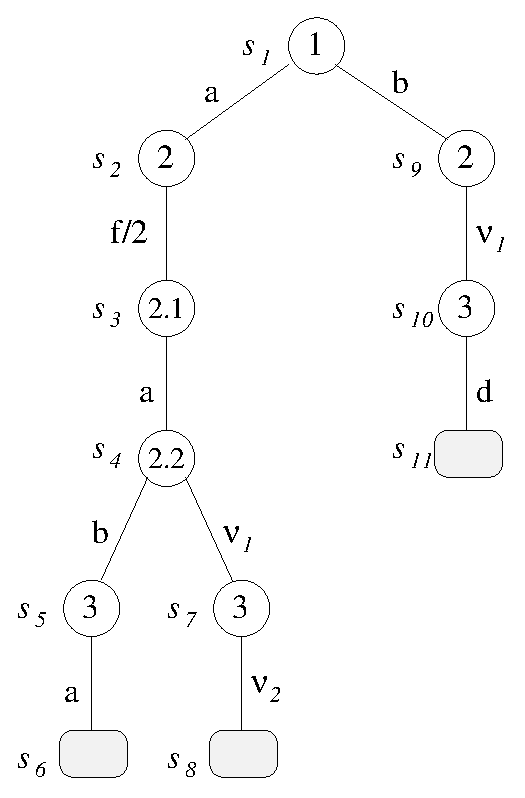
\epsfig{file=trie.eps,height=.3\textheight}
\end{tabular}
\caption{Terms Stored as a Trie}
\end{figure} 
Using a trie for storage has the advantage that discrimination can be
made on a position anywhere in a fact, and directly inserting into or
deleting from a trie is 4-5x faster than with standard dynamic code.
In addition, in trie-dynamic code, there is no distinction between the
index and the code itself, so for many sets of facts trie storage can
use much less space than standard dynamic code.  For instance,
Figure~\ref{fig:trie} shows how the prefix {\tt rt(a,f(a,...} is
shared for the first two facts.  However, trie storage comes with
tradeoffs: first, only facts can be stored in a trie; second, unlike
standard dynamic code, no ordering is preserved among the facts; and
third, duplicate facts are not supported.

In \version{} of XSB, tries that store facts may have the following
forms~\footnote{Future versions may support more types of tries}:
%
\bi
\item {\em Private, general} tries allow arbitrary terms to be
  inserted in a trie.  These tries are thread-private so that
  inserting a term in a trie $Tr$ in one thread will not be visible to
  another thread.  Although such tries are general, they have
  limitations in memory reclamation in \version{} of XSB.  If a term
  is deleted from $Tr$, memory will be reclaimed if it is safe to do
  so at the time of deletion~\footnote{That is, if no choice points
    are around that may cause backtracking into $Tr$.}; otherwise the
  space will not be reclaimed until all terms in $Tr$ are removed by
  truncating $Tr$ or until the thread exits.

\item {\em Private, associative} Associative tries are more restricted
  than general tries: an associative trie combines a {\em key} which
  can be any ground term, with a {\em value} which can be any term.
  Memory for deleted key-value pairs in an associative trie is always
  immediately reclaimed, and insert or delete operations can be faster
  for an associative trie than for a general trie.  These tries are
  private to a thread, and in addition to reclaiming memory when a
  term is deleted, memory is reclaimed when the trie is truncated or
  dropped, and when the thread exits.

\item {\em Shared, associative} tries are associative tries that are
  shared among threads.  Memory for deleted key-value pairs is always
  immediately reclaimed, and when the trie is truncated or dropped.
  \ei

\section{Examples of Using Tries}

A handle for a trie can be obtained using the {\tt trie\_create/2}
predicate.  Terms can then be inserted into or deleted from that trie,
and terms can be unified with information in the trie, as shown in the
following example:

\begin{example} \rm
First, we create a private general trie: 
{\small
\begin{verbatim}
| ?- trie_create(X,[type(prge)]).
X = 1

yes
\end{verbatim}
}
%
Next, we insert some terms into the trie
{\small
\begin{verbatim}
| ?- trie_insert(1,f(a,b)), trie_insert(1,[a,dog,walks]).

yes
\end{verbatim}
}
Now we can make arbitrary queries against the trie
{\small
\begin{verbatim}
| ?- trie_unify(1,X).

X = [a,dog,walks];

X = f(a,b);

no
\end{verbatim}
}
\noindent
Above, a general query was made, but the query could have been any
Prolog term.  Now we delete a term, and see what's left.
{\small
\begin{verbatim}
| ?- trie_delete(1,f(X,B)).

X = a
B = b

yes
| ?- trie_unify(1,X).

X = [a,dog,walks];

no
\end{verbatim}
}
\end{example}

The behavior of general tries can be constrasted with that of
associative tries as seen in the next example.
\begin{example} \rm
Now we start by creating a shared associative trie, with abbreviation
{\tt shas} using the multi-threaded engine
{\small
\begin{verbatim}
| ?- trie_create(X,[type(shas),alias(foo)]).
X = 1048577

yes
\end{verbatim}
}  \noindent
%
This time we used an alias so now we can use {\tt foo} to refer to
insert a couple of key-value pairs into the trie (we could also use
the trie handle itself) 
{\small
\begin{verbatim}
| ?- trie_insert(foo,pair(sentence(1),[a,dog,walks])), 
     trie_insert(foo,pair(sentence(2),[a,man,snores])).

yes
\end{verbatim}
} \noindent
However, inserting a general term into an associative trie throws an
error
{\small
\begin{verbatim}
| ?- trie_insert(foo,f(a,b)).
++Error[XSB/Runtime/P]: [Domain (f(a,b) not in domain pair/2)]  
in arg 2 of predicate trie_insert/2 
(Inserted term must be key-value pair in trie 1048577)
\end{verbatim}
}  \noindent
Finally, in an associative trie, if we insert a value for a key that
is already in the trie, it will {\em update} the value for that key.
{\small
\begin{verbatim}
| ?- trie_insert(foo,pair(sentence(1),[a,dog,snoress])).

yes
| ?- trie_unify(foo,pair(sentence(1),X)).
X = [a,dog,snores]

yes
\end{verbatim}
}

\end{example}

\section{Predicates for Tries} 
%
The following subsections describe predicates for inserting terms into
a trie, deleting terms from a trie, and unifying a term with terms in
a trie, predicates for creating, dropping, and truncating tries, as
well as predicates for bulk insertes into and deletes from a trie.
These predicates can apply to any type of trie, and perform full error
checking on their call arguments.  As such, they are safer and more
general than the lower-level trie predicates described in Chapter 1 of
Volume 2 of this manual.  Use of the predicates described here is
recommended for applications unless the need for speed is paramount.

\begin{description}
%
\index{aliases!tries}
\ourmoditem{trie\_create(-TrieId,+OptionList)}{trie\_create/2}{intern}
%
{\tt OptionList} allows optional parameters in the configuration of a
trie to indicate its type and whether an alias should be used.  In the
present version, {\tt OptionList} may contain the following terms
\bi
\item {\tt type(Type)} where {\tt Type} can be one of
\bi
\item {\tt prge} (private, general) maintains information that is
  accessable only to the calling thread.  No other restrictions are
  made for accessing information in a private trie.  In the
  single-threaded engine, tries are private by default.

\item {\tt pras} (private, associative) creates a private trie that
  maintains key-value pairs in a manner similar to an associative
  array, using the term {\tt pair(Key,Value)}.  Each key must be ground,
  and there may be only one value per key.

\item {\tt shas} (shared associative) creates a shared trie that
  maintains key-value pairs in a manner similar to an associative
  array, using the term {\tt pair(Key,Value)}.  Each key must be
  ground, and there may be only one value per key.  This option is
  available only in the multi-threaded engine

%\item {\tt shared(full)} Maintains information that is accessable to
%  all threads, with no restrictions on its access.  In the
%  single-threaded engine, there is no distinction between private and
%  shared tries.
\ei
\item {\tt alias(Alias)}: Allow trie {\tt TrieId} to be referred to
  via {\tt Alias} in all standard trie predicates.  {\tt Alias}
  remains active for {\tt TrieId} until it is dropped.
\ei
%
{\bf Error Cases}
\bi
\item 	{\tt TrieId} is not a variable
\bi
\item 	{\tt type\_error(variable,TrieId)}
\ei
\item 	{\tt OptionList} is a partial list or contains an option that is a variable
\bi
\item 	{\tt instantiation\_error}
\ei
\item 	{\tt OptionList} is neither a list nor a partial list
\bi
\item 	{\tt type\_error(list,OptionsList)}
\ei
\item 	{\tt OptionList} contains an option, {\tt Option} not described above
\bi
\item 	{\tt domain\_error(trie\_option,Option)}
\ei
\item An element of {\tt OptionsList} is alias(A) and A is already
  associated with an existing thread, queue, mutex or stream 
\bi
\item {\tt permission\_error(create,alias, A)}
\ei
\item An element of {\tt OptionsList} is alias(A) and A its not an atom
\bi
\item {\tt type\_error(atom,A)}
\ei
\ei

\ourmoditem{trie\_insert(+TrieIdOrAlias,Term)}{trie\_insert/2}{intern}
%
Inserts {\tt Term} into the trie denoted by {\tt TrieIdOrAlias}.  If
{\tt TrieIdOrAlias} denotes an associative trie, {\tt Term} must be of
the form {\tt pair(Key,Value)} where {\tt Key} is ground.  If {\tt
  TrieIdOrAlias} is a general trie and already contains {\tt Term},
the predicate fails (as the same term cannot be inserted multiple
times in the same trie).  Similarly, if {\tt TrieIdOrAlias} is an
associative trie and already contains a value for {\tt Key} the
predicate fails.

{\bf Error Cases}
\bi
\item 	{\tt TrieIdOrAlias} is a variable
\bi
\item 	{\tt instantiation\_error}.
\ei
\item 	{\tt TrieIdOrAlias} is not a trie id or alias
\bi
\item 	{\tt domain\_error(trie\_id\_or\_alias,TrieIdOrAlias)}
\ei
\item 	{\tt TrieIdOrAlias} denotes an associative array, and {\tt Term} 
  does not unify with {\tt pair(\_,\_)} 
\bi
\item 	{\tt domain\_error(pair/2,Term)}
\ei
\item 	{\tt TrieIdOrAlias} denotes an associative array, 
  {\tt Term = pair(Key,Value)} but {\tt Key} is not ground 
\bi
\item 	{\tt misc\_error}
\ei
\ei
%

\ourmoditem{trie\_unify(+TrieIdOrAlias,Term)}{trie\_unify/2}{intern}
%
Unifies {\tt Term} with a term in the trie denoted by {\tt
  TrieIdOrAlias}.  If {\tt TrieIdOrAlias} denotes a general trie,
successive unifications will succeed upon backtracking.  If {\tt
  TrieIdOrAlias} denotes an associative trie, {\tt Term} must be of
the form {\tt pair(Key,Value)} where {\tt Key} is ground.

{\bf Error Cases}
\bi
\item 	{\tt TrieIdOrAlias} is a variable
\bi
\item 	{\tt instantiation\_error}.
\ei
\item 	{\tt TrieIdOrAlias} is not a trie id or alias
\bi
\item 	{\tt domain\_error(trie\_id\_or\_alias,TrieIdOrAlias)}
\ei
\item 	{\tt TrieIdOrAlias} denotes an associative array, and {\tt Term} 
  does not unify with {\tt pair(\_,\_)} 
\bi
\item 	{\tt domain\_error(pair/2,Term)}
\ei
\item {\tt TrieIdOrAlias} denotes an associative array, 
  {\tt Term = pair(Key,Value)} but {\tt Key} is not ground 
\bi
\item 	{\tt misc\_error}
\ei
\ei

\ourmoditem{trie\_delete(+TrieIdOrAlias,Term)}{trie\_delete/2}{intern}
%
Deletes a term unifying with {\tt Term} from the trie denoted by {\tt
  TrieIdOrAlias}.  {\tt TrieIdOrAlias} denotes a general trie, all
such terms can be deleted upon backtracking.  If {\tt TrieIdOrAlias}
denotes an associative trie, {\tt Term} must be of the form {\tt
  pair(Key,Value)} where {\tt Key} is ground.  In either case, if {\tt
  TrieIdOrAlias} does not contain a term unifying with {\tt Term} the
preicate fails.

{\bf Error Cases}
\bi
\item 	{\tt TrieIdOrAlias} is a variable
\bi
\item 	{\tt instantiation\_error}.
\ei
\item 	{\tt TrieIdOrAlias} is not a trie id or alias
\bi
\item 	{\tt domain\_error(trie\_id\_or\_alias,TrieIdOrAlias)}
\ei
\item 	{\tt TrieIdOrAlias} denotes an associative array, and {\tt Term} 
  does not unify with {\tt pair(\_,\_)} 
\bi
\item 	{\tt domain\_error(pair/2,Term)}
\ei
\item {\tt TrieIdOrAlias} denotes an associative array, 
  {\tt Term = pair(Key,Value)} but {\tt Key} is not ground 
\bi
\item 	{\tt misc\_error}
\ei
\ei
%
\ourmoditem{trie\_truncate(+TrieIdOrAlias)}{trie\_truncate/1}{intern}
%
Removes all terms from {\tt TrieIdOrAlias}, but does not change any of
its properties (e.g. the type of the trie or its aliases).  

{\bf Error Cases}
\bi
\item 	{\tt TrieIdOrAlias} is a variable
\bi
\item 	{\tt instantiation\_error}.
\ei
\item 	{\tt TrieIdOrAlias} is not a trie id or alias
\bi
\item 	{\tt domain\_error(trie\_id\_or\_alias,TrieIdOrAlias)}
\ei
\ei

\ourmoditem{trie\_drop(+TrieIdOrAlias)}{trie\_drop/1}{intern}
%
Drops {\tt TrieIdOrAlias}.  {\tt trie\_drop/1} not only removes all
terms from {\tt TrieIdOrAlias}, but also removes information about its
type and any aliases the trie may have.

{\bf Error Cases}
\bi
\item 	{\tt TrieIdOrAlias} is a variable
\bi
\item 	{\tt instantiation\_error}.
\ei
\item 	{\tt TrieIdOrAlias} is not a trie id or alias
\bi
\item 	{\tt domain\_error(trie\_id\_or\_alias,TrieIdOrAlias)}
\ei
\ei

\ourmoditem{trie\_bulk\_insert(+TrieIdOrAlias,+Generator)}{trie\_bulk\_insert/2}{intern}
% 
Used to insert multiple terms into the trie denoted by {\tt
  TrieIdOrAlias}.  {\tt Generator} must be a callable term.  Upon
backtracking through {\tt Generator} its first argument should
successively be instantiated to the terms to be interned in {\tt
  TrieIdOrAlias}.  When inserting many terms into a general trie, {\tt
  trie\_bulk\_insert/2} is faster than repeated calls to {\tt
  trie\_insert/2} as it does not need to make multiple checks that the
choice point stack is free of failure continuations that point into
the {\tt TrieIdOrAlias} trie.  For associative tries, {\tt
  trie\_bulk\_insert/2} can also be faster as it needs to perform
fewer error checks on the arguments of the insert.

\begin{example} \rm
Given the predicate 
\begin{verbatim}
bulk_create(p(One,Two,Three),N):- 
     for(One,1,N),
     for(Two,1,N),
     for(Three,1,N).
\end{verbatim}
and a general trie {\tt Trie}, the goal 
\begin{center}
   {\tt ?- trie\_bulk\_insert(Trie,bulk\_create(\_Term,N))} 
\end{center}
will add $N^3$ terms to {\tt Trie}.
\end{example}

{\bf Error Cases}
\bi
\item 	{\tt TrieIdOrAlias} is a variable
\bi
\item 	{\tt instantiation\_error}.
\ei
\item 	{\tt TrieIdOrAlias} is not a trie id or alias
\bi
\item 	{\tt domain\_error(trie\_id\_or\_alias,TrieIdOrAlias)}
\ei
\item   {\tt Generator} is not a compound term
\bi
\item   {\tt type\_error(compound,Generator)}
\ei
\item 	{\tt TrieIdOrAlias} denotes an associative array, and {\tt Generator} 
  does not unify with {\tt pair(\_,\_)} 
\bi
\item 	{\tt domain\_error(pair/2,Term)}
\ei
\item {\tt TrieIdOrAlias} denotes an associative array, and {\tt
  Generator} succeeds with a term that unifies with {\tt
  pair(Key,Value)} and {\tt Key} is not ground 
\bi
\item 	{\tt misc\_error}
\ei
\ei

\ourmoditem{trie\_bulk\_delete(+TrieIdOrAlias,Term)}{trie\_bulk\_delete/2}{intern}
% 
Deletes all terms that unify with {\tt Term} from {\tt TrieIdOrAlias}.
If {\tt TrieIdOrAlias} denotes an associative trie, the key of the key
value pair need {\em not} be ground.

\begin{example}\label{ex:bulk-delete} \rm
For the trie in the previous example, the goal 
\begin{center}
{\tt ?-  trie\_bulk\_delete(Trie,p(1,\_,\_))} 
\end{center}
will delete the $N^2$ terms that unify with {\tt p(1,\_,\_)} from {\tt TrieIdOrAlias}.
\end{example}

{\bf Error Cases}
\bi
\item 	{\tt TrieIdOrAlias} is a variable
\bi
\item 	{\tt instantiation\_error}.
\ei
\item 	{\tt TrieIdOrAlias} is not a trie id or alias
\bi
\item 	{\tt domain\_error(trie\_id\_or\_alias,TrieIdOrAlias)}
\ei
\ei

\ourmoditem{trie\_bulk\_unify(+TrieIdOrAlias,\#Term,-List)}{trie\_bulk\_unify/3}{intern}
% 
Returns in {\tt List} all terms in {\tt TrieIdOrAlias} that unify with
{\tt Term}.  If {\tt TrieIdOrAlias} denotes an associative trie, the
key of the key value pair need {\em not} be ground.

This predicate is useful for two reasons.  First, it provides a safe
way to backtrack through an associative trie while maintaining the
memory management and concurrency properties of associative tries.
Second, it enforces read consistency for {\tt TrieIdOrAlias},
regardless of whether the trie is private or shared, general or
associative.

\begin{example} \rm
Continuing from Example~\ref{ex:bulk-delete} the goal
\begin{center}
{\tt ?-  trie\_bulk\_unify(Trie,X),List} 
\end{center}
will return the the $N^3 - N^2$ terms still in {\tt TrieIdOrAlias}.
\end{example}

{\bf Error Cases}
\bi
\item 	{\tt TrieIdOrAlias} is a variable
\bi
\item 	{\tt instantiation\_error}.
\ei
\item 	{\tt TrieIdOrAlias} is not a trie id or alias
\bi
\item 	{\tt domain\_error(trie\_id\_or\_alias,TrieIdOrAlias)}
\ei
\item 	{\tt List} is not a variable
\bi
\item 	{\tt type\_error(variable,List)}.
\ei
\ei

\ourmoditem{trie\_property(?TrieOrAlias,?Property)}{trie\_property/2}{intern}
%
If {\tt TrieOrAlias} is instantiated, unifies {\tt Property} with
current properties of the trie; if {\tt TrieOrAlias} is a variable,
backtracks through all the current tries whose properties unify with
{\tt Property}.  In the MT engine, {\tt thread\_property/2} accesses
only tries private to the calling thread and shared tries; however
note that there is no guarantee that that the information returned
about shared tries will be valid, due to concurrency
issues~\footnote{{\tt trie\_property/2} is not yet implemented for
  shared tries.}.

Currently {\tt Property} can have the form 
\bi
\item {\tt type(Type)}: where {\tt Type} is the type of the trie.
%
\item {\tt alias(Alias)}: if the trie has an alias {\tt Alias}
\ei

{\bf Error Cases}
%
\bi
\item {\tt TrieOrAlias} is neither a variable nor an XSB trie id
  nor an alias
\bi
\item {\tt domain\_error(trie, TrieOrAlias)}
\ei
\item {\tt TrieOrAlias} is not associated with a valid trie
\bi
\item {\tt existence\_error(trie, TrieOrAlias)}
\ei
\ei

%\ouritem{trie\_property(+TrieIdOrAlias,Property)}
%\index{\texttt{trie\_property/2}}
%
\end{description}


\chapter{Hooks} \label{hooks}

Sometimes it is useful to let the user application catch certain
events that occur during XSB execution. For instance, when the user
asserts or retracts a clause, etc.
XSB has a general mechanism by which the
user program can register \emph{hooks} to handle certain supported
events. All the predicates described below must be imported from {\tt
xsb\_hook}.


\section{Adding and Removing Hooks}

A hook in XSB can be either a 0-ary predicate or a unary predicate.
A 0-ary hook is called without parameters and unary hooks are called with
one parameter. The nature of the parameter depends on the type of the hook,
as described in the next subsection.


\begin{description}
\ouritem{add\_xsb\_hook(+HookSpec)} \index{{\tt add\_xsb\_hook/1}} 

This predicate registers a hook; it must be imported from {\tt xsb\_hook}.
{\tt HookSpec} has the following format:
%%
\begin{quote}
 {\tt
   hook-type(your-hook-predicate(\_))
   }
\end{quote}
%%
or, if it is a 0-ary hook:
%%
\begin{quote}
  {\tt
   hook-type(your-hook-predicate)
   }  
\end{quote}
%%
For instance, 
%%
\begin{verbatim}
    :- add_xsb_hook(xsb_assert_hook(foobar(_))).
\end{verbatim}
%%
registers the hook {\tt foobar/1} as a hook to be called when XSB
asserts a clause. Your program must include
clauses that define {\tt foobar/1}, or else an error will result.

The predicate that defines the hook type must be imported from {\tt
  xsb\_hook}:
%%
\begin{verbatim}
    :- import xsb_assert_hook/1 from xsb_hook.  
\end{verbatim}
%%
or {\tt add\_xsb\_hook/1} will issue an error.

\ouritem{remove\_xsb\_hook(+HookSpec)} \index{{\tt remove\_xsb\_hook/1}}

Unregisters the specified XSB hook; imported from {\tt xsb\_hook}. For
instance,
%%
\begin{verbatim}
    :- remove_xsb_hook(xsb_assert_hook(foobar(_))).
\end{verbatim}
%%
As before, the predicate that defines the hook type must be imported from
{\tt xsb\_hook}.
\end{description}


\section{Hooks Supported by XSB}

The following predicates define the hook types supported by XSB. They must
be imported from {\tt xsb\_hook}.

\begin{description}
\ouritem{xsb\_exit\_hook(\_)} \index{{\tt xsb\_exit\_hook/1}}

These hooks are called just before XSB exits. You can register as many
hooks as you want and all of them will be called on exit (but the order of
the calls is not guaranteed). Exit hooks are all 0-ary and must be registered
as such:
%%
\begin{verbatim}
    :- add_xsb_hook(xsb_exit_hook(my_own_exit_hook)).
\end{verbatim}
%%


\ouritem{xsb\_assert\_hook(\_)} \index{{\tt xsb\_assert\_hook/1}}

These hooks are called whenever the program asserts a clause. An assert
hook must be a unary predicate, which expects the clause
being asserted as a parameter. For instance,
%%
\begin{verbatim}
    :- add_xsb_hook(xsb_assert_hook(my_assert_hook(_))).
\end{verbatim}
%%
registers {\tt my\_assert\_hook/1} as an assert hook. One can register
several assert hooks and all of them will be called (but the order is not
guaranteed).

\ouritem{xsb\_retract\_hook(\_)} \index{{\tt xsb\_retract\_hook/1}}

These hooks are called whenever the program retracts a clause. A retract
hook must be a unary predicate, which expects as a parameter a list of the
form {\tt [Head,Body]}, which represent the head and the body parts of the
clause being retracted. As with assert hooks, any number of retract hooks
can be registered and all of them will be called in some order.

\end{description}


%%% Local Variables: 
%%% mode: latex
%%% TeX-master: "manual1"
%%% End: 

\chapter{Debugging} \label{debugging}
%====================================
\index{debugger}
\index{tracing|(}
\section{Prolog-style Tracing and Debugging}
%===========================
\index{high-level tracing} \index{tracing!Prolog Programs}
%
XSB supports a version of the Byrd four-port debugger for interactive
debugging and tracing of Prolog code.  In this release (\version), it
does not work very well when debugging code involving tabled
predicates~\footnote{The current version of XSB's Prolog debugger does
  not include exceptions as a debugging port.}.  If one only creeps
(see below), the tracing can provide some useful information.  For
programs that involve large amounts of tabling forest-view tracing can
be used (Section~\ref{sec:forest-trace}).
To turn on tracing, use {\tt trace/0}, {\tt trace/1}, or {\tt trace/2}.  To
turn tracing off, use {\tt notrace/0}.

\begin{description}
\repeatstandarditem{trace}{trace/0}
\standarditem{notrace}{notrace/0}

When tracing is on, the system will print a message each time a
predicate is:
\begin{enumerate} \index{debugger!ports}
\item initially entered (Call), 
\item successfully returned from (Exit), 
\item failed back into (Redo), and
\item completely failed out of (Fail).  
\end{enumerate}
When debugging interactively, a message may be printed and tracer
stopped and prompts for input.  (See the predicates {\tt show/1} and
{\tt leash/1} described below to modify what is traced and when the
user is prompted.)

In addition to single-step tracing, the user can set spy points to
influence how the tracing/debugging works.  A spy point is set using
{\tt spy/1}.  Spy points can be used to cause the system to enter the
tracer when a particular predicate is entered. Also the tracer allows
``leaping'' from spy point to spy point during the debugging process.
%
The debugger also has profiling capabilities, which can measure the cpu
time spent in each call. The cpu time is measured only down to 0.0001-th
of a second.
g
When the tracer prompts for input, the user may enter a return, or a single
character followed by a return, with the following meanings:
\bi
\index{trace!options}
\item{\tt c, <CR>}: {\em Creep}~ Causes the system to single-step to
  the next port (i.e.\ either the entry to a traced predicate called
  by the executed clause, or the success or failure exit from that
  clause).
\item{\tt a}: {\em Abort}~ \index{abort!trace facility} Causes execution to abort
  and control to return to the top level interpreter.
\item{\tt b}: {\em Break}~ Calls the evaluable predicate {\em break},
  thus invoking recursively a new incarnation of the system
  interpreter.  The command prompt at break level $n$ is
  \begin{center}
    {\tt $n$: \tt ?-}
  \end{center}
  The user may return to the previous break level by entering the system
  end-of-file character (e.g.\ {\tt ctrl-D}), or typing in the atom 
  {\tt end\_of\_file}; or to the top level interpreter by typing in
  {\tt abort}.
\item{\tt f}: {\em Fail}~ Causes execution to fail, thus transferring
  control to the Fail port of the current execution.
\item{\tt h}: {\em Help}~ Displays the table of debugging options.
\item{\tt l}: {\em Leap}~ Causes the system to resume running the
  program, only stopping when a spy-point is reached or the program
  terminates.  This allows the user to follow the execution at a
  higher level than exhaustive tracing.
\item{\tt n}: {\em Nodebug}~ Turns off debug mode.
\item{\tt r}: {\em Retry (fail)}~ Transfers to the Call port of the current
  goal.  Note, however, that side effects, such as database modifications
  etc., are not undone.
\item{\tt s}: {\em Skip}~ Causes tracing to be turned off for the entire
  execution of the procedure.  Thus, nothing is seen until control comes
  back to that procedure, either at the Success or the Failure port.
\item{\tt q}: {\em Quasi-skip} This is like Skip except that it does not mask
  out spy points.
\item{\tt S}: {\em Verbose skip}~ Similar to {\tt Skip} mode, but trace
  continues to be printed. The user is prompted again when the current call
  terminates with success or failure.  This can be used to obtain a full
  trace to the point where an error occurred or for code profiling. (See
  more about profiling below.)
\item{\tt e}: {\em Exit}~ Causes immediate exit from \ourprolog\ back to the
  operating system.
\ei
%/* TLS: it seems like there may not be much use for the non-queryable trace/1 */

\standarditem{trace(+Filename,+option)}{trace/2}
\index{trace!logging}
%\index[pred]{\texttt{trace/1}}
%\index{\texttt{trace/1}}
%
{\tt trace/2} is like {\tt trace/0} except that it is non-interactive
and dumps trace information into a log file, {\tt Filename}.
Currently the only supported option is \texttt{log}.  However, the log
is written in the form of Prolog facts, which can be loaded
queried. The format of the facts is:
%% 
\begin{verbatim}
xsb_tracelog(CallId,CallNum,PortType,ParentCallNum,DepthOfCall,CurrentCall,Time)
\end{verbatim}
%% 
where \texttt{CallId} is an identifier generated when XSB encounters a
new top-level call. This identifier remains the same for all subgoals
called while tracing that top-level call.
\bi
\item \texttt{CallNum} is a generated number to show the nesting of
  the calls being traced. It is the same number that the user sees
  when tracing interactively.
%
\item \texttt{PortType} is \texttt{'Call'}, \texttt{'Redo'},
  \texttt{'Exit'}, or \texttt{'Fail'}.  
\item \texttt{ParentCallNum} is the call number of the parent call.
%
\item \texttt{DepthOfCall} is the nesting depth of the current call
  with respect to its ancestor calls.  
%
\item \texttt{CurrentCall} is the call being traced
%
\item \texttt{Time} is the CPU time it took to execute
  \texttt{CurrentCall}. On \texttt{'Call'} and \texttt{'Redo'},
  \texttt{Time} is always 0 --- it has a meaningful value only for the
  \texttt{'Exit'} and \texttt{'Fail'} log entries. 
\end{itemize}
It should be noted that when calls are delayed due to the well-founded
negation computation of because of the \texttt{when/2} primitive, the
parent call might be off in some cases. However, the parent property
repairs itself for subsequent calls.

`The name of the predicate (\texttt{xsb\_tracelog}) used for logging
can be changed by asserting it into the predicate
\texttt{debug\_tracelog\_predicate/1}, which should be imported from
\texttt{usermod}. For instance,
%% 
\begin{verbatim}
   :- import debug_tracelog_predicate/1 from usermod.
   ?- assert(debug_tracelog_predicate(foobar)).
\end{verbatim}
%% 

\standarditem{spy(Preds)}{spy/1}
    where {\tt Preds} is a spy specification or a list of such
    specifications, and must be instantiated. This predicate sets spy
    points (conditional or unconditional) on predicates.  A spy
    specification can be of several forms. Most simply, it is a term
    of the form $P$/$N$, where $P$ is a predicate name and $N$ its
    arity.  Optionally, only a predicate name can be provided, in
    which case it refers to all predicates of any arity currently
    defined in {\tt usermod}.  It may optionally may be prefixed by a
    module name, e.g.  $ModName$:$P$/$N$. (Again, if the arity is
    omitted, the specification refers to all predicates of any arity
    with the given name currently defined in the given module.)  A spy
    specification may also indicate a conditional spy point. A
    conditional spy specification is a Prolog rule, the head
    indicating the predicate to spy, and the body indicating
    conditions under which to spy. For example, to spy the predicate
    p/2 when the first argument is not a variable, one would write:
    $spy (p(X,\_):-nonvar(X)).$ (Notice that the parentheses around
    the rule are necessary). The body may be empty, i.e., the rule may
    just be a fact.  The head of a rule may also be prefixed (using
    $:$) with a module name. One should not put both conditional and
    unconditional spy points on the same predicate.

\standarditem{nospy(Preds)}{nospy/1}
    where {\tt Preds} is a spy specification, or a list of such
    specifications, and must be instantiated at the time of call.  What
    constitutes a spy specification is described above under {\tt spy}.
    {\tt nospy} removes spy points on the specified predicates. If a
    specification is given in the form of a fact, all conditional spy points
    whose heads match that fact are removed.

\standarditem{debug}{debug/0}
    Turns on debugging mode.
    This causes subsequent execution of predicates with trace or spy
    points to be traced, and is a no-op if there are no such predicates.
    The predicates {\tt trace/0}, {\tt trace/1}, \texttt{trace/2},  and {\tt spy/1} cause debugging mode
    to be turned on automatically.

\standarditem{nodebug}{nodebug/0}
    Turns off debugging mode.  This causes trace and spy points to be ignored.

\standarditem{debugging}{debugging/0}
    Displays information about whether debug mode is on or not, and lists
    predicates that have trace points or spy points set on them.

\standarditem{debug\_ctl(option,value)}{debug\_ctl/2}
   {\tt debug\_ctl/2} performs debugger control functions as described below.
   These commands can be entered before starting a trace or inside the trace.
   The latter can be done by responding with ``{\tt b}'' at the prompt,
   which recursively invokes an XSB sub-session. At this point, you can
   enter the debugger control commands and type \verb|end_of_file.| This
   returns XSB back to the debugger prompt, but with new settings.
   %%
   \begin{enumerate}
   \item {\tt debug\_ctl(prompt, off)} Set non-interactive mode globally.
     This means that trace will be printed from start to end, and the user
     will never be prompted during the trace.
    \item {\tt debug\_ctl(prompt, on)} 
      Make tracing/spying interactive.
    \item {\tt debug\_ctl(profile, on)}  
      Turns profiling on. This means that each time a call execution
      reaches the {\tt Fail} or {\tt Exit} port, CPU time spent in that
      call will be printed. The actual call can be identified by locating a
      {\tt Call}  prompt that has the same number as the ``cpu time''
      message.
    \item {\tt debug\_ctl(profile, off)}  
      Turns profiling off.
    \item {\tt debug\_ctl(redirect, +File)} 
      Redirects debugging output to a file. This also includes program output,
      errors and warnings.
      Note that usually you cannot see the contents of {\tt +File} until it
      is closed, {\it i.e.}, until another redirect operation is performed
      (usually {\tt debug\_ctl(redirect, tty)}, see next).
    \item {\tt debug\_ctl(redirect, tty)}     
      Attaches the previously redirected debugging, error, program output,
      and warning streams back to the user terminal.
    \item {\tt debug\_ctl(show, +PortList)}  
      Allows the user to specify at which ports should trace messages be
      printed. {\tt PortList} must be a list of port names, i.e., a sublist
      of ['Call', 'Exit', 'Redo', 'Fail']. 
    \item {\tt debug\_ctl(leash, +PortList)}  
      Allows the user to specify at which ports the tracer should stop
      and prompt the user for direction.  {\tt PortList} must be a list of
      port names, i.e., a sublist of ['Call', 'Exit', 'Redo', 'Fail'].  Only
      ports that are {\tt show}-n can be {\tt leash}-ed. 
    \item {\tt debug\_ctl(hide, +PredArityPairList)}  
      The list must be of the form {\tt [P1/A1, P2/A2, ...]}, {\it i.e.},
      each either must specify a predicate-arity pair. Each predicate on
      the list will become non-traceable. That is, during the trace, each
      such predicate will be treated as an black-box procedure, and trace
      will not go into it.
    \item {\tt debug\_ctl(unhide, ?PredArityPairList)} If the list is a
      predicate-arity list, every predicate on that list will become
      traceable again. Items in the list can contain variables. For
      instance, {\tt debug\_ctl(unhide, [\_/2])} will make all 2-ary that
      were previously made untraceable traceable again.  As a special case,
      if {\tt PredArityPairList} is a variable, all predicates previously
      placed on the ``untraceable''-list will be taken off.
    \item {\tt debug\_ctl(hidden, -List)}
      This returns the list of predicates that the user said should not be
      traced.
   \end{enumerate}
   %%
\end{description}


\section{Low-Level Tracing}
%--------------------------------------------------
\index{low-level tracing} \index{tracing!low-level}

XSB also provides a facility for low-level tracing of execution.  This
can be activated by invoking the emulator with the {\tt -T} option
(see Section~\ref{sec:EmuOptions}), or through the predicate {\tt
  trace/0}.  \stdrefindex{\$trace/0} It causes trace information to
be printed out at every call (including those to system trap
handlers).  The volume of such trace information can very become large
very quickly, so this method of tracing is not recommended in general.

\bigskip

XSB debugger also provides means for the low-level control of what
must be traced. Normally, various standard predicates are masked out
from the trace, since these predicates do not make sense to the
application programmer.  However, if tracing below the application
level is needed, you can retract some of the facts specified in the
file {\tt syslib/debugger\_data.P} (and in some cases assert into
them). All these predicates are documented in the header of that
file. Here we only mention the four predicates that an XSB developer
is more likely to need. To get more trace, you should retract from the
first three predicates and assert into the last one.
%%
\begin{itemize}
\item {\tt hide\_this\_show(Pred,Arity)}: specifies calls (predicate name and
  arity) that the debugger should {\tt not} show at the prompt. However,
  the evaluation of this hidden call {\tt is} traced.
\item {\tt hide\_this\_hide(Pred,Arity)}: specifies calls to hide. Trace
  remains off while evaluating those predicates. Once trace is off, there
  is no way to resume it until the hidden predicate exits or fails.
\item  {\tt show\_this\_hide(Pred,Arity)}: calls to show at the
  prompt. However, trace is switched off right after that.
\item  {\tt trace\_standard\_predicate(Pred,Arity)}: Normally trace doesn't
  go inside standard predicates ({\it i.e.}, those specified in
  {\tt syslib/std\_xsb.P}. If you need to trace some of those, you must
  {\tt assert} into this predicate.
\end{itemize}
%%
In principle, by retracting all facts from the first three predicates and
asserting enough facts into the last one, it is possible to achieve the
behavior that approximates the {\tt -T} option. However, unlike {\tt -T},
debugging can be done interactively. This does not obviate {\tt -T},
however. First, it is easier to use {\tt -T} than to issue multiple asserts
and retracts. Second, {\tt -T} can be used when the error occurs early on,
before the moment when XSB shows its first prompt.

%-----------------------------------------------------------------------------
\newcommand{\mif}{\mbox{ :- }}
\newcommand{\cS}{{\cal S}}
\newcommand{\ctrace}{{\tt logforest}}

\section{Analyzing the Execution of Tabled Programs} \label{sec:forest-trace}
%
The sort of tracing and debugging described in previous sections has
proven useful for Prolog programs for 30 or more years.  However, when
tabling is added to Prolog, things change.  First, as described in
Chapter~\ref{chap:TablingOverview}, tabling can be used to find the
least fixed point of mutually recursive predicates.  Operationally,
this requires the ability to suspend one computation path and to
resume another.  The addition of tabled negation for the well-founded
semantics also requires the ability to delay negative goals whose only
proof may be involved in a loop through negation and to simplify these
goals once their truth value has become known. Furthermore, a tabled
subgoal has different states: it may be {\em new}; it may be {\em
  incomplete} so that new answers might be derived for it; or {\em
  completed} so that the answers may simply be read from the table.
In short, tabling, which can execute much more general programs than
Prolog and can use the stronger well-founded semantics, requires a
more complex set of operations than Prolog's SLDNF so that debugging
and tracing is correspondingly more complex.  Thus, while the 4-port
debugger may be useful for programs that involve just a few tabled
predicates, it may not be useful for programs that heavily use tabling
for complex recursions, non-monotinic reasoning or other purposes.

There is currently no standard approach to debugging tabled programs.
One possible approach would be to extend the 4-port debugger to
include other ports for tabling operations.  Such extensions have not
yet been explored, and whether the paradigm of n-port debugging can be
extended to full tabling so that it can be useful to programmers is an
open question.  Another approach would be use the declarative approach
of {\em justification} \cite{GuRR01,PGDRR04} to explain why
derivations were or were not made.  XSB does in fact have a
justification package but it is not currently robust enough to be
recommended for general use.  Below we present the {\tt \ctrace}
approach.

\subsection{Tracing a tabled evaluation through forest logging}
%
While the operations used for tabling are more complex than those of
SLDNF, they have a clear formal operational semantics through SLG and
the forest-of-trees model.  We recall this model briefly below for a
definite program but assume a background knowledge of tabled logic
programming (see, for instance~\cite{SwiW10}).

\begin{example} \rm 
Figure~\ref{fig:local} shows a program fragment along with an SLG
forest for the query {\tt ?- reach(1,Y)} to the the right-recursive
tabled predicate {\tt reach/1}.  An SLG forest consists of an SLG tree
for each tabled subgoal $S$: this tree has root $S \mif{} S$.  In a
definite program an SLG tree represents resolution of program clauses
and answers to prove $S$.  In Figure~\ref{fig:local} each non-root
node of the form $K. N$ where $N = (S \mif{} Goals)\theta$ is a clause
in which the bindings to a subgoal $S$ are maintained in $S\theta$,
the goals remaining to prove $S$ are in $Goals\theta$, and the order
of creation of $N$ within the tabled evaluation is represented by a
number, $K$ (local scheduling is used in this example).  Children of a
root node are obtained through resolution of a tabled subgoal against
program clauses.  Children of non-root nodes are obtained through
answer clause resolution, if the left most selected literal is tabled
(e.g. children of node 3 or 11 in the tree for {\tt reach(1,Y)}), or
through program clause resolution if the leftmost selected literal is
not tabled (e.g. children of nodes 2 and 18 in the tree for {\tt
  reach(1,Y)}).  Nodes that have empty {\em Goals} are termed {\em
  answers}.
%
\begin{figure}[htbp]
\centering
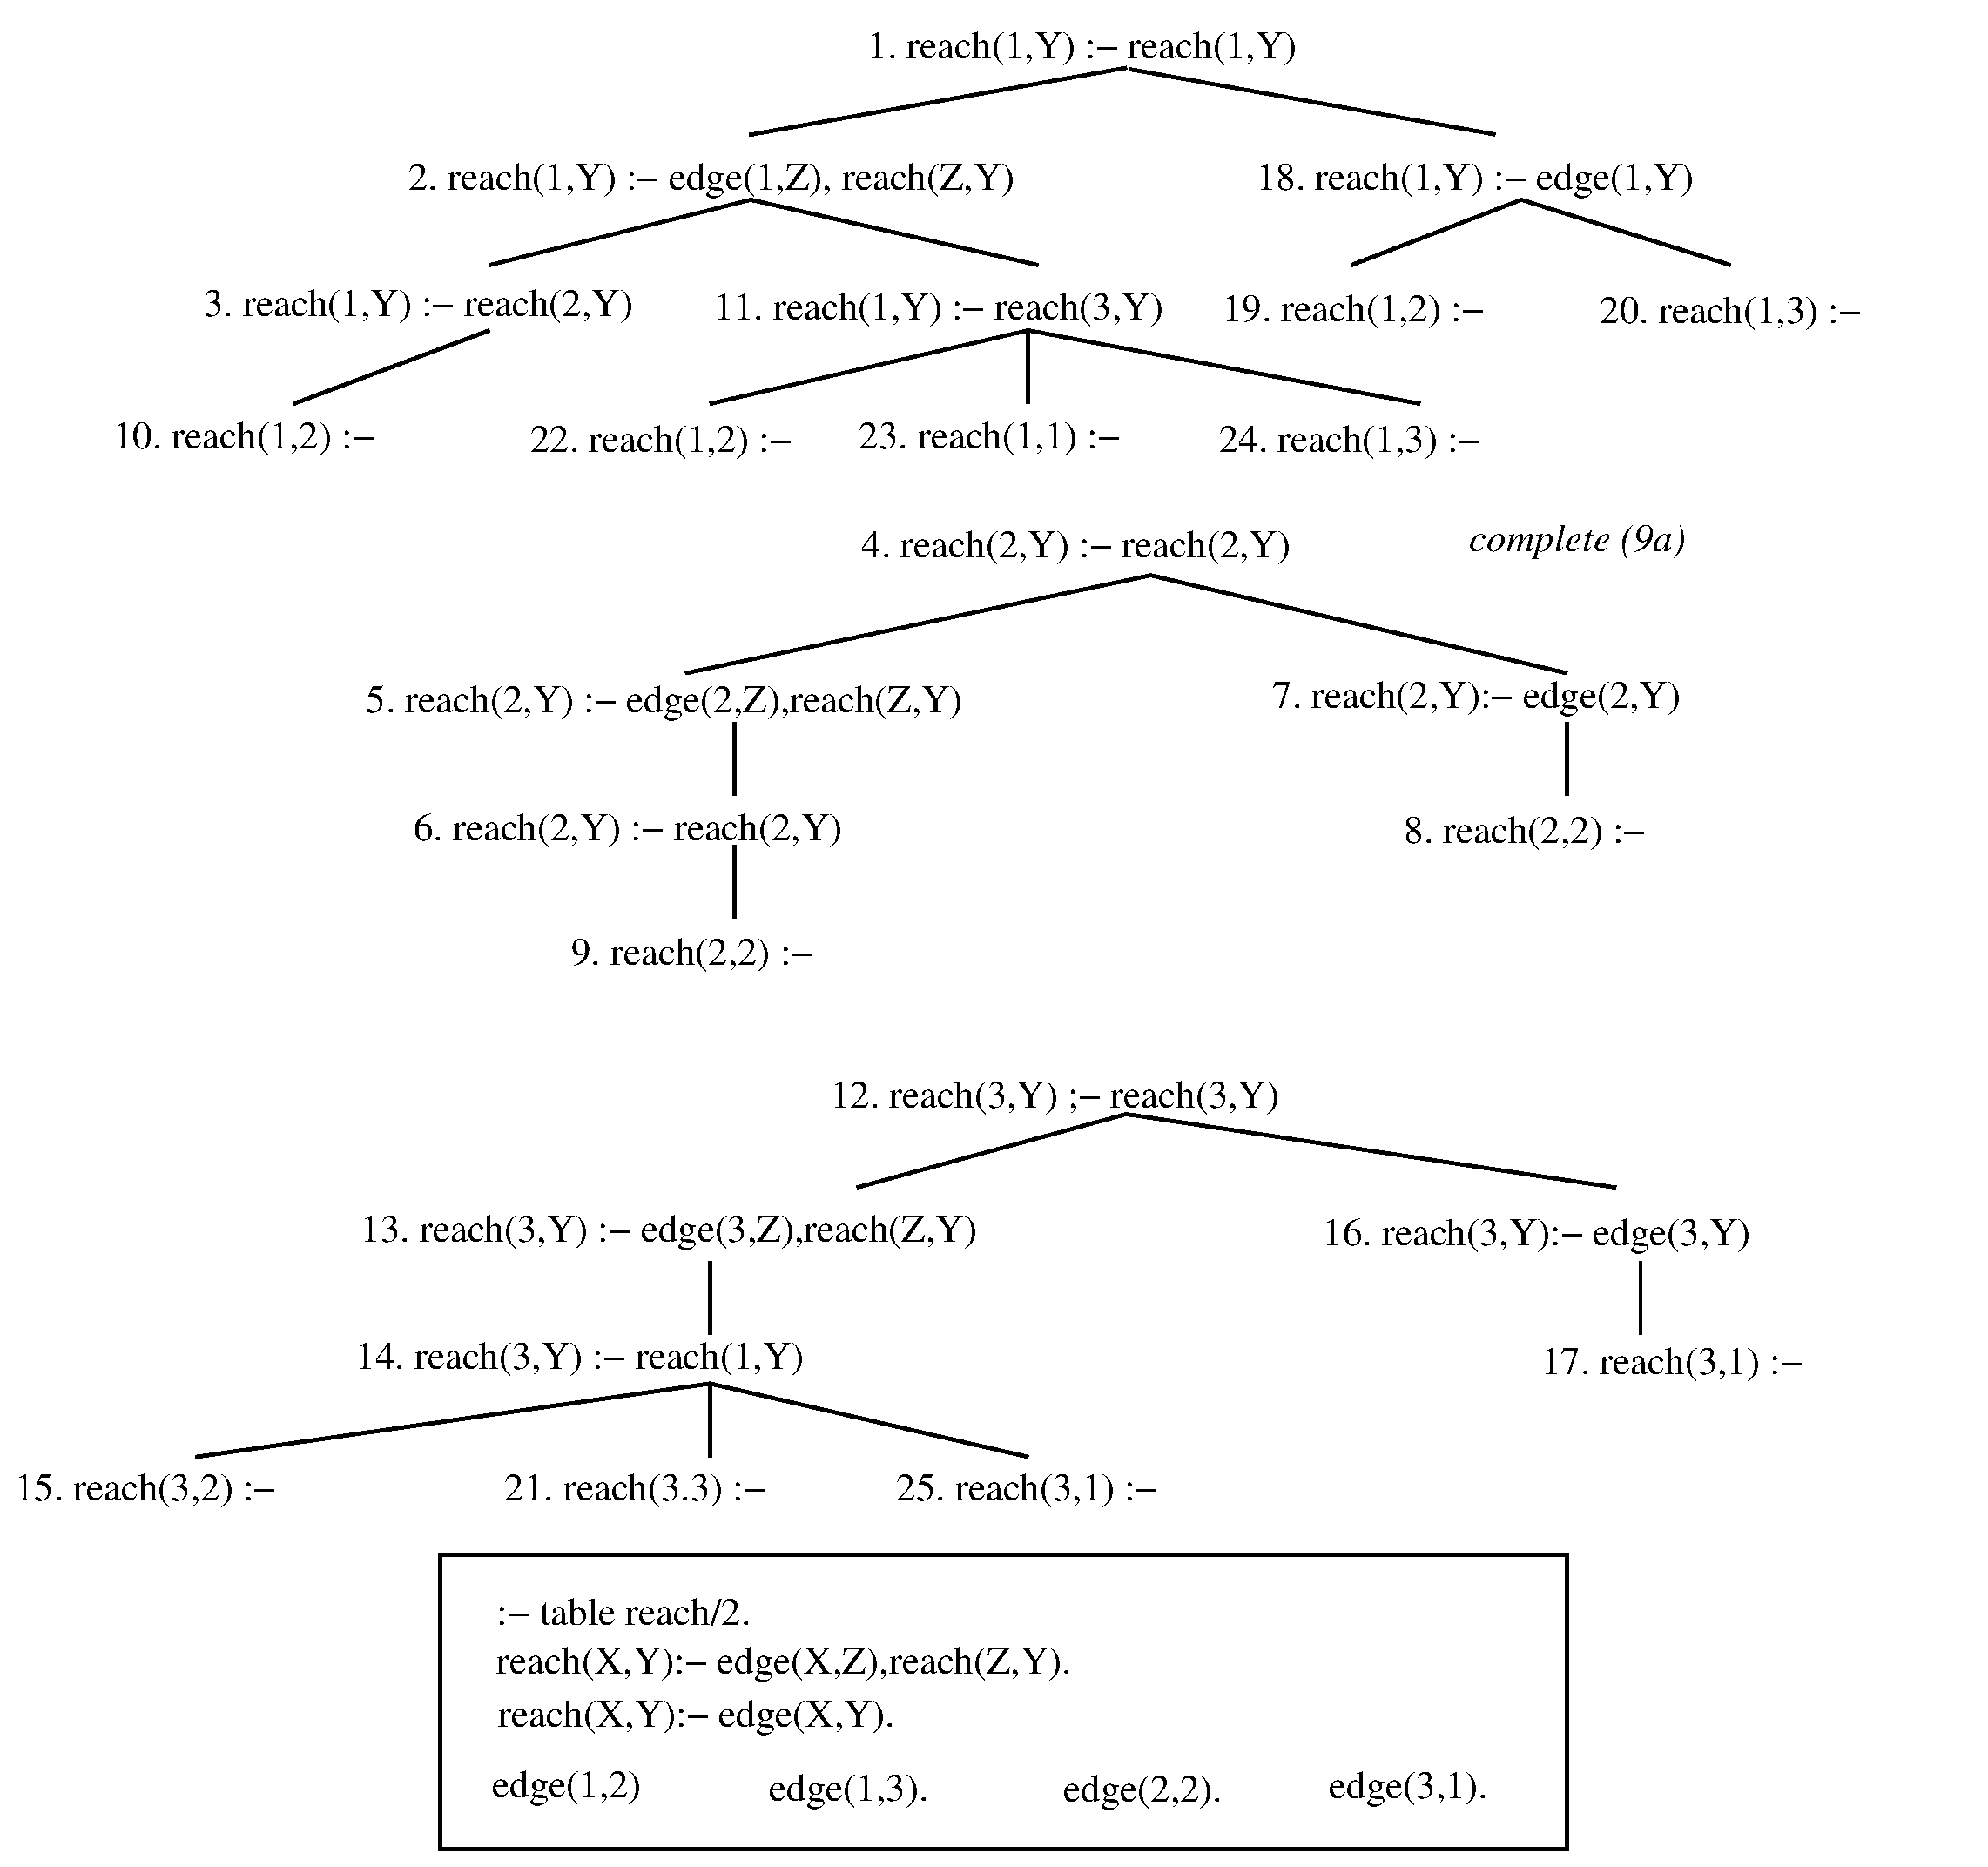
\includegraphics[width=.99\textwidth]{slg-forest-local}
%%\mbox{
%%{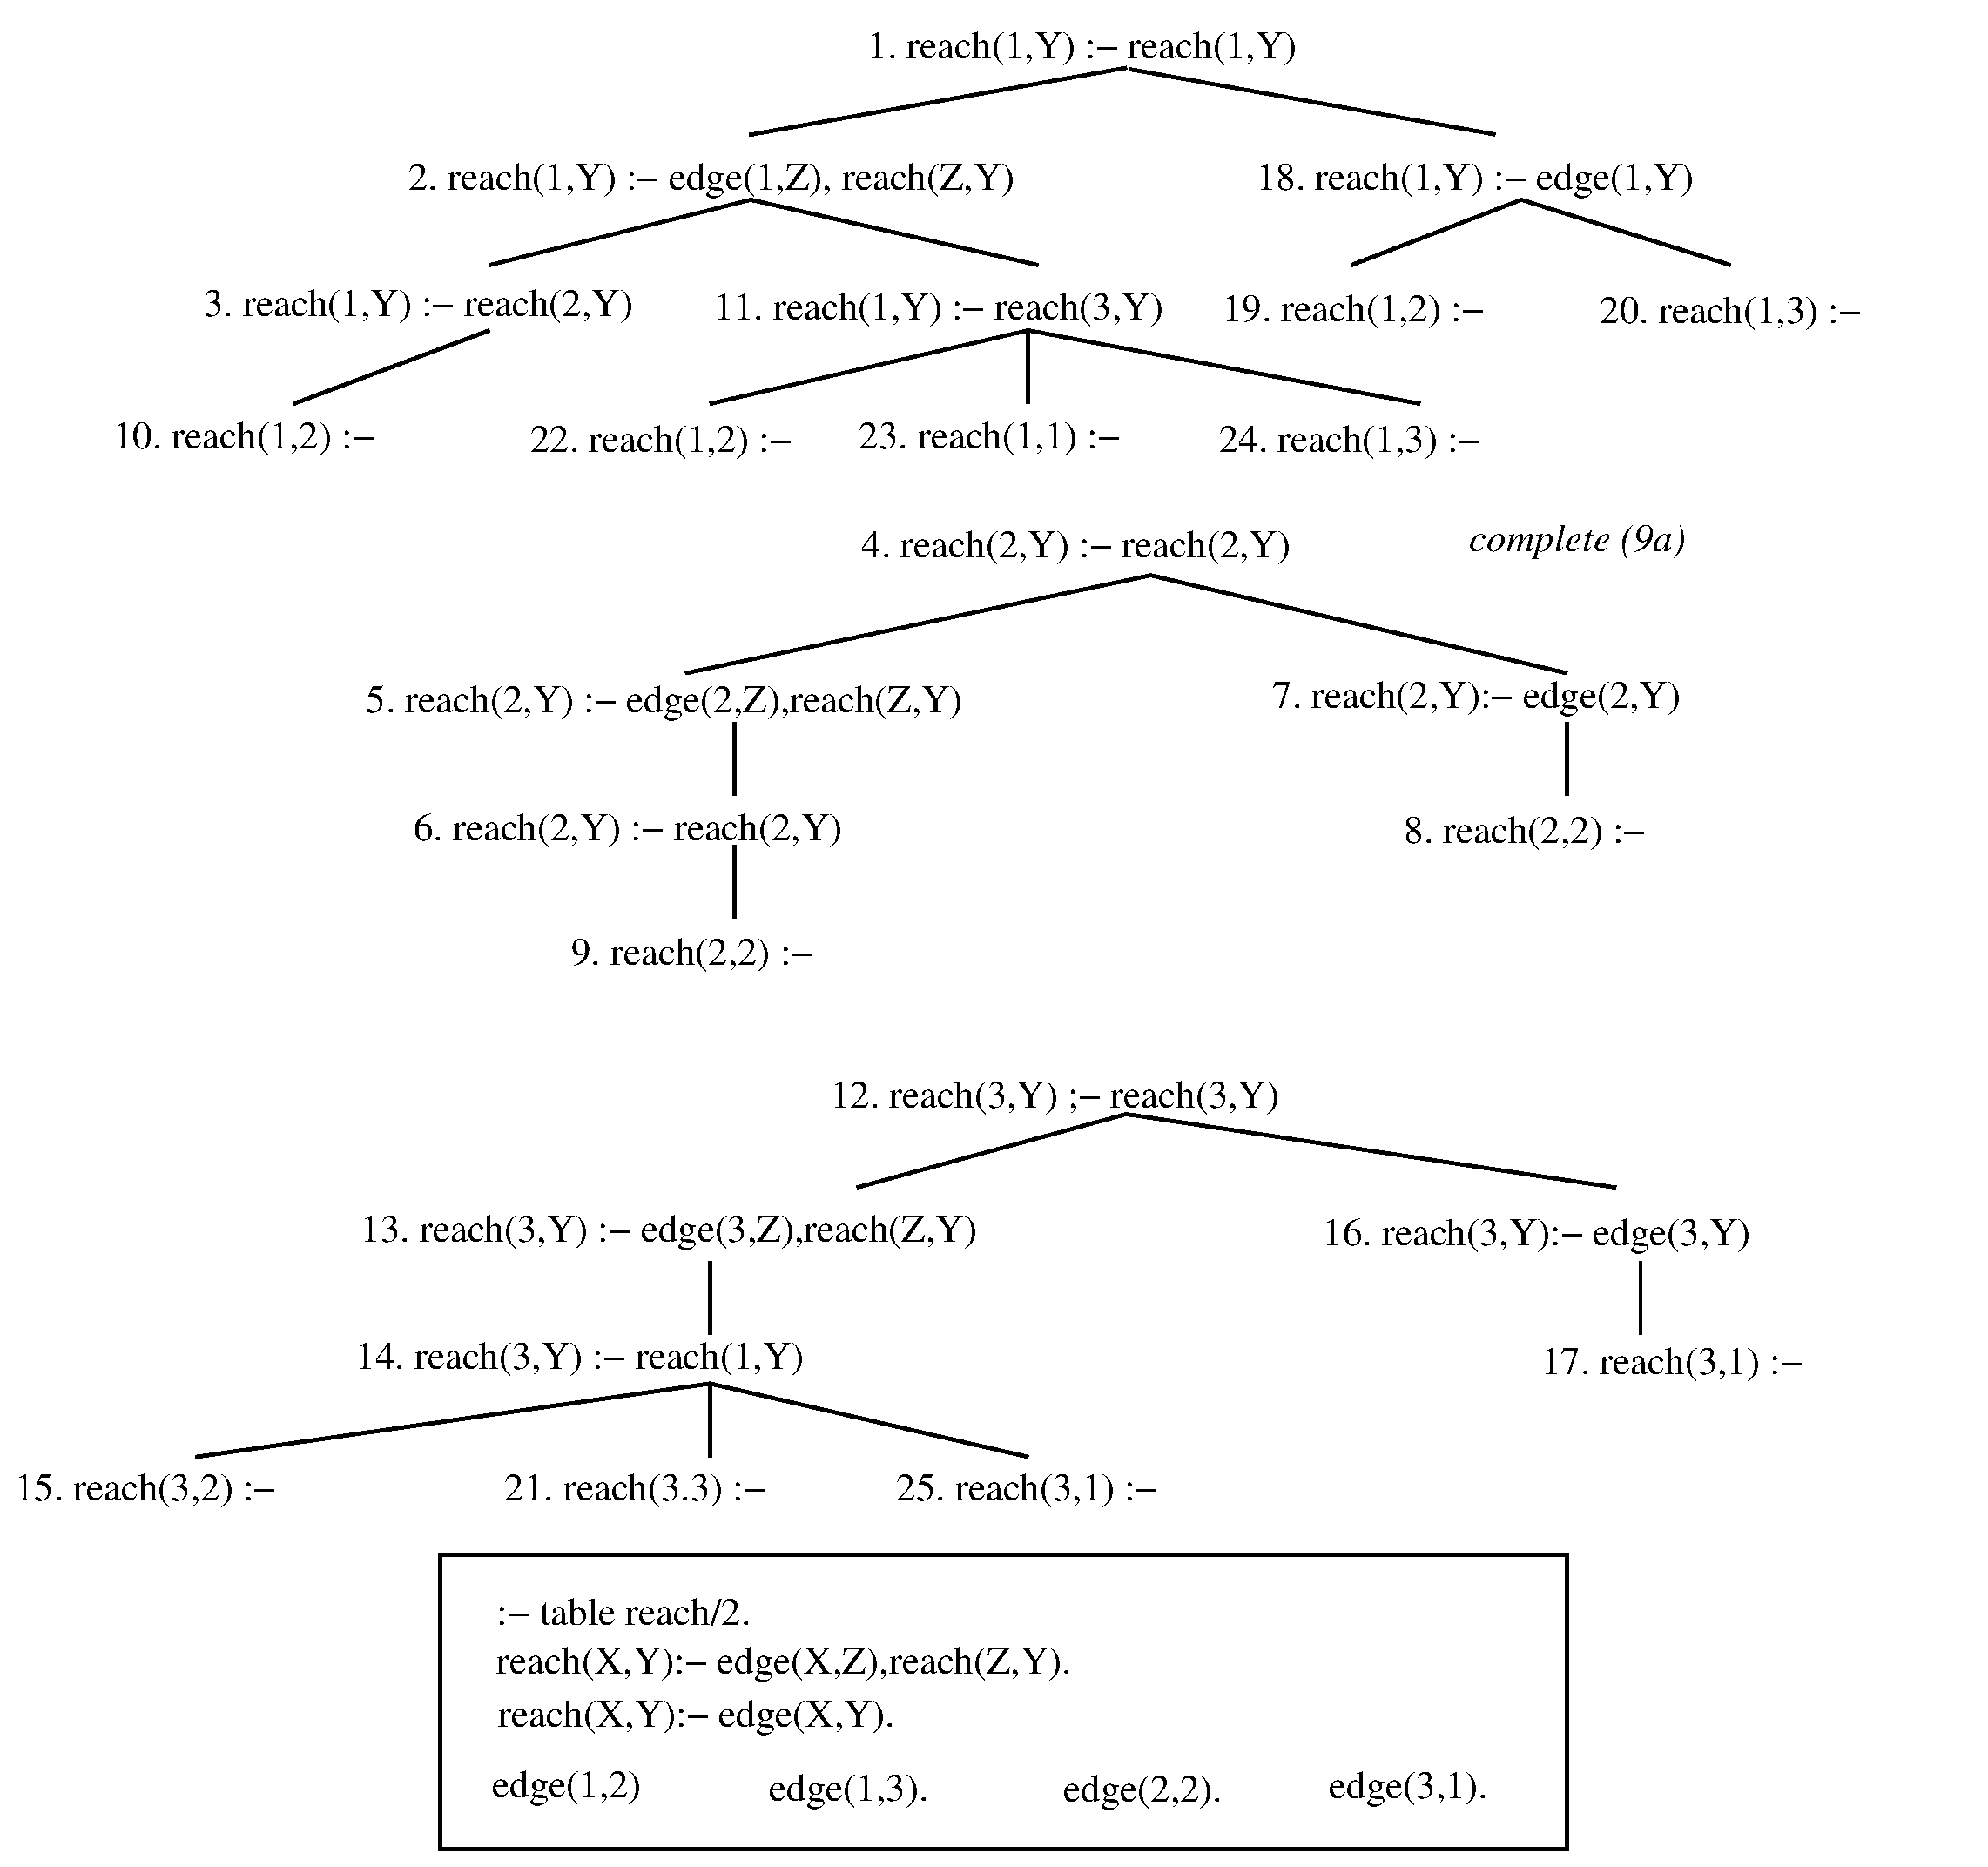
\epsfig{file=slg-forest-local,width=.99\textwidth}}}
\caption{A program $P_{Rrec}$ and SLG forest for (local) evaluation of
  {\tt ?- reach(1,Y)}} \label{fig:local}
\end{figure}
%
Note that the evaluation keeps track of each tabled subgoal $S$ that
it encounters.  Later if $S$ is selected again, resolution will use
answers rather than program clauses; if no answers are available, the
computation will {\em suspend} at that point and the evaluation will
backtrack to try to derive answers using some other computation path.
Once more answers have been derived, the evaluation {\em resumes} the
suspended computation.  Similarly, once the computation has
backtracked through all answers available for $S$ in the current
state, the computation path will suspend, and resume after further
answers are found.  Thus a tabled evaluation is a fixed point
computation for a set of interdependent subgoals.  When it is
etermined that a (perhaps singleton) set of subgoals can produce no
more answers, the subgoals are completed.
\end{example}

%\vspace{0.1in}

The forest logging approach ({\tt \ctrace}) allows one to run a tabled
query and produce a log that can be interpreted as (a partial image
of) an SLG forest.  The log can then used to analyze program
correctness, to optimize performance and so on.  Because \ctrace{}
  produces a log, it superficially resembles the non-interactive trace
  described earlier in this chapter.  However,
\begin{itemize}
\item {\tt trace/1} produces a Prolog-style trace that takes little
  account of tabling.  \ctrace{} structures its output according to
  the forest-of-trees model, and takes little account of program
  clause resolution.

\item \ctrace{} is implemented in C for efficiency, while {\tt
  trace/1} is built on top of XSBs interactive debugger.  Unlike {\tt
  trace/1}, \ctrace{} can therefore to produce logs for very large
  evaluations with little overhead.
\end{itemize}

{\em We stress that the forest logging approch is under development and
  its features are subject to change.}

Currently, \ctrace{} captures the following actions.

\bi
\item {\em A call to a tabled subgoal}~ If a call to a tabled subgoal
  $S_1$ is made from a tree for $S_2$ a Prolog-readable fact of the
  form {\tt tc(S1,S2,Stage,Counter)} is logged, where {\em Counter} is
  the ordinal number of the fact, and {\tt Stage} is
\bi
\item {\tt new} if $S_1$ is a new subgoal
\item {\tt cmp} if $S_1$ is not a new subgoal and has been completed
\item {\tt incmp} if $S_1$ is not a new subgoal but has {\em not} been
  completed \ei
%
  For instance, in the above example, node 3 would be represented as
  {\tt tc(reach(2,Y),reach(1,Y),2)} (the reason for using the counter
  value of 2 rather than 3 is explained below).  If $S_1$ is the first
  tabled subgoal in an evaluation, $S_2$ is the atom {\em null}.

\item {\em Derivation of a new answer}~ When a new answer $A$ is
  derived for subgoal $S$ and added to the table (i.e. $A$ is not
  already an answer for $S$) a fact of the form {\tt na(A,S,Counter)}
  is logged.  In the above example, the answer node 9 would be
  represented as {\tt na([2],reach(2,\_v1),4)} where the first argument
  is a list of substitutions for the variables {\em \_v1,...,\_vn} in
  $S$.

\item {\em Return of an answer to a consuming subgoal}~When an answer
  $A$ is returned to a consuming subgoal $S$ in a tree for $S_T$, a
  fact of the form {\tt ar(A,S,ST,Counter)} is logged.  A log entry is
  made only if the table for $S$ is incomplete (see the explanation
  below).

\item {\em Subgoal completion}
\bi
\item When a set $\cS$ of subgoals is determined to be completely
  evaluated and is completed, a fact of the form {\tt
    cmp(S,SCCNum,Counter)} is logged for each $S \in \cS$.  Here
  $SCCNum$ is simply a number giving an ordinal value that can be used
  to group subgoals into mutually dependent sets of subgoals or SCCs,
  i.e. the {\em SCCNum} of each $S \in \cS$ has the same value, but
  that value is not used for a completion fact of any subgoal not in
  $\cS$.
%
\item When a subgoal $\cS$ is {\em early completed}, i.e. it is
  determined that no more answers for $S$ are possile or are desired a
  fact of the form {\tt cmp(S,ec,Counter)} is logged.  If $S$ belonged
  to a larger mutually dependent set $\cS$ when it was early
  completed, $S$ will also be included in the completion facts for
  $\cS$.
\ei
\item {\em Table Abolishes}
\bi
\item When a tabled subgoal $S$ is abolished, a fact of the form {\tt
  ta(subg(S),Counter)} is logged.
\item When all tables for a predicate $p/n$ are abolished, a fact of
  the form {\tt ta(pred(p/n),Counter)} is logged.
\item When all tables are abolished, a fact of the form {\tt ta(all,Counter)} is logged.
\ei
%
\item {\em Location of errors} Whenever an error is thrown and the
  execution is in a tree for a subgoal $S$, a Prolog-readable fact of
  the form {\tt err(S,Counter)} is logged, where {\em Counter} is the
  ordinal number of the fact.  The primary purpose of this fact is to
  indicate the nearest tabled call that gave rise to an uncaughterror.  \ei

{\tt logforest} does {\em not} contain

\bi
\item Information about the occurrence of program clause resolution
  either when used to produce children of tabled predicates, or when
  it is used to produce children whose nodes have a selected literal
  that is non-tabled.

\item Information about the return of answers from completed tables.
  XSB uses a so-called {\em completed table optimization} which treats
  answer return from completed tables in a manner akin to program
  clause resolution.  
 \ei

\index{attributed variables}
\noindent
The inclusion of the above two features in {\tt logforest} would
significantly slow down execution of XSB.  However, future versions of
{\tt logforest} may include expanded logging features for negation,
for call and answer subsumption and for incremental
tabling~\footnote{Currently, attributes of attributed variables are
  not printed out.}.

\begin{example}
The forest for {\tt reach(1,Y)} in the foregoing example has the log
file as shown in Table~\ref{tab:fview}.

\begin{table}[htbp]
\begin{tabular}{lll}               \\ \hline  
Log File                                     & Forest & Explanation\\ \hline 
tc(reach( 1,\_v0),null,new,0)                & node 1 & \\
                                             & node 2 & created by program clause resol. \\
                                             & node 3 & created by program clause resol. \\
tc(reach( 2,\_v0),reach( 1,\_v0),new,1)      & node 4 & \\
                                             & node 5 & created by program clause resol.\\
                                             & node 6 & created by program clause resol. \\
tc(reach( 2,\_v0),reach( 2,\_v0),incmp,2)    &        & repeated subgoal registered\\
                                             & node 7 & created by program clause resol. \\
                                             & node 8 & created by program clause resol. \\
na([ 2],reach( 2,\_v0),3)                    & node 8 & registered as answer\\
ar([ 2],reach( 2,\_v0),reach( 2,\_v0),4)     & node 9 & created by answer resol.\\
cmp(reach( 2,\_v0),2,5)                      &    9a   & {\tt reach(2,\_v0)} completed \\
                                             & node 10 & created by return from completed table \\
na([ 2],reach( 1,\_v0),6)                    & node 10 & registered as an answer\\
                                             & node 11 & created by program clause resol. \\
tc(reach( 3,\_v0),reach( 1,\_v0),new,7)      & node 12 & \\
                                             & node 13 & created by program clause resol. \\
                                             & node 14 & created by program clause resol. \\
tc(reach( 1,\_v0),reach( 3,\_v0),incmp,8)    & node 14 & repeated subgoal registered \\
ar([ 2],reach( 1,\_v0),reach( 3,\_v0),9)     & node 15 & created by answer resol. \\
na([ 2],reach( 3,\_v0),10)                   & node 15 & registered as an answer \\
                                             & node 16 & created by program clause resol. \\
                                             & node 17 & created by program clause resol. \\
na([ 1],reach( 3,\_v0),11)                   & node 17 & registered as an answer \\
                                             & node 18 & created by program clause resol. \\
                                             & node 19 & created by program clause resol. (repeated answer)\\
                                             & node 20 & created by program clause resol.\\
na([ 3],reach( 1,\_v0),12)                   & node 20 & registered as an answer\\
ar([ 3],reach( 1,\_v0),reach( 3,\_v0),13)    & node 21 & created by answer return\\
na([ 3],reach( 3,\_v0),14)                   & node 21 & registered as an answer\\
ar([ 2],reach( 3,\_v0),reach( 1,\_v0),15)    & node 22 & created by answer resol.\\
ar([ 1],reach( 3,\_v0),reach( 1,\_v0),16)    & node 23 & created by answer resol.\\
na([ 1],reach( 1,\_v0),17)                   & node 23 & registered as an answer \\
ar([ 3],reach( 3,\_v0),reach( 1,\_v0),18)    & node 24 & created by answer resol. \\
ar([ 1],reach( 1,\_v0),reach( 3,\_v0),19)    & node 25 & created by answer resol.v \\
cmp(reach( 1,\_v0),1,20)                     &  & \\
cmp(reach( 3,\_v0),1,21)   & & \\ \hline
\end{tabular}
\caption{Log file for computation in Figure~\ref{fig:local}}\label{tab:fview}
\end{table}
\end{example}

\begin{description}
\ourrepeatmoditem{log\_forest(+Call)}{log\_forest/2}{tables}
\ourmoditem{log\_forest(+Call,+Options)}{log\_forest/2}{tables}
%
These predicates turn on forest logging, call {\tt Call} then turn
logging off.  Currently, the only option is {\tt file(File)}, which
directs the logging to the file {\tt File}.  If {\tt Options} is an
empty list or if {\tt log\_forest/1} is called, the log will be sent
to standard output~\footnote{Future options will be able to turn on
  and off the logging of various types of facts.}.

\index{indexing}
\ourmoditem{load\_forest\_log(+File)}{load\_forest\_log/1}{tables}
%
The log produced by {\tt log\_forest/[1,2]} is a Prolog file that can
be compiled and/or loaded dynamically just as any other Prolog file.
However, for large logs (i.e. those of many megabytes) use of {\tt
  load\_dync/[1,2]} XSB commands can drastically reduce the time
needed to load the file, while use of the proper {\tt index/2}
declarations can greately improve query time.  The simple predicate,
{\tt load\_forest\_log/1} loads a log file and indexes needed arguments.
\end{description}

\index{tracing|)}




%%% Local Variables: 
%%% mode: latex
%%% TeX-master: "manual1"
%%% End: 


\chapter{Definite Clause Grammars} \label{DCGs}
\index{definite clause grammars}\index{grammars!definite clause}
%===============================================================

\section{General Description}
%============================

Definite clause grammars (DCGs) are an extension of context free
grammars that have proven useful for describing natural and formal
languages, and that may be conveniently expressed and executed in
Prolog.  A Definite Clause Grammar rule is executable because it is
just a notational variant of a logic rule that has the following
general form:
\begin{center}
                {\em Head} {\tt \verb|-->|} {\em Body.}
\end{center}
with the declarative interpretation that ``a possible form for {\em
Head} is {\em Body}''. The procedural interpretation of a grammar rule
is that it takes an input sequence of symbols or character codes,
analyses some initial portion of that list, and produces the remaining
portion (possibly enlarged) as output for further analysis.  In XSB,
the exact form of this sequence is determined by whether XSB's {\em
DCG mode} is set to use tabling or not, as will be discussed below.
In either case, the arguments required for the input and output lists
are not written explicitly in the DCG rule, but are added when the
rule is translated (expanded) into an ordinary normal rule during
parsing.  Extra conditions, in the form of explicit Prolog literals or
control constructs such as {\em if-then-elses} ({\tt '->'/2}) or {\em
cuts}\index{cut} (\cut)\index{\texttt{"!/0}}, may be included in the {\em
Body} of the DCG rule and they work exactly as one would expect.

The syntax of DCGs is orthogonal to whether tabling is used for DCGs
or not.  An overview of DCG syntax
 supported by XSB is as follows:
\begin{enumerate}
\item A non-terminal symbol may be any HiLog term other than a variable
      or a number. A variable which appears in the body of a rule is
      equivalent to the appearance of a call to the standard predicate
      {\tt phrase/3} as it is described below.
\item A terminal symbol may be any HiLog term. In order to distinguish 
      terminals from nonterminals, a sequence of one or more terminal
      symbols   $\alpha, \beta, \gamma, \delta, \ldots$
      is written within a grammar rule as a Prolog list 
         {\tt [} $\alpha, \beta, \gamma, \delta, \ldots$ {\tt ]},
      with the empty sequence written as the empty list {\tt [\,]}.
      The list of terminals may contain variables but it has to be a 
      proper list, or else an error message is sent to the standard 
      error stream and the expansion of the grammar rule that contains 
      this list will fail. If the terminal symbols are UTF-8 character
      codes, they can be written (as elsewhere) as strings.
\item Extra conditions, expressed in the form of Prolog predicate calls, 
      can be included in the body (right-hand side) of a grammar rule by 
      enclosing such conditions in curly brackets, {\tt '$\{$'} and
      {\tt '$\}$'}.
      For example, one can write:
      \begin{center}
                {\tt positive\_integer(N) \verb|-->| [N], $\{$integer(N), N > 0$\}$.}
                \footnote{A term like {\tt $\{$foo$\}$} is just a
			  syntactic-sugar for the term {\tt '$\{\}$'(foo)}.}
      \end{center}
\item The left hand side of a DCG rule must consist of a single non-terminal,
      possibly followed by a sequence of terminals (which must be written as
      a {\em unique} Prolog list). Thus in XSB, unlike SB-Prolog 
      version 3.1, Semicontext (formerly called push-back lists) is supported.
\item The right hand side of a DCG rule may contain alternatives (written 
      using the usual Prolog's disjunction operator {\tt ';'} or 
      using the usual BNF disjunction operator {\tt '|'}. 
\item The Prolog control primitives {\em if-then-else} ({\tt '->'/2}),
      {\em nots} ({\tt not/1, fail\_if/1}, \not\ or {\tt tnot/1}) and 
      {\em cut}\index{cut} (\cut)\index{\texttt{"!/0}} may also be included in the 
      right hand side of a DCG rule. These symbols need not be enclosed in 
      curly brackets. 
      \footnote{Readers familiar with Quintus Prolog may notice the difference
                in the treatment of the various kinds of not. For example, in 
                Quintus Prolog a {\tt not/1} that is not enclosed within curly 
                brackets is interpreted as a non-terminal grammar symbol.}
      All other Prolog's control primitives, such as {\tt repeat/0}, must
      be enclosed explicitly within curly brackets if they are not meant
      to be interpreted as non-terminal grammar symbols.
\end{enumerate}
 

\section{Translation of Definite Clause Grammar rules}
%=====================================================

In this section we informally describe the translation of DCG rules
into normal rules in XSB.  Each grammar rule is translated into a
Prolog clause as it is consulted or compiled.  This is accomplished
through a general mechanism of defining the hook predicate {\tt
term\_expansion/2}, \stdrefindex{term\_expansion/2} by means of which
a user can specify any desired transformation to be done as clauses
are read by the reader of XSB's parser.  This DCG term expansion is as
follows:

A DCG rule such as:

\stuff{
\> \> p(X) \dashdashgreater q(X).
}

\noindent
will be translated (expanded) into:

\stuff{
\> \> p(X, Li, Lo) :- \\ 
\> \> \>  q(X, Li, Lo).
}

If there is more than one non-terminal on the right-hand side, as in

\stuff{\> \> p(X, Y) \dashdashgreater q(X), r(X, Y), s(Y).}

\noindent
the corresponding input and output arguments are identified, 
translating into:

\stuff{
\> \> p(X, Y, Li, Lo) :- \\ 
\> \> \> q(X, Li, L1), \\
\> \> \> r(X, Y, L1, L2), \\
\> \> \> s(Y, L2, Lo).
}

Terminals are translated using the predicate {\tt 'C'/3} (See 
section~\ref{DCG_builtins} for its description).  For instance:

\stuff{\> \> p(X) \dashdashgreater [go, to], q(X), [stop].}

\noindent
is translated into:

\stuff{  
\> \> p(X, S0, S) :- \\
\> \> \> 'C'(S0, go, S1), \\
\> \> \> 'C'(S1, to, S2), \\
\> \> \> q(X, S2, S3), \\
\> \> \> 'C'(S3, stop, S).
}

Extra conditions expressed as explicit procedure calls naturally translate
into themselves. For example,

\stuff{
\> \> positive\_number(X) \dashdashgreater \\
\> \> \> [N], $\{$integer(N), N > 0$\}$, \\
\> \> \> fraction(F), $\{$form\_number(N, F, X)$\}$.}

\noindent
translates to:

\stuff{
\> \> positive\_number(X, Li, Lo) :- \\
\> \> \> 'C'(Li, N, L1), \\
\> \> \> integer(N), \\
\> \> \> N > 0, \\
\> \> \> L1 = L2, \\
\> \> \> fraction(F, L2, L3), \\
\> \> \> form\_number(N, F, N), \\
\> \> \> L3 = Lo. \\
}

Similarly, a cut is translated literally.

{\em Semicontext} (or a push-back list, which is a proper list of
terminals on the left-hand side of a DCG rule) translate into a
sequence of {\tt 'C'/3} goals with the first and third arguments
reversed.  For example,

\stuff{\> \> it\_is(X), [is, not] \dashdashgreater [aint].}

\noindent
becomes

\stuff{
\> \> it\_is(X, Li, Lo) :- \\
\> \> \> 'C'(Li, aint, L1), \\
\> \> \> 'C'(Lo, is, L2), \\
\> \> \> 'C'(L2, not, L1).
}

Disjunction has a fairly obvious translation.  For example, the DCG clause:

\stuff{
\> \> expr(E) \dashdashgreater \\
\> \> \> \ \ expr(X), "+", term(Y), $\{$E is X+Y$\}$ \\
\> \> \>   | term(E).
}

\noindent
translates to the Prolog rule:

\stuff{
\> \>expr(E, Li, Lo) :- \\
\> \> \>   ( expr(X, Li, L1), \\
\> \> \> \ \ 'C'(L1, 43, L2), \> \% 0'+ = 43 \\
\> \> \> \ \ term(Y, L2, L3) \\
\> \> \> \ \ E is X+Y, \\
\> \> \> \ \ L3 = Lo \\
\> \> \>   ; term(E, Li, Lo) \\
\> \> \>   ).
}

\subsection{Definite Clause Grammars and Tabling}
%============================================================
\label{sec:dcg_tabling}

Tabling can be used in conjunction with Definite Clause Grammars to get the
effect of a more complete parsing strategy.  When Prolog is used to evaluate
DCG's, the resulting parsing algorithm is {\em ``recursive descent''}.
Recursive descent parsing, while efficiently implementable, is known to
suffer from several deficiencies:  1) its time can be exponential in the size
of the input, and 2) it may not terminate for certain context-free grammars (in
particular, those that are left or doubly recursive).  By appropriate use of
tabling, both of these limitations can be overcome.  With appropriate tabling,
the resulting parsing algorithm is a variant of {\em Earley's algorithm\/} and
of {\em chart parsing algorithms}.

In the simplest cases, one needs only to add the directive {\tt :-
auto\_table} (see Section~\ref{tabling_directives}) to the source file
containing a DCG specification.  This should generate any necessary
table declarations so that infinite loops are avoided (for
context-free grammars).  That is, with a {\tt :- auto\_table}
declaration, left-recursive grammars can be correctly processed.  Of
course, individual {\tt table} directives may also be used, but note
that the arity must be specified as two more than that shown in the
DCG source, to account for the extra arguments added by the expansion.
However, the efficiency of tabling for DCGs depends on the
representation of the input and output sequences used, a topic to
which we now turn.

\index{definite clause grammars!list mode}

Consider the expanded DCG rule from the previous section:

\stuff{ \>
\> p(X, S0, S) :- \\ 
\> \> \> 'C'(S0, go, S1), \\ 
\> \> \> 'C'(S1, to,S2), \\ 
\> \> \> q(X, S2, S3), \\ 
\> \> \> 'C'(S3, stop, S).  } 

In a Prolog system, each input and output variable, such as {\tt S0}
or {\tt S} is bound to a variable or a difference list.  In XSB, this
is called {\em list mode}.  Thus, to parse {\em go to lunch stop} the
phrase would be presented to the DCG rule as a list of tokens {\tt
[go,to,lunch,stop]} via a call to {\tt phrase/3} such as:

\stuff{\> \> phrase(p(X),[go,to,lunch,stop]).}

\noindent
or an explicit call to {\tt p/3}, such as:

\stuff{\> \> p(X,[go,to,lunch,stop|X],X).}

\noindent
Terminal elements of the sequence are consumed (or generated) via the
predicate {\tt 'C'/3} which is defined for Prolog systems as:

\stuff{\> \> 'C'([Token|Rest],Token,Rest).}

While such a definition would also work correctly if a DCG rule were
tabled, the need to copy sequences into or out of a table can lead to
behavior quadratic in the length of the input sequence (See Section
\ref{sec:TablingPitfalls}).  As an alternative, XSB allows a mode of
DCGs that defines {\tt 'C'/3} as a call to a Datalog predicate {\tt
word/3} \stdrefindex{word/3}:

\stuff{\> \> 'C'(Pos,Token,Next\_pos):- word(Pos,Token,Next\_pos).}

\noindent
assuming that each token of the sequence has been asserted as a {\tt
word/3} fact, e.g:

\stuff{
\> \> word(0,go,1). \\
\> \> word(1,to,2). \\
\> \> word(2,lunch,3). \\
\> \> word(3,stop,4).
}

\noindent
The above mode of executing DCGs is called {\em datalog mode}.  
\index{definite clause grammars!datalog mode}

{\tt word/3} facts are asserted via a call to the predicate {\tt
tphrase\_set\_string/1}.  Afterwards, a grammar rule can be called
either directly, or via a call to {\tt tphrase/1}.  To parse the list
{\tt [go,to,lunch,stop]} in datalog mode using the predicate {\tt p/3}
from above, the call

\stuff{\> \> tphrase\_set\_string([go,to,lunch,stop])}

\noindent
would be made, afterwards the sequence could be parsed via the goal:

\stuff{tphrase(p(X)).}

\noindent
or

\stuff{p(X,0,F).}

To summarize, DCGs in list mode have the same syntax as they do in
datalog mode: they just use a different definition of {\tt 'C'/3}.  Of
course tabled and non-tabled DCGs can use either definition of {\tt
'C'/3}.  Indeed, this property is necessary for tabled DCG predicates
to be able to call non-tabled DCG predicates and vice-versa.  At the
same time,tabled DCG rules may execute faster in datalog mode, while
non-tabled DCG rules may execute faster in list mode.

Finally, we note that the mode of DCG parsing is part of XSB's state.
XSB's default mode is to use list mode: the mode is set to datalog
mode via a call to {\tt tphrase\_set\_string/3} and back to list mode
by a call to {\tt phrase/2} or by a call to {\tt reset\_dcg\_mode/0}.

\section{Definite Clause Grammar predicates} \label{DCG_builtins}
%================================================================
The library predicates of XSB that support DCGs are the following:

\begin{description}

\standarditem{phrase(+Phrase, ?List)}{phrase/2}
    This predicate is true iff the list {\tt List} can be parsed as a phrase 
    (i.e. sequence of terminals) of type {\tt Phrase}.  {\tt Phrase} can be 
    any term which would
    be accepted as a nonterminal of the grammar (or in general, it can 
    be any  grammar rule body), and must be instantiated to a
    non-variable term  at the time of the call; otherwise an error
    message is sent to the standard error stream and the predicate fails. 
    This predicate is the usual way to commence execution of grammar rules.

    If {\tt List} is bound to a list of terminals by the time of the call,
    then the goal corresponds to parsing {\tt List} as a phrase of type
    {\tt Phrase}; otherwise if {\tt List} is unbound, then the grammar
    is being used for generation.

\standarditem{tphrase(+Phrase)}{tphrase/1} This predicate
    succeeds if the current database of {\tt word/3} facts can be
    parsed via a call to the term expansion of {\tt +Phrase} whose
    input argument is set to {\tt 0} and whose output argument is set
    to the largest {\tt N} such that {\tt word(\_,\_,N)} is currently
    true.  

    The database of {\tt word/3} facts is assumed to have been
    previously set up via a call to {\tt tphrase\_set\_string/1} (or variant).  If
    the database of {\tt word/3} facts is empty, {\tt tphrase/1} will
    abort.

% TLS: handle error condition better in predicate.

\standarditem{phrase(+Phrase, ?List, ?Rest)}{phrase/3}
    This predicate is true iff the segment between the start of list 
    {\tt List} and the start of list {\tt Rest} can be parsed as a phrase 
    (i.e. sequence of terminals) of type {\tt Phrase} . In other words, if 
    the search for phrase 
    {\tt Phrase} is started at the beginning of list {\tt List}, then 
    {\tt Rest} is what remains unparsed after {\tt Phrase} has been
    found. Again, {\tt Phrase} can be any term which
    would be accepted as a nonterminal of the grammar (or in general, any
    grammar rule body), and must be instantiated to a non-variable term
    at the time of the call; otherwise an error message is sent to the
    standard error stream and the predicate fails.

    Predicate {\tt phrase/3} is the analogue of {\tt call/1} for grammar
    rule bodies, and provides a semantics for variables in the bodies of
    grammar rules.  A variable {\tt X} in a grammar rule body is treated
    as though {\tt phrase(X)} appeared instead, {\tt X} would expand into 
    a call to {\tt phrase(X, L, R)} for some lists {\tt L} and {\tt R}.  

\standarditem{expand\_term(+Term1, ?Term2)}{expand\_term/2} 
%
This predicate is used to transform terms that appear in a Prolog
program before the program is compiled or consulted.  The default
transformation performed by {\tt expand\_term/2} is that when {\tt
  Term1} is a grammar rule, then {\tt Term2} is the corresponding
Prolog clause; otherwise {\tt Term2} is simply {\tt Term1}
unchanged. If {\tt Term1} is not of the proper form, or {\tt Term2}
does not unify with its clausal form, predicate {\tt expand\_term/2}
simply fails.

Users may augment the default transformations by asserting clauses for
the predicate {\tt term\_expansion/2}\stdrefindex{term\_expansion/2}
to {\tt usermod}.  After {\tt term\_expansion(Term\_a,Term\_b)} is
asserted, then if a consulted file contains a clause that unifies with
{\tt Term\_a} the clause will be transformed to {\tt Term\_b} before
further compilation.  ({\tt Term\_b} can be a list of clauses, so 
{\tt term\_expansion} can transform a single clause into a sequence of 
clauses.)
{\tt expand\_term/2} calls user clauses for {\tt
  term\_expansion/2} first; if the expansion succeeds, the transformed
term so obtained is used and the standard grammar rule expansion is
not tried; otherwise, if {\tt Term1} is a grammar rule, then it is
expanded using {\tt dcg/2}; otherwise, {\tt Term1} is used as is.
%Note that predicate {\tt term\_expansion/2} must be defined in the
%XSB's default read-in module ({\tt usermod}) and should be loaded
%there before the compilation begins.

{\bf Example:} 
%
Suppose the following clause is asserted:
%
\begin{verbatim}
?- assert(term_expansion(foo(X),bar(X))).
\end{verbatim}
and that the file {\tt te.P} contains the clause
%
{\tt foo(a)}
%
then the clause will automatically be expanded upon consulting the file:
%
\begin{verbatim}
| ?- [te].
[Compiling /Users/macuser/te]
[te compiled, cpu time used: 0.0170 seconds]
[te loaded]

yes
| ?- bar(X).

X = a

yes
| ?- foo(X).
++Error[XSB/Runtime/P]: [Existence (No procedure usermod : foo / 1 exists)] []
Forward Continuation...
\end{verbatim}

However, {\tt read/[1,2]} does not automatically perform term expansion
%
\begin{verbatim}
| ?- use_module(standard,[expand_term/2]).

yes
| ?- read(X),expand_term(X,Y).
foo(a).

X = foo(a)
Y = bar(a)

yes
\end{verbatim}




\standarditem{'C'(?L1, ?Terminal, ?L2)}{`C'/3}
This predicate generally is of no concern to the user.  Rather it is used 
    in the transformation of terminal symbols in 
    grammar rules and expresses the fact that {\tt L1} is connected 
    to {\tt L2} by the terminal {\tt Terminal}. This predicate is
    needed to avoid problems due to source-level
    transformations in the presence of control primitives such as
    {\em cuts}\index{cut} (\cut)\index{\texttt{"!/0}}, or {\em if-then-elses} 
    ({\tt '->'/2}) and is defined by the single clause:
    \begin{center}
                {\tt 'C'([Token|Tokens], Token, Tokens).}
    \end{center}
    The name 'C' was chosen for this predicate so that another useful
    name might not be preempted.

\standarditem{tphrase\_set\_string(+List)}{tphrase\_set\_string/1}
This predicate 

\begin{enumerate}
\item abolishes all tables;
\item retracts all {\tt word/3} facts from XSB's store; and
\item asserts new {\tt word/3} facts corresponding to {\tt List} as
described in Section \ref{sec:dcg_tabling}.
\end{enumerate}

\noindent
implicitly changing the DCG mode from list to datalog.

\ourmoditem{tphrase\_set\_string\_keeping\_tables(+List)}{tphrase\_set\_string\_keeping\_tables/1}{dcg}
This predicate is the same as {\tt tphrase\_set\_string}, except
it does not abolish any tables.  When using this predicate, the
user is responsible for explicitly abolishing the necessary tables.

\ourmoditem{tphrase\_set\_string\_auto\_abolish(+List)}{tphrase\_set\_string\_auto\_abolish/1}{dcg}
This predicate is the same as {\tt tphrase\_set\_string}, except
it abolishes tables that have been indicated as dcg-supported tables
by a previous call to {\tt set\_dcg\_supported\_table/1}.

\ourmoditem{set\_dcg\_supported\_table(+TabSkel)}{set\_dcg\_supported\_table/1}{dcg}
This predicate is used to indicate to the DCG subsystem that a
particular tabled predicate is part of a DCG grammar, and thus the
contents of its table depends on the string being parsed.  {\tt
TabSkel} must be the skeleton of a tabled predicate.  When {\tt
tphrase\_set\_string\_auto\_abolish/1} is called, all tables that have
been indicated as DCG-supported by a call to this predicate will be
abolished.

\ourmoditem{dcg(+DCG\_Rule, ?Prolog\_Clause)}{dcg/2}{dcg}
    Succeeds iff the DCG rule {\tt DCG\_Rule} translates to the Prolog
    clause {\tt Prolog\_Clause}.  At the time of call, {\tt DCG\_Rule}
    must be bound to a term whose principal functor is {\tt '\verb|-->|'/2}
    or else the predicate fails.  {\tt dcg/2} must be explicitly
    imported from the module {\sf dcg}.

\end{description}


\section{Two differences with other Prologs}\label{sec-dcg-differences}
%===========================================
The DCG expansion provided by XSB is in certain cases different 
from the ones provided by some other Prolog systems (e.g.  Quintus Prolog, 
SICStus Prolog and C-Prolog). The most important of these differences are:
\begin{enumerate}
\item XSB expands a DCG clause in such a way that when a \cut\ is 
      the last goal of the DCG clause, the expanded DCG clause is always 
      {\em steadfast}.

      That is, the DCG clause:

      \stuff{
      \> \> a \dashdashgreater b, ! ; c.
      }

      \noindent
      gets expanded to the clause:

      \stuff{
      \> \> a(A, B) :- b(A, C), !, C = B ;  c(A, B).
      }

      \noindent
      and {\em not\/} to the clause:

      \stuff{
      \> \> a(A, B) :- b(A, B), ! ; c(A, B).
      }

      \noindent
      as in Quintus, SICStus and C Prolog.

      The latter expansion is not just optimized, but it can have a
      {\em different (unintended) meaning} if {\tt a/2} is called with
      its second argument bound.

      However, to obtain the standard expansion provided by the other Prolog
      systems, the user can simply execute:
      
      \stdrefindex{set\_dcg\_style/1}
      \stuff{
        \>\> set\_dcg\_style(standard).
      }
    
      To switch back to the XSB-style DCG's, call
      
      \stuff{
        \>\> set\_dcg\_style(xsb).
      }

\index{definite clause grammars!style}
      This can be done anywhere in the program, or interactively.
      By default, XSB starts with the XSB-style DCG's. To change that,
      start XSB as follows:

      \stuff{
        \> \> xsb -e "set\_dcg\_style(standard)."
        }

      Problems of DCG expansion in the presence of {\em cuts} have been known
      for a long time and almost all Prolog implementations expand a DCG
      clause with a \cut\ in its body in such a way that its expansion is
      steadfast, and has the intended meaning when called with its second
      argument bound.  For that reason almost all Prologs translate the DCG
      clause:

      \stuff{
      \> \> a \dashdashgreater ! ; c.
      }

      \noindent
      to the clause:

      \stuff{
      \> \> a(A, B) :- !, B = A ;  c(A, B).
      }

      \noindent 
      But in our opinion this is just a special case of a \cut\ being
      the last goal in the body of a DCG clause.


      Finally, we note that the choice of DCG style is orthogonal to
      whether the DCG mode is list or datalog.

\item Most of the control predicates of XSB need not be enclosed in
      curly brackets.  A difference with, say Quintus, is that predicates
      {\tt not/1}, {\not}, or {\tt fail\_if/1} do not get expanded when
      encountered in a DCG clause.  That is, the DCG clause:

      \stuff{
      \> \> a \dashdashgreater (true -> X = f(a) ; not(p)).
      }

      \noindent
      gets expanded to the clause:

      \stuff{
      \> \> a(A,B) :- (true(A,C) -> =(X,f(a),C,B) ; not p(A,B))
      }

      and {\em not\/} to the clause:

      \stuff{
      \> \> a(A,B) :- (true(A,C) -> =(X,f(a),C,B) ; not(p,A,B))
      }

      \noindent
      that Quintus Prolog expands to.

      However, note that all non-control but standard predicates (for example 
      {\tt true/0} and {\tt '='/2}) get expanded if they are not enclosed in 
      curly brackets.
\end{enumerate}



%%% Local Variables: 
%%% mode: latex
%%% TeX-master: "manual1"
%%% End: 

\chapter{Exception Handling}\label{chap:exception}
\index{exceptions|(}

We define the term {\em exceptions} as errors in program execution
that are handled by a non-local change in execution state.  Exception
handling in XSB is ISO-compatible, and has been extended to handle
tabled evaluations.  

\section{The Mechanics of Exception Handling}
%
We address the case of non-tabled evaluations before discussing the
extensions for tabling.

\subsection{Exception Handling in Non-Tabled Evaluations}
%
The preferred mechanism for dealing with exceptions in XSB is to use
the predicates {\tt catch/3} and {\tt default\_user\_error\_handler/1}
together together with either one of XSB's error predicates (such as
{\tt misc\_error/1}) or {\tt throw/1}.  These predicates are
ISO-compatible, and their use can give a great deal of control to
exception handling.  At a high level, when an exception is encountered
an error term $T$ is {\em thrown}.  In a Prolog program, throwing an
error term $T$ causes XSB to examine its choice point stack until it
finds a {\em catcher} that unifies with $T$.  This catcher then calls
a {\em handler}.  If no explicit catcher for $T$ exists, a default
handler is invoked, which usually results in an abort, and returns
execution to the top-level of the interpreter, or to the calling C
function.\footnote{Starting in Version 3.5.1, XSB uses the ISO
  compliant {\tt error/2} for error terms, rather than {\tt error/3}
  as in previous versions.}

A handler is set up when {\tt catch(Goal,Catcher,Handler)} is called.
At this point a continuation is saved (i.e. a Prolog choice point),
and {\tt Goal} is called.  If no exceptions are encountered, answers
for {\tt Goal} are obtained as usual.  Within the execution of {\tt
  Goal}, an exception is usually thrown by calling a Prolog predicate
in the {\tt error\_handler} module, or by executing a C-level error
function.  However, if a user-defined error type is desired, the
Prolog predicate {\tt throw/1} can also be called directly.  As
mentioned above, {\tt throw/1} searches for an ancestor of the current
environment called by {\tt catch/3} and whose catcher (second
argument) unifies with {\tt Error}.  If such an ancestor is found,
program execution reverts to the ancestor and all intervening choice
points are removed.  The catcher's {\tt Handler} goal is called and
the exception is thereby handled.  On the other hand, if no ancestor
was called using {\tt catch/3} the system checks whether a clause with
head {\tt default\_user\_error\_handler(Term)} has been asserted, such
that {\tt Term} unifies with {\tt Error}.  If so, this handler is
executed.  If not, XSB's default system error handler in invoked an
error message is output and execution returns to the top level of the
interpreter.

The following, somewhat fanciful example, helps clarify these
concepts~\footnote{Code for this example can be found in {\tt
\$XSBDIR/examples/exceptions.P}.}.  Consider the predicate {\tt
userdiv/2} (Figure~\ref{fig:userdiv}) which is designed to be called
with the first argument instantiated to a number.  A second number is
then read from a console, and the first number is divided by the
second, and unified with the second argument of {\tt userdiv/2}.  By
using {\tt catch/3} and {\tt throw/1} together the various types of
errors can be caught.

%------------------------------------------------------------------------------------------
\begin{figure}[hbtp]
\longline
\begin{small}
\begin{verbatim}
:- import error_writeln/1 from standard.
:- import type_error/4 from error_handler.

userdiv(X,Ans):- 
        catch(userdiv1(X,Ans),mydiv1(Y),handleUserdiv(Y,X)).

userdiv1(X,Ans):- 
        (number(X) -> true; type_error(number,X,userdiv1/2,1)),
        write('Enter a number: '),read(Y),
        (number(Y) -> true ; throw(mydiv1(error1(Y)))),
        (Y < 0 -> throw(mydiv1(error2(Y))); true),
        (Y =:= 0 -> throw(error(zerodivision,userdiv/1,[])); true),
        Ans is X/Y.

handleUserdiv(error1(Y),_X):- 
        error_writeln(['a non-numeric denominator was entered in userdiv/1: ',Y]),fail.
handleUserdiv(error2(Y),_X):- 
        error_writeln(['a negative denominator was entered in userdiv/1: ',Y]),fail.
\end{verbatim}
\end{small}
\caption{The {\tt userdiv/1} program} \label{fig:userdiv}
\longline
\end{figure}
%------------------------------------------------------------------------------------------

The behavior of this program on some representative inputs is shown
below.

\begin{small}
\begin{verbatim}
| ?- userdiv(p(1),F).
++Error[XSB/Runtime/P]: [Type (p(1) in place of number)]  in arg 1 of predicate userdiv1/2
Forward Continuation...
... machine:xsb_backtrace/1
... error_handler:type_error/4
... standard:call/1
... x_interp:_$call/1
... x_interp:call_query/1
... standard:call/1
... standard:catch/3
... x_interp:interpreter/0
... loader:ll_code_call/3
... standard:call/1
... standard:catch/3

no
| ?- userdiv(3,F).
Enter a number: foo.
a non-numeric denominator was entered in userdiv/1: foo

no
|| ?- userdiv(3,F).
Enter a number: -1.
a negative denominator was entered in userdiv/1: -1

no
| ?- userdiv(3,Y).
Enter a number: 2.

Y = 1.5000

yes
\end{verbatim}
\end{small}

\noindent
Note, however the following behavior.

\begin{small}
\begin{verbatim}
| ?- userdiv(3,F).
Enter a number: 0.
++Error[XSB/Runtime/P] uncaught exception: error(zerodivision,userdiv / 1)
Aborting...
\end{verbatim}
\end{small}

\noindent
By examining the program above, it can be seen that if {\tt p(1)} is
entered, the predicate {\tt type\_error/3} is called.  {\tt
  type\_error/3} is an XSB mechanism to throw a type error from
Prolog.  Error terms thrown by system predicates such as {\tt
  type\_error/3} are in XSB's {\em standard error format}, which is
ISO-compatable and which may encode useful information.  For instance,
the type error thrown in the above example is known to XSB's default
system error handler which prints out a message along with a {\em
  backtrace} that indicates the calling context in which the error
arose (this behavior can be controlled: see
Section~\ref{sec:backtrace}).  Alternately, in the second case, when
{\tt -1} is entered, the (non-standard) error term {\tt
  mydiv1(error2(-1))} is thrown, which is caught within {\tt
  userdiv/2} and handled by {\tt handleUserdiv/2}.  Finally, when {\tt
  0} is entered for the denominator, an error term of the form {\tt
  error(zerodivision,userdiv/1)} is thrown, and that this term does
not unify with the second argument of the {\tt catch/3} literal in the
body of {\tt userdiv/1}, or with any error in standard format.  The
error is instead caught by XSB's default system error handler which
prints an uncaught exception message and aborts to the top level of
the interpreter.

XSB has two default system error handlers: one used when XSB is called
as a stand-alone process, and another when XSB is embedded in a
process.  Each recognizes certain error formats (see Section
\ref{sec:iso-errors}), and handles the rest as uncaught exceptions.
However, there may be times when an application requires special
default handling: perhaps the application calls XSB from through a
socket, so that aborts are not practical.  As another example, perhaps
XSB is being called from a graphical user interface via
Interprolog~\cite{Cale01} or some other interface, so that in addition
to a special abort handling, one would like to display an error
window.  In these cases it is convenient to make use of the dynamic
predicate {\tt default\_user\_error\_handler/1}.  {\tt
  default\_user\_error\_handler/1} is called immediately before the
default system error handler, and after it is ascertained that no
catcher for an error term is available via a {\tt catch/3} ancestor.
It is important to note that the system error handlers catch errors
only in the main thread, and do not affect errors thrown by goals
executed by {\tt thread\_create/[2,3]}.  Error terms thrown by goals
executed by non-detached threads are stored internally, and can be
obtained by {\tt thread\_join/2}.  Error terms thrown by detached
threads are lost when the thread exits, so that any error handling for
a detached thread should be performed within the thread itself.  See
Chapter~\ref{chap:threads} for further information.

Accordingly, suppose the following clause is asserted into {\tt
usermod}:
%
\begin{small}
\begin{verbatim}
?- assert((default_user_error_handler(error(zerodivision,Pred)):- 
        error_writeln(['Aborting: division by 0 in: ',Pred]))).
\end{verbatim}
\end{small}
%
The behavior will now be
\begin{small}
\begin{verbatim}
| ?- userdiv(4,F).
Enter a number: 0.
Aborting: division by 0 in: userdiv / 1
\end{verbatim}
\end{small}
The actions of {\tt catch/3} and {\tt throw/1} resemble that of the
Prolog cut in that they remove choice points that lie between a call
to {\tt throw/1} and the matching {\tt catch/3} that serves as its
ancestor. 

% However, if this process encounters a choice point for an
%incomplete table, execution is aborted to the top user level.

The predicate {\tt call\_cleanup/2}
(cf. Section~\ref{meta_predicates}) can be used with {\tt catch/3},
since the goal {\tt call\_cleanup(Goal,Cleanup)} executes {\tt
  Cleanup} whenever computation of {\tt Goal} is completed, whether
because {\tt Goal} has thrown an exception, has failed, or has
succeeded with its last answer.  {\tt call\_cleanup/2} can thus be
used to release resources created by {\tt Goal} (such as streams,
mutexes, database cursors, etc.).  However, if {\tt Goal} throws an
exception, {\tt call\_cleanup/2} will re-throw the exception after
executing cleanup.

\index{tabling!and exceptions}
\index{strongly connected components (SCCs)}
\subsection{Exception Handling in Tabled Evaluation} \label{sec:exceptions-w-tables}
%
The exception handling as previously described requires extensions in
order to work well with tabled predicates.  First, if an {\em
  unhandled} exception is thrown duing evaluation of a tabled subgoal
$S$ and $S$ is not completed, the table for $S$ is not meaningful and
should be removed.  (Tables that have been completed are not affected
by exceptions.)  Accordingly, the user will sometimes see the message:
%
\begin{verbatim}
   Removing incomplete tables...
\end{verbatim}
%
written to standard feedback.  But what about exceptions that are {\em
  caught} during the computation of $S$?

The proper action to take in such a case is complicated by the
scheduling mechanism of tabling which, as discussed in
Chapter~\ref{chap:TablingOverview}, is more complex than in Prolog.
Rather than a simple depth-first search, as in Prolog, tabled
evaluations effectively perform a series of fixed-point computations
for various sets of mutually dependent subgoals, which are termed {\em
  SCCs}~\footnote{This term is used since sets of mutually dependent
  subgoals are formally modelled as (approximate) {\em Strongly
    Connected Components} within a dependency graph.}.  In fact, a
tabled evaluation can be seen as a tree of SCCs (in batched
evaluation) or a chain of SCCs (in local evaluation).  In a tabled
evalution XSB's throw mechanism searches for the nearest catcher $C$
among its ancestors
%
\begin{itemize}
\item whose first argument unifies with the thrown error; and
\item where $C$ is between SCCs: that is where the set of subgoals
  that depend on $C$ is disjoint from the set of subgoals upon which
  $C$ depends.  We term this the {\em SCC restriction} for exception
  handling.
\end{itemize}
%

This behavior can be best understood by an example.  Consider the
query {\tt a(X)} to the program in Figure~\ref{fig:tab_except} which
has the following output:
%
%-------------------------------------------------------------------------------
\begin{figure}[bhtp]
\longline
\begin{small}
\begin{verbatim}
:- table a/1, b/1, c/1,d/1.
a(X):- writeln(a_calling_b),b(X).

b(X):- writeln(b_calling_a),a(X).
b(X):- writeln(b_calling_c),catch(c(X),_,(writeln(handled_1),fail)).

c(X):- writeln(c_calling_d),d(X).
c(X):- writeln(c_aborting),abort.
d(X):- writeln(d_calling_c),catch(c(X),_,(writeln(handled_2),fail)).
\end{verbatim}
\end{small}
\caption{A program to illustrate exception handling in tabled evaluations} \label{fig:tab_except}
\longline
\end{figure}
%------------------------------------------------------------------------------

\begin{small}
\begin{verbatim}
   | ?- a(X).
   a_calling_b
   b_calling_a
   b_calling_c
   c_calling_d
   d_calling_c
   c_aborting
   Removing incomplete tables...
   handled_1
\end{verbatim}
\end{small}
%
Note that there are 2 SCCs, $\{a(X),b(X)\}$ and $\{c(X),d(X)\}$.  When
the {\tt abort} is called in the body of {\tt c(X)} the catch in the
body of {\tt d(X)} is its nearest ancestor; however this catch is
skipped over, and the catch in the body of {\tt b(X)} takes effect.
This catch is between the SCCs -- the first SCC depends on it, but the
second doesn't.
%
Due to the SCC restriction, the actual behavior of exception handling
with tabling is thus somewhat less intuitive than in Prolog.  If this
restriction were lifted, there would be no guarantee that there
existed a unique catch that was the closest ancestor of an exception.

While the above mechanism offers a great deal of flexibility, for many
cases the best approach to exception handling is to keep it simple.
%
\begin{enumerate}
\item Use catches when there will be no tabled subgoal between an
  exception and its catcher.  For instance, sometimes it may be
  annoying to have {\tt atom\_codes/2} throw an exception rather than
  failing, if given an integer in its first argument.  This can be
  addressed by the predicate
%
\begin{verbatim}
my_atom_codes(X,Y):- 
   catch(atom_codes(1,B),error(type_error(A,B),C,D),writeln(E)).
\end{verbatim}
%
which, for a type error, does not interact with tabling in any way.  
%
\item Similarly, if only subgoals to {\em completed} tables occur
  between an exception and its catcher, exception handling behaves
  just as in case 1).
%
\item Otherwise, abort the entire tabled computation and handle it
  from there.  (Unless you really know what you're doing!)
\end{enumerate}
%

\index{Prolog flags!{\tt exception\_pre\_action}}
\index{strongly connected components (SCCs)}
\index{\texttt{print\_incomplete\_tables/0}}
\subsubsection{Obtaining Information about a Tabled Computation after an Exception is Thrown}
%
XSB backtraces (Section~\ref{sec:backtrace}) provide information about
the context in which error is thrown, but in a tabled computation
additional information is available.  If the Prolog flag {\tt
  exception\_pre\_action} is set to {\tt print\_incomplete\_tables}
(its default setting is {\tt none}), then when an exception is thrown,
incomplete tables and their SCC information at the time an exception
is thrown are printed to a file via {\tt print\_incomplete\_tables/1}.
The file may be obtained through the predicate {\tt
  get\_scc\_dumpfile/1} in the module {\tt tables}.  No file is
generated unless the exception is thrown over at least one incomplete
table.

\section{XSB's Standard Format for Errors} \label{sec:iso-errors}
\index{ISO!errors}

All exceptions that occur during the execution of an XSB program can
be caught.  However, by structuring error terms in a consistent
manner, different classes of errors can be handled much more easily by
handlers, both system- and user-defined.  This philosophy partly
underlies the ISO Standard for defining classes of Prolog errors
\cite{ISO-Prolog}.  While the ISO standard defines various types of
errors and how they should arise during execution of ISO Prolog
predicates, it only partially defines the actual error terms a system
should use.  The ISO format can be represented as:

\begin{center}
{\tt error(Tag,Context), }
\end{center}

\noindent
where {\tt Tag} is specific to each class of error, while {\tt
  Context} is implementation-dependent.\footnote{If a program catches
  errors itself, {\tt error/2} may need to be imported from {\tt
    error\_handler}.}

\subsection{Error Tags}

In XSB, the ISO-compliant values for {\tt Tag} are given below.

\begin{description}
\item[{\tt domain\_error(Valid\_type,Culprit)}] is the tag for an ISO
  domain error, where {\tt Valid\_type} is the domain expected and
  {\tt Culprit} is the term observed.  Various ISO predicates may have
  specific domains for input values; and in addition unlike types,
  domains can be user-defined.
%
\item[{\tt evaluation\_error(Flag)}] is the tag for an ISO evaluation
  error (e.g. overflow or underflow), and {\tt Flag} is the type of
  evaluation error encountered (e.g., {\tt undefined}, if an
  arithmetic function is undefined for a given input).
%
\item[{\tt existence\_error(Type,Culprit)}] is the tag for an ISO
  existence error, where {\tt Type} is the type of a resource (e.g., a
  predicate, stream, attribute handler, etc.) and {\tt Culprit} is the
  term observed.
%
\item[{\tt instantiation\_error}] is the tag for an ISO instantiation
  error.
%
\item[{\tt permission\_error(Op,Obj\_type,Culprit)}] is the tag for an ISO
  permission error, when an operation {\tt Op} was applied to an
  object of type {\tt Obj\_type}, but {\tt Culprit} was observed.
%
\item[{\tt representation\_error(Flag)}] is the tag for an ISO
  representation error (e.g., the maximum arity of a predicate has
  been exceeded), and {\tt Flag} is the type of representation error
  encountered.
%
\item[{\tt resource\_error(Flag)}] is the tag for an ISO resource error
  (e.g. allowed memory has been used, or too many files have been
  opened), and {\tt Flag} is the type of resource error encountered.
%
\item {\tt syntax\_error} and {\tt syntax\_error(Culprit)} are alternate
  tags for an ISO syntax error, where {\tt Culprit} denotes a
  syntactically-incorrect sequence of tokens.
%
\item {\tt system\_error(Flag)} is the tag for an ISO system
  error, and {\tt Flag} is the type of system error encountered.
%
\item {\tt type\_error(Valid\_type,Culprit)} is the tag for an
  ISO type error, where {\tt Valid\_type} is the type expected and
  {\tt Culprit} is the term observed.  As opposed to domain errors,
  type errors should be used for checks of Prolog types only
  (i.e. integers, floats, atoms, etc.)
%
\end{description}

\noindent
In addition, XSB also makes use of two other classes of errors.
%
\begin{description}
\item[{\tt table\_error}] and {\tt type\_error(Subtype)} are the tags for an
  error arising when using XSB's tabling mechanism, when the condition
  giving rise to the error does npt easily fit under one of the above
  classes.
%
\item[{\tt misc\_error}] is the tag for an error that is not
  otherwise classified.
%
\item[{\tt error(thread\_cancel,Id)}] is the format of an error ball for a
  thread that has been cancelled by XSB thread {\tt Id} (See
  Chapter~\ref{chap:threads} for details on thread cancellation.)
%
\end{description}

In \version{} of XSB, errors for ISO predicates usually, but not not
always ISO-compliant, although the number of such non-compliances will
reduce over time. First, when XSB determines it is out of available
system memory, recovering from such an error may be difficult at best.
Accordingly the computation is aborted in the sequential engine, or
XSB exits in the multi-threaded engine~\footnote{This does not include
  overflowaing a memory limit specified by the flag {\tt
    max\_memory}.}.  Second, errors in XSB code sometimes arise as
miscellaneous errors rather than as a designated ISO-error type.

\subsection{XSB-Specific Information in Error Terms}

XSB also encodes other information in error terms, which may vary with
the error thrown, the form in which XSB was compiled, and the version
of XSB.  In addition, the specifics of how the information is
represented may vary, so that this information should always be
represented through the access methods described in this and the next
section.

\begin{description}

\item[{\tt Message}] describes the error in human-readable format.
  Messages are present in all of XSB's system errors, and can be
  obtained through {\tt xsb\_error\_get\_message/2}.

\item[{\tt Goal}] is an atom representing the tabled goal that is
  closest to the environment of the thrown error.  It is present in n
  some, but not all error terms thrown by XSB and can be obtained
  through {\tt xsb\_error\_get\_goal/2}.

\item[{\tt Thread Id}] is an atom {\tt 'th <tid>'} indicating the id
  of the thread that threw the error.  Thread Id information is only
  present when using the multi-threaded version of XSB, and even in
  that version is not present in all error terms.  The predicate {\tt
    xsb\_error\_get\_tid/2} can be used to obtain this information if
  present.

\item[{\tt Backtrace}] represents the stack of the forward
  continuations in the execution stack at the time the error was
  thrown.  Backtraces are present by default in all XSB system error
  terms, and are described in Section~\ref{sec:backtrace}.  They may be
  obtained from an error term using the predicate {\tt
    xsb\_error\_get\_backtrace/2}.

\end{description}

%---------------------------------------------------------------------------------------
\section{Predicates to Throw and Handle Errors}
\label{sec:errorpredicates}

\subsection{Predicates to Throw Errors}

XSB provides a variety of predicates that throw errors~\footnote{C
  functions for throwing terms and ISO-style errors are described in
  Volume 2, Chapter 3 {\em Foreign Language Interface}.}. In general,
we recommend the use of predicates such as {\tt domain\_error/4} over
the direct use of {\tt throw/1} when possible.
%
\begin{description}
\isoitem{throw(+ErrorTerm)}{throw/1}
%
Throws the error {\tt ErrorTerm}.  Execution traverses up the choice
point stack until a goal of the form {\tt catch(Goal,Term,Handler)} is
found such that {\tt Term} unifies with {\tt ErrorTerm}.  In this
case, {\tt Handler} is called.  If no catcher is found in the main
thread, the system looks for a clause of {\tt
  default\_user\_error\_handler(Term)} such that {\tt Term} unifies
with {\tt ErrorTerm} --- if no such clause is found the default system
error handler is called.  In a non-main joinable thread, the error
term is stored internally and the thread exits; in a detached thread,
the thread exits with no action taken.  {\tt throw/1} is most useful
in conjunction with specialized handlers for new types of errors not
already supported in XSB.  
%
\ourmoditem{domain\_error(+Valid\_type,-Culprit,+Predicate,+Arg)}{domain\_error/4}{error\_handler}
%
Throws a domain error.  Using the default system error handler (with
the Prolog flag {\tt backtrace\_on\_error} set to off) an example is
{\small
\begin{verbatim}
domain_error(posInt,-1,checkPosInt/3,3).
++Error[XSB/Runtime/P]: [Domain (-1 not in domain posInt)] in arg 3 of predicate 
checkPosInt/3
\end{verbatim} }
%
\ourmoditem{evaluation\_error(+Flag,+Predicate,+Arg)}{evaluation\_error/3}{error\_handler}
%
Throws an evaluation error.  Using the default system error handler
(with the Prolog flag {\tt backtrace\_on\_error} set to off) an
example is {\small
\begin{verbatim}
evaluation_error(zero_divisor,unidiv/1,2).
++Error[XSB/Runtime/P]: [Evaluation (zero_divisor)] in arg 2 of predicate unidiv/2
\end{verbatim} }
%
\ourmoditem{existence\_error(+Object\_type,?Culprit,+Predicate,+Arg)}{existence\_error/4}{error\_handler}
%
Throws an existence error.  Using the default system error handler
(with the Prolog flag {\tt backtrace\_on\_error} set to off) an
example is {\small
\begin{verbatim}
existence_error(file,'myfile.P','load_intensional_rules/2',2).
++Error[XSB/Runtime/P]: [Existence (No file myfile.P exists)]  in arg 2 of predicate 
load_intensional_rules/2
\end{verbatim}
}
%
\ourmoditem{instantiation\_error(+Predicate,+Arg,+State)}{instantiation\_error/4}{error\_handler}
%
Throws an instantiation error.  Using the default system error
handler, an example (with the Prolog flag {\tt backtrace\_on\_error}
set to off) is {\small
\begin{verbatim}
?- instantiation_error(foo/1,1,nonvar).
++Error[XSB/Runtime/P]: [Instantiation]  in arg 1 of predicate foo/1: must be nonvar
\end{verbatim}
}
%
\ourmoditem{permission\_error(+Op,+Obj\_type,?Culprit,+Predicate)}{permission\_error/4}{error\_handler}
%
Throws a permission error.  Using the default system error handler, an
example (with the Prolog flag {\tt backtrace\_on\_error} set to off)
is {\small
\begin{verbatim}
| ?- permission_error(write,file,'myfile.P',foo/1).
++Error[XSB/Runtime/P]: [Permission (Operation) write on file: myfile.P]  in foo/1
\end{verbatim}
}
%
\ourmoditem{representation\_error(+Flag,+Predicate,+Arg)}{representation\_error/3}{error\_handler}
% 
Throws a representation error.  Using the default system error handler, an
example (with the Prolog flag {\tt backtrace\_on\_error} set to off) is {\small
\begin{verbatim}
representation_error(max_arity,assert/1,1).
++Error[XSB/Runtime/P]: [Representation (max_arity)] in arg 1 of predicate assert/1
\end{verbatim} }
%
\ourmoditem{resource\_error(+Flag,+Predicate)}{resource\_error/3}{error\_handler}
%
Throws a resource error.  Using the default system error handler
(with the Prolog flag {\tt backtrace\_on\_error} set to off) and example is {\small
\begin{verbatim}
resource_error(open_files,open/3)
++Error[XSB/Runtime/P]: [Resource (open_files)] in predicate open/3
\end{verbatim} }
%
\ourmoditem{type\_error(+Valid\_type,-Culprit,+Predicate,+Arg)}{type\_error/4}{error\_handler}
%
Throws a type error.  Using the default system error handler, an
example (with the Prolog flag {\tt backtrace\_on\_error} set to off)
is {\small
\begin{verbatim}
| ?- type_error(atom,f(1),foo/1,1).
++Error[XSB/Runtime/P]: [Type (f(1) in place of atom)]  in arg 1 of predicate foo/1
\end{verbatim}
}
%
\ourmoditem{misc\_error(+Message)}{misc\_error/1}{error\_handler}
%
Throws a miscellaneous error that will be caught by the default system
handler.  For good programming practice miscellaneous errors should
only be thrown when the cases above are not applicable, and the type
of error is not of interest for structured error handling.  Such
situations occur can occur for instance in debugging, during program
development. or for other reasons.  Note that this {\tt misc\_error/2}
replaces the obsolescent XSB predicates {\tt abort/1} and {\tt
  abort/2}.
%
\end{description}
%
% \ouritem{abort}\index{\texttt{abort/0}}
% Abandons the current execution and returns to the top level.  This
%     predicate should normally normally be used: 
% \begin{itemize} 
%\item when a non-ISO exception has occurred and the user wishes to
%abort the computation to the top-level of the interpreter.  
%
%\item {\em and} the type of the error is not of interest for
%structuring error handling.
%\end{itemize}
%
%Such situations occur can occur for instance in debugging, during
%program development, or in small-special purpose programs.
%
% \ouritem{abort(+Message)}\index{\texttt{abort/1}} \index{\texttt{STDERR}}
%    Acts as {\tt abort/0} but sents {\tt Message} to {\tt STDERR}
%    before aborting.

\subsection{Predicates used in Handling Errors}~\label{sec:catch}
%
For best results, output for handling errors should be sent to XSB's
standard error stream using the alias {\tt user\_error} or one of the
predicates described below.

\begin{description}
\isoitem{catch(?Goal,?CatchTerm,+Handler)}{catch/3}
%
Calls {\tt Goal}, and sets up information so that future throws will
be able to access {\tt CatchTerm} under the mechanism mentioned
above. {\tt catch/3} does not attempt to clean up system level
resources with the exception of incomplete tables, which are abolished
as discussed in Section~\ref{sec:exceptions-w-tables}.  However, it is
left up to the handler to close any open files, reset current input
and output, and so on \footnote{cf. the default system error handler,
  which performs these functions, if needed.}.
%
\standarditem{default\_user\_error\_handler(?CatchTerm)}{default\_user\_error\_handler/1}
%
Handles any error terms that unify with {\tt CatchTerm} that are not
caught by invocations of {\tt catch/3}.  This predicate closes open
tables and release mutexes held by the calling thread, but does not
attempt to clean up other system level resources, which is left to the
handler.
%

\index{streams!STDERR}
\ourrepeatmoditem{error\_write(?Message)}{error\_write/1}{standard}
\ourmoditem{error\_writeln(?Message)}{error\_writeln/1}{standard}
%
Utility routines for user-defined error catching.  These predicates
output {\tt Message} to XSB's {\tt STDERR} stream, rather than to
XSB's {\tt STDOUT} stream, as does {\tt write/1} and {\tt writeln/1}.
In addition, if {\tt Message} is a comma list, the elements in the
comma list are output as if they were concatenated together.  Each of
these predicates must be implicitly from the module {\tt standard}.

\ourmoditem{xsb\_error\_get\_message(Error,Message)}{\tt
  xsb\_error\_get\_message/2}{error\_handler} 
%
Obtains the message associated with an error in XSB's standard format.
All errors in standard format have messages.

\ourmoditem{xsb\_error\_get\_goal(Error,?GoalAtom}{xsb\_error\_get\_goal/2}{error\_handler}
%
Obtains the goal (represented as an atom), if any, from an error term
that is in XSB's standard format.  If the error term has no goal, the
predicate fails.

\ourmoditem{xsb\_error\_get\_tid(Error,?Tid)}{xsb\_error\_get\_tid/2}{error\_handler} 
%
Obtains the atom {\tt 'th <tid>'} indicating the id of the thread that
threw the error.  Thread Id information is only present when using the
multi-threaded version of XSB, and even in that version is not present
in all error terms.  

\ourmoditem{xsb\_error\_get\_backtrace(+Error,-Backtrace)}
{xsb\_error\_get\_backtrace/2}{error\_handler} 
%
Obtains the backtrace --- the stack of the forward continuations in
the execution stack at the time the error was thrown.  Backtraces are
present by default in all XSB system error terms, and are described in
Section~\ref{sec:backtrace}.

%\ourmoditem{close\_open\_tables}{close\_open\_tables/0}{machine}
%
%Removes table data structures for all incomplete tables, but does not
%affect any complete tables.  In \version{} this predicate should only
%be used to handle exceptions in {\tt default\_user\_error\_handler/1}.
%In addition, for the multi-threaded engine, this predicate unlocks any
%system mutexes held by the thread calling this predicate.

\end{description}

%----------------------------------------------------------------------------
\section{Convenience Predicates}

The following convenience predicates are provided to make a commonly
used check and to throw an ISO error if the check is not satisfied;
some are written directly in C for speed.  All these predicates must
be imported from the module {\tt error\_handler}, which also contains
provides a few other specialized checks.

\begin{description}
\ourmoditem{check\_acyclic(?Term,+Predicate,+Arg)}{check\_acyclic/3}{error\_handler}
%
Checks that {\tt Term} is acyclic.  If so, the predicate succeeds;
if not it throws a miscellaneous error.

\ourmoditem{check\_atom(?Term,+Predicate,+Arg)}{check\_atom/3}{error\_handler}
%
Checks that {\tt Term} is an atom.  If so, the predicate succeeds;
if not it throws a type error.

\ourmoditem{check\_callable(?Term,+Predicate,+Arg)}{check\_callable/3}{error\_handler}
%
Checks that {\tt Term} is callable.  If so, the predicate succeeds; if
not it throws a type error.

\ourmoditem{check\_ground(?Term,+Predicate,+Arg)}{check\_ground/3}{error\_handler}
%
Checks that {\tt Term} is ground.  If so, the predicate succeeds;
if not it throws an instantiation error.

\ourmoditem{check\_integer(?Term,+Predicate,+Arg)}{check\_integern/3}{error\_handler}
%
Checks that {\tt Term} is an integer.  If so, the predicate succeeds;
if not it throws a type error.

\ourmoditem{check\_nonvar(?Term,+Predicate,+Arg)}{check\_nonvar/3}{error\_handler}
%
Checks that {\tt Term} is not a variable.  If not, the predicate succeeds;
if {\tt Term} is a variable,  it throws an instantiation error.

\ourmoditem{check\_nonvar\_list(?Term,+Predicate,+Arg)}{check\_nonvar\_list/3}{error\_handler}
%
Checks that {\tt Term} is a list, each of whose elements is ground.
If so, the predicate succeeds; if not it throws an instantiation
error.
	    
\ourmoditem{check\_one\_thread(+Operation,+Object\_Type,+Predicate)}{check\_one\_thread/3}{error\_handler}
%
In the multi-threaded engine, {\tt check\_one\_thread/3} checks that
there is only one active thread: if not, a miscellaneous error is
thrown indicating that {\tt Operation} is not permitted on {\tt
  ObjectType} as called by {\tt Predicate}, when more than one thread
is active.  This check provides a convenient way to allow inclusion of
certain operations that are difficult to make thread-safe by other
means.

In the single-threaded engine this predicate always succeeds.

\ourmoditem{check\_stream(?Stream,+Predicate,+Arg)}{check\_stream/3}{error\_handler}
%
Checks that {\tt Stream} is a stream.  If so, the predicate succeeds;
if not it throws an instantiation error~\footnote{The representation
of streams in XSB is subject to change.}.

\ourmoditem{check\_var(?Term,+Predicate,+Arg)}{check\_var/3}{error\_handler}
%
Checks that {\tt Term} is a variable.  If so, the predicate succeeds;
if not it throws an instantiation error.

\end{description}

%----------------------------------------------------------------------------
\section{Backtraces}
\label{sec:backtrace}
\index{permanent variables}

\index{Prolog flags!{\tt backtrace\_on\_error}} 
%
Displaying a backtrace of the calling context of an error in addition
to an error message can greatly expedite debugging.  For XSB's default
error handler, backtraces are printed out by default, a behavior that
can be overridden for a given thread by the command: {\tt
  set\_prolog\_flag(backtrace\_on\_error,off)}.  For users who write
their own error handlers, the following predicates can be used to
manipulate backtraces.

It is important to note that Prolog backtraces differ in a significant
manner from backtraces obtained from other languages, such as C
backtraces produced by GDB.  This is because a Prolog backtrace
obtains forward continuations from the local environment stack, and in
the WAM, local stack frames are only created when a given clause
requires permanent variables -- otherwise these stack frames are
optimized away.  The precise conditions for optimizing away a local
stack frame require an understanding of the WAM (and of a specific
compiler).  However in general, longer clauses with many variables
require a local stack frame and their forward continuations will be
displayed, while shorter clauses with fewer variables do not and their
forward continuations will not be displayed.

\begin{description}
\ourmoditem{xsb\_backtrace(-Backtrace)}{xsb\_backtrace/1}{machine}
%
Upon success {\tt Backtrace} is bound to a structure indicating the
forward continuations for a point of execution.  This structure should
be treated as opaque, and manipulated by one of the predicates below.
%
\ourmoditem{get\_backtrace\_list(+Backtrace,-PredicateList)}{get\_backtrace\_list/2}{error\_handler}
%
Given a backtrace structure, this predicate produces a list of
predicate identifiers or the form {\tt Module:Predicate/Arity}.  This
list can be manipulated as desired by error handling routines.
%
\ourmoditem{print\_backtrace(+Backtrace)}{print\_backtrace/1}{error\_handler}
%
 This predicate, which is used by XSB's default error handler, prints
 a backtrace structure to XSB's standard error stream.
\end{description}
\index{exceptions|)}

When XSB generates a memory exception {\em at the OS level} (e.g., a
segmentation violation or bus error) it prints out a backtrace and
exits.  This should be caused only by a bug in XSB or included C code.
The first predicate in the backtrace that is printed in these
circumstances may be incorrect or redundant.  This is because the
memory structures used to generate the backtrace are not always
completely consistent, and so an interrupt at an unexpected point may
result in the use of somewhat inconsistent information.


\chapter{Foreign Language Interface}
%===================================
\label{foreign}

When \ourprolog\ is used to build real-world systems, a foreign-language
interface may be necessary to:
\begin{itemize}
\item combine \ourprolog\ with existing programs and libraries, thereby
      forming composite systems;
\item interface \ourprolog\ with the operating system, graphical user 
      interfaces or other system level programs;
\item speed up certain critical operations.
\end{itemize}

XSB has both the high-level and the low-level interfaces to C.  The
low-level interface is much more flexible, but it requires greater
attention to details of how the data is passed between \ourprolog\ and C.
To connect XSB to a C program using the high-level interface requires very
little work, but the program must be used ``as is'' and it must take the
input and produce the output supported by this high-level interface.  We
first describe the low-level interface.

\section{Compiler Directives for Foreign C Modules}

Foreign predicates must always appear in modules, which can contain
only foreign predicates.  The main difference between a normal module
and a foreign module is the very natural one: the source file of the
module implementation, which is in C, must appear in a {\tt *.c} file
rather than a {\tt *.P} file.  This {\tt *.c} file cannot contain a
{\tt main()} function.  Furthermore, a {\tt *.P} file with the same
name {\em must not} be present or else the {\tt *.c} file is ignored
and the module is compiled as a regular Prolog module.  The interface
part of a foreign module, which has the same syntax as that of a
normal module, is written in Prolog and hence must appear in a {\tt
*.H} file.  This {\tt *.H} file contains {\tt export} declarations
for each and every one of the foreign predicates that are to be used
by other modules.  Here is an example of a {\tt .H} file for a foreign
module:

\begin{verbatim}
:- export minus_one/2, my_sqrt/2, change_char/4.

:- ldoption('-lm').     % link together with the math library
\end{verbatim}

Directives such as {\tt index}, {\tt hilog}, {\tt table}, {\tt auto\_table} 
or even {\tt import} make no sense in the case of a foreign module and thus 
are ignored by the compiler.  However, another directive, namely 
{\tt ldoption}, is recognized in a foreign module and is used to instruct 
the dynamic loading and linking of the module.  
The syntax of the {\tt ldoption} directive is simply:
\begin{center}
{\tt  :- ldoption(Option).    }
\end{center}
where {\tt Option} should either be an atom or a list of atoms.  Multiple
{\tt ldoption} directives may appear in the same {\tt .H} file of a foreign
module.

%(Explain more about the directive.....).
The foreign language interface of \ourprolog\ uses the Unix command 
{\tt ld} that combines object programs to create an executable file  
or another object program suitable for further {\tt ld} processing.
\version\ of \ourprolog\ assumes that the {\tt ld} command resides
in the file {\tt /usr/bin/ld}.

C functions that implement foreign predicates must return values of type
{\tt int}. If a non-zero is returned, the foreign predicate succeeds; a
zero return value means failure.

A well-designed foreign predicate must check that its arguments are of the
correct types and modes. However, such checks can also be done using
Prolog-side wrappers that invoke a foreign predicate.

At the C level, the procedure that implements the foreign predicate
must have the same name as the predicate (that is declared in the 
% again the example. ???
{\tt *.H} file), and it must be {\em parameterless}.  The Prolog level 
arguments are converted to C data structures through several 
predefined functions rather than through direct parameter passing.


In the current implementation, the Prolog procedures that are
attached to foreign predicates are deterministic, in the sense that
they succeed at most once for a given call and are not re-entered on
backtracking.  Note that this requirement imposes no serious
limitation, since it is always possible to divide a foreign predicate
into the part to be done on the first call and the part to be redone
on backtracking.  Backtracking can then take place at the Prolog
level where it is more naturally expressed.

A foreign module can be {\tt compile}d or {\tt consult}ed just like a
normal Prolog module.  Currently, predicates {\tt consult/[1,2]}
recompile both the {\tt *.c} and the {\tt *.H} files of a foreign
module when at least one of them has been changed from the time the
corresponding object files have been created (see the section {\it
Compiling and Consulting} in Volume 1. 
The C compiler used to compile the {\tt *.c} files can be set as a
compilation option or defaults to that used for the configuration of
XSB (refer to the section {\it Getting Started with XSB} in Volume 1.
Moreover, the user can control the compiler options that can be passed
to the C compiler.  To give an example, the following command will
compile file {\tt file.c} using the Gnu C Compiler with optimization
and by including {\tt /usr/local/X11/R6/include} to the directories that
will be searched for header files.
\begin{center}
{\tt  :- consult(file,
                 [cc(gcc), cc\_opts('-O2 -I/usr/local/X11/R6/include')]). }
\end{center}
If no C compiler options are specified, the compilation of the C-file
defaults to $CC$~{\tt -c~file.c} where $CC$ is the name of the C compiler
used to install \ourprolog.
In addition, if XSB was compiled with the `-g' debugging option, then `-g'
option will be automatically added to the C compiler options list for the
foreign module. Any Prolog compiler options are ignored when compiling a
foreign module.

\section{Foreign Modules That Link Dynamically with Other Libraries}

Sometimes a foreign module might have to link dynamically with other
(non-XSB) libraries. Typically, this happens when the foreign module
implements an interface to a large external library of utilities.
One example of this is the package {\tt libwww} in the XSB distribution,
which provides a high-level interface to the W3C's Libwww library for
accessing the Web. The library is compiled into a set of shared objects and
the {\tt libwww} module has to link with them as well as with XSB.

\index{LD\_LIBRARY\_PATH}
\index{LIBPATH}
The problem here is that the loader must know at run time where to look for
the shared objects to link with. On Unix systems, this is specified using
the environment variable {\tt LD\_LIBRARY\_PATH}; on Windows, the variable
name is {\tt LIBPATH}. For instance, 
under Bourne shell or its derivatives, the following will do:
%%
\begin{verbatim}
LD_LIBRARY_PATH=dir1:dir2:dir3
export LD_LIBRARY_PATH
\end{verbatim}
%%
One problem with this approach is that this variable must be set before
starting XSB. The other problem is that such a global setting might
interact with other foreign modules.

To alleviate the problem, XSB dynamically sets {\tt LD\_LIBRARY\_PATH}
({\tt LIBPATH} on Windows) before loading foreign modules by adding the
directories specified in the {\tt -L} option in {\tt ldoption}.
Unfortunately, this works on some systems (Linux), but not on others
(Solaris). One route around this difficulty is to build a runtime library
search path directly into the object code of the foreign module. This can
be specified using a loader flag in {\tt ldoption}.  The problem here is
that different systems use a different flag!  To circumvent this, XSB
provides a predicate that tries to guess the right flag for your system:
%%
\index{{\tt runtime\_loader\_flag/2}}
%%
\begin{verbatim}
runtime_loader_flag(+Hint,-Flag)  
\end{verbatim}
%%
Currently it knows about a handful of the most popular systems, but this
will be expanded. The argument {\tt Hint} is not currently used.
It might be used in the future to provide {\tt runtime\_loader\_flag} with
additional information that can improve the accuracy of finding the right
runtime flags for various systems.

The above predicate can be used as follows:
%%
\begin{verbatim}
    ...,
    runtime_loader_flag(_,Flag),
    fmt_write_string(LDoptions, '%sdir1:dir2:dir2 %s', args(Flag,OldLDoption)),
    fmt_write(File, ':- ldoption(%s).', LDoptions),
    file_nl(File).
\end{verbatim}
%%


\section{Passing Data between XSB and C}

The XSB foreign language interface can be split in two parts.
The \emph{basic} interface supports the exchange of Prolog's 
atomic data types (atoms, integers, and floating-point numbers). 
The \emph{advanced} interface allows passing lists and terms between XSB
and C.

\subsection{Exchanging Basic Data Types}
The basic interface assumes that correct modes ({\it i.e.}, input or
output) and types are being passed between C and the Prolog level.  So,
output unification should be explicitly performed in the Prolog level.  The
function prototypes should be declared before the corresponding functions
are used.  This is done by including the {\tt "cinterf.h"} header file.
Under Unix, the XSB foreign C interface automatically finds this file in
the {\tt XSB/emu} directory. Under Windows, the user must compile and
create the DLL out of the C file manually, so the compiler option
`\verb|/I...\XSB\emu|' is necessary.

The following C functions are used to convert basic Prolog and C data types
to each other.
% again the example ???
\begin{description}
\desc{int ptoc\_int(int N)}
        Argument {\tt N} is assumed to hold a Prolog integer, and this
        function returns its integer value in C format.
\desc{float ptoc\_float(int N)}
        Argument {\tt N} is assumed to hold a Prolog floating point number,
        and this function returns its floating point value in C format.
        (Precision is less than single word floating point).
\desc{char *ptoc\_string(int N)}
        Argument {\tt N} is assumed to hold a Prolog atom, and this
        function returns the C string (of type {\tt char *}) that 
        corresponds to this Prolog atom.
\desc{void ctop\_int(int N, int V)}
        Argument {\tt N} is assumed to hold a Prolog free variable, and
        this function binds that variable to an integer of value {\tt V}.
\desc{void ctop\_float(int N, float V)}
        Argument {\tt N} is assumed to hold a Prolog free variable, and
        this function binds that variable to a floating point number of 
        value {\tt V}.
\desc{void ctop\_string(int N, char * V)}
        Argument {\tt N} is assumed to hold a Prolog free variable, and
        this function binds that variable to a Prolog atom of value {\tt V}.
        In C, {\tt V} is of type {\tt char *}.

        Note that the atom of value {\tt V} is not interned, i.e. it is 
        not inserted into the Prolog atom table.  For that reason, the
        {\tt string\_find(char *V, int Insert)} function should be used.
        Function {\tt string\_find()} searches the symbol table for
        the symbol, and if the symbol does not appear there and the
        value of {\tt Insert} is non-zero, it inserts it.  Thus, the most
        common use of this function is as follows:
        \begin{center}
        {\tt    ctop\_string(N, string\_find(V, 1))     }
        \end{center}
        Refer to the example {\tt simple\_foreign} in the {\tt examples}
        directory to see a use of this function.
\end{description}

\subsubsection*{Examples of Using the Basic C interface}

We end by a very simple example of using the foreign language
interface of \ourprolog.  The programs above and below are programs
{\tt simple\_foreign.$\{$H,c$\}$} in the {\tt examples} directory.

\begin{small}
\begin{verbatim}

#include <math.h>
#include <stdio.h>
#include <string.h>
#include <alloca.h>

/*----- Make sure your C compiler finds the following header file.    -----
  ----- The best way to do this is to include the directory XSB/emu   -----
  ----- on compiler's command line with the -I (/I in Windows) option -----*/

#include "cinterf.h"

/*----------------------------------------------------------------------*/

int minus_one(void)
{
   int  i = ptoc_int(1);

   ctop_int(2, i-1);
   return TRUE;
}

/*----------------------------------------------------------------------*/

int my_sqrt(void)
{
   int i = ptoc_int(1);

   ctop_float(2, (float) pow((double)i, 0.5));
   return TRUE;
}

/*----------------------------------------------------------------------*/

int change_char(void)
{
   char *str_in;
   int  pos;
   int c;
   char *str_out;

   str_in = (char *) ptoc_string(1);
   str_out = (char *) alloca(strlen(str_in)+1);
   strcpy(str_out, str_in);
   pos = ptoc_int(2);
   c = ptoc_int(3);
   if (c < 0 || c > 255) /* not a character */
     return FALSE; /* this predicate will fail on the Prolog side */

   str_out[pos-1] = c;

   /* Now that we have constructed a new symbol, we must ensure that it
      appears in the symbol table.  This can be done using function
      string_find() that searches the symbol table for the symbol, and
      if the symbol does not appear there, it inserts it.  If we are
      sure that the symbol already appeared in the symbol table there
      is no need to use string_find().
    */

   ctop_string(4, (char *) string_find(str_out,1));  /* 1 = INSERT */
   return TRUE;
}

/*----------------------------------------------------------------------*/
\end{verbatim}
\end{small}

Here is a sample session illustrating the use of these files.
\begin{small}
\begin{verbatim}
XSB Version 2.0 (Gouden Carolus) of June 26, 1999
[i686-pc-linux-gnu; mode: optimal; engine: slg-wam; scheduling: batched]
| ?- [simple_foreign].
[Compiling C file ./simple_foreign.c using gcc]
[Compiling Foreign Module ./simple_foreign]
[simple_foreign compiled, cpu time used: 0.0099993 seconds]
[simple_foreign loaded]

yes
| ?- change_char('Kostis', 2, 119, TempStr), % 119 is w
     change_char(TempStr, 5, 104, GrkName).  % 104 is h

TempStr = Kwstis
GrkName = Kwsths;

no
| ?- minus_one(43, X).

X = 42;

no
| ?- minus_one(43, 42).                   % No output unification is allowed
Wrong arg in ctop_int 2a2 (Reg = 2)

yes
| ?- my_sqrt(4,X). 

X = 2

yes
| ?- my_sqrt(23,X).

X = 4.7958;

no
\end{verbatim}
\end{small}

There are additional sample programs in the {\tt examples} directory that
exhibit most of the features of the foreign language interface.


\subsection{Exchanging Complex Data Types}
\label{c2p_p2p_p2c}

The advanced XSB/Prolog interface uses only one data type: {\tt
prolog\_term}.  A Prolog term (as the name suggests) can be bound to any
XSB term. On the C side, the type of the term can be checked and then
processed accordingly.
For instance, if the term turns out to be a structure, then it can be
decomposed and the functor can be extracted along with the arguments.
If the term happens to be a list, then it can be processed in a loop and
each list member can be further decomposed into its atomic components.
The advanced interface also provides functions to check the types of these
atomic components and for converting them into C types.

As with the basic C interface, the file {\tt emu/cinterf.h} must be
included in the C program in order to make the prototypes of the relevant
functions known to the C compiler.

The first set of functions is typically used to check the type of
Prolog terms passed into the C program. 
%%
\begin{description}
\ouritem{xsbBool is\_attv((prolog\_term) T)} \index{{\tt is\_attv}}
    {\tt is\_attv(T)} returns TRUE if {\tt T} represents an XSB
    attributed variable,  and FALSE otherwise.

\ouritem{xsbBool is\_float((prolog\_term) T)} \index{{\tt is\_float}}
    {\tt is\_float(T)} returns TRUE if {\tt T} represents an XSB
    float value, and FALSE otherwise.

\ouritem{xsbBool is\_functor((prolog\_term) T)} \index{{\tt is\_functor}}
    {\tt is\_functor(T)} returns TRUE if {\tt T} represents an
    XSB structure value (not a list), and FALSE otherwise.

\ouritem{xsbBool is\_int((prolog\_term) T)} \index{{\tt is\_int}}
    {\tt is\_int(T)} returns TRUE if {\tt T} represents an XSB
    integer value, and FALSE otherwise.

\ouritem{xsbBool is\_list((prolog\_term) T)} \index{{\tt is\_list}}
    {\tt is\_list(T)} returns TRUE if {\tt T} represents an
    XSB list value (not nil), and FALSE otherwise.

\ouritem{xsbBool is\_nil((prolog\_term) T)} \index{{\tt is\_nil}}
    {\tt is\_nil(T)} returns TRUE if {\tt T} represents an XSB
    \verb|[]| (nil) value, and FALSE otherwise.

\ouritem{xsbBool is\_string((prolog\_term) T)} \index{{\tt is\_string}}
    {\tt is\_string(T)} returns TRUE if {\tt T} represents an XSB
    atom value, and FALSE otherwise.

\ouritem{xsbBool is\_var((prolog\_term) T)} \index{{\tt is\_var}}
    {\tt is\_var(T)} returns TRUE if {\tt T} represents an XSB
    variable, and FALSE otherwise.

\end{description}


After checking the types of the arguments passed in from the Prolog side,
the next task usually is to convert Prolog data into the types understood
by C.  This is done with the following functions. The first three convert
between the basic types. The last two extract the functor name and the
arity.  Extraction of the components of a list and the arguments of a
structured term is explained later.

\begin{description}
\ouritem{int p2c\_int((prolog\_term) V)} \index{{\tt p2c\_int}}
    The prolog\_term argument must represent an integer, and {\tt
    p2c\_int} returns the value of that integer.

\ouritem{double p2c\_float((prolog\_term) V)} \index{{\tt p2c\_float}}
    The prolog\_term argument must represent a floating point number,
    and {\tt p2c\_float} returns the value of that floating point
    number.

\ouritem{char *p2c\_string((prolog\_term) V)} \index{{\tt p2c\_string}}
    The prolog\_term argument must represent an atom, and {\tt
    p2c\_string} returns the name of that atom as a string. The
    pointer returned points to the actual atom name in \ourprolog 's
    space, and thus it must NOT be modified by the calling program.
\ouritem{char *p2c\_functor((prolog\_term) V)} \index{{\tt p2c\_functor}}
    The prolog\_term argument must represent a structured term (not a
    list).  {\tt p2c\_functor} returns the name of the main functor
    symbol of that term as a string. The pointer returned points to
    the actual functor name in \ourprolog 's space, and thus it must
    NOT be modified by the calling program.

\ouritem{int p2c\_arity((prolog\_term) V)} \index{{\tt p2c\_arity}}
    The prolog\_term argument must represent a structured term (not a
    list).  {\tt p2c\_arity} returns the arity of the main functor
    symbol of that term as an integer.
\end{description}
%%

The next batch of functions support conversion of data in the opposite
direction: from basic C types to the type {\tt prolog\_term}.  These {\tt
  c2p\_*} functions all return a boolean value TRUE if successful and FALSE
if unsuccessful.  The XSB term argument must always contain an
XSB variable, which will be bound to the indicated value as a side
effect of the function call.

\begin{description}
\ouritem{xsbBool c2p\_int((int) N, (prolog\_term) V)} \index{{\tt c2p\_int}}
    {\tt c2p\_int} binds the prolog\_term V (which must be a variable)
    to the integer value N.

\ouritem{xsbBool c2p\_float((double) F, (prolog\_term) V)} \index{{\tt c2p\_float}}
    {\tt c2p\_float} binds the prolog\_term V (which must be a variable)
    to the (double) float value F.

\ouritem{xsbBool c2p\_string((char *) S, (prolog\_term) V)} \index{{\tt c2p\_string}}
    {\tt c2p\_string} binds the prolog\_term V (which must be a
    variable) to the atom whose name is the value of S, which must be
    of type char *.
\end{description}
%%

The following functions create Prolog data structures within a C
program. This is usually done in order to pass these structures back to
the Prolog side.
%%
\begin{description}
\ouritem{xsbBool c2p\_functor((char *) S, (int) N, (prolog\_term) V)} \index{{\tt c2p\_functor}}
    {\tt c2p\_functor} binds the prolog\_term V (which must be a
    variable) to an open term whose main functor symbol is given by S
    (of type char *) and whose arity is N.  An open term is one with
    all arguments as new distinct variables.

\ouritem{xsbBool c2p\_list((prolog\_term) V)} \index{{\tt c2p\_list}}
    {\tt c2p\_list} binds the prolog\_term V (which must be a variable)
    to an open list term, i.e., a list term with both car and cdr as
    new distinct variables. Note: to create an empty list use the function
    {\tt c2p\_nil} described below.

\ouritem{xsbBool c2p\_nil((prolog\_term) V)} \index{{\tt c2p\_nil}}
    {\tt c2p\_nil} binds the prolog\_term V (which must be a
    variable) to the atom \verb|[]| (nil).
\ouritem{prolog\_term p2p\_new()} \index{{\tt p2p\_new}}
    Create a new Prolog variable. This is sometimes needed when you want to
    create a Prolog term on the C side and pass it to the Prolog side.
\end{description}
%%



To use the above functions, one must be able to get access to the
components of the structured Prolog terms.
This is done with the help of the following functions:

\begin{description}
\ouritem{prolog\_term p2p\_arg((prolog\_term) T, (int) A)} \index{{\tt p2p\_arg}}
    Argument T must be a prolog\_term that is a structured term (but
    not a list).  A is a positive integer (no larger than the arity of
    the term) that specifies an argument position of the term {\tt T}.  {\tt
    p2p\_arg} returns the A$^{th}$ subfield of the term {\tt T}.

\ouritem{prolog\_term p2p\_car((prolog\_term) T)} \index{{\tt p2p\_car}}
    Argument T must be a prolog\_term that is a list (not nil).  {\tt
    p2p\_car} returns the car (i.e., head of the list) of the
    term T.

\ouritem{prolog\_term p2p\_cdr((prolog\_term) T)} \index{{\tt p2p\_cdr}}
    Argument T must be a prolog\_term that is a list (not nil).  {\tt
    p2p\_car} returns the cdr (i.e., tail of the list) of the
    term T.
\end{description}
%%

It is very important to realize that these functions return the actual
Prolog term that is, say, the head of a list or the actual argument of a
structured term. Thus, assigning a value to such a prolog term also
modifies the head of the corresponding list or the relevant argument of the
structured term. It is precisely this feature that allows passing
structured terms and lists from the C side to the Prolog side.
For instance, 
%%
\begin{verbatim}
   prolog_term plist,        /* a Prolog list           */
               structure;    /* something like f(a,b,c) */
   prolog_term tail, arg;
   ..........
   tail = p2p_cdr(plist);         /* get the list tail  */
   arg  = p2p_arg(structure, 2);  /* get the second arg */

   /* Assume that the list tail was supposed to be a prolog variable */
   if (is_var(tail))
      c2p_nil(tail);  /* terminate the list */
   else {
      fprintf(stderr, "Something wrong with the list tail!");
      exit(1);
   }
   /* Assume that the argument was supposed to be a prolog variable */
   c2p_string("abcdef", arg);
\end{verbatim}
%%

In the above program fragment, we assume that both the tail of the list and
the second argument of the term were supposed to be bound to Prolog variables.
In case of the tail, we check if this is, indeed, the case. In case of the
argument, no checks are done; XSB will issue an error (which might be hard
to track down) if the second argument is not currently bound to a variable.

The last batch of functions is useful for passing data in and out of the
Prolog side of XSB. The first function is the only way to get a
{\tt prolog\_term} out of the Prolog side; the second function is
sometimes needed in order to pass complex structures from C into Prolog.
%%
\begin{description}
  \ouritem{prolog\_term reg\_term((int) R)} \index{{\tt reg\_term}}
    Argument R is an argument number of the Prolog predicate implemented by
    this C function (range 1 to 255). The function {\tt
    reg\_term} returns the prolog\_term in that predicate argument.
\ouritem{xsbBool p2p\_unify(prolog\_term T1, prolog\_term T2)}
    \index{{\tt p2p\_unify}}
    Unify the two Prolog terms. This is useful when an argument of the
    Prolog predicate (implemented in C) is a structured term or a list,
    which acts both as input and output parameter.
\end{description}
%%

For instance, consider the Prolog call {\tt test(X, f(Z))},
which is implemented by a C function with the following fragment:
%%
\begin{verbatim}
    prolog_term newterm, newvar, z_var, arg2;
    .....
    /* process argument 1 */
    c2p_functor("func",1,reg_term(1));
    c2p_string("str",p2p_arg(reg_term(1),1));
    /* process argument 2 */
    arg2 = reg_term(2);
    z_var = p2p_arg(arg2, 1);  /* get the var Z */
    /* bind newterm to abc(V), where V is a new var */
    c2p_functor("abc", 1, newterm);
    newvar = p2p_arg(newterm, 1);
    newvar = p2p_new();
    ....
    /* return TRUE (success), if unify; FALSE (failure) otherwise */
    return p2p_unify(z_var, newterm);
\end{verbatim}
%%
On exit, the variable $X$ will be bound to the term {\tt func(str)}.
Processing argument 2 is more interesting. Here, argument 2 is used both
for input and output. If {\tt test} is called as above, then on exit $Z$
will be bound to {\tt abc(\_h123)}, where {\tt \_h123} is some new Prolog
variable. But if the call is {\tt test(X,f(1))} or {\tt test(X,f(Z,V))}
then this call will \emph{fail} (fail as in Prolog, {\it i.e.}, it is not
an error), because the term passed back, {\tt abc(\_h123)}, does not unify
with {\tt f(1)} or {\tt f(Z,V)}. This effect is achieved by the use of
{\tt p2p\_unify} above.

We conclude with two real examples of functions that pass complex data in
and out of the Prolog side of XSB. These functions are part of the Posix
regular expression matching package of XSB. The first function uses
argument 2 to accept a
list of complex prolog terms from the Prolog side and does the processing
on the C side. The second function does the opposite: it constructs
a list of complex Prolog terms on the C side and passes it over to the
Prolog side in argument 5.

%%
\begin{verbatim}
/* XSB string substitution entry point: replace substrings specified in Arg2
   with strings in Arg3.
   In: 
       Arg1: string
       Arg2: substring specification, a list [s(B1,E1),s(B2,E2),...]
       Arg3: list of replacement string
   Out:
       Arg4: new (output) string
   Always succeeds, unless error.
*/
int do_regsubstitute__(void)
{
  /* Prolog args are first assigned to these, so we could examine the types
     of these objects to determine if we got strings or atoms. */
  prolog_term input_term, output_term;
  prolog_term subst_reg_term, subst_spec_list_term, subst_spec_list_term1;
  prolog_term subst_str_term=(prolog_term)0,
    subst_str_list_term, subst_str_list_term1;
  char *input_string=NULL;    /* string where matches are to be found */
  char *subst_string=NULL;
  prolog_term beg_term, end_term;
  int beg_offset=0, end_offset=0, input_len;
  int last_pos = 0; /* last scanned pos in input string */
  /* the output buffer is made large enough to include the input string and the
     substitution string. */
  char subst_buf[MAXBUFSIZE];
  char *output_ptr;
  int conversion_required=FALSE; /* from C string to Prolog char list */

  input_term = reg_term(1);  /* Arg1: string to find matches in */
  if (is_string(input_term)) /* check it */
    input_string = string_val(input_term);
  else if (is_list(input_term)) {
    input_string =
      p_charlist_to_c_string(input_term, input_buffer, sizeof(input_buffer),
                             "RE_SUBSTITUTE", "input string");
    conversion_required = TRUE;
  } else
    xsb_abort("RE_SUBSTITUTE: Arg 1 (the input string) must be an atom or a character list");

  input_len = strlen(input_string);

  /* arg 2: substring specification */
  subst_spec_list_term = reg_term(2);
  if (!is_list(subst_spec_list_term) && !is_nil(subst_spec_list_term))
    xsb_abort("RE_SUBSTITUTE: Arg 2 must be a list [s(B1,E1),s(B2,E2),...]");

  /* handle substitution string */
  subst_str_list_term = reg_term(3);
  if (! is_list(subst_str_list_term))
    xsb_abort("RE_SUBSTITUTE: Arg 3 must be a list of strings");

  output_term = reg_term(4);
  if (! is_var(output_term))
    xsb_abort("RE_SUBSTITUTE: Arg 4 (the output) must be an unbound variable");

  subst_spec_list_term1 = subst_spec_list_term;
  subst_str_list_term1 = subst_str_list_term;

  if (is_nil(subst_spec_list_term1)) {
    strncpy(output_buffer, input_string, sizeof(output_buffer));
    goto EXIT;
  }
  if (is_nil(subst_str_list_term1))
    xsb_abort("RE_SUBSTITUTE: Arg 3 must not be an empty list");

  /* initialize output buf */
  output_ptr = output_buffer;

  do {
    subst_reg_term = p2p_car(subst_spec_list_term1);
    subst_spec_list_term1 = p2p_cdr(subst_spec_list_term1);

    if (!is_nil(subst_str_list_term1)) {
      subst_str_term = p2p_car(subst_str_list_term1);
      subst_str_list_term1 = p2p_cdr(subst_str_list_term1);

      if (is_string(subst_str_term)) {
        subst_string = string_val(subst_str_term);
      } else if (is_list(subst_str_term)) {
        subst_string =
          p_charlist_to_c_string(subst_str_term, subst_buf, sizeof(subst_buf),
                                 "RE_SUBSTITUTE", "substitution string");
      } else 
        xsb_abort("RE_SUBSTITUTE: Arg 3 must be a list of strings");
    }

    beg_term = p2p_arg(subst_reg_term,1);
    end_term = p2p_arg(subst_reg_term,2);

    if (!is_int(beg_term) || !is_int(end_term))
      xsb_abort("RE_SUBSTITUTE: Non-integer in Arg 2");
    else{
      beg_offset = int_val(beg_term);
      end_offset = int_val(end_term);
    }
    /* -1 means end of string */
    if (end_offset < 0)
      end_offset = input_len;
    if ((end_offset < beg_offset) || (beg_offset < last_pos))
      xsb_abort("RE_SUBSTITUTE: Substitution regions in Arg 2 not sorted");

    /* do the actual replacement */
    strncpy(output_ptr, input_string + last_pos, beg_offset - last_pos);
    output_ptr = output_ptr + beg_offset - last_pos;
    if (sizeof(output_buffer)
        > (output_ptr - output_buffer + strlen(subst_string)))
      strcpy(output_ptr, subst_string);
    else
      xsb_abort("RE_SUBSTITUTE: Substitution result size %d > maximum %d",
                beg_offset + strlen(subst_string),
                sizeof(output_buffer));
    
    last_pos = end_offset;
    output_ptr = output_ptr + strlen(subst_string);

  } while (!is_nil(subst_spec_list_term1));

  if (sizeof(output_buffer) > (output_ptr-output_buffer+input_len-end_offset))
    strcat(output_ptr, input_string+end_offset);

 EXIT:
  /* get result out */
  if (conversion_required)
    c_string_to_p_charlist(output_buffer,output_term,"RE_SUBSTITUTE","Arg 4");
  else
    /* DO NOT intern. When atom table garbage collection is in place, then
       replace the instruction with this:
                  c2p_string(output_buffer, output_term);
       The reason for not interning is that in Web page
       manipulation it is often necessary to process the same string many
       times. This can cause atom table overflow. Not interning allows us to
       circumvent the problem.  */
    ctop_string(4, output_buffer);
  
  return(TRUE);
}


/* XSB regular expression matcher entry point
   In:
       Arg1: regexp
       Arg2: string
       Arg3: offset
       Arg4: ignorecase
   Out:
       Arg5: list of the form [match(bo0,eo0), match(bo1,eo1),...]
             where bo*,eo* specify the beginning and ending offsets of the
             matched substrings.
             All matched substrings are returned. Parenthesized expressions are
             ignored.
*/
int do_bulkmatch__(void)
{
  prolog_term listHead, listTail;
  /* Prolog args are first assigned to these, so we could examine the types
     of these objects to determine if we got strings or atoms. */
  prolog_term regexp_term, input_term, offset_term;
  prolog_term output_term = p2p_new();
  char *regexp_ptr=NULL;      /* regular expression ptr               */
  char *input_string=NULL;    /* string where matches are to be found */
  int ignorecase=FALSE;
  int return_code, paren_number, offset;
  regmatch_t *match_array;
  int last_pos=0, input_len;
  char regexp_buffer[MAXBUFSIZE];

  if (first_call)
    initialize_regexp_tbl();

  regexp_term = reg_term(1);  /* Arg1: regexp */
  if (is_string(regexp_term)) /* check it */
    regexp_ptr = string_val(regexp_term);
  else if (is_list(regexp_term))
    regexp_ptr =
      p_charlist_to_c_string(regexp_term, regexp_buffer, sizeof(regexp_buffer),
                             "RE_MATCH", "regular expression");
  else
    xsb_abort("RE_MATCH: Arg 1 (the regular expression) must be an atom or a character list");

  input_term = reg_term(2);  /* Arg2: string to find matches in */
  if (is_string(input_term)) /* check it */
    input_string = string_val(input_term);
  else if (is_list(input_term)) {
    input_string =
      p_charlist_to_c_string(input_term, input_buffer, sizeof(input_buffer),
                             "RE_MATCH", "input string");
  } else
    xsb_abort("RE_MATCH: Arg 2 (the input string) must be an atom or a character list");

  input_len = strlen(input_string);
  
  offset_term = reg_term(3); /* arg3: offset within the string */
  if (! is_int(offset_term))
    xsb_abort("RE_MATCH: Arg 3 (the offset) must be an integer");
  offset = int_val(offset_term);
  if (offset < 0 || offset > input_len)
    xsb_abort("RE_MATCH: Arg 3 (=%d) must be between 0 and %d", input_len);

  /* If arg 4 is bound to anything, then consider this as ignore case flag */
  if (! is_var(reg_term(4)))
    ignorecase = TRUE;

  last_pos = offset;
  /* returned result */
  listTail = output_term;
  while (last_pos < input_len) {
    c2p_list(listTail); /* make it into a list */
    listHead = p2p_car(listTail); /* get head of the list */

    return_code = xsb_re_match(regexp_ptr, input_string+last_pos, ignorecase,
                               &match_array, &paren_number);
    /* exit on no match */
    if (! return_code) break;

    /* bind i-th match to listHead as match(beg,end) */
    c2p_functor("match", 2, listHead);
    c2p_int(match_array[0].rm_so+last_pos, p2p_arg(listHead,1));
    c2p_int(match_array[0].rm_eo+last_pos, p2p_arg(listHead,2));

    listTail = p2p_cdr(listTail);
    last_pos = match_array[0].rm_eo+last_pos;
  }
  c2p_nil(listTail); /* bind tail to nil */
  return p2p_unify(output_term, reg_term(5));
}
\end{verbatim}

\section{High Level Foreign Predicate Interface}

The high-level foreign predicate interface was designed to release the
programmer from the burden of having to write low-level code to transfer
data from XSB to C and vice-versa.  Instead, all the user needs to
do is to describe each C function and its corresponding Prolog predicates
in the .H files. The interface then automatically generates the
\emph{wrappers} that translate Prolog terms and structures to proper C
types, and vice-versa. The \emph{wrappers} are then automatically used when
the foreign predicates are compiled.\footnote{Please see the special
  instructions for Windows.}

\subsection{Declaration of high level foreign predicates}

The basic format of a foreign predicate declaration is:
%%
\begin{center}
{\tt :- foreign\_pred \emph{predname}(\emph{[+-]parg1,
  [+-]parg2,...})\\
~~~~~~~~~~~~~~~~~~~from \emph{funcname}(\emph{carg1:type1, carg2:type2,
  ...}):\emph{functype}.
}
\end{center}
%%
where:

\begin{description}

\ouritem{predname} is the name of the foreign predicate. This is the name
of the Prolog predicate that will be created.

\ouritem{parg1, parg2, ...} are the predicate arguments. Each argument is
preceded by either '+' or '-', indicating its mode as input or output
respectively. The names of the arguments must be the same as those used in
the declaration of the corresponding C function. If a C argument is used
both for input and output, then the corresponding Prolog argument can
appear twice: once with ``+'' and once with ``-''.  Also, a special
argument \texttt{retval} is used to denote the argument that corresponds to
the return value of the C function; it must always have the mode '-'.

\ouritem{funcname} is the name of the C function being
\emph{wrapped}. This is the C function given by the user, which will
be exported as a Prolog foreign predicate.

\ouritem{carg1, carg2, ...} is the list of arguments of the C function. The
names used for the arguments must match the names used in the Prolog
declaration.

\ouritem{type1, type2, ...} are the types associated to the arguments of
the C function. This is not the set of C types, but rather a set of
descriptive types, as defined in Table~\ref{table:hltypes}.

\ouritem{functype} is the return type of the C function.

\end{description}

Table~\ref{table:hltypes} provides the correspondence between the types
allowed on the C side of a foreign module declaration and the types allowed
on the Prolog side of the declaration.

\begin{table}
\label{table:hltypes}
\scriptsize
\begin{tabular}{||l|l|l|l||}
\hline
\hline
Descriptive Type & Mode Usage & Associated C Type & Comments\\ 
\hline
\hline
int & + & int  & integer numbers \\
float & + & double & floating point numbers \\
atom & + & unsigned long & atom represented as an unsigned long\\
chars & + & char * & the textual representation of an atom is passed
to C as a string \\
chars(\emph{size}) & + & char * & the textual representation of an
atom is passed to C \\
& & & as a string in a buffer of size \emph{size} \\ 
string & + & char * & a prolog list of characters is passed to C as a
string \\
string(\emph{size}) & + & char * & a prolog list of characters is
passed to C as a string \\
term & + & prolog\_term  & the unique representation of a term\\
intptr & + & int * & the location of a given integer\\
floatptr & + & double * & the location of a given floating point
number \\
atomptr & + & unsigned long * & the location of the unique
representation of a given atom \\
charsptr & + & char ** & the location of the textual representation of
an atom \\
stringptr & + & char ** & the location of the textual representation
of a list of characters \\
termptr & + & prolog\_term * & the location of the unique
representation of a term \\
\hline
intptr & - & int * & the integer value returned is passed to Prolog \\
floatptr & - & double * & the floating point number is passed back to
Prolog \\
charsptr & - & char ** & the string returned is passed to Prolog as an
atom \\
stringptr & - & char ** & the string returned is passed back as a list
of characters \\
atomptr & - & unsigned long * & the number returned is passed back to
Prolog as the \\
 & & & unique representation of an atom \\
termptr & - & prolog\_term * & the number returned is passed to Prolog
as the unique\\
 & & & representation of a term \\
\hline
chars(\emph{size}) & +- & char * & the atom is copied from Prolog to a
buffer, passed to C \\
 & & & and converted back to Prolog afterwards \\
string(\emph{size}) & +- & char * & the list of characters is copied
from Prolog to a buffer, \\
 & & & passed to C and back to Prolog afterwards \\
intptr & +- & int * & an integer is passed from Prolog to C and from C
back to Prolog \\
floatptr & +- & double * & a float number is passed from Prolog to C,
and back to Prolog \\
atomptr & +- & unsigned long * & the unique representation of an atom
is passed to C, and back to Prolog \\
charsptr & +- & char ** & the atom is passed to C as a string, and 
a string is passed to\\
 & & & Prolog as an atom \\
stringptr & +- & char ** & the list of characters is passed to C, and
a string passed to Prolog \\
 & & & as a list of characters \\
termptr & +- & prolog\_term * & the unique representation of a term is
passed to C, \\
 & & & and back to Prolog \\
\hline
\hline
\end{tabular}
\caption{Allowed combinations of types and modes, and their meanings}
\label{tbl-types-p}
\end{table}

In all modes and types, checks are performed to ensure the types of
the arguments. Also, all arguments of type '-' are checked to be free
variables at call time.

\subsection{Compiling the foreign module on Windows}

Due to the complexity of
creating makefiles for the different compilers under Windows,
XSB doesn't attempt to compile and build 
DLL's for the Windows foreign modules.

Instead, the user has to create the DLL herself.  The process is, roughly,
as follows: first, compile the module from within XSB.
This will create the \ourprolog-specific object file, and the
\emph{wrappers}. The \emph{wrappers} are created in a file named
\texttt{xsb\_wrap\_}\emph{modulename}\texttt{.c}.

Then, the user has to create a project, using the compiler of choice, for a
dynamically-linked library. In this project, the user must include the
source code of the module along with the \emph{wrapper} created by XSB. In
addition, this DLL should be linked against the library
%%
\begin{quote}
   \verb|XSB\config\x86-pc-windows\bin\xsb.lib|
\end{quote}
%%
which is distributed with
XSB.

%%


%%% Local Variables: 
%%% mode: latex
%%% TeX-master: "manual2"
%%% End: 

\chapter{Calling XSB from C}
%===================================
\label{ccallingxsb}

There are many situations in which it may be desirable to use
\ourprolog\ as a rule-processing subcomponent of a larger system,
which is written in another language.  To do this, one wants to be
able to {\em call}\ \ourprolog\ from the host language, often C,
providing queries for \ourprolog\ to evaluate and retrieving back the
answers.  An interface for calling \ourprolog\ from C (or other
language) is provided for this purpose and is described in this
chapter~%
\footnote{To call XSB from Visual Basic, a DLL is created as
described in this chapter.  Additional declarations must be made in
visual basic as described in the web page ``How to use XSB DLL from
Visual Basic'' \url{http://xsb.sourceforge.net/vbdll.html}.}.
%
Simple examples of the use of this interface are given in the {\tt
XSB/examples/c\_calling\_XSB} subdirectory, in files {\tt cmain.c},
{\tt cmain2.c}, {\tt ctest.P}, and {\tt Makefile}.

\section{C Functions for Calling XSB}

XSB provides several C functions (declared in {\tt XSB/emu/cinterf.h}
and defined in \\ {\tt XSB/emu/cinterf.c}), which can be called from C
to interact with \ourprolog\ as a subroutine. These functions allow a
C program to initialize \ourprolog\ (most easily with a call to {\tt
xsb\_init\_string(options)}) and then to interact with XSB to have it
execute {\em commands} or {\em queries}. A command is a deterministic
query which simply succeeds or fails (without returning any
interesting data value.)  A non-deterministic query can be evaluated
so that its answers are retrieved one at a time, as they are
produced. There are several levels of interface provided.  The highest
level interface uses the XSB-specific C-type definition for
variable-length strings (Section \ref{sec-varstring}), to communicate
queries to \ourprolog\ and to get answers back.  The {\tt
xsb\_command\_string(cmd)} function allows you to pass a command as a
(period-terminated) string to \ourprolog .  The {\tt
xsb\_query\_string\_string(query,buff,sep)} function allows you to
pass a query to XSB as a string, and have its (first) answer returned
as a string.  Subsequent answers can be calculated and retrieved using
{\tt xsb\_next\_string(buff,sep)}.

The second level provides routines that return answers with an
interface that does not require variable-length strings.  The routines
at this level are: 
\begin{itemize}
\item {\tt xsb\_query\_string\_string\_b(query,buff,bufflen,anslen,sep)}, 
\item {\tt xsb\_next\_string\_b(buff,bufflen,anslen,sep)}, and
\item  {\tt xsb\_get\_last\_answer(buff,bufflen,anslen)}.  
\end{itemize}
They are normally intended to be used with the initialization routines
above.

There are lower-level interfaces that allow you to manipulate directly
the XSB data structures (both to construct queries and to retrieve
answers) and thus avoid the overhead of converting to and from
strings.  See the detailed descriptions of the routines below to see
how to use the lower level interface.

Currently, only one query can be active at a time.
I.e., one must completely finish processing one query (either by
retrieving all the answers for it, or by issuing a call to {\tt
xsb\_close\_query()}, before trying to evaluate another.  The
routines to perform all these functions are described below:

\begin{description}
\ouritem{int xsb\_init(int argc, char *argv[])} \index{\texttt{xsb\_init}}
This is a C-callable function that initializes \ourprolog . It must be
called before any other calls can be made.  {\tt argc} is the count of
the number of arguments in the {\tt argv} vector.  The {\tt argv}
vector is exactly as would be passed from the command line to
\ourprolog .  It must contain at least the following two things:
%%
\begin{itemize}
\item $\tt argv[0]$ must be an absolute or relative path name of the XSB
  installation directory ({\it i.e.}, {\tt \$XSB\_DIR}.  Here is an
  example, which assumes that we invoke the C program from the XSB
  installation directory.
    %%
    \begin{verbatim}
int main(int argc, char *argv[])
{ 
  int myargc = 2;
  char *myargv[2];

  /* XSB_init relies on the calling program to pass the addr of the XSB
     installation directory. From here, it will find all the libraries */
  myargv[0] = ".";
  myargv[1] = "-n";

  /* Initialize xsb */
  xsb_init(myargc,myargv);
    \end{verbatim}
    %%
  \item $\tt argv[1]$ must be the {\tt -n} flag.  This flag tells
    \ourprolog\ not to start the read-eval-print top loop, but to act as a
    subroutine to a calling C routine.
\end{itemize}
%%
Other flags are optional, but can be used to modify sizes of the various
spaces used in \ourprolog.  {\tt xsb\_init} returns 0 if initialization is
completed, and 1 if an error is encountered.

\ouritem{int xsb\_init\_string(char *options)} \index{\texttt{xsb\_init\_string}}
This is a variant of {\tt xsb\_init} which takes the command line as a
string argument (rather than as a argc/argv pair.)  For example, a call
could be
%%
\begin{verbatim}
   xsb_init_string(". -n");
\end{verbatim}
%%
Note that just as with {\tt xsb\_init}, you must pass the path name of the
XSB installation directory. In the above, we pass ``.'', assuming that we
are invoking the C program from the XSB installation directory.  The
parameters following the file name are just as those that could appear on a
command line.  The function of this subroutine is exactly the same as {\tt
  xsb\_init}, and its return codes are the same.

\ouritem{int xsb\_command()} \index{\texttt{xsb\_command}}
This function passes a command to \ourprolog .  No query can be active
when this command is called.  Before calling {\tt xsb\_command}, the
calling program must construct the \ourprolog\ term representing the
command in register 1 in \ourprolog 's space.  This can be done by
using the {\tt c2p\_*} (and {\tt p2p\_*}) routines, which are
described in Section \ref{c2p_p2p_p2c} below.  Register 2 may also be
set before the call to {\tt xsb\_query} (using {\tt
xsb\_make\_vars(int)} and {\tt xsb\_set\_var\_*()}) in which case any
variables set to values in the {\tt ret/n} term will be so bound in
the call to the command goal.  {\tt xsb\_command} invokes the command
represented in register 1 and returns 0 if the command succeeds and 1
if it fails. In either case it resets register 1 back to a free
variable. If there is an error, it returns 2.

\ouritem{int xsb\_command\_string(char *cmd)} \index{\texttt{xsb\_command\_string}}
This function passes a command to \ourprolog .  The command is a
string consisting of a term that can be read by the \ourprolog\
reader.  The string must be terminated by a period (.).  Any previous
query must have already been closed.  In all other respects, {\tt
xsb\_command\_string} is similar to {\tt xsb\_command}.

\ouritem{int xsb\_query()} \index{\texttt{xsb\_query}}
This function passes a query to \ourprolog .  Any previous query must
have already been closed.  A query is expected to return possibly
multiple data answers.  The first is found and made available to the
caller as a result of this call.  To get subsequent answers, {\tt
xsb\_next} must be called.  Before calling {\tt xsb\_query} the caller
must construct the term representing the query in \ourprolog 's
register 1 (using routines described in Section \ref{c2p_p2p_p2c}
below.)  If the query has no answers (i.e., just fails), register 1 is
set back to a free variable and {\tt xsb\_query} returns 1.  If the
query has at least one answer, the variables in the query term in
register 1 are bound to those answers and {\tt xsb\_query} returns 0.
In addition, register 2 is bound to a term whose main functor symbol
is {\tt ret/n}, where n is the number of variables in the query. The
main subfields of this term are set to the variable values for the
first answer. (These fields can be accessed by the functions {\tt
p2c\_*}, or the functions {\tt xsb\_var\_*}, described in Section
\ref{c2p_p2p_p2c} below.)  Thus there are two places the answers are
returned. Register 2 is used to make it easier to access them.  To get
subsequent answers, {\tt xsb\_next} must be called.  Register 2 may
also be set before the call to {\tt xsb\_query} (using {\tt
xsb\_make\_vars(int)} and {\tt xsb\_set\_var\_*()}) in which case any
variables set to values in the {\tt ret/n} term will be so bound in
the call to the goal.

\ouritem{int xsb\_query\_string(char *query)} \index{\texttt{xsb\_query\_string}}
This function passes a query to \ourprolog .  The query is a string
consisting of a term that can be read by the \ourprolog\ reader.  The
string must be terminated with a period (.).  Any previous query must
have already been closed.  In all other respects, xsb\_query\_string
is similar to xsb\_query, except the only way to retrieve answers is
through Register 2.  The ability to create the return structure and
bind variables in it is particularly useful in this function.

\ouritem{int xsb\_query\_string\_string(char *query, VarString *buff,
char *sep)} \index{\texttt{xsb\_query\_string\_string}} This function
is a variant of {\tt xsb\_query\_string} that returns its answer (if
there is one) as a string.  An example call is:
\begin{verbatim}
rc = xsb_query_string_string("append(X,Y,[a,b,c]).",buff,";");
\end{verbatim}
The first argument is the period-terminated query string.  The second
argument is a variable string buffer in which the subroutine returns the answer
(if any.) The variable string data type {\tt VarString}  is explained in
Section~\ref{sec-varstring}. (Use the following function if you cannot 
declare a parameter of this type in your programming language.)  
The last argument is a string
provided by the caller, which is used to separate fields in the returned
answer.  For the example query, buff would be set to the string:
\begin{verbatim}
        [];[a,b,c]
\end{verbatim}
which is the first answer to the append query.  There are two fields
of this answer, corresponding to the two variables in the query,
\verb|X| and \verb|Y|.  The bindings of those variables make up the
answer and the individual fields are separated by the \verb|sep|
string, here the semicolon (\verb|;|).  Its returns are just as for
{\tt xsb\_query\_string}.  In the answer string, XSB atoms are printed
in their standard print form (without quotes).  Complex terms are
printed in a canonical form, with atoms quoted if necessary, and lists
produced in the normal list notation.

\ouritem{int xsb\_query\_string\_string\_b(char *query, char *buff,
int bufflen, int *anslen, char *sep)}
\index{\texttt{xsb\_query\_string\_string\_b}} This function provides a
lower-level interface to {\tt xsb\_query\_string\_string} (not using
the {\tt VarString} type), which makes it easier for non-C callers
(such as Visual Basic or Delphi) to access XSB functionality.  The
first and last arguments are the same as in {\tt
xsb\_query\_string\_string}.  The \verb|buff|, \verb|bufflen|, and
\verb|anslen| parameters are used to pass the answer (if any) back to
the caller.  \verb|buff| is a buffer provided by the caller in which
the answer is returned.
\verb|bufflen| is the length of the buffer (\verb|buff|) and is
provided by the caller.  \verb|anslen| is returned by this routine and
is the length of the computed answer.  If that length is less than
\verb|bufflen|, then the answer is put in \verb|buff| (and
null-terminated).  If the answer is longer than will fit in the buffer
(with the null terminator), then the answer is not copied to the
buffer and 3 is returned.  In this case the caller can retrieve the
answer by providing a bigger buffer (of size greater than the returned
\verb|anslen|) in a call to {\tt xsb\_get\_last\_answer\_string}.

\ouritem{int xsb\_get\_last\_answer\_string(char *buff, int bufflen,
int *anslen)} \index{\texttt{xsb\_get\_last\_answer\_string\_b}} This
function is used only when a call to {\tt
xsb\_query\_string\_string\_b} or to {\tt xsb\_next\_string\_b}
returns a 3, indicating that the buffer provided was not big enough to
contain the computed answer.  In that case the user may allocate a
larger buffer and then call this routine to retrieve the answer (that
had been saved.)  Only one answer is saved, so this routine must
called immediately after the failing call in order to get the right
answer.  The parameters are the same as the 2nd through 4th parameters
of {\tt xsb\_query\_string\_string\_b}.

\ouritem{int xsb\_next()} \index{\texttt{xsb\_next}}
This routine is called after {\tt xsb\_query} (which must have
returned 0) to retrieve more answers.  It rebinds the query variables
in the term in register 1 and rebinds the argument fields of the {\tt
ret/n} answer term in register 2 to reflect the next answer to the
query.  It returns 0 if an answer is found, and returns 1 if there are
no more answers and no answer is returned. On a return of 1, the query
has been closed.  After a query is closed, another {\tt xsb\_command}
or {\tt xsb\_query} invocation can be made.

\ouritem{int xsb\_next\_string(VarString *buff,char *sep)} \index{\texttt{xsb\_next\_string}}  This routine is a variant of {\tt xsb\_next} that
returns its answer (if there is one) as a string.  Its treatment of
answers is just as {\tt xsb\_query\_string\_string}.  For example
after the example call
\begin{verbatim}
rc = xsb_query_string_string("append(X,Y,[a,b,c]).",buff,";");
\end{verbatim}
which returns with buff set to 
\begin{verbatim}
        [];[a,b,c]
\end{verbatim}
Then a call:
\begin{verbatim}
rc = xsb_next_string(buff,";");
\end{verbatim}
returns with buff set to 
\begin{verbatim}
        [a];[b,c]
\end{verbatim}
the second answer to the indicated query. {\tt xsb\_next\_string}
returns codes just as {\tt xsb\_next}.

\ouritem{int xsb\_next\_string\_b(char *buff, int bufflen, int
*anslen, char *sep)} \index{\texttt{xsb\_next\_string}} This routine is a
variant of {\tt xsb\_next\_string} that does not use the {\tt
VarString} type.  Its parameters are the same as the 2nd through 5th
parameters of {\tt xsb\_query\_string\_string\_b}.  The next answer to
the current query is returned in \verb|buff|, if there is enough
space.  If the buffer would overflow, this routine returns 3, and the
answer can be retrieved by providing a larger buffer in a call to {\tt
xsb\_get\_last\_answer\_string\_b}.  In any case, the length of the
answer is returned in \verb|anslen|.

\ouritem{int xsb\_close\_query()} \index{\texttt{xsb\_close\_query}}
This routine closes a query, before all its answers have been
retrieved.  Since \ourprolog\ is (usually) a tuple-at-a-time system,
answers that are not retrieved are not computed.
It is an error to call {\tt xsb\_query} again without
first either retrieving all the answers to the previous query or
calling {\tt xsb\_close\_query} to close it.

\ouritem{int xsb\_close()} \index{\texttt{xsb\_close}}
This routine closes the entire connection to \ourprolog .  After this,
no more calls can be made (including calls to {\tt xsb\_init}.)
\end{description}

\section{The Variable-length String Data Type}\label{sec-varstring}

\index{VarString} XSB uses variable-length strings to communicate with
certain C subroutines when the size of the output that needs to be passed
from the Prolog side to the C side is not known. Variable-length strings
adjust themselves depending on the size of the data they must hold and are
ideal for this situation. For instance, as we have seem the two subroutines
{\tt xsb\_query\_string\_string(query,buff,sep)} and {\tt
  xsb\_next\_string(buff,sep)} use the variable string data type, {\tt
  VarString}, for their second argument.  To use this data type, make sure
that
%%
\begin{verbatim}
#include "cinterf.h"  
\end{verbatim}
%%
appears at the top of the program file.  Variables of the {\tt VarString}
type are declared using a macro that must appear in the declaration section
of the program:
%%
\begin{verbatim}
XSB_StrDefine(buf);  
\end{verbatim}
%%
There is one important consideration concerning VarString with the
\emph{automatic} storage class: they must be
\emph{destroyed} on exit (see {\tt XSB\_StrDestroy}, below) from the procedure
that defines them, or else there will be a memory leak. 
It is not necessary to destroy static {\tt VarString}'s.

The public attributes of the type are {\tt int length} and {\tt char *string}.
Thus, {\tt buf.string} represents the actual contents of the buffer and
{\tt buf.length} is the length of that data. Although the length and the
contents of a {\tt VarString} string is readily accessible, the user {\bf must
not} modify these items directly. Instead, he should use the macros
provided for that purpose:
%%
\begin{itemize}
  \item {\tt XSB\_StrSet(VarString *vstr, char *str)}:~
    Assign the value of the regular null-terminated C string to the
    {\tt VarString} {\tt vstr}. The size of {\tt vstr} is adjusted
    automatically.
  \item {\tt XSB\_StrSetV(VarString *vstr1, VarString *vstr2)}:~
    Like {\tt XSB\_StrSet}, but the second argument is a variable-length
    string, not a regular C string.
  \item {\tt XSB\_StrAppend(VarString *vstr, char *str)}:~
    Append the null-terminated string {\tt str} to the {\tt VarString} {\tt
      vstr}. The size of {\tt vstr} is adjusted.
  \item {\tt XSB\_StrPrepend(VarString *vstr, char *str)}:~
    Like {\tt XSB\_StrAppend}, except that {\tt str} is prepended.
  \item {\tt XSB\_StrAppendV(VarString *vstr1, VarString *vstr2)}:~
    Like {\tt XSB\_StrAppend}, except that the second string is also a
    {\tt VarString}.
  \item {\tt XSB\_StrPrependV(VarString *vstr1, VarString *vstr2)}:~
    Like {\tt XSB\_StrAppendV}, except that the second string is prepended.
  \item {\tt XSB\_StrCompare(VarString *vstr1, VarString *vstr2)}:~
    Compares two {\tt VarString}. If the first one is lexicographically
    larger, then the result is positive; if the first string is smaller,
    than the result is negative; if the two strings have the same content
    ({\it i.e.}, {\tt vstr1->string} equals {\tt vstr2->string} then the
    result is zero.
  \item {\tt XSB\_StrCmp(VarString *vstr, char *str)}:~
    Like {\tt XSB\_StrCompare} but the second argument is a regular,
    null-terminated string.
  \item {\tt XSB\_StrAppendBlk(VarString *vstr, char *blk, int size)}:~
    This is like {\tt XSB\_StrAppend}, but the second argument is not assumed
    to be null-terminated. Instead, {\tt size} characters pointed to by
    {\tt blk} are appended to {\tt vstr}. The size of {\tt vstr} is
    adjusted, but the content is \emph{not} null terminated.
  \item {\tt XSB\_StrPrependBlk(VarString *vstr, char *blk, int size)}:~
    Like {\tt XSB\_StrPrepend}, but {\tt blk} is not assumed to point to a
    null-terminated string. Instead, {\tt size} characters from the region
    pointed to by {\tt blk} are prepended to {\tt vstr}.
  \item {\tt XSB\_StrNullTerminate(VarString *vstr)}:~
    Null-terminates the {\tt VarString}  string {\tt vstr}. This is used in
    conjunction with {\tt XSB\_StrAppendBlk}, because the latter does not
    null-terminate variable-length strings.
  \item {\tt XSB\_StrEnsureSize(VarString *vstr, int minsize)}:~
    Ensure that the string has room for at least {\tt minsize} bytes.
    This is a low-level routine, which is used to interface to procedures
    that do not use {\tt VarString} internally. If the string is larger
    than {\tt minsize}, the size might actually shrink to the nearest
    increment that is larger {\tt minsize}.
  \item {\tt XSB\_StrShrink(VarString *vstr, int increment)}:~ Shrink the
    size of {\tt vstr} to the minimum necessary to hold the data. {\tt
      increment} becomes the new increment by which {\tt vstr} is adjusted.
    Since {\tt VarString} is automatically shrunk by {\tt XSB\_StrSet}, it
    is rarely necessary to shrink a {\tt VarString} explicitly.  However,
    one might want to change the adustment increment using this macro (the
    default increment is 128).
  \item {\tt XSB\_StrDestroy(VarString *vstr)}:~
    Destroys a {\tt VarString}.  Explicit destruction is necessary for
    {\tt VarString}'s with the automatic storage class. Otherwise, memory
    leak is possible.
\end{itemize}
%%


\section{Passing Data into an XSB Module}

The previous chapter described the low-level XSB/C interface that supports
passing the data of arbitrary complexity between XSB and C. However, in
cases when data needs to be passed into an executable XSB module by the
main C program, the following higher-level interface should suffice.  (This
interface is actually implemented using macros that call the lower level
functions.)  These routines can be used to construct commands and queries
into \ourprolog 's register 1, which is necessary before calling {\tt
  xsb\_query()} or {\tt xsb\_command()}.


\begin{description}
\ouritem{void xsb\_make\_vars((int) N)} \index{\texttt{xsb\_make\_vars}}
    {\tt xsb\_make\_vars} creates a return structure of arity {\tt N}
in Register 2.  So this routine may called before calling any of {\tt
xsb\_query}, {\tt xsb\_query\_string}, {\tt xsb\_command}, or {\tt
xsb\_command\_string} if parameters are to be set to be sent to the
goal.  It must be called before calling one of the {\tt
xsb\_set\_var\_*} routines can be called. {\tt N} must be the number
of variables in the query that is to be evaluated.

\ouritem{void xsb\_set\_var\_int((int) Val, (int) N)} 
\index{\texttt{xsb\_set\_var\_int}}
    {\tt set\_and\_int} sets the {\tt N}$^{th}$ field in the return
structure to the integer value {\tt Val}.  It is used to set the value of
the {\tt N}$^{th}$ variable in a query before calling {\tt xsb\_query} or
{\tt xsb\_query\_string}.  When called in \ourprolog, the query will
have the {\tt N}$^{th}$ variable set to this value.

\ouritem{void xsb\_set\_var\_string((char *) Val, (int) N)} 
\index{\texttt{xsb\_set\_var\_string}}
    {\tt set\_and\_string} sets the {\tt N}$^{th}$ field in the return
structure to the atom with name {\tt Val}.  It is used to set the
value of the {\tt N}$^{th}$ variable in a query before calling {\tt
xsb\_query} or {\tt xsb\_query\_string}.  When called in \ourprolog,
the query will have the {\tt N}$^{th}$ variable set to this value.

\ouritem{void xsb\_set\_var\_float((float) Val, (int) N)} 
\index{\texttt{xsb\_set\_var\_float}}
    {\tt set\_and\_float} sets the {\tt N}$^{th}$ field in the return
structure to the floating point number with value {\tt Val}.  It is
used to set the value of the {\tt N}$^{th}$ variable in a query before
calling {\tt xsb\_query} or {\tt xsb\_query\_string}.  When called in
\ourprolog, the query will have the {\tt N}$^{th}$ variable set to this
value.

\ouritem{prolog\_int xsb\_var\_int((int) N)} \index{\texttt{xsb\_var\_int}} 
{\tt xsb\_var\_int} is called after {\tt xsb\_query} or {\tt
xsb\_query\_string} returns an answer.  It returns the value of the
{\tt N}$^{th}$ variable in the query as set in the returned answer.
This variable must have an integer value (which is cast to {\tt
long} in a 64-bit architecture).

\ouritem{char* xsb\_var\_string((int) N)} \index{\texttt{xsb\_var\_string}}
    {\tt xsb\_var\_string} is called after {\tt xsb\_query} or {\tt
xsb\_query\_string} returns an answer.  It returns the value of the
{\tt N}$^{th}$ variable in the query as set in the returned answer.
This variable must have an atom value.

\ouritem{prolog\_float xsb\_var\_float((int) N)} \index{\texttt{xsb\_var\_float}}
    {\tt xsb\_var\_float} is called after {\tt xsb\_query} or {\tt
    xsb\_query\_string} returns an answer.  It returns the value of
    the {\tt N}$^{th}$ variable in the query as set in the returned
    answer.  This variable must have a floating point value (which is
    cast to {\tt double} in a 64-bit architecture).


\end{description}


\section{Creating an XSB Module that Can be Called from C}

To create an executable that includes calls to the above C functions,
these routines, and the \ourprolog\ routines that they call, must be
included in the link ({\tt ld}) step.

\paragraph{Unix instructions:}
You must link your C program, which should include the main procedure, with
the XSB object file located in
%%
\begin{verbatim}
 $XSB_DIR/config/<your-system-architecture>/saved.o/xsb.o  
\end{verbatim}
%%$
Your program should include the file {\tt cinterf.h} located in the {\tt
  XSB/emu} subdirectory, which defines the routines described earlier,
which you will need to use in order to talk to XSB.  It is therefore
recommended to compile your program with the option
\verb|-I$XSB_DIR/XSB/emu|.
%%$

The file {\tt \$XSB\_DIR/config/your-system-architecture/modMakefile} is a
makefile you can use to build your programs and link them with XSB.  It is
generated automatically and contains all the right settings for your
architecture, but you will have to fill in the name of your program, etc.

It is also possible to compile and link your program with XSB using XSB
itself as follows:
%%
\begin{verbatim}
:- xsb_configuration(compiler_flags,CFLAGS),
        xsb_configuration(loader_flags,LDFLAGS),
        xsb_configuration(config_dir,CONFDIR),
        xsb_configuration(emudir,EMUDIR),
        xsb_configuration(compiler,Compiler),
        str_cat(CONFDIR, '/saved.o/', ObjDir),
        write('Compiling myprog.c ... '),
        shell([Compiler, ' -I', EMUDIR, ' -c ', CFLAGS, ' myprog.c ']),
        shell([Compiler, ' -o ', './myprog ',
               ObjDir, 'xsb.o ', ' myprog.o ', LDFLAGS]),
        writeln(done).  
\end{verbatim}
%%
This works for every architecture and is often more convenient than using
the make files.

There are simple examples of C programs calling \ourprolog\ in the
{\tt \$XSB\_DIR/examples/c\_calling\_XSB} directory, in files {\tt cmain.c},
{\tt ctest.P}, {\tt cmain2.c}.

\paragraph{Windows instructions:}
To call XSB from C, you must build it as a DLL, which is done as follows:
%%
\begin{verbatim}
  cd $XSB_DIR\XSB\build
  makexsb_wind DLL="yes"
\end{verbatim}
%%$
The DLL, which you can call dynamically from your program is then found in 
%%
\[
 \tt
 \$XSB\_DIR\backslash config\backslash \mbox{\tt x86-pc-windows}\backslash
 bin \backslash xsb.dll
\]
%%
Since your program must include the file {\tt cinterf.h}, it is recommended
to compile it with the option \verb|/I$XSB_DIR\XSB\emu|.
%%$


%%% Local Variables: 
%%% mode: latex
%%% TeX-master: "manual2"
%%% End: 

\chapter{Library Utilities} \label{library_utilities}
%====================================================

In this chapter we introduce some useful predicates that are supplied
with the system. These predicates are available only when imported
them from (or explicitly consult) the corresponding modules.


\section{List Processing}
%========================
The XSB library contains various list utilities, some of which 
are listed below.  These predicates should be explicitly imported from
the module specified after the skeletal specification of each predicate.
There are a lot more useful list processing predicates in various modules
of the XSB system, and the interested user can find them by 
looking at the sources.

\begin{description}
\ournewitem{append(?List1, ?List2, ?List3)}{basics}\index{{\tt append/3}}
%\predindex{append/3~(L)}
    Succeeds if list {\tt List3} is the concatenation of lists 
    {\tt List1} and {\tt List2}.

\ournewitem{member(?Element, ?List)}{basics}\index{{\tt member/2}}
%\predindex{member/2~(L)}
    Checks whether {\tt Element} unifies with any element of list 
    {\tt List}, succeeding more than once if there are multiple 
    such elements.

\ournewitem{memberchk(?Element, ?List)}{basics}\index{{\tt memberchk/2}}
%\predindex{memberchk/2~(L)}
    Similar to {\tt member}/2, except that {\tt memberchk}/2 is
    deterministic, i.e.\ does not succeed more than once for any call.

\ournewitem{ith(?Index, ?List, ?Element)}{basics}\index{{\tt ith/3}}
%\predindex{ith/3~(L)}
    Succeeds if the ${\tt Index^{th}}$ element of the list {\tt List} 
    unifies with {\tt Element}.  Fails if {\tt Index} is not a positive
    integer or greater than the length of {\tt List}.
    Either {\tt Index} and {\tt List}, or {\tt List} and {\tt Element}, 
    should be instantiated (but not necessarily ground) at the time of 
    the call.

\ournewitem{log\_ith(?Index, ?Tree, ?Element)}{basics}\index{{\tt log\_ith/3}}
%\predindex{log\_ith/3~(L)}
    Succeeds if the ${\tt Index^{th}}$ element of the Tree {\tt Tree}
    unifies with {\tt Element}.  Fails if {\tt Index} is not a
    positive integer or greater than the number of elements that can
    be in {\tt Tree}.  Either {\tt Index} and {\tt Tree}, or {\tt
    Tree} and {\tt Element}, should be instantiated (but not
    necessarily ground) at the time of the call.  Tree is a list of
    full binary trees, the first being of depth 0, and each one being
    of depth one greater than its predecessor.  So {\tt log\_ith/3} is
    very similar to {\tt ith/3} except it uses a tree instead of a
    list to obtain log-time access to its elements.

\ournewitem{log\_ith\_bound(?Index, ?Tree, ?Element)}{basics}
        \index{{\tt log\_ith\_bound/3}}
%\predindex{log\_ith\_bound/3~(L)}
    is like {\tt log\_ith/3}, but only if the ${\tt Index^{th}}$ element
    of {\tt Tree} is nonvariable and equal to Element.  This predicate
    can be used in both directions, and is most useful with Index
    unbound, since it will then bind {\tt Index} and {\tt Element} for
    each nonvariable element in {\tt Tree} (in time proportional to
    $N*logN$, for $N$ the number of nonvariable entries in {\tt
    Tree}.)

\ournewitem{length(?List, ?Length)}{basics}\index{{\tt length/2}}
%\predindex{length/2~(L)}
    Succeeds if the length of the list {\tt List} is {\tt Length}.
    This predicate is deterministic if {\tt List} is instantiated 
    to a list of definite length, but is nondeterministic if 
    {\tt List} is a variable or has a variable tail.  If {\tt List}
    is uninstantiated, it is unified with a list of length {\tt Length}
    that contains variables.

\ournewitem{same\_length(?List1, ?List2)}{basics}\index{{\tt same\_length/2}}
%\predindex{same\_length/2~(L)}
    Succeeds if list {\tt List1} and {\tt List2} are both lists of
    the same number of elements.  No relation between the types or
    values of their elements is implied.  This predicate may be used
    to generate either list (containing variables as elements) given
    the other, or to generate two lists of the same length, in which
    case the arguments will be bound to lists of length $0,1,2,\ldots$.

\ournewitem{select(?Element, ?L1, ?L2)}{basics}\index{{\tt select/3}}
%\predindex{select/3~(L)}
    {\tt List2} derives from {\tt List1} by selecting (removing) an 
    {\tt Element} non-deterministically.

\ournewitem{reverse(+List, ?ReversedList)}{basics}\index{{\tt reverse/2}}
%\predindex{reverse/2~(L)}
    Succeeds if {\tt ReversedList} is the reverse of list {\tt List}.
    If {\tt List} is not a proper list, {\tt reverse/2} can succeed
    arbitrarily many times.  It works only one way.

\ournewitem{perm(+List, ?Perm)}{basics}\index{{\tt perm/2}}
%\predindex{perm/2~(L)}
    Succeeds when {\tt List} and {\tt Perm} are permutations of each
    other.  The main use of {\tt perm/2} is to generate permutations
    of a given list.  {\tt List} must be a proper list.
    {\tt Perm} may be partly instantiated.

\ournewitem{subseq(?Sequence, ?SubSequence, ?Complement)}{basics}
\index{{\tt subseq/3}}
%\predindex{subseq/3(L)}
    Succeeds when {\tt SubSequence} and {\tt Complement} are both
    subsequences of the list {\tt Sequence} (the order of corresponding
    elements being preserved) and every element of {\tt Sequence} which
    is not in {\tt SubSequence} is in the {\tt Complement} and vice
    versa.  That is,
    \[ length({\tt Sequence}) =
                length({\tt SubSequence})+length({\tt Complement}) \]
    for example, {\tt subseq([1,2,3,4], [1,3], [2,4]).}
    The main use of {\tt subseq/3} is to generate subsets and their
    complements together, but can also be used to interleave two lists
    in all possible ways.

\ournewitem{merge(+List1, +List2, ?List3)}{listutil}\index{{\tt merge/3}}
%\predindex{merge/3~(L)}
    Succeeds if {\tt List3} is the list resulting from ``merging'' lists 
    {\tt List1} and {\tt List2},
    i.e.\ the elements of {\tt List1} together with any element of 
    {\tt List2} not occurring in {\tt List1}.
    If~{\tt List1} or~{\tt List2} contain duplicates, {\tt List3} may 
    also contain duplicates.

\ournewitem{absmerge(+List1, +List2, ?List3)}{listutil}\index{{\tt absmerge/3}}
%\predindex{absmerge/3~(L)}
    Predicate {\tt absmerge/3} is similar to {\tt merge/3}, except that 
    it uses predicate {\tt absmember/2} described below rather than 
    {\tt member/2}.

\ournewitem{absmember(+Element, +List)}{listutil}\index{{\tt absmember/2}}
%\predindex{absmember/2~(L)}
    Similar to {\tt member}/2, except that it checks for identity
    (through the use of predicate {\tt '=='/2}) rather than unifiability 
    (through {\tt '='/2}) of {\tt Element} with elements of {\tt List}.

\ournewitem{member2(?Element, ?List)}{listutil}\index{{\tt member2/2}}
%\predindex{member2/2~(L)}
    Checks whether {\tt Element} unifies with any of the actual elements 
    of {\tt List}.  The only difference between this predicate and 
    predicate {\tt member/2} is on lists having a variable tail, 
    e.g.\ \verb'[a, b, c | _ ]': while {\tt member/2} would insert 
    {\tt Element} at the end of such a list if it did not find it, 
    Predicate {\tt member2/2} only checks for membership but does not 
    insert the {\tt Element} into the list if it is not there.

\ournewitem{delete\_ith(+Index, +List, ?Element, ?RestList)}{listutil}
\index{{\tt delete\_ith/4}}
%\predindex{delete\_ith/4~(L)}
    Succeeds if the ${\tt Index^{th}}$ element of the list {\tt List}
    unifies with {\tt Element}, and {\tt RestList} is {\tt List} with
    {\tt Element} removed.  Fails if {\tt Index} is not a positive
    integer or greater than the length of {\tt List}.

\ournewitem{closetail(?List)}{listutil}\index{{\tt closetail/1}}
%\predindex{closetail/1~(L)}
    Predicate {\tt closetail/1} closes the tail of an open-ended list.
    It succeeds only once.

\end{description}


\section{Attributed Variables}
%=============================

Attributed variables are a special data type that associates variables
with arbitrary attributes as well as supports extensible unification.
Attributed variables have proven to be a flexible and powerful mechanism
to extend a classic logic programming system with the ability of
constraint solving.  They have been implemented in SICStus \footnote{In
  XSB, we try to keep the implementation of attributed variables to be
  compatible with SICStus.} \cite{sicstus-manual} and ECL$^i$PS$^e$
\cite{eclipse-manual}.

Attributes of variables are compound terms whose arguments are the
actual attribute values.  They are defined with a declaration

\demo{:- attribute $AttributeSpec, \ldots, AttributeSpec$.}

\noindent where each $Attributes$ has the form $Functor/Arity$.  Each
file can have at most one such declaration.

Having declared some attribute names, these attributes can be added,
updated and deleted from unbound variables using the following two
predicates (\texttt{get\_atts/2} and \texttt{put\_atts/2}) defined in
the module \texttt{atts}.  For each declared attribute name, any
variable can have at most one such attribute (initially it has none).

\begin{description}
\ournewitem{get\_atts(-Var, ?AccessSpec)}{atts}\index{{\tt get\_atts/2}}
    Gets the attributes of \texttt{Var} according to
    \texttt{AccessSpec}. If \texttt{AccessSpec} is unbound, it will be
    bound to a list of all set attributes of \texttt{Var}.  Non-variable
    terms in \texttt{Var} cause a type error.  \texttt{AccessSpec} is
    either \texttt{+(Attribute)}, \texttt{-(Attribute)}, or a list of
    such (prefix \texttt{+} may be dropped for convenience).  The
    prefixes in the \texttt{AccessSpec} have the following meaning:

    \begin{description}
    \item[\texttt{+(Attribute)}:]
      The corresponding actual attribute must be present and is unified
      with \texttt{Attribute}.

    \item[\texttt{-(Attribute)}:]
      The corresponding actual attribute must be absent.  The arguments
      of \texttt{Attribute} are ignored, only the name and arity are
      relevant.
    \end{description}

\ournewitem{put\_atts(-Var, +AccessSpec)}{atts}\index{{\tt put\_atts/2}}
    Sets the attributes of \texttt{Var} according to
    \texttt{AccessSpec}.  Non-variable terms in \texttt{Var} cause a
    type error.  The effect of \texttt{put\_atts/2} are undone on
    backtracking.  The prefixes of \texttt{AccessSpec} have the
    following meaning:

    \begin{description}
    \item[\texttt{+(Attribute)}:]
      The corresponding actual attribute is set to \texttt{Attribute}.
      If the actual attribute was already present, it is simply
      replaced.

    \item[\texttt{-(Attribute)}:]
      The corresponding actual attribute is removed.  If the actual
      attribute is already absent, nothing happens.

    \end{description}

\end{description}

In a file that contains an attribute declaration, one has an opportunity
to extend the default unification algorithm by defining the following
predicate:

\demo{verify\_attributes(-Var, +Value)}

This predicate is called whenever an attributed variable \texttt{Var}
(which has at least one attribute) is about to be bound to
\texttt{Value} (a non-variable term or another attributed variable).
When \texttt{Var} is to be bound to \texttt{Value}, a special interrupt
called \emph{attributed variable interrupt} is triggered, and then XSB's
interrupt handler (written in Prolog) calls
\texttt{verify\_attributes/2}.  If it fails, the unification is deemed
to have failed.  It may succeed non-deterministically, in which case the
unification might backtrack to give another answer.

If \texttt{Value} is a non-variable term, \texttt{verify\_attributes/2}
usually inspects the attributes of \texttt{Var} and check whether they
are compatible with \texttt{Value} and fail otherwise.  If
\texttt{Value} is another attributed variable,
\texttt{verify\_attributes/2} will typically merge the attributes of
\texttt{Var} and \texttt{Value}, bind \texttt{Var} to \texttt{Value},
and then update their attributes.  In either case,
\texttt{verify\_attributes/2} may determine the attributes of
\texttt{Var} (or \texttt{Value}) by calling \texttt{get\_atts/2}.

The predicate \texttt{verify\_attributes/2} is also called
\emph{user-defined unification handler}.  To help users define this
handler, the following predicate is provided in module \texttt{machine},
which can be used to bind an attributed variable to an arbitrary term
(might be another attributed variable) without triggering attributed
variable interrupt and thus another level call of
\texttt{verify\_attributes/2}:

\begin{description}

\ournewitem{attv\_unify(-Var, +Value)}{machine}\index{{\tt
    attv\_unify/2}}
This is an internal built-in predicate which is supposed to be used only
in the definition of \texttt{verify\_attributes/2}.  It binds the
attributed variable \texttt{Var} to \texttt{Value} without triggering
attributed variable interrupt.  \texttt{Value} is a non-variable term or
another attributed variable.

\end{description}

Here, by giving the implementation of a simple finite domain constraint
solver (see the file \texttt{fd.P} below), we show how these predicates
for attributed variables can be used.  In this example, only one
attribute is declared: \texttt{dom/1}, and the value of this attribute
is a list of terms.

\begin{small}
\begin{verbatim}
%% File: fd.P
%%
%% A simple finite domain constrait solver implemented using attributed
%% variables.  

:- import put_atts/2, get_atts/2 from atts.
:- import attv_unify/2 from machine.
:- import member/2 from basics.

:- attribute dom/1.

verify_attributes(Var, Value) :-
        get_atts(Var, dom(Da)),
        (var(Value)                          % Value is an attributed variable
         -> get_atts(Value, dom(Db)),        % has a domain
            intersection(Da, Db, [E|Es]),    % intersection not empty
            (Es = []                         % exactly one element
             -> attv_unify(Var, Value),      % bind Var to Value
                attv_unify(Var, E)           % bind Var (and Value) to E
             ;  attv_unify(Var, Value),      % bind Var to Value
                put_atts(Value, dom([E|Es])) % update Var's (and Value's)
                                             % attributes
            )
         ;  member(Value, Da),               % is Value a member of Da?
            attv_unify(Var, Value)           % bind Var to Value
        ).

intersection([], _, []).
intersection([H|T], L2, [H|L3]) :-
        member(H, L2), !,
        intersection(T, L2, L3).
intersection([_|T], L2, L3) :-
        intersection(T, L2, L3).

domain(X, Dom) :- 
        var(Dom), !, 
        get_atts(X, dom(Dom)). 
domain(X, List) :- 
        List = [El|Els],                     % at least one element 
        (Els = []                            % exactly one element
         -> X = El                           % implied binding 
         ;  put_atts(Fresh, dom(List)),      % create a new attributed variable
            X = Fresh                        % may call verify_attributes/2
        ).

show_domain(X) :-                            % print out the domain of X
        var(X),                              % X must be a variable
        get_atts(X, dom(D)),
        write('Domain of '), write(X),
        write(' is '), writeln(D).
\end{verbatim}
\end{small}

The output of some example queries are listed below, from which we can
see how attributed variables are unified using
\texttt{verify\_attributes/2}:

\begin{small}
\begin{verbatim}
    | ?- [fd].
    [fd loaded]
    
    yes
    | ?- domain(X,[5,6,7,1]), domain(Y,[3,4,5,6]), domain(Z,[1,6,7,8]),
         show_domain(X), show_domain(Y), show_domain(Z).
    Domain of _h474 is [5,6,7,1]
    Domain of _h503 is [3,4,5,6]
    Domain of _h532 is [1,6,7,8]
    
    X = _h474
    Y = _h503
    Z = _h532
    
    yes
    | ?- domain(X,[5,6,7,1]), domain(Y,[3,4,5,6]), domain(Z,[1,6,7,8]),
         X = Y, show_domain(X), show_domain(Y), show_domain(Z).
    Domain of _h640 is [5,6]
    Domain of _h640 is [5,6]
    Domain of _h569 is [1,6,7,8]
    
    X = _h640
    Y = _h640
    Z = _h569
    
    yes
    | ?- domain(X,[5,6,7,1]), domain(Y,[3,4,5,6]), domain(Z,[1,6,7,8]),
         X = Y, Y = Z.
    
    X = 6
    Y = 6
    Z = 6
    
    yes
    | ?- 
\end{verbatim}
\end{small}


\section{Asserting Dynamic Code} \label{LoadDyn}
%===============================================

The module {\tt consult} in directory {\tt lib} provides several handy
library predicates that can assert the contents of a file into XSB's
database.  The use of these predicates may be necessary when the code
needs to be {\tt dynamic} (so that it is retractable), or when it
contains atoms whose length is more than 255 that cannot be handled by
the XSB compiler.

\begin{description}
\ournewitem{load\_dyn(+FileName)}{consult}
\index{{\tt load\_dyn/1}}\label{load_dyn/1}
%\predindex{load\_dyn/1~(L)}
    Asserts the contents of file {\tt FileName} into the database.
    All existing clauses of the predicates in the file that already
    appear in the database, are retracted, unless there is a {\tt
    multifile/1} declaration for them.  Clauses in the file must be
    in a format that {\tt read/1} will process.  So, for example,
    operators are permitted.  As usual, clauses of predicates are not
    retracted if they are compiled instead of dynamically asserted.
    All predicates are loaded into {\tt usermod}.  Module declarations
    such as {\tt :- export} are ignored and a warning is issued.

    Dynamically loaded files can be filtered through the XSB preprocessor.
    To do this, put the following in the source file: 
    %%
    \begin{verbatim}
    :- compiler_options([xpp_on]).      
    \end{verbatim}
    %%
    Of course, the name \verb|compiler_options| might seem like a misnomer
    here (since the file is not being compiled), but it is convenient to
    use the same directive both for compiling and loading, in case the same
    source file is used both ways.

\ournewitem{ensure\_dyn\_loaded(+FileName)}{consult}
\index{{\tt ensure\_dyn\_loaded/1}}
    Is similar to {\tt load\_dyn/1} except that it does nothing if the
    file has previously been loaded and the file has not been changed
    since.  However the file will be reloaded if the index declaration of
    any predicate in that file has changed to require more indexing, or a
    larger hash table.

\ournewitem{load\_dync(+FileName)}{consult}\index{{\tt load\_dync/1}}
%\predindex{load\_dync/1~(L)}
    Asserts the contents of file {\tt FileName} into the database.
    All existing clauses of the predicates in the file that already appear
    in the database, are retracted unless there is a {\tt multifile/1}
    directive for them.  The terms in the file {\tt FileName} must be in
    ``canonical'' format; that is, they must not use any operators (or
    list notation.) This is the format produced by the predicate {\tt
    write\_canonical/1}. (See {\tt cvt\_canonical/2} to convert a file from
    the usual {\tt read/1} format to {\tt read\_canonical} format.)  As
    usual, clauses of predicates are not retracted if they are compiled
    instead of dynamically asserted. All predicates are loaded into {\tt
    usermod}.  {\tt :- export} declarations are ignored and a warning is
    issued.

    Notice that this predicate can be used to load files of Datalog facts
    (since they will be in canonical format).  This predicate is
    significantly faster than {\tt load\_dyn/1} and should be used when
    speed is important.  A file that is to be dynamically loaded often but
    not often modified by hand should be loaded with this predicate.  Use
    predicate {\tt cvt\_canonical/2} (see below) to convert a usual file
    to a format readable by this predicate.

    As with \verb|load_dyn/1|, the source file can be filtered through the C
    preprocessor. However, since all clauses in such a file must be in
    canonical form, the \verb|compiler_options/1| directive should look as
    follows:
    %%
    \begin{verbatim}
     :-(compiler_options('.'(xpp_on,[]))).      
    \end{verbatim}
    %%

\ournewitem{ensure\_dync\_loaded(+FileName)}{consult}
\index{{\tt ensure\_dync\_loaded/1}}
    Is similar to {\tt load\_dync/1} except that it does nothing if the
    file has previously been loaded and the file has not been changed
    since.  However the file will be reloaded if the index declaration of
    any predicate in that file has changed to require more indexing, or a
    larger hash table.

\ournewitem{cvt\_canonical(+FileName1,+FileName2)}{consult}
\index{{\tt cvt\_canonical/2}}
    Converts a file from standard term format to ``canonical'' format.
    The input file name is {\tt FileName1}; the converted file is put in
    {\tt FileName2}.  This predicate can be used to convert a file in
    standard Prolog format to one loadable by {\tt load\_dync/1}.
\end{description}

%----------------------------------------------------------------------


\section{Ground, Numbervars, Subsumption, Variant} \label{NumberVars}
%====================================================================

\begin{description}
\ournewitem{ground(+X)}{basics}\index{{\tt ground/1}}
%\predindex{ground/1~(L)}
    Succeeds if {\tt X} is currently instantiated to a term that is 
    completely bound (has no uninstantiated variables in it); 
    otherwise it fails.  Predicate {\tt ground/1} has no associated 
    error conditions.

\ournewitem{numbervars(+Term, +FirstN, ?LastN)}{num\_vars}
\index{{\tt numbervars/3}}
%\predindex{numbervars/3~(L)}
    This predicate provides a mechanism for grounding a (HiLog) term
    so that it may be analyzed.  Each variable in the (HiLog) term
    {\tt Term} is instantiated to a term of the form \verb|'$VAR'(N)|,
    where {\tt N} is an integer starting from {\tt FirstN}.  
    {\tt FirstN} is used as the value of {\tt N} for the first
    variable in {\tt Term} (starting from the left). The second distinct
    variable in {\tt Term} is given a value of {\tt N} satisfying
    {\tt "N is FirstN + 1"} and so on.  The last variable in {\tt Term}
    has the value {\tt LastN-1}.
% $ for prettyprinter....

\ournewitem{numbervars(+Term)}{num\_vars}\index{{\tt numbervars/1}}
%\predindex{numbervars/1~(L)}
    This predicate is defined as:
    \begin{center}
    {\tt   numbervars(Term, 0, \_)}.
    \end{center}
    It is included solely for convenience.

%\ournewitem{varnumbers(Term, FirstN, Copy)}{num\_vars}
%\index{{\tt varnumbers/3}}
%%\predindex{varnumbers/3~(B)}
%    This predicate is a partial inverse of predicate {\tt numbervars/3}.
%    It unifies {\tt Copy} with a copy of {\tt Term} in which subterms of
%    the form \verb|'$VAR'(N)| where {\tt N} is an integer not less than
%    {\tt FirstN} have been systematically replaced by fresh variables. 
%    Since 0 is the usual second argument of numbervars/3,
%    \begin{center}
%    {\tt   varnumbers(Term, Copy)}
%    \end{center}
%    is also provided.

\ournewitem{unnumbervars(+Term, +FirstN, ?Copy)}{num\_vars}
\index{{\tt unnumbervars/3}}
%\predindex{unnumbervars/3~(B)}
    This predicate is a partial inverse of predicate {\tt
    numbervars/3}.  It creates a copy of Term in which all subterms of
    the form \verb|'$VAR'(<int>)| where \verb|<int>| is not less than
    {\tt FirstN} are uniformly replaced by variables.  \verb|'$VAR''|
    subterms with the same integer are replaced by the same variable.
    Also a version {\tt unnumbervars/2} is provided which calls {\tt
    unnumbervars/3} with the second parameter set to 0.

\ournewitem{subsumes(?Term1, +Term2)}{subsumes}\index{{\tt subsumes/2}}
%\predindex{subsumes/2~(L)}
    Term subsumption is a sort of one-way unification.  Term {\tt Term1}
    and {\tt Term2} unify if they have a common instance, and unification
    in Prolog instantiates both terms to that (most general) common instance.
    {\tt Term1} subsumes {\tt Term2} if {\tt Term2} is already an instance of
    {\tt Term1}.  For our purposes, {\tt Term2} is an instance of {\tt Term1}
    if there is a substitution that leaves {\tt Term2} unchanged and makes
    {\tt Term1} identical to {\tt Term2}.  Predicate {\tt subsumes/2} does
    not work as described if {\tt Term1} and {\tt Term2} share common
    variables.

\ournewitem{subsumes\_chk(+Term1, +Term2)}{subsumes}
\index{{\tt subsumes\_chk/2}}
%\predindex{subsumes\_chk/2~(L)}
    The {\tt subsumes\_chk/2} predicate is true when {\tt Term1} subsumes 
    {\tt Term2}; that is, when {\tt Term2} is already an instance of
    {\tt Term1}.  This predicate simply checks for subsumption and 
    does not bind any variables either in {\tt Term1} or in {\tt Term2}.
    {\tt Term1} and {\tt Term2} should not share any variables.

    Examples:
    {\footnotesize
     \begin{verbatim}
            | ?- subsumes_chk(a(X,f,Y,X),a(U,V,b,S)).

            no
            | ?- subsumes_chk(a(X,Y,X),a(b,b,b)).

            X = _595884
            Y = _595624
     \end{verbatim}}

\ournewitem{variant(?Term1, ?Term2)}{subsumes}\index{{\tt variant/2}}
%\predindex{variant/2~(L)}
    This predicate is true when {\tt Term1} and {\tt Term2} are 
    alphabetic variants.  That is, you could imagine that {\tt variant/2}
    as being defined like:
    \begin{center}
    \begin{minipage}{3.5in}
    \begin{verbatim}
        variant(Term1, Term2) :-
             subsumes_chk(Term1, Term2),
             subsumes_chk(Term2, Term1).
    \end{verbatim}
    \end{minipage}
    \end{center}
    but the actual implementation of {\tt variant/2} is considerably more
    efficient.  However, in general, it does not work for terms that share
    variables; an assumption that holds for most (reasonable) uses of
    {\tt variant/2}.
\end{description}


\section{Lower-Level I/O}
\label{sec-low-level-io}
%======================

XSB has various low-level routines that support input and output, at both
the term level and the character level.  Unlike the standard Prolog stream
I/O, the low-level routines use \emph{XSB I/O ports} to refer to files. XSB
I/O ports should not be confused with the file descriptors used by the OS
Both are small integers, but they refer to different things. However, the
OS file descriptors are objects returned by the C {\tt open} function; XSB
I/O ports indices into the internal XSB table of open files. The OS does
not know about XSB I/O ports, while XSB (obviously) does know about the OS
file descriptors. An OS file descriptor (which can be returned by some
predicates, such as {\tt pipe\_open/2}, can be promoted to XSB I/O port
using the predicate {\tt fd2ioport/2}.

Typically XSB opens files for buffered I/O (whether using the standard
stream I/O predicates or the predicates described here), so XSB I/O ports
internally refer to {\tt FILE} data structures (those returned by the C
{\tt fopen} function).

XSB I/O ports should not be confused with I/O streams used by the standard
Prolog predicates, like see/1, tell/1, etc. The streams are higher-level
objects associated with atom constants and which use I/O ports underneath.
An I/O port can be promoted to an I/O stream using the predicate
{\tt ioport2iostream/2}, described below.

When it starts, XSB opens a number of standard I/O ports that it uses to
print results, errors, debugging info, etc. The descriptors are described
in the file {\tt prolog\_includes/standard.h}. This file provides the
following symbolic definitions:
%%
\begin{verbatim}
    #define STDIN            0
    #define STDOUT           1
    #define STDERR           2
    #define STDWARN          3    /* output stream for xsb warnings  */
    #define STDMSG           4    /* output for regular xsb messages */
    #define STDDBG           5    /* output for debugging info       */
    #define STDFDBK          6    /* output for XSB feedback
                                     (prompt/yes/no/Aborting/answers) */

    #define AF_INET     0     /* XSB-side socket request for Internet domain */
    #define AF_UNIX     1     /* XSB-side socket request for UNIX domain */
\end{verbatim}
%%
In addition, the file \verb|emu/file_modes_xsb.h| provides the definitions
for the file opening modes:
%%
\begin{verbatim}
    #define OREAD          0    /* open for read           */
    #define OWRITE         1    /* open for write          */
    #define OAPPEND        2    /* open for append         */
    #define OSTRINGR       3    /* open string for reading */
    #define OSTRINGW       4    /* open string for writing (not implemented) */
\end{verbatim}
%%
These definitions can be used in user programs, if the following is
provided at the top of the source file:
%%
\begin{verbatim}
    compiler_options([xpp_on]).
    #include "standard.h"
    #include "file_modes_xsb.h"
\end{verbatim}
%%
(Note: the XSB preprocessor is not invoked on clauses typed into an
interactive XSB session, so the above applies only to programs loaded from
a file using {\tt consult} and such.)

\begin{description}

\ournewitem{current\_input\_port(-IOport)}{curr\_sym} \index{{\tt current\_input\_port/}}
   See {\tt current\_output\_port/1}.
\ournewitem{current\_output\_port(-IOport)}{curr\_sym} \index{{\tt current\_output\_port/}}
   The above two predicates instantiate {\tt IOport} to the XSB I/O port
   for the current user input and output ({\it i.e.}, the things 
   that are manipulated through {\tt see/seen} and {\tt tell/told} predicates).
   Once the I/O port is obtained, it is possible to safely use the
   lower-level I/O predicates described below interchangeably with stream
   I/O. 
    
\ournewitem{file\_open(+FileName,+Mode,-IOport)}{file\_io} \index{{\tt file\_open/3}}
    Opens a file with name {\tt FileName} to be accessed
    in mode {\tt Mode} and returns a file-descriptor in {\tt IOport} that
    can be used to access the file.  If {\tt Mode} is atom ``{\tt r}'', the
    the file is opened for reading; if it is ``{\tt w}'', the file is
    opened for writing; if it is ``{\tt a}'', the file is opened for
    appending.  If {\tt Mode} is ``{\tt sr}'', then the string making
    up the atom {\tt FileName} is treated as the contents of the file, and
    a descriptor is returned that allows ``file'' access to that string.
    This is how one can use XSB's term I/O routines to build terms from
    atoms. Mode ``{\tt sw}'' is reserved for ``open string for writing,''
    but this has not been implemented as of yet.

    The old-style mode specification, 0 ({\tt OREAD}), 1 ({\tt OWRITE}), 2
    ({\tt OAPPEND}), or 3 ({\tt OSTRING}), is also supported.

\ournewitem{file\_reopen(+FileName,+Mode,+IOport,-RetCode)}{file\_io}\index{{\tt file\_reopen/1}}
    Takes an existing I/O port, closes it, then opens it and
    attaches it to a file. This can be used to redirect I/O from any of the
    standard streams to a file. For instance, 
%%
\begin{verbatim}
    | ?- file_reopen('/dev/null', w, 3, Error).
\end{verbatim}
%%
    redirects all warnings to the Unix black hole. 

    On success, {\tt RetCode} is 0; on error, the return code is negative.

\ournewitem{tmpfile\_open(-IOport)}{file\_io}\index{{\tt tmpfile\_open/1}}
    Opens a temporary file with a unique filename. The file is deleted when
    it is closed or when the program terminates.

\ournewitem{file\_clone(+SrcIOport,?DestIOport,-RetCode)}{file\_io}\index{{\tt file\_clone/1}}
    This is yet another way to redirect I/O. It is a prolog interface to
    the C {\tt dup} and {\tt dup2} system calls. If {\tt DestIOport} is a
    variable, then this call creates a new XSB I/O port that is a
    clone of {\tt SrcIOport}. This means that I/O sent to either
    descriptor goes to the same place. If {\tt DestIOport} is not a
    variable, then it must be a number corresponding to a valid I/O
    port. In this case, XSB closes {\tt DestIOport} and makes it 
    into a clone on {\tt SrcIOport}. For instance, suppose that 10 is a
    I/O port that is currently open for writing to file {\tt foo.bar}.
    Then
    %%
    \begin{verbatim}
    | ?- file_clone(10,3,_).      
    \end{verbatim}
    %%
    causes all messages sent to XSB standard warnings port to go to file
    {\tt foo.bar}. While this could be also done with {\tt file\_reopen},
    there are things that only {\tt file\_clone} can do:
    %%
    \begin{verbatim}
    | ?- file_clone(1,10,_).      
    \end{verbatim}
    %%
    This means that I/O port 10 now becomes clone of standard
    output. So, all subsequent I/O will now go to standard output instead
    of {\tt foo.bar}. 

    On success, {\tt RetCode} is 0; on error, the return code is negative.

\ournewitem{file\_close(+IOport)}{file\_io}\index{{\tt file\_close/1}}
    Closes the file (or string) for descriptor {\tt IOport}.

    \newpage
    \samepage{
\ournewitem{fmt\_read(+Fmt,-Term,-Ret)}{file\_io}\index{{\tt fmt\_read/3}}
\vspace{-7mm}
\ournewitem{fmt\_read(+IOport,+Fmt,-Term,-Ret)}{file\_io}\index{{\tt fmt\_read/4}}
}
    These predicates provides a routine for reading data from
    the current input file (which must have been already opened by using
    {\tt see/1}) according to a C format, as used in the C function
    {\tt scanf}. To use it, it must be imported from the module {\tt
    file\_io}.  {\tt Fmt} must be a string of characters (enclosed in "")
    representing the format that 
    will be passed to the C call to {\tt scanf}.  See the C
    documentation for {\tt scanf} for the meaning of this string.
    The usual alphabetical C escape characters ({\it e.g.}, $\backslash n$)
    are recognized, but not the octal or the hexadecimal ones.
    Another difference with C is that, unlike most C compilers, XSB insists
    that a single {\tt \%} in the format string signifies format conversion
    specification. (Some C compilers might output {\tt \%} if it is not
    followed by a valid type conversion spec.) So, to output {\tt \%}
    you must type {\tt \%\%}.
    Format can also be an atom enclosed in single quotes. However, in that
    case, escape sequences are not recognized and are printed as is.

    {\tt Term} is a term ({\it e.g.}, {\tt args(X,Y,Z)})  whose arguments
    will be unified with the field values read in.  (The functor symbol of {\tt
    Term} is ignored.)  Special syntactic sugar is provided for the case
    when the format string contains only one format specifier: If {\tt
    Term} is a variable, {\tt X}, then the predicate behaves as if {\tt
    Term} were {\tt arg(X)}.

  If the number of arguments exceeds the number of format specifiers, a
  warning is produced and the extra arguments remain uninstantiated.
  If the number of format specifiers exceeds the number of arguments, then
  the remainder of the format string (after the last matching specifier) is
  ignored.
  
  Note that floats do not unify with anything.  {\tt Ret} must be a
  variable and it will be assigned a return value by the predicate: a
  negative integer if end-of-file is encountered; otherwise the number of
  fields read (as returned by {\tt scanf}.)
  
  {\tt fmt\_read} cannot read strings (that correspond to the {\tt \%s}
  format specifier) that are longer than 16K. Attempting to read longer
  strings will cause buffer overflow. It is therefore recommended that one
  should use size modifiers in format strings ({\it e.g.}, {\tt \%2000s}),
  if such long strings might occur in the input.

  \samepage{
\ournewitem{fmt\_write(+Fmt,+Term)}{file\_io}\index{{\tt fmt\_write/2}}
\vspace{-7mm}
\ournewitem{fmt\_write(+IOport,+Fmt,+Term)}{file\_io}\index{{\tt fmt\_write/3}}
}
    This predicate provides a routine for writing data to
    the current output file (which must have been already opened by using
    {\tt tell/1}) according to a C format, as used in the C function
    {\tt printf}.
    To use it, it must be imported from the module {\tt file\_io}.
    {\tt Fmt} must be a string of characters (enclosed in "")
    representing the format that 
    will be passed to the C call to {\tt scanf}.  See the C
    documentation for {\tt scanf} for the meaning of this string.
    The usual alphabetical C escape characters ({\it e.g.}, $\backslash n$)
    are recognized, but not the octal or the hexadecimal ones.

    In addition to the usual C conversion specifiers, {\tt \%S} is also
    allowed. The corresponding argument can be any Prolog term. This
    provides an easy way to print the values of Prolog variables, etc.

    Another difference with C is that, unlike most C compilers, XSB insists
    that a single {\tt \%} in the format string signifies format conversion
    specification. (Some C compilers might output {\tt \%} if it is not
    followed by a valid type conversion spec.) So, to output {\tt \%}
    you must type {\tt \%\%}.
    
    Format can also be an atom, but then escape sequences are not
    recognized.

    {\tt Term} is a term ({\it e.g.}, {\tt args(X,Y,Z)}) whose arguments
    will be output. The functor symbol of {\tt Term} is ignored.
    
    Special syntactic sugar is provided for the following cases: If {\tt
      Term} is a variable, {\tt X}, then it is ignored and only the format
    string is printed. If {\tt Term} is a string, integer or a float, then
    it is assumed that this is the only argument to be printed, {\it i.e.},
    it is equivalent to specifying {\tt arg(Term)}.

    If the number of format specifiers is greater than the number of
    arguments to be printed, an error is issued. If the number of arguments
    is greater, then a warning is issued.

\ournewitem{fmt\_write\_string(-String,+Fmt,+Term)}{file\_io}
\index{{\tt fmt\_write\_string/2}}
    This predicate works like the C function {\tt sprintf}. It takes the
    format string and substitutes the values from the arguments of {\tt
      Term} ({\it e.g.}, {\tt args(X,Y,Z)}) for the formatting instructions
    \%s, \%d, etc. Additional syntactic sugar, as in \verb|fmt_write|, is
    recognized. The result is available in {\tt String}. {\tt Fmt} is a
    string or an atom that represents the format, as in
    {\tt fmt\_write}.
    
    If the number of format specifiers is greater than the number of
    arguments to be printed, an error is issued. If the number of arguments
    is greater, then a warning is issued.

    {\tt fmt\_write\_string} requires that the printed size of each
    argument ({\it e.g.}, X,Y,and Z above) must be less than 16K. Longer
    arguments are cut to that size, so some loss of information is possible.
    However, there is no limit on the total size of the output (apart from
    the maximum atom size imposed by XSB).

\ournewitem{file\_flush(+IOport, -Return)}{file\_io}
\index{{\tt file\_flush/2}}
    Any buffered data gets delivered. If the call is successful, {\tt Return}
    is zero; otherwise {\tt EOF} is returned.

\ournewitem{file\_seek(+IOport, +Offset, +Place, -Return)}{file\_io}
\index{{\tt file\_seek/4}}
    Sets the file position indicator for the next input or output
    operation. The position is {\tt Offset} bytes from {\tt Place}.
    The value of {\tt Place} can be 0, 1, or 2, which correspond to
    the beginning of the file, the current position in the file, or
    the end of the file, respectively. If the call is successful,
    {\tt Return} is set to zero.

\ournewitem{file\_pos(+IOport, -Position)}{file\_io}
\index{{\tt file\_pos/2}}
    Unifies {\tt Position} with the position inside the file indicated by
    {\tt IOport}.

\ournewitem{file\_truncate(+IOport, +Length, -Return)}{file\_io}
\index{{\tt file\_truncate/3}}
    The regular file  referenced by the I/O port {\tt IOport}
    is chopped to have the size of {\tt Length} bytes. Upon successful
    completion {\tt Return} is set to zero.

\ournewitem{file\_write(+IOport,+Term)}{xsb\_writ}
\index{{\tt file\_write/2}}
    Writes the term {\tt Term} to the file (or string) with descriptor {\tt
    IOport}.

\ournewitem{file\_read(+IOport,-Term)}{xsb\_read}
\index{{\tt file\_read/2}}
    Reads a term from the file (or string) with descriptor {\tt
    IOport} into {\tt Term}.  Note that the term must be terminated
    with a period (.) (whether it appears in a file or in a string.)

\ournewitem{file\_read(+IOport,-Term,-Vars)}{xsb\_read}
\index{{\tt file\_read/3}}
    Reads a term from the file (or string) with descriptor {\tt
    IOport} into {\tt Term}, and returns in {\tt Vars} an open-tailed list of
    pairs of names of variables and the variables themselves that
    appear in Term.  For example, reading a term {\tt f(a,X,Y,X)}
    would result in {\tt term} being bound to {\tt
    f(a,\_25,\_26,\_25)} (for some internal variables) and {\tt Vars}
    being bound to {[vv('X',\_25) vv('Y',\_26) $\mid$ \_83]}.  Note that the
    pairing functor symbol is {\tt vv/2} and it must be imported from
    {\tt xsb\_read} along with this read predicate.  Also note that 
    {\tt Vars} is not a proper list, but has a free variable instead 
    of [] at its end.

\ournewitem{file\_read\_canonical(+IOport,-Term,-Psc)}{machine}
\index{{\tt file\_read\_canonical/3}}
    Reads a term that is in canonical format from the the I/O port
    indicated by {\tt IOport} (as returned by {\tt file\_open/3} or
    by {\tt stat\_flag(10,IOport))}, and returns it in {\tt Term}.
    It also returns (in {\tt Psc}) the psc address of the main functor
    symbol of the term, if it is the same as that of the previously
    read term, and the current term is a ground (non 0-ary) fact.
    (This is used for efficiency in the implementation of {\tt
    load\_dync/1}).  Otherwise {\tt Psc} is set to 0.  To initialize
    its previous psc value to zero, this predicate can be called with
    {\tt IOport} of -1000.

\ournewitem{file\_read\_line(+IOport,-String)}{file\_io}
\index{{\tt file\_read\_line/2}}
    This is a low-level predicate that allows XSB to read input files
    efficiently, line by line. It returns the string read from {\tt
      IOport} using the variable {\tt String}.

    This predicate fails on reaching the end of file.
    
\ournewitem{file\_read\_line\_atom(+IOport,-String)}{file\_io}
\index{{\tt file\_read\_line\_atom/2}}
    This predicate is synonymous with \verb|file_read_line|.
    
\ournewitem{file\_read\_line\_atom(-String)}{file\_io}
\index{{\tt file\_read\_line\_atom/1}}
   Like \verb|file_read_line_atom/3|, but {\tt IOport} is not required.
   The file being read is the one previously opened with {\tt see/1}.

\ournewitem{file\_read\_line\_list(+IOport,-CharList)}{file\_io}
\index{{\tt file\_read\_line\_list/2}}
    This predicate is like \verb|file_read_line_atom|, but the line read from
    the input is converted into a list of characters.
    This predicate is \emph{much} more efficient than {{\tt fget\_line/3}}
    (see below), and is recommended when speed is important.
    This predicate fails on reaching the end of file.

\ournewitem{file\_read\_line\_list(-String)}{file\_io}
\index{{\tt file\_read\_line\_list/1}}
   Like \verb|file_read_line_list/3|, but {\tt IOport} is not required.
   The file being read is the one previously opened with {\tt see/1}.

\ournewitem{fget\_line(+Str,-Inlist,-Next)}{scrptutl}
\index{{\tt fget\_line/3}}
    {\tt fget\_line/3} reads one line from the input stream {\tt Str} and
    unifies {\tt Inlist} to the list of ASCII integers representing the
    characters in the line, and {\tt Next} to the line terminator, either
    a newline ({\tt 10}) or EOF ({\tt-1}).
    
    This predicate is obsolete and
    \verb|file_read_line_list| should be used instead.

\ournewitem{file\_write\_line(+IOport, +String, +Offset)}{file\_io}
\index{{\tt file\_write\_line/3}}
   Write {\tt String} beginning with character {\tt Offset}  to the output
   file represented by the I/O port {\tt IOport}. {\tt String} can
   be an atom or a list of ASCII characters. This does \emph{not} put the
   newline character at the end of the string (unless {\tt String} already
   had this character). Note that escape sequences, like \verb|\n|, are
   recognized if {\tt String} is a character list, but are output as is if
   {\tt String} is an atom.
   
\ournewitem{file\_write\_line(+String, +Offset)}{file\_io}
\index{{\tt file\_write\_line/2}}
   Like \verb|file_write_line/3|, but output goes to the currently open
   output stream.


\ournewitem{file\_getbuf(+IOport, +BytesRequested, -String, -BytesRead)}{file\_io}
\index{{\tt file\_getbuf/4}}
Read {\tt BytesRequested} bytes from file represented by I/O port {\tt
  IOport} (which must already be open for reading) into variable {\tt
  String}. This is analogous to {\tt fread} in C.  This predicate always
succeeds. It does not distinguish between a file error and end of file.
You can determine if either of these conditions has happened by verifying
that $\tt BytesRead < BytesRequested$.


\ournewitem{file\_getbuf\_atom(+IOport, +BytesRequested, -String, -BytesRead)}{file\_io}
\index{{\tt file\_getbuf\_atom/4}}
This is synonymous with \verb|file_getbuf|.

Note: because XSB does not have an atom table garbage collector yet, this
predicate should not be used to read large files.

\ournewitem{file\_getbuf\_atom(+BytesRequested, -String, -BytesRead)}{file\_io}
\index{{\tt file\_getbuf\_atom/3}}
Like \verb|file_getbuf_atom/4|, but reads from the currently open input stream
(using {\tt see/1}). This predicate always
succeeds. It does not distinguish between a file error and end of file.
You can determine if either of these conditions has happened by verifying
that $\tt BytesRead < BytesRequested$.

\ournewitem{file\_getbuf\_list(+IOport, +BytesRequested, -CharList, -BytesRead)}{file\_io}
\index{{\tt file\_getbuf\_list/4}}
Like \verb|file_getbuf_atom/4|, but {\tt CharList} is instantiated to a list
of characters that represent the string read from the input.

\ournewitem{file\_getbuf\_list(+BytesRequested, -String, -BytesRead)}{file\_io}
\index{{\tt file\_getbuf\_list/3}}
Like \verb|file_getbuf_list/3|, but reads from the currently open input stream
({\it i.e.}, with {\tt see/1}).


\ournewitem{file\_putbuf(+IOport, +BytesRequested, +String, +Offset, -BytesWritten)}{file\_io}
\index{{\tt file\_putbuf/5}}
Write {\tt BytesRequested} bytes into file represented by I/O port {\tt
  IOport} (which must already be open for writing) from variable {\tt
  String} at position {\tt Offset}. This is analogous to C {\tt fwrite}.
The value of {\tt String} can be an atom or a list of ASCII characters.

\ournewitem{file\_putbuf(+BytesRequested, +String, +Offset, -BytesWritten)}{file\_io}
\index{{\tt file\_putbuf/4}}
Like \verb|file_putbuf/3|, but output goes to the currently open output stream.

\ournewitem{ioport2iostream(+IOport, -Stream)}{file\_io}
\index{{\tt ioport2iostream/2}}
Takes a valid open I/O port and returns an I/O stream. This stream can then
be used by the standard I/O predicates, like see/1, tell/1, read/1, etc.
The stream returns by this predicate is identified by a newly created atom,
such as \verb|_$newstream_#123|. 


\end{description}

\section{String Manipulation}
\label{sec-strings}

XSB has a number of powerful builtins that simplify the job of string
manipulation. These builting are especially powerful when they are combined
with pattern-matching facilities provided by the {\tt regmatch} package
described in Chapter~\ref{chap-posix}.

\begin{description}
\ournewitem{str\_sub(+Sub, +Str, ?Pos)}{string}
\index{{\tt str\_sub/3}}

Succeeds if {\tt Sub} is a substring of {\tt Str}. In that case, {\tt Pos}
unifies with the position where the match occurred.

\ournewitem{str\_cat(+Str1, +Str2, ?Result)}{string}
\index{{\tt str\_cat/3}}

Concatenates {\tt Str1} with {\tt Str2}. Unifies the result with {\tt Result}.

In addition to this, the predicate \verb|fmt_write_string/3| described in
Section~\ref{sec-low-level-io} can be used to concatenate strings and do
much more. However, for simple string concatenation, {\tt str\_cat/3} is
more efficient.

\ournewitem{str\_length(+Str, ?Result)}{string}
\index{{\tt str\_length/2}}

Unifies the {\tt Result}  with the length of {\tt Str}.

%%
\ournewitem{substring(+String, +BeginOffset, +EndOffset, -Result)}{string}
\index{{\tt substring/4}}
%%
{\tt String} can be an atom or a list of characters, and the offsets must
be integers.  If {\tt EndOffset} is negative, endof({\tt String})+{\tt
  EndOffset} is assumed. If {\tt EndOffset} is an unbound variable, then
end of string is assumed. If {\tt BeginOffset} is less than 0, then 0 is
assumed; if it is greater than the length of the string, then string end is
assumed. If {\tt EndOffset} is non-negative, but is less than {\tt
  BeginOffset}, then empty string is returned.

The result returned in the fourth argument is a string, if {\tt String} is
an atom, or a list of characters, if so is {\tt String}.

The \verb|substring/4| predicate always succeeds (unless there is an error,
such as wrong argument type).

Here are some examples: 
%%
\begin{verbatim}
| ?- substring('abcdefg', 3, 5, L).

L = de

| ?- substring("abcdefg", 4, -1, L).

L = [101,102]
\end{verbatim}
%%
({\it i.e.}, L = ef represented using ASCII codes).

\ournewitem{string\_substitute(+String, +SubstrList, +SubstitutionList, -OutStr)}{string}
\index{{\tt string\_substitute/4}}

{\tt InputStr} can an atom or a list of characters.  {\tt SubstrList} must
be a list of terms of the form {\tt s(BegOffset, EndOffset)}, where the name
of the functor is immaterial.  The meaning of the offsets is the same as
for {\tt re\_substring/4}.  Each such term specifies a substring (between
{\tt BegOffset} and {\tt EndOffset}; negative {\tt EndOffset} stands for
the end of string) to be replaced.  {\tt SubstitutionList} must be a list
of atoms or character lists.

This predicate replaces the substrings specified in {\tt SubstrList} with
the corresponding strings from {\tt SubstitutionList}.  The result is
returned in {\tt OutStr}. {\tt OutStr} is a list of characters, if so is
{\tt InputStr}; otherwise, it is an atom.

If {\tt SubstitutionList} is shorter than {\tt SubstrList} then the last
string in {\tt SubstitutionList} is used for substituting the extra
substrings specified in {\tt SubstitutionList}. As a special case, this
makes it possible to replace all specified substrings with a single string.

As in the case of {\tt re\_substring/4}, if {\tt OutStr} is an atom, it is
not interned.  The user should either intern this string or convert it into
a list, as explained previously.

The \verb|string_substitute/4| predicate always succeeds.

Here are some examples:
%%
\begin{verbatim}
| ?- string_substitute('qaddf', [s(2,4)], ['123'] ,L).

L = qa123f

| ?- string_substitute('qaddf', [s(2,-1)], ['123'] ,L).

L = qa123

| ?- string_substitute("abcdefg", [s(4,-1)], ["123"],L).

L = [97,98,99,100,49,50,51]

| ?- string_substitute('1234567890123', [f(1,5),f(5,7),f(9,-2)], ["pppp", lll],X).

X = 1pppplll89lll

| ?- string_substitute('1234567890123', [f(1,5),f(6,7),f(9,-2)], ['---'],X).

X = 1---6---89---
\end{verbatim}
%%

\end{description}
%%



\section{Script Writing Utilities}
%========================

Prolog, (or XSB) can be useful for writing scripts in a UNIX system.
Prolog's simple syntax and declarative semantics make it especially
suitable for scripts that involve text processing.  Wherever noted, some of
these functions are currently working under Unix only.

\begin{description}
\ournewitem{date(?Date)}{scrptutl}
\index{{\tt date/1}}

Unifies {\tt Date} to the current date, returned as a Prolog term, suitable
for term comparison.  Currently this only works under Unix, is slow, and
should be rewritten in C using {\tt time()} and {\tt localtime()}.

Example:
{\footnotesize
\begin{verbatim}
                > date 
                Thu Feb 20 08:46:08 EST 1997
                > xsb -i
               XSB Version 1.7
               [sequential, single word, optimal mode]
               | ?- [scrptutl].
               [scrptutl loaded]

               yes
               | ?- date(D).
               D = date(1997,1,20,8,47,41)

               yes
\end{verbatim}}

\ournewitem{file\_time(+FileName, -time(Time1,Time2))}{file\_io}
\index{{\tt file\_time/2}}

Returns file's modification time. Because 
XSB steals 5 bits from each word, time must be returned as two words:
Time1, representing the most significant digits, and Time2, representing
the less significant digits.

\ournewitem{file\_size(+FileName, -Size)}{file\_io}
\index{{\tt file\_size/2}}

Returns file size.

\ournewitem{directory(+Path,?Directory)}{directry}
\index{{\tt directory/2}}

Unifies {\tt Directory} with a list of files in the directory specified by
path.  Information about the files is similar to that obtained by {\tt ls
  -l}, but transformed for ease of processing.  This currently works for
Unix only, is slow, and should be reimplemented in C using {\tt opendir()}
and {\tt readdir()}.


\ournewitem{expand\_filename(+FileName,-ExpandedName)}{machine}
\index{{\tt expand\_filename/2}}

Expands the file name passed as the first argument and binds the variable
in the second argument to the expanded name. This includes expanding Unix
tildas, prepending the current directory, etc. In addition, the expanded
file name is ``rectified'' so that multiple repeated slashes are replaced
with a single slash, the intervening ``./'' are removed, and ``../'' are
applied so that the preceding item in the path name is deleted. For
instance, if the current directory is {\tt /home}, then {\tt
  abc//cde/..///ff/./b} will be converted into {\tt /home/abc/ff/b}.

Under Windows, this predicates does rectification (using
backslashes when appropriate), but it does not expand the tildas.

\ournewitem{tilde\_expand\_filename(+FileName,-ExpandedName)}{machine}
\index{{\tt tilde\_expand\_filename/2}}
Like {\tt expand\_filename/2}, but only expands tildas and does
rectification. This does not prepend the current working directory to
relative file names.

\ournewitem{is\_absolute\_filename(+FileName)}{machine} \index{{\tt
is\_absolute\_filename/1}} Succeeds, if file name is absolute; fails
otherwise.  This predicate works also under Windows, {\it
i.e.}, it recognizes drive letters, etc.

\ournewitem{parse\_filename(+FileName,-Dir,-Base,-Extension)}{machine}
\index{{\tt parse\_filename/4}}
This predicate parses file names by separating the directory part, the base
name part, and file extension. If file extension is found, it is removed
from the base name. Also, directory names are rectified and if a directory
name starts with a tilde (in Unix), then it is expanded. Directory names
always end with a slash or a backslash, as appropriate for the OS at hand.

For instance, {\tt $\sim$john///doe/dir1//../foo.bar} will be parsed into:
{\tt /home/john/doe/}, {\tt foo}, and {\tt bar} (where we assume that    
{\tt /home/john} is what {\tt $\sim$john} expands into).  

\ournewitem{file\_to\_list(IOport, List)}{scrptutls}
\index{{\tt file\_to\_list/2}}
%%
Read lines from an \emph{open} I/O port. Return a
list of terms, one per each line read. Each such term is a list of tokens
on the corresponding line.  Tokens are lists of characters separated by a
space symbol (space, newline, return, tabs, formfeed). For instance, if
{\tt IOport} 10 is bound to a file
%%
\begin{verbatim}
ads sdfdsfd ee
112 444
4555  
\end{verbatim}
%%
then
%%
\begin{verbatim}
| ?- file_to_list(10, L).  
L = [[ads,sdfdsfd,ee],[112,444],[4555]]
yes
\end{verbatim}
%%
Note: {\tt file\_to\_list/2} does not close the I/O port, so it is an
application program responsibility.


%% This predicate is superseded by spawn_process/5 and shell/5
%% Do not use it!
%%
%%\ournewitem{sysin(+Command,?Output)}{scrptutl}
%%\index{{\tt sysin/2}}
%%
%%      Unifies {\tt Output} with the stdout of {\tt Command}
%%represented as a list of lists of tokens, where each element in the
%%outer list of {\tt Command} represents a line of stdout.
%%
%%Example:
%%{\footnotesize
%%\begin{verbatim}
%%                > uname -a
%%                Linux swiftlap 1.2.8 #1 Sun May 7 13:10:10 CDT 1995 i486
%%                | ?- sysin('uname -a',Output).
%%
%%                Output = [[Linux,swiftlap,1.2.8,#1,Sun,May,7,13:10:10,CDT,1995,i486]]
%%
%%                yes
%%\end{verbatim}}

\ournewitem{sleep(+Seconds)}{shell}
\index{{\tt sleep/1}}
Put XSB to sleep for a given number of seconds.

\ournewitem{cd(+Path)}{shell}
\index{{\tt cd/1}}
Change directory.

\ournewitem{rename(+Old,-New)}{shell}
\index{{\tt rename/2}}
Rename file.

\ournewitem{ls}{shell}
\index{{\tt ls/0}}
Does {\tt ls -F}. Unix only.

\ournewitem{rm(+Path)}{shell}
\index{{\tt rm/1}}
Remove file.

\ournewitem{cwd(-Dir)}{shell}
\index{{\tt cwd/1}}
Get current working directory.

\ournewitem{edit(+Path)}{shell}
\index{{\tt edit/1}}
Edit file using your favorite editor (specified by the environment variable
{\tt EDITOR}. Unix only.

\ournewitem{sys\_exit(+ExitCode)}{shell}
\index{{\tt sys\_exit/1}}
Exit XSB with a given exit code.

\ournewitem{sys\_pid(-Pid)}{shell}
\index{{\tt pid/1}}
Get Id of the current process.

\end{description}

In addition, the module {\tt file\_io} provides the following unified
interface to the operations on files. All these calls succeed iff the
corresponding system call succeeds.
%%
\begin{description}
  \ournewitem{path\_sysop(isplain, +Path)}{file\_io}
  \index{\tt path\_sysop/2}
  Succeeds, if {\tt Path} is a plain file.
  \ournewitem{path\_sysop(isdir, +Path)}{file\_io}
  Succeeds, if {\tt Path} is a directory.
  \ournewitem{path\_sysop(rename, +OldPath, +NewPath)}{file\_io}
  \index{\tt path\_sysop/3}
  Renames {\tt OldPath} into {\tt NewPath}.
  \ournewitem{path\_sysop(rm, +Path)}{file\_io}
  Removes the plain file {\tt Path}.
  \ournewitem{path\_sysop(unlink, +Path)}{file\_io}
  Same as {\tt rm}.
  \ournewitem{path\_sysop(link, +SrsPath, +DestPath)}{file\_io}
  Creates a hard link from {\tt SrsPath} to {\tt DestPath}. UNIX only.
  \ournewitem{path\_sysop(cwd, -Path)}{file\_io}
  Binds {\tt Path} to the current working directory.
  \ournewitem{path\_sysop(chdir, +Path)}{file\_io}
  Changes the current working directory to {\tt Path}.
  \ournewitem{path\_sysop(mkdir, +Path)}{file\_io}
  Creates a new directory, {\tt Path}.
  \ournewitem{path\_sysop(rmdir, +Path)}{file\_io}
  Deletes the directory {\tt Path}.
  \ournewitem{path\_sysop(readable, +Path)}{file\_io}
  Succeeds if {\tt Path} is readable.
  \ournewitem{path\_sysop(writable, +Path)}{file\_io}
  Succeeds if {\tt Path} is writable.
  \ournewitem{path\_sysop(executable, +Path)}{file\_io}
  Succeeds if {\tt Path} is executable.
  \ournewitem{path\_sysop(modtime, +Path, -Time)}{file\_io}
  Returns a list that represents the last modification time of the file.
  Succeeds if file exists. In this case, {\tt Time} is bound to a list
  {\tt [high,low]} where {\tt low} is the least significant 24 bits of the
  modification time and {\tt high} is the most significant bits (25th) and up.
  {\tt Time} represents the last modification time of the file.
  The actual value is thus $\tt high*2^{24} + low$, which represents the
  number of seconds elapsed since 00:00:00 on
       January 1, 1970, Coordinated Universal Time (UTC).
  \ournewitem{path\_sysop(newerthan, +Path1, +Path2)}{file\_io}
  Succeeds is the last modification time of {\tt Path1} is higher than that
  of {\tt Path2}. Also succeeds if {\tt Path1} exists but {\tt Path2} does
  not.
  \ournewitem{path\_sysop(size, +Path, -Size)}{file\_io}
  Returns a list that represents the byte size of {\tt Path}.
  Succeeds if the file exists. In this case {\tt Size} is bound to the list
  of the form {\tt [high,low]} where {\tt low} is the least significant 24
  bits of the byte-size and {\tt high} is the most significant bits (25th)
  and up. The actual value is thus $\tt high*2^{24} + low$.
\end{description}
%%


\section{Communication with Subprocesses}

In the previous section, we have seen several predicates that allow XSB to
create other processes. However, these predicates offer only a very limited
way to communicate with these processes. The predicate
\verb|spawn_process/5| and friends come to the rescue. It allows to spawn
any process (including multiple copies of XSB) and redirect its standard
input and output to XSB I/O ports. XSB can then write to the process and
read from it. The section of socket I/O describes yet another mode of
interprocess communication. 

In addition, the predicate {\tt pipe\_open/2} described in this section
lets one create any number of pipes (that do not need to be connected to
the standard I/O port) and talk to child processes through these pipes.

All predicates in this section, except {\tt pipe\_open/2} and
{\tt fd2ioport/2}, must be imported from module {\tt shell}.
The predicates {\tt pipe\_open/2} and
{\tt fd2ioport/2} must be imported from {\tt file\_io}.

\begin{description}
\ouritem{spawn\_process(+CmdSpec,-StreamToProc,-StreamFromProc,-ProcStderrStream,-ProcId)}\index{{\tt spawn\_process/5}} 
Spawn a new process specified by {\tt CmdSpec}. {\tt CmdSpec} must be
either a single atom or a \emph{list} of atoms.
If it is an atom, then it must represent a shell command.
If it is a list, the first member of the list must be the name of the
program to run and the 
other elements must be arguments to the program. Program name must be specified
in such a way as to make sure the OS can find it using the contents of the
environment variable {\tt PATH}.
Also note that pipes, I/O redirection and such are not allowed in command
specification. That is, {\tt CmdSpec} must represent a single command.
(But read about process plumbing below and about the related predicate
{\tt shell/5}.)

The next three parameters of \verb|spawn_process| are XSB I/O ports
to the process (leading to the subprocess standard input), from the process
(from its standard output), and a port capturing the
subprocess standard error output. The last parameter is the system process id.
\end{description}
%%

\noindent
Here is a simple example of how it works.

%%
\begin{verbatim}
| ?- import file_flush/2, file_read_line_atom/3 from file_io.
| ?- import file_nl/1 , file_write/2 from xsb_writ.  

| ?- spawn_process([cat, '-'], To, From, Stderr, Pid),
     file_write(To,'Hello cat!'), file_nl(To), file_flush(To,_),
     file_read_line_atom(From,Y,_).

To = 3
From = 4
Stderr = 5
Pid = 14328
Y = Hello cat!

yes
\end{verbatim}
%%

Here we created a new process, which runs the ``{\tt cat}'' program
with argument ``--''. This forces {\tt cat} to read from standard input and
write to standard output. The next line writes a newline-terminated string
to the XSB port {\tt To} the, which is bound to the standard input of the
{\tt cat} process. The process then copies the input to the standard output.
Since standard output of the process is redirected to the XSB port {\tt
  From}, the last line in our program is able to read it and return in the
variable {\tt Y}.

Note that in the second line we used {\tt file\_flush/2}. Flushing the
output is extremely important here, because XSB I/O ports are buffered.
Thus, {\tt cat} might not see its input until the buffer is filled up, so
the above clause might hang. {\tt file\_flush/2} makes sure that the input
is immediately available to the subprocess.

In addition to the above general schema, the user can tell
\verb|spawn_process/5| to not open one of the communication ports or to
use one of the existing communication ports.  This is useful when you do
not expect to write or read to/from the subprocess or when one process
wants to write to another (see the process plumbing example below).

To tell that a certain port is not needed, it suffices to bind that port to
an atom.  For instance,
%%
\begin{verbatim}
| ?- spawn_process([cat, '-'], To, none, none, _),
     file_nl(To), file_write(To,'Hello cat!'), file_nl(To), file_flush(To,_).


To = 3,
Hello cat!
\end{verbatim}
%%
reads from XSB and copies the result to standard output. Likewise,
%%
\begin{verbatim}
| ?- spawn_process('cat test', none, From, none, _),
     file_read_line_atom(From, S, _).

From = 4
S = The first line of file `test'
\end{verbatim}
%%
In each case, only one of the ports is open. (Note that the shell command
is specified as an atom rather than a list.) Finally, if both ports are
suppressed, then \verb|spawn_process| reduces to the usual
{\tt shell/1} call (in fact, this is how {\tt shell/1} is implemented):
%%
\begin{verbatim}
| ?- spawn_process([pwd], none, none).

/usr/local/foo/bar
\end{verbatim}
%%
On the other hand, if any one of the three port variables in
\verb|spawn_process| is bound to an already existing file port, then the
subprocess will use that port (see the process plumbing example below).

One of the uses of XSB subprocesses is to create XSB servers that spawn
subprocesses and control them. A spawned subprocess can be another XSB
process. The following example shows one XSB process spawning another,
sending it a goal to evaluate and obtaining the result:
%%
\begin{verbatim}
| ?- spawn_process([xsb], To, From,Err,_),
     file_write(To,'assert(p(1)).'), file_nl(To), file_flush(To,_),
     file_write(To,'p(X), writeln(X).'), file_nl(To), file_flush(To,_), 
     file_read_line_atom(From,XX,_).  

XX = 1

yes
| ?-
\end{verbatim}
%%
Here the parent XSB process sends ``\verb|assert(p(1)).|'' and then
``\verb|p(X), writeln(X).|'' to the spawned XSB subprocess. The latter
evaluates the goal and prints (via ``\verb|writeln(X)|'')
to its standard output. The main process reads it through the {\tt From}
port and binds the variable {\tt XX} to that output.

Finally, we should note that the port variables in the
\verb|spawn_process| predicate can be used to do process plumbing, {\it
  i.e.}, redirect output of one subprocess into the input of another. Here
is an example:
%%
\begin{verbatim}
| ?- file_open(test,w,IOport),
     spawn_process([cat, 'data'], none, FromCat1, none, _),
     spawn_process([sort], FromCat1, IOport, none, _).  
\end{verbatim}
%%
Here, we first open file {\tt test}. Then \verb|cat data| is spawned.  This
process has the input and standard error ports blocked (as indicated by the
atom {\tt none}), and its output goes into port FromCat1.  Then we spawn
another process, {\tt sort}, which picks the output from the first process
(since it uses the port {\tt FromCat1} as its input) and sends its own
output (the sorted version of {\tt data}) to its output port {\tt IOport}.
However, {\tt IOport} has already been open for output into the file {\tt
  test}. Thus, the overall result of the above clause is tantamount to the
following shell command:
%%
\begin{verbatim}
        cat data | sort > test  
\end{verbatim}
%%

\paragraph{\em Important notes about spawned processes\/}:
\begin{enumerate}
\item Asynchronous processes spawned by XSB do not disappear (at least on
  Unix) when they terminate, \emph{unless} the XSB program executes a
  \emph{wait} on them (see {\tt process\_control} below). Instead, such
  processes become defunct \emph{zombies} (in Unix terminology); they do
  not do anything, but consume resources (such as file descriptors). So,
  when a subprocess is known to terminate, it must be waited on.
  
\item The XSB parent process must know how to terminate the asynchronous
  subprocesses it spawns. The drastic way is to kill it (see {\tt
    process\_control} below). Sometimes a subprocess might terminate by
  itself ({\it e.g.}, having finished reading a file). In other cases, the
  parent and the child programs must agree on a protocol by which the
  parent can tell the child to exit. The programs in the XSB subdirectory
  {\tt examples/subprocess} illustrate this idea. If the child subprocess
  is another XSB process, then it can be terminated by sending the atom
  {\tt end\_of\_file} or {\tt halt} to the standard input of the child.
  (For this to work, the child XSB must waiting at the prompt).
\item It is very important to not forget to close the I/O ports that the
  parent uses to communicate with the child. These are the ports that are
  provided in arguments 2,3,4 of {\tt spawn\_process}. The reason
  is that the child might terminate, but these ports will remain open,
  since they belong to the parent process. As a result, the parent will own
  defunct I/O ports and might eventually run out of file descriptors.
\end{enumerate}

\begin{description}
\ouritem{process\_status(+Pid,-Status)}\index{{\tt process\_status/2}} 
    This predicate always succeeds. Given a process id, it binds the second
    argument (which must be an unbound variable) to one of the following
    atoms: {\tt running}, {\tt stopped}, {\tt exited} (normally), {\tt
      aborted} (abnormally), {\tt invalid}, and {\tt unknown}.
    The {\tt invalid} status is given to processes that never existed or
    that are not children of the parent XSB process. The {\tt unknown}
    status is assigned when none of the other statuses can be assigned.

    Note: process status (other than {\tt running}) is system dependent.
    Windows does not seem to support {\tt stopped} and {\tt aborted}.
    Also, processes killed using the \verb|process_control| predicate
    (described next) are often marked as {\tt invalid} rather than {\tt
    exited}, because Windows seems to lose all information about such
    processes.
\ouritem{process\_control(+Pid,+Operation)}\index{{\tt process\_control/2}} 
    Perform a process control {\tt operation} on the process with the given
    {\tt Pid}. 
    Currently, the only supported operations are {\tt kill} and {\tt wait}
    (both must be atoms).
    The former causes the process to exit unconditionally, and the latter
    waits for process completion.

    This predicate succeeds, if the operation was performed successfully.
    Otherwise, it fails. The {\tt wait} operation fails if the process
    specified in {\tt Pid} does not exist or is not a child of the parent
    XSB process. 
    
    The {\tt kill} operation might fail, if the process to be killed does
    not exist or if the parent XSB process does not have the permission to
    terminate that process. Unix and Windows have different ideas as to
    what these permissions are. See \emph{kill(2)} for Unix and
    \emph{TerminateProcess} for Windows.
    
    \emph{Note}: under Windows, the programmer's manual warns of dire
    consequences if one kills a process that has DLLs attached to it.
\ouritem{get\_process\_table(-ProcessList)}\index{{\tt get\_process\_table/1}} 
    This predicate is imported from module {\tt shell}.
    It binds {\tt ProcessList} to the list of terms, each describing one of
    the active XSB subprocesses (created via \verb|spawn_process/5|).
    Each term has the form:
    %%
    \begin{center}
      \verb|process(Pid,ToStream,FromStream,StderrStream,CommandLine)|. 
    \end{center}
    %%
    The first argument in the term is the process id of the corresponding
    process, the next three arguments describe the three standard ports
    of the process, and the lat is an atom that shows the command line used
    to invoke the process.
    This predicate always succeeds.

\ouritem{shell(+CmdSpec,-StreamToProc, -StreamFromProc, -ProcStderr,
  -ErrorCode)}\index{{\tt shell/5}} 
    The arguments of this predicate are similar to those of
    \verb|spawn_process|, except for the following:
    (1) The first argument is an atom or a list of atoms, like in
    \verb|spawn_process|. However, if it is a list of atoms, then the
    resulting shell command is obtained by string concatenation. This is
    different from \verb|spawn_process| where each member of the list must
    represent an argument to the program being invoked (and which must be
    the first member of that list).  (2) The last argument is the error
    code returned by the shell command and not a process id. The code -1
    and 127 mean that the shell command failed.
    
    The {\tt shell/5} predicate is similar to \verb|spawn_process| in that
    it spawns another process and can capture that process' input and
    output ports.
    
    The important difference, however, is that XSB will ways until the
    process spawned by {\tt shell/5} terminates. In contrast, the process
    spawned by \verb|spawn_process| will run concurrently with XSB.  In
    this latter case, XSB must explicitly synchronize with the spawned
    subprocess using the predicate \verb|process_control/2| (using the {\tt
      wait} operation), as described earlier.
    
    The fact that XSB must wait until {\tt shell/5} finishes has a very
    important implication: the amount of data the can be sent to and from
    the shell command is limited (1K is probably safe). This is because the
    shell command communicates with XSB via pipes, which have limited
    capacity.  So, if the pipe is filled, XSB will hang waiting for {\tt
      shell/5} to finish and {\tt shel/5} will wait for XSB to consume data
    from the pipe.  Thus, use \verb|spawn_process/5| for any kind of
    significant data exchange between external processes and XSB.
  
  Another difference between these two forms of spawning subprocesses is
  that {\tt CmdSpec} in {\tt shell/5} can represent \emph{any} shell
  statement, including those that have pipes and I/O redirection. In
  contrast, \verb|spawn_process| only allows command of the form ``program
  args''. For instance,
%%
\begin{verbatim}
| ?- file_open(test,w,IOport),
     shell('cat | sort > data', IOport, none, none, ErrCode)
\end{verbatim}
%%
As seen from this example, the same rules for blocking I/O streams
apply to {\tt shell/5}. Finally, we should note that the already familiar
standard predicates {\tt shell/1} and {\tt shell/2} are implemented using
shell/5.

\paragraph{\em Notes:}
%%
\begin{enumerate}
  \item  With {\tt shell/5}, you do not have to worry about terminating
    child processes: XSB waits until the child exits automatically.
    However, since communication pipes have limited capacity, this method
    can be used only for exchanging small amounts of information between
    parent and child.
  \item The earlier remark about the need to close I/O streams to the child
    \emph{does} apply.
\end{enumerate}
%%

\ouritem{pipe\_open(-ReadPipe, -WritePipe)}\index{{\tt pipe\_open/2}} 
  Open a new pipe and return the read end and the write end of that pipe.
  If the operation fails, both {\tt ReadPipe} and {\tt WritePipe} are bound
  to negative numbers.
  
  The pipes returned by the {\tt pipe\_open/2} predicate are small integers
  that represent file descriptors used by the underlying OS. They are {\bf
    not XSB I/O ports}, and they cannot be used for I/O directly. To
  use them, one must call the {\tt fd2ioport/2} predicate, as described
  next.\footnote{
    %%
    XSB does not convert pipes into I/O ports automatically.
    Because of the way XSB I/O ports are represented, they are not
    inherited by the child process and they do not make sense to the child
    process (especially if the child is not another xsb). Therefore, we
    must pass the child processes an OS file descriptor instead. The child then
    converts these descriptor into XSB I/O ports.
    %%
    }
\ouritem{fd2ioport(+Pipe, -IOport)}\index{{\tt fd2ioport/2}} 
    Take a pipe and convert it to an XSB I/O port that can be used
    for I/O. This predicate is needed because pipes must be associated with
    XSB I/O ports before any I/O can be on them by an XSB program.

    The best way to illustrate how one can create a new pipe to a child
    (even if the child has been created earlier) is to show an example.
    Consider two programs, {\tt parent.P} and {\tt child.P}. The parent
    copy of XSB consults {\tt parent.P}, which does the following: First, it
    creates a pipe and spawns a copy of XSB. Then it tells the
    child copy of XSB to assert the fact {\tt pipe(RP)}, where {\tt RP} is
    a number representing the read part of the pipe. Next, the parent XSB tells
    the child XSB to consult the program {\tt child.P}. Finally, it sends
    the message {\tt Hello!}.

    The {\tt child.P} program gets the pipe from predicate {\tt pipe/1}
    (note that the parent tells the child XSB to first assert {\tt
    pipe(RP)} and only then to consult the {\tt child.P} file).
  After that, the child reads a message from the pipe and prints it to its
    standard output. Both programs are shown below:
    %%
    \begin{verbatim}
%% parent.p      
:- import pipe_open/2, fd2ioport/2, fmt_write/3, file_flush/2 from file_io.
%% Create the pipe and pass it to the child process
?- pipe_open(RP,WP),
   %% WF is now the XSB I/O port bound to the write part of the pipe
   fd2ioport(WP,WF),
   %% We aren't going to read from child, so let's close the pipe coming 
   %% from it -- we don't want to run out of file descriptors!!!
   fd2ioport(RP,RF), file_close(RF),
   %% ProcInput becomes the XSB stream leading directly to the child's stdin
   spawn_process(xsb, ProcInput, block, block, Process),
   %% Tell the child where the reading part of the pipe is
   fmt_write(ProcInput, "assert(pipe(%d)).\n", arg(RP)),
   fmt_write(ProcInput, "[child].\n", _),
   file_flush(ProcInput, _),
   %% Pass a message through the pipe
   fmt_write(WF, "Hello!\n", _),
   file_flush(WF, _),
   fmt_write(ProcInput, "end_of_file.\n",_), % send end_of_file atom to child
   file_flush(ProcInput, _),
   %% wait for child (so as to not leave zombies around; 
   %% zombies quit when the parent finishes, but they consume resources)
   process_control(Process, wait),
   %% Close the ports used to commuicate with the process
   %% Otherwise, the parent might run out of file descriptors 
   %% (if many processes were spawned)
   file_close(ProcInput), file_close(WF).
    \end{verbatim}
    %%
    %%
    \begin{verbatim}
%% child.P
:- import fd2ioport/2 from file_io.
:- import file_read_line_atom/3 from file_io.
:- dynamic pipe/1.
?- pipe(P), fd2ioport(P,F),
   %% Acknowledge receipt of the pipe
   fmt_write("\nPipe %d received\n", arg(P)),
   %% Get a message from the parent and print it to stdout
   file_read_line_atom(F, Line,_), write('Message was: '), writeln(Line).
    \end{verbatim}
    %%
    This produces the following output:
    %%
    \begin{verbatim}
| ?- [parent].                    <- parent XSB consults parent.P
[parent loaded]
yes
| ?- [xsb_configuration loaded]   <- parent.P spawns a child copy of XSB
[sysinitrc loaded]                   Here we see the startup messages of
[packaging loaded]                   the child copy
XSB Version 2.0 (Gouden Carolus) of June 27, 1999
[i686-pc-linux-gnu; mode: optimal; engine: slg-wam; scheduling: batched]
| ?- 
yes
| ?- [Compiling ./child]          <- The child copy of received the pipe from
[child compiled, cpu time used: 0.1300 seconds]     the parent and then the
[child loaded]                                      request to consult child.P
Pipe 15 received                  <- child.P acknowledges receipt of the pipe
Message was: Hello!               <- child.P gets the message and prints it
yes       
    \end{verbatim}
    %%
    
    Observe that the parent process is very careful about making sure that
    the child terminates and also about closing the I/O ports after they
    are no longer needed.
    
    Finally, we should note that this mechanism can be used to communicate
    through pipes with non-XSB processes as well. Indeed, an XSB process
    can create a pipe using {\tt pipe\_open} (\emph{before} spawning a
    child process), pass one end of the pipe to a child process (which can
    be a C program), and use {\tt fd2ioport} to convert the other end of
    the pipe to an XSB file. The C program, of course, does not need {\tt
      fd2ioport}, since it can use the pipe file handle directly. Likewise,
    a C program can spawn off an XSB process and pass it one end of a pipe.
    The XSB child-process can then convert this pipe fd to a file using
    {\tt fd2ioport} and then talk to the paren C program.

\ouritem{sys\_exit(-ExitCode)}\index{{\tt sys\_exit/1}} 
This predicate causes XSB subprocess to exit unconditionally with the exit
code {\tt ExitCode}. Normally {\tt 0} is considered to indicate normal
termination, while other exit codes are used to report various degrees of
abnormality.
\end{description}



\section{Socket I/O}

The XSB socket library defines a number of predicates for communication
over BSD-style sockets. Most are modeled after and are interfaces to the
socket functions with the same name. For detailed information on sockets,
the reader is referred to the Unix man pages (another good source is
\emph{Unix Network Programming}, by W.  Richard Stevens).  Several examples
of the use of the XSB sockets interface can be found in the {\tt XSB/examples/}
directory in the XSB distribution.


XSB supports two modes of communication via sockets: \emph{stream-oriented}
and \emph{message-oriented}. In turn, stream-oriented communication can be
\emph{buffered} or \emph{character-at-a-time}.

To use \emph{buffered} stream-oriented communication, system socket
handles must be converted to XSB I/O ports using {\tt fd2ioport/2} and then
the regular low-level file I/O primitives (described in
Section~\ref{sec-low-level-io}) are used. In stream-oriented communication,
messages have no boundaries, and communication appears to the processes
as reading and writing to a file.  At present, buffered stream-oriented
communication works under Unix only.

\emph{Character-at-a-time} stream communication is accomplished using
the primitives {\tt socket\_put/3} and {\tt socket\_get0/3}. These
correspond to the usual Prolog {\tt put/1} and {\tt get0/1} I/O primitives.

In message-oriented communication, processes exchange messages that have
well-defined boundaries. The communicating processes use {\tt
  socket\_send/3} and {\tt socket\_recv/3} to talk to each other.
XSB messages are represented as strings where the first four bytes
({\tt sizeof(int)}) is an integer (represented in the binary network format
--- see the functions {\tt htonl} and {\tt ntohl} in socket documentation)
and the rest is the body of the message. The integer in the header
represents the length of the message body.

We now describe the XSB socket interface.  All predicates below must be
imported from the module {\tt socket}. Note that almost all predicates have
the last argument that unifies with the error code returned from the
corresponding socket operation. This argument is explained separately.

\paragraph{General socket calls.}
These are used to open/close sockets, to establish connections, and set
special socket options.
\begin{description}
\ouritem{socket(-Sockfd, ?ErrorCode)}\index{{\tt socket/2}}
    A socket {\tt Sockfd}  in the AF\_INET domain is created.
    (The AF\_UNIX domain is not yet implemented). 
    {\tt Sockfd} is bound to a small integer, called socket descriptor or
    socket handle.

\ouritem{socket\_set\_option(+Sockfd,+OptionName,+Value)}\index{{\tt socket\_set\_option/3}}
    Set socket option. At present, only the {\tt linger} option is
    supported. ``Lingering'' is a situation when a socket continues to live
    after it was shut down by the owner. This is used in order to let the
    client program that uses the socket to finish reading or writing
    from/to the socket. {\tt Value} represents the number of seconds to linger.
    The value -1 means do not linger at all.

\ouritem{socket\_close(+Sockfd, ?ErrorCode)}\index{{\tt socket\_close/2}}
    {\tt Sockfd} is closed. Sockets used in {\tt socket\_connect/2}  should
    not be closed by {\tt socket\_close/1}  as they will be closed when the
    corresponding stream is closed.

\ouritem{socket\_bind(+Sockfd,+Port, ?ErrorCode)}\index{{\tt socket\_bind/3}}
   The socket {\tt Sockfd}  is bound to the specified local port number.

\ouritem{socket\_connect(+Sockfd,+Port,+Hostname,?ErrorCode)}\index{{\tt socket\_connect/4}}
    The socket Sockfd is connected to the address ({\tt Hostname}  and
{\tt Port}). If {\tt socket\_connect/4} terminates abnormally for any reason
(connection refused, timeout, etc.), then XSb closes the socket {\tt
    Sockfd} automatically, because such a socket cannot be used according
    to the BSD semantics. Therefore, it is always a good idea to check to
    the return code and reopen the socket, if the error code is not
    {\tt SOCK\_OK}.

\ouritem{socket\_listen(+Socket, +Length, ?ErrorCode)}\index{{\tt socket\_listen/3}}
    The socket {\tt Sockfd}  is defined to have a maximum backlog queue of
{\tt Length}  pending connections.

\ouritem{socket\_accept(+Sockfd,-SockOut, ?ErrorCode)}\index{{\tt socket\_accept/3}}
    Block the caller until a connection attempt arrives. If the incoming 
    queue is not empty, the first connection request is accepted, the call
    succeeds and returns a new socket, {\tt SockOut}, which can be used for
    this new connection.
\end{description}

\paragraph{Buffered, message-based communication.}
These calls are similar to the {\tt recv} and {\tt send} calls in C, except
that XSB wraps a higher-level message protocol around these low-level
functions. More precisely, {\tt socket\_send/3} prepends a 4-byte field
to each message, which indicates the length of the message
body. When {\tt socket\_recv/3} reads a message, it first reads the 4-byte
field to determine the length of the message and then reads the remainder
of the message. 

All this is transparent to the XSB user, but you should know these details
if you want to use these details to communicate with external processes
written in C and such. All this means that these external programs must
implement the same protocol. The subtle point here is that different
machines represent integers differently, so an integer must first be
converted into the machine-independent network format using the functions
{\tt htonl} and {\tt ntohl} provided by the socket library. For instance,
to send a message to XSB, one must do something like this:
%%
\begin{verbatim}
char *message, *msg_body;
unsigned int msg_body_len, network_encoded_len;

  msg_body_len = strlen(msg_body);
  network_encoded_len = (unsigned int) htonl((unsigned long int) msg_body_len);
  memcpy((void *) message, (void *) &network_encoded_len, 4);
  strcpy(message+4, msg_body);
\end{verbatim}
%%
To read a message sent by XSB, one can do as follows:
%%
\begin{verbatim}
int actual_len;
char lenbuf[4], msg_buff;
unsigned int msglen, net_encoded_len;  

  actual_len = (long)recvfrom(sock_handle, lenbuf, 4, 0, NULL, 0);
  memcpy((void *) &net_encoded_len, (void *) lenbuf, 4);
  msglen = ntohl(net_encoded_len);

  msg_buff = calloc(msglen+1, sizeof(char))); // check if this suceeded!!!
  recvfrom(sock_handle, msg_buff, msglen, 0, NULL, 0);
\end{verbatim}
%%
If making the external processes follow the XSB protocol is not practical
(because you did not write these programs), then you should use the
character-at-a-time interface or, better, the buffered
stream-based interface both of which are described in this section.
At present, however, the buffered stream-based interface does not work on
Windows.
%%
\begin{description}
\ouritem{socket\_recv(+Sockfd,-Message, ?ErrorCode)}\index{{\tt socket\_recv/3}}
    Receives a message from the connection identified by the socket descriptor
    {\tt Sockfd}. Binds {\tt Message} to the message. {\tt socket\_recv/3}
    provides a message-oriented interface. It understands message
    boundaries set by {\tt socket\_send/3}.

\ouritem{socket\_send(+Sockfd,+Message, ?ErrorCode)}\index{{\tt socket\_send/3}}
    Takes a message (which must be an atom) and sends it through the
    connection specified by {\tt Sockfd}. {\tt socket\_send/3} provides
    message-oriented communication. It prepends a 4-byte header to the
    message, which tells {\tt socket\_recv/3} the length of the message body.

\end{description}

\paragraph{Stream-oriented, character-at-a-time interface.}
Internally, this interface uses the same {\tt sendto} and {\tt recvfrom}
socket calls, but they are executed for each character separately.
This interface is appropriate when the message format is not known or when
message boundaries are determined using special delimiters.

{\tt socket\_get0/3} creates the end-of-file condition when it receives the
end-of-file character {\tt CH\_EOF\_P} (a.k.a. 255) defined in {\tt
  char\_defs.h} (which must be included in the XSB program). C programs
that need to send an end-of-file character should send {\tt (char)-1}.
%%
\begin{description}
\ouritem{socket\_get0(+Sockfd, -Char, ?ErrorCode)}\index{{\tt socket\_get0/3}}
The equivalent of {\tt get0} for sockets.

\ouritem{socket\_put(+Sockfd, +Char, ?ErrorCode)}\index{{\tt socket\_put/3}}
Similar to put/1, but works on sockets.
\end{description}
%%

\paragraph{Socket-probing.}
With the help of the predicate {\tt socket\_select/6} one can establish a
group of asynchronous or synchronous socket connections. In the synchronous
mode, this call is blocked until one of the sockets in the group becomes
available for reading or writing, as described below.  In the asynchronous
mode, this call is used to probe the sockets periodically, to find out
which sockets have data available for reading or which sockets have room in
the buffer to write to.

The directory {\tt XSB/examples/socket/select/} has a number of examples of
the use of the socket-probing calls.
%%
\begin{description}
  \ouritem{socket\_select(+SymConName,+Timeout,-ReadSockL,-WriteSockL,-ErrSockL,?ErrorCode)} \index{{\tt socket\_select/6}}
  {\tt SymConName} must be an atom that
  denotes an existing connection group, which must be previously created with
  {\tt socket\_set\_select/4} (described below). {\tt ReadSockL}, {\tt
    WriteSockL}, {\tt ErrSockL} are lists of socket handles (as returned by
  {\tt socket/2}) that specify the available sockets that are available for
  reading, writing, or on which exception conditions occurred.  {\tt
    Timeout} must be an integer that specifies the timeout in seconds (0
  means probe and exit immediately). If {\tt Timeout} is a variable, then
  wait indefinitely until one of the sockets becomes available.

\ouritem{socket\_set\_select(+SymConName,+ReadSockFdLst,+WriteSockFdLst,+ErrorSockFdLst)} \index{{\tt socket\_set\_select/4}}
Creates a connection group with the symbolic name {\tt SymConName}
(an atom) for subsequent use by {\tt socket\_select/6}.
{\tt ReadSockFdLst}, {\tt WriteSockFdLst}, and {\tt ErrorSockFdLst} are
lists of sockets for which {\tt socket\_select/6} will be used to monitor read,
write, or exception conditions.

\ouritem{socket\_select\_destroy(+SymConName)} \index{{\tt socket\_select\_destroy/1}}
Destroys the specified connection group.

\end{description}


\paragraph{Error codes.}
The error code argument unifies with the error code returned by the
corresponding socket commands. The error code -2 signifies
\emph{timeout} for timeout-enabled primitives (see below). The error code
of zero signifies normal termination. Positive error codes denote specific
failures, as defined in BSD sockets. When such a failure occurs, an error
message is printed, but the predicate succeeds anyway. The specific error
codes are part of the socket documentation. Unfortunately, the symbolic
names and error numbers of these failures are different between Unix
compilers and Visual C++. Thus, there is no portable, reliable way to refer
to these error codes. The only reliably portable error codes that can be 
used in XSB programs defined through these symbolic constants:
%%
\begin{verbatim}
#include "socket_defs_xsb.h"  

#define SOCK_OK       0      /* indicates sucessful return from socket      */
#define SOCK_EOF     -1      /* end of file in socket_recv, socket_get0     */

#include "timer_defs_xsb.h"

#define TIMEOUT_ERR -2                 /* Timeout error code */
\end{verbatim}
%%

\paragraph{Timeouts.}
XSB socket interface allows the programer to specify timeouts for certain
operations. If the operations does not finish within the specified period
of time, the operation is aborted and the corresponding predicate succeeds
with the {\tt TIMEOUT\_ERR} error code. The following primitives are
timeout-enabled: {\tt socket\_connect/4}, {\tt socket\_accept/3}, {\tt
  socket\_recv/3}, {\tt socket\_send/3}, {\tt socket\_get0/3}, and {\tt
  socket\_put/3}.  To set a timeout value for any of the above primitives,
the user should execute {\tt set\_timer/1} right before the subgoal to be
timed. Note that timeouts are disabled after the corresponding timeout-enabled
call completes or times out. Therefore, one must use {\tt set\_timer/1}
before each call that needs to be controlled by a timeout mechanism.

The most common use of timeouts is to either abort or retry the operation
that times out. For the latter, XSB provides the {\tt sleep/1} primitive,
which allows the program to wait for a few seconds before retrying.

The {\tt set\_timer/1} and {\tt sleep/1} primitives are described below.
They are standard predicates and do not need to be explicitly imported.
%%
\begin{description}
\ouritem{set\_timer(+Seconds)}\index{{\tt set\_timer/1}}
Set timeout value. If a timer-enabled goal executes after this value is
set, the clock begins ticking. If the goal does not finish in time, it
succeeds with the error code set to {\tt TIMEOUT\_ERR}. The timer is turned
off after the goal executes (whether timed out or not and whether it
succeeds or fails). This goal always succeeds.

Note that if the timer is not set, the timer-enabled goals execute
``normally,'' without timeouts. In particular, they might block (say, on
{\tt socket\_recv}, if data is not available).

\ouritem{sleep(+Seconds)}\index{{\tt sleep/1}}
Put XSB to sleep for the specified number of seconds. Execution resumes
after the {\tt Seconds} number of seconds. This goal always succeeds.
\end{description}
%%
Here is an example of the use of the timer:
%%
\begin{samepage}
\begin{verbatim}
:- compiler_options([xpp_on]).
#include "timer_defs_xsb.h"

?- set_timer(3),  % wait for 3 secs
   socket_recv(Sockfd, Msg, ErrorCode),
   (ErrorCode == TIMEOUT_ERR
   -> writeln('Socket read timed out, retrying'),
      try_again(Sockfd)
   ;  write('Data received: '), writeln(Msg)
   ).
\end{verbatim}
\end{samepage}
%%

\noindent
Apart from the above timer-enabled primitives, a timeout value can be given
to {\tt socket\_select/6} directly, as an argument.


\paragraph{Buffered, stream-oriented communication.}
In Unix, socket descriptors can be ``promoted'' to file streams and the
regular read/write commands can be used with such streams. In XSB, such
promotion can be done using the following predicate:
%%
\begin{description}
\ournewitem{fd2ioport(+Pipe, -IOport)}{shell}\index{{\tt fd2ioport/2}} 
    Take a socket descriptor and convert it to an XSB I/O port that can be used
    for regular file I/O. 
\end{description}
%%
Once {\tt IOport} is obtained, all I/O primitives described in
Section~\ref{sec-low-level-io} can be used. This is, perhaps, the easiest
and the most convenient way to use sockets in XSB. (This feature has not
been implemented for Windows.)

\noindent
Here is an example of the use of this feature:
%%
\begin{samepage}
\begin{verbatim}
:- compiler_options([xpp_on]).
#include "socket_defs_xsb.h"

?- (socket(Sockfd, SOCK_OK)
   ->   socket_connect(Sockfd1, 6020, localhost, Ecode),
        (Ecode == SOCK_OK
        -> fd2ioport(Sockfd, SockIOport),
           file_write(SockIOport, 'Hello Server!')
        ;  writeln('Can''t connect to server')
        ),
    ;   writeln('Can''t open socket'), fail
    ).
\end{verbatim}
\end{samepage}
%%


\section{Arrays}
%===============

The module {\tt array1} in directory {\tt lib} provides a very simple 
backtrackable array implementation.  The predicates through which the 
array objects are manipulated are:

\begin{description}
\ournewitem{array\_new(-Array, +Size)}{array1}\index{{\tt array\_new/2}}
%\predindex{array\_new/2~(L)}
    Creates a one dimensional empty array of size {\tt Size}.  All the 
    elements of this array are variables.
\ournewitem{array\_elt(+Array, +Index, ?Element)}{array1}
\index{{\tt array\_elt/3}}
%\predindex{array\_elt/3~(L)}
    True iff {\tt Element} is the {\tt Index}-th element of array 
    {\tt Array}.
\ournewitem{array\_update(+Array, +Index, +Elem, -NewArray)}{array1}
\index{{\tt array\_update/4}}
%\predindex{array\_update/4~(L)}
    Updates the array {\tt Array} such that the {\tt Index}-th element
    of the new array is {\tt Elem} and returns the new array in 
    {\tt NewArray}.  The implementation is quite efficient in that it 
    avoids the copying of the entire array.
\end{description}

A small example that shows the use of these predicates is the following:
{\footnotesize
 \begin{verbatim}
           | ?- import [array_new/2, array_elt/3, array_update/4] from array1.

           yes
           | ?- array_new(A, 4), array_update(A,1,1,B), array_update(B,2,2,C),
                ( array_update(C,3,3,D), array_elt(D,3,E)
                ; array_update(C,3,6,D), array_elt(D,3,E)
                ; array_update(C,3,7,D), array_elt(D,3,E)
                ).

           A = array(1,2,3,_874600)
           B = array(1,2,3,_874600)
           C = array(1,2,3,_874600)
           D = array(1,2,3,_874600)
           E = 3;

           A = array(1,2,6,_874600)
           B = array(1,2,6,_874600)
           C = array(1,2,6,_874600)
           D = array(1,2,6,_874600)
           E = 6;

           A = array(1,2,7,_874600)
           B = array(1,2,7,_874600)
           C = array(1,2,7,_874600)
           D = array(1,2,7,_874600)
           E = 7;

           no
 \end{verbatim}
}


%\section{The Profiling Library}
%==============================

%These predicates are available by loading the library through
%{\tt [prof\_lib]}.

%\begin{description}
%\ournewitem{measure(+Call)}{prof\_lib}\index{{\tt measure/1}}
%\predindex{measure/1~(L)}\label{p:measure}
%     The same as {\tt once/1} (see the section {\it Meta-Predicates}
%in Volume 1)
%     but it also prints out statistical information about the call,
%     that looks like the information printed out by predicate
%     {\tt statistics/0} (see the section {\it Execution State} in Volume 1).
%\end{description}

%----------------------------------------------------------------------
%\input{tr_assert}
\section{Asserts/Retracts using Tries }

\index{{\tt trie\_assert/1}}
\index{{\tt trie\_retract/1}}
\index{{\tt trie\_retractall/1}}
\index{{\tt trie\_retract\_nr/1}}
\index{{\tt abolish\_trie\_asserted/1}}
\index{{\tt trie\_dynamic/1}}

In \version, trie asserted code has been merged with standard asserted
code.  If the user wishes to use tries for dynamic code, the
recommended programming practice is as outlined in the section {\it
Modification of the Database} in Volume 1.
For compatibility with previous versions, the
predicates {\tt trie\_assert/1}, {\tt trie\_retract/1}, {\tt
trie\_retractall/1}, {\tt trie\_retract\_nr/1}, {\tt
abolish\_trie\_asserted/1} and {\tt trie\_dynamic/1} can be imported
from the module {\sf tables}.  However, if the current index
specification of these predicates is {\tt trie} (again, see the
section {\it Modification of the Database} in Volume 1, the predicates
are defined as {\tt assert/1}, {\tt 
retract/1}, {\tt retractall/1}, {\tt retract\_nr/1}, {\tt abolish/1}
and {\tt dynamic/1} respectively.  If the index specification is other
than {\tt tries}, the predicate will issue a warning message and have
no effect on the database.

\section{Low-level Trie Manipulation Utilities}

The following utilities are used to implement assert and retract, but they
can also be used to implement special purpose operations, like
backtrackable assert and retract. All the utilities in this section are
very low-level and require good understanding of the trie mechanism in XSB.

The module {\tt storage} described in Volume 1 provides a higher-level and
a more convenient interface to the XSB trie-based storage mechanism.

%%
\begin{description}
  %%
\ournewitem{newtrie(-Root)}{intern} \index{{\tt newtrie/1}}
	Root is instantiated to a handle for a new trie.

\ournewitem{trie\_intern(+Term,+Root,-Leaf,-Flag,-Skel)}{intern}\index{trie\_intern/5}
%%
{\tt Term} is the Prolog term to be interned. {\tt Root} is the handle for
a trie. {\tt Leaf} is the handle for the interned {\tt Term} in the trie.
{\tt Flag} is 1 if the term is ``old'' (already exists in the trie); it is
0, if the term is newly inserted.  {\tt Skel} represents the collection of
all the variables in {\tt Term}. It has the form ret(V1,V2,...,VN), exactly
as in {\tt get\_calls}.


\ournewitem{trie\_intern(+Term,-Leaf,-Skel)}{intern}\index{trie\_intern/3}
%%
Interns {\tt Term} into the default trie. Does not return the new/old flag.


\ournewitem{trie\_interned(?Term,+Root,?Leaf,-Skel)}{intern}\index{trie\_interned/4}
%%
This builtin will backtrack through the terms interned into the trie
represented by the handle {\tt Root} if {\tt Leaf} is a free variable.
Otherwise, if {\tt Leaf} is bound, it will backtrack over the terms in the
trie that unify with the term pointed to by Leaf {\tt to}.  {\tt Term} is
the term to be retrieved; it can be either (partially) bound or free.  {\tt
  Skel} is the collection of all the variables in {\tt Term}; it has the
form {\tt ret(V1,...,Vn)}.

\ournewitem{trie\_interned(?Term,?Leaf,-Skel)}{intern} \index{trie\_interned/3}
%%
Similar to {\tt trie\_interned/4}  but uses the default trie.


\ournewitem{trie\_unintern(+Root,+Leaf)}{intern} \index{trie\_unintern/2}
%%
Uninterns (deletes) a term from the trie indicated by root.  This predicate
has to be called with care. Uninterning can be done only when the trie from
which the term is being uninterned is not being actively accessed.

\ournewitem{trie\_unintern\_nr(+Root,+Leaf)}{intern}\index{trie\_unintern\_nr/2}
%%
This is a safe version of {\tt trie\_unintern/2}. The term pointed to by
{\tt Leaf} is marked as deleted, but is not deleted from the trie. This
permits an efficient implementation of backtrackable updates.

\ournewitem{unmark\_uninterned\_nr(+Root,+Leaf)}{intern}\index{unmark\_uninterned\_nr/2}
The term pointed to by {\tt Leaf} should have been previously marked for
deletion using
{\tt trie\_unintern\_nr/2}. This term is then ``unmarked'' (or undeleted)
and becomes again a notmal interned term.

\ournewitem{reclaim\_uninterned\_nr(+Root)}{intern}
\index{reclaim\_uninterned\_rn(+Root)}
%%
Not yet implemented.\\
Runs through the chain of leaves of the trie {\tt Root} and
deletes the terms that have been marked for deletion by
{\tt trie\_unintern\_nr/2}. This is a garbage collection step that should
be done just before returning to the top level.

\ournewitem{delete\_trie(+Root)}{intern} \index{delete\_trie/1}
%%
Deletes all the terms in the trie pointed to by Root.


%%
\end{description}



\section{Extended Logic Programs}  \label{library_utilities:wfsx}
\index{WFSX}
\index{negation!explicit negation}
As explained in the section {\it Using Tabling in XSB}, XSB can
compute normal logic programs according to the well-founded semantics.
In fact, XSB 
can also compute {\em Extended Logic Programs}, which contain an
operator for explicit negation (written using the symbol {\tt -} in
addition to the negation-by-failure of the well-founded semantics
(\verb|\+| or {\tt not}).  Extended logic programs can be extremely
useful when reasoning about actions, for model-based diagnosis, and
for many other uses \cite{AlPe95}.  The library, {\sf slx} provides a means
to compile programs so that they can be executed by XSB according to
the {\em well-founded semantics with explicit negation} \cite{ADP95}.
Briefly, WFSX is an extension of the well-founded semantics to include
explicit negation and which is based on the {\em coherence principle}
in which an atom is taken to be default false if it is proven to be
explicitly false, intuitively:
\[
-p \Rightarrow not\ p.
\]

This section is not intended to be a primer on extended logic
programming or on WFSX semantics, but we do provide a few sample
programs to indicate the action of WFSX.  Consider the program
{\small 
\begin{verbatim}
s:- not t.

t:- r.
t.

r:- not r.
\end{verbatim}
}
If the clause {\tt -t} were not present, the atoms {\tt r, t, s} would
all be undefined in WFSX just as they would be in the well-founded
semantics.  However, when the clause {\tt t} is included, {\tt t}
becomes true in the well-founded model, while {\tt s} becomes false.
Next, consider the program
{\small 
\begin{verbatim}
s:- not t.

t:- r.
-t.

r:- not r.
\end{verbatim}
}
In this program, the explicitly false truth value for {\tt t} obtained
by the rule {\tt -t} overrides the undefined truth value for {\tt t}
obtained by the rule {\tt t:- r}.  The WFSX model for this program
will assign the truth value of {\tt t} as false, and that of {\tt s}
as true.  If the above program were contained in the file {\tt
test.P}, an XSB session using {\tt test.P} might look like the
following:
{\small
\begin{verbatim}
              > xsb
              
              | ?- [slx].
              [slx loaded]
            
              yes
              | ?- slx_compile('test.P').
              [Compiling ./tmptest]
              [tmptest compiled, cpu time used: 0.1280 seconds]
              [tmptest loaded]
            
              | ?- s.
              
              yes
              | ?- t.

              no
              | ?- naf t.
              
              yes
              | ?- r.

              no
              | ?- naf r.
              
              no
              | ?- und r.
              
              yes
\end{verbatim}
}
In the above program, the query {\tt ?- t.} did not succeed,  because
{\tt t} is false in WFSX: accordingly the query {\tt naf t} did
succeed, because it is true that t is false via negation-as-failure,
in addition to {\tt t} being false via explicit negation.  Note that
after being processed by the SLX preprocessor, {\tt r} is undefined
but does not succeed, although {\tt und r} will succeed.

We note in passing that programs under WFSX can be paraconsistent.
For instance in the program.
{\small
\begin{verbatim}
              p:- q.

              q:- not q.
              -q.
\end{verbatim}
}
both {\tt p} and {\tt q} will be true {\em and} false in the WFSX
model.  Accordingly, under SLX preprocessing, both {\tt p} and {\tt
naf p} will succeed.

\begin{description}
\ournewitem{slx\_compile(+File)}{slx}
Preprocesses and loads the extended logic program named {\tt File}.
Default negation in {\tt File} must be represented using the operator
{\tt not} rather than using {\tt tnot} or \verb|\+|.  If {\tt L} is an
objective literal (e.g. of the form $A$ or $-A$ where $A$ is an atom),
a query {\tt ?- L} will succeed if {\tt L} is true in the WFSX model,
{\tt naf L} will succeed if {\tt L} is false in the WFSX model, and
{\tt und L} will succeed if {\tt L} is undefined in the WFSX model.
\end{description}


\section{Generalized Annotated Programs}  \label{library_utilities:gap}
\index{Generalized Annotated Programs}

Generalized Annotated Programs (GAPs) \cite{KiSu92} offer a powerful
computational framework for handling paraconsistentcy and quantitative
information within logic programs.  The tabling of XSB is well-suited
to implementing GAPs, and the gap library provides a meta-interpreter
that has proven robust and efficient enough for a commercial
application in data mining.  The current meta-interpreter is limited
to range-restricted programs.

A description of GAPs along with full documentation for this
meta-interpreter is provided in \cite{Swif99a} (currently also
available at {\tt http://www.cs.sunysb.edu/$\sim$tswift}).  Currently, the
interface to the GAP library is through the following call.

\begin{description}
\ournewitem{meta(?Annotated\_atom)}{gap} 
%
If {\tt Annotated\_atom} is of the form {\tt
Atom:[Lattice\_type,Annotation]} the meta-interpreter computes bindings
for {\tt Atom} and {\tt Annotation} by evaluating the program
according to the definitions provided for {\tt Lattice\_type}.
\end{description}


\section{Random Number Generator}
%================================

The following predicates are provided in module \texttt{random} to
generate random numbers (both integers and floating numbers):

\begin{description}

\ournewitem{random(-Number)}{random} \index{{\tt random/1}}
%
Binds \texttt{Number} to a random float in the interval [0.0, 1.0).
Note that 1.0 will never be generated.

\ournewitem{random(+Lower,+Upper,-Number)}{random} \index{{\tt random/3}}
    Binds \texttt{Number} to a random integer in the interval
    [\texttt{Lower},\texttt{Upper}) if \texttt{Lower} and \texttt{Upper}
    are integers.  Otherwise \texttt{Number} is bound to a random float
    between \texttt{Lower} and \texttt{Upper}.  \texttt{Upper} will
    never be generated.

\ournewitem{genrand(?State)}{random} \index{genrand/1}
    Tries to unify \texttt{State} with the term \texttt{rand(X,Y,Z)}
    where \texttt{X},\texttt{Y},and \texttt{Z} are integers describing
    the state of the random generator.

\ournewitem{setrand(rand(+X,+Y,+Z))}{random} \index{setrand/1}
    Sets the state of the random generator.  \texttt{X},\texttt{Y}, and
    \texttt{Z} must be integers in the ranges [1,30269), [1,30307),
    [1,30323), respectively.

\ournewitem{randseq(+K, +N, -RandomSeq)}{random} \index{randseq/3}
    Generates a sequence of \texttt{K} unique integers chosen randomly
    in the range from 1 to \texttt{N}.  \texttt{RandomSeq} is not
    returned in any particular order.

\ournewitem{randset(+K, +N, -RandomSet)}{random} \index{randset/3}
    Generates an ordered set of \texttt{K} unique integers chosen
    randomly in the range from 1 to \texttt{N}.  The set is returned in
    reversed order, with the largest element first and the smallest
    last.

\end{description}



%%% Local Variables: 
%%% mode: latex
%%% TeX-master: "manual2"
%%% End: 

\chapter{Restrictions and Current Known Bugs}

In this chapter we indicate some features and bugs of XSB that may
affect the users at some point in their interaction with the system.

If at some point in your interaction with the system you suspect that
you have run across a bug not mentioned below, please report it to
{\tt (xsb-contact@cs.sunysb.edu)}.  Please try to find the {\em
smallest} program that illustrates the bug and mail it to this address
together with a script that shows the problem. We will do our best to
fix it or to assist you to bypass it.

\section{Current Restrictions}

\begin{itemize}
\item The maximum arity for predicate and function symbols is 255.
%
\item The maximum length of atoms that can be stored in an XSB
      \emph{object} code file is in principle $2^{32}-1$, but in
      practice it is $2^{28}-1$ (i.e., in 32-bit platforms it is
      bounded by the size of the maximum integer; see below).
%
\item In the current version, you should never try to rename a byte code 
      file generated for a module, though you can move it around in your 
      file system.  Since the module name is stored in the file, renaming it
      causes the system to load it into wrong places.  However, byte code 
      files for non-modules can be renamed at will.
%
\item XSB allows up to 1 Gigabyte of address space for 32-bit SUNs and 512
      Megabytes of address space for other 32-bit platforms.  For SUNs the
      address space for integers is $-2^{28}$---$(2^{28}-1)$.  For
      MIPS-based machines (e.g. Silicon Graphics machines), the
      address space for integers is $-2^{26}$---$(2^{26}-1)$.  For all
      other machines it is $-2^{27}$---$(2^{27}-1)$.  This restriction can
      cause unexpected results when numbers are computed.  The amount
      of space allowed for floating point numbers is similar for each
      machine.  For 64-bit platforms, addresses, integers, and
      floating point numbers are all stored in 60 bits. However, as the
      \emph{object} code file format is the same as for the 32-bit versions,
      compiled constants are subject to 32-bit limitations.
%
\item	Indexing on floating-point numbers does not work, since, as
implemented in XSB, the semantics
      of floating-point unification is murky in the best case. Therefore, it
      is advisable that if you use floating point numbers in the first 
      argument of a procedure,  that you explicitly index the
      predicate in some other argument.
%
\item	The XSB compiler cannot distinguish the occurrences of a
      0-ary predicate and a name of a module (of an import declaration) as
      two different entities.  For that reason it fails to characterise the
      same symbol table entry as both a predicate and a module at the
      same time.  As a result of this fact, a compiler error is issued
      and the file is not compiled.  For that reason we suggest the
      use of mutually exclusive names for modules and 0-ary predicates,
      though we will try to amend this restriction in future versions of
      XSB.
\end{itemize}

\section{Known Bugs}

\begin{itemize}
\item The current version of XSB does not fully support dynamic code.
In fact the declartion {\tt :- dynamic} essentially instructs XSB to
fail on that code if it is undefined.
%
\item Currently the C foreign language interface does not work when
      XSB is {\em also} compiled with the Oracle interface on Solaris.
% I think this is mostly fixed: tls
%\item Explicit compilation (using {\tt compile/1}) of {\em very} large
%      files {\em may} cause a core dump due to unfinished memory
%      management.
\item Variables that appear in {\em compiled} arithmetic comparison
      predicates should only be bound to numbers and not evaluable
      arithmetic expressions.  That is, the variables are not evaluated
      to obtain an arithmetic value, but the XSB compiler assumes
      that they are evaluated.  For example, executing compiled code for
      the following program will cause an {\tt "Arithmetic exception"}
      error:
      \begin{verbatim}
            p(X) :- X =:= 1.

            ?- p(cos(0)).
      \end{verbatim}
      This behaviour is only exhibited in {\em compiled} code.
% Currently this solution does not work: kostis
%     For variables that is not known whether they will always be bound to
%     numbers, it is advisable that these variables are evaluated
%     by using {\tt is/2}.  In our example, predicate {\tt p/1} could
%     be written as:
%     \begin{verbatim}
%           p(X) :- X1 is X, X1 =:= 1.
%     \end{verbatim}
\item The reader cannot read an infix operator immediately followed 
      by a left parenthesis.  In such a case you get a syntax error.
      To avoid the syntax error just leave a blank between the infix
      operator and the left parenthesis.  For example, instead of 
      writing:

      \demo{	| ?- X=(a,b).}

      \noindent
      write:

      \demo{	| ?- X= (a,b).}
%
\item The reader cannot properly read an operator defined as both a
      prefix and an infix operator.  For instance the declaration 
      \begin{verbatim}
                :- op(1200,xf,'<=').
                :- op(1200,xfx,'<=').
      \end{verbatim}
      will lead to a syntax error.
%
\item When the code of a predicate is reloaded many times, if the old 
      code is still in use at the time of loading, unexpected errors may 
      occur, due to the fact that the space of the old code is reclaimed
      and may be used for other purposes.
\item Currently, term comparisons ({\tt ==},{\tt @<=},{\tt @<},{\tt
      @>}, and {\tt @>=}) do not work for terms that overflow the
      C-recursion stack (terms that contain more than 10,000 variables
      and/or function symbols).
\end{itemize}


\appendix

\input html2latex


\chapter{GPP - Generic Preprocessor}
\label{gpp-man}

\begin{center}
Version 2.0 - (c) Denis Auroux 1996-99
\verb|http://www.math.polytechnique.fr/cmat/auroux/prog/gpp.html|
\end{center}

\htmlHR

\section{DESCRIPTION}

{\it gpp} is a general-purpose preprocessor with customizable syntax, suitable
for a wide range of preprocessing tasks. Its independence on any programming
language makes it much more versatile than {\it cpp}, while its syntax is
lighter and more flexible than that of {\it m4}. 

{\it gpp} is targeted at all common preprocessing tasks where {\it cpp} is not
suitable and where no very sophisticated features are needed. In order to be
able to process equally efficiently text files or source code in a variety of
languages, the syntax used by {\it gpp} is fully customizable. The handling of
comments and strings is especially advanced. 

Initially, gpp only understands a minimal set of built-in macros, called {\it
meta-macros}. These meta-macros allow the definition of {\it user macros} as
well as some basic operations forming the core of the preprocessing system,
including conditional tests, arithmetic evaluation, and syntax specification.
All user macro definitions are global, i.e. they remain valid until explicitly
removed; meta-macros cannot be redefined. With each user macro definition gpp
keeps track of the corresponding syntax specification so that a macro can be
safely invoked regardless of any subsequent change in operating mode. 

In addition to macros, gpp understands comments and strings, whose syntax and
behavior can be widely customized to fit any particular purpose. Internally
comments and strings are the same construction, so everything that applies to
comments applies to strings as well. 

\htmlHR

\section{SYNTAX}

\begin{PRE}
  gpp [-o {\it outfile}] [-I{\it /include/path}] [-D{\it name=val} ...]
      [-z{\htmlBar}+z] [-x] [-m] [-n] [-C{\htmlBar}-T{\htmlBar}-H{\htmlBar}-P{\htmlBar}-U ... [-M ...]] 
      [+c{\it {\htmlLt}n{\htmlGt}} {\it str1} {\it str2}] [-c {\it str1}]
      [+s{\it {\htmlLt}n{\htmlGt}} {\it str1} {\it str2} {\it c}] [{\it infile}]
\end{PRE}

\htmlHR

\section{OPTIONS}

{\it gpp} recognizes the following command-line switches and options: 

\begin{itemize}

\item {\bf -h}\htmlBR
Print a short help message. 

\item {\bf -o }outfile\htmlBR
Specify a file to which all output should be sent (by default, everything is
sent to standard output). 

\item {\bf -I}/include/path\htmlBR
Specify a path where the {\it \#include} meta-macro will look for include
files if they are not present in the current directory. The default is
/usr/include if no -I option is specified. Multiple -I options may be
specified to look in several directories. 

\item {\bf -D}name=val\htmlBR
Define the user macro {\it name} as equal to {\it val}. This is strictly
equivalent to using the {\it \#define} meta-macro, but makes it possible to
define macros from the command-line. If {\it val} makes references to
arguments or other macros, it should conform to the syntax of the mode
specified on the command-line. Note that macro argument naming is not allowed
on the command-line. 

\item {\bf +z}\htmlBR
Set text mode to Unix mode (LF terminator). Any CR character in the input is
systematically discarded. This is the default under Unix systems. 

\item {\bf -z}\htmlBR
Set text mode to DOS mode (CR-LF terminator). In this mode all CR characters
are removed from the input, and all output LF characters are converted to
CR-LF. This is the default if gpp is compiled with the WIN\_NT option. 

\item {\bf -x}\htmlBR
Enable the use of the {\it \#exec} meta-macro. Since {\it \#exec} includes the
output of an arbitrary shell command line, it may cause a potential security
threat, and is thus disabled unless this option is specified. 

\item {\bf -m}\htmlBR
Enable automatic mode switching to the cpp compatibility mode if the name of
an included file ends in '.h' or '.c'. This makes it possible to include C
header files with only minor modifications. 

\item {\bf -n}\htmlBR
Prevent newline or whitespace characters from being removed from the input
when they occur as the end of a macro call or of a comment. By default, when a
newline or whitespace character forms the end of a macro or a comment it is
parsed as part of the macro call or comment and therefore removed from output.
Use the -n option to keep the last character in the input stream if it was
whitespace or a newline. 

\item {\bf -U }arg1 ... arg9\htmlBR
User-defined mode. The nine following command-line arguments are taken to be
respectively the macro start sequence, the macro end sequence for a call
without arguments, the argument start sequence, the argument separator, the
argument end sequence, the list of characters to stack for argument balancing,
the list of characters to unstack, the string to be used for referring to an
argument by number, and finally the quote character (if there is none an empty
string should be provided). These settings apply both to user macros and to
meta-macros, unless the -M option is used to define other settings for
meta-macros. See the section on syntax specification for more details. 

\item {\bf -M }arg1 ... arg7\htmlBR
User-defined mode specifications for meta-macros. This option can only be used
together with -M. The seven following command-line arguments are taken to be
respectively the macro start sequence, the macro end sequence for a call
without arguments, the argument start sequence, the argument separator, the
argument end sequence, the list of characters to stack for argument balancing,
and the list of characters to unstack. See below for more details. 

\item {\bf (default mode)}\htmlBR
The default mode is a vaguely cpp-like mode, but it does not handle comments,
and presents various incompatibilities with {\it cpp}. Typical meta-macros and
user macros look like this: 

\begin{PRE}
  \#define x y
  macro(arg,...)
\end{PRE}

This mode is equivalent to 

\begin{PRE}
  -U "" "" "(" "," ")" "(" ")" "\#" "{\htmlBackslash}{\htmlBackslash}"
  -M "\#" "{\htmlBackslash}n" " " " " "{\htmlBackslash}n" "(" ")"
\end{PRE}

\item {\bf -C}\htmlBR
{\it cpp} compatibility mode. This is the mode where gpp's behavior is the
closest to that of cpp. Unlike in the default mode, meta-macro expansion
occurs only at the beginning of lines, and C comments and strings are
understood. This mode is equivalent to 

\begin{PRE}
  -n -U "" "" "(" "," ")" "(" ")" "\#" ""
  -M "{\htmlBackslash}n\#{\htmlBackslash}w" "{\htmlBackslash}n" " " " " "{\htmlBackslash}n" "" ""
  +c "/*" "*/" +c "//" "{\htmlBackslash}n" +c "{\htmlBackslash}{\htmlBackslash}{\htmlBackslash}n" ""
  +s "{\htmlBackslash}"" "{\htmlBackslash}"" "{\htmlBackslash}{\htmlBackslash}" +s "'" "'" "{\htmlBackslash}{\htmlBackslash}"
\end{PRE}

\item {\bf -T}\htmlBR
TeX-like mode. In this mode, typical meta-macros and user macros look like
this: 

\begin{PRE}
  {\htmlBackslash}define\{x\}\{y\}
  {\htmlBackslash}macro\{arg\}\{...\}
\end{PRE}

No comments are understood. This mode is equivalent to 

\begin{PRE}
  -U "{\htmlBackslash}{\htmlBackslash}" "" "\{" "\}\{" "\}" "\{" "\}" "\#" "@"
\end{PRE}

\item {\bf -H}\htmlBR
HTML-like mode. In this mode, typical meta-macros and user macros look like
this: 

\begin{PRE}
  {\htmlLt}\#define x{\htmlBar}y{\htmlGt}
  {\htmlLt}\#macro arg{\htmlBar}...{\htmlGt}
\end{PRE}

No comments are understood. This mode is equivalent to 

\begin{PRE}
  -U "{\htmlLt}\#" "{\htmlGt}" "{\htmlBackslash}B" "{\htmlBar}" "{\htmlGt}" "{\htmlLt}" "{\htmlGt}" "\#" "{\htmlBackslash}{\htmlBackslash}"
\end{PRE}

\item {\bf -P}\htmlBR
Prolog-compatible cpp-like mode. This mode differs from the cpp compatibility
mode by its handling of comments, and is equivalent to 

\begin{PRE}
  -n -U "" "" "(" "," ")" "(" ")" "\#" ""
  -M "{\htmlBackslash}n\#{\htmlBackslash}w" "{\htmlBackslash}n" " " " " "{\htmlBackslash}n" "" ""
  +ccss "{\htmlBackslash}!o/*" "*/" +ccss "\%" "{\htmlBackslash}n" +ccii "{\htmlBackslash}{\htmlBackslash}{\htmlBackslash}n" ""
  +s "{\htmlBackslash}"" "{\htmlBackslash}"" "" +s "{\htmlBackslash}!\#'" "'" ""
\end{PRE}

\item {\bf +c}{\htmlLt}n{\htmlGt} str1 str2\htmlBR
Specify comments. Any unquoted occurrence of {\it str1} will be interpreted as
the beginning of a comment. All input up to the first following occurrence of
{\it str2} will be discarded. This option may be used multiple times to
specify different types of comment delimiters. The optional parameter {\it
{\htmlLt}n{\htmlGt}} can be specified to alter the behavior of the comment and
e.g. turn it into a string or make it ignored under certain circumstances, see
below. 

\item {\bf -c }str1\htmlBR
Un-specify comments or strings. The comment/string specification whose start
sequence is {\it str1} is removed. This is useful to alter the built-in
comment specifications of a standard mode, e.g. the cpp compatibility mode. 

\item {\bf +s}{\htmlLt}n{\htmlGt} str1 str2 c\htmlBR
Specify strings. Any unquoted occurrence of {\it str1} will be interpreted as
the beginning of a string. All input up to the first following occurrence of
{\it str2} will be output as is without any evaluation. The delimiters
themselves are output. If {\it c} is non-empty, its first character is used as
a {\it string-quote character}, i.e. a character whose presence immediately
before an occurrence of {\it str2} prevents it from terminating the string.
The optional parameter {\it {\htmlLt}n{\htmlGt}} can be specified to alter the
behavior of the string and e.g. turn it into a comment, enable macro
evaluation inside the string, or make the string specification ignored under
certain circumstances, see below. 

\item {\bf -s }str1\htmlBR
Un-specify comments or strings. Identical to -c. 

\item {\bf infile}\htmlBR
Specify an input file from which gpp reads its input. If no input file is
specified, input is read from standard input. 
\end{itemize}

\htmlHR

\section{SYNTAX SPECIFICATION}

The syntax of a macro call is the following : it must start with a sequence of
characters matching the {\it macro start sequence} as specified in the current
mode, followed immediately by the name of the macro, which must be a valid
{\it identifier}, i.e. a sequence of letters, digits, or underscores (``\_'').
The macro name must be followed by a {\it short macro end sequence} if the
macro has no arguments, or by a sequence of arguments initiated by an {\it
argument start sequence}. The various arguments are then separated by an {\it
argument separator}, and the macro ends with a {\it long macro end sequence}. 

In all cases, the parameters of the current context, i.e. the arguments passed
to the body being evaluated, can be referred to by using an {\it argument
reference sequence} followed by a digit between 1 and 9. Macro parameters may
alternately be named (see below). Furthermore, to avoid interference between
the gpp syntax and the contents of the input file a {\it quote character} is
provided. The quote character can be used to prevent the interpretation of a
macro call, comment, or string as anything but plain text. The quote character
``protects'' the following character, and always gets removed during
evaluation. Two consecutive quote characters evaluate as a single quote
character. 

Finally, to facilitate proper argument delimitation, certain characters can be
``stacked'' when they occur in a macro argument, so that the argument
separator or macro end sequence are not parsed if the argument body is not
balanced. This allows nesting macro calls without using quotes. If an
improperly balanced argument is needed, quote characters should be added in
front of some stacked characters to make it balanced. 

The macro construction sequences described above can be different for
meta-macros and for user macros: this is e.g. the case in cpp mode. Note that,
since meta-macros can only have up to two arguments, the delimitation rules
for the second argument are somewhat sloppier, and unquoted argument separator
sequences are allowed in the second argument of a meta-macro. 

Unless one of the standard operating modes is selected, the above syntax
sequences can be specified either on the command-line, using the -M and -U
options respectively for meta-macros and user macros, or inside an input file
via the {\it \#mode meta} and {\it \#mode user} meta-macro calls. In both
cases the mode description consists of 9 parameters for user macro
specifications, namely the macro start sequence, the short macro end sequence,
the argument start sequence, the argument separator, the long macro end
sequence, the string listing characters to stack, the string listing
characters to unstack, the argument reference sequence, and finally the quote
character. As explained below these sequences should be supplied using the
syntax of C strings; they must start with a non-alphanumeric character, and in
the first five strings special matching sequences can be used (see below). If
the argument corresponding to the quote character is the empty string that
functionality is disabled. For meta-macro specifications there are only 7
parameters, as the argument reference sequence and quote character are shared
with the user macro syntax. 

The structure of a comment/string is the following : it must start with a
sequence of characters matching the given {\it comment/string start sequence},
and always ends at the first occurrence of the {\it comment/string end
sequence}, unless it is preceded by an odd number of occurrences of the {\it
string-quote character} (if such a character has been specified). In certain
cases comment/strings can be specified to enable macro evaluation inside the
comment/string: in that case, if a quote character has been defined for macros
it can be used as well to prevent the comment/string from ending, with the
difference that the macro quote character is always removed from output
whereas the string-quote character is always output. Also note that under
certain circumstances a comment/string specification can be {\it disabled}, in
which case the comment/string start sequence is simply ignored. Finally, it is
possible to specify a {\it string warning character} whose presence inside a
comment/string will cause gpp to output a warning (this is useful e.g. to
locate unterminated strings in cpp mode). Note that input files are not
allowed to contain unterminated comments/strings. 

A comment/string specification can be declared from within the input file
using the {\it \#mode comment} meta-macro call (or equivalently {\it \#mode
string}), in which case the number of C strings to be given as arguments to
describe the comment/string can be anywhere between 2 and 4: the first two
arguments (mandatory) are the start sequence and the end sequence, and can
make use of the special matching sequences (see below). They may not start
with alphanumeric characters. The first character of the third argument, if
there is one, is used as string-quote character (use an empty string to
disable the functionality), and the first character of the fourth argument, if
there is one, is used as string-warning character. A specification may also be
given from the command-line, in which case there must be two arguments if
using the +c option and three if using the +s option. 

The behavior of a comment/string is specified by a three-character modifier
string, which may be passed as an optional argument either to the +c/+s
command-line options or to the {\it \#mode comment}/{\it \#mode string}
meta-macros. If no modifier string is specified, the default value is ``ccc''
for comments and ``sss'' for strings. The first character corresponds to the
behavior inside meta-macro calls (including user-macro definitions since these
come inside a {\it \#define} meta-macro call), the second character
corresponds to the behavior inside user-macro parameters, and the third
character corresponds to the behavior outside of any macro call. Each of these
characters can take the following values: 

\begin{itemize}

\item {\bf i:} disable the comment/string specification. 

\item {\bf c:} comment (neither evaluated nor output). 

\item {\bf s:} string (the string and its delimiter sequences are output as
is). 

\item {\bf q:} quoted string (the string is output as is, without the
delimiter sequences). 

\item {\bf C:} evaluated comment (macros are evaluated, but output is
discarded). 

\item {\bf S:} evaluated string (macros are evaluated, delimiters are output).


\item {\bf Q:} evaluated quoted string (macros are evaluated, delimiters are
not output).
\end{itemize}

Important note: any occurrence of a comment/string start sequence inside
another comment/string is always ignored, even if macro evaluation is enabled.
In other words, comments/strings cannot be nested. In particular, the 'Q'
modifier can be a convenient way of defining a syntax for temporarily
disabling all comment and string specifications. 

Syntax specification strings should always be provided as C strings, whether
they are given as arguments to a {\it \#mode} meta-macro call or on the
command-line of a Unix shell. If command-line arguments are given via another
method than a standard Unix shell, then the shell behavior must be emulated,
i.e. the surrounding ``'' quotes should be removed, all occurrences of
'{\htmlBackslash}{\htmlBackslash}' should be replaced by a single backslash,
and similarly '{\htmlBackslash}``' should be replaced by ''''. Sequences like
'{\htmlBackslash}n' are recognized by gpp and should be left as is. 

Special sequences matching certain subsets of the character set can be used.
They are of the form '{\htmlBackslash}{\it x}', where {\it x} is one of: 

\begin{itemize}

\item {\bf b:} matches any sequence of one or more spaces or TAB characters
('{\htmlBackslash}b' is identical to ' '). 

\item {\bf w:} matches any sequence of zero or more spaces or TAB characters. 

\item {\bf B:} matches any sequence of one or more spaces, tabs or newline
characters. 

\item {\bf W:} matches any sequence of zero or more spaces, tabs or newline
characters. 

\item {\bf a:} an alphabetic character ('a' to 'z' and 'A' to 'Z'). 

\item {\bf A:} an alphabetic character, or a space, tab or newline. 

\item {\bf \#:} a digit ('0' to '9'). 

\item {\bf i:} an identifier character. The set of matched characters is
customizable using the {\it \#mode charset id} command. The default setting
matches alphanumeric characters and underscores ('a' to 'z', 'A' to 'Z', '0'
to '9' and '\_'). 

\item {\bf t:} a TAB character. 

\item {\bf n:} a newline character. 

\item {\bf o:} an operator character. The set of matched characters is
customizable using the {\it \#mode charset op} command. The default setting
matches all characters in
``+-*/{\htmlBackslash}{\htmlHat}{\htmlLt}{\htmlGt}=`{\htmlTilde}:.?@\#\&!\%$\mid$",
except in Prolog mode where '!', '\%' and '{\htmlBar}' are not matched. 

\item {\bf O:} an operator character or a parenthesis character. The set of
additional matched characters in comparison with '{\htmlBackslash}o' is
customizable using the {\it \#mode charset par} command. The default setting
is to have the characters in ''()[]\{\}`` as parentheses.
\end{itemize}

Moreover, all of these matching subsets except '{\htmlBackslash}w' and
'{\htmlBackslash}W' can be negated by inserting a '!', i.e. by writing
'{\htmlBackslash}!{\it x}' instead of '{\htmlBackslash}{\it x}'. 

Note an important distinctive feature of {\it start sequences}: when the first
character of a macro or comment/string start sequence is ' ' or one of the
above special sequences, it is not taken to be part of the sequence itself but
is used instead as a context check: for example a start sequence beginning
with '{\htmlBackslash}n' matches only at the beginning of a line, but the
matching newline character is not taken to be part of the sequence. Similarly
a start sequence beginning with ' ' matches only if some whitespace is
present, but the matching whitespace is not considered to be part of the start
sequence and is therefore sent to output. If a context check is performed at
the very beginning of a file (or more generally of any body to be evaluated),
the result is the same as matching with a newline character (this makes it
possible for a cpp-mode file to start with a meta-macro call). 

\htmlHR

\section{EVALUATION RULES}

Input is read sequentially and interpreted according to the rules of the
current mode. All input text is first matched against the specified
comment/string start sequences of the current mode (except those which are
disabled by the 'i' modifier), unless the body being evaluated is the contents
of a comment/string whose modifier enables macro evaluation. The most recently
defined comment/string specifications are checked for first. Important note:
comments may not appear between the name of a macro and its arguments (doing
so results in undefined behavior). 

Anything that is not a comment/string is then matched against a possible
meta-macro call, and if that fails too, against a possible user-macro call.
All remaining text undergoes substitution of argument reference sequences by
the relevant argument text (empty unless the body being evaluated is the
definition of a user macro) and removal of the quote character if there is
one. 

Note that meta-macro arguments are passed to the meta-macro prior to any
evaluation (although the meta-macro may choose to evaluate them, see
meta-macro descriptions below). In the case of the {\it \#mode} meta-macro,
gpp temporarily adds a comment/string specification to enable recognition of C
strings (''...``) and prevent any evaluation inside them, so no interference
of the characters being put in the C string arguments to {\it \#mode} with the
current syntax is to be feared. 

On the other hand, the arguments to a user macro are systematically evaluated,
and then passed as context parameters to the macro definition body, which gets
evaluated with that environment. The only exception is when the macro
definition is empty, in which case its arguments are not evaluated. Note that
gpp temporarily switches back to the mode in which the macro was defined in
order to evaluate it: so it is perfectly safe to change the operating mode
between the time when a macro is defined and the time when it is called.
Conversely, if a user macro wishes to work with the current mode instead of
the one that was used to define it it needs to start with a {\it \#mode
restore} call and end with a {\it \#mode save} call. 

A user macro may be defined with named arguments (see {\it \#define}
description below). In that case, when the macro definition is being
evaluated, each named parameter causes a temporary virtual user-macro
definition to be created; such a macro may only be called without arguments
and simply returns the text of the corresponding argument. 

Note that, since macros are evaluated when they are called rather than when
they are defined, any attempt to call a recursive macro causes undefined
behavior except in the very specific case when the macro uses {\it \#undef} to
erase itself after finitely many loop iterations. 

Finally, a special case occurs when a user macro whose definition does not
involve any arguments (neither named arguments nor the argument reference
sequence) is called in a mode where the short user-macro end sequence is empty
(e.g. cpp or TeX mode). In that case it is assumed to be an {\it alias macro}:
its arguments are first evaluated in the current mode as usual, but instead of
being passed to the macro definition as parameters (which would cause them to
be discarded) they are actually appended to the macro definition, using the
syntax rules of the mode in which the macro was defined, and the resulting
text is evaluated again. It is therefore important to note that, in the case
of a macro alias, the arguments actually get evaluated twice in two
potentially different modes. 

\htmlHR

\section{META-MACROS}

These macros are always pre-defined. Their actual calling sequence depends on
the current mode; here we use cpp-like notation. 

\begin{itemize}

\item {\bf \#define }x y\htmlBR
This defines the user macro {\it x} as {\it y}. {\it y} can be any valid gpp
input, and may for example refer to other macros. {\it x} must be an
identifier (i.e. a sequence of alphanumeric characters and '\_'), unless named
arguments are specified. If {\it x} is already defined, the previous
definition is overwritten. If no second argument is given, {\it x} will be
defined as a macro that outputs nothing. Neither {\it x} nor {\it y} are
evaluated; the macro definition is only evaluated when it is called, not when
it is declared. 

It is also possible to name the arguments in a macro definition: in that case,
the argument {\it x} should be a user-macro call whose arguments are all
identifiers. These identifiers become available as user-macros inside the
macro definition; these virtual macros must be called without arguments, and
evaluate to the corresponding macro parameter. 

\item {\bf \#defeval }x y\htmlBR
This acts in a similar way to {\it \#define}, but the second argument {\it y}
is evaluated immediately. Since user macro definitions are also evaluated each
time they are called, this means that the macro {\it y} will undergo {\it two}
successive evaluations. The usefulness of {\it \#defeval} is considerable, as
it is the only way to evaluate something more than once, which can be needed
e.g. to force evaluation of the arguments of a meta-macro that normally
doesn't perform any evaluation. However since all argument references
evaluated at define-time are understood as the arguments of the body in which
the macro is being defined and not as the arguments of the macro itself,
usually one has to use the quote character to prevent immediate evaluation of
argument references. 

\item {\bf \#undef }x\htmlBR
This removes any existing definition of the user macro {\it x}. 

\item {\bf \#ifdef }x\htmlBR
This begins a conditional block. Everything that follows is evaluated only if
the identifier {\it x} is defined, until either a {\it \#else} or a {\it
\#endif} statement is reached. Note however that the commented text is still
scanned thoroughly, so its syntax must be valid. It is in particular legal to
have the {\it \#else} or {\it \#endif} statement ending the conditional block
appear as only the result of a user-macro expansion and not explicitly in the
input. 

\item {\bf \#ifndef }x\htmlBR
This begins a conditional block. Everything that follows is evaluated only if
the identifier {\it x} is not defined. 

\item {\bf \#ifeq }x y\htmlBR
This begins a conditional block. Everything that follows is evaluated only if
the results of the evaluations of {\it x} and {\it y} are identical as
character strings. Any leading or trailing whitespace is ignored for the
comparison. Note that in cpp-mode any unquoted whitespace character is
understood as the end of the first argument, so it is necessary to be careful.


\item {\bf \#ifneq }x y\htmlBR
This begins a conditional block. Everything that follows is evaluated only if
the results of the evaluations of {\it x} and {\it y} are not identical (even
up to leading or trailing whitespace). 

\item {\bf \#else}\htmlBR
This toggles the logical value of the current conditional block. What follows
is evaluated if and only if the preceding input was commented out. 

\item {\bf \#endif}\htmlBR
This ends a conditional block started by a {\it \#if...} meta-macro. 

\item {\bf \#include }file\htmlBR
This causes gpp to open the specified file and evaluate its contents,
inserting the resulting text in the current output. All defined user macros
are still available in the included file, and reciprocally all macros defined
in the included file will be available in everything that follows. The include
file is looked for first in the current directory, and then, if not found, in
one of the directories specified by the {\it -I} command-line option (or {\it
/usr/include} if no directory was specified). Note that, for compatibility
reasons, it is possible to put the file name between ''`` or
{\htmlLt}{\htmlGt}. 

Upon including a file, gpp immediately saves a copy of the current operating
mode onto the mode stack, and restores the operating mode at the end of the
included file. The included file may override this behavior by starting with a
{\it \#mode restore} call and ending with a {\it \#mode push} call.
Additionally, when the {\it -m} command line option is specified, gpp will
automatically switch to the cpp compatibility mode upon including a file whose
name ends with either '.c' or '.h'. 

\item {\bf \#exec }command\htmlBR
This causes gpp to execute the specified command line and include its standard
output in the current output. Note that this meta-macro is disabled unless the
{\it -x} command line flag was specified, for security reasons. If use of {\it
\#exec} is not allowed, a warning message is printed and the output is left
blank. Note that the specified command line is evaluated before being
executed, thus allowing the use of macros in the command-line. However, the
output of the command is included verbatim and not evaluated. If you need the
output to be evaluated, you must use {\it \#defeval} (see above) to cause a
double evaluation. 

\item {\bf \#eval }expr\htmlBR
The {\it \#eval} meta-macro attempts to evaluate {\it expr} first by expanding
macros (normal gpp evaluation) and then by performing arithmetic evaluation.
The syntax and operator precedence for arithmetic expressions are the same as
in C ; the only missing operators are {\htmlLt}{\htmlLt}, {\htmlGt}{\htmlGt},
?: and assignment operators. If unable to assign a numerical value to the
result, the returned text is simply the result of macro expansion without any
arithmetic evaluation. The only exceptions to this rule are the == and !=
operators which, if one of the sides does not evaluate to a number, perform
string comparison instead (ignoring trailing and leading spaces). 

Inside arithmetic expressions, the {\it defined(...)} special user macro is
also available: it takes only one argument, which is not evaluated, and
returns 1 if it is the name of a user macro and 0 otherwise. 

\item {\bf \#if }expr\htmlBR
This meta-macro invokes the arithmetic evaluator in the same manner as {\it
\#eval}, and compares the result of evaluation with the string ''0`` in order
to begin a conditional block. In particular note that the logical value of
{\it expr} is always true when it cannot be evaluated to a number. 

\item {\bf \#mode }keyword ...\htmlBR
This meta-macro controls gpp's operating mode. See below for a list of {\it
\#mode} commands. 
\end{itemize}

The key to gpp's flexibility is the {\it \#mode} meta-macro. Its first
argument is always one of a list of available keywords (see below); its second
argument is always a sequence of words separated by whitespace. Apart from
possibly the first of them, each of these words is always a delimiter or
syntax specifier, and should be provided as a C string delimited by double
quotes ('' ``). The various special matching sequences listed in the section
on syntax specification are available. Any {\it \#mode} command is parsed in a
mode where ''...`` is understood to be a C-style string, so it is safe to put
any character inside these strings. Also note that the first argument of {\it
\#mode} (the keyword) is never evaluated, while the second argument is
evaluated (except of course for the contents of C strings), so that the syntax
specification may be obtained as the result of a macro evaluation. 

The available {\it \#mode} commands are: 

\begin{itemize}

\item {\bf \#mode save / \#mode push}\htmlBR
Push the current mode specification onto the mode stack. 

\item {\bf \#mode restore / \#mode pop}\htmlBR
Pop mode specification from the mode stack. 

\item {\bf \#mode standard }name\htmlBR
Select one of the standard modes. The only argument must be one of: default
(default mode); cpp, C (cpp mode); tex, TeX (tex mode); html, HTML (html
mode); prolog, Prolog (prolog mode). The mode name must be given directly, not
as a C string. 

\item {\bf \#mode user }''s1`` ... ''s9``\htmlBR
Specify user macro syntax. The 9 arguments, all of them C strings, are the
mode specification for user macros (see the -U command-line option and the
section on syntax specification). The meta-macro specification is not
affected. 

\item {\bf \#mode meta }\{user {\htmlBar} ''s1`` ... ''s7``\}\htmlBR
Specify meta-macro syntax. Either the only argument is {\it user} (not as a
string), and the user-macro mode specifications are copied into the meta-macro
mode specifications, or there must be 7 string arguments, whose significance
is the same as for the -M command-line option (see section on syntax
specification). 

\item {\bf \#mode quote }[''c``]\htmlBR
With no argument or ''`` as argument, removes the quote character
specification and disables the quoting functionality. With one string
argument, the first character of the string is taken to be the new quote
character. The quote character cannot be alphanumeric nor '\_', and cannot be
one of the special matching sequences either. 

\item {\bf \#mode comment }[xxx] ''start`` ''end`` [''c`` [''c``]]\htmlBR
Add a comment specification. Optionally a first argument consisting of three
characters not enclosed in '' `` can be used to specify a comment/string
modifier (see the section on syntax specification). The default modifier is
{\it ccc}. The first two string arguments are used as comment start and end
sequences respectively. The third string argument is optional and can be used
to specify a string-quote character (if it is ''`` the functionality is
disabled). The fourth string argument is optional and can be used to specify a
string delimitation warning character (if it is ''`` the functionality is
disabled). 

\item {\bf \#mode string }[xxx] ''start`` ''end`` [''c`` [''c``]]\htmlBR
Add a string specification. Identical to {\it \#mode comment} except that the
default modifier is {\it sss}. 

\item {\bf \#mode nocomment / \#mode nostring }[''start``]\htmlBR
With no argument, remove all comment/string specifications. With one string
argument, delete the comment/string specification whose start sequence is the
argument. 

\item {\bf \#mode preservelf }\{ on {\htmlBar} off {\htmlBar} 1 {\htmlBar} 0
\}\htmlBR
Equivalent to the {\it -n} command-line switch. If the argument is {\it on} or
{\it 1}, any newline or whitespace character terminating a macro call or a
comment/string is left in the input stream for further processing. If the
argument is {\it off} or {\it 0} this feature is disabled. 

\item {\bf \#mode charset }\{ id {\htmlBar} op {\htmlBar} par \}
''string``\htmlBR
Specify the character sets to be used for matching the {\htmlBackslash}o,
{\htmlBackslash}O and {\htmlBackslash}i special sequences. The first argument
must be one of {\it id} (the set matched by {\htmlBackslash}i), {\it op} (the
set matched by {\htmlBackslash}o) or {\it par} (the set matched by
{\htmlBackslash}O in addition to the one matched by {\htmlBackslash}o). {\it
''string``} is a C string which lists all characters to put in the set. It may
contain only the special matching sequences {\htmlBackslash}a,
{\htmlBackslash}A, {\htmlBackslash}b, {\htmlBackslash}B, and
{\htmlBackslash}\# (the other sequences and the negated sequences are not
allowed). When a '-' is found inbetween two non-special characters this adds
all characters inbetween (e.g. ''A-Z`` corresponds to all uppercase
characters). To have '-' in the matched set, either put it in first or last
position or place it next to a {\htmlBackslash}x sequence. 
\end{itemize}

\htmlHR

\section{EXAMPLES}

Here is a basic self-explanatory example in standard or cpp mode: 

\begin{PRE}
  \#define FOO This is
  \#define BAR a message.
  \#define concat \#1 \#2
  concat(FOO,BAR)
  \#ifeq (concat(foo,bar)) (foo bar)
  This is output.
  \#else
  This is not output.
  \#endif
\end{PRE}

Using argument naming, the {\it concat} macro could alternately be defined as 

\begin{PRE}
  \#define concat(x,y) x y
\end{PRE}

In TeX mode and using argument naming, the same example becomes: 

\begin{PRE}
  {\htmlBackslash}define\{FOO\}\{This is\}
  {\htmlBackslash}define\{BAR\}\{a message.\}
  {\htmlBackslash}define\{{\htmlBackslash}concat\{x\}\{y\}\}\{{\htmlBackslash}x {\htmlBackslash}y\}
  {\htmlBackslash}concat\{{\htmlBackslash}FOO\}\{{\htmlBackslash}BAR\}
  {\htmlBackslash}ifeq\{{\htmlBackslash}concat\{foo\}\{bar\}\}\{foo bar\}
  This is output.
  {\htmlBackslash}else
  This is not output.
  {\htmlBackslash}endif
\end{PRE}

In HTML mode and without argument naming, one gets similarly: 

\begin{PRE}
  {\htmlLt}\#define FOO{\htmlBar}This is{\htmlGt}
  {\htmlLt}\#define BAR{\htmlBar}a message.{\htmlGt}
  {\htmlLt}\#define concat{\htmlBar}\#1 \#2{\htmlGt}
  {\htmlLt}\#concat {\htmlLt}\#FOO{\htmlGt}{\htmlBar}{\htmlLt}\#BAR{\htmlGt}{\htmlGt}
  {\htmlLt}\#ifeq {\htmlLt}\#concat foo{\htmlBar}bar{\htmlGt}{\htmlBar}foo bar{\htmlGt}
  This is output.
  {\htmlLt}\#else{\htmlGt}
  This is not output.
  {\htmlLt}\#endif{\htmlGt}
\end{PRE}

The following example (in standard mode) illustrates the use of the quote
character: 

\begin{PRE}
  \#define FOO This is {\htmlBackslash}
     a multiline definition.
  \#define BLAH(x) My argument is x
  BLAH(urf)
  {\htmlBackslash}BLAH(urf)
\end{PRE}

Note that the multiline definition is also valid in cpp and Prolog modes
despite the absence of quote character, because '{\htmlBackslash}' followed by
a newline is then interpreted as a comment and discarded. 

In cpp mode, C strings and comments are understood as such, as illustrated by
the following example: 

\begin{PRE}
  \#define BLAH foo
  BLAH "BLAH" /* BLAH */
  'It{\htmlBackslash}'s a /*string*/ !'
\end{PRE}

The main difference between Prolog mode and cpp mode is the handling of
strings and comments: in Prolog, a '...' string may not begin immediately
after a digit, and a /*...*/ comment may not begin immediately after an
operator character. Furthermore, comments are not removed from the output
unless they occur in a \#command. 

The differences between cpp mode and default mode are deeper: in default mode
\#commands may start anywhere, while in cpp mode they must be at the beginning
of a line; the default mode has no knowledge of comments and strings, but has
a quote character ('{\htmlBackslash}'), while cpp mode has extensive
comment/string specifications but no quote character. Moreover, the arguments
to meta-macros need to be correctly parenthesized in default mode, while no
such checking is performed in cpp mode. 

This makes it easier to nest meta-macro calls in default mode than in cpp
mode. For example, consider the following HTML mode input, which tests for the
availability of the {\it \#exec} command: 

\begin{PRE}
  {\htmlLt}\#ifeq {\htmlLt}\#exec echo blah{\htmlGt}{\htmlBar}blah
  {\htmlGt} \#exec allowed {\htmlLt}\#else{\htmlGt} \#exec not allowed {\htmlLt}\#endif{\htmlGt}
\end{PRE}

There is no cpp mode equivalent, while in default mode it can be easily
translated as 

\begin{PRE}
  \#ifeq (\#exec echo blah
  ) (blah
  )
  {\htmlBackslash}\#exec allowed
  \#else
  {\htmlBackslash}\#exec not allowed
  \#endif
\end{PRE}

In order to nest meta-macro calls in cpp mode it is necessary to modify the
mode description, either by changing the meta-macro call syntax, or more
elegantly by defining a silent string and using the fact that the context at
the beginning of an evaluated string is a newline character: 

\begin{PRE}
  \#mode string QQQ "\$" "\$"
  \#ifeq \$\#exec echo blah
  \$ \$blah
  \$
  {\htmlBackslash}\#exec allowed
  \#else
  {\htmlBackslash}\#exec not allowed
  \#endif
\end{PRE}

Note however that comments/strings cannot be nested (''...`` inside \$...\$
would go undetected), so one needs to be careful about what to include inside
such a silent evaluated string. 

Remember that macros without arguments are actually understood to be aliases
when they are called with arguments, as illustrated by the following example
(default or cpp mode): 

\begin{PRE}
  \#define DUP(x) x x
  \#define FOO and I said: DUP
  FOO(blah)
\end{PRE}

The usefulness of the {\it \#defeval} meta-macro is shown by the following
example in HTML mode: 

\begin{PRE}
  {\htmlLt}\#define APPLY{\htmlBar}{\htmlLt}\#defeval TEMP{\htmlBar}{\htmlLt}{\htmlBackslash}\#\#1 {\htmlBackslash}\#1{\htmlGt}{\htmlGt}{\htmlLt}\#TEMP \#2{\htmlGt}{\htmlGt}
  {\htmlLt}\#define {\htmlLt}\#foo x{\htmlGt}{\htmlBar}{\htmlLt}\#x{\htmlGt} and {\htmlLt}\#x{\htmlGt}{\htmlGt}
  {\htmlLt}\#APPLY foo{\htmlBar}BLAH{\htmlGt}
\end{PRE}

The reason why {\it \#defeval} is needed is that, since everything is
evaluated in a single pass, the input that will result in the desired macro
call needs to be generated by a first evaluation of the arguments passed to
APPLY before being evaluated a second time. 

To translate this example in default mode, one needs to resort to
parenthesizing in order to nest the \#defeval call inside the definition of
APPLY, but need to do so without outputting the parentheses. The easiest
solution is 

\begin{PRE}
  \#define BALANCE(x) x
  \#define APPLY(f,v) BALANCE(\#defeval TEMP f
  TEMP(v))
  \#define foo(x) x and x
  APPLY({\htmlBackslash}foo,BLAH)
\end{PRE}

As explained above the simplest version in cpp mode relies on defining a
silent evaluated string to play the role of the BALANCE macro. 

The following example (default or cpp mode) demonstrates arithmetic
evaluation: 

\begin{PRE}
  \#define x 4
  The answer is:
  \#eval x*x + 2*(16-x) + 1998\%x
  \#if defined(x)\&\&!(3*x+5 $>$ 17)
  This should be output.
  \#endif
\end{PRE}

To finish, here are some examples involving mode switching. The following
example is self-explanatory (starting in default mode): 

\begin{PRE}
  \#mode push
  \#define f(x) x x
  \#mode standard TeX
  {\htmlBackslash}f\{blah\}
  {\htmlBackslash}mode\{string\}\{"\$" "\$"\}
  {\htmlBackslash}mode\{comment\}\{"/*" "*/"\}
  \${\htmlBackslash}f\{urf\}\$ /* blah */
  {\htmlBackslash}define\{FOO\}\{bar/* and some more */\}
  {\htmlBackslash}mode\{pop\}
  f(\$FOO\$)
\end{PRE}

A good example where a user-defined mode becomes useful is the gpp source of
this document (available with gpp's source code distribution). 

Another interesting application is selectively forcing evaluation of macros in
C strings when in cpp mode. For example, consider the following input: 

\begin{PRE}
  \#define blah(x) "and he said: x"
  blah(foo)
\end{PRE}

Obviously one would want the parameter {\it x} to be expanded inside the
string. There are several ways around this problem: 

\begin{PRE}
  \#mode push
  \#mode nostring "{\htmlBackslash}""
  \#define blah(x) "and he said: x"
  \#mode pop
  \#mode quote "`"
  \#define blah(x) `"and he said: x`"
  \#mode string QQQ "\$\$" "\$\$"
  \#define blah(x) \$\$"and he said: x"\$\$
\end{PRE}

The first method is very natural, but has the inconvenient of being lengthy
and neutralizing string semantics, so that having an unevaluated instance of
'x' in the string, or an occurrence of '/*', would be impossible without
resorting to further contorsions. 

The second method is slightly more efficient, because the local presence of a
quote character makes it easier to control what is evaluated and what isn't,
but has the drawback that it is sometimes impossible to find a reasonable
quote character without having to either significantly alter the source file
or enclose it inside a {\it \#mode push/pop} construct. For example any
occurrence of '/*' in the string would have to be quoted.

The last method demonstrates the efficiency of evaluated strings in the
context of selective evaluation: since comments/strings cannot be nested, any
occurrence of '''' or '/*' inside the '\$\$' gets output as plain text, as
expected inside a string, and only macro evaluation is enabled. Also note that
there is much more freedom in the choice of a string delimiter than in the
choice of a quote character. 

\htmlHR

\section{ADVANCED EXAMPLES}

Here are some examples of advanced constructions using gpp. They tend to be
pretty awkward and should be considered as evidence of gpp's limitations. 

The first example is a recursive macro. The main problem is that, since gpp
evaluates everything, a recursive macro must be very careful about the way in
which recursion is terminated, in order to avoid undefined behavior (most of
the time gpp will simply crash). In particular, relying on a {\it
\#if/\#else/\#endif} construct to end recursion is not possible and results in
an infinite loop, because gpp scans user macro calls even in the unevaluated
branch of the conditional block. A safe way to proceed is for example as
follows (we give the example in TeX mode): 

\begin{PRE}
  {\htmlBackslash}define\{countdown\}\{
    {\htmlBackslash}if\{\#1\}
    \#1...
    {\htmlBackslash}define\{loop\}\{{\htmlBackslash}countdown\}
    {\htmlBackslash}else
    Done.
    {\htmlBackslash}define\{loop\}\{\}
    {\htmlBackslash}endif
    {\htmlBackslash}loop\{{\htmlBackslash}eval\{\#1-1\}\}
  \}
  {\htmlBackslash}countdown\{10\}
\end{PRE}

The following is an (unfortunately very weak) attempt at implementing
functional abstraction in gpp (in standard mode). Understanding this example
and why it can't be made much simpler is an exercise left to the curious
reader. 

\begin{PRE}
  \#mode string "`" "`" "{\htmlBackslash}{\htmlBackslash}"
  \#define ASIS(x) x
  \#define SILENT(x) ASIS()
  \#define EVAL(x,f,v) SILENT(
    \#mode string QQQ "`" "`" "{\htmlBackslash}{\htmlBackslash}"
    \#defeval TEMP0 x
    \#defeval TEMP1 (
      {\htmlBackslash}\#define {\htmlBackslash}TEMP2(TEMP0) f
    )
    TEMP1
    )TEMP2(v)
  \#define LAMBDA(x,f,v) SILENT(
    \#ifneq (v) ()
    \#define TEMP3(a,b,c) EVAL(a,b,c)
    \#else
    \#define TEMP3(a,b,c) {\htmlBackslash}LAMBDA(a,b)
    \#endif
    )TEMP3(x,f,v)
  \#define EVALAMBDA(x,y) SILENT(
    \#defeval TEMP4 x
    \#defeval TEMP5 y
    ) 
  \#define APPLY(f,v) SILENT(
    \#defeval TEMP6 ASIS({\htmlBackslash}EVA)f
    TEMP6
    )EVAL(TEMP4,TEMP5,v)
\end{PRE}

This yields the following results: 

\begin{PRE}
  LAMBDA(z,z+z)
    ={\htmlGt} LAMBDA(z,z+z)
  LAMBDA(z,z+z,2)
    ={\htmlGt} 2+2
  \#define f LAMBDA(y,y*y)
  f
    ={\htmlGt} LAMBDA(y,y*y)
  APPLY(f,blah)
    ={\htmlGt} blah*blah
  APPLY(LAMBDA(t,t t),(t t))
    ={\htmlGt} (t t) (t t)
  LAMBDA(x,APPLY(f,(x+x)),urf)
    ={\htmlGt} (urf+urf)*(urf+urf)
  APPLY(APPLY(LAMBDA(x,LAMBDA(y,x*y)),foo),bar)
    ={\htmlGt} foo*bar
  \#define test LAMBDA(y,`\#ifeq y urf
  y is urf\#else
  y is not urf\#endif
  `)
  APPLY(test,urf)
    ={\htmlGt} urf is urf
  APPLY(test,foo)
    ={\htmlGt} foo is not urf
\end{PRE}

\htmlHR

\section{AUTHOR}

Denis Auroux, e-mail: auroux@math.polytechnique.fr. 

Please send me e-mail with any comments, questions, or suggestions. 

Many thanks to Michael Kifer for valuable feedback and for prompting me to go
beyond version 1.0. 

%%% Local Variables: 
%%% mode: latex
%%% TeX-master: "manual1"
%%% End: 


% TLS: taken out as it is rarely kept up-to-date, and there
% are alternate ways of conveying this information.
% \chapter{Standard Predicates and Functions} \label{standard_predicates}
%======================================================================


\section{List of Standard Predicates}
%====================================
\begin{tabbing}
12 \= 12345678901234567890123456789012 \=	\kill
 \> {\tt abolish(Name/Arity)}	\>					\\
 \> {\tt abolish(Name, Arity)}	\>					\\
 \> {\tt abolish\_all\_tables}	\>					\\
 \> {\tt abolish\_table\_call(Term)} \>					\\
 \> {\tt abolish\_table\_pred(Pred)} \>					\\
 \> {\tt abort}			\>					\\
 \> {\tt abort(Message)}	\>					\\
 \> {\tt analyze\_table(Pred)}	\>					\\
 \> {\tt arg(Index, Term, Arg)}	\>					\\
 \> {\tt arg0(Index, Term, Arg)}\>					\\
 \> {\tt assert(Clause)}	\>					\\
 \> {\tt asserta(Clause)}	\>					\\
 \> {\tt assertz(Clause)}	\>					\\
 \> {\tt atom(Term)}		\>					\\
 \> {\tt atomic(Term)}		\>					\\
 \> {\tt atom\_codes(Atom, CharList)}	\>				\\
 \> {\tt bagof(Elem, Goal, Bag)}\>					\\
 \> {\tt break}			\>					\\
 \> {\tt 'C'(List1, Token, List2)} \>					\\
 \> {\tt call(Term)}		\>					\\
 \> {\tt callable(Term)}	\>					\\
 \> {\tt cd(Dir)}		\>					\\
 \> {\tt clause(Head, Body)}	\>					\\
%\> {\tt clause(Head, Body, Ref)} \> This predicate is not yet implemented.\\
 \> {\tt close(FileName)}	\>					\\
 \> {\tt compare(Res, Term1, Term2)} \>					\\
 \> {\tt compile(Module)}	\>					\\
 \> {\tt compile(Module, Options)} \>					\\
 \> {\tt compound(Term)}	\>					\\
 \> {\tt consult(Module)}	\>					\\
 \> {\tt consult(Module, Options)} \>					\\
 \> {\tt copy\_term(Term, Copy)} \>					\\
 \> {\tt cputime(Time)}		\>					\\
 \> {\tt current\_atom(Atom)}	\>				\\
 \> {\tt current\_functor(Functor)} \>				\\
 \> {\tt current\_functor(Functor, Term)} \>				\\
 \> {\tt current\_input(File)}	\>					\\
 \> {\tt current\_module(Module)}	\>				\\
 \> {\tt current\_module(Module, File)}	\>				\\
 \> {\tt current\_op(Precedence, Type, Name)} \>			\\
 \> {\tt current\_output(File)}	\>					\\
 \> {\tt current\_predicate(Predicate)} \>				\\
 \> {\tt current\_predicate(Predicate, Term)} \>			\\
 \> {\tt debug}			\>					\\
 \> {\tt debugging}		\>					\\
%\> {\tt display(Term)}		\> This predicate is not yet implemented.\\
 \> {\tt edit(File)}		\>					\\
 \> {\tt erase(Reference)}	\>					\\
 \> {\tt expand\_term(Term, Expanded\_Term)} \>				\\
 \> {\tt fail}			\>					\\
 \> {\tt fail\_if(Goal)}	\>					\\
 \> {\tt file\_exists(File)}	\>					\\
 \> {\tt findall(Elem, Goal, List)} \>					\\
 \> {\tt float(Term)}		\>					\\
 \> {\tt functor(Term, Functor, Arity)} \>				\\
 \> {\tt get(Char)}		\>					\\
 \> {\tt get0(Char)}		\>					\\
 \> {\tt get\_call(Skeleton,Subgoal\_Structure\_Pointer,Return\_Skeleton)} \> \\
 \> {\tt get\_calls(Skeleton,Subgoal\_Structure\_Pointer,Return\_Skeleton)} \> \\
 \> {\tt get\_calls\_for\_table(Skeleton,Call,Empty)} \>		\\
 \> {\tt get\_resudual(Call, Return)} 		\>			\\
 \> {\tt get\_returns(Skeleton,Delay\_list)} 	\>			\\
 \> {\tt get\_returns\_for\_call(Call, Return)} \>			\\
 \> {\tt halt}			\>					\\
 \> {\tt hilog(Symbol)}		\>					\\
 \> {\tt hilog\_arg(Index, Term, Arg)}	\>				\\
 \> {\tt hilog\_functor(Term, Functor, Arity)} \>			\\
 \> {\tt hilog\_op(Precedence, Type, Name)} \>				\\
 \> {\tt hilog\_symbol(Symbol)}	\>					\\
 \> {\tt import PredList from Module} \>				\\
 \> {\tt index(Predicate, ArgNo, HashSize)} \>				\\
 \> {\tt instance(Ref, Instance)} \>					\\
 \> {\tt integer(Term)}		\>					\\
 \> {\tt is(Result, Expression)} \>					\\
 \> {\tt is\_absolute\_filename(Path)} \>				\\
 \> {\tt is\_list(Term)}	\>					\\
 \> {\tt is\_charlist(Term)}	\>					\\
 \> {\tt is\_charlist(Term,Size)}	\>				\\
 \> {\tt keysort(Input, Output)} \>					\\
 \> {\tt listing}		\>					\\
 \> {\tt listing(Predicate)}	\>					\\
 \> {\tt load\_dyn(Module)}	\>					\\
 \> {\tt load\_dync(Module)}	\>					\\
 \> {\tt ls}			\>					\\
 \> {\tt module\_property(Module, Property)} \>				\\
 \> {\tt name(Term, CharList)}	\>					\\
 \> {\tt nl}			\>					\\
 \> {\tt nl(Stream)}		\>					\\
 \> {\tt nodebug}		\>					\\
 \> {\tt nonvar(Term)}		\>					\\
 \> {\tt nospy(Predicate\_List)} \>					\\
 \> {\tt not(Goal)}		\>					\\
 \> {\tt notrace}		\>					\\
 \> {\tt number(Term)}		\>					\\
 \> {\tt number\_codes(Number,Character\_list)}		\>		\\
 \> {\tt once(Goal)}		\>					\\
 \> {\tt op(Precedence, Format, Operator)} \>				\\
 \> {\tt open(Stream)}		\>					\\
 \> {\tt otherwise}		\>					\\
 \> {\tt phrase(Phrase, List)}	\>					\\
 \> {\tt phrase(Phrase, List, Remains)}	\>				\\
 \> {\tt predicate\_property(Predicate, Property)} \>			\\
 \> {\tt print(Term)}		\> Currently the same as {\tt write/1}.	\\
% \> {\tt prompt(New, Old)}	\>					\\
 \> {\tt proper\_hilog(Term)}	\>					\\
 \> {\tt put(Char)}		\>					\\
 \> {\tt read(Term)}		\>					\\
 \> {\tt read(Stream,Term)}		\>				\\
 \> {\tt read\_canonical(Term)}		\>				\\
% \> {\tt read\_line(Stream,Term)}	\>				\\
 \> {\tt real(Term)}		\>					\\
 \> {\tt reconsult(Module)}	\>					\\
 \> {\tt reconsult(Module, Options)} \>					\\
 \> {\tt record(Key, Term, Ref)} \>					\\
 \> {\tt recorda(Key, Term, Ref)} \>					\\
 \> {\tt recorded(Key, Term, Ref)} \>					\\
 \> {\tt recordz(Key, Term, Ref)} \>					\\
 \> {\tt rename(OldName, NewName)} \>					\\
 \> {\tt repeat}		\>					\\
 \> {\tt retract(Term)}		\>					\\
 \> {\tt retractall(Predicate)}	\>					\\
%\> {\tt save(File)}		\> This predicate is not yet implemented.	\\
 \> {\tt see(File)}		\>					\\
 \> {\tt seeing(File)}		\>					\\
 \> {\tt seen}			\>					\\
 \> {\tt set\_global\_compiler\_options(OptionsList)} \>		\\
 \> {\tt setof(Elem, Goal, Set)} \>					\\
 \> {\tt skip(Char)}		\>					\\
 \> {\tt sort(Input, Output)}	\>					\\
 \> {\tt spy(Predicate\_List)}	\>					\\
 \> {\tt statistics}		\>					\\
 \> {\tt statistics(Number)}	\>					\\
 \> {\tt structure(Term)}	\>					\\
 \> {\tt tab(Count)}		\>					\\
% \> {\tt table\_copy(Old, New)}\>					\\
 \> {\tt table\_prop(Pred, Type, Value)} \>				\\
 \> {\tt table\_prop(Pred, Type, OldValue, NewValue)} \>		\\
 \> {\tt table\_state(Call, State)} \>					\\
 \> {\tt tbagof(Elem, Goal, List)} \>					\\
 \> {\tt tell(File)}		\>					\\
 \> {\tt telling(File)}		\>					\\
 \> {\tt tfindall(Elem, Goal, List)} \>					\\
 \> {\tt tilde\_expand\_filename(File\_name,Expanded\_Filename)} \>	\\
 \> {\tt tnot(Goal)}		\>					\\
 \> {\tt told}			\>					\\
 \> {\tt trace}			\>					\\
 \> {\tt true}			\>					\\
 \> {\tt tsetof(Elem, Goal, List)} \>					\\
 \> {\tt ttywrite(Term)}	\> Same as {\tt write} but always writes to \\
 \>				\> the standard output.			\\
 \> {\tt ttywritenl(Terms)}	\>
		{\tt Terms} can be a comma list of terms. The predicate	\\
 \>	\>	calls {\tt ttywrite/1} to print all the terms in the list \\
 \>	\>	and then prints a new line symbol at the end.		\\
 \> {\tt unix(Command)}		\>					\\
 \> {\tt unix(Command, Result)}	\>					\\
 \> {\tt var(Term)}		\>					\\
 \> {\tt write(Term)}		\>					\\
 \> {\tt write(Stream,Term)}	\>					\\
 \> {\tt writeln(Term)}		\>					\\
 \> {\tt write\_prolog(Term)}	\>					\\
 \> {\tt write\_prolog(Stream,Term)}	\>				\\
 \> {\tt writeq(Term)}		\>					\\
 \> {\tt write\_canonical(Term)} \>					\\
% \> {\tt xsb\_configuration(Feature, Value)} \>			\\
 \> {\tt xsb\_flag(Flag, Value)} \>					\\
 \> {\tt $\backslash$+ Query}	\>					\\
 \> {\tt !}			\>					\\
 \> {\tt X =:= Y}		\>					\\
 \> {\tt X =$\backslash$= Y}	\>					\\
 \> {\tt X $<$ Y}		\>					\\
 \> {\tt X $>$ Y}		\>					\\
 \> {\tt X =$<$ Y}		\>					\\
 \> {\tt X $>$= Y}		\>					\\
 \> {\tt X = Y}			\>					\\
 \> {\tt Term =.. List}		\>					\\
 \> {\tt Term \verb'^'=.. List}	\>					\\
 \> {\tt X == Y}		\>					\\
 \> {\tt X $\backslash$== Y}	\>					\\
 \> {\tt X @$<$ Y}		\>					\\
 \> {\tt X @$>$ Y}		\>					\\
 \> {\tt X @=$<$ Y}		\>					\\
 \> {\tt X @$>$= Y}		\>					\\
 \> {\tt [X$|$Y]}		\>					\\
 \> {\tt X ; Y}			\>					\\
 \> {\tt X , Y}			\>					\\
 \> {\tt X -$>$ Y}		\>					\\
 \> {\tt X \verb'^' Goal}	\>					\\
\end{tabbing}



\section{List of Standard Functions}
%===================================

\begin{tabbing}
12 \= 12345678901234567890123456789012 \=	\kill
 \> {\tt X + Y}			\>					\\
 \> {\tt X - Y}			\>					\\
 \> {\tt X * Y}			\>					\\
 \> {\tt X / Y}			\>					\\
 \> {\tt X // Y}		\> integer division			\\
 \> {\tt X mod Y}		\>					\\
 \> {\tt -X}			\>					\\
 \> {\tt X $\backslash$/ Y}	\> bitwise OR				\\
 \> {\tt X /$\backslash$ Y}	\> bitwise AND				\\
 \> {\tt $\backslash$ X }	\> bitwise negate			\\
 \> {\tt X $>>$ Y}		\> logical shift right			\\
 \> {\tt X $<<$ Y}		\> logical shift left			\\
 \> {\tt sin(X)}		\>					\\
 \> {\tt cos(X)}		\>					\\
 \> {\tt tan(X)}		\>					\\
 \> {\tt float(X)}		\>					\\
 \> {\tt floor(X)}		\>					\\
 \> {\tt exp(X)}		\>					\\
 \> {\tt log(X)}		\> logarithm with base $e$		\\
 \> {\tt log10(X)}		\> logarithm with base 10		\\
 \> {\tt sqrt(X)}		\>					\\
 \> {\tt asin(X)}		\>					\\
 \> {\tt acos(X)}		\>					\\
 \> {\tt atan(X)}		\>					\\
\end{tabbing}


\section{List of Standard Operators} \label{operator_list}
%=========================================================
The following operators are provided with the \ourprolog\ system:
\begin{tabbing}
12 \= 123456789 \= 1234567 \= 12345678901234567 \=	\kill
 \> {\tt op(1200,} \> \verb|xfx, [ | \> {\tt :-, --> ])}\>		\\
 \> {\tt op(1200,} \> \verb| fx, [ | \> {\tt :-, ?- ])}	\>		\\
 \> {\tt op(1198,} \> \verb|xfx, [ | \> {\tt ::- ])}	\>		\\
 \> {\tt op(1150,} \> \verb|xfx, [ | \> {\tt hilog, dynamic, multifile ])} \> \\
 \> {\tt op(1100,} \> \verb| fy, [ | \> {\tt index, ti, ti\_off ])}	\> \\
 \> {\tt op(1100,} \> \verb| fx, [ | \> {\tt ;, table, edb, mode, export,
						local, parallel ])} \> \\
 \> {\tt op(1100,} \> \verb|xfx, [ | \> {\tt using ])}	\>		\\
 \> {\tt op(1050,} \> \verb| fy, [ | \> {\tt import ])}	\>		\\
 \> {\tt op(1050,} \> \verb|xfx, [ | \> {\tt from ])}	\>		\\
 \> {\tt op(1050,} \> \verb|xfy, [ | \> {\tt -> ])}	\>		\\
 \> {\tt op(1000,} \> \verb|xfy, [ | \> {\tt ',' ])}	\>		\\
 \> {\tt op( 900,} \> \verb| fy, [ | \> {\verb|not, \+, spy, nospy ])|}  \> \\
 \> {\tt op( 700,} \> \verb|xfx, [ | \> {\verb|=, \=, ==, \==, @<, @=<, @>, @=>,|} \>	\\
 \>		   \>		     \> {\verb|=.., ^=.., is, =:=, =\=, <, =<, >, >= ])|}	\> \\
 \> {\tt op( 661,} \> \verb|xfy, [ | \> {\tt '.' ])}	\>		\\
 \> {\tt op( 600,} \> \verb|xfy, [ | \> {\verb|: ])|}	\>		\\
 \> {\tt op( 500,} \> \verb|yfx, [ | \> {\verb|+, -, /\, \/ ])|}	\> \\
 \> {\tt op( 500,} \> \verb| fx, [ | \> {\verb|+, - ])|}		\> \\
 \> {\tt op( 400,} \> \verb|yfx, [ | \> {\verb|*, /, //, mod, <<, >>, \ ])|} \>	\\
 \> {\tt op( 200,} \> \verb|xfy, [ | \> {\verb|^ ]|)}	\>	\\
\end{tabbing}
while the following is the list of operators in the Prolog draft standard
that are {\em not} provided:
\begin{tabbing}
12 \= 12345678901234567890123456789012 \=	\kill
 \> {\tt op(1150, \ fx, [ discontiguous ])}	\>		\\
 \> {\tt op( 400,  yfx, [ rem ])}	\>	\\
 \> {\tt op( 200,  xfx, [ ** ])}	\>	\\
\end{tabbing}



% TLS: taken out as it is rarely kept up-to-date, and there
% are alternate ways of conveying this information.
% input{module_list}

\bibliographystyle{abbrv}
\bibliography{longstring,manual}

\printindex
\printindex[pred]

\end{document}



%%% Local Variables: 
%%% mode: latex
%%% End: 

